\documentclass[11pt]{article}

\usepackage{authblk}
\usepackage[a4paper,margin=1.8cm]{geometry}
\usepackage[utf8]{inputenc}
\usepackage{mathptmx} % times roman, including math
\usepackage[hyphens]{url}
\usepackage{doi}
\usepackage{hyperref}
\usepackage[numbers,sort]{natbib}
\usepackage{amsmath}
\usepackage{amssymb}
\usepackage{amsthm}
\usepackage{stmaryrd} % \llbracket etc.
\usepackage{algorithm}
\usepackage{algpseudocode} % layout for algorithmicx package, provides "algorithmic" environment for pseudocode
\usepackage{setspace}
\usepackage{csquotes}
\usepackage{tikz}
\usepackage{mdwlist}
\usepackage{setspace}
\usepackage{calc}
\usepackage{paralist}

\usetikzlibrary{arrows.meta}
\hyphenation{da-ta-cen-ter da-ta-cen-ters time-stamp time-stamps time-stamped Grish-chen-ko}
\frenchspacing

\usepackage{isabelle,isabellesym}
\isabellestyle{it}

\newtheorem{proposition}{Proposition}

\begin{document}
\sloppy
\title{OpSets: Sequential Specifications for Replicated Datatypes}
\author[1]{Martin Kleppmann\thanks{Corresponding author. Email: martin.kleppmann@cl.cam.ac.uk}}
\author[1]{Victor B.\ F.\ Gomes}
\author[2]{Dominic P.\ Mulligan}
\author[1]{Alastair R.\ Beresford}
\date{}

\affil[1]{Department of Computer Science and Technology, University of Cambridge, UK}
\affil[2]{Security Research Group, Arm Research, Cambridge, UK}

\maketitle

\begin{center}
Regular Paper (not eligible for best student paper award)
\end{center}

\begin{abstract}
We introduce OpSets, a framework for specifying and reasoning about the semantics of replicated datatypes that provide eventual consistency in a distributed system, and for formally verifying algorithms that implement these datatypes.
Our approach is simple but expressive, allowing us to succinctly specify a variety of abstract datatypes, including maps, sets, lists, text, graphs, trees, and registers.
Our datatypes are also composable, enabling the construction of complex data structures.
To demonstrate the utility of OpSets for analysing replication algorithms, we highlight an important correctness property for collaborative text editing that has traditionally been overlooked; algorithms that do not satisfy this property can exhibit awkward interleaving of text.
We use OpSets to specify this correctness property and prove that although one existing replication algorithm satisfies this property, several other published algorithms do not.
We also show how OpSets can be used to develop new replicated datatypes: we provide a simple specification of an atomic move operation for trees, an operation that had previously been thought to be impossible to implement without locking.
We use the Isabelle/HOL proof assistant throughout to formalise the OpSets approach and produce mechanised proofs of correctness of the main claims in this paper, thereby eliminating the ambiguity of previous informal approaches, and ruling out reasoning errors that could occur in handwritten proofs.
\end{abstract}
\clearpage

\section{Introduction}

A common requirement across many distributed systems is that several nodes may concurrently access and manipulate some shared data structure.
Examples include everything from journalists using their laptops to work on a shared text document to a set of front-end web-servers manipulating a common database.
In doing so, it is important that the shared data satisfies certain \emph{consistency guarantees}.
For example, strong consistency models such as serializability \cite{Kleppmann:2017wj} or linearizability \cite{Herlihy:1990jq} make a system behave like a single sequentially executing node, even when it is in fact replicated and concurrent.
An unavoidable downside of these models is that any operation or transaction must wait for network communication before it is allowed to complete \cite{Davidson:1985hv,Gilbert:2002il}.
Thus, in a system with strong consistency, a node cannot make progress while it is offline or partitioned from other nodes.

On the other hand, \emph{eventual consistency} \cite{Bailis:2013jc,Burckhardt:2014hy,Terry:1994fp,Vogels:2009ca} allows each participant to modify a local copy (\emph{replica}) of a shared data structure while offline, but its definition is very weak: \emph{``if no new updates are made to the shared state, all nodes will eventually have the same data.''}
The premise \emph{if no new updates are made} may never be true if the shared state is continually modified because the system is never quiescent.
Moreover, the final system state is unconstrained: nothing in the definition of eventual consistency specifies which states are legal.

Conflict-free Replicated Data Types, or CRDTs \cite{Shapiro:2011wy,Shapiro:2011un}, are abstractions for replicated state that have received significant attention in recent years (see \S~\ref{sec:relwork}).
The primary correctness property for CRDTs is \emph{convergence} \cite{Shapiro:2011un,Gomes:2017gy}, defined as: \emph{``whenever any two replicas have applied the same set of updates, they are in the same state''}, even if each replica applies the updates in a different order.
Convergence is a stronger property than eventual consistency, but it also fails to define what the converged state should be.

In this work we introduce \emph{Operation Sets} (or \emph{OpSets} for short), a novel approach for specifying the semantics of replicated datatypes, and for reasoning about algorithms for concurrent data access and manipulation.
We go beyond merely ensuring replica convergence: the OpSets approach is a form of executable specification that precisely defines the permitted states of a replica after some set of updates has been applied.
Our contributions in this paper are as follows:

\begin{itemize*}
\item In \S~\ref{sec:approach} we introduce the OpSet, a new abstraction for specifying and reasoning about the consistency properties of concurrently editable data structures.

\item On top of this abstraction, in \S~\ref{sec:datatypes} and \S~\ref{sec:tree}, we specify a variety of composable abstract datatypes (maps, sets, lists, text, graphs, trees, and registers), and we argue that our specifications are both simple and precise, making them a suitable tool for reasoning about replicated data.

\item In \S~\ref{sec:bad-merge} we demonstrate how the OpSet abstraction can be used to reason about existing algorithms. We highlight an important correctness property for collaborative text editing that has been overlooked by prior work in this area.
Our specification is, to our knowledge, the first that correctly captures this property.
We then review a selection of text editing CRDTs from the literature, prove that one satisfies our specification, and identify several others that fail to satisfy our correctness property.

\item In \S~\ref{sec:tree} we show how the OpSet abstraction can be used to develop new replicated datatypes. In particular we describe, for the first time, how an atomic move operation can be defined for a tree CRDT.
This operation can be used to move a subtree to a new position within the tree, or to rename a key in a map, or to reorder items in a list.
The OpSets approach enables a simple definition of this operation that had previously been thought impossible without locking \cite{Najafzadeh:2017vk}.

\item Using the Isabelle/HOL proof assistant~\cite{DBLP:conf/tphol/WenzelPN08} we formalise the OpSets approach, producing mechanised proofs of correctness of the main claims in this paper.
In particular, we prove that our list specification is strictly stronger than the recent specification of collaborative text editing by Attiya et al. \cite{Attiya:2016kh}.
By using mechanised proofs we eliminate the ambiguity of previous informal approaches, and rule out reasoning errors that could occur in handwritten proofs.
Moreover, the proof framework we have developed is reusable and can be leveraged to verify other datatypes in the future.
\end{itemize*}

\section{The OpSets Approach}\label{sec:approach}

The OpSets approach is a simple abstraction for describing the consistency properties of a replicated data system.
We outline the general approach in this section, before describing concrete data structures and specifications in \S~\ref{sec:datatypes} and \S~\ref{sec:tree}.

\subsection{System Model}\label{sec:system-model}

We assume that the system consists of a set of \emph{nodes} connected by a \emph{network}.
These nodes concurrently access some \emph{shared data structure}, which may be a relational database (consisting of rows in tables), a text document (a sequence of characters), a vector-graphics document (a tree of records describing graphical objects), a filesystem (a tree of directories and files), or any other kind of data structure.

New nodes can be added at any time, and the set of nodes need not be known in advance.
Nodes might be mobile devices, and hence we assume that nodes are sometimes \emph{offline}, i.e.\ temporarily unable to communicate with other nodes.
We require that nodes can access the shared data anytime, even while offline.
Thus, each node has a local copy of the shared data structure, which it can read and modify without waiting for any communication or coordination with other nodes.

Whenever a node makes a modification to that structure, it records the change as an \emph{operation}.
For example, an operation may describe an insertion at a particular position in a text document.
Each node locally maintains a set of operations, the \emph{OpSet}.
Whenever a node makes a change to the shared data, it adds the corresponding operation to its OpSet, and also sends \emph{messages} containing the operation to other nodes.
Whenever a node receives a message from another node, the operation in that message is added to the recipient's local OpSet.
Operations remain immutable throughout this process.

We make no assumptions about the reliability of the network: messages may be lost, duplicated, or arbitrarily reordered.
Reflecting the characteristics of real networks, we assume that lost messages are retransmitted when possible (e.g.\ using TCP), but messages may be permanently lost due to network or node failures.
Since the OpSet at each node is a monotonically growing set of operations, any two communicating nodes can merge their OpSets using the standard set union operator $\cup$.
Set union is commutative, associative, and idempotent, ensuring that communicating nodes converge towards the same OpSet contents.

We assume that each operation has a unique identifier (ID), that new IDs can be generated by any node without communication with other nodes, and that we have a total ordering on operation IDs.
These requirements can easily be met by using Lamport timestamps \cite{Lamport:1978jq} as IDs.
A Lamport timestamp is a pair $(\mathit{counter}, \mathit{nodeID})$ that is constructed as follows:
\begin{itemize}
\item $\mathit{counter}$ is an integer.
    To generate a new ID, find the maximum counter of any existing operation ID in the local OpSet, and increment that number.
\item $\mathit{nodeID}$ is a string that uniquely identifies the node generating the ID, e.g.\ a UUID \cite{Leach:2005hm}.
\end{itemize}

Although different nodes may generate IDs with the same counter value, each node generates IDs with strictly increasing counter values, and thus IDs are globally unique.
We define the total order on IDs as being the lexicographic order:
\[
    \,(\mathit{ctr}_1, \mathit{node}_1) < (\mathit{ctr}_2, \mathit{node}_2)\,
    \;\Longleftrightarrow\;
    \mathit{ctr}_1 < \mathit{ctr}_2 \;\vee\;
    (\mathit{ctr}_1 = \mathit{ctr}_2 \wedge \mathit{node}_1 <\mathit{node}_2).
\]

%This total order is a linear extension of the partial order that captures their causal dependencies (the \emph{happens-before} relation).
%That is, whenever a node changes the shared data and generates a new operation, the ID of the new operation must be strictly greater than that of any existing operation in the OpSet of the node generating the new operation.

\subsection{Interpreting an OpSet}\label{sec:op-serial}

Most definitions of operation-based CRDTs describe how a node's local state is manipulated by operations \cite{Shapiro:2011wy,Shapiro:2011un}.
We now depart from this convention and present an alternative formulation of replicated datatypes.

In the OpSets approach, we require that the shared data structure is never manipulated directly.
Instead, we use an \emph{interpretation function} $\llbracket-\rrbracket$ that takes an OpSet $O$ and returns the current state $\llbracket O \rrbracket$ of the shared data structure described by the OpSet.
The interpretation function is \emph{pure}, i.e.\ deterministic, side-effect free, and its result depends only on $O$.
All nodes in the system employ the same interpretation function.

Consequently, whenever any two nodes have the same OpSet $O$, their view of the shared data structure $\llbracket O \rrbracket$ must also be equal.
This construction trivially ensures eventual consistency: as two nodes converge towards the same OpSet contents, any data structure that is deterministically derived from the OpSet must also converge.

In principle, any deterministic function can serve as interpretation function.
However, in defining the semantics of CRDTs (see \S~\ref{sec:datatypes} and \S~\ref{sec:tree}), we have found it useful to specialise $\llbracket-\rrbracket$ such that we can interpret one operation at a time.

Let the OpSet $O$ be a set of pairs $(\mathit{id},\, \mathit{op})$, where $\mathit{id}$ is a unique operation identifier and $\mathit{op}$ is an arbitrary description of the change that occurred.
Assume that we have a total ordering $<$ on identifiers, as explained in \S~\ref{sec:system-model}.
Then observe that for any OpSet there exists a unique sequence of operations, containing all operations of the OpSet in ascending order of their identifier.
We can specify the semantics of each operation~--- that is, the effect of the operation on the OpSet interpretation~--- when applied in this sequential order.

Formally, we can define the interpretation $\llbracket O \rrbracket$ of the OpSet $O$ as follows:
\begin{align*}
    \big\llbracket \emptyset \big\rrbracket &= \mathsf{InitialState} \\
    \big\llbracket O \;\cup\; \{(\mathit{id},\, \mathit{op})\} \big\rrbracket &=
    \mathsf{interp}\big[\llbracket O \rrbracket,\, (\mathit{id},\, \mathit{op})\big]
    \qquad\text{ provided that } \forall\,(\mathit{id}',\, \mathit{op}') \in O.\; \mathit{id}' < \mathit{id}
\end{align*}
where $\mathsf{interp}\big[S,\, (\mathit{id},\, \mathit{op})\big]$ is the interpretation of the operation $(\mathit{id},\, \mathit{op})$ in the state $S$, and $\mathsf{InitialState}$ is a fixed minimal element (e.g. the empty tree, or empty list) of the replicated type described.
In other words, if $S$ is the result of interpreting all operations with identifiers less than $\mathit{id}$, then
$\mathsf{interp}\big[S,\, (\mathit{id},\, \mathit{op})\big]$ is the interpretation of the OpSet to which $(\mathit{id},\, \mathit{op})$ has been added.
For example, if $\mathit{id}_1 < \mathit{id}_2 < \mathit{id}_3$, we have:
\begin{align*}
    \big\llbracket \{(\mathit{id}_1,\ \mathit{op}_1),\;
    &(\mathit{id}_2,\ \mathit{op}_2),\,
    (\mathit{id}_3,\ \mathit{op}_3)\} \big\rrbracket \;=\\
    &\mathsf{interp}\big[\mathsf{interp}\big[\mathsf{interp}\big[\mathsf{InitialState},\,
    (\mathit{id}_1,\ \mathit{op}_1)\big],\,
    (\mathit{id}_2,\ \mathit{op}_2)\big],\,
    (\mathit{id}_3,\ \mathit{op}_3)\big]
\end{align*}
Provided that the operation interpretation $\mathsf{interp}\big[S,\, (\mathit{id},\, \mathit{op})\big]$ is deterministic, the OpSet interpretation function $\llbracket-\rrbracket$ is also deterministic, due to the fact that the operation order in the OpSet is unique.

\subsection{Receiving Messages Out-of-order}\label{sec:order-change}

Many computing systems are based on the idea of putting operations in some total order, and executing them in that order.
For example, serializable transactions \cite{Kleppmann:2017wj} and state machine replication \cite{Schneider:1990vy} follow this approach.
However, it is important to understand that the OpSet interpretation of \S~\ref{sec:op-serial} relies on a weaker notion of ordering than most systems.

With serializable transactions and state machine replication, once a transaction/operation has been executed in some state, its results are expected to be durable.
Thus, before executing some transaction $T_i$, the system needs to ensure that there is no pending transaction with a lower ID than $T_i$ (which would need to be executed before $T_i$), since otherwise the subsequent arrival of a transaction with lower ID would invalidate the state in which $T_i$ was executed.
However, ensuring this precondition is expensive: as we show in \S~\ref{sec:op-sequences}, it requires communication with at least a quorum of nodes; if the IDs are Lamport timestamps, it even requires communication with every single node \cite{Lamport:1978jq}.
If too many nodes are offline, the system cannot execute any transactions.

By contrast, our system model of \S~\ref{sec:system-model} requires nodes to always be able to read and modify the shared data, even when all nodes are offline.
Moreover, we do not assume any ordering guarantees from the network.
Thus, whenever there is some operation $(\mathit{id}_1, \mathit{op}_1) \in O$ in the OpSet $O$ of some node, it is possible that the node will subsequently receive a message containing $(\mathit{id}_2, \mathit{op}_2)$, where $\mathit{id}_2 < \mathit{id}_1$; that is, the later-arriving operation needs to be applied before the existing operation $(\mathit{id}_1, \mathit{op}_1)$ in the OpSet interpretation $\llbracket O \rrbracket$.

In the OpSet model, such out-of-order delivery of operations is no problem: the order in which operations are received has no effect on the OpSet $O$, and since we assume the interpretation function to be pure and side-effect free, the interpretation $\llbracket O \rrbracket$ can always be recomputed whenever new operations are added to $O$.

The interpretation function is an \emph{executable specification} that defines the expected result of interpreting a set of operations.
Presenting replicated datatypes in this manner has two significant advantages:
\begin{enumerate*}
\item
Unlike typical definitions of CRDT algorithms \cite{Shapiro:2011wy,Shapiro:2011un}, it is not necessary for the interpretation function $\mathsf{interp}\big[S,\, (\mathit{id},\, \mathit{op})\big]$ to commute with respect to other operations: any pure function can be used.
This fact makes it much simpler to specify the interpretation of operations, as we shall see in \S~\ref{sec:datatypes} and \S~\ref{sec:tree}.
\item
We can guarantee the existence of an implementation of each described datatype: the specification itself.
This is in contrast to axiomatic specifications, which may not be implementable, and require additional work to demonstrate than an implementation exists which satisfies the axiomatic description.
\end{enumerate*}

For practical implementations of replicated datatypes, a naive OpSet interpretation may exhibit poor performance, since nodes must potentially apply the same subset of operations repeatedly.
More efficient (and, most likely, more complex) algorithms for CRDTs can therefore be developed and shown to satisfy the OpSet-based specification---we do this in \S~\ref{sec:bad-merge}.

However, we have developed a practical JavaScript CRDT implementation around the OpSet model,\footnote{\url{https://github.com/automerge/automerge}} and found it to have some advantages: for example, users can easily inspect the editing history of a document, since every past version of the document is the interpretation of a particular subset of operations.
Moreover, using OpSets provides a straightforward mechanism for recovering from network partitions and failures, as missing operations may be retransmitted and added to the OpSets of previously partitioned nodes.
The details of this implementation are beyond the scope of this paper.

\section{Specifying a Graph of Lists, Maps, and Registers}\label{sec:datatypes}

We now make the OpSets approach concrete by defining example semantics for commonly-used data structures: maps (which associate values with user-specified keys) and lists (linear sequences of values).
The map datatype can also represent a set (by using keys as members of the set, and ignoring values).
The list datatype can also represent text (by mapping each character to a list element).
In both lists and maps the values may be primitives (such as numbers or strings), or references to other map or list objects.
Using these references we can construct arbitrary object graphs, including cycles of object references, like in object-oriented programming languages.
In Section~\ref{sec:tree} we will show how to restrict this object graph so that it conforms to a tree structure.

We treat each key of a map, and each element of a list, as a multi-value register.
That is, if there are several concurrent assignments to the same map key or list element, our datatype preserves all concurrently written values.
Thus, reading a map key or list element may return multiple values, which may be merged explicitly by the user.
Assigning a new value to a map key or list elements overwrites all causally preceding values.
Different register behaviour, such as last-writer-wins (arbitrarily picking one of the concurrently written values as winner), can easily be defined, as we show later.

\subsection{Generating Operations}\label{sec:datatypes-gen}

An OpSet for these datatypes may contain six types of operation:
\begin{description}
    \item[$(\mathit{id},\, \mathsf{MakeMap})$] creates a new, empty map object.
        $\mathit{id}$ may henceforth be used to identify this object.
    \item[$(\mathit{id},\, \mathsf{MakeList})$] creates a new, empty list object.
        $\mathit{id}$ may henceforth be used to identify this object.
    \item[$(\mathit{id},\, \mathsf{MakeVal}(\mathit{val}))$] associates the ID $\mathit{id}$ with the primitive value $\mathit{val}$ (e.g.\ a number, string, or boolean).
        This operation is used to ``wrap'' any primitive value, allowing $\mathsf{Assign}$ operations (see below) to always use IDs as values, regardless of whether the value is a primitive value, or a reference to a map or list object.
    \item[$(\mathit{id},\, \mathsf{InsertAfter}(\mathit{ref}))$] creates a new list element with ID $\mathit{id}$, and inserts it into a list.
        If $\mathit{ref}$ is the ID of a prior $\mathsf{MakeList}$ operation, then the new element is inserted at the head of that list.
        Otherwise $\mathit{ref}$ must be the ID of an existing list element (i.e.\ a prior $\mathsf{InsertAfter}$ operation), in which case the new list element is inserted immediately after the referenced list element.
        Note that the $\mathsf{InsertAfter}$ operation does not associate a value with the new list element; that is done by a subsequent $\mathsf{Assign}$ operation.
    \item[$(\mathit{id},\, \mathsf{Assign}(\mathit{obj}, \mathit{key}, \mathit{val}, \mathit{prev}))$] assigns a new value to a key within a map (if $\mathit{obj}$ is the ID of a prior $\mathsf{MakeMap}$ operation), or to a list element (if $\mathit{obj}$ is the ID of a prior $\mathsf{MakeList}$ operation).
        In the case of map assignment, $\mathit{key}$ is the user-specified key to be updated, which may be any primitive value such as a string or integer.
        In the case of a list, $\mathit{key}$ is the ID of the list element to be updated (i.e.\ the ID of a prior $\mathsf{InsertAfter}$ operation).
        $\mathit{val}$ is the ID of the value being assigned, which may identify a $\mathsf{MakeMap}$, $\mathsf{MakeList}$, or $\mathsf{MakeVal}$ operation.
        $\mathit{prev}$ is the set of IDs of prior $\mathsf{Assign}$ operations to the same key in the same object, which are overwritten by the present operation.
    \item[$(\mathit{id},\, \mathsf{Remove}(\mathit{obj}, \mathit{key}, \mathit{prev}))$] removes a key-value pair from a map, or an element from a list.
        As with $\mathsf{Assign}$, $\mathit{obj}$ is the ID of the prior $\mathsf{MakeMap}$ or $\mathsf{MakeList}$ operation that created the object being updated, and $\mathit{key}$ identifies the key or list element being removed.
        $\mathit{prev}$ is the set of IDs of prior $\mathsf{Assign}$ operations to the same key in the same object, which are removed by the present operation.
\end{description}

\floatname{algorithm}{Listing}
\begin{algorithm}[t]
\caption{Generating new operations for modifying maps and lists.}\label{fig:pseudocode}
\noindent
\renewcommand\algorithmicindent{10pt}
\begin{minipage}[t]{0.5\textwidth}
\begin{algorithmic}
    \Function{setMapKey}{$O, \mathit{map}, \mathit{key}, \mathit{val}$}
    \State $(E,\, L) = \llbracket O \rrbracket$
    \State $(\mathit{id}_1, \mathit{op}_1) = \Call{valueID}{O, \mathit{val}}$
    \State $O' = (\textbf{if } \mathit{op}_1 = \bot \textbf{ then } O \textbf{ else } 
        O \;\cup\; \big\{ (\mathit{id}_1, \mathit{op}_1) \big\})$
    \State $\mathit{id}_2 = \mathrm{newID}(O')$
    \State $\mathit{prev} = \{ \mathit{id} \mid \exists\,v.\; (\mathit{id}, \mathit{map}, \mathit{key}, v) \in E \}$
    \State \Return $O' \;\cup\; \big\{ (\mathit{id}_2,\, \mathsf{Assign}(\mathit{map}, \mathit{key}, \mathit{id}_1, \mathit{prev})) \big\}$
    \EndFunction\Statex

    \Function{removeMapKey}{$O, \mathit{map}, \mathit{key}$}
    \State $(E,\, L) = \llbracket O \rrbracket$
    \State $\mathit{id}_1 = \mathrm{newID}(O)$
    \State $\mathit{prev} = \{ \mathit{id} \mid \exists\,v.\; (\mathit{id}, \mathit{map}, \mathit{key}, v) \in E \}$
    \State \Return $O \;\cup\; \big\{ (\mathit{id}_1,\, \mathsf{Remove}(\mathit{map}, \mathit{key}, \mathit{prev})) \big\}$
    \EndFunction\Statex

    \Function{valueID}{$O, \mathit{val}$}
    \If{$\mathit{val}$ is a primitive type}
    \State \Return $(\mathrm{newID}(O),\, \mathsf{MakeVal}(\mathit{val}))$
    \ElsIf{$\mathit{val} = \texttt{[]}$ (empty list literal)}
    \State \Return $(\mathrm{newID}(O),\, \mathsf{MakeList})$
    \ElsIf{$\mathit{val} = \texttt{{\char '173}{\char '175}}$ (empty map literal)}
    \State \Return $(\mathrm{newID}(O),\, \mathsf{MakeMap})$
    \Else ~($\mathit{val}$ is an existing object)
    \State \Return $(\mathrm{objID}(\mathit{val}),\, \bot)$
    \EndIf
    \EndFunction
\end{algorithmic}
\end{minipage}%
\begin{minipage}[t]{0.5\textwidth}
\begin{algorithmic}
    \Function{setListIndex}{$O, \mathit{list}, \mathit{index}, \mathit{val}$}
    \State $(E,\, L) = \llbracket O \rrbracket$
    \State $(\mathit{id}_1, \mathit{op}_1) = \Call{valueID}{O, \mathit{val}}$
    \State $O' = (\textbf{if } \mathit{op}_1 = \bot \textbf{ then } O \textbf{ else } 
        O \;\cup\; \big\{ (\mathit{id}_1, \mathit{op}_1) \big\})$
    \State $\mathit{id}_2 = \mathrm{newID}(O')$
    \State $\mathit{key} = \mathrm{idxKey}_{E,\, L}(\mathit{list}, \mathit{list}, \mathit{index})$
    \State $\mathit{prev} = \{ \mathit{id} \mid \exists\,v.\; (\mathit{id}, \mathit{list}, \mathit{key}, v) \in E \}$
    \State \Return $O' \;\cup\; \big\{ (\mathit{id}_2,\, \mathsf{Assign}(\mathit{list}, \mathit{key}, \mathit{id}_1, \mathit{prev})) \big\}$
    \EndFunction\Statex

    \Function{insertListIndex}{$O, \mathit{list}, \mathit{index}, \mathit{val}$}
    \State $(E,\, L) = \llbracket O \rrbracket$
    \State $(\mathit{id}_1, \mathit{op}_1) = \Call{valueID}{O, \mathit{val}}$
    \State $O' = (\textbf{if } \mathit{op}_1 = \bot \textbf{ then } O \textbf{ else } 
        O \;\cup\; \big\{ (\mathit{id}_1, \mathit{op}_1) \big\})$
    \State $\mathit{id}_2 = \mathrm{newID}(O')$
    \State $\mathit{ref} = (\textbf{if } \mathit{index}=0 \textbf{ then } \mathit{list}$
    \State $\hphantom{\mathit{ref} = (}\textbf{else } \mathrm{idxKey}_{E,\, L}(\mathit{list}, \mathit{list}, \mathit{index} - 1))$
    \State $O'' = O' \;\cup\; \big\{ (\mathit{id}_2,\, \mathsf{InsertAfter}(\mathit{ref})) \big\}$
    \State $\mathit{id}_3 = \mathrm{newID}(O'')$
    \State \Return $O'' \;\cup\; \big\{ (\mathit{id}_3,\, \mathsf{Assign}(\mathit{list}, \mathit{id}_2, \mathit{id}_1, \emptyset)) \big\}$
    \EndFunction\Statex

    \Function{removeListIndex}{$O, \mathit{list}, \mathit{index}$}
    \State $(E,\, L) = \llbracket O \rrbracket$
    \State $\mathit{id}_1 = \mathrm{newID}(O)$
    \State $\mathit{key} = \mathrm{idxKey}_{E,\, L}(\mathit{list}, \mathit{list}, \mathit{index})$
    \State $\mathit{prev} = \{ \mathit{id} \mid \exists\,v.\; (\mathit{id}, \mathit{list}, \mathit{key}, v) \in E \}$
    \State \Return $O \;\cup\; \big\{ (\mathit{id}_1,\, \mathsf{Remove}(\mathit{list}, \mathit{key}, \mathit{prev})) \big\}$
    \EndFunction
\end{algorithmic}
\end{minipage}
\end{algorithm}

\noindent
Listing~\ref{fig:pseudocode} gives pseudocode for functions that generate these operations.
The first parameter $O$ of each function is the OpSet that defines the current state of the node, and the functions return an updated OpSet containing new operations.
The interpretation $\llbracket O \rrbracket$ returns a pair $(E,\, L)$ as defined in Section~\ref{sec:datatypes-interp}.
The function $\mathrm{newID}(O)$ returns a unique ID (e.g.\ a Lamport timestamp) that is greater than any existing ID in the OpSet $O$.

The function \textsc{setMapKey} can be called by a user to update a map object with ID $\mathit{map}$, setting a key $\mathit{key}$ to a value $\mathit{val}$.
If $\mathit{val}$ references an existing object, $\mathit{id}_1$ is set to the ID of that existing object; otherwise, the function \textsc{valueID} generates a new $\mathsf{Make}\cdots$ operation for the value, and the new operation is added to $O'$.
A new ID $\mathit{id}_2$ is generated for the $\mathsf{Assign}$ operation, in which the key $\mathit{key}$ is set to $\mathit{id}_1$ (which identifies the value $\mathit{val}$).
Finally, the function returns the OpSet with the $\mathsf{Assign}$ operation included.
The other function definitions follow a similar pattern.

The list manipulation functions \textsc{setListIndex}, \textsc{insertListIndex} and \textsc{removeListIndex} take a numeric index as argument to identify the position in the list being edited.
The numeric index is translated into the ID of a list element using the function $\mathrm{idxKey}_{E,\, L}()$, which is defined in Section~\ref{sec:datatypes-interp}.

\subsection{Interpreting Operations}\label{sec:datatypes-interp}

We use the sequential OpSet interpretation given in Section~\ref{sec:op-serial}.
To encode the current state of map and list data structures we use a pair of relations $(E,\, L)$:
\begin{description}
    \item[The element relation $E \subseteq (\mathrm{ID} \times \mathrm{ID} \times (\mathrm{ID} \cup \mathrm{Key}) \times \mathrm{ID})$]
        is a set of 4-tuples containing the values currently assigned to map keys and list elements.
        If $(\mathit{id}, \mathit{obj}, \mathit{key}, \mathit{val}) \in E$, then an $\mathsf{Assign}$ operation with ID $\mathit{id}$ updated the object with ID $\mathit{obj}$, assigning the value with ID $\mathit{val}$ to the map key or list element $\mathit{key}$.
        If $\mathit{obj}$ references a list object, $\mathit{key}$ is the ID of an element in the list relation $L$ (see below).
        If $\mathit{obj}$ references a map object, any primitive value such as string or integer may be used as $\mathit{key}$.
    \item[The list relation $L \subseteq (\mathrm{ID} \times \mathrm{ID})$] is a set of pairs that indicates the order of list elements.
        If $(\mathit{prev}, \mathit{next}) \in L$, that means the list element with ID $\mathit{prev}$ is immediately followed by the list element with ID $\mathit{next}$.
        We use $(\mathit{last}, \bot) \in L$ to indicate that list element $\mathit{last}$ has no successor.
        To indicate that $\mathit{head}$ is the first element in the list $\mathit{obj}$ (i.e.\ $\mathit{obj}$ is the ID of the $\mathsf{MakeList}$ operation that created the list) we have $(\mathit{obj}, \mathit{head}) \in L$.
\end{description}
Initially, both relations are empty; that is, we have $\llbracket\emptyset\rrbracket = \mathit{InitialState} = (\emptyset,\, \emptyset)$.
We can then define the interpretation of the six operation types as follows:
\begin{align*}
    \mathit{interp}\big[(E,\, L),\, (\mathit{id},\, \mathsf{Assign}(\mathit{obj}, k, v, \mathit{prev})) \big] &\;=\; \Big(
    \big\{ (\mathit{id}', \mathit{obj}', k', v') \in E \mid
    \mathit{id}' \notin \mathit{prev} \big\} \;\cup\;
    \big\{ (\mathit{id}, \mathit{obj}, k, v) \big\},\; L \Big) \\[5pt]
    %%%%%%%%%%
    \mathit{interp}\big[(E,\, L),\, (\mathit{id},\, \mathsf{Remove}(\mathit{obj}, k, \mathit{prev})) \big] &\;=\; \Big(
    \big\{ (\mathit{id}', \mathit{obj}', k', v') \in E \mid
    \mathit{id}' \notin \mathit{prev} \big\},\; L \Big) \\[5pt]
    %%%%%%%%%%
    \mathit{interp}\big[(E,\, L),\, (\mathit{id},\, \mathsf{InsertAfter}(r)) \big] &\;=\; \left\{
        \arraycolsep=0pt \def\arraystretch{1.2}
        \begin{array}{ll}
            (E,\, L) & \text{if } \nexists\,n.\; (r,\, n) \in L\\[3pt]
            \Big(E,\; \big\{ (p,n) \;&\in L \mid p \neq r \big\} \;\cup\;
            \big\{ (r, \mathit{id}) \big\} \;\cup\;
            \big\{ (\mathit{id}, n) \mid (r, n) \in L \big\} \Big)\\
            & \text{if } \exists\,n.\; (r,\,n) \in L
        \end{array} \right. \\[5pt]
    %%%%%%%%%%
    \mathit{interp}\big[(E,\, L),\, (\mathit{id},\, \mathsf{MakeList}) \big] &\;=\; \Big(
    E,\; L \;\cup\; \big\{(\mathit{id},\, \bot)\big\}\Big) \\[5pt]
    %%%%%%%%%%
    \mathit{interp}\big[(E,\, L),\, (\mathit{id},\, \mathsf{MakeMap}) \big] &\;=\; \mathit{interp}\big[(E,\, L),\, (\mathit{id},\, \mathsf{MakeVal}(\mathit{val})) \big] \;=\; (E,\; L)
\end{align*}

The interpretation of $\mathsf{Assign}$ and $\mathsf{Remove}$ updates only $E$ and leaves $L$ unchanged; conversely, the interpretation of $\mathsf{InsertAfter}$ and $\mathsf{MakeList}$ updates only $L$.
Both the $\mathsf{Assign}$ and $\mathsf{Remove}$ interpretations remove any tuples from causally prior assignments (those whose IDs appear in $\mathit{prev}$), but leave any tuples from concurrent assignments unchanged.
This is the behaviour of a multi-value register; if a last-writer-wins register is required, the condition $\mathit{id}' \notin \mathit{prev}$ can be changed to $\mathit{obj}' \neq \mathit{obj} \;\vee\; k' \neq k$, which removes any existing tuples with the same object ID and key.

The interpretation of $\mathsf{InsertAfter}$ resembles the insertion into a linked list, as illustrated in Figure~\ref{fig:list-insert}.
For example, to interpret $(\mathit{id},\, \mathsf{InsertAfter}(r))$, if we have $(r, n) \in L$, we remove the pair $(r, n)$ from L, and add the pairs $(r, \mathit{id})$ and $(\mathit{id}, n)$ to $L$.
Thus, the new list element $\mathit{id}$ is inserted between $r$ and $n$.

\begin{figure}
\centering
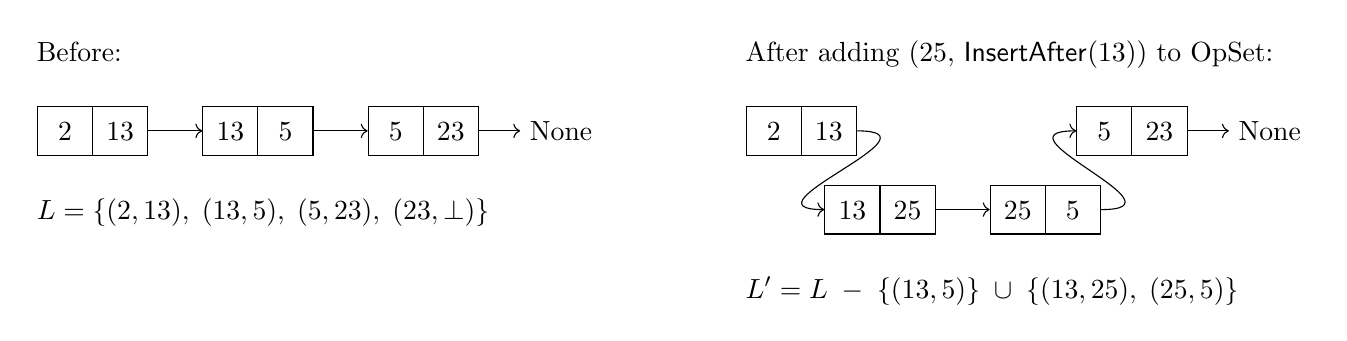
\begin{tikzpicture}
  \tikzstyle{every node}=[anchor=base,minimum width=7mm,text height=9pt,text depth=2pt]
  \node [anchor=west] at (-9,2) {Before:};
  \node [anchor=west] at (-9,0) {$L = \{ (2, 13),\; (13, 5),\; (5, 23),\; (23, \bot) \}$};
  \node [anchor=west] at (0,2) {After adding $(25,\, \mathsf{InsertAfter}(13))$ to OpSet:};
  \node [anchor=west] at (0,-1) {$L' = L \;-\; \{(13, 5)\} \;\cup\; \{(13, 25),\; (25, 5)\}$};
    \matrix [column sep={7mm,between origins},nodes=draw,matrix anchor=west] at (-9,1) {
    \node (l1a) {2};  & \node (l1b) {13}; &&
    \node (l2a) {13}; & \node (l2b) {5};  &&
    \node (l3a) {5};  & \node (l3b) {23}; &&
    \node (l4a) [draw=none] {None}; \\
  };
  \draw [->] (l1b) -- (l2a);
  \draw [->] (l2b) -- (l3a);
  \draw [->] (l3b) -- (l4a);
  \matrix [column sep={7mm,between origins},nodes=draw,matrix anchor=west] at (1,0) {
    \node (n1) {13}; & \node (n2) {25}; &&
    \node (n3) {25}; & \node (n4) {5}; \\
  };
  \matrix [column sep={7mm,between origins},nodes=draw,matrix anchor=west] at (0,1) {
    \node (r1a) {2};  & \node (r1b) {13}; &&&&&
    \node (r3a) {5};  & \node (r3b) {23}; &&
    \node (r4a) [draw=none] {None}; \\
  };
  \draw [->] (r1b.east) .. controls (2.7,1) and (0,0) .. (n1.west);
  \draw [->] (n2) -- (n3);
  \draw [->] (n4.east) .. controls (5.8,0) and (3.2,1) .. (r3a.west);
  \draw [->] (r3b) -- (r4a);
\end{tikzpicture}
\caption{Illustration of the interpretation of an $\mathsf{InsertAfter}$ operation.}\label{fig:list-insert}
\end{figure}

Note that $L$ never shrinks, it only ever grows through interpreting $\mathsf{InsertAfter}$ operations.
When a list element is removed by the function \textsc{removeListIndex} of Listing~\ref{fig:pseudocode}, the effect is that all values are removed from the list element in the element relation $E$, but the list element remains in $L$ as a \emph{tombstone}, so that any concurrent $\mathsf{InsertAfter}$ operations can still locate the referenced list position.

Thus, from a user's point of view a list element only exists if it has at least one associated value in the $E$ relation; any list elements without an associated value should be ignored.
On this basis we can now define the $\mathrm{idxKey}()$ function that is used in Listing~\ref{fig:pseudocode} to translate a list index into a list element ID:
\[ \mathrm{idxKey}_{E,\, L}(\mathit{obj}, \mathit{key}, i) \;=\; \left\{
   \arraycolsep=2pt \def\arraystretch{1.3}
   \begin{array}{llllll}
       \mathrm{idxKey}_{E,\, L}(\mathit{obj}, n, i-1) &
       \quad\text{if }\; i > 0 & \wedge & (\mathit{key}, n) \in L & \wedge &
       \exists\,\mathit{id}, \mathit{val}.\; (\mathit{id}, \mathit{obj}, \mathit{key}, \mathit{val}) \in E \\
       \mathrm{idxKey}_{E,\, L}(\mathit{obj}, n, i) &
       \quad\text{if }\; && (\mathit{key}, n) \in L & \wedge &
       \nexists\,\mathit{id}, \mathit{val}.\; (\mathit{id}, \mathit{obj}, \mathit{key}, \mathit{val}) \in E \\
       \mathit{key} &
       \quad\text{if }\; i = 0 & \wedge &&&
       \exists\,\mathit{id}, \mathit{val}.\; (\mathit{id}, \mathit{obj}, \mathit{key}, \mathit{val}) \in E \\
   \end{array} \right. \]
$\mathit{key}$ is initially the ID of the $\mathsf{MakeList}$ operation that created the list.
The function recursively moves along the linked list structure in $L$, decrementing the index for every list element that has an associated value, and not counting any list elements without associated value (which are treated as deleted).
Eventually, it returns the ID of the list element with the desired index.

\section{Discussion: Merging Text Edits}\label{sec:bad-merge}

The datatypes we have specified in \S~\ref{sec:datatypes} can support a wide range of applications.
For example, the list datatype can be used to implement a collaborative text editor: by treating the text as a list of individual characters, every edit can be expressed as a sequence of insertion or deletion operations on the list.

The problem of collaborative text editing has been studied extensively, using two main approaches: Operational Transformation and CRDTs.
We discuss this prior work in \S~\ref{sec:relwork}.
We will now highlight a scenario that, to our knowledge, has not been considered by any previous work on collaborative text editing.

Consider the execution illustrated in Figure~\ref{fig:bad-merge}.
In this example, two users are concurrently editing a text document that initially reads ``Hello!''.
The user on the left changes it to read ``Hello Alice!'', while concurrently the user on the right changes the document to read ``Hello Charlie!''.
When the concurrent edits are merged, the algorithm randomly interleaves the two insertions of ``~Alice'' and ``~Charlie'' character by character, resulting in an unreadable jumble of characters.

\begin{figure}
\centering
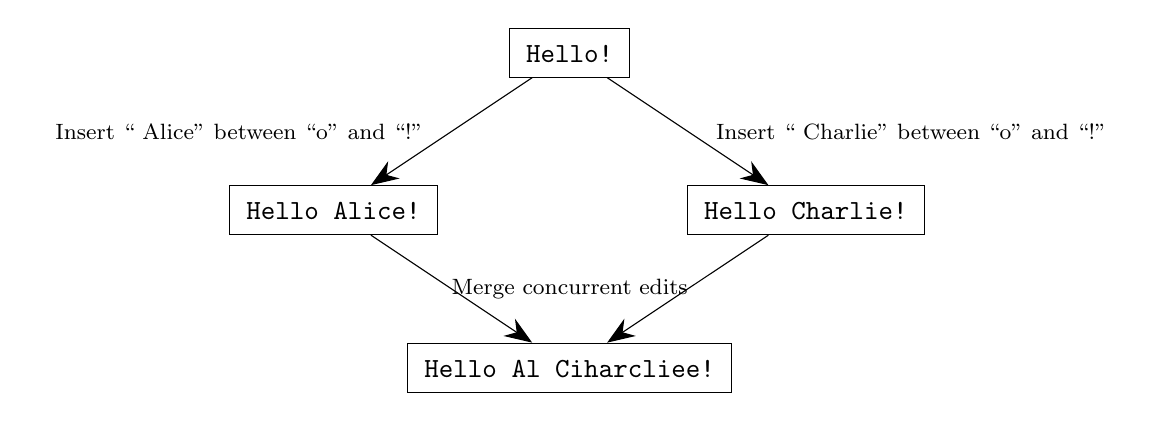
\begin{tikzpicture}
  \tikzstyle{box}=[rectangle,draw,inner xsep=6pt,text height=9pt,text depth=2pt]
  \tikzstyle{every path}=[draw,-{Stealth[length=3.5mm]}]
  \node [box] (start) at (3,4) {\texttt{Hello!}};
  \node [box] (left)  at (0,2) {\texttt{Hello Alice!}};
  \node [box] (right) at (6,2) {\texttt{Hello Charlie!}};
  \node [box] (merge) at (3,0) {\texttt{Hello Al Ciharcliee!}};
  \draw (start) to node [left,inner xsep=10pt,font=\footnotesize]  {Insert ``~Alice'' between ``o'' and ``!''} (left);
  \draw (start) to node [right,inner xsep=10pt,font=\footnotesize] {Insert ``~Charlie'' between ``o'' and ``!''} (right);
  \draw (left)  -- (merge);
  \draw (right) -- (merge);
  \node [text width=3cm,text badly centered,font=\footnotesize] at (3,1) {Merge concurrent edits};
\end{tikzpicture}
\caption{Two concurrent insertions at the same position are interleaved.}\label{fig:bad-merge}
\end{figure}

The problem is even worse if the concurrent insertions are not just a single word, but an entire paragraph or section.
In these cases, interleaving the users' insertions would most likely result in an entirely incomprehensible text that would have to be deleted and rewritten.
Even though the merge in Figure~\ref{fig:bad-merge} is so obviously undesirable, there is to our knowledge no formal specification of collaborative text editing that rules out such an interleaving of insertions.

\begin{theorem}\label{thm:attiya-allows-interleaving}
    The $\mathcal{A}_\textsf{strong}$ specification of collaborative text editing by Attiya et al. \cite{Attiya:2016kh} allows the outcome in Figure~\ref{fig:bad-merge}; that is, an algorithm that interleaves concurrent insertions at the same position may nevertheless satisfy the $\mathcal{A}_\textsf{strong}$ specification.
    Moreover, the text editing CRDT algorithms Logoot \cite{Weiss:2009ht,Weiss:2010hx} and LSEQ \cite{Nedelec:2016eo,Nedelec:2013ky} also allow this outcome.
\end{theorem}
\begin{proof}
    Follows directly from the respective definitions, which are all based on the idea of assigning each character a position in a totally ordered identifier space, such that the order of identifiers corresponds to the order of characters in the document.
    When a new character is inserted, it is assigned an identifier that lies somewhere between the identifiers of its predecessor and successor.
    However, when concurrent insertions with the same predecessor and successor are performed, those insertions are ordered arbitrarily.
    Repeated insertions within the same predecessor-successor interval may thus be interleaved arbitrarily.

    We also performed tests with open source implementations of Logoot \cite{AhmedNacer:2011ke,ReplicationBenchmark} and LSEQ \cite{LSEQTree,Nedelec:2016eo}, and observed this interleaving anomaly occurring in practice.
\end{proof}

Rather than interleaving characters, a better approach to merging is to keep all insertions by a particular user together as a continuous sequence.
With this constraint, there are two acceptable merged results in the example of Figure~\ref{fig:bad-merge}: either ``Hello Alice Charlie!'' or ``Hello Charlie Alice!''.
The choice between these two outcomes is arbitrary, as there is no \emph{a priori} requirement for one user's insertions to come before the other's.

\begin{theorem}\label{thm:no-interleaving}
    The list specification from \S~\ref{sec:datatypes} does not allow interleaving of concurrent insertions.
    That is, if one user inserts a character sequence $\langle x_1, x_2, \dots, x_n \rangle$ and another user concurrently inserts a character sequence $\langle y_1, y_2, \dots, y_m \rangle$ at the same position, the merged document contains either the character sequence $\langle x_1, x_2, \dots, x_n, y_1, y_2, \dots, y_m \rangle$ or the character sequence $\langle y_1, y_2, \dots, y_m, x_1, x_2, \dots, x_n \rangle$ at the specified position.
\end{theorem}
\begin{proof}
    We formalise the list specification and Theorem~\ref{thm:no-interleaving} using the Isabelle/HOL proof assistant~\cite{DBLP:conf/tphol/WenzelPN08}.
    \ifarxiv
        The formal proof development is summarised in Appendix~\ref{appendix:no-interleaving}.
    \else
        For space reasons, we elide the formal proof development; it is described in the extended version of this paper \cite{ExtendedVersion,AFP}.
    \fi
\end{proof}

For an informal argument why interleaving is ruled out, see Figure~\ref{fig:op-permutations}, which shows an editing scenario similar to Figure~\ref{fig:bad-merge}, but with the insertions of ``~Alice'' and ``~Charlie'' shortened to ``Al'' and ``Ch'' respectively.
The example contains four insertion operations (``A'', ``l'', ``C'', and ``h''), which can be ordered in six possible ways.
However, among the six possible operation orderings there are only two possible results: \texttt{ChAl} or \texttt{AlCh}.
Interleavings such as \texttt{CAhl} or \texttt{AChl} never occur.

In fact, the end result depends only on the relative ordering of the operations that insert ``A'' and ``C'', respectively.
All other operations can be reordered without affecting the outcome.
Thus, even if the inserted strings are longer than two characters, their relative ordering only depends on the IDs of their first character.
The remaining characters follow their initial character without interleaving.

Note that there are only six possible orderings of the four operations, and not $4! = 24$, because the Lamport timestamp ordering on identifiers (as given in \S~\ref{sec:system-model}) is a linear extension of the causal order.
In this example we assume that text is typed from left to right (that is, ``A'' is always inserted before ``l'', and ``C'' is inserted before ``h'').
This implies that the ID of the operation inserting ``l'' must be greater than that of the insertion of ``A'', and likewise the ``h'' insertion must be greater than the ``C'' insertion.

\begin{figure}
% ``A'', ``l'', ``C'', ``h''
% ``A'', ``C'', ``l'', ``h''
% ``A'', ``C'', ``h'', ``l''
% ``C'', ``A'', ``l'', ``h''
% ``C'', ``A'', ``h'', ``l''
% ``C'', ``h'', ``A'', ``l''
\setlength{\tabcolsep}{1pt}
\begin{tabular}{ll|ll|ll}
$\mathit{id}_1, \mathsf{InsertAfter}(\mathit{id}_0), \text{``A''}$ & $\rightarrow$ \texttt{A} &
$\mathit{id}_1, \mathsf{InsertAfter}(\mathit{id}_0), \text{``A''}$ & $\rightarrow$ \texttt{A} &
$\mathit{id}_1, \mathsf{InsertAfter}(\mathit{id}_0), \text{``A''}$ & $\rightarrow$ \texttt{A} \\
%%%%%%%%%%
$\mathit{id}_2, \mathsf{InsertAfter}(\mathit{id}_1), \text{``l''}$ & $\rightarrow$ \texttt{Al} &
$\mathit{id}_2, \mathsf{InsertAfter}(\mathit{id}_0), \text{``C''}$ & $\rightarrow$ \texttt{CA} &
$\mathit{id}_2, \mathsf{InsertAfter}(\mathit{id}_0), \text{``C''}$ & $\rightarrow$ \texttt{CA} \\
%%%%%%%%%%
$\mathit{id}_3, \mathsf{InsertAfter}(\mathit{id}_0), \text{``C''}$ & $\rightarrow$ \texttt{CAl} &
$\mathit{id}_3, \mathsf{InsertAfter}(\mathit{id}_1), \text{``l''}$ & $\rightarrow$ \texttt{CAl} &
$\mathit{id}_3, \mathsf{InsertAfter}(\mathit{id}_2), \text{``h''}$ & $\rightarrow$ \texttt{ChA} \\
%%%%%%%%%%
$\mathit{id}_4, \mathsf{InsertAfter}(\mathit{id}_3), \text{``h''}$ & $\rightarrow$ \texttt{ChAl} &
$\mathit{id}_4, \mathsf{InsertAfter}(\mathit{id}_2), \text{``h''}$ & $\rightarrow$ \texttt{ChAl} &
$\mathit{id}_4, \mathsf{InsertAfter}(\mathit{id}_1), \text{``l''}$ & $\rightarrow$ \texttt{ChAl} \\[6pt] \hline &&&&&\\[-6pt]
%%%%%%%%%%
$\mathit{id}_1, \mathsf{InsertAfter}(\mathit{id}_0), \text{``C''}$ & $\rightarrow$ \texttt{C} &
$\mathit{id}_1, \mathsf{InsertAfter}(\mathit{id}_0), \text{``C''}$ & $\rightarrow$ \texttt{C} &
$\mathit{id}_1, \mathsf{InsertAfter}(\mathit{id}_0), \text{``C''}$ & $\rightarrow$ \texttt{C} \\
%%%%%%%%%%
$\mathit{id}_2, \mathsf{InsertAfter}(\mathit{id}_0), \text{``A''}$ & $\rightarrow$ \texttt{AC} &
$\mathit{id}_2, \mathsf{InsertAfter}(\mathit{id}_0), \text{``A''}$ & $\rightarrow$ \texttt{AC} &
$\mathit{id}_2, \mathsf{InsertAfter}(\mathit{id}_1), \text{``h''}$ & $\rightarrow$ \texttt{Ch} \\
%%%%%%%%%%
$\mathit{id}_3, \mathsf{InsertAfter}(\mathit{id}_2), \text{``l''}$ & $\rightarrow$ \texttt{AlC} &
$\mathit{id}_3, \mathsf{InsertAfter}(\mathit{id}_1), \text{``h''}$ & $\rightarrow$ \texttt{ACh} &
$\mathit{id}_3, \mathsf{InsertAfter}(\mathit{id}_0), \text{``A''}$ & $\rightarrow$ \texttt{ACh} \\
%%%%%%%%%%
$\mathit{id}_4, \mathsf{InsertAfter}(\mathit{id}_1), \text{``h''}$ & $\rightarrow$ \texttt{AlCh} &
$\mathit{id}_4, \mathsf{InsertAfter}(\mathit{id}_2), \text{``l''}$ & $\rightarrow$ \texttt{AlCh} &
$\mathit{id}_4, \mathsf{InsertAfter}(\mathit{id}_3), \text{``l''}$ & $\rightarrow$ \texttt{AlCh} \\
\end{tabular}
\caption{All possible operation orderings when the strings ``Al'' (for ``Alice'') and ``Ch'' (for ``Charlie'') are concurrently inserted at the same position.
The operation IDs are arbitrary; we only require that $id_0 < id_1 < id_2 < id_3 < id_4$.}\label{fig:op-permutations}
\end{figure}

\begin{theorem}
    The OpSet list specification from \S~\ref{sec:datatypes} is strictly stronger than the $\mathcal{A}_\textsf{strong}$ specification of Attiya et al \cite{Attiya:2016kh}.
    That is, any algorithm that satisfies the list specification given in \S~\ref{sec:datatypes} also satisfies $\mathcal{A}_\textsf{strong}$, but the converse is not true.
\end{theorem}
\begin{proof}
    We formalise the $\mathcal{A}_\textsf{strong}$ specification with Isabelle/HOL, and produce a mechanically verified proof that every possible execution of the list specification from \S~\ref{sec:datatypes} satisfies all conditions of $\mathcal{A}_\textsf{strong}$.
    \ifarxiv
        The formal proof development is summarised in Appendix~\ref{appendix:attiya-spec}.
    \else
        The formal proof development is described in the extended version of this paper \cite{ExtendedVersion,AFP}.
    \fi
    The fact that our specification is \emph{strictly} stronger follows from Theorems~\ref{thm:attiya-allows-interleaving} and~\ref{thm:no-interleaving}.
\end{proof}

\begin{theorem}
    The RGA algorithm \cite{Roh:2011dw} satisfies the OpSet list specification introduced in this paper, while Logoot \cite{Weiss:2009ht,Weiss:2010hx} and LSEQ \cite{Nedelec:2016eo,Nedelec:2013ky} do not.
\end{theorem}
\begin{proof}
    We use Isabelle/HOL to prove that RGA satisfies our specification, as described in
    \ifarxiv
        Appendix~\ref{appendix:rga}.
    \else
        the extended version of this paper \cite{ExtendedVersion,AFP}.
    \fi
    Our Isabelle/HOL implementation of RGA is based on the formalisation that we developed in previous work \cite{Gomes:2017vo,Gomes:2017gy}.
    The fact that Logoot and LSEQ do not satisfy our specification follows directly from Theorems~\ref{thm:attiya-allows-interleaving} and~\ref{thm:no-interleaving}.
\end{proof}

\section{Specifying a Tree Datatype}\label{sec:tree}

Tree data structures are useful in many applications: for example, file systems (consisting of directories and files) and XML or JSON documents are trees.
In this section we build upon the data structures of \S~\ref{sec:datatypes} to specify a collaboratively editable tree datatype.
Branch nodes in this tree may be either maps or lists, and leaf nodes are primitive values (wrapped in a $\mathsf{MakeVal}$ operation).

Unlike previous CRDTs for tree data structures \cite{Martin:2010ih,Kleppmann:2016ve}, our datatype supports an \emph{atomic move} operation, which can move an entire subtree to a new location, or rename a key in a map, or reorder items in a list.
Moving an item is not the same as deleting it and re-inserting it in a new location: if two users concurrently delete and re-insert the same item, it would be duplicated.
On the other hand, if two users concurrently move the same item to different locations, the move operation with the greater ID will determine the item's final location.

A tree is a restricted form of the object graph specified in \S~\ref{sec:datatypes}.
First, we require that there is a designated root object: assume that we have an operation ID $\mathsf{root}$ that is less than all other operation IDs (according to the total order on identifiers, introduced in \S~\ref{sec:system-model}).
Further assume that for any OpSet $O$ specifying a tree, we have either $(\mathsf{root},\, \mathsf{MakeList}) \in O$ or $(\mathsf{root},\, \mathsf{MakeMap}) \in O$, depending on whether the root node is a list or a map.
We define an object $x$ to be the \emph{parent} of an object $y$ if one of the values in $x$ is a reference to $y$.
The \emph{ancestor} relation is the transitive closure of the parent relation, defined using the element relation $E$:
\begin{align*}
    \mathrm{parent}(E,\, i) &=
    \begin{cases}
        \big\{ (\mathit{obj}, \mathit{val}) \mid \exists\,\mathit{id}, \mathit{key}.\;
            (\mathit{id}, \mathit{obj}, \mathit{key}, \mathit{val}) \in E \big\} & \text{if } i=1 \\
        \big\{ (x, z) \mid (x, y) \in \mathrm{parent}(E,\, i-1) \;\wedge\;
            (y, z) \in \mathrm{parent}(E,\, 1) \big\} & \text{if } i > 1
    \end{cases} \\[8pt]
    \mathrm{ancestor}(E) &= \bigcup_{i \;\geq\; 1} \mathrm{parent}(E,\, i)
\end{align*}

An object graph is a tree if the root has no parent, every non-root node has exactly one parent, and if the ancestor relation has no cycles.
We can redefine the operation interpretations from \S~\ref{sec:datatypes-interp} to preserve this tree invariant.
In fact, it is sufficient to redefine the interpretation of $\mathsf{Assign}$, and leave the interpretation of the other five operation types unchanged:
\begin{align*}
    \mathrm{interp}&\big[(E,\, L),\; (\mathit{id},\, \mathsf{Assign}(\mathit{obj}, \mathit{key}, \mathit{val}, \mathit{prev})) \big] \;=\\
    & \left\{
    \arraycolsep=0pt \def\arraystretch{1.5}
    \begin{array}{l}
        (E,\, L) \qquad \text{if } (\mathit{val},\, \mathit{obj}) \in \mathrm{ancestor}(E) \\[2pt]
        \Big( \big\{ (\mathit{id}', \mathit{obj}', \mathit{key}', \mathit{val}') \in E \mid
        \mathit{id}' \notin \mathit{prev} \wedge \mathit{val}' \neq \mathit{val} \big\} \;\cup\;
        \big\{ (\mathit{id}, \mathit{obj}, \mathit{key}, \mathit{val}) \big\},\; L \Big) \\
        \hphantom{(E,\, L)} \qquad \text{if } (\mathit{val},\, \mathit{obj}) \notin \mathrm{ancestor}(E)
    \end{array} \right.
\end{align*}

This definition differs in two ways from that in \S~\ref{sec:datatypes-interp}.
Firstly, the operation has no effect if the value $\mathit{val}$ is already an ancestor of the proposed parent $\mathit{obj}$, since the operation would otherwise introduce a cycle.
Secondly, any existing tuple in $E$ that references the same value $\mathit{val}$ is removed, preserving the invariant that every non-root node must have exactly one parent.

Intuitively, this interpretation of $\mathsf{Assign}$ performs an atomic move whenever $\mathit{val}$ is the ID of an existing object in the tree; in that case, it is moved from its existing position to the key $\mathit{key}$ in the object $\mathit{obj}$.
If $\mathit{val}$ does not currently exist in the tree (e.g.\ because it has just been created), the operation behaves like conventional assignment.

\subsection{Discussion: Subtree Move Conflicts}

In a replicated tree datatype with move operations, concurrent moves may conflict in various ways \cite{Najafzadeh:2017vk,AhmedNacer:2012us,Tao:2015gd}.
For example, two different operations may concurrently move the same object to different positions; we resolve this conflict by letting the operation with the greatest identifier ``win''.
Intuitively, we can think of the location of an object in the tree as being determined by a last-writer-wins register, and a move operation overwrites that register.

\begin{figure}
\centering
\begin{tikzpicture}
  \tikzstyle{arrow}=[draw,-{Stealth[length=3.5mm]}]
  \node [rectangle,draw] (start) at (4,4) {
      \begin{tikzpicture}
      \node {$\mathsf{root}$} [level distance=9mm] child {node {$a$}} child {node {$b$}};
      \end{tikzpicture}
  };
  \node [rectangle,draw] (left) at (1,2) {
      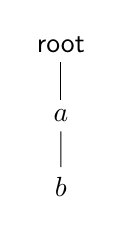
\begin{tikzpicture}
      \node {$\mathsf{root}$} [level distance=9mm] child {node {$a$} child {node {$b$}}};
      \end{tikzpicture}
  };
  \node [rectangle,draw] (right) at (7,2) {
      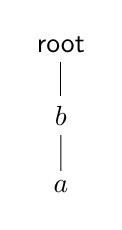
\begin{tikzpicture}
      \node {$\mathsf{root}$} [level distance=9mm] child {node {$b$} child {node {$a$}}};
      \end{tikzpicture}
  };
  \node [rectangle,draw] (merge) at (4,0) { ? };
  \node at (0,4) {$(\mathit{id}_1,\, \mathsf{Assign}(a,\, \mathit{key}_1,\, b,\, \emptyset))$};
  \node at (8,4) {$(\mathit{id}_2,\, \mathsf{Assign}(b,\, \mathit{key}_2,\, a,\, \emptyset))$};
  \draw [arrow] (start.west) -- (left);
  \draw [arrow] (start.east) -- (right);
  \draw [arrow] (left)  -- (merge.north west);
  \draw [arrow] (right) -- (merge.north east);
  \node at (4,1) {merge};
\end{tikzpicture}
\caption{Initially, $a$ and $b$ are siblings. On one node, $b$ is moved to be a child of $a$, while concurrently on another node,
$a$ is moved to be a child of $b$. What should the final outcome be?}\label{fig:concurrent-move}
\end{figure}

A more subtle kind of conflict is illustrated in Figure~\ref{fig:concurrent-move}.
Here, two different objects $a$ and $b$, which are originally siblings, are concurrently moved to be children of each other.
If the move semantics are not defined carefully, it could happen that $a$ and $b$ form a cycle, violating the tree invariant.
Our interpretation function for $\mathsf{Assign}$ handles this situation based on the ordering of the operation IDs $\mathit{id}_1$ and $\mathit{id}_2$.
Since operations are interpreted in order of ascending identifier, one of the two (say, $\mathit{id}_1$) is interpreted first.
When the second ($\mathit{id}_2$) is subsequently interpreted, $a$ is already an ancestor of $b$, and thus the second operation has no effect.

On some nodes, operation $\mathit{id}_2$ may be applied first, and $\mathit{id}_1$ applied later.
In this case, the user will first observe $b$ becoming a child of $a$, and later observe their positions being swapped (with the effect of $\mathit{id}_2$ being undone).

\section{Related Work}\label{sec:relwork}

Algorithms for collaboratively editing a shared data structure have been the topic of active research for approximately 30 years, under the headings of Operational Transformation \cite{Ellis:1989ue,Nichols:1995fd,Ressel:1996wx,Sun:1998un,Sun:1998vf,Suleiman:1997gl,Suleiman:1998eu,Vidot:2000ch,Imine:2003ks,Li:2004er,Li:2008hw,Oster:2006tr} and CRDTs \cite{Shapiro:2011wy,Shapiro:2011un,Roh:2011dw,Preguica:2009fz,Oster:2006wj,Weiss:2010hx,Nedelec:2013ky,Nedelec:2016eo,Grishchenko:2014eh,Kleppmann:2016ve}.

However, throughout this time, the exact consistency properties provided by the algorithms have been somewhat unclear.
For example, Sun et al.~\cite{Sun:1998un} identified three desirable properties that they articulated informally: \emph{convergence}, \emph{causality preservation}, and \emph{intention preservation}.
While the definition of the first two properties is fairly unambiguous, the definition of ``intention preservation'' leaves much more room for interpretation.
Sun et al.\ define it as follows \cite{Sun:1998un}:
\begin{displayquote}
For any operation $O$, the effects of executing $O$ at all sites are the same as the intention of $O$, and the effect of executing $O$ does not change the effects of independent operations.
\end{displayquote}
where the term \emph{intention} is in turn defined as:
\begin{displayquote}
The intention of an operation $O$ is the execution effect which can be achieved by applying $O$ on the document state from which $O$ was generated.
\end{displayquote}
Efforts to formally specify and verify the semantics of replicated datatypes have replaced informal statements of this type with more precise definitions of consistency properties.

\subsection{Specification and Verification}

Bieniusa et al.~\cite{Bieniusa:2012gt} articulate a \emph{principle of permutation equivalence} that partially specifies the expected semantics of replicated datatypes, but which leaves some combinations of operations unspecified.
Burckhardt et al.~\cite{Burckhardt:2014ft} give a complete specification of CRDT counters, registers, and sets, and show how to verify that algorithms satisfy these specifications in hand-written proofs.
Zeller et al.~\cite{Zeller:2014fl} formalise the same datatypes using Isabelle/HOL and provide mechanised proofs of their correctness.
These papers do not consider lists, maps, or tree datatypes.

Gomes et al.~\cite{Gomes:2017gy} establish a formal verification framework for CRDTs in Isabelle/HOL, and verify the strong eventual consistency properties (in particular, convergence) of a list, set, and counter datatype.
However, the work does not specify the datatype semantics beyond the convergence property.

Attiya et al.~\cite{Attiya:2016kh} give two specifications of collaborative text editing ($\mathcal{A}_\textsf{strong}$ and $\mathcal{A}_\textsf{weak}$), prove that the RGA CRDT \cite{Roh:2011dw} satisfies $\mathcal{A}_\textsf{strong}$, and conjecture that the Operational Transformation algorithm Jupiter \cite{Nichols:1995fd} satisfies $\mathcal{A}_\textsf{weak}$.
Wei et al.~\cite{Wei:2017tg} complete the proof that Jupiter satisfies $\mathcal{A}_\textsf{weak}$.

XXX: also~\cite{DBLP:conf/popl/BurckhardtGYZ14, DBLP:conf/atva/MukundRS15, DBLP:conf/coordination/GadducciMR17, DBLP:conf/popl/GotsmanYFNS16}

\subsection{Collaborative Tree Datatypes}

For collaborative editing of tree data structures, several CRDTs \cite{Martin:2010ih,Kleppmann:2016ve} and Operational Transformation algorithms \cite{Jungnickel:2016cb,Ignat:2003jy,Davis:2002iv} have been proposed.
However, most of them only consider insertion and deletion of tree nodes, but do not support a move operation.

As explained in Section~\ref{sec:tree}, supporting an operation that can move a subtree to a new location within a tree raises the possibility of some particular conflicts that need to be handled.
Ahmed-Nacer et al.~\cite{AhmedNacer:2012us} survey approaches to handling these conflicts without providing concrete algorithms.
Tao et al.~\cite{Tao:2015gd} propose handling conflicting move operations by allowing the same object to appear in more than one location; thus, their datatype is strictly a DAG, not a tree.

Najafzadeh~\cite{Najafzadeh:2017vk} asserts that concurrent move operations on a tree cannot safely be implemented in a CRDT, since the precondition of a move operation is not stable.
The proposed solution in this work is to use locks to globally synchronise move operations, thus preventing a scenario such as that in Figure~\ref{fig:concurrent-move} from ever occurring.
However, the resulting datatype is not strictly a CRDT, since some operations require strongly consistent synchronisation.

To our knowledge, our move semantics specified in Section~\ref{sec:tree} is the first definition of such an operation on a fully asynchronous tree CRDT.
We avoid the apparent contradiction with Najafzadeh's assertion by evaluating the precondition $(\mathit{val},\, \mathit{obj}) \notin \mathrm{ancestor}(E)$ at the same time as applying the operation, rather than at the time when the operation is generated, and by applying all operations in the OpSet in a deterministic order.

\subsection{Ordered Sets of Operations}

Baquero et al.~\cite{Baquero:2014ed} and Grishchenko~\cite{Grishchenko:2014eh} have previously proposed representing CRDTs in terms of a partially-ordered log of operations (where the partial order captures the causal relationships between operations).
Our OpSet is a straightforward variant of this idea, in which we define the total order on identifiers to be a linear extension of the partial order that captures causality.
This linear extension is well-known and goes back to Lamport~\cite{Lamport:1978jq}.

Our approach of sequentially interpreting operations, in order of $\mathit{id}$, is reminiscent of the concept of \emph{serializability} in databases: the data structure obtained by interpreting an OpSet is equal to the outcome of applying the operations in their serial order, even if the execution that produced the OpSet was in fact concurrent.
However, conventional transaction serializability requires synchronous coordination between replicas \cite{Davidson:1985hv}.
We circumvent this limitation, and hence allow nodes to make progress while offline, by allowing the interpretation of an operation to change if another operation with a lower ID is delivered.


\section{Conclusion}

In this work we have introduced Operation Sets (OpSets), a simple but expressive approach for specifying the semantics of replicated datatypes.
We specified a variety of common, composable replicated datatypes in the OpSets model, and used Isabelle/HOL to formally reason about their properties.
We have also shown how the OpSet abstraction can be used to reason about existing replication algorithms, and developed a new specification to highlight an interleaving anomaly that affects some existing collaborative text editing algorithms.
Finally we demonstrated how the OpSet model to can be used to develop new specifications to support algorithm design, and developed a specification for an atomic move operation in a tree CRDT.

The OpSets approach is a form of executable specification that precisely defines the permitted states of a replica after some set of updates have been applied.
The simplicity of our approach builds on sequential OpSet interpretation: operations are applied in strict ascending order of ID.
This property is very useful as it trivially ensures convergence, and it simplifies reasoning about specifications and invariants for CRDTs.
In contrast, the traditional approach requires operations to be defined in a way that is commutative, increasing their complexity.
We took advantage of the ease of specification to demonstrate the correspondence between sequential specification and commutative implementation, proving that the RGA CRDT satisfies our OpSet specification of lists.
For future work it will be interesting to further explore this correspondence for other datatypes; in particular, we hypothesise that it is possible to derive a tree CRDT with a commutative move operation from the specification in \S~\ref{sec:tree}.

%More generally, one can regard the OpSet as a \emph{database of facts}, containing all changes ever made to the shared data, and the interpretation function a \emph{query} over this database, with the resulting datatype being a \emph{materialized view} in database terminology.
%When new operations are added to an OpSet $O$, computing the corresponding change to $\llbracket O \rrbracket$ is a \emph{materialized view maintenance} problem, which has been studied extensively in the database literature \cite{Gupta:1999uz}.
%We have found that thinking about replicated datatypes as materialized views onto an OpSet a useful perspective for understanding and improving replication algorithms, and in future work we aim to explore this idea more fully.

\subsection*{Acknowledgements}

The authors wish to acknowledge the support of The Boeing Company,
the EPSRC ``REMS: Rigorous Engineering for Mainstream Systems'' programme grant (EP/K008528), and
the EPSRC ``Interdisciplinary Centre for Finding, Understanding and Countering Crime in the Cloud'' grant (EP/M020320).
We thank Nathan Chong, Peter Sewell, and KC Sivaramakrishnan for their helpful feedback on this paper.

\newpage

\bibliographystyle{plainnat}
\bibliography{references}{}

\newpage

\appendix

\section{Introduction to Isabelle/HOL}
\label{sect:appendix:isabelle}

In the following appendices we provide a copy of the Isabelle/HOL definitions and proof statements that support the central claims in the paper.
To help any readers who are not familiar with Isabelle/HOL, we first provide a brief introduction to the key concepts and syntax, taken from our previous work \cite{Gomes:2017gy}.
A more detailed introduction can be found in the standard tutorial material~\cite{DBLP:books/sp/NipkowK14}.

\paragraph{Syntax of expressions.}

Isabelle/HOL is a logic with a strict, polymorphic, inferred type system.
\emph{Function types} are written $\tau_1 \Rightarrow \tau_2$, and are inhabited by \emph{total} functions, mapping elements of $\tau_1$ to elements of $\tau_2$.
We write $\tau_1 \times \tau_2$ for the \emph{product type} of $\tau_1$ and $\tau_2$, inhabited by pairs of elements of type $\tau_1$ and $\tau_2$, respectively.
\emph{Type operators} are applied to arguments in reverse order: $\tau\ \isa{list}$ denotes the type of lists of elements of type $\tau$, and $\tau\ \isa{set}$ denotes the type of mathematical (i.e., potentially infinite) sets of type $\tau$, for instance.
Type variables are written in lowercase, and preceded with a prime: ${\isacharprime}a \Rightarrow {\isacharprime}a$ denotes the type of a polymorphic identity function, for example.
\emph{Tagged union} types are introduced with the $\isacommand{datatype}$ keyword, with \emph{constructors} of these types usually written with an initial upper case letter.

In Isabelle/HOL's term language we write $\isa{t} \mathbin{::} \tau$ for a \emph{type ascription}, constraining the type of the term $\isa{t}$ to the type $\tau$.
We write $\lambda{x}.\: t$ for an anonymous function mapping an argument $\isa{x}$ to $\isa{t(x)}$, and write the application of term $\isa{t}$ with function type to an argument $\isa{u}$ as $\isa{t\ u}$.
Terms of list type are introduced using one of two constructors: the empty list $[\,]$ or `nil', and the infix operator $\isa{\#}$ which is pronounced ``cons'', and which prepends an element to an existing list.
We use $[t_1, \ldots, t_n]$ as syntactic sugar for a list literal, and $\isa{xs} \mathbin{\isacharat} \isa{ys}$ to express the concatenation (appending) of two lists $\isa{xs}$ and $\isa{ys}$.
We write $\{\,\}$ for the empty set, and use usual mathematical notation for set union, disjunction, membership tests, and so on: $\isa{t} \cup \isa{u}$, $\isa{t} \cap \isa{u}$, and $\isa{x} \in \isa{t}$.
We write $t \longrightarrow s$ for logical implication between formulae (terms of type $\isa{bool}$).
Strictly speaking Isabelle is a logical framework, providing a weak meta-logic within which object logics are embedded, including the Isabelle/HOL object logic that we use in this work.
Accordingly, the implication arrow of Isabelle's meta-logic, $\isa{t} \Longrightarrow \isa{u}$, is required in certain contexts over the object-logic implication arrow, $t \longrightarrow s$, already introduced.
However, for purposes of an intuitive understanding, the two forms of implication can be regarded as equivalent by the reader, with the requirement to use one over the other merely being an implementation detail of Isabelle itself.
We will sometimes use the shorthand ${\isasymlbrakk}\isa{H}_1{\isacharsemicolon}\ \ldots{\isacharsemicolon}\ \isa{H}_n{\isasymrbrakk}\ {\isasymLongrightarrow}\ C$ instead of iterated meta-logic implications, i.e., $H_1\ {\isasymLongrightarrow}\ \ldots\ {\isasymLongrightarrow}\ H_n\ {\isasymLongrightarrow}\ C$.

\paragraph{Definitions and theorems.}

New non-recursive definitions are entered into Isabelle's global context using the $\mathbf{definition}$ keyword.
Recursive functions are defined using the $\mathbf{fun}$ keyword, and support \emph{pattern matching} on their arguments.
All functions are total, and therefore every recursive function must be provably terminating.
All termination proofs in this work are generated automatically by Isabelle itself.

\emph{Inductive relations} are defined with the $\mathbf{inductive}$ keyword.
For example, the definition
\begin{isabelle}
\isacommand{inductive} only-fives\ {\isacharcolon}{\isacharcolon}\ {\isachardoublequoteopen}nat\ list\ {\isasymRightarrow}\ bool{\isachardoublequoteclose}\ \isakeyword{where} \\
~~~~{\isachardoublequoteopen}only-fives\ {\isacharbrackleft}{\isacharbrackright}{\isachardoublequoteclose}\ {\isacharbar}\\
~~~~{\isachardoublequoteopen}{\isasymlbrakk}\ only-fives\ xs\ {\isasymrbrakk}\ {\isasymLongrightarrow}\ only-fives {\isacharparenleft}5\#xs{\isacharparenright}{\isachardoublequoteclose}
\end{isabelle}
\noindent %dpm: spacing above
introduces a new constant $\isa{only-fives}$ of type $\isa{nat list} \Rightarrow \isa{bool}$.
The two clauses in the body of the definition enumerate the conditions under which $\isa{only-fives}\ \isa{xs}$ is true, for arbitrary $\isa{xs}$: firstly, $\isa{only-fives}$ is true for the empty list; and secondly, if you know that $\isa{only-fives}\ \isa{xs}$ is true for some $\isa{xs}$, then you can deduce that $\isa{only-fives}\ (5\#\isa{xs})$ (i.e., $\isa{xs}$ prefixed with the number 5) is also true.
Moreover, $\isa{only-fives}\ \isa{xs}$ is true in no other circumstances---it is the \emph{smallest} relation closed under the rules defining it.
In short, the clauses above state that $\isa{only-fives}\ \isa{xs}$ holds exactly in the case where $\isa{xs}$ is a (potentially empty) list containing only repeated copies of the natural number $5$.

Lemmas, theorems, and corollaries can be asserted using the $\isacommand{lemma}$, $\isacommand{theorem}$, and $\isacommand{corollary}$ keywords, respectively.
There is no semantic difference between these keywords in Isabelle.
For example,
\begin{isabelle}
\isacommand{theorem} only-fives-concat{\isacharcolon} \\
~~~~\isakeyword{assumes}\ only-fives\ xs \isakeyword{and}\ only-fives\ ys\\
~~~~\isakeyword{shows}\ only-fives\ (xs \isacharat ys)
\end{isabelle}
\noindent %dpm: spacing above
conjectures that if $\isa{xs}$ and $\isa{ys}$ are both lists of fives, then their concatenation $xs \mathbin{\isacharat} ys$ is also a list of fives.
Isabelle then requires that this claim be proved by using one of its proof methods, for example by induction.
Some proofs can be automated, whilst others require the user to provide explicit reasoning steps.
The theorem is assigned a name, here $\isa{only-fives-concat}$, so that it may be referenced in later proofs.

\newpage

\isafoldtag{proof}
%
\begin{isabellebody}%
\setisabellecontext{OpSet}%
%
\isamarkupsection{Abstract OpSet%
}
\isamarkuptrue%
%
\begin{isamarkuptext}%
In this section, we define a general-purpose OpSet abstraction that is not
specific to any one particular datatype. We develop a library of useful lemmas
that we can build upon later when reasoning about a specific datatype.%
\end{isamarkuptext}\isamarkuptrue%
%
\isadelimtheory
%
\endisadelimtheory
%
\isatagtheory
\isacommand{theory}\isamarkupfalse%
\ OpSet\isanewline
\ \ \isakeyword{imports}\ Main\isanewline
\isakeyword{begin}%
\endisatagtheory
{\isafoldtheory}%
%
\isadelimtheory
%
\endisadelimtheory
%
\isamarkupsubsection{OpSet definition%
}
\isamarkuptrue%
%
\begin{isamarkuptext}%
An OpSet is a set of (ID, operation) pairs with an associated total order
on IDs (represented here with the ``linorder'' typeclass), and satisfying the
following properties:
\begin{enumerate}
\item The ID is unique (that is, if any two pairs in the set have the same ID,
then their operation is also the same).
\item If the operation references the IDs of any other operations, those
referenced IDs are less than that of the operation itself, according to the
total order on IDs. To avoid assuming anything about the structure of operations
here, we use a function ``deps'' that returns the set of dependent IDs for a given
operation. This requirement is a weak expression of causality: an operation can
only depend on causally prior operations, and by making the total order on IDs
a linear extension of the causal order, this requirement is easily satisfied.
\item The OpSet is finite (but we do not assume any particular maximum size).
\end{enumerate}%
\end{isamarkuptext}\isamarkuptrue%
\isacommand{locale}\isamarkupfalse%
\ opset\ {\isacharequal}\isanewline
\ \ \isakeyword{fixes}\ opset\ {\isacharcolon}{\isacharcolon}\ {\isachardoublequoteopen}{\isacharparenleft}{\isacharprime}oid{\isacharcolon}{\isacharcolon}{\isacharbraceleft}linorder{\isacharbraceright}\ {\isasymtimes}\ {\isacharprime}oper{\isacharparenright}\ set{\isachardoublequoteclose}\isanewline
\ \ \ \ \isakeyword{and}\ deps\ \ {\isacharcolon}{\isacharcolon}\ {\isachardoublequoteopen}{\isacharprime}oper\ {\isasymRightarrow}\ {\isacharprime}oid\ set{\isachardoublequoteclose}\isanewline
\ \ \isakeyword{assumes}\ unique{\isacharunderscore}oid{\isacharcolon}\ {\isachardoublequoteopen}{\isacharparenleft}oid{\isacharcomma}\ op{\isadigit{1}}{\isacharparenright}\ {\isasymin}\ opset\ {\isasymLongrightarrow}\ {\isacharparenleft}oid{\isacharcomma}\ op{\isadigit{2}}{\isacharparenright}\ {\isasymin}\ opset\ {\isasymLongrightarrow}\ op{\isadigit{1}}\ {\isacharequal}\ op{\isadigit{2}}{\isachardoublequoteclose}\isanewline
\ \ \ \ \isakeyword{and}\ ref{\isacharunderscore}older{\isacharcolon}\ {\isachardoublequoteopen}{\isacharparenleft}oid{\isacharcomma}\ oper{\isacharparenright}\ {\isasymin}\ opset\ {\isasymLongrightarrow}\ ref\ {\isasymin}\ deps\ oper\ {\isasymLongrightarrow}\ ref\ {\isacharless}\ oid{\isachardoublequoteclose}\isanewline
\ \ \ \ \isakeyword{and}\ finite{\isacharunderscore}opset{\isacharcolon}\ {\isachardoublequoteopen}finite\ opset{\isachardoublequoteclose}%
\begin{isamarkuptext}%
We prove some lemmas about OpSets. In particular, any subset of an OpSet
is also a valid OpSet. This is the case because although an operation can
depend on causally prior operations, the OpSet does not require those prior
operations to actually exist. This weak assumption makes the OpSet model
more general and simplifies reasoning about OpSets.%
\end{isamarkuptext}\isamarkuptrue%
\isacommand{lemma}\isamarkupfalse%
\ opset{\isacharunderscore}subset{\isacharcolon}\isanewline
\ \ \isakeyword{assumes}\ {\isachardoublequoteopen}opset\ Y\ deps{\isachardoublequoteclose}\isanewline
\ \ \ \ \isakeyword{and}\ {\isachardoublequoteopen}X\ {\isasymsubseteq}\ Y{\isachardoublequoteclose}\isanewline
\ \ \isakeyword{shows}\ {\isachardoublequoteopen}opset\ X\ deps{\isachardoublequoteclose}\isanewline
%
\isadelimproof
%
\endisadelimproof
%
\isatagproof
\isacommand{proof}\isamarkupfalse%
\isanewline
\ \ \isacommand{fix}\isamarkupfalse%
\ oid\ op{\isadigit{1}}\ op{\isadigit{2}}\isanewline
\ \ \isacommand{assume}\isamarkupfalse%
\ {\isachardoublequoteopen}{\isacharparenleft}oid{\isacharcomma}\ op{\isadigit{1}}{\isacharparenright}\ {\isasymin}\ X{\isachardoublequoteclose}\ \isakeyword{and}\ {\isachardoublequoteopen}{\isacharparenleft}oid{\isacharcomma}\ op{\isadigit{2}}{\isacharparenright}\ {\isasymin}\ X{\isachardoublequoteclose}\isanewline
\ \ \isacommand{thus}\isamarkupfalse%
\ {\isachardoublequoteopen}op{\isadigit{1}}\ {\isacharequal}\ op{\isadigit{2}}{\isachardoublequoteclose}\isanewline
\ \ \ \ \isacommand{using}\isamarkupfalse%
\ assms\ \isacommand{by}\isamarkupfalse%
\ {\isacharparenleft}meson\ opset{\isachardot}unique{\isacharunderscore}oid\ set{\isacharunderscore}mp{\isacharparenright}\isanewline
\isacommand{next}\isamarkupfalse%
\isanewline
\ \ \isacommand{fix}\isamarkupfalse%
\ oid\ oper\ ref\isanewline
\ \ \isacommand{assume}\isamarkupfalse%
\ {\isachardoublequoteopen}{\isacharparenleft}oid{\isacharcomma}\ oper{\isacharparenright}\ {\isasymin}\ X{\isachardoublequoteclose}\ \isakeyword{and}\ {\isachardoublequoteopen}ref\ {\isasymin}\ deps\ oper{\isachardoublequoteclose}\isanewline
\ \ \isacommand{thus}\isamarkupfalse%
\ {\isachardoublequoteopen}ref\ {\isacharless}\ oid{\isachardoublequoteclose}\isanewline
\ \ \ \ \isacommand{using}\isamarkupfalse%
\ assms\ \isacommand{by}\isamarkupfalse%
\ {\isacharparenleft}meson\ opset{\isachardot}ref{\isacharunderscore}older\ set{\isacharunderscore}rev{\isacharunderscore}mp{\isacharparenright}\isanewline
\isacommand{next}\isamarkupfalse%
\isanewline
\ \ \isacommand{show}\isamarkupfalse%
\ {\isachardoublequoteopen}finite\ X{\isachardoublequoteclose}\isanewline
\ \ \ \ \isacommand{using}\isamarkupfalse%
\ assms\ opset{\isachardot}finite{\isacharunderscore}opset\ finite{\isacharunderscore}subset\ \isacommand{by}\isamarkupfalse%
\ blast\isanewline
\isacommand{qed}\isamarkupfalse%
%
\endisatagproof
{\isafoldproof}%
%
\isadelimproof
\isanewline
%
\endisadelimproof
\isanewline
\isacommand{lemma}\isamarkupfalse%
\ opset{\isacharunderscore}insert{\isacharcolon}\isanewline
\ \ \isakeyword{assumes}\ {\isachardoublequoteopen}opset\ {\isacharparenleft}insert\ x\ ops{\isacharparenright}\ deps{\isachardoublequoteclose}\isanewline
\ \ \isakeyword{shows}\ {\isachardoublequoteopen}opset\ ops\ deps{\isachardoublequoteclose}\isanewline
%
\isadelimproof
%
\endisadelimproof
%
\isatagproof
\isacommand{using}\isamarkupfalse%
\ assms\ opset{\isacharunderscore}subset\ \isacommand{by}\isamarkupfalse%
\ blast%
\endisatagproof
{\isafoldproof}%
%
\isadelimproof
\isanewline
%
\endisadelimproof
\isanewline
\isacommand{lemma}\isamarkupfalse%
\ opset{\isacharunderscore}sublist{\isacharcolon}\isanewline
\ \ \isakeyword{assumes}\ {\isachardoublequoteopen}opset\ {\isacharparenleft}set\ {\isacharparenleft}xs\ {\isacharat}\ ys\ {\isacharat}\ zs{\isacharparenright}{\isacharparenright}\ deps{\isachardoublequoteclose}\isanewline
\ \ \isakeyword{shows}\ {\isachardoublequoteopen}opset\ {\isacharparenleft}set\ {\isacharparenleft}xs\ {\isacharat}\ zs{\isacharparenright}{\isacharparenright}\ deps{\isachardoublequoteclose}\isanewline
%
\isadelimproof
%
\endisadelimproof
%
\isatagproof
\isacommand{proof}\isamarkupfalse%
\ {\isacharminus}\isanewline
\ \ \isacommand{have}\isamarkupfalse%
\ {\isachardoublequoteopen}set\ {\isacharparenleft}xs\ {\isacharat}\ zs{\isacharparenright}\ {\isasymsubseteq}\ set\ {\isacharparenleft}xs\ {\isacharat}\ ys\ {\isacharat}\ zs{\isacharparenright}{\isachardoublequoteclose}\isanewline
\ \ \ \ \isacommand{by}\isamarkupfalse%
\ auto\isanewline
\ \ \isacommand{thus}\isamarkupfalse%
\ {\isachardoublequoteopen}opset\ {\isacharparenleft}set\ {\isacharparenleft}xs\ {\isacharat}\ zs{\isacharparenright}{\isacharparenright}\ deps{\isachardoublequoteclose}\isanewline
\ \ \ \ \isacommand{using}\isamarkupfalse%
\ assms\ opset{\isacharunderscore}subset\ \isacommand{by}\isamarkupfalse%
\ blast\isanewline
\isacommand{qed}\isamarkupfalse%
%
\endisatagproof
{\isafoldproof}%
%
\isadelimproof
%
\endisadelimproof
%
\isamarkupsubsection{Helper lemmas about lists%
}
\isamarkuptrue%
%
\begin{isamarkuptext}%
Some general-purpose lemas about lists and sets that are helpful for
subsequent proofs.%
\end{isamarkuptext}\isamarkuptrue%
\isacommand{lemma}\isamarkupfalse%
\ distinct{\isacharunderscore}rem{\isacharunderscore}mid{\isacharcolon}\isanewline
\ \ \isakeyword{assumes}\ {\isachardoublequoteopen}distinct\ {\isacharparenleft}xs\ {\isacharat}\ {\isacharbrackleft}x{\isacharbrackright}\ {\isacharat}\ ys{\isacharparenright}{\isachardoublequoteclose}\isanewline
\ \ \isakeyword{shows}\ {\isachardoublequoteopen}distinct\ {\isacharparenleft}xs\ {\isacharat}\ ys{\isacharparenright}{\isachardoublequoteclose}\isanewline
%
\isadelimproof
%
\endisadelimproof
%
\isatagproof
\isacommand{using}\isamarkupfalse%
\ assms\ \isacommand{by}\isamarkupfalse%
\ {\isacharparenleft}induction\ ys\ rule{\isacharcolon}\ rev{\isacharunderscore}induct{\isacharcomma}\ simp{\isacharunderscore}all{\isacharparenright}%
\endisatagproof
{\isafoldproof}%
%
\isadelimproof
\isanewline
%
\endisadelimproof
\isanewline
\isacommand{lemma}\isamarkupfalse%
\ distinct{\isacharunderscore}fst{\isacharunderscore}append{\isacharcolon}\isanewline
\ \ \isakeyword{assumes}\ {\isachardoublequoteopen}x\ {\isasymin}\ set\ {\isacharparenleft}map\ fst\ xs{\isacharparenright}{\isachardoublequoteclose}\isanewline
\ \ \ \ \isakeyword{and}\ {\isachardoublequoteopen}distinct\ {\isacharparenleft}map\ fst\ {\isacharparenleft}xs\ {\isacharat}\ ys{\isacharparenright}{\isacharparenright}{\isachardoublequoteclose}\isanewline
\ \ \isakeyword{shows}\ {\isachardoublequoteopen}x\ {\isasymnotin}\ set\ {\isacharparenleft}map\ fst\ ys{\isacharparenright}{\isachardoublequoteclose}\isanewline
%
\isadelimproof
%
\endisadelimproof
%
\isatagproof
\isacommand{using}\isamarkupfalse%
\ assms\ \isacommand{by}\isamarkupfalse%
\ {\isacharparenleft}induction\ ys{\isacharcomma}\ force{\isacharplus}{\isacharparenright}%
\endisatagproof
{\isafoldproof}%
%
\isadelimproof
\isanewline
%
\endisadelimproof
\isanewline
\isacommand{lemma}\isamarkupfalse%
\ distinct{\isacharunderscore}set{\isacharunderscore}remove{\isacharunderscore}last{\isacharcolon}\isanewline
\ \ \isakeyword{assumes}\ {\isachardoublequoteopen}distinct\ {\isacharparenleft}xs\ {\isacharat}\ {\isacharbrackleft}x{\isacharbrackright}{\isacharparenright}{\isachardoublequoteclose}\isanewline
\ \ \isakeyword{shows}\ {\isachardoublequoteopen}set\ xs\ {\isacharequal}\ set\ {\isacharparenleft}xs\ {\isacharat}\ {\isacharbrackleft}x{\isacharbrackright}{\isacharparenright}\ {\isacharminus}\ {\isacharbraceleft}x{\isacharbraceright}{\isachardoublequoteclose}\isanewline
%
\isadelimproof
%
\endisadelimproof
%
\isatagproof
\isacommand{using}\isamarkupfalse%
\ assms\ \isacommand{by}\isamarkupfalse%
\ force%
\endisatagproof
{\isafoldproof}%
%
\isadelimproof
\isanewline
%
\endisadelimproof
\isanewline
\isacommand{lemma}\isamarkupfalse%
\ distinct{\isacharunderscore}set{\isacharunderscore}remove{\isacharunderscore}mid{\isacharcolon}\isanewline
\ \ \isakeyword{assumes}\ {\isachardoublequoteopen}distinct\ {\isacharparenleft}xs\ {\isacharat}\ {\isacharbrackleft}x{\isacharbrackright}\ {\isacharat}\ ys{\isacharparenright}{\isachardoublequoteclose}\isanewline
\ \ \isakeyword{shows}\ {\isachardoublequoteopen}set\ {\isacharparenleft}xs\ {\isacharat}\ ys{\isacharparenright}\ {\isacharequal}\ set\ {\isacharparenleft}xs\ {\isacharat}\ {\isacharbrackleft}x{\isacharbrackright}\ {\isacharat}\ ys{\isacharparenright}\ {\isacharminus}\ {\isacharbraceleft}x{\isacharbraceright}{\isachardoublequoteclose}\isanewline
%
\isadelimproof
%
\endisadelimproof
%
\isatagproof
\isacommand{using}\isamarkupfalse%
\ assms\ \isacommand{by}\isamarkupfalse%
\ force%
\endisatagproof
{\isafoldproof}%
%
\isadelimproof
\isanewline
%
\endisadelimproof
\isanewline
\isacommand{lemma}\isamarkupfalse%
\ distinct{\isacharunderscore}list{\isacharunderscore}split{\isacharcolon}\isanewline
\ \ \isakeyword{assumes}\ {\isachardoublequoteopen}distinct\ xs{\isachardoublequoteclose}\isanewline
\ \ \ \ \isakeyword{and}\ {\isachardoublequoteopen}xs\ {\isacharequal}\ xa\ {\isacharat}\ x\ {\isacharhash}\ ya{\isachardoublequoteclose}\isanewline
\ \ \ \ \isakeyword{and}\ {\isachardoublequoteopen}xs\ {\isacharequal}\ xb\ {\isacharat}\ x\ {\isacharhash}\ yb{\isachardoublequoteclose}\isanewline
\ \ \isakeyword{shows}\ {\isachardoublequoteopen}xa\ {\isacharequal}\ xb\ {\isasymand}\ ya\ {\isacharequal}\ yb{\isachardoublequoteclose}\isanewline
%
\isadelimproof
%
\endisadelimproof
%
\isatagproof
\isacommand{using}\isamarkupfalse%
\ assms\ \isacommand{proof}\isamarkupfalse%
{\isacharparenleft}induction\ xs\ arbitrary{\isacharcolon}\ xa\ xb\ x{\isacharparenright}\isanewline
\ \ \isacommand{fix}\isamarkupfalse%
\ xa\ xb\ x\isanewline
\ \ \isacommand{assume}\isamarkupfalse%
\ {\isachardoublequoteopen}{\isacharbrackleft}{\isacharbrackright}\ {\isacharequal}\ xa\ {\isacharat}\ x\ {\isacharhash}\ ya{\isachardoublequoteclose}\isanewline
\ \ \isacommand{thus}\isamarkupfalse%
\ {\isachardoublequoteopen}xa\ {\isacharequal}\ xb\ {\isasymand}\ ya\ {\isacharequal}\ yb{\isachardoublequoteclose}\isanewline
\ \ \ \ \isacommand{by}\isamarkupfalse%
\ auto\isanewline
\isacommand{next}\isamarkupfalse%
\isanewline
\ \ \isacommand{fix}\isamarkupfalse%
\ a\ xs\ xa\ xb\ x\isanewline
\ \ \isacommand{assume}\isamarkupfalse%
\ IH{\isacharcolon}\ {\isachardoublequoteopen}{\isasymAnd}xa\ xb\ x{\isachardot}\ distinct\ xs\ {\isasymLongrightarrow}\ xs\ {\isacharequal}\ xa\ {\isacharat}\ x\ {\isacharhash}\ ya\ {\isasymLongrightarrow}\ xs\ {\isacharequal}\ xb\ {\isacharat}\ x\ {\isacharhash}\ yb\ {\isasymLongrightarrow}\ xa\ {\isacharequal}\ xb\ {\isasymand}\ ya\ {\isacharequal}\ yb{\isachardoublequoteclose}\isanewline
\ \ \ \ \isakeyword{and}\ {\isachardoublequoteopen}distinct\ {\isacharparenleft}a\ {\isacharhash}\ xs{\isacharparenright}{\isachardoublequoteclose}\ \isakeyword{and}\ {\isachardoublequoteopen}a\ {\isacharhash}\ xs\ {\isacharequal}\ xa\ {\isacharat}\ x\ {\isacharhash}\ ya{\isachardoublequoteclose}\ \isakeyword{and}\ {\isachardoublequoteopen}a\ {\isacharhash}\ xs\ {\isacharequal}\ xb\ {\isacharat}\ x\ {\isacharhash}\ yb{\isachardoublequoteclose}\isanewline
\ \ \isacommand{thus}\isamarkupfalse%
\ {\isachardoublequoteopen}xa\ {\isacharequal}\ xb\ {\isasymand}\ ya\ {\isacharequal}\ yb{\isachardoublequoteclose}\isanewline
\ \ \ \ \isacommand{by}\isamarkupfalse%
{\isacharparenleft}case{\isacharunderscore}tac\ xa{\isacharsemicolon}\ case{\isacharunderscore}tac\ xb{\isacharparenright}\ auto\isanewline
\isacommand{qed}\isamarkupfalse%
%
\endisatagproof
{\isafoldproof}%
%
\isadelimproof
\isanewline
%
\endisadelimproof
\isanewline
\isacommand{lemma}\isamarkupfalse%
\ append{\isacharunderscore}subset{\isacharcolon}\isanewline
\ \ \isakeyword{assumes}\ {\isachardoublequoteopen}set\ xs\ {\isacharequal}\ set\ {\isacharparenleft}ys\ {\isacharat}\ zs{\isacharparenright}{\isachardoublequoteclose}\isanewline
\ \ \isakeyword{shows}\ {\isachardoublequoteopen}set\ ys\ {\isasymsubseteq}\ set\ xs{\isachardoublequoteclose}\ \isakeyword{and}\ {\isachardoublequoteopen}set\ zs\ {\isasymsubseteq}\ set\ xs{\isachardoublequoteclose}\isanewline
%
\isadelimproof
%
\endisadelimproof
%
\isatagproof
\isacommand{by}\isamarkupfalse%
\ {\isacharparenleft}metis\ Un{\isacharunderscore}iff\ assms\ set{\isacharunderscore}append\ subsetI{\isacharparenright}{\isacharplus}%
\endisatagproof
{\isafoldproof}%
%
\isadelimproof
\isanewline
%
\endisadelimproof
\isanewline
\isacommand{lemma}\isamarkupfalse%
\ append{\isacharunderscore}set{\isacharunderscore}rem{\isacharunderscore}last{\isacharcolon}\isanewline
\ \ \isakeyword{assumes}\ {\isachardoublequoteopen}set\ {\isacharparenleft}xs\ {\isacharat}\ {\isacharbrackleft}x{\isacharbrackright}{\isacharparenright}\ {\isacharequal}\ set\ {\isacharparenleft}ys\ {\isacharat}\ {\isacharbrackleft}x{\isacharbrackright}\ {\isacharat}\ zs{\isacharparenright}{\isachardoublequoteclose}\isanewline
\ \ \ \ \isakeyword{and}\ {\isachardoublequoteopen}distinct\ {\isacharparenleft}xs\ {\isacharat}\ {\isacharbrackleft}x{\isacharbrackright}{\isacharparenright}{\isachardoublequoteclose}\ \isakeyword{and}\ {\isachardoublequoteopen}distinct\ {\isacharparenleft}ys\ {\isacharat}\ {\isacharbrackleft}x{\isacharbrackright}\ {\isacharat}\ zs{\isacharparenright}{\isachardoublequoteclose}\isanewline
\ \ \isakeyword{shows}\ {\isachardoublequoteopen}set\ xs\ {\isacharequal}\ set\ {\isacharparenleft}ys\ {\isacharat}\ zs{\isacharparenright}{\isachardoublequoteclose}\isanewline
%
\isadelimproof
%
\endisadelimproof
%
\isatagproof
\isacommand{proof}\isamarkupfalse%
\ {\isacharminus}\isanewline
\ \ \isacommand{have}\isamarkupfalse%
\ {\isachardoublequoteopen}distinct\ xs{\isachardoublequoteclose}\isanewline
\ \ \ \ \isacommand{using}\isamarkupfalse%
\ assms\ distinct{\isacharunderscore}append\ \isacommand{by}\isamarkupfalse%
\ blast\isanewline
\ \ \isacommand{moreover}\isamarkupfalse%
\ \isacommand{from}\isamarkupfalse%
\ this\ \isacommand{have}\isamarkupfalse%
\ {\isachardoublequoteopen}set\ xs\ {\isacharequal}\ set\ {\isacharparenleft}xs\ {\isacharat}\ {\isacharbrackleft}x{\isacharbrackright}{\isacharparenright}\ {\isacharminus}\ {\isacharbraceleft}x{\isacharbraceright}{\isachardoublequoteclose}\isanewline
\ \ \ \ \isacommand{by}\isamarkupfalse%
\ {\isacharparenleft}meson\ assms\ distinct{\isacharunderscore}set{\isacharunderscore}remove{\isacharunderscore}last{\isacharparenright}\isanewline
\ \ \isacommand{moreover}\isamarkupfalse%
\ \isacommand{have}\isamarkupfalse%
\ {\isachardoublequoteopen}distinct\ {\isacharparenleft}ys\ {\isacharat}\ zs{\isacharparenright}{\isachardoublequoteclose}\isanewline
\ \ \ \ \isacommand{using}\isamarkupfalse%
\ assms\ distinct{\isacharunderscore}rem{\isacharunderscore}mid\ \isacommand{by}\isamarkupfalse%
\ simp\isanewline
\ \ \isacommand{ultimately}\isamarkupfalse%
\ \isacommand{show}\isamarkupfalse%
\ {\isachardoublequoteopen}set\ xs\ {\isacharequal}\ set\ {\isacharparenleft}ys\ {\isacharat}\ zs{\isacharparenright}{\isachardoublequoteclose}\isanewline
\ \ \ \ \isacommand{using}\isamarkupfalse%
\ assms\ distinct{\isacharunderscore}set{\isacharunderscore}remove{\isacharunderscore}mid\ \isacommand{by}\isamarkupfalse%
\ metis\isanewline
\isacommand{qed}\isamarkupfalse%
%
\endisatagproof
{\isafoldproof}%
%
\isadelimproof
\isanewline
%
\endisadelimproof
\isanewline
\isacommand{lemma}\isamarkupfalse%
\ distinct{\isacharunderscore}map{\isacharunderscore}fst{\isacharunderscore}remove{\isadigit{1}}{\isacharcolon}\isanewline
\ \ \isakeyword{assumes}\ {\isachardoublequoteopen}distinct\ {\isacharparenleft}map\ fst\ xs{\isacharparenright}{\isachardoublequoteclose}\isanewline
\ \ \isakeyword{shows}\ {\isachardoublequoteopen}distinct\ {\isacharparenleft}map\ fst\ {\isacharparenleft}remove{\isadigit{1}}\ x\ xs{\isacharparenright}{\isacharparenright}{\isachardoublequoteclose}\isanewline
%
\isadelimproof
%
\endisadelimproof
%
\isatagproof
\isacommand{using}\isamarkupfalse%
\ assms\ \isacommand{proof}\isamarkupfalse%
{\isacharparenleft}induction\ xs{\isacharparenright}\isanewline
\ \ \isacommand{case}\isamarkupfalse%
\ Nil\isanewline
\ \ \isacommand{then}\isamarkupfalse%
\ \isacommand{show}\isamarkupfalse%
\ {\isachardoublequoteopen}distinct\ {\isacharparenleft}map\ fst\ {\isacharparenleft}remove{\isadigit{1}}\ x\ {\isacharbrackleft}{\isacharbrackright}{\isacharparenright}{\isacharparenright}{\isachardoublequoteclose}\isanewline
\ \ \ \ \isacommand{by}\isamarkupfalse%
\ simp\isanewline
\isacommand{next}\isamarkupfalse%
\isanewline
\ \ \isacommand{case}\isamarkupfalse%
\ {\isacharparenleft}Cons\ a\ xs{\isacharparenright}\isanewline
\ \ \isacommand{hence}\isamarkupfalse%
\ IH{\isacharcolon}\ {\isachardoublequoteopen}distinct\ {\isacharparenleft}map\ fst\ {\isacharparenleft}remove{\isadigit{1}}\ x\ xs{\isacharparenright}{\isacharparenright}{\isachardoublequoteclose}\isanewline
\ \ \ \ \isacommand{by}\isamarkupfalse%
\ simp\isanewline
\ \ \isacommand{then}\isamarkupfalse%
\ \isacommand{show}\isamarkupfalse%
\ {\isachardoublequoteopen}distinct\ {\isacharparenleft}map\ fst\ {\isacharparenleft}remove{\isadigit{1}}\ x\ {\isacharparenleft}a\ {\isacharhash}\ xs{\isacharparenright}{\isacharparenright}{\isacharparenright}{\isachardoublequoteclose}\isanewline
\ \ \isacommand{proof}\isamarkupfalse%
{\isacharparenleft}cases\ {\isachardoublequoteopen}a\ {\isacharequal}\ x{\isachardoublequoteclose}{\isacharparenright}\isanewline
\ \ \ \ \isacommand{case}\isamarkupfalse%
\ True\isanewline
\ \ \ \ \isacommand{then}\isamarkupfalse%
\ \isacommand{show}\isamarkupfalse%
\ {\isacharquery}thesis\isanewline
\ \ \ \ \ \ \isacommand{using}\isamarkupfalse%
\ Cons{\isachardot}prems\ \isacommand{by}\isamarkupfalse%
\ auto\isanewline
\ \ \isacommand{next}\isamarkupfalse%
\isanewline
\ \ \ \ \isacommand{case}\isamarkupfalse%
\ False\isanewline
\ \ \ \ \isacommand{moreover}\isamarkupfalse%
\ \isacommand{have}\isamarkupfalse%
\ {\isachardoublequoteopen}fst\ a\ {\isasymnotin}\ fst\ {\isacharbackquote}\ set\ {\isacharparenleft}remove{\isadigit{1}}\ x\ xs{\isacharparenright}{\isachardoublequoteclose}\isanewline
\ \ \ \ \ \ \isacommand{by}\isamarkupfalse%
\ {\isacharparenleft}metis\ {\isacharparenleft}no{\isacharunderscore}types{\isacharcomma}\ lifting{\isacharparenright}\ Cons{\isachardot}prems\ distinct{\isachardot}simps{\isacharparenleft}{\isadigit{2}}{\isacharparenright}\ image{\isacharunderscore}iff\isanewline
\ \ \ \ \ \ \ \ \ \ list{\isachardot}simps{\isacharparenleft}{\isadigit{9}}{\isacharparenright}\ notin{\isacharunderscore}set{\isacharunderscore}remove{\isadigit{1}}\ set{\isacharunderscore}map{\isacharparenright}\isanewline
\ \ \ \ \isacommand{ultimately}\isamarkupfalse%
\ \isacommand{show}\isamarkupfalse%
\ {\isacharquery}thesis\isanewline
\ \ \ \ \ \ \isacommand{using}\isamarkupfalse%
\ IH\ \isacommand{by}\isamarkupfalse%
\ auto\isanewline
\ \ \isacommand{qed}\isamarkupfalse%
\isanewline
\isacommand{qed}\isamarkupfalse%
%
\endisatagproof
{\isafoldproof}%
%
\isadelimproof
%
\endisadelimproof
%
\isamarkupsubsection{The spec\_ops predicate%
}
\isamarkuptrue%
%
\begin{isamarkuptext}%
The spec\_ops predicate describes a list of (ID, operation) pairs that
corresponds to the linearisation of an OpSet, and which we use for sequentially
interpreting the OpSet. A list satisfies spec\_ops iff it is sorted in ascending
order of IDs, if the IDs are unique, and if every operation's dependencies have
lower IDs than the operation itself. A list is implicitly finite in Isabelle/HOL.
These requirements correspond to the OpSet definition above, and indeed we prove
later that every OpSet has a linearisation that satisfies spec\_ops.%
\end{isamarkuptext}\isamarkuptrue%
\isacommand{definition}\isamarkupfalse%
\ spec{\isacharunderscore}ops\ {\isacharcolon}{\isacharcolon}\ {\isachardoublequoteopen}{\isacharparenleft}{\isacharprime}oper\ {\isasymRightarrow}\ {\isacharprime}oid\ set{\isacharparenright}\ {\isasymRightarrow}\ {\isacharparenleft}{\isacharprime}oid{\isacharcolon}{\isacharcolon}{\isacharbraceleft}linorder{\isacharbraceright}\ {\isasymtimes}\ {\isacharprime}oper{\isacharparenright}\ list\ {\isasymRightarrow}\ bool{\isachardoublequoteclose}\ \isakeyword{where}\isanewline
\ \ {\isachardoublequoteopen}spec{\isacharunderscore}ops\ deps\ ops\ {\isasymequiv}\ {\isacharparenleft}sorted\ {\isacharparenleft}map\ fst\ ops{\isacharparenright}\ {\isasymand}\ distinct\ {\isacharparenleft}map\ fst\ ops{\isacharparenright}\ {\isasymand}\isanewline
\ \ \ \ \ \ \ \ \ \ \ {\isacharparenleft}{\isasymforall}oid\ oper\ ref{\isachardot}\ {\isacharparenleft}oid{\isacharcomma}\ oper{\isacharparenright}\ {\isasymin}\ set\ ops\ {\isasymand}\ ref\ {\isasymin}\ deps\ oper\ {\isasymlongrightarrow}\ ref\ {\isacharless}\ oid{\isacharparenright}{\isacharparenright}{\isachardoublequoteclose}\isanewline
\isanewline
\isacommand{lemma}\isamarkupfalse%
\ spec{\isacharunderscore}ops{\isacharunderscore}empty{\isacharcolon}\isanewline
\ \ \isakeyword{shows}\ {\isachardoublequoteopen}spec{\isacharunderscore}ops\ deps\ {\isacharbrackleft}{\isacharbrackright}{\isachardoublequoteclose}\isanewline
%
\isadelimproof
%
\endisadelimproof
%
\isatagproof
\isacommand{by}\isamarkupfalse%
\ {\isacharparenleft}simp\ add{\isacharcolon}\ spec{\isacharunderscore}ops{\isacharunderscore}def{\isacharparenright}%
\endisatagproof
{\isafoldproof}%
%
\isadelimproof
\isanewline
%
\endisadelimproof
\isanewline
\isacommand{lemma}\isamarkupfalse%
\ spec{\isacharunderscore}ops{\isacharunderscore}distinct{\isacharcolon}\isanewline
\ \ \isakeyword{assumes}\ {\isachardoublequoteopen}spec{\isacharunderscore}ops\ deps\ ops{\isachardoublequoteclose}\isanewline
\ \ \isakeyword{shows}\ {\isachardoublequoteopen}distinct\ ops{\isachardoublequoteclose}\isanewline
%
\isadelimproof
%
\endisadelimproof
%
\isatagproof
\isacommand{using}\isamarkupfalse%
\ assms\ distinct{\isacharunderscore}map\ spec{\isacharunderscore}ops{\isacharunderscore}def\ \isacommand{by}\isamarkupfalse%
\ blast%
\endisatagproof
{\isafoldproof}%
%
\isadelimproof
\isanewline
%
\endisadelimproof
\isanewline
\isacommand{lemma}\isamarkupfalse%
\ spec{\isacharunderscore}ops{\isacharunderscore}distinct{\isacharunderscore}fst{\isacharcolon}\isanewline
\ \ \isakeyword{assumes}\ {\isachardoublequoteopen}spec{\isacharunderscore}ops\ deps\ ops{\isachardoublequoteclose}\isanewline
\ \ \isakeyword{shows}\ {\isachardoublequoteopen}distinct\ {\isacharparenleft}map\ fst\ ops{\isacharparenright}{\isachardoublequoteclose}\isanewline
%
\isadelimproof
%
\endisadelimproof
%
\isatagproof
\isacommand{using}\isamarkupfalse%
\ assms\ \isacommand{by}\isamarkupfalse%
\ {\isacharparenleft}simp\ add{\isacharcolon}\ spec{\isacharunderscore}ops{\isacharunderscore}def{\isacharparenright}%
\endisatagproof
{\isafoldproof}%
%
\isadelimproof
\isanewline
%
\endisadelimproof
\isanewline
\isacommand{lemma}\isamarkupfalse%
\ spec{\isacharunderscore}ops{\isacharunderscore}sorted{\isacharcolon}\isanewline
\ \ \isakeyword{assumes}\ {\isachardoublequoteopen}spec{\isacharunderscore}ops\ deps\ ops{\isachardoublequoteclose}\isanewline
\ \ \isakeyword{shows}\ {\isachardoublequoteopen}sorted\ {\isacharparenleft}map\ fst\ ops{\isacharparenright}{\isachardoublequoteclose}\isanewline
%
\isadelimproof
%
\endisadelimproof
%
\isatagproof
\isacommand{using}\isamarkupfalse%
\ assms\ \isacommand{by}\isamarkupfalse%
\ {\isacharparenleft}simp\ add{\isacharcolon}\ spec{\isacharunderscore}ops{\isacharunderscore}def{\isacharparenright}%
\endisatagproof
{\isafoldproof}%
%
\isadelimproof
\isanewline
%
\endisadelimproof
\isanewline
\isacommand{lemma}\isamarkupfalse%
\ spec{\isacharunderscore}ops{\isacharunderscore}rem{\isacharunderscore}cons{\isacharcolon}\isanewline
\ \ \isakeyword{assumes}\ {\isachardoublequoteopen}spec{\isacharunderscore}ops\ deps\ {\isacharparenleft}x\ {\isacharhash}\ xs{\isacharparenright}{\isachardoublequoteclose}\isanewline
\ \ \isakeyword{shows}\ {\isachardoublequoteopen}spec{\isacharunderscore}ops\ deps\ xs{\isachardoublequoteclose}\isanewline
%
\isadelimproof
%
\endisadelimproof
%
\isatagproof
\isacommand{proof}\isamarkupfalse%
\ {\isacharminus}\isanewline
\ \ \isacommand{have}\isamarkupfalse%
\ {\isachardoublequoteopen}sorted\ {\isacharparenleft}map\ fst\ {\isacharparenleft}x\ {\isacharhash}\ xs{\isacharparenright}{\isacharparenright}{\isachardoublequoteclose}\ \isakeyword{and}\ {\isachardoublequoteopen}distinct\ {\isacharparenleft}map\ fst\ {\isacharparenleft}x\ {\isacharhash}\ xs{\isacharparenright}{\isacharparenright}{\isachardoublequoteclose}\isanewline
\ \ \ \ \isacommand{using}\isamarkupfalse%
\ assms\ spec{\isacharunderscore}ops{\isacharunderscore}def\ \isacommand{by}\isamarkupfalse%
\ blast{\isacharplus}\isanewline
\ \ \isacommand{moreover}\isamarkupfalse%
\ \isacommand{from}\isamarkupfalse%
\ this\ \isacommand{have}\isamarkupfalse%
\ {\isachardoublequoteopen}sorted\ {\isacharparenleft}map\ fst\ xs{\isacharparenright}{\isachardoublequoteclose}\isanewline
\ \ \ \ \isacommand{by}\isamarkupfalse%
\ {\isacharparenleft}simp\ add{\isacharcolon}\ sorted{\isacharunderscore}Cons{\isacharparenright}\isanewline
\ \ \isacommand{moreover}\isamarkupfalse%
\ \isacommand{have}\isamarkupfalse%
\ {\isachardoublequoteopen}{\isasymforall}oid\ oper\ ref{\isachardot}\ {\isacharparenleft}oid{\isacharcomma}\ oper{\isacharparenright}\ {\isasymin}\ set\ xs\ {\isasymand}\ ref\ {\isasymin}\ deps\ oper\ {\isasymlongrightarrow}\ ref\ {\isacharless}\ oid{\isachardoublequoteclose}\isanewline
\ \ \ \ \isacommand{by}\isamarkupfalse%
\ {\isacharparenleft}meson\ assms\ set{\isacharunderscore}subset{\isacharunderscore}Cons\ spec{\isacharunderscore}ops{\isacharunderscore}def\ subsetCE{\isacharparenright}\isanewline
\ \ \isacommand{ultimately}\isamarkupfalse%
\ \isacommand{show}\isamarkupfalse%
\ {\isachardoublequoteopen}spec{\isacharunderscore}ops\ deps\ xs{\isachardoublequoteclose}\isanewline
\ \ \ \ \isacommand{by}\isamarkupfalse%
\ {\isacharparenleft}simp\ add{\isacharcolon}\ spec{\isacharunderscore}ops{\isacharunderscore}def{\isacharparenright}\isanewline
\isacommand{qed}\isamarkupfalse%
%
\endisatagproof
{\isafoldproof}%
%
\isadelimproof
\isanewline
%
\endisadelimproof
\isanewline
\isacommand{lemma}\isamarkupfalse%
\ spec{\isacharunderscore}ops{\isacharunderscore}rem{\isacharunderscore}last{\isacharcolon}\isanewline
\ \ \isakeyword{assumes}\ {\isachardoublequoteopen}spec{\isacharunderscore}ops\ deps\ {\isacharparenleft}xs\ {\isacharat}\ {\isacharbrackleft}x{\isacharbrackright}{\isacharparenright}{\isachardoublequoteclose}\isanewline
\ \ \isakeyword{shows}\ {\isachardoublequoteopen}spec{\isacharunderscore}ops\ deps\ xs{\isachardoublequoteclose}\isanewline
%
\isadelimproof
%
\endisadelimproof
%
\isatagproof
\isacommand{proof}\isamarkupfalse%
\ {\isacharminus}\isanewline
\ \ \isacommand{have}\isamarkupfalse%
\ {\isachardoublequoteopen}sorted\ {\isacharparenleft}map\ fst\ {\isacharparenleft}xs\ {\isacharat}\ {\isacharbrackleft}x{\isacharbrackright}{\isacharparenright}{\isacharparenright}{\isachardoublequoteclose}\ \isakeyword{and}\ {\isachardoublequoteopen}distinct\ {\isacharparenleft}map\ fst\ {\isacharparenleft}xs\ {\isacharat}\ {\isacharbrackleft}x{\isacharbrackright}{\isacharparenright}{\isacharparenright}{\isachardoublequoteclose}\isanewline
\ \ \ \ \isacommand{using}\isamarkupfalse%
\ assms\ spec{\isacharunderscore}ops{\isacharunderscore}def\ \isacommand{by}\isamarkupfalse%
\ blast{\isacharplus}\isanewline
\ \ \isacommand{moreover}\isamarkupfalse%
\ \isacommand{from}\isamarkupfalse%
\ this\ \isacommand{have}\isamarkupfalse%
\ {\isachardoublequoteopen}sorted\ {\isacharparenleft}map\ fst\ xs{\isacharparenright}{\isachardoublequoteclose}\ \isakeyword{and}\ {\isachardoublequoteopen}distinct\ xs{\isachardoublequoteclose}\isanewline
\ \ \ \ \isacommand{by}\isamarkupfalse%
\ {\isacharparenleft}auto\ simp\ add{\isacharcolon}\ sorted{\isacharunderscore}append\ distinct{\isacharunderscore}butlast\ distinct{\isacharunderscore}map{\isacharparenright}\isanewline
\ \ \isacommand{moreover}\isamarkupfalse%
\ \isacommand{have}\isamarkupfalse%
\ {\isachardoublequoteopen}{\isasymforall}oid\ oper\ ref{\isachardot}\ {\isacharparenleft}oid{\isacharcomma}\ oper{\isacharparenright}\ {\isasymin}\ set\ xs\ {\isasymand}\ ref\ {\isasymin}\ deps\ oper\ {\isasymlongrightarrow}\ ref\ {\isacharless}\ oid{\isachardoublequoteclose}\isanewline
\ \ \ \ \isacommand{by}\isamarkupfalse%
\ {\isacharparenleft}metis\ assms\ butlast{\isacharunderscore}snoc\ in{\isacharunderscore}set{\isacharunderscore}butlastD\ spec{\isacharunderscore}ops{\isacharunderscore}def{\isacharparenright}\isanewline
\ \ \isacommand{ultimately}\isamarkupfalse%
\ \isacommand{show}\isamarkupfalse%
\ {\isachardoublequoteopen}spec{\isacharunderscore}ops\ deps\ xs{\isachardoublequoteclose}\isanewline
\ \ \ \ \isacommand{by}\isamarkupfalse%
\ {\isacharparenleft}simp\ add{\isacharcolon}\ spec{\isacharunderscore}ops{\isacharunderscore}def{\isacharparenright}\isanewline
\isacommand{qed}\isamarkupfalse%
%
\endisatagproof
{\isafoldproof}%
%
\isadelimproof
\isanewline
%
\endisadelimproof
\isanewline
\isacommand{lemma}\isamarkupfalse%
\ spec{\isacharunderscore}ops{\isacharunderscore}remove{\isadigit{1}}{\isacharcolon}\isanewline
\ \ \isakeyword{assumes}\ {\isachardoublequoteopen}spec{\isacharunderscore}ops\ deps\ xs{\isachardoublequoteclose}\isanewline
\ \ \isakeyword{shows}\ {\isachardoublequoteopen}spec{\isacharunderscore}ops\ deps\ {\isacharparenleft}remove{\isadigit{1}}\ x\ xs{\isacharparenright}{\isachardoublequoteclose}\isanewline
%
\isadelimproof
%
\endisadelimproof
%
\isatagproof
\isacommand{using}\isamarkupfalse%
\ assms\ distinct{\isacharunderscore}map{\isacharunderscore}fst{\isacharunderscore}remove{\isadigit{1}}\ spec{\isacharunderscore}ops{\isacharunderscore}def\isanewline
\isacommand{by}\isamarkupfalse%
\ {\isacharparenleft}metis\ notin{\isacharunderscore}set{\isacharunderscore}remove{\isadigit{1}}\ sorted{\isacharunderscore}map{\isacharunderscore}remove{\isadigit{1}}\ spec{\isacharunderscore}ops{\isacharunderscore}def{\isacharparenright}%
\endisatagproof
{\isafoldproof}%
%
\isadelimproof
\isanewline
%
\endisadelimproof
\isanewline
\isacommand{lemma}\isamarkupfalse%
\ spec{\isacharunderscore}ops{\isacharunderscore}ref{\isacharunderscore}less{\isacharcolon}\isanewline
\ \ \isakeyword{assumes}\ {\isachardoublequoteopen}spec{\isacharunderscore}ops\ deps\ xs{\isachardoublequoteclose}\isanewline
\ \ \ \ \isakeyword{and}\ {\isachardoublequoteopen}{\isacharparenleft}oid{\isacharcomma}\ oper{\isacharparenright}\ {\isasymin}\ set\ xs{\isachardoublequoteclose}\isanewline
\ \ \ \ \isakeyword{and}\ {\isachardoublequoteopen}r\ {\isasymin}\ deps\ oper{\isachardoublequoteclose}\isanewline
\ \ \isakeyword{shows}\ {\isachardoublequoteopen}r\ {\isacharless}\ oid{\isachardoublequoteclose}\isanewline
%
\isadelimproof
%
\endisadelimproof
%
\isatagproof
\isacommand{using}\isamarkupfalse%
\ assms\ spec{\isacharunderscore}ops{\isacharunderscore}def\ \isacommand{by}\isamarkupfalse%
\ force%
\endisatagproof
{\isafoldproof}%
%
\isadelimproof
\isanewline
%
\endisadelimproof
\isanewline
\isacommand{lemma}\isamarkupfalse%
\ spec{\isacharunderscore}ops{\isacharunderscore}ref{\isacharunderscore}less{\isacharunderscore}last{\isacharcolon}\isanewline
\ \ \isakeyword{assumes}\ {\isachardoublequoteopen}spec{\isacharunderscore}ops\ deps\ {\isacharparenleft}xs\ {\isacharat}\ {\isacharbrackleft}{\isacharparenleft}oid{\isacharcomma}\ oper{\isacharparenright}{\isacharbrackright}{\isacharparenright}{\isachardoublequoteclose}\isanewline
\ \ \ \ \isakeyword{and}\ {\isachardoublequoteopen}r\ {\isasymin}\ deps\ oper{\isachardoublequoteclose}\isanewline
\ \ \isakeyword{shows}\ {\isachardoublequoteopen}r\ {\isacharless}\ oid{\isachardoublequoteclose}\isanewline
%
\isadelimproof
%
\endisadelimproof
%
\isatagproof
\isacommand{using}\isamarkupfalse%
\ assms\ spec{\isacharunderscore}ops{\isacharunderscore}ref{\isacharunderscore}less\ \isacommand{by}\isamarkupfalse%
\ fastforce%
\endisatagproof
{\isafoldproof}%
%
\isadelimproof
\isanewline
%
\endisadelimproof
\isanewline
\isacommand{lemma}\isamarkupfalse%
\ spec{\isacharunderscore}ops{\isacharunderscore}id{\isacharunderscore}inc{\isacharcolon}\isanewline
\ \ \isakeyword{assumes}\ {\isachardoublequoteopen}spec{\isacharunderscore}ops\ deps\ {\isacharparenleft}xs\ {\isacharat}\ {\isacharbrackleft}{\isacharparenleft}oid{\isacharcomma}\ oper{\isacharparenright}{\isacharbrackright}{\isacharparenright}{\isachardoublequoteclose}\isanewline
\ \ \ \ \isakeyword{and}\ {\isachardoublequoteopen}x\ {\isasymin}\ set\ {\isacharparenleft}map\ fst\ xs{\isacharparenright}{\isachardoublequoteclose}\isanewline
\ \ \isakeyword{shows}\ {\isachardoublequoteopen}x\ {\isacharless}\ oid{\isachardoublequoteclose}\isanewline
%
\isadelimproof
%
\endisadelimproof
%
\isatagproof
\isacommand{proof}\isamarkupfalse%
\ {\isacharminus}\isanewline
\ \ \isacommand{have}\isamarkupfalse%
\ {\isachardoublequoteopen}sorted\ {\isacharparenleft}{\isacharparenleft}map\ fst\ xs{\isacharparenright}\ {\isacharat}\ {\isacharparenleft}map\ fst\ {\isacharbrackleft}{\isacharparenleft}oid{\isacharcomma}\ oper{\isacharparenright}{\isacharbrackright}{\isacharparenright}{\isacharparenright}{\isachardoublequoteclose}\isanewline
\ \ \ \ \isacommand{using}\isamarkupfalse%
\ assms{\isacharparenleft}{\isadigit{1}}{\isacharparenright}\ \isacommand{by}\isamarkupfalse%
\ {\isacharparenleft}simp\ add{\isacharcolon}\ spec{\isacharunderscore}ops{\isacharunderscore}def{\isacharparenright}\isanewline
\ \ \isacommand{hence}\isamarkupfalse%
\ {\isachardoublequoteopen}{\isasymforall}i\ {\isasymin}\ set\ {\isacharparenleft}map\ fst\ xs{\isacharparenright}{\isachardot}\ i\ {\isasymle}\ oid{\isachardoublequoteclose}\isanewline
\ \ \ \ \isacommand{by}\isamarkupfalse%
\ {\isacharparenleft}simp\ add{\isacharcolon}\ sorted{\isacharunderscore}append{\isacharparenright}\isanewline
\ \ \isacommand{moreover}\isamarkupfalse%
\ \isacommand{have}\isamarkupfalse%
\ {\isachardoublequoteopen}distinct\ {\isacharparenleft}{\isacharparenleft}map\ fst\ xs{\isacharparenright}\ {\isacharat}\ {\isacharparenleft}map\ fst\ {\isacharbrackleft}{\isacharparenleft}oid{\isacharcomma}\ oper{\isacharparenright}{\isacharbrackright}{\isacharparenright}{\isacharparenright}{\isachardoublequoteclose}\isanewline
\ \ \ \ \isacommand{using}\isamarkupfalse%
\ assms{\isacharparenleft}{\isadigit{1}}{\isacharparenright}\ \isacommand{by}\isamarkupfalse%
\ {\isacharparenleft}simp\ add{\isacharcolon}\ spec{\isacharunderscore}ops{\isacharunderscore}def{\isacharparenright}\isanewline
\ \ \isacommand{hence}\isamarkupfalse%
\ {\isachardoublequoteopen}{\isasymforall}i\ {\isasymin}\ set\ {\isacharparenleft}map\ fst\ xs{\isacharparenright}{\isachardot}\ i\ {\isasymnoteq}\ oid{\isachardoublequoteclose}\isanewline
\ \ \ \ \isacommand{by}\isamarkupfalse%
\ auto\isanewline
\ \ \isacommand{ultimately}\isamarkupfalse%
\ \isacommand{show}\isamarkupfalse%
\ {\isachardoublequoteopen}x\ {\isacharless}\ oid{\isachardoublequoteclose}\isanewline
\ \ \ \ \isacommand{using}\isamarkupfalse%
\ assms{\isacharparenleft}{\isadigit{2}}{\isacharparenright}\ le{\isacharunderscore}neq{\isacharunderscore}trans\ \isacommand{by}\isamarkupfalse%
\ auto\isanewline
\isacommand{qed}\isamarkupfalse%
%
\endisatagproof
{\isafoldproof}%
%
\isadelimproof
\isanewline
%
\endisadelimproof
\isanewline
\isacommand{lemma}\isamarkupfalse%
\ spec{\isacharunderscore}ops{\isacharunderscore}add{\isacharunderscore}any{\isacharcolon}\isanewline
\ \ \isakeyword{assumes}\ {\isachardoublequoteopen}spec{\isacharunderscore}ops\ deps\ {\isacharparenleft}xs\ {\isacharat}\ ys{\isacharparenright}{\isachardoublequoteclose}\isanewline
\ \ \ \ \isakeyword{and}\ {\isachardoublequoteopen}{\isasymforall}i\ {\isasymin}\ set\ {\isacharparenleft}map\ fst\ xs{\isacharparenright}{\isachardot}\ i\ {\isacharless}\ oid{\isachardoublequoteclose}\isanewline
\ \ \ \ \isakeyword{and}\ {\isachardoublequoteopen}{\isasymforall}i\ {\isasymin}\ set\ {\isacharparenleft}map\ fst\ ys{\isacharparenright}{\isachardot}\ oid\ {\isacharless}\ i{\isachardoublequoteclose}\isanewline
\ \ \ \ \isakeyword{and}\ {\isachardoublequoteopen}{\isasymforall}ref\ {\isasymin}\ deps\ oper{\isachardot}\ ref\ {\isacharless}\ oid{\isachardoublequoteclose}\isanewline
\ \ \isakeyword{shows}\ {\isachardoublequoteopen}spec{\isacharunderscore}ops\ deps\ {\isacharparenleft}xs\ {\isacharat}\ {\isacharbrackleft}{\isacharparenleft}oid{\isacharcomma}\ oper{\isacharparenright}{\isacharbrackright}\ {\isacharat}\ ys{\isacharparenright}{\isachardoublequoteclose}\isanewline
%
\isadelimproof
%
\endisadelimproof
%
\isatagproof
\isacommand{using}\isamarkupfalse%
\ assms\ \isacommand{proof}\isamarkupfalse%
{\isacharparenleft}induction\ ys\ rule{\isacharcolon}\ rev{\isacharunderscore}induct{\isacharparenright}\isanewline
\ \ \isacommand{case}\isamarkupfalse%
\ empty{\isacharunderscore}ys{\isacharcolon}\ Nil\isanewline
\ \ \isacommand{hence}\isamarkupfalse%
\ {\isachardoublequoteopen}sorted\ {\isacharparenleft}{\isacharparenleft}map\ fst\ xs{\isacharparenright}\ {\isacharat}\ {\isacharbrackleft}oid{\isacharbrackright}{\isacharparenright}{\isachardoublequoteclose}\isanewline
\ \ \ \ \isacommand{using}\isamarkupfalse%
\ assms{\isacharparenleft}{\isadigit{2}}{\isacharparenright}\ sorted{\isacharunderscore}append\ spec{\isacharunderscore}ops{\isacharunderscore}def\ \isacommand{by}\isamarkupfalse%
\ fastforce\isanewline
\ \ \isacommand{moreover}\isamarkupfalse%
\ \isacommand{have}\isamarkupfalse%
\ {\isachardoublequoteopen}distinct\ {\isacharparenleft}{\isacharparenleft}map\ fst\ xs{\isacharparenright}\ {\isacharat}\ {\isacharbrackleft}oid{\isacharbrackright}{\isacharparenright}{\isachardoublequoteclose}\isanewline
\ \ \ \ \isacommand{using}\isamarkupfalse%
\ empty{\isacharunderscore}ys\ spec{\isacharunderscore}ops{\isacharunderscore}def\ \isacommand{by}\isamarkupfalse%
\ auto\isanewline
\ \ \isacommand{moreover}\isamarkupfalse%
\ \isacommand{have}\isamarkupfalse%
\ {\isachardoublequoteopen}{\isasymforall}oid\ oper\ ref{\isachardot}\ {\isacharparenleft}oid{\isacharcomma}\ oper{\isacharparenright}\ {\isasymin}\ set\ xs\ {\isasymand}\ ref\ {\isasymin}\ deps\ oper\ {\isasymlongrightarrow}\ ref\ {\isacharless}\ oid{\isachardoublequoteclose}\isanewline
\ \ \ \ \isacommand{using}\isamarkupfalse%
\ empty{\isacharunderscore}ys{\isachardot}prems{\isacharparenleft}{\isadigit{1}}{\isacharparenright}\ spec{\isacharunderscore}ops{\isacharunderscore}def\ \isacommand{by}\isamarkupfalse%
\ fastforce\isanewline
\ \ \isacommand{hence}\isamarkupfalse%
\ {\isachardoublequoteopen}{\isasymforall}i\ opr\ r{\isachardot}\ {\isacharparenleft}i{\isacharcomma}\ opr{\isacharparenright}\ {\isasymin}\ set\ {\isacharparenleft}xs\ {\isacharat}\ {\isacharbrackleft}{\isacharparenleft}oid{\isacharcomma}\ oper{\isacharparenright}{\isacharbrackright}{\isacharparenright}\ {\isasymand}\ r\ {\isasymin}\ deps\ opr\ {\isasymlongrightarrow}\ r\ {\isacharless}\ i{\isachardoublequoteclose}\isanewline
\ \ \ \ \isacommand{using}\isamarkupfalse%
\ empty{\isacharunderscore}ys{\isachardot}prems{\isacharparenleft}{\isadigit{4}}{\isacharparenright}\ \isacommand{by}\isamarkupfalse%
\ auto\isanewline
\ \ \isacommand{ultimately}\isamarkupfalse%
\ \isacommand{show}\isamarkupfalse%
\ {\isachardoublequoteopen}spec{\isacharunderscore}ops\ deps\ {\isacharparenleft}xs\ {\isacharat}\ {\isacharbrackleft}{\isacharparenleft}oid{\isacharcomma}\ oper{\isacharparenright}{\isacharbrackright}\ {\isacharat}\ {\isacharbrackleft}{\isacharbrackright}{\isacharparenright}{\isachardoublequoteclose}\isanewline
\ \ \ \ \isacommand{by}\isamarkupfalse%
\ {\isacharparenleft}simp\ add{\isacharcolon}\ spec{\isacharunderscore}ops{\isacharunderscore}def{\isacharparenright}\isanewline
\isacommand{next}\isamarkupfalse%
\isanewline
\ \ \isacommand{case}\isamarkupfalse%
\ {\isacharparenleft}snoc\ y\ ys{\isacharparenright}\isanewline
\ \ \isacommand{have}\isamarkupfalse%
\ IH{\isacharcolon}\ {\isachardoublequoteopen}spec{\isacharunderscore}ops\ deps\ {\isacharparenleft}xs\ {\isacharat}\ {\isacharbrackleft}{\isacharparenleft}oid{\isacharcomma}\ oper{\isacharparenright}{\isacharbrackright}\ {\isacharat}\ ys{\isacharparenright}{\isachardoublequoteclose}\isanewline
\ \ \isacommand{proof}\isamarkupfalse%
\ {\isacharminus}\isanewline
\ \ \ \ \isacommand{from}\isamarkupfalse%
\ snoc\ \isacommand{have}\isamarkupfalse%
\ {\isachardoublequoteopen}spec{\isacharunderscore}ops\ deps\ {\isacharparenleft}xs\ {\isacharat}\ ys{\isacharparenright}{\isachardoublequoteclose}\isanewline
\ \ \ \ \ \ \isacommand{by}\isamarkupfalse%
\ {\isacharparenleft}metis\ append{\isacharunderscore}assoc\ spec{\isacharunderscore}ops{\isacharunderscore}rem{\isacharunderscore}last{\isacharparenright}\isanewline
\ \ \ \ \isacommand{thus}\isamarkupfalse%
\ {\isachardoublequoteopen}spec{\isacharunderscore}ops\ deps\ {\isacharparenleft}xs\ {\isacharat}\ {\isacharbrackleft}{\isacharparenleft}oid{\isacharcomma}\ oper{\isacharparenright}{\isacharbrackright}\ {\isacharat}\ ys{\isacharparenright}{\isachardoublequoteclose}\isanewline
\ \ \ \ \ \ \isacommand{using}\isamarkupfalse%
\ assms{\isacharparenleft}{\isadigit{2}}{\isacharparenright}\ snoc\ \isacommand{by}\isamarkupfalse%
\ auto\isanewline
\ \ \isacommand{qed}\isamarkupfalse%
\isanewline
\ \ \isacommand{obtain}\isamarkupfalse%
\ yi\ yo\ \isakeyword{where}\ y{\isacharunderscore}pair{\isacharcolon}\ {\isachardoublequoteopen}y\ {\isacharequal}\ {\isacharparenleft}yi{\isacharcomma}\ yo{\isacharparenright}{\isachardoublequoteclose}\isanewline
\ \ \ \ \isacommand{by}\isamarkupfalse%
\ force\isanewline
\ \ \isacommand{have}\isamarkupfalse%
\ oid{\isacharunderscore}yi{\isacharcolon}\ {\isachardoublequoteopen}oid\ {\isacharless}\ yi{\isachardoublequoteclose}\isanewline
\ \ \ \ \isacommand{by}\isamarkupfalse%
\ {\isacharparenleft}simp\ add{\isacharcolon}\ snoc{\isachardot}prems{\isacharparenleft}{\isadigit{3}}{\isacharparenright}\ y{\isacharunderscore}pair{\isacharparenright}\isanewline
\ \ \isacommand{have}\isamarkupfalse%
\ yi{\isacharunderscore}biggest{\isacharcolon}\ {\isachardoublequoteopen}{\isasymforall}i\ {\isasymin}\ set\ {\isacharparenleft}map\ fst\ {\isacharparenleft}xs\ {\isacharat}\ {\isacharbrackleft}{\isacharparenleft}oid{\isacharcomma}\ oper{\isacharparenright}{\isacharbrackright}\ {\isacharat}\ ys{\isacharparenright}{\isacharparenright}{\isachardot}\ i\ {\isacharless}\ yi{\isachardoublequoteclose}\isanewline
\ \ \isacommand{proof}\isamarkupfalse%
\ {\isacharminus}\isanewline
\ \ \ \ \isacommand{have}\isamarkupfalse%
\ {\isachardoublequoteopen}{\isasymforall}i\ {\isasymin}\ set\ {\isacharparenleft}map\ fst\ xs{\isacharparenright}{\isachardot}\ i\ {\isacharless}\ yi{\isachardoublequoteclose}\isanewline
\ \ \ \ \ \ \isacommand{using}\isamarkupfalse%
\ oid{\isacharunderscore}yi\ assms{\isacharparenleft}{\isadigit{2}}{\isacharparenright}\ less{\isacharunderscore}trans\ \isacommand{by}\isamarkupfalse%
\ blast\isanewline
\ \ \ \ \isacommand{moreover}\isamarkupfalse%
\ \isacommand{have}\isamarkupfalse%
\ {\isachardoublequoteopen}{\isasymforall}i\ {\isasymin}\ set\ {\isacharparenleft}map\ fst\ ys{\isacharparenright}{\isachardot}\ i\ {\isacharless}\ yi{\isachardoublequoteclose}\isanewline
\ \ \ \ \ \ \isacommand{by}\isamarkupfalse%
\ {\isacharparenleft}metis\ UnCI\ append{\isacharunderscore}assoc\ map{\isacharunderscore}append\ set{\isacharunderscore}append\ snoc{\isachardot}prems{\isacharparenleft}{\isadigit{1}}{\isacharparenright}\ spec{\isacharunderscore}ops{\isacharunderscore}id{\isacharunderscore}inc\ y{\isacharunderscore}pair{\isacharparenright}\isanewline
\ \ \ \ \isacommand{ultimately}\isamarkupfalse%
\ \isacommand{show}\isamarkupfalse%
\ {\isacharquery}thesis\isanewline
\ \ \ \ \ \ \isacommand{using}\isamarkupfalse%
\ oid{\isacharunderscore}yi\ \isacommand{by}\isamarkupfalse%
\ auto\isanewline
\ \ \isacommand{qed}\isamarkupfalse%
\isanewline
\ \ \isacommand{have}\isamarkupfalse%
\ {\isachardoublequoteopen}sorted\ {\isacharparenleft}map\ fst\ {\isacharparenleft}xs\ {\isacharat}\ {\isacharbrackleft}{\isacharparenleft}oid{\isacharcomma}\ oper{\isacharparenright}{\isacharbrackright}\ {\isacharat}\ ys\ {\isacharat}\ {\isacharbrackleft}y{\isacharbrackright}{\isacharparenright}{\isacharparenright}{\isachardoublequoteclose}\isanewline
\ \ \isacommand{proof}\isamarkupfalse%
\ {\isacharminus}\isanewline
\ \ \ \ \isacommand{from}\isamarkupfalse%
\ IH\ \isacommand{have}\isamarkupfalse%
\ {\isachardoublequoteopen}sorted\ {\isacharparenleft}map\ fst\ {\isacharparenleft}xs\ {\isacharat}\ {\isacharbrackleft}{\isacharparenleft}oid{\isacharcomma}\ oper{\isacharparenright}{\isacharbrackright}\ {\isacharat}\ ys{\isacharparenright}{\isacharparenright}{\isachardoublequoteclose}\isanewline
\ \ \ \ \ \ \isacommand{using}\isamarkupfalse%
\ spec{\isacharunderscore}ops{\isacharunderscore}def\ \isacommand{by}\isamarkupfalse%
\ blast\isanewline
\ \ \ \ \isacommand{hence}\isamarkupfalse%
\ {\isachardoublequoteopen}sorted\ {\isacharparenleft}map\ fst\ {\isacharparenleft}xs\ {\isacharat}\ {\isacharbrackleft}{\isacharparenleft}oid{\isacharcomma}\ oper{\isacharparenright}{\isacharbrackright}\ {\isacharat}\ ys{\isacharparenright}\ {\isacharat}\ {\isacharbrackleft}yi{\isacharbrackright}{\isacharparenright}{\isachardoublequoteclose}\isanewline
\ \ \ \ \ \ \isacommand{using}\isamarkupfalse%
\ yi{\isacharunderscore}biggest\ sorted{\isacharunderscore}append\isanewline
\ \ \ \ \ \ \isacommand{by}\isamarkupfalse%
\ {\isacharparenleft}metis\ {\isacharparenleft}no{\isacharunderscore}types{\isacharcomma}\ lifting{\isacharparenright}\ append{\isacharunderscore}Nil{\isadigit{2}}\ order{\isacharunderscore}less{\isacharunderscore}imp{\isacharunderscore}le\ set{\isacharunderscore}ConsD\ sorted{\isacharunderscore}single{\isacharparenright}\isanewline
\ \ \ \ \isacommand{thus}\isamarkupfalse%
\ {\isachardoublequoteopen}sorted\ {\isacharparenleft}map\ fst\ {\isacharparenleft}xs\ {\isacharat}\ {\isacharbrackleft}{\isacharparenleft}oid{\isacharcomma}\ oper{\isacharparenright}{\isacharbrackright}\ {\isacharat}\ ys\ {\isacharat}\ {\isacharbrackleft}y{\isacharbrackright}{\isacharparenright}{\isacharparenright}{\isachardoublequoteclose}\isanewline
\ \ \ \ \ \ \isacommand{by}\isamarkupfalse%
\ {\isacharparenleft}simp\ add{\isacharcolon}\ y{\isacharunderscore}pair{\isacharparenright}\isanewline
\ \ \isacommand{qed}\isamarkupfalse%
\isanewline
\ \ \isacommand{moreover}\isamarkupfalse%
\ \isacommand{have}\isamarkupfalse%
\ {\isachardoublequoteopen}distinct\ {\isacharparenleft}map\ fst\ {\isacharparenleft}xs\ {\isacharat}\ {\isacharbrackleft}{\isacharparenleft}oid{\isacharcomma}\ oper{\isacharparenright}{\isacharbrackright}\ {\isacharat}\ ys\ {\isacharat}\ {\isacharbrackleft}y{\isacharbrackright}{\isacharparenright}{\isacharparenright}{\isachardoublequoteclose}\isanewline
\ \ \isacommand{proof}\isamarkupfalse%
\ {\isacharminus}\isanewline
\ \ \ \ \isacommand{have}\isamarkupfalse%
\ {\isachardoublequoteopen}distinct\ {\isacharparenleft}map\ fst\ {\isacharparenleft}xs\ {\isacharat}\ {\isacharbrackleft}{\isacharparenleft}oid{\isacharcomma}\ oper{\isacharparenright}{\isacharbrackright}\ {\isacharat}\ ys{\isacharparenright}\ {\isacharat}\ {\isacharbrackleft}yi{\isacharbrackright}{\isacharparenright}{\isachardoublequoteclose}\isanewline
\ \ \ \ \ \ \isacommand{using}\isamarkupfalse%
\ IH\ yi{\isacharunderscore}biggest\ spec{\isacharunderscore}ops{\isacharunderscore}def\isanewline
\ \ \ \ \ \ \isacommand{by}\isamarkupfalse%
\ {\isacharparenleft}metis\ distinct{\isachardot}simps{\isacharparenleft}{\isadigit{2}}{\isacharparenright}\ distinct{\isadigit{1}}{\isacharunderscore}rotate\ order{\isacharunderscore}less{\isacharunderscore}irrefl\ rotate{\isadigit{1}}{\isachardot}simps{\isacharparenleft}{\isadigit{2}}{\isacharparenright}{\isacharparenright}\isanewline
\ \ \ \ \isacommand{thus}\isamarkupfalse%
\ {\isachardoublequoteopen}distinct\ {\isacharparenleft}map\ fst\ {\isacharparenleft}xs\ {\isacharat}\ {\isacharbrackleft}{\isacharparenleft}oid{\isacharcomma}\ oper{\isacharparenright}{\isacharbrackright}\ {\isacharat}\ ys\ {\isacharat}\ {\isacharbrackleft}y{\isacharbrackright}{\isacharparenright}{\isacharparenright}{\isachardoublequoteclose}\isanewline
\ \ \ \ \ \ \isacommand{by}\isamarkupfalse%
\ {\isacharparenleft}simp\ add{\isacharcolon}\ y{\isacharunderscore}pair{\isacharparenright}\isanewline
\ \ \isacommand{qed}\isamarkupfalse%
\isanewline
\ \ \isacommand{moreover}\isamarkupfalse%
\ \isacommand{have}\isamarkupfalse%
\ {\isachardoublequoteopen}{\isasymforall}i\ opr\ r{\isachardot}\ {\isacharparenleft}i{\isacharcomma}\ opr{\isacharparenright}\ {\isasymin}\ set\ {\isacharparenleft}xs\ {\isacharat}\ {\isacharbrackleft}{\isacharparenleft}oid{\isacharcomma}\ oper{\isacharparenright}{\isacharbrackright}\ {\isacharat}\ ys\ {\isacharat}\ {\isacharbrackleft}y{\isacharbrackright}{\isacharparenright}\isanewline
\ \ \ \ \ \ \ \ \ \ \ \ \ \ \ \ \ \ \ \ \ {\isasymand}\ r\ {\isasymin}\ deps\ opr\ {\isasymlongrightarrow}\ r\ {\isacharless}\ i{\isachardoublequoteclose}\isanewline
\ \ \isacommand{proof}\isamarkupfalse%
\ {\isacharminus}\isanewline
\ \ \ \ \isacommand{have}\isamarkupfalse%
\ {\isachardoublequoteopen}{\isasymforall}i\ opr\ r{\isachardot}\ {\isacharparenleft}i{\isacharcomma}\ opr{\isacharparenright}\ {\isasymin}\ set\ {\isacharparenleft}xs\ {\isacharat}\ {\isacharbrackleft}{\isacharparenleft}oid{\isacharcomma}\ oper{\isacharparenright}{\isacharbrackright}\ {\isacharat}\ ys{\isacharparenright}\ {\isasymand}\ r\ {\isasymin}\ deps\ opr\ {\isasymlongrightarrow}\ r\ {\isacharless}\ i{\isachardoublequoteclose}\isanewline
\ \ \ \ \ \ \isacommand{by}\isamarkupfalse%
\ {\isacharparenleft}meson\ IH\ spec{\isacharunderscore}ops{\isacharunderscore}def{\isacharparenright}\isanewline
\ \ \ \ \isacommand{moreover}\isamarkupfalse%
\ \isacommand{have}\isamarkupfalse%
\ {\isachardoublequoteopen}{\isasymforall}ref{\isachardot}\ ref\ {\isasymin}\ deps\ yo\ {\isasymlongrightarrow}\ ref\ {\isacharless}\ yi{\isachardoublequoteclose}\isanewline
\ \ \ \ \ \ \isacommand{by}\isamarkupfalse%
\ {\isacharparenleft}metis\ spec{\isacharunderscore}ops{\isacharunderscore}ref{\isacharunderscore}less\ append{\isacharunderscore}is{\isacharunderscore}Nil{\isacharunderscore}conv\ last{\isacharunderscore}appendR\ last{\isacharunderscore}in{\isacharunderscore}set\ last{\isacharunderscore}snoc\isanewline
\ \ \ \ \ \ \ \ \ \ list{\isachardot}simps{\isacharparenleft}{\isadigit{3}}{\isacharparenright}\ snoc{\isachardot}prems{\isacharparenleft}{\isadigit{1}}{\isacharparenright}\ y{\isacharunderscore}pair{\isacharparenright}\isanewline
\ \ \ \ \isacommand{ultimately}\isamarkupfalse%
\ \isacommand{show}\isamarkupfalse%
\ {\isacharquery}thesis\isanewline
\ \ \ \ \ \ \isacommand{using}\isamarkupfalse%
\ y{\isacharunderscore}pair\ \isacommand{by}\isamarkupfalse%
\ auto\isanewline
\ \ \isacommand{qed}\isamarkupfalse%
\isanewline
\ \ \isacommand{ultimately}\isamarkupfalse%
\ \isacommand{show}\isamarkupfalse%
\ {\isachardoublequoteopen}spec{\isacharunderscore}ops\ deps\ {\isacharparenleft}xs\ {\isacharat}\ {\isacharbrackleft}{\isacharparenleft}oid{\isacharcomma}\ oper{\isacharparenright}{\isacharbrackright}\ {\isacharat}\ ys\ {\isacharat}\ {\isacharbrackleft}y{\isacharbrackright}{\isacharparenright}{\isachardoublequoteclose}\isanewline
\ \ \ \ \isacommand{using}\isamarkupfalse%
\ spec{\isacharunderscore}ops{\isacharunderscore}def\ \isacommand{by}\isamarkupfalse%
\ blast\isanewline
\isacommand{qed}\isamarkupfalse%
%
\endisatagproof
{\isafoldproof}%
%
\isadelimproof
\isanewline
%
\endisadelimproof
\isanewline
\isacommand{lemma}\isamarkupfalse%
\ spec{\isacharunderscore}ops{\isacharunderscore}split{\isacharcolon}\isanewline
\ \ \isakeyword{assumes}\ {\isachardoublequoteopen}spec{\isacharunderscore}ops\ deps\ xs{\isachardoublequoteclose}\isanewline
\ \ \ \ \isakeyword{and}\ {\isachardoublequoteopen}oid\ {\isasymnotin}\ set\ {\isacharparenleft}map\ fst\ xs{\isacharparenright}{\isachardoublequoteclose}\isanewline
\ \ \isakeyword{shows}\ {\isachardoublequoteopen}{\isasymexists}pre\ suf{\isachardot}\ xs\ {\isacharequal}\ pre\ {\isacharat}\ suf\ {\isasymand}\isanewline
\ \ \ \ \ \ \ \ \ \ \ \ {\isacharparenleft}{\isasymforall}i\ {\isasymin}\ set\ {\isacharparenleft}map\ fst\ pre{\isacharparenright}{\isachardot}\ i\ {\isacharless}\ oid{\isacharparenright}\ {\isasymand}\isanewline
\ \ \ \ \ \ \ \ \ \ \ \ {\isacharparenleft}{\isasymforall}i\ {\isasymin}\ set\ {\isacharparenleft}map\ fst\ suf{\isacharparenright}{\isachardot}\ oid\ {\isacharless}\ i{\isacharparenright}{\isachardoublequoteclose}\isanewline
%
\isadelimproof
%
\endisadelimproof
%
\isatagproof
\isacommand{using}\isamarkupfalse%
\ assms\ \isacommand{proof}\isamarkupfalse%
{\isacharparenleft}induction\ xs\ rule{\isacharcolon}\ rev{\isacharunderscore}induct{\isacharparenright}\isanewline
\ \ \isacommand{case}\isamarkupfalse%
\ Nil\isanewline
\ \ \isacommand{then}\isamarkupfalse%
\ \isacommand{show}\isamarkupfalse%
\ {\isacharquery}case\ \isacommand{by}\isamarkupfalse%
\ force\isanewline
\isacommand{next}\isamarkupfalse%
\isanewline
\ \ \isacommand{case}\isamarkupfalse%
\ {\isacharparenleft}snoc\ x\ xs{\isacharparenright}\isanewline
\ \ \isacommand{obtain}\isamarkupfalse%
\ xi\ xr\ \isakeyword{where}\ y{\isacharunderscore}pair{\isacharcolon}\ {\isachardoublequoteopen}x\ {\isacharequal}\ {\isacharparenleft}xi{\isacharcomma}\ xr{\isacharparenright}{\isachardoublequoteclose}\isanewline
\ \ \ \ \isacommand{by}\isamarkupfalse%
\ force\isanewline
\ \ \isacommand{obtain}\isamarkupfalse%
\ pre\ suf\ \isakeyword{where}\ IH{\isacharcolon}\ {\isachardoublequoteopen}xs\ {\isacharequal}\ pre\ {\isacharat}\ suf\ {\isasymand}\isanewline
\ \ \ \ \ \ \ \ \ \ \ \ \ \ \ {\isacharparenleft}{\isasymforall}a{\isasymin}set\ {\isacharparenleft}map\ fst\ pre{\isacharparenright}{\isachardot}\ a\ {\isacharless}\ oid{\isacharparenright}\ {\isasymand}\isanewline
\ \ \ \ \ \ \ \ \ \ \ \ \ \ \ {\isacharparenleft}{\isasymforall}a{\isasymin}set\ {\isacharparenleft}map\ fst\ suf{\isacharparenright}{\isachardot}\ oid\ {\isacharless}\ a{\isacharparenright}{\isachardoublequoteclose}\isanewline
\ \ \ \ \isacommand{by}\isamarkupfalse%
\ {\isacharparenleft}metis\ UnCI\ map{\isacharunderscore}append\ set{\isacharunderscore}append\ snoc\ spec{\isacharunderscore}ops{\isacharunderscore}rem{\isacharunderscore}last{\isacharparenright}\isanewline
\ \ \isacommand{then}\isamarkupfalse%
\ \isacommand{show}\isamarkupfalse%
\ {\isacharquery}case\isanewline
\ \ \isacommand{proof}\isamarkupfalse%
{\isacharparenleft}cases\ {\isachardoublequoteopen}xi\ {\isacharless}\ oid{\isachardoublequoteclose}{\isacharparenright}\isanewline
\ \ \ \ \isacommand{case}\isamarkupfalse%
\ xi{\isacharunderscore}less{\isacharcolon}\ True\isanewline
\ \ \ \ \isacommand{have}\isamarkupfalse%
\ {\isachardoublequoteopen}{\isasymforall}x\ {\isasymin}\ set\ {\isacharparenleft}map\ fst\ {\isacharparenleft}pre\ {\isacharat}\ suf{\isacharparenright}{\isacharparenright}{\isachardot}\ x\ {\isacharless}\ xi{\isachardoublequoteclose}\isanewline
\ \ \ \ \ \ \isacommand{using}\isamarkupfalse%
\ IH\ spec{\isacharunderscore}ops{\isacharunderscore}id{\isacharunderscore}inc\ snoc{\isachardot}prems{\isacharparenleft}{\isadigit{1}}{\isacharparenright}\ y{\isacharunderscore}pair\ \isacommand{by}\isamarkupfalse%
\ metis\isanewline
\ \ \ \ \isacommand{hence}\isamarkupfalse%
\ {\isachardoublequoteopen}{\isasymforall}x\ {\isasymin}\ set\ suf{\isachardot}\ fst\ x\ {\isacharless}\ xi{\isachardoublequoteclose}\isanewline
\ \ \ \ \ \ \isacommand{by}\isamarkupfalse%
\ simp\isanewline
\ \ \ \ \isacommand{hence}\isamarkupfalse%
\ {\isachardoublequoteopen}{\isasymforall}x\ {\isasymin}\ set\ suf{\isachardot}\ fst\ x\ {\isacharless}\ oid{\isachardoublequoteclose}\isanewline
\ \ \ \ \ \ \isacommand{using}\isamarkupfalse%
\ xi{\isacharunderscore}less\ \isacommand{by}\isamarkupfalse%
\ auto\isanewline
\ \ \ \ \isacommand{hence}\isamarkupfalse%
\ {\isachardoublequoteopen}suf\ {\isacharequal}\ {\isacharbrackleft}{\isacharbrackright}{\isachardoublequoteclose}\isanewline
\ \ \ \ \ \ \isacommand{using}\isamarkupfalse%
\ IH\ last{\isacharunderscore}in{\isacharunderscore}set\ \isacommand{by}\isamarkupfalse%
\ fastforce\isanewline
\ \ \ \ \isacommand{hence}\isamarkupfalse%
\ {\isachardoublequoteopen}xs\ {\isacharat}\ {\isacharbrackleft}x{\isacharbrackright}\ {\isacharequal}\ {\isacharparenleft}pre\ {\isacharat}\ {\isacharbrackleft}{\isacharparenleft}xi{\isacharcomma}\ xr{\isacharparenright}{\isacharbrackright}{\isacharparenright}\ {\isacharat}\ {\isacharbrackleft}{\isacharbrackright}\ {\isasymand}\isanewline
\ \ \ \ \ \ \ \ \ \ \ \ \ \ {\isacharparenleft}{\isasymforall}a{\isasymin}set\ {\isacharparenleft}map\ fst\ {\isacharparenleft}{\isacharparenleft}pre\ {\isacharat}\ {\isacharbrackleft}{\isacharparenleft}xi{\isacharcomma}\ xr{\isacharparenright}{\isacharbrackright}{\isacharparenright}{\isacharparenright}{\isacharparenright}{\isachardot}\ a\ {\isacharless}\ oid{\isacharparenright}\ {\isasymand}\isanewline
\ \ \ \ \ \ \ \ \ \ \ \ \ \ {\isacharparenleft}{\isasymforall}a{\isasymin}set\ {\isacharparenleft}map\ fst\ {\isacharbrackleft}{\isacharbrackright}{\isacharparenright}{\isachardot}\ oid\ {\isacharless}\ a{\isacharparenright}{\isachardoublequoteclose}\isanewline
\ \ \ \ \ \ \isacommand{by}\isamarkupfalse%
\ {\isacharparenleft}simp\ add{\isacharcolon}\ IH\ xi{\isacharunderscore}less\ y{\isacharunderscore}pair{\isacharparenright}\isanewline
\ \ \ \ \isacommand{then}\isamarkupfalse%
\ \isacommand{show}\isamarkupfalse%
\ {\isacharquery}thesis\ \isacommand{by}\isamarkupfalse%
\ force\isanewline
\ \ \isacommand{next}\isamarkupfalse%
\isanewline
\ \ \ \ \isacommand{case}\isamarkupfalse%
\ False\isanewline
\ \ \ \ \isacommand{hence}\isamarkupfalse%
\ {\isachardoublequoteopen}oid\ {\isacharless}\ xi{\isachardoublequoteclose}\ \isacommand{using}\isamarkupfalse%
\ snoc{\isachardot}prems{\isacharparenleft}{\isadigit{2}}{\isacharparenright}\ y{\isacharunderscore}pair\ \isacommand{by}\isamarkupfalse%
\ auto\isanewline
\ \ \ \ \isacommand{hence}\isamarkupfalse%
\ {\isachardoublequoteopen}xs\ {\isacharat}\ {\isacharbrackleft}x{\isacharbrackright}\ {\isacharequal}\ pre\ {\isacharat}\ {\isacharparenleft}suf\ {\isacharat}\ {\isacharbrackleft}{\isacharparenleft}xi{\isacharcomma}\ xr{\isacharparenright}{\isacharbrackright}{\isacharparenright}\ {\isasymand}\isanewline
\ \ \ \ \ \ \ \ \ \ \ \ \ \ {\isacharparenleft}{\isasymforall}i\ {\isasymin}\ set\ {\isacharparenleft}map\ fst\ pre{\isacharparenright}{\isachardot}\ i\ {\isacharless}\ oid{\isacharparenright}\ {\isasymand}\isanewline
\ \ \ \ \ \ \ \ \ \ \ \ \ \ {\isacharparenleft}{\isasymforall}i\ {\isasymin}\ set\ {\isacharparenleft}map\ fst\ {\isacharparenleft}suf\ {\isacharat}\ {\isacharbrackleft}{\isacharparenleft}xi{\isacharcomma}\ xr{\isacharparenright}{\isacharbrackright}{\isacharparenright}{\isacharparenright}{\isachardot}\ oid\ {\isacharless}\ i{\isacharparenright}{\isachardoublequoteclose}\isanewline
\ \ \ \ \ \ \isacommand{by}\isamarkupfalse%
\ {\isacharparenleft}simp\ add{\isacharcolon}\ IH\ y{\isacharunderscore}pair{\isacharparenright}\isanewline
\ \ \ \ \isacommand{then}\isamarkupfalse%
\ \isacommand{show}\isamarkupfalse%
\ {\isacharquery}thesis\ \isacommand{by}\isamarkupfalse%
\ blast\isanewline
\ \ \isacommand{qed}\isamarkupfalse%
\isanewline
\isacommand{qed}\isamarkupfalse%
%
\endisatagproof
{\isafoldproof}%
%
\isadelimproof
\isanewline
%
\endisadelimproof
\isanewline
\isacommand{lemma}\isamarkupfalse%
\ spec{\isacharunderscore}ops{\isacharunderscore}exists{\isacharunderscore}base{\isacharcolon}\isanewline
\ \ \isakeyword{assumes}\ {\isachardoublequoteopen}finite\ ops{\isachardoublequoteclose}\isanewline
\ \ \ \ \isakeyword{and}\ {\isachardoublequoteopen}{\isasymAnd}oid\ op{\isadigit{1}}\ op{\isadigit{2}}{\isachardot}\ {\isacharparenleft}oid{\isacharcomma}\ op{\isadigit{1}}{\isacharparenright}\ {\isasymin}\ ops\ {\isasymLongrightarrow}\ {\isacharparenleft}oid{\isacharcomma}\ op{\isadigit{2}}{\isacharparenright}\ {\isasymin}\ ops\ {\isasymLongrightarrow}\ op{\isadigit{1}}\ {\isacharequal}\ op{\isadigit{2}}{\isachardoublequoteclose}\isanewline
\ \ \ \ \isakeyword{and}\ {\isachardoublequoteopen}{\isasymAnd}oid\ oper\ ref{\isachardot}\ {\isacharparenleft}oid{\isacharcomma}\ oper{\isacharparenright}\ {\isasymin}\ ops\ {\isasymLongrightarrow}\ ref\ {\isasymin}\ deps\ oper\ {\isasymLongrightarrow}\ ref\ {\isacharless}\ oid{\isachardoublequoteclose}\isanewline
\ \ \isakeyword{shows}\ {\isachardoublequoteopen}{\isasymexists}op{\isacharunderscore}list{\isachardot}\ set\ op{\isacharunderscore}list\ {\isacharequal}\ ops\ {\isasymand}\ spec{\isacharunderscore}ops\ deps\ op{\isacharunderscore}list{\isachardoublequoteclose}\isanewline
%
\isadelimproof
%
\endisadelimproof
%
\isatagproof
\isacommand{using}\isamarkupfalse%
\ assms\ \isacommand{proof}\isamarkupfalse%
{\isacharparenleft}induct\ ops\ rule{\isacharcolon}\ Finite{\isacharunderscore}Set{\isachardot}finite{\isacharunderscore}induct{\isacharunderscore}select{\isacharparenright}\isanewline
\ \ \isacommand{case}\isamarkupfalse%
\ empty\isanewline
\ \ \isacommand{then}\isamarkupfalse%
\ \isacommand{show}\isamarkupfalse%
\ {\isachardoublequoteopen}{\isasymexists}op{\isacharunderscore}list{\isachardot}\ set\ op{\isacharunderscore}list\ {\isacharequal}\ {\isacharbraceleft}{\isacharbraceright}\ {\isasymand}\ spec{\isacharunderscore}ops\ deps\ op{\isacharunderscore}list{\isachardoublequoteclose}\isanewline
\ \ \ \ \isacommand{by}\isamarkupfalse%
\ {\isacharparenleft}simp\ add{\isacharcolon}\ spec{\isacharunderscore}ops{\isacharunderscore}empty{\isacharparenright}\isanewline
\isacommand{next}\isamarkupfalse%
\isanewline
\ \ \isacommand{case}\isamarkupfalse%
\ {\isacharparenleft}select\ subset{\isacharparenright}\isanewline
\ \ \isacommand{from}\isamarkupfalse%
\ this\ \isacommand{obtain}\isamarkupfalse%
\ op{\isacharunderscore}list\ \isakeyword{where}\ {\isachardoublequoteopen}set\ op{\isacharunderscore}list\ {\isacharequal}\ subset{\isachardoublequoteclose}\ \isakeyword{and}\ {\isachardoublequoteopen}spec{\isacharunderscore}ops\ deps\ op{\isacharunderscore}list{\isachardoublequoteclose}\isanewline
\ \ \ \ \isacommand{using}\isamarkupfalse%
\ assms\ \isacommand{by}\isamarkupfalse%
\ blast\isanewline
\ \ \isacommand{moreover}\isamarkupfalse%
\ \isacommand{obtain}\isamarkupfalse%
\ oid\ oper\ \isakeyword{where}\ select{\isacharcolon}\ {\isachardoublequoteopen}{\isacharparenleft}oid{\isacharcomma}\ oper{\isacharparenright}\ {\isasymin}\ ops\ {\isacharminus}\ subset{\isachardoublequoteclose}\isanewline
\ \ \ \ \isacommand{using}\isamarkupfalse%
\ select{\isachardot}hyps{\isacharparenleft}{\isadigit{1}}{\isacharparenright}\ \isacommand{by}\isamarkupfalse%
\ auto\isanewline
\ \ \isacommand{moreover}\isamarkupfalse%
\ \isacommand{from}\isamarkupfalse%
\ this\ \isacommand{have}\isamarkupfalse%
\ {\isachardoublequoteopen}{\isasymAnd}op{\isadigit{2}}{\isachardot}\ {\isacharparenleft}oid{\isacharcomma}\ op{\isadigit{2}}{\isacharparenright}\ {\isasymin}\ ops\ {\isasymLongrightarrow}\ op{\isadigit{2}}\ {\isacharequal}\ oper{\isachardoublequoteclose}\isanewline
\ \ \ \ \isacommand{using}\isamarkupfalse%
\ assms{\isacharparenleft}{\isadigit{2}}{\isacharparenright}\ \isacommand{by}\isamarkupfalse%
\ auto\isanewline
\ \ \isacommand{hence}\isamarkupfalse%
\ {\isachardoublequoteopen}oid\ {\isasymnotin}\ fst\ {\isacharbackquote}\ subset{\isachardoublequoteclose}\isanewline
\ \ \ \ \isacommand{by}\isamarkupfalse%
\ {\isacharparenleft}metis\ {\isacharparenleft}no{\isacharunderscore}types{\isacharcomma}\ lifting{\isacharparenright}\ DiffD{\isadigit{2}}\ select\ image{\isacharunderscore}iff\ prod{\isachardot}collapse\ psubsetD\ select{\isachardot}hyps{\isacharparenleft}{\isadigit{1}}{\isacharparenright}{\isacharparenright}\isanewline
\ \ \isacommand{from}\isamarkupfalse%
\ this\ \isacommand{obtain}\isamarkupfalse%
\ pre\ suf\isanewline
\ \ \ \ \isakeyword{where}\ {\isachardoublequoteopen}op{\isacharunderscore}list\ {\isacharequal}\ pre\ {\isacharat}\ suf{\isachardoublequoteclose}\isanewline
\ \ \ \ \ \ \isakeyword{and}\ {\isachardoublequoteopen}{\isasymforall}i\ {\isasymin}\ set\ {\isacharparenleft}map\ fst\ pre{\isacharparenright}{\isachardot}\ i\ {\isacharless}\ oid{\isachardoublequoteclose}\isanewline
\ \ \ \ \ \ \isakeyword{and}\ {\isachardoublequoteopen}{\isasymforall}i\ {\isasymin}\ set\ {\isacharparenleft}map\ fst\ suf{\isacharparenright}{\isachardot}\ oid\ {\isacharless}\ i{\isachardoublequoteclose}\isanewline
\ \ \ \ \isacommand{using}\isamarkupfalse%
\ spec{\isacharunderscore}ops{\isacharunderscore}split\ calculation\ \isacommand{by}\isamarkupfalse%
\ {\isacharparenleft}metis\ {\isacharparenleft}no{\isacharunderscore}types{\isacharcomma}\ lifting{\isacharparenright}\ set{\isacharunderscore}map{\isacharparenright}\isanewline
\ \ \isacommand{moreover}\isamarkupfalse%
\ \isacommand{have}\isamarkupfalse%
\ {\isachardoublequoteopen}set\ {\isacharparenleft}pre\ {\isacharat}\ {\isacharbrackleft}{\isacharparenleft}oid{\isacharcomma}\ oper{\isacharparenright}{\isacharbrackright}\ {\isacharat}\ suf{\isacharparenright}\ {\isacharequal}\ insert\ {\isacharparenleft}oid{\isacharcomma}\ oper{\isacharparenright}\ subset{\isachardoublequoteclose}\isanewline
\ \ \ \ \isacommand{using}\isamarkupfalse%
\ calculation\ \isacommand{by}\isamarkupfalse%
\ auto\isanewline
\ \ \isacommand{moreover}\isamarkupfalse%
\ \isacommand{have}\isamarkupfalse%
\ {\isachardoublequoteopen}spec{\isacharunderscore}ops\ deps\ {\isacharparenleft}pre\ {\isacharat}\ {\isacharbrackleft}{\isacharparenleft}oid{\isacharcomma}\ oper{\isacharparenright}{\isacharbrackright}\ {\isacharat}\ suf{\isacharparenright}{\isachardoublequoteclose}\isanewline
\ \ \ \ \isacommand{using}\isamarkupfalse%
\ calculation\ spec{\isacharunderscore}ops{\isacharunderscore}add{\isacharunderscore}any\ assms{\isacharparenleft}{\isadigit{3}}{\isacharparenright}\ \isacommand{by}\isamarkupfalse%
\ {\isacharparenleft}metis\ DiffD{\isadigit{1}}{\isacharparenright}\isanewline
\ \ \isacommand{ultimately}\isamarkupfalse%
\ \isacommand{show}\isamarkupfalse%
\ {\isacharquery}case\ \isacommand{by}\isamarkupfalse%
\ blast\isanewline
\isacommand{qed}\isamarkupfalse%
%
\endisatagproof
{\isafoldproof}%
%
\isadelimproof
%
\endisadelimproof
%
\begin{isamarkuptext}%
Proof that for any given OpSet, a spec\_ops linearisation exists;
and, conversely, for any given spec\_ops list, the set of pairs is an OpSet.%
\end{isamarkuptext}\isamarkuptrue%
\isacommand{lemma}\isamarkupfalse%
\ spec{\isacharunderscore}ops{\isacharunderscore}exists{\isacharcolon}\isanewline
\ \ \isakeyword{assumes}\ {\isachardoublequoteopen}opset\ ops\ deps{\isachardoublequoteclose}\isanewline
\ \ \isakeyword{shows}\ {\isachardoublequoteopen}{\isasymexists}op{\isacharunderscore}list{\isachardot}\ set\ op{\isacharunderscore}list\ {\isacharequal}\ ops\ {\isasymand}\ spec{\isacharunderscore}ops\ deps\ op{\isacharunderscore}list{\isachardoublequoteclose}\isanewline
%
\isadelimproof
%
\endisadelimproof
%
\isatagproof
\isacommand{proof}\isamarkupfalse%
\ {\isacharminus}\isanewline
\ \ \isacommand{have}\isamarkupfalse%
\ {\isachardoublequoteopen}finite\ ops{\isachardoublequoteclose}\isanewline
\ \ \ \ \isacommand{using}\isamarkupfalse%
\ assms\ opset{\isachardot}finite{\isacharunderscore}opset\ \isacommand{by}\isamarkupfalse%
\ force\isanewline
\ \ \isacommand{moreover}\isamarkupfalse%
\ \isacommand{have}\isamarkupfalse%
\ {\isachardoublequoteopen}{\isasymAnd}oid\ op{\isadigit{1}}\ op{\isadigit{2}}{\isachardot}\ {\isacharparenleft}oid{\isacharcomma}\ op{\isadigit{1}}{\isacharparenright}\ {\isasymin}\ ops\ {\isasymLongrightarrow}\ {\isacharparenleft}oid{\isacharcomma}\ op{\isadigit{2}}{\isacharparenright}\ {\isasymin}\ ops\ {\isasymLongrightarrow}\ op{\isadigit{1}}\ {\isacharequal}\ op{\isadigit{2}}{\isachardoublequoteclose}\isanewline
\ \ \ \ \isacommand{using}\isamarkupfalse%
\ assms\ opset{\isachardot}unique{\isacharunderscore}oid\ \isacommand{by}\isamarkupfalse%
\ force\isanewline
\ \ \isacommand{moreover}\isamarkupfalse%
\ \isacommand{have}\isamarkupfalse%
\ {\isachardoublequoteopen}{\isasymAnd}oid\ oper\ ref{\isachardot}\ {\isacharparenleft}oid{\isacharcomma}\ oper{\isacharparenright}\ {\isasymin}\ ops\ {\isasymLongrightarrow}\ ref\ {\isasymin}\ deps\ oper\ {\isasymLongrightarrow}\ ref\ {\isacharless}\ oid{\isachardoublequoteclose}\isanewline
\ \ \ \ \isacommand{using}\isamarkupfalse%
\ assms\ opset{\isachardot}ref{\isacharunderscore}older\ \isacommand{by}\isamarkupfalse%
\ force\isanewline
\ \ \isacommand{ultimately}\isamarkupfalse%
\ \isacommand{show}\isamarkupfalse%
\ {\isachardoublequoteopen}{\isasymexists}op{\isacharunderscore}list{\isachardot}\ set\ op{\isacharunderscore}list\ {\isacharequal}\ ops\ {\isasymand}\ spec{\isacharunderscore}ops\ deps\ op{\isacharunderscore}list{\isachardoublequoteclose}\isanewline
\ \ \ \ \isacommand{by}\isamarkupfalse%
\ {\isacharparenleft}simp\ add{\isacharcolon}\ spec{\isacharunderscore}ops{\isacharunderscore}exists{\isacharunderscore}base{\isacharparenright}\isanewline
\isacommand{qed}\isamarkupfalse%
%
\endisatagproof
{\isafoldproof}%
%
\isadelimproof
\isanewline
%
\endisadelimproof
\isanewline
\isacommand{lemma}\isamarkupfalse%
\ spec{\isacharunderscore}ops{\isacharunderscore}oid{\isacharunderscore}unique{\isacharcolon}\isanewline
\ \ \isakeyword{assumes}\ {\isachardoublequoteopen}spec{\isacharunderscore}ops\ deps\ op{\isacharunderscore}list{\isachardoublequoteclose}\isanewline
\ \ \ \ \isakeyword{and}\ {\isachardoublequoteopen}{\isacharparenleft}oid{\isacharcomma}\ op{\isadigit{1}}{\isacharparenright}\ {\isasymin}\ set\ op{\isacharunderscore}list{\isachardoublequoteclose}\isanewline
\ \ \ \ \isakeyword{and}\ {\isachardoublequoteopen}{\isacharparenleft}oid{\isacharcomma}\ op{\isadigit{2}}{\isacharparenright}\ {\isasymin}\ set\ op{\isacharunderscore}list{\isachardoublequoteclose}\isanewline
\ \ \isakeyword{shows}\ {\isachardoublequoteopen}op{\isadigit{1}}\ {\isacharequal}\ op{\isadigit{2}}{\isachardoublequoteclose}\isanewline
%
\isadelimproof
%
\endisadelimproof
%
\isatagproof
\isacommand{using}\isamarkupfalse%
\ assms\ \isacommand{proof}\isamarkupfalse%
{\isacharparenleft}induction\ op{\isacharunderscore}list{\isacharcomma}\ simp{\isacharparenright}\isanewline
\ \ \isacommand{case}\isamarkupfalse%
\ {\isacharparenleft}Cons\ x\ op{\isacharunderscore}list{\isacharparenright}\isanewline
\ \ \isacommand{have}\isamarkupfalse%
\ {\isachardoublequoteopen}distinct\ {\isacharparenleft}map\ fst\ {\isacharparenleft}x\ {\isacharhash}\ op{\isacharunderscore}list{\isacharparenright}{\isacharparenright}{\isachardoublequoteclose}\isanewline
\ \ \ \ \isacommand{using}\isamarkupfalse%
\ Cons{\isachardot}prems{\isacharparenleft}{\isadigit{1}}{\isacharparenright}\ spec{\isacharunderscore}ops{\isacharunderscore}def\ \isacommand{by}\isamarkupfalse%
\ blast\isanewline
\ \ \isacommand{hence}\isamarkupfalse%
\ notin{\isacharcolon}\ {\isachardoublequoteopen}fst\ x\ {\isasymnotin}\ set\ {\isacharparenleft}map\ fst\ op{\isacharunderscore}list{\isacharparenright}{\isachardoublequoteclose}\isanewline
\ \ \ \ \isacommand{by}\isamarkupfalse%
\ simp\isanewline
\ \ \isacommand{then}\isamarkupfalse%
\ \isacommand{show}\isamarkupfalse%
\ {\isachardoublequoteopen}op{\isadigit{1}}\ {\isacharequal}\ op{\isadigit{2}}{\isachardoublequoteclose}\isanewline
\ \ \isacommand{proof}\isamarkupfalse%
{\isacharparenleft}cases\ {\isachardoublequoteopen}fst\ x\ {\isacharequal}\ oid{\isachardoublequoteclose}{\isacharparenright}\isanewline
\ \ \ \ \isacommand{case}\isamarkupfalse%
\ True\isanewline
\ \ \ \ \isacommand{then}\isamarkupfalse%
\ \isacommand{show}\isamarkupfalse%
\ {\isachardoublequoteopen}op{\isadigit{1}}\ {\isacharequal}\ op{\isadigit{2}}{\isachardoublequoteclose}\isanewline
\ \ \ \ \ \ \isacommand{using}\isamarkupfalse%
\ Cons{\isachardot}prems\ notin\ \isacommand{by}\isamarkupfalse%
\ {\isacharparenleft}metis\ Pair{\isacharunderscore}inject\ in{\isacharunderscore}set{\isacharunderscore}zipE\ set{\isacharunderscore}ConsD\ zip{\isacharunderscore}map{\isacharunderscore}fst{\isacharunderscore}snd{\isacharparenright}\isanewline
\ \ \isacommand{next}\isamarkupfalse%
\isanewline
\ \ \ \ \isacommand{case}\isamarkupfalse%
\ False\isanewline
\ \ \ \ \isacommand{then}\isamarkupfalse%
\ \isacommand{have}\isamarkupfalse%
\ {\isachardoublequoteopen}{\isacharparenleft}oid{\isacharcomma}\ op{\isadigit{1}}{\isacharparenright}\ {\isasymin}\ set\ op{\isacharunderscore}list{\isachardoublequoteclose}\ \isakeyword{and}\ {\isachardoublequoteopen}{\isacharparenleft}oid{\isacharcomma}\ op{\isadigit{2}}{\isacharparenright}\ {\isasymin}\ set\ op{\isacharunderscore}list{\isachardoublequoteclose}\isanewline
\ \ \ \ \ \ \isacommand{using}\isamarkupfalse%
\ Cons{\isachardot}prems\ \isacommand{by}\isamarkupfalse%
\ auto\isanewline
\ \ \ \ \isacommand{then}\isamarkupfalse%
\ \isacommand{show}\isamarkupfalse%
\ {\isachardoublequoteopen}op{\isadigit{1}}\ {\isacharequal}\ op{\isadigit{2}}{\isachardoublequoteclose}\isanewline
\ \ \ \ \ \ \isacommand{using}\isamarkupfalse%
\ Cons{\isachardot}IH\ Cons{\isachardot}prems{\isacharparenleft}{\isadigit{1}}{\isacharparenright}\ spec{\isacharunderscore}ops{\isacharunderscore}rem{\isacharunderscore}cons\ \isacommand{by}\isamarkupfalse%
\ blast\isanewline
\ \ \isacommand{qed}\isamarkupfalse%
\isanewline
\isacommand{qed}\isamarkupfalse%
%
\endisatagproof
{\isafoldproof}%
%
\isadelimproof
\isanewline
%
\endisadelimproof
\isanewline
\isacommand{lemma}\isamarkupfalse%
\ spec{\isacharunderscore}ops{\isacharunderscore}is{\isacharunderscore}opset{\isacharcolon}\isanewline
\ \ \isakeyword{assumes}\ {\isachardoublequoteopen}spec{\isacharunderscore}ops\ deps\ op{\isacharunderscore}list{\isachardoublequoteclose}\isanewline
\ \ \isakeyword{shows}\ {\isachardoublequoteopen}opset\ {\isacharparenleft}set\ op{\isacharunderscore}list{\isacharparenright}\ deps{\isachardoublequoteclose}\isanewline
%
\isadelimproof
%
\endisadelimproof
%
\isatagproof
\isacommand{proof}\isamarkupfalse%
\ {\isacharminus}\isanewline
\ \ \isacommand{have}\isamarkupfalse%
\ {\isachardoublequoteopen}{\isasymAnd}oid\ op{\isadigit{1}}\ op{\isadigit{2}}{\isachardot}\ {\isacharparenleft}oid{\isacharcomma}\ op{\isadigit{1}}{\isacharparenright}\ {\isasymin}\ set\ op{\isacharunderscore}list\ {\isasymLongrightarrow}\ {\isacharparenleft}oid{\isacharcomma}\ op{\isadigit{2}}{\isacharparenright}\ {\isasymin}\ set\ op{\isacharunderscore}list\ {\isasymLongrightarrow}\ op{\isadigit{1}}\ {\isacharequal}\ op{\isadigit{2}}{\isachardoublequoteclose}\isanewline
\ \ \ \ \isacommand{using}\isamarkupfalse%
\ assms\ spec{\isacharunderscore}ops{\isacharunderscore}oid{\isacharunderscore}unique\ \isacommand{by}\isamarkupfalse%
\ fastforce\isanewline
\ \ \isacommand{moreover}\isamarkupfalse%
\ \isacommand{have}\isamarkupfalse%
\ {\isachardoublequoteopen}{\isasymAnd}oid\ oper\ ref{\isachardot}\ {\isacharparenleft}oid{\isacharcomma}\ oper{\isacharparenright}\ {\isasymin}\ set\ op{\isacharunderscore}list\ {\isasymLongrightarrow}\ ref\ {\isasymin}\ deps\ oper\ {\isasymLongrightarrow}\ ref\ {\isacharless}\ oid{\isachardoublequoteclose}\isanewline
\ \ \ \ \isacommand{by}\isamarkupfalse%
\ {\isacharparenleft}meson\ assms\ spec{\isacharunderscore}ops{\isacharunderscore}ref{\isacharunderscore}less{\isacharparenright}\isanewline
\ \ \isacommand{moreover}\isamarkupfalse%
\ \isacommand{have}\isamarkupfalse%
\ {\isachardoublequoteopen}finite\ {\isacharparenleft}set\ op{\isacharunderscore}list{\isacharparenright}{\isachardoublequoteclose}\isanewline
\ \ \ \ \isacommand{by}\isamarkupfalse%
\ simp\isanewline
\ \ \isacommand{ultimately}\isamarkupfalse%
\ \isacommand{show}\isamarkupfalse%
\ {\isachardoublequoteopen}opset\ {\isacharparenleft}set\ op{\isacharunderscore}list{\isacharparenright}\ deps{\isachardoublequoteclose}\isanewline
\ \ \ \ \isacommand{by}\isamarkupfalse%
\ {\isacharparenleft}simp\ add{\isacharcolon}\ opset{\isacharunderscore}def{\isacharparenright}\isanewline
\isacommand{qed}\isamarkupfalse%
%
\endisatagproof
{\isafoldproof}%
%
\isadelimproof
%
\endisadelimproof
%
\isamarkupsubsection{The crdt\_ops predicate%
}
\isamarkuptrue%
%
\begin{isamarkuptext}%
Like spec\_ops, the crdt\_ops predicate describes the linearisation of
an OpSet into a list. Like spec\_ops, it requires IDs to be unique. However,
its other properties are different: crdt\_ops does not require operations to
appear in sorted order, but instead, whenever any operation references the
ID of a prior operation, that prior operation must appear previously in the
crdt\_ops list. Thus, the order of operations is partially constrained:
operations must appear in causal order, but concurrent operations can be
ordered arbitrarily.

This list describes the operation sequence as it is typically applied to an
operation-based CRDT. Applying operations in the order they appear in
crdt\_ops requires that concurrent operations commute. For any crdt\_ops
operation sequence, there is a permutation that satisfies the spec\_ops
predicate. Thus, to check whether a CRDT satisfies its sequential specification,
we can prove that interpreting any crdt\_ops operation sequence with the
commutative operation interpretation results in the same end result as
interpreting the spec\_ops permutation of that operation sequence with the
sequential operation interpretation.%
\end{isamarkuptext}\isamarkuptrue%
\isacommand{inductive}\isamarkupfalse%
\ crdt{\isacharunderscore}ops\ {\isacharcolon}{\isacharcolon}\ {\isachardoublequoteopen}{\isacharparenleft}{\isacharprime}oper\ {\isasymRightarrow}\ {\isacharprime}oid\ set{\isacharparenright}\ {\isasymRightarrow}\ {\isacharparenleft}{\isacharprime}oid{\isacharcolon}{\isacharcolon}{\isacharbraceleft}linorder{\isacharbraceright}\ {\isasymtimes}\ {\isacharprime}oper{\isacharparenright}\ list\ {\isasymRightarrow}\ bool{\isachardoublequoteclose}\ \isakeyword{where}\isanewline
\ \ {\isachardoublequoteopen}crdt{\isacharunderscore}ops\ deps\ {\isacharbrackleft}{\isacharbrackright}{\isachardoublequoteclose}\ {\isacharbar}\isanewline
\ \ {\isachardoublequoteopen}{\isasymlbrakk}crdt{\isacharunderscore}ops\ deps\ xs{\isacharsemicolon}\isanewline
\ \ \ \ oid\ {\isasymnotin}\ set\ {\isacharparenleft}map\ fst\ xs{\isacharparenright}{\isacharsemicolon}\isanewline
\ \ \ \ {\isasymforall}ref\ {\isasymin}\ deps\ oper{\isachardot}\ ref\ {\isasymin}\ set\ {\isacharparenleft}map\ fst\ xs{\isacharparenright}\ {\isasymand}\ ref\ {\isacharless}\ oid\isanewline
\ \ \ {\isasymrbrakk}\ {\isasymLongrightarrow}\ crdt{\isacharunderscore}ops\ deps\ {\isacharparenleft}xs\ {\isacharat}\ {\isacharbrackleft}{\isacharparenleft}oid{\isacharcomma}\ oper{\isacharparenright}{\isacharbrackright}{\isacharparenright}{\isachardoublequoteclose}\isanewline
\isanewline
\isacommand{inductive{\isacharunderscore}cases}\isamarkupfalse%
\ crdt{\isacharunderscore}ops{\isacharunderscore}last{\isacharcolon}\ {\isachardoublequoteopen}crdt{\isacharunderscore}ops\ deps\ {\isacharparenleft}xs\ {\isacharat}\ {\isacharbrackleft}x{\isacharbrackright}{\isacharparenright}{\isachardoublequoteclose}\isanewline
\isanewline
\isacommand{lemma}\isamarkupfalse%
\ crdt{\isacharunderscore}ops{\isacharunderscore}intro{\isacharcolon}\isanewline
\ \ \isakeyword{assumes}\ {\isachardoublequoteopen}{\isasymAnd}r{\isachardot}\ r\ {\isasymin}\ deps\ oper\ {\isasymLongrightarrow}\ r\ {\isasymin}\ fst\ {\isacharbackquote}\ set\ xs\ {\isasymand}\ r\ {\isacharless}\ oid{\isachardoublequoteclose}\isanewline
\ \ \ \ \isakeyword{and}\ {\isachardoublequoteopen}oid\ {\isasymnotin}\ fst\ {\isacharbackquote}\ set\ xs{\isachardoublequoteclose}\isanewline
\ \ \ \ \isakeyword{and}\ {\isachardoublequoteopen}crdt{\isacharunderscore}ops\ deps\ xs{\isachardoublequoteclose}\isanewline
\ \ \isakeyword{shows}\ {\isachardoublequoteopen}crdt{\isacharunderscore}ops\ deps\ {\isacharparenleft}xs\ {\isacharat}\ {\isacharbrackleft}{\isacharparenleft}oid{\isacharcomma}\ oper{\isacharparenright}{\isacharbrackright}{\isacharparenright}{\isachardoublequoteclose}\isanewline
%
\isadelimproof
%
\endisadelimproof
%
\isatagproof
\isacommand{using}\isamarkupfalse%
\ assms\ crdt{\isacharunderscore}ops{\isachardot}simps\ \isacommand{by}\isamarkupfalse%
\ force%
\endisatagproof
{\isafoldproof}%
%
\isadelimproof
\isanewline
%
\endisadelimproof
\isanewline
\isacommand{lemma}\isamarkupfalse%
\ crdt{\isacharunderscore}ops{\isacharunderscore}rem{\isacharunderscore}last{\isacharcolon}\isanewline
\ \ \isakeyword{assumes}\ {\isachardoublequoteopen}crdt{\isacharunderscore}ops\ deps\ {\isacharparenleft}xs\ {\isacharat}\ {\isacharbrackleft}x{\isacharbrackright}{\isacharparenright}{\isachardoublequoteclose}\isanewline
\ \ \isakeyword{shows}\ {\isachardoublequoteopen}crdt{\isacharunderscore}ops\ deps\ xs{\isachardoublequoteclose}\isanewline
%
\isadelimproof
%
\endisadelimproof
%
\isatagproof
\isacommand{using}\isamarkupfalse%
\ assms\ crdt{\isacharunderscore}ops{\isachardot}cases\ snoc{\isacharunderscore}eq{\isacharunderscore}iff{\isacharunderscore}butlast\ \isacommand{by}\isamarkupfalse%
\ blast%
\endisatagproof
{\isafoldproof}%
%
\isadelimproof
\isanewline
%
\endisadelimproof
\isanewline
\isacommand{lemma}\isamarkupfalse%
\ crdt{\isacharunderscore}ops{\isacharunderscore}ref{\isacharunderscore}less{\isacharcolon}\isanewline
\ \ \isakeyword{assumes}\ {\isachardoublequoteopen}crdt{\isacharunderscore}ops\ deps\ xs{\isachardoublequoteclose}\isanewline
\ \ \ \ \isakeyword{and}\ {\isachardoublequoteopen}{\isacharparenleft}oid{\isacharcomma}\ oper{\isacharparenright}\ {\isasymin}\ set\ xs{\isachardoublequoteclose}\isanewline
\ \ \ \ \isakeyword{and}\ {\isachardoublequoteopen}r\ {\isasymin}\ deps\ oper{\isachardoublequoteclose}\isanewline
\ \ \isakeyword{shows}\ {\isachardoublequoteopen}r\ {\isacharless}\ oid{\isachardoublequoteclose}\isanewline
%
\isadelimproof
%
\endisadelimproof
%
\isatagproof
\isacommand{using}\isamarkupfalse%
\ assms\ \isacommand{by}\isamarkupfalse%
\ {\isacharparenleft}induction\ rule{\isacharcolon}\ crdt{\isacharunderscore}ops{\isachardot}induct{\isacharcomma}\ auto{\isacharparenright}%
\endisatagproof
{\isafoldproof}%
%
\isadelimproof
\isanewline
%
\endisadelimproof
\isanewline
\isacommand{lemma}\isamarkupfalse%
\ crdt{\isacharunderscore}ops{\isacharunderscore}ref{\isacharunderscore}less{\isacharunderscore}last{\isacharcolon}\isanewline
\ \ \isakeyword{assumes}\ {\isachardoublequoteopen}crdt{\isacharunderscore}ops\ deps\ {\isacharparenleft}xs\ {\isacharat}\ {\isacharbrackleft}{\isacharparenleft}oid{\isacharcomma}\ oper{\isacharparenright}{\isacharbrackright}{\isacharparenright}{\isachardoublequoteclose}\isanewline
\ \ \ \ \isakeyword{and}\ {\isachardoublequoteopen}r\ {\isasymin}\ deps\ oper{\isachardoublequoteclose}\isanewline
\ \ \isakeyword{shows}\ {\isachardoublequoteopen}r\ {\isacharless}\ oid{\isachardoublequoteclose}\isanewline
%
\isadelimproof
%
\endisadelimproof
%
\isatagproof
\isacommand{using}\isamarkupfalse%
\ assms\ crdt{\isacharunderscore}ops{\isacharunderscore}ref{\isacharunderscore}less\ \isacommand{by}\isamarkupfalse%
\ fastforce%
\endisatagproof
{\isafoldproof}%
%
\isadelimproof
\isanewline
%
\endisadelimproof
\isanewline
\isacommand{lemma}\isamarkupfalse%
\ crdt{\isacharunderscore}ops{\isacharunderscore}distinct{\isacharcolon}\isanewline
\ \ \isakeyword{assumes}\ {\isachardoublequoteopen}crdt{\isacharunderscore}ops\ deps\ xs{\isachardoublequoteclose}\isanewline
\ \ \isakeyword{shows}\ {\isachardoublequoteopen}distinct\ xs{\isachardoublequoteclose}\isanewline
%
\isadelimproof
%
\endisadelimproof
%
\isatagproof
\isacommand{using}\isamarkupfalse%
\ assms\ \isacommand{by}\isamarkupfalse%
\ {\isacharparenleft}induction\ xs{\isacharcomma}\ force{\isacharplus}{\isacharparenright}%
\endisatagproof
{\isafoldproof}%
%
\isadelimproof
\isanewline
%
\endisadelimproof
\isanewline
\isacommand{lemma}\isamarkupfalse%
\ crdt{\isacharunderscore}ops{\isacharunderscore}distinct{\isacharunderscore}fst{\isacharcolon}\isanewline
\ \ \isakeyword{assumes}\ {\isachardoublequoteopen}crdt{\isacharunderscore}ops\ deps\ xs{\isachardoublequoteclose}\isanewline
\ \ \isakeyword{shows}\ {\isachardoublequoteopen}distinct\ {\isacharparenleft}map\ fst\ xs{\isacharparenright}{\isachardoublequoteclose}\isanewline
%
\isadelimproof
%
\endisadelimproof
%
\isatagproof
\isacommand{using}\isamarkupfalse%
\ assms\ \isacommand{by}\isamarkupfalse%
\ {\isacharparenleft}induction\ xs{\isacharcomma}\ auto{\isacharparenright}%
\endisatagproof
{\isafoldproof}%
%
\isadelimproof
\isanewline
%
\endisadelimproof
\isanewline
\isacommand{lemma}\isamarkupfalse%
\ crdt{\isacharunderscore}ops{\isacharunderscore}unique{\isacharunderscore}last{\isacharcolon}\isanewline
\ \ \isakeyword{assumes}\ {\isachardoublequoteopen}crdt{\isacharunderscore}ops\ deps\ {\isacharparenleft}xs\ {\isacharat}\ {\isacharbrackleft}{\isacharparenleft}oid{\isacharcomma}\ oper{\isacharparenright}{\isacharbrackright}{\isacharparenright}{\isachardoublequoteclose}\isanewline
\ \ \isakeyword{shows}\ {\isachardoublequoteopen}oid\ {\isasymnotin}\ set\ {\isacharparenleft}map\ fst\ xs{\isacharparenright}{\isachardoublequoteclose}\isanewline
%
\isadelimproof
%
\endisadelimproof
%
\isatagproof
\isacommand{using}\isamarkupfalse%
\ assms\ crdt{\isacharunderscore}ops{\isachardot}cases\ \isacommand{by}\isamarkupfalse%
\ blast%
\endisatagproof
{\isafoldproof}%
%
\isadelimproof
\isanewline
%
\endisadelimproof
\isanewline
\isacommand{lemma}\isamarkupfalse%
\ crdt{\isacharunderscore}ops{\isacharunderscore}unique{\isacharunderscore}mid{\isacharcolon}\isanewline
\ \ \isakeyword{assumes}\ {\isachardoublequoteopen}crdt{\isacharunderscore}ops\ deps\ {\isacharparenleft}xs\ {\isacharat}\ {\isacharbrackleft}{\isacharparenleft}oid{\isacharcomma}\ oper{\isacharparenright}{\isacharbrackright}\ {\isacharat}\ ys{\isacharparenright}{\isachardoublequoteclose}\isanewline
\ \ \isakeyword{shows}\ {\isachardoublequoteopen}oid\ {\isasymnotin}\ set\ {\isacharparenleft}map\ fst\ xs{\isacharparenright}\ {\isasymand}\ oid\ {\isasymnotin}\ set\ {\isacharparenleft}map\ fst\ ys{\isacharparenright}{\isachardoublequoteclose}\isanewline
%
\isadelimproof
%
\endisadelimproof
%
\isatagproof
\isacommand{using}\isamarkupfalse%
\ assms\ \isacommand{proof}\isamarkupfalse%
{\isacharparenleft}induction\ ys\ rule{\isacharcolon}\ rev{\isacharunderscore}induct{\isacharparenright}\ \ \isanewline
\ \ \isacommand{case}\isamarkupfalse%
\ Nil\isanewline
\ \ \isacommand{then}\isamarkupfalse%
\ \isacommand{show}\isamarkupfalse%
\ {\isachardoublequoteopen}oid\ {\isasymnotin}\ set\ {\isacharparenleft}map\ fst\ xs{\isacharparenright}\ {\isasymand}\ oid\ {\isasymnotin}\ set\ {\isacharparenleft}map\ fst\ {\isacharbrackleft}{\isacharbrackright}{\isacharparenright}{\isachardoublequoteclose}\isanewline
\ \ \ \ \isacommand{by}\isamarkupfalse%
\ {\isacharparenleft}metis\ crdt{\isacharunderscore}ops{\isacharunderscore}unique{\isacharunderscore}last\ Nil{\isacharunderscore}is{\isacharunderscore}map{\isacharunderscore}conv\ append{\isacharunderscore}Nil{\isadigit{2}}\ empty{\isacharunderscore}iff\ empty{\isacharunderscore}set{\isacharparenright}\isanewline
\isacommand{next}\isamarkupfalse%
\isanewline
\ \ \isacommand{case}\isamarkupfalse%
\ {\isacharparenleft}snoc\ y\ ys{\isacharparenright}\isanewline
\ \ \isacommand{obtain}\isamarkupfalse%
\ yi\ yr\ \isakeyword{where}\ y{\isacharunderscore}pair{\isacharcolon}\ {\isachardoublequoteopen}y\ {\isacharequal}\ {\isacharparenleft}yi{\isacharcomma}\ yr{\isacharparenright}{\isachardoublequoteclose}\isanewline
\ \ \ \ \isacommand{by}\isamarkupfalse%
\ fastforce\isanewline
\ \ \isacommand{have}\isamarkupfalse%
\ IH{\isacharcolon}\ {\isachardoublequoteopen}oid\ {\isasymnotin}\ set\ {\isacharparenleft}map\ fst\ xs{\isacharparenright}\ {\isasymand}\ oid\ {\isasymnotin}\ set\ {\isacharparenleft}map\ fst\ ys{\isacharparenright}{\isachardoublequoteclose}\isanewline
\ \ \ \ \isacommand{using}\isamarkupfalse%
\ crdt{\isacharunderscore}ops{\isacharunderscore}rem{\isacharunderscore}last\ snoc\ \isacommand{by}\isamarkupfalse%
\ {\isacharparenleft}metis\ append{\isacharunderscore}assoc{\isacharparenright}\isanewline
\ \ \isacommand{have}\isamarkupfalse%
\ {\isachardoublequoteopen}{\isacharparenleft}xs\ {\isacharat}\ {\isacharparenleft}oid{\isacharcomma}\ oper{\isacharparenright}\ {\isacharhash}\ ys{\isacharparenright}\ {\isacharat}\ {\isacharbrackleft}{\isacharparenleft}yi{\isacharcomma}\ yr{\isacharparenright}{\isacharbrackright}\ {\isacharequal}\ xs\ {\isacharat}\ {\isacharparenleft}oid{\isacharcomma}\ oper{\isacharparenright}\ {\isacharhash}\ ys\ {\isacharat}\ {\isacharbrackleft}{\isacharparenleft}yi{\isacharcomma}\ yr{\isacharparenright}{\isacharbrackright}{\isachardoublequoteclose}\isanewline
\ \ \ \ \isacommand{by}\isamarkupfalse%
\ simp\isanewline
\ \ \isacommand{hence}\isamarkupfalse%
\ {\isachardoublequoteopen}yi\ {\isasymnotin}\ set\ {\isacharparenleft}map\ fst\ {\isacharparenleft}xs\ {\isacharat}\ {\isacharparenleft}oid{\isacharcomma}\ oper{\isacharparenright}\ {\isacharhash}\ ys{\isacharparenright}{\isacharparenright}{\isachardoublequoteclose}\isanewline
\ \ \ \ \isacommand{using}\isamarkupfalse%
\ crdt{\isacharunderscore}ops{\isacharunderscore}unique{\isacharunderscore}last\ \isacommand{by}\isamarkupfalse%
\ {\isacharparenleft}metis\ append{\isacharunderscore}Cons\ append{\isacharunderscore}self{\isacharunderscore}conv{\isadigit{2}}\ snoc{\isachardot}prems\ y{\isacharunderscore}pair{\isacharparenright}\isanewline
\ \ \isacommand{thus}\isamarkupfalse%
\ {\isachardoublequoteopen}oid\ {\isasymnotin}\ set\ {\isacharparenleft}map\ fst\ xs{\isacharparenright}\ {\isasymand}\ oid\ {\isasymnotin}\ set\ {\isacharparenleft}map\ fst\ {\isacharparenleft}ys\ {\isacharat}\ {\isacharbrackleft}y{\isacharbrackright}{\isacharparenright}{\isacharparenright}{\isachardoublequoteclose}\isanewline
\ \ \ \ \isacommand{using}\isamarkupfalse%
\ IH\ y{\isacharunderscore}pair\ \isacommand{by}\isamarkupfalse%
\ auto\isanewline
\isacommand{qed}\isamarkupfalse%
%
\endisatagproof
{\isafoldproof}%
%
\isadelimproof
\isanewline
%
\endisadelimproof
\isanewline
\isacommand{lemma}\isamarkupfalse%
\ crdt{\isacharunderscore}ops{\isacharunderscore}ref{\isacharunderscore}exists{\isacharcolon}\isanewline
\ \ \isakeyword{assumes}\ {\isachardoublequoteopen}crdt{\isacharunderscore}ops\ deps\ {\isacharparenleft}pre\ {\isacharat}\ {\isacharparenleft}oid{\isacharcomma}\ oper{\isacharparenright}\ {\isacharhash}\ suf{\isacharparenright}{\isachardoublequoteclose}\isanewline
\ \ \ \ \isakeyword{and}\ {\isachardoublequoteopen}ref\ {\isasymin}\ deps\ oper{\isachardoublequoteclose}\isanewline
\ \ \isakeyword{shows}\ {\isachardoublequoteopen}ref\ {\isasymin}\ fst\ {\isacharbackquote}\ set\ pre{\isachardoublequoteclose}\isanewline
%
\isadelimproof
%
\endisadelimproof
%
\isatagproof
\isacommand{using}\isamarkupfalse%
\ assms\ \isacommand{proof}\isamarkupfalse%
{\isacharparenleft}induction\ suf\ rule{\isacharcolon}\ List{\isachardot}rev{\isacharunderscore}induct{\isacharparenright}\isanewline
\ \ \isacommand{case}\isamarkupfalse%
\ Nil\ \isacommand{thus}\isamarkupfalse%
\ {\isacharquery}case\isanewline
\ \ \ \ \isacommand{by}\isamarkupfalse%
\ {\isacharparenleft}metis\ crdt{\isacharunderscore}ops{\isacharunderscore}last\ prod{\isachardot}sel{\isacharparenleft}{\isadigit{2}}{\isacharparenright}{\isacharparenright}\isanewline
\isacommand{next}\isamarkupfalse%
\isanewline
\ \ \isacommand{case}\isamarkupfalse%
\ {\isacharparenleft}snoc\ x\ xs{\isacharparenright}\ \isacommand{thus}\isamarkupfalse%
\ {\isacharquery}case\isanewline
\ \ \ \ \isacommand{using}\isamarkupfalse%
\ crdt{\isacharunderscore}ops{\isachardot}cases\ \isacommand{by}\isamarkupfalse%
\ force\isanewline
\isacommand{qed}\isamarkupfalse%
%
\endisatagproof
{\isafoldproof}%
%
\isadelimproof
\isanewline
%
\endisadelimproof
\isanewline
\isacommand{lemma}\isamarkupfalse%
\ crdt{\isacharunderscore}ops{\isacharunderscore}no{\isacharunderscore}future{\isacharunderscore}ref{\isacharcolon}\isanewline
\ \ \isakeyword{assumes}\ {\isachardoublequoteopen}crdt{\isacharunderscore}ops\ deps\ {\isacharparenleft}xs\ {\isacharat}\ {\isacharbrackleft}{\isacharparenleft}oid{\isacharcomma}\ oper{\isacharparenright}{\isacharbrackright}\ {\isacharat}\ ys{\isacharparenright}{\isachardoublequoteclose}\isanewline
\ \ \isakeyword{shows}\ {\isachardoublequoteopen}{\isasymAnd}ref{\isachardot}\ ref\ {\isasymin}\ deps\ oper\ {\isasymLongrightarrow}\ ref\ {\isasymnotin}\ fst\ {\isacharbackquote}\ set\ ys{\isachardoublequoteclose}\isanewline
%
\isadelimproof
%
\endisadelimproof
%
\isatagproof
\isacommand{proof}\isamarkupfalse%
\ {\isacharminus}\isanewline
\ \ \isacommand{from}\isamarkupfalse%
\ assms{\isacharparenleft}{\isadigit{1}}{\isacharparenright}\ \isacommand{have}\isamarkupfalse%
\ {\isachardoublequoteopen}{\isasymAnd}ref{\isachardot}\ ref\ {\isasymin}\ deps\ oper\ {\isasymLongrightarrow}\ ref\ {\isasymin}\ set\ {\isacharparenleft}map\ fst\ xs{\isacharparenright}{\isachardoublequoteclose}\isanewline
\ \ \ \ \isacommand{by}\isamarkupfalse%
\ {\isacharparenleft}simp\ add{\isacharcolon}\ crdt{\isacharunderscore}ops{\isacharunderscore}ref{\isacharunderscore}exists{\isacharparenright}\isanewline
\ \ \isacommand{moreover}\isamarkupfalse%
\ \isacommand{have}\isamarkupfalse%
\ {\isachardoublequoteopen}distinct\ {\isacharparenleft}map\ fst\ {\isacharparenleft}xs\ {\isacharat}\ {\isacharbrackleft}{\isacharparenleft}oid{\isacharcomma}\ oper{\isacharparenright}{\isacharbrackright}\ {\isacharat}\ ys{\isacharparenright}{\isacharparenright}{\isachardoublequoteclose}\isanewline
\ \ \ \ \isacommand{using}\isamarkupfalse%
\ assms\ crdt{\isacharunderscore}ops{\isacharunderscore}distinct{\isacharunderscore}fst\ \isacommand{by}\isamarkupfalse%
\ blast\isanewline
\ \ \isacommand{ultimately}\isamarkupfalse%
\ \isacommand{have}\isamarkupfalse%
\ {\isachardoublequoteopen}{\isasymAnd}ref{\isachardot}\ ref\ {\isasymin}\ deps\ oper\ {\isasymLongrightarrow}\ ref\ {\isasymnotin}\ set\ {\isacharparenleft}map\ fst\ {\isacharparenleft}{\isacharbrackleft}{\isacharparenleft}oid{\isacharcomma}\ oper{\isacharparenright}{\isacharbrackright}\ {\isacharat}\ ys{\isacharparenright}{\isacharparenright}{\isachardoublequoteclose}\isanewline
\ \ \ \ \isacommand{using}\isamarkupfalse%
\ distinct{\isacharunderscore}fst{\isacharunderscore}append\ \isacommand{by}\isamarkupfalse%
\ metis\isanewline
\ \ \isacommand{thus}\isamarkupfalse%
\ {\isachardoublequoteopen}{\isasymAnd}ref{\isachardot}\ ref\ {\isasymin}\ deps\ oper\ {\isasymLongrightarrow}\ ref\ {\isasymnotin}\ fst\ {\isacharbackquote}\ set\ ys{\isachardoublequoteclose}\isanewline
\ \ \ \ \isacommand{by}\isamarkupfalse%
\ simp\isanewline
\isacommand{qed}\isamarkupfalse%
%
\endisatagproof
{\isafoldproof}%
%
\isadelimproof
\isanewline
%
\endisadelimproof
\isanewline
\isacommand{lemma}\isamarkupfalse%
\ crdt{\isacharunderscore}ops{\isacharunderscore}reorder{\isacharcolon}\isanewline
\ \ \isakeyword{assumes}\ {\isachardoublequoteopen}crdt{\isacharunderscore}ops\ deps\ {\isacharparenleft}xs\ {\isacharat}\ {\isacharbrackleft}{\isacharparenleft}oid{\isacharcomma}\ oper{\isacharparenright}{\isacharbrackright}\ {\isacharat}\ ys{\isacharparenright}{\isachardoublequoteclose}\isanewline
\ \ \ \ \isakeyword{and}\ {\isachardoublequoteopen}{\isasymAnd}op{\isadigit{2}}\ r{\isachardot}\ op{\isadigit{2}}\ {\isasymin}\ snd\ {\isacharbackquote}\ set\ ys\ {\isasymLongrightarrow}\ r\ {\isasymin}\ deps\ op{\isadigit{2}}\ {\isasymLongrightarrow}\ r\ {\isasymnoteq}\ oid{\isachardoublequoteclose}\isanewline
\ \ \isakeyword{shows}\ {\isachardoublequoteopen}crdt{\isacharunderscore}ops\ deps\ {\isacharparenleft}xs\ {\isacharat}\ ys\ {\isacharat}\ {\isacharbrackleft}{\isacharparenleft}oid{\isacharcomma}\ oper{\isacharparenright}{\isacharbrackright}{\isacharparenright}{\isachardoublequoteclose}\isanewline
%
\isadelimproof
%
\endisadelimproof
%
\isatagproof
\isacommand{using}\isamarkupfalse%
\ assms\ \isacommand{proof}\isamarkupfalse%
{\isacharparenleft}induction\ ys\ rule{\isacharcolon}\ rev{\isacharunderscore}induct{\isacharparenright}\isanewline
\ \ \isacommand{case}\isamarkupfalse%
\ Nil\isanewline
\ \ \isacommand{then}\isamarkupfalse%
\ \isacommand{show}\isamarkupfalse%
\ {\isachardoublequoteopen}crdt{\isacharunderscore}ops\ deps\ {\isacharparenleft}xs\ {\isacharat}\ {\isacharbrackleft}{\isacharbrackright}\ {\isacharat}\ {\isacharbrackleft}{\isacharparenleft}oid{\isacharcomma}\ oper{\isacharparenright}{\isacharbrackright}{\isacharparenright}{\isachardoublequoteclose}\isanewline
\ \ \ \ \isacommand{using}\isamarkupfalse%
\ crdt{\isacharunderscore}ops{\isacharunderscore}rem{\isacharunderscore}last\ \isacommand{by}\isamarkupfalse%
\ auto\isanewline
\isacommand{next}\isamarkupfalse%
\isanewline
\ \ \isacommand{case}\isamarkupfalse%
\ {\isacharparenleft}snoc\ y\ ys{\isacharparenright}\isanewline
\ \ \isacommand{then}\isamarkupfalse%
\ \isacommand{obtain}\isamarkupfalse%
\ yi\ yo\ \isakeyword{where}\ y{\isacharunderscore}pair{\isacharcolon}\ {\isachardoublequoteopen}y\ {\isacharequal}\ {\isacharparenleft}yi{\isacharcomma}\ yo{\isacharparenright}{\isachardoublequoteclose}\isanewline
\ \ \ \ \isacommand{by}\isamarkupfalse%
\ fastforce\isanewline
\ \ \isacommand{have}\isamarkupfalse%
\ IH{\isacharcolon}\ {\isachardoublequoteopen}crdt{\isacharunderscore}ops\ deps\ {\isacharparenleft}xs\ {\isacharat}\ ys\ {\isacharat}\ {\isacharbrackleft}{\isacharparenleft}oid{\isacharcomma}\ oper{\isacharparenright}{\isacharbrackright}{\isacharparenright}{\isachardoublequoteclose}\isanewline
\ \ \isacommand{proof}\isamarkupfalse%
\ {\isacharminus}\isanewline
\ \ \ \ \isacommand{have}\isamarkupfalse%
\ {\isachardoublequoteopen}crdt{\isacharunderscore}ops\ deps\ {\isacharparenleft}xs\ {\isacharat}\ {\isacharbrackleft}{\isacharparenleft}oid{\isacharcomma}\ oper{\isacharparenright}{\isacharbrackright}\ {\isacharat}\ ys{\isacharparenright}{\isachardoublequoteclose}\isanewline
\ \ \ \ \ \ \isacommand{by}\isamarkupfalse%
\ {\isacharparenleft}metis\ snoc{\isacharparenleft}{\isadigit{2}}{\isacharparenright}\ append{\isachardot}assoc\ crdt{\isacharunderscore}ops{\isacharunderscore}rem{\isacharunderscore}last{\isacharparenright}\isanewline
\ \ \ \ \isacommand{thus}\isamarkupfalse%
\ {\isachardoublequoteopen}crdt{\isacharunderscore}ops\ deps\ {\isacharparenleft}xs\ {\isacharat}\ ys\ {\isacharat}\ {\isacharbrackleft}{\isacharparenleft}oid{\isacharcomma}\ oper{\isacharparenright}{\isacharbrackright}{\isacharparenright}{\isachardoublequoteclose}\isanewline
\ \ \ \ \ \ \isacommand{using}\isamarkupfalse%
\ snoc{\isachardot}IH\ snoc{\isachardot}prems{\isacharparenleft}{\isadigit{2}}{\isacharparenright}\ \isacommand{by}\isamarkupfalse%
\ auto\isanewline
\ \ \isacommand{qed}\isamarkupfalse%
\isanewline
\ \ \isacommand{have}\isamarkupfalse%
\ {\isachardoublequoteopen}crdt{\isacharunderscore}ops\ deps\ {\isacharparenleft}xs\ {\isacharat}\ ys\ {\isacharat}\ {\isacharbrackleft}y{\isacharbrackright}{\isacharparenright}{\isachardoublequoteclose}\isanewline
\ \ \isacommand{proof}\isamarkupfalse%
\ {\isacharminus}\isanewline
\ \ \ \ \isacommand{have}\isamarkupfalse%
\ {\isachardoublequoteopen}yi\ {\isasymnotin}\ fst\ {\isacharbackquote}\ set\ {\isacharparenleft}xs\ {\isacharat}\ {\isacharbrackleft}{\isacharparenleft}oid{\isacharcomma}\ oper{\isacharparenright}{\isacharbrackright}\ {\isacharat}\ ys{\isacharparenright}{\isachardoublequoteclose}\isanewline
\ \ \ \ \ \ \isacommand{by}\isamarkupfalse%
\ {\isacharparenleft}metis\ y{\isacharunderscore}pair\ append{\isacharunderscore}assoc\ crdt{\isacharunderscore}ops{\isacharunderscore}unique{\isacharunderscore}last\ set{\isacharunderscore}map\ snoc{\isachardot}prems{\isacharparenleft}{\isadigit{1}}{\isacharparenright}{\isacharparenright}\isanewline
\ \ \ \ \isacommand{hence}\isamarkupfalse%
\ {\isachardoublequoteopen}yi\ {\isasymnotin}\ fst\ {\isacharbackquote}\ set\ {\isacharparenleft}xs\ {\isacharat}\ ys{\isacharparenright}{\isachardoublequoteclose}\isanewline
\ \ \ \ \ \ \isacommand{by}\isamarkupfalse%
\ auto\isanewline
\ \ \ \ \isacommand{moreover}\isamarkupfalse%
\ \isacommand{have}\isamarkupfalse%
\ {\isachardoublequoteopen}{\isasymAnd}r{\isachardot}\ r\ {\isasymin}\ deps\ yo\ {\isasymLongrightarrow}\ r\ {\isasymin}\ fst\ {\isacharbackquote}\ set\ {\isacharparenleft}xs\ {\isacharat}\ ys{\isacharparenright}\ {\isasymand}\ r\ {\isacharless}\ yi{\isachardoublequoteclose}\isanewline
\ \ \ \ \isacommand{proof}\isamarkupfalse%
\ {\isacharminus}\isanewline
\ \ \ \ \ \ \isacommand{have}\isamarkupfalse%
\ {\isachardoublequoteopen}{\isasymAnd}r{\isachardot}\ r\ {\isasymin}\ deps\ yo\ {\isasymLongrightarrow}\ r\ {\isasymnoteq}\ oid{\isachardoublequoteclose}\isanewline
\ \ \ \ \ \ \ \ \isacommand{using}\isamarkupfalse%
\ snoc{\isachardot}prems{\isacharparenleft}{\isadigit{2}}{\isacharparenright}\ y{\isacharunderscore}pair\ \isacommand{by}\isamarkupfalse%
\ fastforce\isanewline
\ \ \ \ \ \ \isacommand{moreover}\isamarkupfalse%
\ \isacommand{have}\isamarkupfalse%
\ {\isachardoublequoteopen}{\isasymAnd}r{\isachardot}\ r\ {\isasymin}\ deps\ yo\ {\isasymLongrightarrow}\ r\ {\isasymin}\ fst\ {\isacharbackquote}\ set\ {\isacharparenleft}xs\ {\isacharat}\ {\isacharbrackleft}{\isacharparenleft}oid{\isacharcomma}\ oper{\isacharparenright}{\isacharbrackright}\ {\isacharat}\ ys{\isacharparenright}{\isachardoublequoteclose}\isanewline
\ \ \ \ \ \ \ \ \isacommand{by}\isamarkupfalse%
\ {\isacharparenleft}metis\ y{\isacharunderscore}pair\ append{\isacharunderscore}assoc\ snoc{\isachardot}prems{\isacharparenleft}{\isadigit{1}}{\isacharparenright}\ crdt{\isacharunderscore}ops{\isacharunderscore}ref{\isacharunderscore}exists{\isacharparenright}\isanewline
\ \ \ \ \ \ \isacommand{moreover}\isamarkupfalse%
\ \isacommand{have}\isamarkupfalse%
\ {\isachardoublequoteopen}{\isasymAnd}r{\isachardot}\ r\ {\isasymin}\ deps\ yo\ {\isasymLongrightarrow}\ r\ {\isacharless}\ yi{\isachardoublequoteclose}\isanewline
\ \ \ \ \ \ \ \ \isacommand{using}\isamarkupfalse%
\ crdt{\isacharunderscore}ops{\isacharunderscore}ref{\isacharunderscore}less\ snoc{\isachardot}prems{\isacharparenleft}{\isadigit{1}}{\isacharparenright}\ y{\isacharunderscore}pair\ \isacommand{by}\isamarkupfalse%
\ fastforce\isanewline
\ \ \ \ \ \ \isacommand{ultimately}\isamarkupfalse%
\ \isacommand{show}\isamarkupfalse%
\ {\isachardoublequoteopen}{\isasymAnd}r{\isachardot}\ r\ {\isasymin}\ deps\ yo\ {\isasymLongrightarrow}\ r\ {\isasymin}\ fst\ {\isacharbackquote}\ set\ {\isacharparenleft}xs\ {\isacharat}\ ys{\isacharparenright}\ {\isasymand}\ r\ {\isacharless}\ yi{\isachardoublequoteclose}\isanewline
\ \ \ \ \ \ \ \ \isacommand{by}\isamarkupfalse%
\ simp\isanewline
\ \ \ \ \isacommand{qed}\isamarkupfalse%
\isanewline
\ \ \ \ \isacommand{moreover}\isamarkupfalse%
\ \isacommand{from}\isamarkupfalse%
\ IH\ \isacommand{have}\isamarkupfalse%
\ {\isachardoublequoteopen}crdt{\isacharunderscore}ops\ deps\ {\isacharparenleft}xs\ {\isacharat}\ ys{\isacharparenright}{\isachardoublequoteclose}\isanewline
\ \ \ \ \ \ \isacommand{using}\isamarkupfalse%
\ crdt{\isacharunderscore}ops{\isacharunderscore}rem{\isacharunderscore}last\ \isacommand{by}\isamarkupfalse%
\ force\isanewline
\ \ \ \ \isacommand{ultimately}\isamarkupfalse%
\ \isacommand{show}\isamarkupfalse%
\ {\isachardoublequoteopen}crdt{\isacharunderscore}ops\ deps\ {\isacharparenleft}xs\ {\isacharat}\ ys\ {\isacharat}\ {\isacharbrackleft}y{\isacharbrackright}{\isacharparenright}{\isachardoublequoteclose}\isanewline
\ \ \ \ \ \ \isacommand{using}\isamarkupfalse%
\ y{\isacharunderscore}pair\ crdt{\isacharunderscore}ops{\isacharunderscore}intro\ \isacommand{by}\isamarkupfalse%
\ {\isacharparenleft}metis\ append{\isachardot}assoc{\isacharparenright}\isanewline
\ \ \isacommand{qed}\isamarkupfalse%
\isanewline
\ \ \isacommand{moreover}\isamarkupfalse%
\ \isacommand{have}\isamarkupfalse%
\ {\isachardoublequoteopen}oid\ {\isasymnotin}\ fst\ {\isacharbackquote}\ set\ {\isacharparenleft}xs\ {\isacharat}\ ys\ {\isacharat}\ {\isacharbrackleft}y{\isacharbrackright}{\isacharparenright}{\isachardoublequoteclose}\isanewline
\ \ \ \ \isacommand{using}\isamarkupfalse%
\ crdt{\isacharunderscore}ops{\isacharunderscore}unique{\isacharunderscore}mid\ \isacommand{by}\isamarkupfalse%
\ {\isacharparenleft}metis\ {\isacharparenleft}no{\isacharunderscore}types{\isacharcomma}\ lifting{\isacharparenright}\ UnE\ image{\isacharunderscore}Un\ \isanewline
\ \ \ \ \ \ image{\isacharunderscore}set\ set{\isacharunderscore}append\ snoc{\isachardot}prems{\isacharparenleft}{\isadigit{1}}{\isacharparenright}{\isacharparenright}\isanewline
\ \ \isacommand{moreover}\isamarkupfalse%
\ \isacommand{have}\isamarkupfalse%
\ {\isachardoublequoteopen}{\isasymAnd}r{\isachardot}\ r\ {\isasymin}\ deps\ oper\ {\isasymLongrightarrow}\ r\ {\isasymin}\ fst\ {\isacharbackquote}\ set\ {\isacharparenleft}xs\ {\isacharat}\ ys\ {\isacharat}\ {\isacharbrackleft}y{\isacharbrackright}{\isacharparenright}{\isachardoublequoteclose}\isanewline
\ \ \ \ \isacommand{using}\isamarkupfalse%
\ crdt{\isacharunderscore}ops{\isacharunderscore}ref{\isacharunderscore}exists\isanewline
\ \ \ \ \isacommand{by}\isamarkupfalse%
\ {\isacharparenleft}metis\ UnCI\ append{\isacharunderscore}Cons\ image{\isacharunderscore}Un\ set{\isacharunderscore}append\ snoc{\isachardot}prems{\isacharparenleft}{\isadigit{1}}{\isacharparenright}{\isacharparenright}\isanewline
\ \ \isacommand{moreover}\isamarkupfalse%
\ \isacommand{have}\isamarkupfalse%
\ {\isachardoublequoteopen}{\isasymAnd}r{\isachardot}\ r\ {\isasymin}\ deps\ oper\ {\isasymLongrightarrow}\ r\ {\isacharless}\ oid{\isachardoublequoteclose}\isanewline
\ \ \ \ \isacommand{using}\isamarkupfalse%
\ IH\ crdt{\isacharunderscore}ops{\isacharunderscore}ref{\isacharunderscore}less\ \isacommand{by}\isamarkupfalse%
\ fastforce\isanewline
\ \ \isacommand{ultimately}\isamarkupfalse%
\ \isacommand{show}\isamarkupfalse%
\ {\isachardoublequoteopen}crdt{\isacharunderscore}ops\ deps\ {\isacharparenleft}xs\ {\isacharat}\ {\isacharparenleft}ys\ {\isacharat}\ {\isacharbrackleft}y{\isacharbrackright}{\isacharparenright}\ {\isacharat}\ {\isacharbrackleft}{\isacharparenleft}oid{\isacharcomma}\ oper{\isacharparenright}{\isacharbrackright}{\isacharparenright}{\isachardoublequoteclose}\isanewline
\ \ \ \ \isacommand{using}\isamarkupfalse%
\ crdt{\isacharunderscore}ops{\isacharunderscore}intro\ \isacommand{by}\isamarkupfalse%
\ {\isacharparenleft}metis\ append{\isacharunderscore}assoc{\isacharparenright}\isanewline
\isacommand{qed}\isamarkupfalse%
%
\endisatagproof
{\isafoldproof}%
%
\isadelimproof
\isanewline
%
\endisadelimproof
\isanewline
\isacommand{lemma}\isamarkupfalse%
\ crdt{\isacharunderscore}ops{\isacharunderscore}rem{\isacharunderscore}middle{\isacharcolon}\isanewline
\ \ \isakeyword{assumes}\ {\isachardoublequoteopen}crdt{\isacharunderscore}ops\ deps\ {\isacharparenleft}xs\ {\isacharat}\ {\isacharbrackleft}{\isacharparenleft}oid{\isacharcomma}\ ref{\isacharparenright}{\isacharbrackright}\ {\isacharat}\ ys{\isacharparenright}{\isachardoublequoteclose}\isanewline
\ \ \ \ \isakeyword{and}\ {\isachardoublequoteopen}{\isasymAnd}op{\isadigit{2}}\ r{\isachardot}\ op{\isadigit{2}}\ {\isasymin}\ snd\ {\isacharbackquote}\ set\ ys\ {\isasymLongrightarrow}\ r\ {\isasymin}\ deps\ op{\isadigit{2}}\ {\isasymLongrightarrow}\ r\ {\isasymnoteq}\ oid{\isachardoublequoteclose}\isanewline
\ \ \isakeyword{shows}\ {\isachardoublequoteopen}crdt{\isacharunderscore}ops\ deps\ {\isacharparenleft}xs\ {\isacharat}\ ys{\isacharparenright}{\isachardoublequoteclose}\isanewline
%
\isadelimproof
%
\endisadelimproof
%
\isatagproof
\isacommand{using}\isamarkupfalse%
\ assms\ crdt{\isacharunderscore}ops{\isacharunderscore}rem{\isacharunderscore}last\ crdt{\isacharunderscore}ops{\isacharunderscore}reorder\ append{\isacharunderscore}assoc\ \isacommand{by}\isamarkupfalse%
\ metis%
\endisatagproof
{\isafoldproof}%
%
\isadelimproof
\isanewline
%
\endisadelimproof
\isanewline
\isacommand{lemma}\isamarkupfalse%
\ crdt{\isacharunderscore}ops{\isacharunderscore}independent{\isacharunderscore}suf{\isacharcolon}\isanewline
\ \ \isakeyword{assumes}\ {\isachardoublequoteopen}spec{\isacharunderscore}ops\ deps\ {\isacharparenleft}xs\ {\isacharat}\ {\isacharbrackleft}{\isacharparenleft}oid{\isacharcomma}\ oper{\isacharparenright}{\isacharbrackright}{\isacharparenright}{\isachardoublequoteclose}\isanewline
\ \ \ \ \isakeyword{and}\ {\isachardoublequoteopen}crdt{\isacharunderscore}ops\ deps\ {\isacharparenleft}ys\ {\isacharat}\ {\isacharbrackleft}{\isacharparenleft}oid{\isacharcomma}\ oper{\isacharparenright}{\isacharbrackright}\ {\isacharat}\ zs{\isacharparenright}{\isachardoublequoteclose}\isanewline
\ \ \ \ \isakeyword{and}\ {\isachardoublequoteopen}set\ {\isacharparenleft}xs\ {\isacharat}\ {\isacharbrackleft}{\isacharparenleft}oid{\isacharcomma}\ oper{\isacharparenright}{\isacharbrackright}{\isacharparenright}\ {\isacharequal}\ set\ {\isacharparenleft}ys\ {\isacharat}\ {\isacharbrackleft}{\isacharparenleft}oid{\isacharcomma}\ oper{\isacharparenright}{\isacharbrackright}\ {\isacharat}\ zs{\isacharparenright}{\isachardoublequoteclose}\isanewline
\ \ \isakeyword{shows}\ {\isachardoublequoteopen}{\isasymAnd}op{\isadigit{2}}\ r{\isachardot}\ op{\isadigit{2}}\ {\isasymin}\ snd\ {\isacharbackquote}\ set\ zs\ {\isasymLongrightarrow}\ r\ {\isasymin}\ deps\ op{\isadigit{2}}\ {\isasymLongrightarrow}\ r\ {\isasymnoteq}\ oid{\isachardoublequoteclose}\isanewline
%
\isadelimproof
%
\endisadelimproof
%
\isatagproof
\isacommand{proof}\isamarkupfalse%
\ {\isacharminus}\isanewline
\ \ \isacommand{have}\isamarkupfalse%
\ {\isachardoublequoteopen}{\isasymAnd}op{\isadigit{2}}\ r{\isachardot}\ op{\isadigit{2}}\ {\isasymin}\ snd\ {\isacharbackquote}\ set\ xs\ {\isasymLongrightarrow}\ r\ {\isasymin}\ deps\ op{\isadigit{2}}\ {\isasymLongrightarrow}\ r\ {\isacharless}\ oid{\isachardoublequoteclose}\isanewline
\ \ \isacommand{proof}\isamarkupfalse%
\ {\isacharminus}\isanewline
\ \ \ \ \isacommand{from}\isamarkupfalse%
\ assms{\isacharparenleft}{\isadigit{1}}{\isacharparenright}\ \isacommand{have}\isamarkupfalse%
\ {\isachardoublequoteopen}{\isasymAnd}i{\isachardot}\ i\ {\isasymin}\ fst\ {\isacharbackquote}\ set\ xs\ {\isasymLongrightarrow}\ i\ {\isacharless}\ oid{\isachardoublequoteclose}\isanewline
\ \ \ \ \ \ \isacommand{using}\isamarkupfalse%
\ spec{\isacharunderscore}ops{\isacharunderscore}id{\isacharunderscore}inc\ \isacommand{by}\isamarkupfalse%
\ fastforce\isanewline
\ \ \ \ \isacommand{moreover}\isamarkupfalse%
\ \isacommand{have}\isamarkupfalse%
\ {\isachardoublequoteopen}{\isasymAnd}i{\isadigit{2}}\ op{\isadigit{2}}\ r{\isachardot}\ {\isacharparenleft}i{\isadigit{2}}{\isacharcomma}\ op{\isadigit{2}}{\isacharparenright}\ {\isasymin}\ set\ xs\ {\isasymLongrightarrow}\ r\ {\isasymin}\ deps\ op{\isadigit{2}}\ {\isasymLongrightarrow}\ r\ {\isacharless}\ i{\isadigit{2}}{\isachardoublequoteclose}\isanewline
\ \ \ \ \ \ \isacommand{using}\isamarkupfalse%
\ assms{\isacharparenleft}{\isadigit{1}}{\isacharparenright}\ spec{\isacharunderscore}ops{\isacharunderscore}ref{\isacharunderscore}less\ spec{\isacharunderscore}ops{\isacharunderscore}rem{\isacharunderscore}last\ \isacommand{by}\isamarkupfalse%
\ fastforce\isanewline
\ \ \ \ \isacommand{ultimately}\isamarkupfalse%
\ \isacommand{show}\isamarkupfalse%
\ {\isachardoublequoteopen}{\isasymAnd}op{\isadigit{2}}\ r{\isachardot}\ op{\isadigit{2}}\ {\isasymin}\ snd\ {\isacharbackquote}\ set\ xs\ {\isasymLongrightarrow}\ r\ {\isasymin}\ deps\ op{\isadigit{2}}\ {\isasymLongrightarrow}\ r\ {\isacharless}\ oid{\isachardoublequoteclose}\isanewline
\ \ \ \ \ \ \isacommand{by}\isamarkupfalse%
\ fastforce\isanewline
\ \ \isacommand{qed}\isamarkupfalse%
\isanewline
\ \ \isacommand{moreover}\isamarkupfalse%
\ \isacommand{have}\isamarkupfalse%
\ {\isachardoublequoteopen}set\ zs\ {\isasymsubseteq}\ set\ xs{\isachardoublequoteclose}\isanewline
\ \ \isacommand{proof}\isamarkupfalse%
\ {\isacharminus}\isanewline
\ \ \ \ \isacommand{have}\isamarkupfalse%
\ {\isachardoublequoteopen}distinct\ {\isacharparenleft}xs\ {\isacharat}\ {\isacharbrackleft}{\isacharparenleft}oid{\isacharcomma}\ oper{\isacharparenright}{\isacharbrackright}{\isacharparenright}{\isachardoublequoteclose}\ \isakeyword{and}\ {\isachardoublequoteopen}distinct\ {\isacharparenleft}ys\ {\isacharat}\ {\isacharbrackleft}{\isacharparenleft}oid{\isacharcomma}\ oper{\isacharparenright}{\isacharbrackright}\ {\isacharat}\ zs{\isacharparenright}{\isachardoublequoteclose}\isanewline
\ \ \ \ \ \ \isacommand{using}\isamarkupfalse%
\ assms\ spec{\isacharunderscore}ops{\isacharunderscore}distinct\ crdt{\isacharunderscore}ops{\isacharunderscore}distinct\ \isacommand{by}\isamarkupfalse%
\ blast{\isacharplus}\isanewline
\ \ \ \ \isacommand{hence}\isamarkupfalse%
\ {\isachardoublequoteopen}set\ xs\ {\isacharequal}\ set\ {\isacharparenleft}ys\ {\isacharat}\ zs{\isacharparenright}{\isachardoublequoteclose}\isanewline
\ \ \ \ \ \ \isacommand{by}\isamarkupfalse%
\ {\isacharparenleft}meson\ append{\isacharunderscore}set{\isacharunderscore}rem{\isacharunderscore}last\ assms{\isacharparenleft}{\isadigit{3}}{\isacharparenright}{\isacharparenright}\isanewline
\ \ \ \ \isacommand{then}\isamarkupfalse%
\ \isacommand{show}\isamarkupfalse%
\ {\isachardoublequoteopen}set\ zs\ {\isasymsubseteq}\ set\ xs{\isachardoublequoteclose}\isanewline
\ \ \ \ \ \ \isacommand{using}\isamarkupfalse%
\ append{\isacharunderscore}subset{\isacharparenleft}{\isadigit{2}}{\isacharparenright}\ \isacommand{by}\isamarkupfalse%
\ simp\isanewline
\ \ \isacommand{qed}\isamarkupfalse%
\isanewline
\ \ \isacommand{ultimately}\isamarkupfalse%
\ \isacommand{show}\isamarkupfalse%
\ {\isachardoublequoteopen}{\isasymAnd}op{\isadigit{2}}\ r{\isachardot}\ op{\isadigit{2}}\ {\isasymin}\ snd\ {\isacharbackquote}\ set\ zs\ {\isasymLongrightarrow}\ r\ {\isasymin}\ deps\ op{\isadigit{2}}\ {\isasymLongrightarrow}\ r\ {\isasymnoteq}\ oid{\isachardoublequoteclose}\isanewline
\ \ \ \ \isacommand{by}\isamarkupfalse%
\ fastforce\isanewline
\isacommand{qed}\isamarkupfalse%
%
\endisatagproof
{\isafoldproof}%
%
\isadelimproof
\isanewline
%
\endisadelimproof
\isanewline
\isacommand{lemma}\isamarkupfalse%
\ crdt{\isacharunderscore}ops{\isacharunderscore}reorder{\isacharunderscore}spec{\isacharcolon}\isanewline
\ \ \isakeyword{assumes}\ {\isachardoublequoteopen}spec{\isacharunderscore}ops\ deps\ {\isacharparenleft}xs\ {\isacharat}\ {\isacharbrackleft}x{\isacharbrackright}{\isacharparenright}{\isachardoublequoteclose}\isanewline
\ \ \ \ \isakeyword{and}\ {\isachardoublequoteopen}crdt{\isacharunderscore}ops\ deps\ {\isacharparenleft}ys\ {\isacharat}\ {\isacharbrackleft}x{\isacharbrackright}\ {\isacharat}\ zs{\isacharparenright}{\isachardoublequoteclose}\isanewline
\ \ \ \ \isakeyword{and}\ {\isachardoublequoteopen}set\ {\isacharparenleft}xs\ {\isacharat}\ {\isacharbrackleft}x{\isacharbrackright}{\isacharparenright}\ {\isacharequal}\ set\ {\isacharparenleft}ys\ {\isacharat}\ {\isacharbrackleft}x{\isacharbrackright}\ {\isacharat}\ zs{\isacharparenright}{\isachardoublequoteclose}\isanewline
\ \ \isakeyword{shows}\ {\isachardoublequoteopen}crdt{\isacharunderscore}ops\ deps\ {\isacharparenleft}ys\ {\isacharat}\ zs\ {\isacharat}\ {\isacharbrackleft}x{\isacharbrackright}{\isacharparenright}{\isachardoublequoteclose}\isanewline
%
\isadelimproof
%
\endisadelimproof
%
\isatagproof
\isacommand{using}\isamarkupfalse%
\ assms\ \isacommand{proof}\isamarkupfalse%
\ {\isacharminus}\isanewline
\ \ \isacommand{obtain}\isamarkupfalse%
\ oid\ oper\ \isakeyword{where}\ x{\isacharunderscore}pair{\isacharcolon}\ {\isachardoublequoteopen}x\ {\isacharequal}\ {\isacharparenleft}oid{\isacharcomma}\ oper{\isacharparenright}{\isachardoublequoteclose}\ \isacommand{by}\isamarkupfalse%
\ force\isanewline
\ \ \isacommand{hence}\isamarkupfalse%
\ {\isachardoublequoteopen}{\isasymAnd}op{\isadigit{2}}\ r{\isachardot}\ op{\isadigit{2}}\ {\isasymin}\ snd\ {\isacharbackquote}\ set\ zs\ {\isasymLongrightarrow}\ r\ {\isasymin}\ deps\ op{\isadigit{2}}\ {\isasymLongrightarrow}\ r\ {\isasymnoteq}\ oid{\isachardoublequoteclose}\isanewline
\ \ \ \ \isacommand{using}\isamarkupfalse%
\ assms\ crdt{\isacharunderscore}ops{\isacharunderscore}independent{\isacharunderscore}suf\ \isacommand{by}\isamarkupfalse%
\ fastforce\isanewline
\ \ \isacommand{thus}\isamarkupfalse%
\ {\isachardoublequoteopen}crdt{\isacharunderscore}ops\ deps\ {\isacharparenleft}ys\ {\isacharat}\ zs\ {\isacharat}\ {\isacharbrackleft}x{\isacharbrackright}{\isacharparenright}{\isachardoublequoteclose}\isanewline
\ \ \ \ \isacommand{using}\isamarkupfalse%
\ assms{\isacharparenleft}{\isadigit{2}}{\isacharparenright}\ crdt{\isacharunderscore}ops{\isacharunderscore}reorder\ x{\isacharunderscore}pair\ \isacommand{by}\isamarkupfalse%
\ metis\isanewline
\isacommand{qed}\isamarkupfalse%
%
\endisatagproof
{\isafoldproof}%
%
\isadelimproof
\isanewline
%
\endisadelimproof
\isanewline
\isacommand{lemma}\isamarkupfalse%
\ crdt{\isacharunderscore}ops{\isacharunderscore}rem{\isacharunderscore}spec{\isacharcolon}\isanewline
\ \ \isakeyword{assumes}\ {\isachardoublequoteopen}spec{\isacharunderscore}ops\ deps\ {\isacharparenleft}xs\ {\isacharat}\ {\isacharbrackleft}x{\isacharbrackright}{\isacharparenright}{\isachardoublequoteclose}\isanewline
\ \ \ \ \isakeyword{and}\ {\isachardoublequoteopen}crdt{\isacharunderscore}ops\ deps\ {\isacharparenleft}ys\ {\isacharat}\ {\isacharbrackleft}x{\isacharbrackright}\ {\isacharat}\ zs{\isacharparenright}{\isachardoublequoteclose}\isanewline
\ \ \ \ \isakeyword{and}\ {\isachardoublequoteopen}set\ {\isacharparenleft}xs\ {\isacharat}\ {\isacharbrackleft}x{\isacharbrackright}{\isacharparenright}\ {\isacharequal}\ set\ {\isacharparenleft}ys\ {\isacharat}\ {\isacharbrackleft}x{\isacharbrackright}\ {\isacharat}\ zs{\isacharparenright}{\isachardoublequoteclose}\isanewline
\ \ \isakeyword{shows}\ {\isachardoublequoteopen}crdt{\isacharunderscore}ops\ deps\ {\isacharparenleft}ys\ {\isacharat}\ zs{\isacharparenright}{\isachardoublequoteclose}\isanewline
%
\isadelimproof
%
\endisadelimproof
%
\isatagproof
\isacommand{using}\isamarkupfalse%
\ assms\ crdt{\isacharunderscore}ops{\isacharunderscore}rem{\isacharunderscore}last\ crdt{\isacharunderscore}ops{\isacharunderscore}reorder{\isacharunderscore}spec\ append{\isacharunderscore}assoc\ \isacommand{by}\isamarkupfalse%
\ metis%
\endisatagproof
{\isafoldproof}%
%
\isadelimproof
\isanewline
%
\endisadelimproof
\isanewline
\isacommand{lemma}\isamarkupfalse%
\ crdt{\isacharunderscore}ops{\isacharunderscore}rem{\isacharunderscore}penultimate{\isacharcolon}\isanewline
\ \ \isakeyword{assumes}\ {\isachardoublequoteopen}crdt{\isacharunderscore}ops\ deps\ {\isacharparenleft}xs\ {\isacharat}\ {\isacharbrackleft}{\isacharparenleft}i{\isadigit{1}}{\isacharcomma}\ r{\isadigit{1}}{\isacharparenright}{\isacharbrackright}\ {\isacharat}\ {\isacharbrackleft}{\isacharparenleft}i{\isadigit{2}}{\isacharcomma}\ r{\isadigit{2}}{\isacharparenright}{\isacharbrackright}{\isacharparenright}{\isachardoublequoteclose}\isanewline
\ \ \ \ \isakeyword{and}\ {\isachardoublequoteopen}{\isasymAnd}r{\isachardot}\ r\ {\isasymin}\ deps\ r{\isadigit{2}}\ {\isasymLongrightarrow}\ r\ {\isasymnoteq}\ i{\isadigit{1}}{\isachardoublequoteclose}\isanewline
\ \ \isakeyword{shows}\ {\isachardoublequoteopen}crdt{\isacharunderscore}ops\ deps\ {\isacharparenleft}xs\ {\isacharat}\ {\isacharbrackleft}{\isacharparenleft}i{\isadigit{2}}{\isacharcomma}\ r{\isadigit{2}}{\isacharparenright}{\isacharbrackright}{\isacharparenright}{\isachardoublequoteclose}\isanewline
%
\isadelimproof
%
\endisadelimproof
%
\isatagproof
\isacommand{proof}\isamarkupfalse%
\ {\isacharminus}\isanewline
\ \ \isacommand{have}\isamarkupfalse%
\ {\isachardoublequoteopen}crdt{\isacharunderscore}ops\ deps\ {\isacharparenleft}xs\ {\isacharat}\ {\isacharbrackleft}{\isacharparenleft}i{\isadigit{1}}{\isacharcomma}\ r{\isadigit{1}}{\isacharparenright}{\isacharbrackright}{\isacharparenright}{\isachardoublequoteclose}\isanewline
\ \ \ \ \isacommand{using}\isamarkupfalse%
\ assms{\isacharparenleft}{\isadigit{1}}{\isacharparenright}\ crdt{\isacharunderscore}ops{\isacharunderscore}rem{\isacharunderscore}last\ \isacommand{by}\isamarkupfalse%
\ force\isanewline
\ \ \isacommand{hence}\isamarkupfalse%
\ {\isachardoublequoteopen}crdt{\isacharunderscore}ops\ deps\ xs{\isachardoublequoteclose}\isanewline
\ \ \ \ \isacommand{using}\isamarkupfalse%
\ crdt{\isacharunderscore}ops{\isacharunderscore}rem{\isacharunderscore}last\ \isacommand{by}\isamarkupfalse%
\ force\isanewline
\ \ \isacommand{moreover}\isamarkupfalse%
\ \isacommand{have}\isamarkupfalse%
\ {\isachardoublequoteopen}distinct\ {\isacharparenleft}map\ fst\ {\isacharparenleft}xs\ {\isacharat}\ {\isacharbrackleft}{\isacharparenleft}i{\isadigit{1}}{\isacharcomma}\ r{\isadigit{1}}{\isacharparenright}{\isacharbrackright}\ {\isacharat}\ {\isacharbrackleft}{\isacharparenleft}i{\isadigit{2}}{\isacharcomma}\ r{\isadigit{2}}{\isacharparenright}{\isacharbrackright}{\isacharparenright}{\isacharparenright}{\isachardoublequoteclose}\isanewline
\ \ \ \ \isacommand{using}\isamarkupfalse%
\ assms{\isacharparenleft}{\isadigit{1}}{\isacharparenright}\ crdt{\isacharunderscore}ops{\isacharunderscore}distinct{\isacharunderscore}fst\ \isacommand{by}\isamarkupfalse%
\ blast\isanewline
\ \ \isacommand{hence}\isamarkupfalse%
\ {\isachardoublequoteopen}i{\isadigit{2}}\ {\isasymnotin}\ set\ {\isacharparenleft}map\ fst\ xs{\isacharparenright}{\isachardoublequoteclose}\isanewline
\ \ \ \ \isacommand{by}\isamarkupfalse%
\ auto\isanewline
\ \ \isacommand{moreover}\isamarkupfalse%
\ \isacommand{have}\isamarkupfalse%
\ {\isachardoublequoteopen}crdt{\isacharunderscore}ops\ deps\ {\isacharparenleft}{\isacharparenleft}xs\ {\isacharat}\ {\isacharbrackleft}{\isacharparenleft}i{\isadigit{1}}{\isacharcomma}\ r{\isadigit{1}}{\isacharparenright}{\isacharbrackright}{\isacharparenright}\ {\isacharat}\ {\isacharbrackleft}{\isacharparenleft}i{\isadigit{2}}{\isacharcomma}\ r{\isadigit{2}}{\isacharparenright}{\isacharbrackright}{\isacharparenright}{\isachardoublequoteclose}\isanewline
\ \ \ \ \isacommand{using}\isamarkupfalse%
\ assms{\isacharparenleft}{\isadigit{1}}{\isacharparenright}\ \isacommand{by}\isamarkupfalse%
\ auto\isanewline
\ \ \isacommand{hence}\isamarkupfalse%
\ {\isachardoublequoteopen}{\isasymAnd}r{\isachardot}\ r\ {\isasymin}\ deps\ r{\isadigit{2}}\ {\isasymLongrightarrow}\ r\ {\isasymin}\ fst\ {\isacharbackquote}\ set\ {\isacharparenleft}xs\ {\isacharat}\ {\isacharbrackleft}{\isacharparenleft}i{\isadigit{1}}{\isacharcomma}\ r{\isadigit{1}}{\isacharparenright}{\isacharbrackright}{\isacharparenright}{\isachardoublequoteclose}\isanewline
\ \ \ \ \isacommand{using}\isamarkupfalse%
\ crdt{\isacharunderscore}ops{\isacharunderscore}ref{\isacharunderscore}exists\ \isacommand{by}\isamarkupfalse%
\ metis\isanewline
\ \ \isacommand{hence}\isamarkupfalse%
\ {\isachardoublequoteopen}{\isasymAnd}r{\isachardot}\ r\ {\isasymin}\ deps\ r{\isadigit{2}}\ {\isasymLongrightarrow}\ r\ {\isasymin}\ set\ {\isacharparenleft}map\ fst\ xs{\isacharparenright}{\isachardoublequoteclose}\isanewline
\ \ \ \ \isacommand{using}\isamarkupfalse%
\ assms{\isacharparenleft}{\isadigit{2}}{\isacharparenright}\ \isacommand{by}\isamarkupfalse%
\ auto\isanewline
\ \ \isacommand{moreover}\isamarkupfalse%
\ \isacommand{have}\isamarkupfalse%
\ {\isachardoublequoteopen}{\isasymAnd}r{\isachardot}\ r\ {\isasymin}\ deps\ r{\isadigit{2}}\ {\isasymLongrightarrow}\ r\ {\isacharless}\ i{\isadigit{2}}{\isachardoublequoteclose}\isanewline
\ \ \ \ \isacommand{using}\isamarkupfalse%
\ assms{\isacharparenleft}{\isadigit{1}}{\isacharparenright}\ crdt{\isacharunderscore}ops{\isacharunderscore}ref{\isacharunderscore}less\ \isacommand{by}\isamarkupfalse%
\ fastforce\isanewline
\ \ \isacommand{ultimately}\isamarkupfalse%
\ \isacommand{show}\isamarkupfalse%
\ {\isachardoublequoteopen}crdt{\isacharunderscore}ops\ deps\ {\isacharparenleft}xs\ {\isacharat}\ {\isacharbrackleft}{\isacharparenleft}i{\isadigit{2}}{\isacharcomma}\ r{\isadigit{2}}{\isacharparenright}{\isacharbrackright}{\isacharparenright}{\isachardoublequoteclose}\isanewline
\ \ \ \ \isacommand{by}\isamarkupfalse%
\ {\isacharparenleft}simp\ add{\isacharcolon}\ crdt{\isacharunderscore}ops{\isacharunderscore}intro{\isacharparenright}\isanewline
\isacommand{qed}\isamarkupfalse%
%
\endisatagproof
{\isafoldproof}%
%
\isadelimproof
\isanewline
%
\endisadelimproof
%
\isadelimtheory
\isanewline
%
\endisadelimtheory
%
\isatagtheory
\isacommand{end}\isamarkupfalse%
%
\endisatagtheory
{\isafoldtheory}%
%
\isadelimtheory
%
\endisadelimtheory
%
\end{isabellebody}%
%%% Local Variables:
%%% mode: latex
%%% TeX-master: "root"
%%% End:

%
\begin{isabellebody}%
\setisabellecontext{Insert{\isacharunderscore}Spec}%
%
\isamarkupsection{Specifying list insertion%
}
\isamarkuptrue%
%
\isadelimtheory
%
\endisadelimtheory
%
\isatagtheory
\isacommand{theory}\isamarkupfalse%
\ Insert{\isacharunderscore}Spec\isanewline
\ \ \isakeyword{imports}\ OpSet\isanewline
\isakeyword{begin}%
\endisatagtheory
{\isafoldtheory}%
%
\isadelimtheory
%
\endisadelimtheory
%
\begin{isamarkuptext}%
In this section we consider only list insertion. We model an insertion
operation as a pair (ID, ref), where ref is either ``None'' (signifying an
insertion at the head of the list) or ``Some r'' (an insertion immediately
after a reference element with ID ``r''). If the reference element does not
exist, the operation does nothing.

We provide two different definitions of the interpretation function for list
insertion: insert\_spec and insert\_alt. The insert\_alt definition matches
the paper, while insert\_spec uses the Isabelle/HOL list datatype, making it
more suitable for formal reasoning. In a later subsection we prove that the
two definitions are in fact equivalent.%
\end{isamarkuptext}\isamarkuptrue%
\isacommand{fun}\isamarkupfalse%
\ insert{\isacharunderscore}spec\ {\isacharcolon}{\isacharcolon}\ {\isachardoublequoteopen}{\isacharprime}oid\ list\ {\isasymRightarrow}\ {\isacharparenleft}{\isacharprime}oid\ {\isasymtimes}\ {\isacharprime}oid\ option{\isacharparenright}\ {\isasymRightarrow}\ {\isacharprime}oid\ list{\isachardoublequoteclose}\ \isakeyword{where}\isanewline
\ \ {\isachardoublequoteopen}insert{\isacharunderscore}spec\ xs\ \ \ \ \ {\isacharparenleft}oid{\isacharcomma}\ None{\isacharparenright}\ \ \ \ \ {\isacharequal}\ oid{\isacharhash}xs{\isachardoublequoteclose}\ {\isacharbar}\isanewline
\ \ {\isachardoublequoteopen}insert{\isacharunderscore}spec\ {\isacharbrackleft}{\isacharbrackright}\ \ \ \ \ {\isacharparenleft}oid{\isacharcomma}\ {\isacharunderscore}{\isacharparenright}\ \ \ \ \ \ \ \ {\isacharequal}\ {\isacharbrackleft}{\isacharbrackright}{\isachardoublequoteclose}\ {\isacharbar}\isanewline
\ \ {\isachardoublequoteopen}insert{\isacharunderscore}spec\ {\isacharparenleft}x{\isacharhash}xs{\isacharparenright}\ {\isacharparenleft}oid{\isacharcomma}\ Some\ ref{\isacharparenright}\ {\isacharequal}\isanewline
\ \ \ \ \ {\isacharparenleft}if\ x\ {\isacharequal}\ ref\ then\ x\ {\isacharhash}\ oid\ {\isacharhash}\ xs\isanewline
\ \ \ \ \ \ \ \ \ \ \ \ \ \ \ \ \ else\ x\ {\isacharhash}\ {\isacharparenleft}insert{\isacharunderscore}spec\ xs\ {\isacharparenleft}oid{\isacharcomma}\ Some\ ref{\isacharparenright}{\isacharparenright}{\isacharparenright}{\isachardoublequoteclose}\isanewline
\isanewline
\isacommand{fun}\isamarkupfalse%
\ insert{\isacharunderscore}alt\ {\isacharcolon}{\isacharcolon}\ {\isachardoublequoteopen}{\isacharparenleft}{\isacharprime}oid\ {\isasymtimes}\ {\isacharprime}oid\ option{\isacharparenright}\ set\ {\isasymRightarrow}\ {\isacharparenleft}{\isacharprime}oid\ {\isasymtimes}\ {\isacharprime}oid{\isacharparenright}\ {\isasymRightarrow}\ {\isacharparenleft}{\isacharprime}oid\ {\isasymtimes}\ {\isacharprime}oid\ option{\isacharparenright}\ set{\isachardoublequoteclose}\ \isakeyword{where}\isanewline
\ \ {\isachardoublequoteopen}insert{\isacharunderscore}alt\ list{\isacharunderscore}rel\ {\isacharparenleft}oid{\isacharcomma}\ ref{\isacharparenright}\ {\isacharequal}\ {\isacharparenleft}\isanewline
\ \ \ \ \ \ if\ {\isasymexists}n{\isachardot}\ {\isacharparenleft}ref{\isacharcomma}\ n{\isacharparenright}\ {\isasymin}\ list{\isacharunderscore}rel\isanewline
\ \ \ \ \ \ then\ {\isacharbraceleft}{\isacharparenleft}p{\isacharcomma}\ n{\isacharparenright}\ {\isasymin}\ list{\isacharunderscore}rel{\isachardot}\ p\ {\isasymnoteq}\ ref{\isacharbraceright}\ {\isasymunion}\ {\isacharbraceleft}{\isacharparenleft}ref{\isacharcomma}\ Some\ oid{\isacharparenright}{\isacharbraceright}\ {\isasymunion}\isanewline
\ \ \ \ \ \ \ \ \ \ \ {\isacharbraceleft}{\isacharparenleft}i{\isacharcomma}\ n{\isacharparenright}{\isachardot}\ i\ {\isacharequal}\ oid\ {\isasymand}\ {\isacharparenleft}ref{\isacharcomma}\ n{\isacharparenright}\ {\isasymin}\ list{\isacharunderscore}rel{\isacharbraceright}\isanewline
\ \ \ \ \ \ else\ list{\isacharunderscore}rel{\isacharparenright}{\isachardoublequoteclose}%
\begin{isamarkuptext}%
The make\_insert function generates a new operation for insertion into
a given index in a given list.%
\end{isamarkuptext}\isamarkuptrue%
\isacommand{fun}\isamarkupfalse%
\ make{\isacharunderscore}insert\ {\isacharcolon}{\isacharcolon}\ {\isachardoublequoteopen}{\isacharprime}oid\ list\ {\isasymRightarrow}\ {\isacharprime}oid\ {\isasymRightarrow}\ nat\ {\isasymRightarrow}\ {\isacharparenleft}{\isacharprime}oid\ {\isasymtimes}\ {\isacharprime}oid\ option{\isacharparenright}{\isachardoublequoteclose}\ \isakeyword{where}\isanewline
\ \ {\isachardoublequoteopen}make{\isacharunderscore}insert\ xs\ oid\ {\isadigit{0}}\ \ \ \ \ \ \ {\isacharequal}\ {\isacharparenleft}oid{\isacharcomma}\ None{\isacharparenright}{\isachardoublequoteclose}\ {\isacharbar}\isanewline
\ \ {\isachardoublequoteopen}make{\isacharunderscore}insert\ {\isacharbrackleft}{\isacharbrackright}\ oid\ m\ \ \ \ \ \ \ {\isacharequal}\ {\isacharparenleft}oid{\isacharcomma}\ None{\isacharparenright}{\isachardoublequoteclose}\ {\isacharbar}\isanewline
\ \ {\isachardoublequoteopen}make{\isacharunderscore}insert\ xs\ oid\ {\isacharparenleft}Suc\ m{\isacharparenright}\ {\isacharequal}\ {\isacharparenleft}oid{\isacharcomma}\ Some\ {\isacharparenleft}xs\ {\isacharbang}\ min\ {\isacharparenleft}length\ xs\ {\isacharminus}\ {\isadigit{1}}{\isacharparenright}\ m{\isacharparenright}{\isacharparenright}{\isachardoublequoteclose}%
\begin{isamarkuptext}%
interp\_list is the sequential interpretation of a set of insertion
operations. It starts with an empty list as initial state, and then applies
the operations from left to right.%
\end{isamarkuptext}\isamarkuptrue%
\isacommand{definition}\isamarkupfalse%
\ interp{\isacharunderscore}list\ {\isacharcolon}{\isacharcolon}\ {\isachardoublequoteopen}{\isacharparenleft}{\isacharprime}oid\ {\isasymtimes}\ {\isacharprime}oid\ option{\isacharparenright}\ list\ {\isasymRightarrow}\ {\isacharprime}oid\ list{\isachardoublequoteclose}\ \isakeyword{where}\isanewline
\ \ {\isachardoublequoteopen}interp{\isacharunderscore}list\ ops\ {\isasymequiv}\ foldl\ insert{\isacharunderscore}spec\ {\isacharbrackleft}{\isacharbrackright}\ ops{\isachardoublequoteclose}%
\isamarkupsubsection{The insert\_ops predicate%
}
\isamarkuptrue%
%
\begin{isamarkuptext}%
We now specialise the definitions from the abstract OpSet section for list
insertion. insert\_opset is an opset consisting only of insertion operations,
and insert\_ops is the specialisation of the spec\_ops predicate for
insertion operations. We prove several useful lemmas about insert\_ops.%
\end{isamarkuptext}\isamarkuptrue%
\isacommand{locale}\isamarkupfalse%
\ insert{\isacharunderscore}opset\ {\isacharequal}\ opset\ opset\ set{\isacharunderscore}option\isanewline
\ \ \isakeyword{for}\ opset\ {\isacharcolon}{\isacharcolon}\ {\isachardoublequoteopen}{\isacharparenleft}{\isacharprime}oid{\isacharcolon}{\isacharcolon}{\isacharbraceleft}linorder{\isacharbraceright}\ {\isasymtimes}\ {\isacharprime}oid\ option{\isacharparenright}\ set{\isachardoublequoteclose}\isanewline
\isanewline
\isacommand{definition}\isamarkupfalse%
\ insert{\isacharunderscore}ops\ {\isacharcolon}{\isacharcolon}\ {\isachardoublequoteopen}{\isacharparenleft}{\isacharprime}oid{\isacharcolon}{\isacharcolon}{\isacharbraceleft}linorder{\isacharbraceright}\ {\isasymtimes}\ {\isacharprime}oid\ option{\isacharparenright}\ list\ {\isasymRightarrow}\ bool{\isachardoublequoteclose}\ \isakeyword{where}\isanewline
\ \ {\isachardoublequoteopen}insert{\isacharunderscore}ops\ list\ {\isasymequiv}\ spec{\isacharunderscore}ops\ set{\isacharunderscore}option\ list{\isachardoublequoteclose}\isanewline
\isanewline
\isacommand{lemma}\isamarkupfalse%
\ insert{\isacharunderscore}ops{\isacharunderscore}NilI\ {\isacharbrackleft}intro{\isacharbang}{\isacharbrackright}{\isacharcolon}\isanewline
\ \ \isakeyword{shows}\ {\isachardoublequoteopen}insert{\isacharunderscore}ops\ {\isacharbrackleft}{\isacharbrackright}{\isachardoublequoteclose}\isanewline
%
\isadelimproof
%
\endisadelimproof
%
\isatagproof
\isacommand{by}\isamarkupfalse%
\ {\isacharparenleft}auto\ simp\ add{\isacharcolon}\ insert{\isacharunderscore}ops{\isacharunderscore}def\ spec{\isacharunderscore}ops{\isacharunderscore}def{\isacharparenright}%
\endisatagproof
{\isafoldproof}%
%
\isadelimproof
\isanewline
%
\endisadelimproof
\isanewline
\isacommand{lemma}\isamarkupfalse%
\ insert{\isacharunderscore}ops{\isacharunderscore}rem{\isacharunderscore}last\ {\isacharbrackleft}dest{\isacharbrackright}{\isacharcolon}\isanewline
\ \ \isakeyword{assumes}\ {\isachardoublequoteopen}insert{\isacharunderscore}ops\ {\isacharparenleft}xs\ {\isacharat}\ {\isacharbrackleft}x{\isacharbrackright}{\isacharparenright}{\isachardoublequoteclose}\isanewline
\ \ \isakeyword{shows}\ {\isachardoublequoteopen}insert{\isacharunderscore}ops\ xs{\isachardoublequoteclose}\isanewline
%
\isadelimproof
%
\endisadelimproof
%
\isatagproof
\isacommand{using}\isamarkupfalse%
\ assms\ insert{\isacharunderscore}ops{\isacharunderscore}def\ spec{\isacharunderscore}ops{\isacharunderscore}rem{\isacharunderscore}last\ \isacommand{by}\isamarkupfalse%
\ blast%
\endisatagproof
{\isafoldproof}%
%
\isadelimproof
\isanewline
%
\endisadelimproof
\isanewline
\isacommand{lemma}\isamarkupfalse%
\ insert{\isacharunderscore}ops{\isacharunderscore}appendD{\isacharcolon}\isanewline
\ \ \isakeyword{assumes}\ {\isachardoublequoteopen}insert{\isacharunderscore}ops\ {\isacharparenleft}xs\ {\isacharat}\ ys{\isacharparenright}{\isachardoublequoteclose}\isanewline
\ \ \isakeyword{shows}\ {\isachardoublequoteopen}insert{\isacharunderscore}ops\ xs{\isachardoublequoteclose}\isanewline
%
\isadelimproof
%
\endisadelimproof
%
\isatagproof
\isacommand{using}\isamarkupfalse%
\ assms\ \isacommand{by}\isamarkupfalse%
\ {\isacharparenleft}induction\ ys\ rule{\isacharcolon}\ List{\isachardot}rev{\isacharunderscore}induct{\isacharcomma}\isanewline
\ \ auto{\isacharcomma}\ metis\ insert{\isacharunderscore}ops{\isacharunderscore}rem{\isacharunderscore}last\ append{\isacharunderscore}assoc{\isacharparenright}%
\endisatagproof
{\isafoldproof}%
%
\isadelimproof
\isanewline
%
\endisadelimproof
\isanewline
\isacommand{lemma}\isamarkupfalse%
\ insert{\isacharunderscore}ops{\isacharunderscore}rem{\isacharunderscore}prefix{\isacharcolon}\isanewline
\ \ \isakeyword{assumes}\ {\isachardoublequoteopen}insert{\isacharunderscore}ops\ {\isacharparenleft}pre\ {\isacharat}\ suf{\isacharparenright}{\isachardoublequoteclose}\isanewline
\ \ \isakeyword{shows}\ {\isachardoublequoteopen}insert{\isacharunderscore}ops\ suf{\isachardoublequoteclose}\isanewline
%
\isadelimproof
%
\endisadelimproof
%
\isatagproof
\isacommand{using}\isamarkupfalse%
\ assms\ \isacommand{proof}\isamarkupfalse%
{\isacharparenleft}induction\ pre{\isacharparenright}\isanewline
\ \ \isacommand{case}\isamarkupfalse%
\ Nil\isanewline
\ \ \isacommand{then}\isamarkupfalse%
\ \isacommand{show}\isamarkupfalse%
\ {\isachardoublequoteopen}insert{\isacharunderscore}ops\ {\isacharparenleft}{\isacharbrackleft}{\isacharbrackright}\ {\isacharat}\ suf{\isacharparenright}\ {\isasymLongrightarrow}\ insert{\isacharunderscore}ops\ suf{\isachardoublequoteclose}\isanewline
\ \ \ \ \isacommand{by}\isamarkupfalse%
\ auto\isanewline
\isacommand{next}\isamarkupfalse%
\isanewline
\ \ \isacommand{case}\isamarkupfalse%
\ {\isacharparenleft}Cons\ a\ pre{\isacharparenright}\isanewline
\ \ \isacommand{have}\isamarkupfalse%
\ {\isachardoublequoteopen}sorted\ {\isacharparenleft}map\ fst\ suf{\isacharparenright}{\isachardoublequoteclose}\isanewline
\ \ \ \ \isacommand{using}\isamarkupfalse%
\ assms\ \isacommand{by}\isamarkupfalse%
\ {\isacharparenleft}simp\ add{\isacharcolon}\ insert{\isacharunderscore}ops{\isacharunderscore}def\ sorted{\isacharunderscore}append\ spec{\isacharunderscore}ops{\isacharunderscore}def{\isacharparenright}\isanewline
\ \ \isacommand{moreover}\isamarkupfalse%
\ \isacommand{have}\isamarkupfalse%
\ {\isachardoublequoteopen}distinct\ {\isacharparenleft}map\ fst\ suf{\isacharparenright}{\isachardoublequoteclose}\isanewline
\ \ \ \ \isacommand{using}\isamarkupfalse%
\ assms\ \isacommand{by}\isamarkupfalse%
\ {\isacharparenleft}simp\ add{\isacharcolon}\ insert{\isacharunderscore}ops{\isacharunderscore}def\ spec{\isacharunderscore}ops{\isacharunderscore}def{\isacharparenright}\isanewline
\ \ \isacommand{ultimately}\isamarkupfalse%
\ \isacommand{show}\isamarkupfalse%
\ {\isachardoublequoteopen}insert{\isacharunderscore}ops\ {\isacharparenleft}{\isacharparenleft}a\ {\isacharhash}\ pre{\isacharparenright}\ {\isacharat}\ suf{\isacharparenright}\ {\isasymLongrightarrow}\ insert{\isacharunderscore}ops\ suf{\isachardoublequoteclose}\isanewline
\ \ \ \ \isacommand{by}\isamarkupfalse%
\ {\isacharparenleft}simp\ add{\isacharcolon}\ insert{\isacharunderscore}ops{\isacharunderscore}def\ spec{\isacharunderscore}ops{\isacharunderscore}def{\isacharparenright}\isanewline
\isacommand{qed}\isamarkupfalse%
%
\endisatagproof
{\isafoldproof}%
%
\isadelimproof
\isanewline
%
\endisadelimproof
\isanewline
\isacommand{lemma}\isamarkupfalse%
\ insert{\isacharunderscore}ops{\isacharunderscore}remove{\isadigit{1}}{\isacharcolon}\isanewline
\ \ \isakeyword{assumes}\ {\isachardoublequoteopen}insert{\isacharunderscore}ops\ xs{\isachardoublequoteclose}\isanewline
\ \ \isakeyword{shows}\ {\isachardoublequoteopen}insert{\isacharunderscore}ops\ {\isacharparenleft}remove{\isadigit{1}}\ x\ xs{\isacharparenright}{\isachardoublequoteclose}\isanewline
%
\isadelimproof
%
\endisadelimproof
%
\isatagproof
\isacommand{using}\isamarkupfalse%
\ assms\ insert{\isacharunderscore}ops{\isacharunderscore}def\ spec{\isacharunderscore}ops{\isacharunderscore}remove{\isadigit{1}}\ \isacommand{by}\isamarkupfalse%
\ blast%
\endisatagproof
{\isafoldproof}%
%
\isadelimproof
\isanewline
%
\endisadelimproof
\isanewline
\isacommand{lemma}\isamarkupfalse%
\ last{\isacharunderscore}op{\isacharunderscore}greatest{\isacharcolon}\isanewline
\ \ \isakeyword{assumes}\ {\isachardoublequoteopen}insert{\isacharunderscore}ops\ {\isacharparenleft}op{\isacharunderscore}list\ {\isacharat}\ {\isacharbrackleft}{\isacharparenleft}oid{\isacharcomma}\ oper{\isacharparenright}{\isacharbrackright}{\isacharparenright}{\isachardoublequoteclose}\isanewline
\ \ \ \ \isakeyword{and}\ {\isachardoublequoteopen}x\ {\isasymin}\ set\ {\isacharparenleft}map\ fst\ op{\isacharunderscore}list{\isacharparenright}{\isachardoublequoteclose}\isanewline
\ \ \isakeyword{shows}\ {\isachardoublequoteopen}x\ {\isacharless}\ oid{\isachardoublequoteclose}\isanewline
%
\isadelimproof
%
\endisadelimproof
%
\isatagproof
\isacommand{using}\isamarkupfalse%
\ assms\ spec{\isacharunderscore}ops{\isacharunderscore}id{\isacharunderscore}inc\ insert{\isacharunderscore}ops{\isacharunderscore}def\ \isacommand{by}\isamarkupfalse%
\ metis%
\endisatagproof
{\isafoldproof}%
%
\isadelimproof
\isanewline
%
\endisadelimproof
\isanewline
\isacommand{lemma}\isamarkupfalse%
\ insert{\isacharunderscore}ops{\isacharunderscore}ref{\isacharunderscore}older{\isacharcolon}\isanewline
\ \ \isakeyword{assumes}\ {\isachardoublequoteopen}insert{\isacharunderscore}ops\ {\isacharparenleft}pre\ {\isacharat}\ {\isacharbrackleft}{\isacharparenleft}oid{\isacharcomma}\ Some\ ref{\isacharparenright}{\isacharbrackright}\ {\isacharat}\ suf{\isacharparenright}{\isachardoublequoteclose}\isanewline
\ \ \isakeyword{shows}\ {\isachardoublequoteopen}ref\ {\isacharless}\ oid{\isachardoublequoteclose}\isanewline
%
\isadelimproof
%
\endisadelimproof
%
\isatagproof
\isacommand{using}\isamarkupfalse%
\ assms\ \isacommand{by}\isamarkupfalse%
\ {\isacharparenleft}auto\ simp\ add{\isacharcolon}\ insert{\isacharunderscore}ops{\isacharunderscore}def\ spec{\isacharunderscore}ops{\isacharunderscore}def{\isacharparenright}%
\endisatagproof
{\isafoldproof}%
%
\isadelimproof
\isanewline
%
\endisadelimproof
\isanewline
\isacommand{lemma}\isamarkupfalse%
\ insert{\isacharunderscore}ops{\isacharunderscore}memb{\isacharunderscore}ref{\isacharunderscore}older{\isacharcolon}\isanewline
\ \ \isakeyword{assumes}\ {\isachardoublequoteopen}insert{\isacharunderscore}ops\ op{\isacharunderscore}list{\isachardoublequoteclose}\isanewline
\ \ \ \ \isakeyword{and}\ {\isachardoublequoteopen}{\isacharparenleft}oid{\isacharcomma}\ Some\ ref{\isacharparenright}\ {\isasymin}\ set\ op{\isacharunderscore}list{\isachardoublequoteclose}\isanewline
\ \ \isakeyword{shows}\ {\isachardoublequoteopen}ref\ {\isacharless}\ oid{\isachardoublequoteclose}\isanewline
%
\isadelimproof
%
\endisadelimproof
%
\isatagproof
\isacommand{using}\isamarkupfalse%
\ assms\ insert{\isacharunderscore}ops{\isacharunderscore}ref{\isacharunderscore}older\ split{\isacharunderscore}list{\isacharunderscore}first\ \isacommand{by}\isamarkupfalse%
\ fastforce%
\endisatagproof
{\isafoldproof}%
%
\isadelimproof
%
\endisadelimproof
%
\isamarkupsubsection{Properties of the insert\_spec function%
}
\isamarkuptrue%
\isacommand{lemma}\isamarkupfalse%
\ insert{\isacharunderscore}spec{\isacharunderscore}none\ {\isacharbrackleft}simp{\isacharbrackright}{\isacharcolon}\isanewline
\ \ \isakeyword{shows}\ {\isachardoublequoteopen}set\ {\isacharparenleft}insert{\isacharunderscore}spec\ xs\ {\isacharparenleft}oid{\isacharcomma}\ None{\isacharparenright}{\isacharparenright}\ {\isacharequal}\ set\ xs\ {\isasymunion}\ {\isacharbraceleft}oid{\isacharbraceright}{\isachardoublequoteclose}\isanewline
%
\isadelimproof
%
\endisadelimproof
%
\isatagproof
\isacommand{by}\isamarkupfalse%
\ {\isacharparenleft}induction\ xs{\isacharcomma}\ auto\ simp\ add{\isacharcolon}\ insert{\isacharunderscore}commute\ sup{\isacharunderscore}commute{\isacharparenright}%
\endisatagproof
{\isafoldproof}%
%
\isadelimproof
\isanewline
%
\endisadelimproof
\isanewline
\isacommand{lemma}\isamarkupfalse%
\ insert{\isacharunderscore}spec{\isacharunderscore}set\ {\isacharbrackleft}simp{\isacharbrackright}{\isacharcolon}\isanewline
\ \ \isakeyword{assumes}\ {\isachardoublequoteopen}ref\ {\isasymin}\ set\ xs{\isachardoublequoteclose}\isanewline
\ \ \isakeyword{shows}\ {\isachardoublequoteopen}set\ {\isacharparenleft}insert{\isacharunderscore}spec\ xs\ {\isacharparenleft}oid{\isacharcomma}\ Some\ ref{\isacharparenright}{\isacharparenright}\ {\isacharequal}\ set\ xs\ {\isasymunion}\ {\isacharbraceleft}oid{\isacharbraceright}{\isachardoublequoteclose}\isanewline
%
\isadelimproof
%
\endisadelimproof
%
\isatagproof
\isacommand{using}\isamarkupfalse%
\ assms\ \isacommand{proof}\isamarkupfalse%
{\isacharparenleft}induction\ xs{\isacharparenright}\isanewline
\ \ \isacommand{assume}\isamarkupfalse%
\ {\isachardoublequoteopen}ref\ {\isasymin}\ set\ {\isacharbrackleft}{\isacharbrackright}{\isachardoublequoteclose}\isanewline
\ \ \isacommand{thus}\isamarkupfalse%
\ {\isachardoublequoteopen}set\ {\isacharparenleft}insert{\isacharunderscore}spec\ {\isacharbrackleft}{\isacharbrackright}\ {\isacharparenleft}oid{\isacharcomma}\ Some\ ref{\isacharparenright}{\isacharparenright}\ {\isacharequal}\ set\ {\isacharbrackleft}{\isacharbrackright}\ {\isasymunion}\ {\isacharbraceleft}oid{\isacharbraceright}{\isachardoublequoteclose}\isanewline
\ \ \ \ \isacommand{by}\isamarkupfalse%
\ auto\isanewline
\isacommand{next}\isamarkupfalse%
\isanewline
\ \ \isacommand{fix}\isamarkupfalse%
\ a\ xs\isanewline
\ \ \isacommand{assume}\isamarkupfalse%
\ {\isachardoublequoteopen}ref\ {\isasymin}\ set\ xs\ {\isasymLongrightarrow}\ set\ {\isacharparenleft}insert{\isacharunderscore}spec\ xs\ {\isacharparenleft}oid{\isacharcomma}\ Some\ ref{\isacharparenright}{\isacharparenright}\ {\isacharequal}\ set\ xs\ {\isasymunion}\ {\isacharbraceleft}oid{\isacharbraceright}{\isachardoublequoteclose}\isanewline
\ \ \ \ \isakeyword{and}\ {\isachardoublequoteopen}ref\ {\isasymin}\ set\ {\isacharparenleft}a{\isacharhash}xs{\isacharparenright}{\isachardoublequoteclose}\isanewline
\ \ \isacommand{thus}\isamarkupfalse%
\ {\isachardoublequoteopen}set\ {\isacharparenleft}insert{\isacharunderscore}spec\ {\isacharparenleft}a{\isacharhash}xs{\isacharparenright}\ {\isacharparenleft}oid{\isacharcomma}\ Some\ ref{\isacharparenright}{\isacharparenright}\ {\isacharequal}\ set\ {\isacharparenleft}a{\isacharhash}xs{\isacharparenright}\ {\isasymunion}\ {\isacharbraceleft}oid{\isacharbraceright}{\isachardoublequoteclose}\isanewline
\ \ \ \ \isacommand{by}\isamarkupfalse%
{\isacharparenleft}cases\ {\isachardoublequoteopen}a\ {\isacharequal}\ ref{\isachardoublequoteclose}{\isacharcomma}\ auto\ simp\ add{\isacharcolon}\ insert{\isacharunderscore}commute\ sup{\isacharunderscore}commute{\isacharparenright}\isanewline
\isacommand{qed}\isamarkupfalse%
%
\endisatagproof
{\isafoldproof}%
%
\isadelimproof
\isanewline
%
\endisadelimproof
\isanewline
\isacommand{lemma}\isamarkupfalse%
\ insert{\isacharunderscore}spec{\isacharunderscore}nonex\ {\isacharbrackleft}simp{\isacharbrackright}{\isacharcolon}\isanewline
\ \ \isakeyword{assumes}\ {\isachardoublequoteopen}ref\ {\isasymnotin}\ set\ xs{\isachardoublequoteclose}\isanewline
\ \ \isakeyword{shows}\ {\isachardoublequoteopen}insert{\isacharunderscore}spec\ xs\ {\isacharparenleft}oid{\isacharcomma}\ Some\ ref{\isacharparenright}\ {\isacharequal}\ xs{\isachardoublequoteclose}\isanewline
%
\isadelimproof
%
\endisadelimproof
%
\isatagproof
\isacommand{using}\isamarkupfalse%
\ assms\ \isacommand{proof}\isamarkupfalse%
{\isacharparenleft}induction\ xs{\isacharparenright}\isanewline
\ \ \isacommand{show}\isamarkupfalse%
\ {\isachardoublequoteopen}insert{\isacharunderscore}spec\ {\isacharbrackleft}{\isacharbrackright}\ {\isacharparenleft}oid{\isacharcomma}\ Some\ ref{\isacharparenright}\ {\isacharequal}\ {\isacharbrackleft}{\isacharbrackright}{\isachardoublequoteclose}\isanewline
\ \ \ \ \isacommand{by}\isamarkupfalse%
\ simp\isanewline
\isacommand{next}\isamarkupfalse%
\isanewline
\ \ \isacommand{fix}\isamarkupfalse%
\ a\ xs\isanewline
\ \ \isacommand{assume}\isamarkupfalse%
\ {\isachardoublequoteopen}ref\ {\isasymnotin}\ set\ xs\ {\isasymLongrightarrow}\ insert{\isacharunderscore}spec\ xs\ {\isacharparenleft}oid{\isacharcomma}\ Some\ ref{\isacharparenright}\ {\isacharequal}\ xs{\isachardoublequoteclose}\isanewline
\ \ \ \ \isakeyword{and}\ {\isachardoublequoteopen}ref\ {\isasymnotin}\ set\ {\isacharparenleft}a{\isacharhash}xs{\isacharparenright}{\isachardoublequoteclose}\isanewline
\ \ \isacommand{thus}\isamarkupfalse%
\ {\isachardoublequoteopen}insert{\isacharunderscore}spec\ {\isacharparenleft}a{\isacharhash}xs{\isacharparenright}\ {\isacharparenleft}oid{\isacharcomma}\ Some\ ref{\isacharparenright}\ {\isacharequal}\ a{\isacharhash}xs{\isachardoublequoteclose}\isanewline
\ \ \ \ \isacommand{by}\isamarkupfalse%
{\isacharparenleft}cases\ {\isachardoublequoteopen}a\ {\isacharequal}\ ref{\isachardoublequoteclose}{\isacharcomma}\ auto\ simp\ add{\isacharcolon}\ insert{\isacharunderscore}commute\ sup{\isacharunderscore}commute{\isacharparenright}\isanewline
\isacommand{qed}\isamarkupfalse%
%
\endisatagproof
{\isafoldproof}%
%
\isadelimproof
\isanewline
%
\endisadelimproof
\isanewline
\isacommand{lemma}\isamarkupfalse%
\ list{\isacharunderscore}greater{\isacharunderscore}non{\isacharunderscore}memb{\isacharcolon}\isanewline
\ \ \isakeyword{fixes}\ oid\ {\isacharcolon}{\isacharcolon}\ {\isachardoublequoteopen}{\isacharprime}oid{\isacharcolon}{\isacharcolon}{\isacharbraceleft}linorder{\isacharbraceright}{\isachardoublequoteclose}\isanewline
\ \ \isakeyword{assumes}\ {\isachardoublequoteopen}{\isasymAnd}x{\isachardot}\ x\ {\isasymin}\ set\ xs\ {\isasymLongrightarrow}\ x\ {\isacharless}\ oid{\isachardoublequoteclose}\isanewline
\ \ \ \ \isakeyword{and}\ {\isachardoublequoteopen}oid\ {\isasymin}\ set\ xs{\isachardoublequoteclose}\isanewline
\ \ \isakeyword{shows}\ {\isachardoublequoteopen}False{\isachardoublequoteclose}\isanewline
%
\isadelimproof
%
\endisadelimproof
%
\isatagproof
\isacommand{using}\isamarkupfalse%
\ assms\ \isacommand{by}\isamarkupfalse%
\ blast%
\endisatagproof
{\isafoldproof}%
%
\isadelimproof
\ \ \isanewline
%
\endisadelimproof
\isanewline
\isacommand{lemma}\isamarkupfalse%
\ inserted{\isacharunderscore}item{\isacharunderscore}ident{\isacharcolon}\isanewline
\ \ \isakeyword{assumes}\ {\isachardoublequoteopen}a\ {\isasymin}\ set\ {\isacharparenleft}insert{\isacharunderscore}spec\ xs\ {\isacharparenleft}e{\isacharcomma}\ i{\isacharparenright}{\isacharparenright}{\isachardoublequoteclose}\isanewline
\ \ \ \ \isakeyword{and}\ {\isachardoublequoteopen}a\ {\isasymnotin}\ set\ xs{\isachardoublequoteclose}\isanewline
\ \ \isakeyword{shows}\ {\isachardoublequoteopen}a\ {\isacharequal}\ e{\isachardoublequoteclose}\isanewline
%
\isadelimproof
%
\endisadelimproof
%
\isatagproof
\isacommand{using}\isamarkupfalse%
\ assms\ \isacommand{proof}\isamarkupfalse%
{\isacharparenleft}induction\ xs{\isacharparenright}\isanewline
\ \ \isacommand{case}\isamarkupfalse%
\ Nil\isanewline
\ \ \isacommand{then}\isamarkupfalse%
\ \isacommand{show}\isamarkupfalse%
\ {\isachardoublequoteopen}a\ {\isacharequal}\ e{\isachardoublequoteclose}\ \isacommand{by}\isamarkupfalse%
\ {\isacharparenleft}cases\ i{\isacharcomma}\ auto{\isacharparenright}\isanewline
\isacommand{next}\isamarkupfalse%
\isanewline
\ \ \isacommand{case}\isamarkupfalse%
\ {\isacharparenleft}Cons\ x\ xs{\isacharparenright}\isanewline
\ \ \isacommand{then}\isamarkupfalse%
\ \isacommand{show}\isamarkupfalse%
\ {\isachardoublequoteopen}a\ {\isacharequal}\ e{\isachardoublequoteclose}\isanewline
\ \ \isacommand{proof}\isamarkupfalse%
{\isacharparenleft}cases\ i{\isacharparenright}\isanewline
\ \ \ \ \isacommand{case}\isamarkupfalse%
\ None\isanewline
\ \ \ \ \isacommand{then}\isamarkupfalse%
\ \isacommand{show}\isamarkupfalse%
\ {\isachardoublequoteopen}a\ {\isacharequal}\ e{\isachardoublequoteclose}\ \isacommand{using}\isamarkupfalse%
\ assms\ \isacommand{by}\isamarkupfalse%
\ auto\isanewline
\ \ \isacommand{next}\isamarkupfalse%
\isanewline
\ \ \ \ \isacommand{case}\isamarkupfalse%
\ {\isacharparenleft}Some\ ref{\isacharparenright}\isanewline
\ \ \ \ \isacommand{then}\isamarkupfalse%
\ \isacommand{show}\isamarkupfalse%
\ {\isachardoublequoteopen}a\ {\isacharequal}\ e{\isachardoublequoteclose}\ \isacommand{using}\isamarkupfalse%
\ Cons\ \isacommand{by}\isamarkupfalse%
\ {\isacharparenleft}case{\isacharunderscore}tac\ {\isachardoublequoteopen}x\ {\isacharequal}\ ref{\isachardoublequoteclose}{\isacharcomma}\ auto{\isacharparenright}\isanewline
\ \ \isacommand{qed}\isamarkupfalse%
\isanewline
\isacommand{qed}\isamarkupfalse%
%
\endisatagproof
{\isafoldproof}%
%
\isadelimproof
\isanewline
%
\endisadelimproof
\isanewline
\isacommand{lemma}\isamarkupfalse%
\ insert{\isacharunderscore}spec{\isacharunderscore}distinct\ {\isacharbrackleft}intro{\isacharbrackright}{\isacharcolon}\isanewline
\ \ \isakeyword{fixes}\ oid\ {\isacharcolon}{\isacharcolon}\ {\isachardoublequoteopen}{\isacharprime}oid{\isacharcolon}{\isacharcolon}{\isacharbraceleft}linorder{\isacharbraceright}{\isachardoublequoteclose}\isanewline
\ \ \isakeyword{assumes}\ {\isachardoublequoteopen}distinct\ xs{\isachardoublequoteclose}\isanewline
\ \ \ \ \isakeyword{and}\ {\isachardoublequoteopen}{\isasymAnd}x{\isachardot}\ x\ {\isasymin}\ set\ xs\ {\isasymLongrightarrow}\ x\ {\isacharless}\ oid{\isachardoublequoteclose}\isanewline
\ \ \ \ \isakeyword{and}\ {\isachardoublequoteopen}ref\ {\isacharequal}\ Some\ r\ {\isasymlongrightarrow}\ r\ {\isacharless}\ oid{\isachardoublequoteclose}\isanewline
\ \ \isakeyword{shows}\ {\isachardoublequoteopen}distinct\ {\isacharparenleft}insert{\isacharunderscore}spec\ xs\ {\isacharparenleft}oid{\isacharcomma}\ ref{\isacharparenright}{\isacharparenright}{\isachardoublequoteclose}\isanewline
%
\isadelimproof
%
\endisadelimproof
%
\isatagproof
\isacommand{using}\isamarkupfalse%
\ assms{\isacharparenleft}{\isadigit{1}}{\isacharparenright}\ assms{\isacharparenleft}{\isadigit{2}}{\isacharparenright}\ \isacommand{proof}\isamarkupfalse%
{\isacharparenleft}induction\ xs{\isacharparenright}\isanewline
\ \ \isacommand{show}\isamarkupfalse%
\ {\isachardoublequoteopen}distinct\ {\isacharparenleft}insert{\isacharunderscore}spec\ {\isacharbrackleft}{\isacharbrackright}\ {\isacharparenleft}oid{\isacharcomma}\ ref{\isacharparenright}{\isacharparenright}{\isachardoublequoteclose}\isanewline
\ \ \ \ \isacommand{by}\isamarkupfalse%
{\isacharparenleft}cases\ ref{\isacharcomma}\ auto{\isacharparenright}\isanewline
\isacommand{next}\isamarkupfalse%
\isanewline
\ \ \isacommand{fix}\isamarkupfalse%
\ a\ xs\isanewline
\ \ \isacommand{assume}\isamarkupfalse%
\ IH{\isacharcolon}\ {\isachardoublequoteopen}distinct\ xs\ {\isasymLongrightarrow}\ {\isacharparenleft}{\isasymAnd}x{\isachardot}\ x\ {\isasymin}\ set\ xs\ {\isasymLongrightarrow}\ x\ {\isacharless}\ oid{\isacharparenright}\ {\isasymLongrightarrow}\ distinct\ {\isacharparenleft}insert{\isacharunderscore}spec\ xs\ {\isacharparenleft}oid{\isacharcomma}\ ref{\isacharparenright}{\isacharparenright}{\isachardoublequoteclose}\isanewline
\ \ \ \ \isakeyword{and}\ D{\isacharcolon}\ {\isachardoublequoteopen}distinct\ {\isacharparenleft}a{\isacharhash}xs{\isacharparenright}{\isachardoublequoteclose}\isanewline
\ \ \ \ \isakeyword{and}\ L{\isacharcolon}\ {\isachardoublequoteopen}{\isasymAnd}x{\isachardot}\ x\ {\isasymin}\ set\ {\isacharparenleft}a{\isacharhash}xs{\isacharparenright}\ {\isasymLongrightarrow}\ x\ {\isacharless}\ oid{\isachardoublequoteclose}\isanewline
\ \ \isacommand{show}\isamarkupfalse%
\ {\isachardoublequoteopen}distinct\ {\isacharparenleft}insert{\isacharunderscore}spec\ {\isacharparenleft}a{\isacharhash}xs{\isacharparenright}\ {\isacharparenleft}oid{\isacharcomma}\ ref{\isacharparenright}{\isacharparenright}{\isachardoublequoteclose}\isanewline
\ \ \isacommand{proof}\isamarkupfalse%
{\isacharparenleft}cases\ {\isachardoublequoteopen}ref{\isachardoublequoteclose}{\isacharparenright}\isanewline
\ \ \ \ \isacommand{assume}\isamarkupfalse%
\ {\isachardoublequoteopen}ref\ {\isacharequal}\ None{\isachardoublequoteclose}\isanewline
\ \ \ \ \isacommand{thus}\isamarkupfalse%
\ {\isachardoublequoteopen}distinct\ {\isacharparenleft}insert{\isacharunderscore}spec\ {\isacharparenleft}a{\isacharhash}xs{\isacharparenright}\ {\isacharparenleft}oid{\isacharcomma}\ ref{\isacharparenright}{\isacharparenright}{\isachardoublequoteclose}\isanewline
\ \ \ \ \ \ \isacommand{using}\isamarkupfalse%
\ D\ L\ \isacommand{by}\isamarkupfalse%
\ auto\isanewline
\ \ \isacommand{next}\isamarkupfalse%
\isanewline
\ \ \ \ \isacommand{fix}\isamarkupfalse%
\ id\isanewline
\ \ \ \ \isacommand{assume}\isamarkupfalse%
\ S{\isacharcolon}\ {\isachardoublequoteopen}ref\ {\isacharequal}\ Some\ id{\isachardoublequoteclose}\isanewline
\ \ \ \ \isacommand{{\isacharbraceleft}}\isamarkupfalse%
\isanewline
\ \ \ \ \ \ \isacommand{assume}\isamarkupfalse%
\ EQ{\isacharcolon}\ {\isachardoublequoteopen}a\ {\isacharequal}\ id{\isachardoublequoteclose}\isanewline
\ \ \ \ \ \ \isacommand{hence}\isamarkupfalse%
\ {\isachardoublequoteopen}id\ {\isasymnoteq}\ oid{\isachardoublequoteclose}\isanewline
\ \ \ \ \ \ \ \ \isacommand{using}\isamarkupfalse%
\ D\ L\ \isacommand{by}\isamarkupfalse%
\ auto\isanewline
\ \ \ \ \ \ \isacommand{moreover}\isamarkupfalse%
\ \isacommand{have}\isamarkupfalse%
\ {\isachardoublequoteopen}id\ {\isasymnotin}\ set\ xs{\isachardoublequoteclose}\isanewline
\ \ \ \ \ \ \ \ \isacommand{using}\isamarkupfalse%
\ D\ EQ\ \isacommand{by}\isamarkupfalse%
\ auto\isanewline
\ \ \ \ \ \ \isacommand{moreover}\isamarkupfalse%
\ \isacommand{have}\isamarkupfalse%
\ {\isachardoublequoteopen}oid\ {\isasymnotin}\ set\ xs{\isachardoublequoteclose}\isanewline
\ \ \ \ \ \ \ \ \isacommand{using}\isamarkupfalse%
\ L\ \isacommand{by}\isamarkupfalse%
\ auto\isanewline
\ \ \ \ \ \ \isacommand{ultimately}\isamarkupfalse%
\ \isacommand{have}\isamarkupfalse%
\ {\isachardoublequoteopen}id\ {\isasymnoteq}\ oid\ {\isasymand}\ id\ {\isasymnotin}\ set\ xs\ {\isasymand}\ oid\ {\isasymnotin}\ set\ xs\ {\isasymand}\ distinct\ xs{\isachardoublequoteclose}\isanewline
\ \ \ \ \ \ \ \ \isacommand{using}\isamarkupfalse%
\ D\ \isacommand{by}\isamarkupfalse%
\ auto\isanewline
\ \ \ \ \isacommand{{\isacharbraceright}}\isamarkupfalse%
\isanewline
\ \ \ \ \isacommand{note}\isamarkupfalse%
\ T\ {\isacharequal}\ this\isanewline
\ \ \ \ \isacommand{{\isacharbraceleft}}\isamarkupfalse%
\isanewline
\ \ \ \ \ \ \isacommand{assume}\isamarkupfalse%
\ NEQ{\isacharcolon}\ {\isachardoublequoteopen}a\ {\isasymnoteq}\ id{\isachardoublequoteclose}\isanewline
\ \ \ \ \ \ \isacommand{have}\isamarkupfalse%
\ {\isadigit{0}}{\isacharcolon}\ {\isachardoublequoteopen}a\ {\isasymnotin}\ set\ {\isacharparenleft}insert{\isacharunderscore}spec\ xs\ {\isacharparenleft}oid{\isacharcomma}\ Some\ id{\isacharparenright}{\isacharparenright}{\isachardoublequoteclose}\isanewline
\ \ \ \ \ \ \ \ \isacommand{using}\isamarkupfalse%
\ D\ L\ \isacommand{by}\isamarkupfalse%
{\isacharparenleft}metis\ distinct{\isachardot}simps{\isacharparenleft}{\isadigit{2}}{\isacharparenright}\ insert{\isacharunderscore}spec{\isachardot}simps{\isacharparenleft}{\isadigit{1}}{\isacharparenright}\ insert{\isacharunderscore}spec{\isacharunderscore}none\ insert{\isacharunderscore}spec{\isacharunderscore}nonex\isanewline
\ \ \ \ \ \ \ \ \ \ \ \ insert{\isacharunderscore}spec{\isacharunderscore}set\ insert{\isacharunderscore}iff\ list{\isachardot}set{\isacharparenleft}{\isadigit{2}}{\isacharparenright}\ not{\isacharunderscore}less{\isacharunderscore}iff{\isacharunderscore}gr{\isacharunderscore}or{\isacharunderscore}eq{\isacharparenright}\isanewline
\ \ \ \ \ \ \isacommand{have}\isamarkupfalse%
\ {\isadigit{1}}{\isacharcolon}\ {\isachardoublequoteopen}distinct\ xs{\isachardoublequoteclose}\isanewline
\ \ \ \ \ \ \ \ \isacommand{using}\isamarkupfalse%
\ D\ \isacommand{by}\isamarkupfalse%
\ auto\isanewline
\ \ \ \ \ \ \isacommand{have}\isamarkupfalse%
\ {\isachardoublequoteopen}{\isasymAnd}x{\isachardot}\ x\ {\isasymin}\ set\ xs\ {\isasymLongrightarrow}\ x\ {\isacharless}\ oid{\isachardoublequoteclose}\isanewline
\ \ \ \ \ \ \ \ \isacommand{using}\isamarkupfalse%
\ L\ \isacommand{by}\isamarkupfalse%
\ auto\isanewline
\ \ \ \ \ \ \isacommand{hence}\isamarkupfalse%
\ {\isachardoublequoteopen}distinct\ {\isacharparenleft}insert{\isacharunderscore}spec\ xs\ {\isacharparenleft}oid{\isacharcomma}\ Some\ id{\isacharparenright}{\isacharparenright}{\isachardoublequoteclose}\isanewline
\ \ \ \ \ \ \ \ \isacommand{using}\isamarkupfalse%
\ S\ IH{\isacharbrackleft}OF\ {\isadigit{1}}{\isacharbrackright}\ \isacommand{by}\isamarkupfalse%
\ blast\isanewline
\ \ \ \ \ \ \isacommand{hence}\isamarkupfalse%
\ {\isachardoublequoteopen}a\ {\isasymnotin}\ set\ {\isacharparenleft}insert{\isacharunderscore}spec\ xs\ {\isacharparenleft}oid{\isacharcomma}\ Some\ id{\isacharparenright}{\isacharparenright}\ {\isasymand}\ distinct\ {\isacharparenleft}insert{\isacharunderscore}spec\ xs\ {\isacharparenleft}oid{\isacharcomma}\ Some\ id{\isacharparenright}{\isacharparenright}{\isachardoublequoteclose}\isanewline
\ \ \ \ \ \ \ \ \isacommand{using}\isamarkupfalse%
\ {\isadigit{0}}\ \isacommand{by}\isamarkupfalse%
\ auto\isanewline
\ \ \ \ \isacommand{{\isacharbraceright}}\isamarkupfalse%
\isanewline
\ \ \ \ \isacommand{from}\isamarkupfalse%
\ this\ S\ T\ \isacommand{show}\isamarkupfalse%
\ {\isachardoublequoteopen}distinct\ {\isacharparenleft}insert{\isacharunderscore}spec\ {\isacharparenleft}a\ {\isacharhash}\ xs{\isacharparenright}\ {\isacharparenleft}oid{\isacharcomma}\ ref{\isacharparenright}{\isacharparenright}{\isachardoublequoteclose}\isanewline
\ \ \ \ \ \ \isacommand{by}\isamarkupfalse%
\ clarsimp\isanewline
\ \ \isacommand{qed}\isamarkupfalse%
\isanewline
\isacommand{qed}\isamarkupfalse%
%
\endisatagproof
{\isafoldproof}%
%
\isadelimproof
\isanewline
%
\endisadelimproof
\isanewline
\isacommand{lemma}\isamarkupfalse%
\ insert{\isacharunderscore}after{\isacharunderscore}ref{\isacharcolon}\isanewline
\ \ \isakeyword{assumes}\ {\isachardoublequoteopen}distinct\ {\isacharparenleft}xs\ {\isacharat}\ ref\ {\isacharhash}\ ys{\isacharparenright}{\isachardoublequoteclose}\isanewline
\ \ \isakeyword{shows}\ {\isachardoublequoteopen}insert{\isacharunderscore}spec\ {\isacharparenleft}xs\ {\isacharat}\ ref\ {\isacharhash}\ ys{\isacharparenright}\ {\isacharparenleft}oid{\isacharcomma}\ Some\ ref{\isacharparenright}\ {\isacharequal}\ xs\ {\isacharat}\ ref\ {\isacharhash}\ oid\ {\isacharhash}\ ys{\isachardoublequoteclose}\isanewline
%
\isadelimproof
%
\endisadelimproof
%
\isatagproof
\isacommand{using}\isamarkupfalse%
\ assms\ \isacommand{by}\isamarkupfalse%
\ {\isacharparenleft}induction\ xs{\isacharcomma}\ auto{\isacharparenright}%
\endisatagproof
{\isafoldproof}%
%
\isadelimproof
\isanewline
%
\endisadelimproof
\isanewline
\isacommand{lemma}\isamarkupfalse%
\ insert{\isacharunderscore}somewhere{\isacharcolon}\isanewline
\ \ \isakeyword{assumes}\ {\isachardoublequoteopen}ref\ {\isacharequal}\ None\ {\isasymor}\ {\isacharparenleft}ref\ {\isacharequal}\ Some\ r\ {\isasymand}\ r\ {\isasymin}\ set\ list{\isacharparenright}{\isachardoublequoteclose}\isanewline
\ \ \isakeyword{shows}\ {\isachardoublequoteopen}{\isasymexists}xs\ ys{\isachardot}\ list\ {\isacharequal}\ xs\ {\isacharat}\ ys\ {\isasymand}\ insert{\isacharunderscore}spec\ list\ {\isacharparenleft}oid{\isacharcomma}\ ref{\isacharparenright}\ {\isacharequal}\ xs\ {\isacharat}\ oid\ {\isacharhash}\ ys{\isachardoublequoteclose}\isanewline
%
\isadelimproof
%
\endisadelimproof
%
\isatagproof
\isacommand{using}\isamarkupfalse%
\ assms\ \isacommand{proof}\isamarkupfalse%
{\isacharparenleft}induction\ list{\isacharparenright}\isanewline
\ \ \isacommand{assume}\isamarkupfalse%
\ {\isachardoublequoteopen}ref\ {\isacharequal}\ None\ {\isasymor}\ ref\ {\isacharequal}\ Some\ r\ {\isasymand}\ r\ {\isasymin}\ set\ {\isacharbrackleft}{\isacharbrackright}{\isachardoublequoteclose}\isanewline
\ \ \isacommand{thus}\isamarkupfalse%
\ {\isachardoublequoteopen}{\isasymexists}xs\ ys{\isachardot}\ {\isacharbrackleft}{\isacharbrackright}\ {\isacharequal}\ xs\ {\isacharat}\ ys\ {\isasymand}\ insert{\isacharunderscore}spec\ {\isacharbrackleft}{\isacharbrackright}\ {\isacharparenleft}oid{\isacharcomma}\ ref{\isacharparenright}\ {\isacharequal}\ xs\ {\isacharat}\ oid\ {\isacharhash}\ ys{\isachardoublequoteclose}\isanewline
\ \ \isacommand{proof}\isamarkupfalse%
\isanewline
\ \ \ \ \isacommand{assume}\isamarkupfalse%
\ {\isachardoublequoteopen}ref\ {\isacharequal}\ None{\isachardoublequoteclose}\isanewline
\ \ \ \ \isacommand{thus}\isamarkupfalse%
\ {\isachardoublequoteopen}{\isasymexists}xs\ ys{\isachardot}\ {\isacharbrackleft}{\isacharbrackright}\ {\isacharequal}\ xs\ {\isacharat}\ ys\ {\isasymand}\ insert{\isacharunderscore}spec\ {\isacharbrackleft}{\isacharbrackright}\ {\isacharparenleft}oid{\isacharcomma}\ ref{\isacharparenright}\ {\isacharequal}\ xs\ {\isacharat}\ oid\ {\isacharhash}\ ys{\isachardoublequoteclose}\isanewline
\ \ \ \ \ \ \isacommand{by}\isamarkupfalse%
\ auto\isanewline
\ \ \isacommand{next}\isamarkupfalse%
\isanewline
\ \ \ \ \isacommand{assume}\isamarkupfalse%
\ {\isachardoublequoteopen}ref\ {\isacharequal}\ Some\ r\ {\isasymand}\ r\ {\isasymin}\ set\ {\isacharbrackleft}{\isacharbrackright}{\isachardoublequoteclose}\isanewline
\ \ \ \ \isacommand{thus}\isamarkupfalse%
\ {\isachardoublequoteopen}{\isasymexists}xs\ ys{\isachardot}\ {\isacharbrackleft}{\isacharbrackright}\ {\isacharequal}\ xs\ {\isacharat}\ ys\ {\isasymand}\ insert{\isacharunderscore}spec\ {\isacharbrackleft}{\isacharbrackright}\ {\isacharparenleft}oid{\isacharcomma}\ ref{\isacharparenright}\ {\isacharequal}\ xs\ {\isacharat}\ oid\ {\isacharhash}\ ys{\isachardoublequoteclose}\isanewline
\ \ \ \ \ \ \isacommand{by}\isamarkupfalse%
\ auto\isanewline
\ \ \isacommand{qed}\isamarkupfalse%
\isanewline
\isacommand{next}\isamarkupfalse%
\isanewline
\ \ \isacommand{fix}\isamarkupfalse%
\ a\ list\isanewline
\ \ \isacommand{assume}\isamarkupfalse%
\ {\isadigit{1}}{\isacharcolon}\ {\isachardoublequoteopen}ref\ {\isacharequal}\ None\ {\isasymor}\ ref\ {\isacharequal}\ Some\ r\ {\isasymand}\ r\ {\isasymin}\ set\ {\isacharparenleft}a{\isacharhash}list{\isacharparenright}{\isachardoublequoteclose}\isanewline
\ \ \ \ \isakeyword{and}\ IH{\isacharcolon}\ {\isachardoublequoteopen}ref\ {\isacharequal}\ None\ {\isasymor}\ ref\ {\isacharequal}\ Some\ r\ {\isasymand}\ r\ {\isasymin}\ set\ list\ {\isasymLongrightarrow}\isanewline
\ \ \ \ \ \ \ \ \ {\isasymexists}xs\ ys{\isachardot}\ list\ {\isacharequal}\ xs\ {\isacharat}\ ys\ {\isasymand}\ insert{\isacharunderscore}spec\ list\ {\isacharparenleft}oid{\isacharcomma}\ ref{\isacharparenright}\ {\isacharequal}\ xs\ {\isacharat}\ oid\ {\isacharhash}\ ys{\isachardoublequoteclose}\isanewline
\ \ \isacommand{show}\isamarkupfalse%
\ {\isachardoublequoteopen}{\isasymexists}xs\ ys{\isachardot}\ a\ {\isacharhash}\ list\ {\isacharequal}\ xs\ {\isacharat}\ ys\ {\isasymand}\ insert{\isacharunderscore}spec\ {\isacharparenleft}a\ {\isacharhash}\ list{\isacharparenright}\ {\isacharparenleft}oid{\isacharcomma}\ ref{\isacharparenright}\ {\isacharequal}\ xs\ {\isacharat}\ oid\ {\isacharhash}\ ys{\isachardoublequoteclose}\isanewline
\ \ \isacommand{proof}\isamarkupfalse%
{\isacharparenleft}rule\ disjE{\isacharbrackleft}OF\ {\isadigit{1}}{\isacharbrackright}{\isacharparenright}\isanewline
\ \ \ \ \isacommand{assume}\isamarkupfalse%
\ {\isachardoublequoteopen}ref\ {\isacharequal}\ None{\isachardoublequoteclose}\isanewline
\ \ \ \ \isacommand{thus}\isamarkupfalse%
\ {\isachardoublequoteopen}{\isasymexists}xs\ ys{\isachardot}\ a\ {\isacharhash}\ list\ {\isacharequal}\ xs\ {\isacharat}\ ys\ {\isasymand}\ insert{\isacharunderscore}spec\ {\isacharparenleft}a\ {\isacharhash}\ list{\isacharparenright}\ {\isacharparenleft}oid{\isacharcomma}\ ref{\isacharparenright}\ {\isacharequal}\ xs\ {\isacharat}\ oid\ {\isacharhash}\ ys{\isachardoublequoteclose}\isanewline
\ \ \ \ \ \ \isacommand{by}\isamarkupfalse%
\ force\isanewline
\ \ \isacommand{next}\isamarkupfalse%
\isanewline
\ \ \ \ \isacommand{assume}\isamarkupfalse%
\ {\isachardoublequoteopen}ref\ {\isacharequal}\ Some\ r\ {\isasymand}\ r\ {\isasymin}\ set\ {\isacharparenleft}a\ {\isacharhash}\ list{\isacharparenright}{\isachardoublequoteclose}\isanewline
\ \ \ \ \isacommand{hence}\isamarkupfalse%
\ {\isadigit{2}}{\isacharcolon}\ {\isachardoublequoteopen}r\ {\isacharequal}\ a\ {\isasymor}\ r\ {\isasymin}\ set\ list{\isachardoublequoteclose}\ \isakeyword{and}\ {\isadigit{3}}{\isacharcolon}\ {\isachardoublequoteopen}ref\ {\isacharequal}\ Some\ r{\isachardoublequoteclose}\isanewline
\ \ \ \ \ \ \isacommand{by}\isamarkupfalse%
\ auto\isanewline
\ \ \ \ \isacommand{show}\isamarkupfalse%
\ {\isachardoublequoteopen}{\isasymexists}xs\ ys{\isachardot}\ a\ {\isacharhash}\ list\ {\isacharequal}\ xs\ {\isacharat}\ ys\ {\isasymand}\ insert{\isacharunderscore}spec\ {\isacharparenleft}a\ {\isacharhash}\ list{\isacharparenright}\ {\isacharparenleft}oid{\isacharcomma}\ ref{\isacharparenright}\ {\isacharequal}\ xs\ {\isacharat}\ oid\ {\isacharhash}\ ys{\isachardoublequoteclose}\isanewline
\ \ \ \ \isacommand{proof}\isamarkupfalse%
{\isacharparenleft}rule\ disjE{\isacharbrackleft}OF\ {\isadigit{2}}{\isacharbrackright}{\isacharparenright}\isanewline
\ \ \ \ \ \ \isacommand{assume}\isamarkupfalse%
\ {\isachardoublequoteopen}r\ {\isacharequal}\ a{\isachardoublequoteclose}\isanewline
\ \ \ \ \ \ \isacommand{thus}\isamarkupfalse%
\ {\isachardoublequoteopen}{\isasymexists}xs\ ys{\isachardot}\ a\ {\isacharhash}\ list\ {\isacharequal}\ xs\ {\isacharat}\ ys\ {\isasymand}\ insert{\isacharunderscore}spec\ {\isacharparenleft}a\ {\isacharhash}\ list{\isacharparenright}\ {\isacharparenleft}oid{\isacharcomma}\ ref{\isacharparenright}\ {\isacharequal}\ xs\ {\isacharat}\ oid\ {\isacharhash}\ ys{\isachardoublequoteclose}\isanewline
\ \ \ \ \ \ \ \ \isacommand{using}\isamarkupfalse%
\ {\isadigit{3}}\ \isacommand{by}\isamarkupfalse%
{\isacharparenleft}metis\ append{\isacharunderscore}Cons\ append{\isacharunderscore}Nil\ insert{\isacharunderscore}spec{\isachardot}simps{\isacharparenleft}{\isadigit{3}}{\isacharparenright}{\isacharparenright}\isanewline
\ \ \ \ \isacommand{next}\isamarkupfalse%
\isanewline
\ \ \ \ \ \ \isacommand{assume}\isamarkupfalse%
\ {\isachardoublequoteopen}r\ {\isasymin}\ set\ list{\isachardoublequoteclose}\isanewline
\ \ \ \ \ \ \isacommand{from}\isamarkupfalse%
\ this\ \isacommand{obtain}\isamarkupfalse%
\ xs\ ys\isanewline
\ \ \ \ \ \ \ \ \isakeyword{where}\ {\isachardoublequoteopen}list\ {\isacharequal}\ xs\ {\isacharat}\ ys\ {\isasymand}\ insert{\isacharunderscore}spec\ list\ {\isacharparenleft}oid{\isacharcomma}\ ref{\isacharparenright}\ {\isacharequal}\ xs\ {\isacharat}\ oid\ {\isacharhash}\ ys{\isachardoublequoteclose}\isanewline
\ \ \ \ \ \ \ \ \isacommand{using}\isamarkupfalse%
\ IH\ {\isadigit{3}}\ \isacommand{by}\isamarkupfalse%
\ auto\isanewline
\ \ \ \ \ \ \isacommand{thus}\isamarkupfalse%
\ {\isachardoublequoteopen}{\isasymexists}xs\ ys{\isachardot}\ a\ {\isacharhash}\ list\ {\isacharequal}\ xs\ {\isacharat}\ ys\ {\isasymand}\ insert{\isacharunderscore}spec\ {\isacharparenleft}a\ {\isacharhash}\ list{\isacharparenright}\ {\isacharparenleft}oid{\isacharcomma}\ ref{\isacharparenright}\ {\isacharequal}\ xs\ {\isacharat}\ oid\ {\isacharhash}\ ys{\isachardoublequoteclose}\isanewline
\ \ \ \ \ \ \ \ \isacommand{using}\isamarkupfalse%
\ {\isadigit{3}}\ \isacommand{by}\isamarkupfalse%
\ clarsimp\ {\isacharparenleft}metis\ append{\isacharunderscore}Cons\ append{\isacharunderscore}Nil{\isacharparenright}\isanewline
\ \ \ \ \isacommand{qed}\isamarkupfalse%
\isanewline
\ \ \isacommand{qed}\isamarkupfalse%
\isanewline
\isacommand{qed}\isamarkupfalse%
%
\endisatagproof
{\isafoldproof}%
%
\isadelimproof
\isanewline
%
\endisadelimproof
\isanewline
\isacommand{lemma}\isamarkupfalse%
\ insert{\isacharunderscore}first{\isacharunderscore}part{\isacharcolon}\isanewline
\ \ \isakeyword{assumes}\ {\isachardoublequoteopen}ref\ {\isacharequal}\ None\ {\isasymor}\ {\isacharparenleft}ref\ {\isacharequal}\ Some\ r\ {\isasymand}\ r\ {\isasymin}\ set\ xs{\isacharparenright}{\isachardoublequoteclose}\isanewline
\ \ \isakeyword{shows}\ {\isachardoublequoteopen}insert{\isacharunderscore}spec\ {\isacharparenleft}xs\ {\isacharat}\ ys{\isacharparenright}\ {\isacharparenleft}oid{\isacharcomma}\ ref{\isacharparenright}\ {\isacharequal}\ {\isacharparenleft}insert{\isacharunderscore}spec\ xs\ {\isacharparenleft}oid{\isacharcomma}\ ref{\isacharparenright}{\isacharparenright}\ {\isacharat}\ ys{\isachardoublequoteclose}\isanewline
%
\isadelimproof
%
\endisadelimproof
%
\isatagproof
\isacommand{using}\isamarkupfalse%
\ assms\ \isacommand{proof}\isamarkupfalse%
{\isacharparenleft}induction\ ys\ rule{\isacharcolon}\ rev{\isacharunderscore}induct{\isacharparenright}\isanewline
\ \ \isacommand{assume}\isamarkupfalse%
\ {\isachardoublequoteopen}ref\ {\isacharequal}\ None\ {\isasymor}\ ref\ {\isacharequal}\ Some\ r\ {\isasymand}\ r\ {\isasymin}\ set\ xs{\isachardoublequoteclose}\isanewline
\ \ \isacommand{thus}\isamarkupfalse%
\ {\isachardoublequoteopen}insert{\isacharunderscore}spec\ {\isacharparenleft}xs\ {\isacharat}\ {\isacharbrackleft}{\isacharbrackright}{\isacharparenright}\ {\isacharparenleft}oid{\isacharcomma}\ ref{\isacharparenright}\ {\isacharequal}\ insert{\isacharunderscore}spec\ xs\ {\isacharparenleft}oid{\isacharcomma}\ ref{\isacharparenright}\ {\isacharat}\ {\isacharbrackleft}{\isacharbrackright}{\isachardoublequoteclose}\isanewline
\ \ \ \ \isacommand{by}\isamarkupfalse%
\ auto\isanewline
\isacommand{next}\isamarkupfalse%
\isanewline
\ \ \isacommand{fix}\isamarkupfalse%
\ x\ xsa\isanewline
\ \ \isacommand{assume}\isamarkupfalse%
\ IH{\isacharcolon}\ {\isachardoublequoteopen}ref\ {\isacharequal}\ None\ {\isasymor}\ ref\ {\isacharequal}\ Some\ r\ {\isasymand}\ r\ {\isasymin}\ set\ xs\ {\isasymLongrightarrow}\ insert{\isacharunderscore}spec\ {\isacharparenleft}xs\ {\isacharat}\ xsa{\isacharparenright}\ {\isacharparenleft}oid{\isacharcomma}\ ref{\isacharparenright}\ {\isacharequal}\ insert{\isacharunderscore}spec\ xs\ {\isacharparenleft}oid{\isacharcomma}\ ref{\isacharparenright}\ {\isacharat}\ xsa{\isachardoublequoteclose}\isanewline
\ \ \ \ \isakeyword{and}\ {\isachardoublequoteopen}ref\ {\isacharequal}\ None\ {\isasymor}\ ref\ {\isacharequal}\ Some\ r\ {\isasymand}\ r\ {\isasymin}\ set\ xs{\isachardoublequoteclose}\isanewline
\ \ \isacommand{thus}\isamarkupfalse%
\ {\isachardoublequoteopen}insert{\isacharunderscore}spec\ {\isacharparenleft}xs\ {\isacharat}\ xsa\ {\isacharat}\ {\isacharbrackleft}x{\isacharbrackright}{\isacharparenright}\ {\isacharparenleft}oid{\isacharcomma}\ ref{\isacharparenright}\ {\isacharequal}\ insert{\isacharunderscore}spec\ xs\ {\isacharparenleft}oid{\isacharcomma}\ ref{\isacharparenright}\ {\isacharat}\ xsa\ {\isacharat}\ {\isacharbrackleft}x{\isacharbrackright}{\isachardoublequoteclose}\isanewline
\ \ \isacommand{proof}\isamarkupfalse%
{\isacharparenleft}induction\ xs{\isacharparenright}\isanewline
\ \ \ \ \isacommand{assume}\isamarkupfalse%
\ {\isachardoublequoteopen}ref\ {\isacharequal}\ None\ {\isasymor}\ ref\ {\isacharequal}\ Some\ r\ {\isasymand}\ r\ {\isasymin}\ set\ {\isacharbrackleft}{\isacharbrackright}{\isachardoublequoteclose}\isanewline
\ \ \ \ \isacommand{thus}\isamarkupfalse%
\ {\isachardoublequoteopen}insert{\isacharunderscore}spec\ {\isacharparenleft}{\isacharbrackleft}{\isacharbrackright}\ {\isacharat}\ xsa\ {\isacharat}\ {\isacharbrackleft}x{\isacharbrackright}{\isacharparenright}\ {\isacharparenleft}oid{\isacharcomma}\ ref{\isacharparenright}\ {\isacharequal}\ insert{\isacharunderscore}spec\ {\isacharbrackleft}{\isacharbrackright}\ {\isacharparenleft}oid{\isacharcomma}\ ref{\isacharparenright}\ {\isacharat}\ xsa\ {\isacharat}\ {\isacharbrackleft}x{\isacharbrackright}{\isachardoublequoteclose}\isanewline
\ \ \ \ \ \ \isacommand{by}\isamarkupfalse%
\ auto\isanewline
\ \ \isacommand{next}\isamarkupfalse%
\isanewline
\ \ \ \ \isacommand{fix}\isamarkupfalse%
\ a\ xs\isanewline
\ \ \ \ \isacommand{assume}\isamarkupfalse%
\ {\isadigit{1}}{\isacharcolon}\ {\isachardoublequoteopen}ref\ {\isacharequal}\ None\ {\isasymor}\ ref\ {\isacharequal}\ Some\ r\ {\isasymand}\ r\ {\isasymin}\ set\ {\isacharparenleft}a\ {\isacharhash}\ xs{\isacharparenright}{\isachardoublequoteclose}\isanewline
\ \ \ \ \ \ \isakeyword{and}\ {\isadigit{2}}{\isacharcolon}\ {\isachardoublequoteopen}{\isacharparenleft}{\isacharparenleft}ref\ {\isacharequal}\ None\ {\isasymor}\ ref\ {\isacharequal}\ Some\ r\ {\isasymand}\ r\ {\isasymin}\ set\ xs\ {\isasymLongrightarrow}\ insert{\isacharunderscore}spec\ {\isacharparenleft}xs\ {\isacharat}\ xsa{\isacharparenright}\ {\isacharparenleft}oid{\isacharcomma}\ ref{\isacharparenright}\ {\isacharequal}\ insert{\isacharunderscore}spec\ xs\ {\isacharparenleft}oid{\isacharcomma}\ ref{\isacharparenright}\ {\isacharat}\ xsa{\isacharparenright}\ {\isasymLongrightarrow}\isanewline
\ \ \ \ \ \ \ \ \ \ \ \ \ ref\ {\isacharequal}\ None\ {\isasymor}\ ref\ {\isacharequal}\ Some\ r\ {\isasymand}\ r\ {\isasymin}\ set\ xs\ {\isasymLongrightarrow}\ insert{\isacharunderscore}spec\ {\isacharparenleft}xs\ {\isacharat}\ xsa\ {\isacharat}\ {\isacharbrackleft}x{\isacharbrackright}{\isacharparenright}\ {\isacharparenleft}oid{\isacharcomma}\ ref{\isacharparenright}\ {\isacharequal}\ insert{\isacharunderscore}spec\ xs\ {\isacharparenleft}oid{\isacharcomma}\ ref{\isacharparenright}\ {\isacharat}\ xsa\ {\isacharat}\ {\isacharbrackleft}x{\isacharbrackright}{\isacharparenright}{\isachardoublequoteclose}\isanewline
\ \ \ \ \ \ \isakeyword{and}\ {\isadigit{3}}{\isacharcolon}\ {\isachardoublequoteopen}{\isacharparenleft}ref\ {\isacharequal}\ None\ {\isasymor}\ ref\ {\isacharequal}\ Some\ r\ {\isasymand}\ r\ {\isasymin}\ set\ {\isacharparenleft}a\ {\isacharhash}\ xs{\isacharparenright}\ {\isasymLongrightarrow}\ insert{\isacharunderscore}spec\ {\isacharparenleft}{\isacharparenleft}a\ {\isacharhash}\ xs{\isacharparenright}\ {\isacharat}\ xsa{\isacharparenright}\ {\isacharparenleft}oid{\isacharcomma}\ ref{\isacharparenright}\ {\isacharequal}\ insert{\isacharunderscore}spec\ {\isacharparenleft}a\ {\isacharhash}\ xs{\isacharparenright}\ {\isacharparenleft}oid{\isacharcomma}\ ref{\isacharparenright}\ {\isacharat}\ xsa{\isacharparenright}{\isachardoublequoteclose}\isanewline
\ \ \ \ \isacommand{show}\isamarkupfalse%
\ {\isachardoublequoteopen}insert{\isacharunderscore}spec\ {\isacharparenleft}{\isacharparenleft}a\ {\isacharhash}\ xs{\isacharparenright}\ {\isacharat}\ xsa\ {\isacharat}\ {\isacharbrackleft}x{\isacharbrackright}{\isacharparenright}\ {\isacharparenleft}oid{\isacharcomma}\ ref{\isacharparenright}\ {\isacharequal}\ insert{\isacharunderscore}spec\ {\isacharparenleft}a\ {\isacharhash}\ xs{\isacharparenright}\ {\isacharparenleft}oid{\isacharcomma}\ ref{\isacharparenright}\ {\isacharat}\ xsa\ {\isacharat}\ {\isacharbrackleft}x{\isacharbrackright}{\isachardoublequoteclose}\isanewline
\ \ \ \ \isacommand{proof}\isamarkupfalse%
{\isacharparenleft}rule\ disjE{\isacharbrackleft}OF\ {\isadigit{1}}{\isacharbrackright}{\isacharparenright}\isanewline
\ \ \ \ \ \ \isacommand{assume}\isamarkupfalse%
\ {\isachardoublequoteopen}ref\ {\isacharequal}\ None{\isachardoublequoteclose}\isanewline
\ \ \ \ \ \ \isacommand{thus}\isamarkupfalse%
\ {\isachardoublequoteopen}insert{\isacharunderscore}spec\ {\isacharparenleft}{\isacharparenleft}a\ {\isacharhash}\ xs{\isacharparenright}\ {\isacharat}\ xsa\ {\isacharat}\ {\isacharbrackleft}x{\isacharbrackright}{\isacharparenright}\ {\isacharparenleft}oid{\isacharcomma}\ ref{\isacharparenright}\ {\isacharequal}\ insert{\isacharunderscore}spec\ {\isacharparenleft}a\ {\isacharhash}\ xs{\isacharparenright}\ {\isacharparenleft}oid{\isacharcomma}\ ref{\isacharparenright}\ {\isacharat}\ xsa\ {\isacharat}\ {\isacharbrackleft}x{\isacharbrackright}{\isachardoublequoteclose}\isanewline
\ \ \ \ \ \ \ \ \isacommand{by}\isamarkupfalse%
\ auto\isanewline
\ \ \ \ \isacommand{next}\isamarkupfalse%
\isanewline
\ \ \ \ \ \ \isacommand{assume}\isamarkupfalse%
\ {\isachardoublequoteopen}ref\ {\isacharequal}\ Some\ r\ {\isasymand}\ r\ {\isasymin}\ set\ {\isacharparenleft}a\ {\isacharhash}\ xs{\isacharparenright}{\isachardoublequoteclose}\isanewline
\ \ \ \ \ \ \isacommand{thus}\isamarkupfalse%
\ {\isachardoublequoteopen}insert{\isacharunderscore}spec\ {\isacharparenleft}{\isacharparenleft}a\ {\isacharhash}\ xs{\isacharparenright}\ {\isacharat}\ xsa\ {\isacharat}\ {\isacharbrackleft}x{\isacharbrackright}{\isacharparenright}\ {\isacharparenleft}oid{\isacharcomma}\ ref{\isacharparenright}\ {\isacharequal}\ insert{\isacharunderscore}spec\ {\isacharparenleft}a\ {\isacharhash}\ xs{\isacharparenright}\ {\isacharparenleft}oid{\isacharcomma}\ ref{\isacharparenright}\ {\isacharat}\ xsa\ {\isacharat}\ {\isacharbrackleft}x{\isacharbrackright}{\isachardoublequoteclose}\isanewline
\ \ \ \ \ \ \ \ \isacommand{using}\isamarkupfalse%
\ {\isadigit{2}}\ {\isadigit{3}}\ \isacommand{by}\isamarkupfalse%
\ auto\isanewline
\ \ \ \ \isacommand{qed}\isamarkupfalse%
\isanewline
\ \ \isacommand{qed}\isamarkupfalse%
\isanewline
\isacommand{qed}\isamarkupfalse%
%
\endisatagproof
{\isafoldproof}%
%
\isadelimproof
\isanewline
%
\endisadelimproof
\isanewline
\isacommand{lemma}\isamarkupfalse%
\ insert{\isacharunderscore}second{\isacharunderscore}part{\isacharcolon}\isanewline
\ \ \isakeyword{assumes}\ {\isachardoublequoteopen}ref\ {\isacharequal}\ Some\ r{\isachardoublequoteclose}\isanewline
\ \ \ \ \isakeyword{and}\ {\isachardoublequoteopen}r\ {\isasymnotin}\ set\ xs{\isachardoublequoteclose}\isanewline
\ \ \ \ \isakeyword{and}\ {\isachardoublequoteopen}r\ {\isasymin}\ set\ ys{\isachardoublequoteclose}\isanewline
\ \ \isakeyword{shows}\ {\isachardoublequoteopen}insert{\isacharunderscore}spec\ {\isacharparenleft}xs\ {\isacharat}\ ys{\isacharparenright}\ {\isacharparenleft}oid{\isacharcomma}\ ref{\isacharparenright}\ {\isacharequal}\ xs\ {\isacharat}\ {\isacharparenleft}insert{\isacharunderscore}spec\ ys\ {\isacharparenleft}oid{\isacharcomma}\ ref{\isacharparenright}{\isacharparenright}{\isachardoublequoteclose}\isanewline
%
\isadelimproof
%
\endisadelimproof
%
\isatagproof
\isacommand{using}\isamarkupfalse%
\ assms\ \isacommand{proof}\isamarkupfalse%
{\isacharparenleft}induction\ xs{\isacharparenright}\isanewline
\ \ \isacommand{assume}\isamarkupfalse%
\ {\isachardoublequoteopen}ref\ {\isacharequal}\ Some\ r{\isachardoublequoteclose}\isanewline
\ \ \isacommand{thus}\isamarkupfalse%
\ {\isachardoublequoteopen}insert{\isacharunderscore}spec\ {\isacharparenleft}{\isacharbrackleft}{\isacharbrackright}\ {\isacharat}\ ys{\isacharparenright}\ {\isacharparenleft}oid{\isacharcomma}\ ref{\isacharparenright}\ {\isacharequal}\ {\isacharbrackleft}{\isacharbrackright}\ {\isacharat}\ insert{\isacharunderscore}spec\ ys\ {\isacharparenleft}oid{\isacharcomma}\ ref{\isacharparenright}{\isachardoublequoteclose}\isanewline
\ \ \ \ \isacommand{by}\isamarkupfalse%
\ auto\isanewline
\isacommand{next}\isamarkupfalse%
\isanewline
\ \ \isacommand{fix}\isamarkupfalse%
\ a\ xs\isanewline
\ \ \isacommand{assume}\isamarkupfalse%
\ {\isachardoublequoteopen}ref\ {\isacharequal}\ Some\ r{\isachardoublequoteclose}\ \isakeyword{and}\ {\isachardoublequoteopen}r\ {\isasymnotin}\ set\ {\isacharparenleft}a\ {\isacharhash}\ xs{\isacharparenright}{\isachardoublequoteclose}\ \isakeyword{and}\ {\isachardoublequoteopen}r\ {\isasymin}\ set\ ys{\isachardoublequoteclose}\isanewline
\ \ \ \ \isakeyword{and}\ {\isachardoublequoteopen}ref\ {\isacharequal}\ Some\ r\ {\isasymLongrightarrow}\ r\ {\isasymnotin}\ set\ xs\ {\isasymLongrightarrow}\ r\ {\isasymin}\ set\ ys\ {\isasymLongrightarrow}\ insert{\isacharunderscore}spec\ {\isacharparenleft}xs\ {\isacharat}\ ys{\isacharparenright}\ {\isacharparenleft}oid{\isacharcomma}\ ref{\isacharparenright}\ {\isacharequal}\ xs\ {\isacharat}\ insert{\isacharunderscore}spec\ ys\ {\isacharparenleft}oid{\isacharcomma}\ ref{\isacharparenright}{\isachardoublequoteclose}\isanewline
\ \ \isacommand{thus}\isamarkupfalse%
\ {\isachardoublequoteopen}insert{\isacharunderscore}spec\ {\isacharparenleft}{\isacharparenleft}a\ {\isacharhash}\ xs{\isacharparenright}\ {\isacharat}\ ys{\isacharparenright}\ {\isacharparenleft}oid{\isacharcomma}\ ref{\isacharparenright}\ {\isacharequal}\ {\isacharparenleft}a\ {\isacharhash}\ xs{\isacharparenright}\ {\isacharat}\ insert{\isacharunderscore}spec\ ys\ {\isacharparenleft}oid{\isacharcomma}\ ref{\isacharparenright}{\isachardoublequoteclose}\isanewline
\ \ \ \ \isacommand{by}\isamarkupfalse%
\ auto\isanewline
\isacommand{qed}\isamarkupfalse%
%
\endisatagproof
{\isafoldproof}%
%
\isadelimproof
%
\endisadelimproof
%
\isamarkupsubsection{Properties of the interp\_list function%
}
\isamarkuptrue%
\isacommand{lemma}\isamarkupfalse%
\ interp{\isacharunderscore}list{\isacharunderscore}empty\ {\isacharbrackleft}simp{\isacharbrackright}{\isacharcolon}\isanewline
\ \ \isakeyword{shows}\ {\isachardoublequoteopen}interp{\isacharunderscore}list\ {\isacharbrackleft}{\isacharbrackright}\ {\isacharequal}\ {\isacharbrackleft}{\isacharbrackright}{\isachardoublequoteclose}\isanewline
%
\isadelimproof
%
\endisadelimproof
%
\isatagproof
\isacommand{by}\isamarkupfalse%
\ {\isacharparenleft}simp\ add{\isacharcolon}\ interp{\isacharunderscore}list{\isacharunderscore}def{\isacharparenright}%
\endisatagproof
{\isafoldproof}%
%
\isadelimproof
\isanewline
%
\endisadelimproof
\isanewline
\isacommand{lemma}\isamarkupfalse%
\ interp{\isacharunderscore}list{\isacharunderscore}tail{\isacharunderscore}unfold{\isacharcolon}\isanewline
\ \ \isakeyword{shows}\ {\isachardoublequoteopen}interp{\isacharunderscore}list\ {\isacharparenleft}xs\ {\isacharat}\ {\isacharbrackleft}x{\isacharbrackright}{\isacharparenright}\ {\isacharequal}\ insert{\isacharunderscore}spec\ {\isacharparenleft}interp{\isacharunderscore}list\ xs{\isacharparenright}\ x{\isachardoublequoteclose}\isanewline
%
\isadelimproof
%
\endisadelimproof
%
\isatagproof
\isacommand{by}\isamarkupfalse%
\ {\isacharparenleft}clarsimp\ simp\ add{\isacharcolon}\ interp{\isacharunderscore}list{\isacharunderscore}def{\isacharparenright}%
\endisatagproof
{\isafoldproof}%
%
\isadelimproof
\isanewline
%
\endisadelimproof
\isanewline
\isacommand{lemma}\isamarkupfalse%
\ interp{\isacharunderscore}list{\isacharunderscore}subset\ {\isacharbrackleft}simp{\isacharbrackright}{\isacharcolon}\isanewline
\ \ \isakeyword{shows}\ {\isachardoublequoteopen}set\ {\isacharparenleft}interp{\isacharunderscore}list\ op{\isacharunderscore}list{\isacharparenright}\ {\isasymsubseteq}\ set\ {\isacharparenleft}map\ fst\ op{\isacharunderscore}list{\isacharparenright}{\isachardoublequoteclose}\isanewline
%
\isadelimproof
%
\endisadelimproof
%
\isatagproof
\isacommand{proof}\isamarkupfalse%
{\isacharparenleft}induction\ op{\isacharunderscore}list\ rule{\isacharcolon}\ List{\isachardot}rev{\isacharunderscore}induct{\isacharparenright}\isanewline
\ \ \isacommand{case}\isamarkupfalse%
\ Nil\isanewline
\ \ \isacommand{then}\isamarkupfalse%
\ \isacommand{show}\isamarkupfalse%
\ {\isachardoublequoteopen}set\ {\isacharparenleft}interp{\isacharunderscore}list\ {\isacharbrackleft}{\isacharbrackright}{\isacharparenright}\ {\isasymsubseteq}\ set\ {\isacharparenleft}map\ fst\ {\isacharbrackleft}{\isacharbrackright}{\isacharparenright}{\isachardoublequoteclose}\isanewline
\ \ \ \ \isacommand{by}\isamarkupfalse%
\ {\isacharparenleft}simp\ add{\isacharcolon}\ interp{\isacharunderscore}list{\isacharunderscore}def{\isacharparenright}\isanewline
\isacommand{next}\isamarkupfalse%
\isanewline
\ \ \isacommand{case}\isamarkupfalse%
\ {\isacharparenleft}snoc\ x\ xs{\isacharparenright}\isanewline
\ \ \isacommand{hence}\isamarkupfalse%
\ IH{\isacharcolon}\ {\isachardoublequoteopen}set\ {\isacharparenleft}interp{\isacharunderscore}list\ xs{\isacharparenright}\ {\isasymsubseteq}\ set\ {\isacharparenleft}map\ fst\ xs{\isacharparenright}{\isachardoublequoteclose}\isanewline
\ \ \ \ \isacommand{using}\isamarkupfalse%
\ interp{\isacharunderscore}list{\isacharunderscore}def\ \isacommand{by}\isamarkupfalse%
\ blast\isanewline
\ \ \isacommand{obtain}\isamarkupfalse%
\ oid\ ref\ \isakeyword{where}\ x{\isacharunderscore}pair{\isacharcolon}\ {\isachardoublequoteopen}x\ {\isacharequal}\ {\isacharparenleft}oid{\isacharcomma}\ ref{\isacharparenright}{\isachardoublequoteclose}\isanewline
\ \ \ \ \isacommand{by}\isamarkupfalse%
\ fastforce\isanewline
\ \ \isacommand{hence}\isamarkupfalse%
\ spec{\isacharcolon}\ {\isachardoublequoteopen}interp{\isacharunderscore}list\ {\isacharparenleft}xs\ {\isacharat}\ {\isacharbrackleft}x{\isacharbrackright}{\isacharparenright}\ {\isacharequal}\ insert{\isacharunderscore}spec\ {\isacharparenleft}interp{\isacharunderscore}list\ xs{\isacharparenright}\ {\isacharparenleft}oid{\isacharcomma}\ ref{\isacharparenright}{\isachardoublequoteclose}\isanewline
\ \ \ \ \isacommand{by}\isamarkupfalse%
\ {\isacharparenleft}simp\ add{\isacharcolon}\ interp{\isacharunderscore}list{\isacharunderscore}def{\isacharparenright}\isanewline
\ \ \isacommand{then}\isamarkupfalse%
\ \isacommand{show}\isamarkupfalse%
\ {\isachardoublequoteopen}set\ {\isacharparenleft}interp{\isacharunderscore}list\ {\isacharparenleft}xs\ {\isacharat}\ {\isacharbrackleft}x{\isacharbrackright}{\isacharparenright}{\isacharparenright}\ {\isasymsubseteq}\ set\ {\isacharparenleft}map\ fst\ {\isacharparenleft}xs\ {\isacharat}\ {\isacharbrackleft}x{\isacharbrackright}{\isacharparenright}{\isacharparenright}{\isachardoublequoteclose}\isanewline
\ \ \isacommand{proof}\isamarkupfalse%
{\isacharparenleft}cases\ ref{\isacharparenright}\isanewline
\ \ \ \ \isacommand{case}\isamarkupfalse%
\ None\isanewline
\ \ \ \ \isacommand{then}\isamarkupfalse%
\ \isacommand{show}\isamarkupfalse%
\ {\isachardoublequoteopen}set\ {\isacharparenleft}interp{\isacharunderscore}list\ {\isacharparenleft}xs\ {\isacharat}\ {\isacharbrackleft}x{\isacharbrackright}{\isacharparenright}{\isacharparenright}\ {\isasymsubseteq}\ set\ {\isacharparenleft}map\ fst\ {\isacharparenleft}xs\ {\isacharat}\ {\isacharbrackleft}x{\isacharbrackright}{\isacharparenright}{\isacharparenright}{\isachardoublequoteclose}\isanewline
\ \ \ \ \ \ \isacommand{using}\isamarkupfalse%
\ IH\ spec\ x{\isacharunderscore}pair\ \isacommand{by}\isamarkupfalse%
\ auto\isanewline
\ \ \isacommand{next}\isamarkupfalse%
\isanewline
\ \ \ \ \isacommand{case}\isamarkupfalse%
\ {\isacharparenleft}Some\ a{\isacharparenright}\isanewline
\ \ \ \ \isacommand{then}\isamarkupfalse%
\ \isacommand{show}\isamarkupfalse%
\ {\isachardoublequoteopen}set\ {\isacharparenleft}interp{\isacharunderscore}list\ {\isacharparenleft}xs\ {\isacharat}\ {\isacharbrackleft}x{\isacharbrackright}{\isacharparenright}{\isacharparenright}\ {\isasymsubseteq}\ set\ {\isacharparenleft}map\ fst\ {\isacharparenleft}xs\ {\isacharat}\ {\isacharbrackleft}x{\isacharbrackright}{\isacharparenright}{\isacharparenright}{\isachardoublequoteclose}\isanewline
\ \ \ \ \ \ \isacommand{using}\isamarkupfalse%
\ IH\ spec\ x{\isacharunderscore}pair\ \isacommand{by}\isamarkupfalse%
\ {\isacharparenleft}cases\ {\isachardoublequoteopen}a\ {\isasymin}\ set\ {\isacharparenleft}interp{\isacharunderscore}list\ xs{\isacharparenright}{\isachardoublequoteclose}{\isacharcomma}\ auto{\isacharparenright}\isanewline
\ \ \isacommand{qed}\isamarkupfalse%
\isanewline
\isacommand{qed}\isamarkupfalse%
%
\endisatagproof
{\isafoldproof}%
%
\isadelimproof
\isanewline
%
\endisadelimproof
\isanewline
\isacommand{lemma}\isamarkupfalse%
\ interp{\isacharunderscore}list{\isacharunderscore}distinct{\isacharcolon}\isanewline
\ \ \isakeyword{assumes}\ {\isachardoublequoteopen}insert{\isacharunderscore}ops\ op{\isacharunderscore}list{\isachardoublequoteclose}\isanewline
\ \ \isakeyword{shows}\ {\isachardoublequoteopen}distinct\ {\isacharparenleft}interp{\isacharunderscore}list\ op{\isacharunderscore}list{\isacharparenright}{\isachardoublequoteclose}\isanewline
%
\isadelimproof
%
\endisadelimproof
%
\isatagproof
\isacommand{using}\isamarkupfalse%
\ assms\ \isacommand{proof}\isamarkupfalse%
{\isacharparenleft}induction\ op{\isacharunderscore}list\ rule{\isacharcolon}\ rev{\isacharunderscore}induct{\isacharparenright}\isanewline
\ \ \isacommand{case}\isamarkupfalse%
\ Nil\isanewline
\ \ \isacommand{then}\isamarkupfalse%
\ \isacommand{show}\isamarkupfalse%
\ {\isachardoublequoteopen}distinct\ {\isacharparenleft}interp{\isacharunderscore}list\ {\isacharbrackleft}{\isacharbrackright}{\isacharparenright}{\isachardoublequoteclose}\isanewline
\ \ \ \ \isacommand{by}\isamarkupfalse%
\ {\isacharparenleft}simp\ add{\isacharcolon}\ interp{\isacharunderscore}list{\isacharunderscore}def{\isacharparenright}\isanewline
\isacommand{next}\isamarkupfalse%
\isanewline
\ \ \isacommand{case}\isamarkupfalse%
\ {\isacharparenleft}snoc\ x\ xs{\isacharparenright}\isanewline
\ \ \isacommand{hence}\isamarkupfalse%
\ IH{\isacharcolon}\ {\isachardoublequoteopen}distinct\ {\isacharparenleft}interp{\isacharunderscore}list\ xs{\isacharparenright}{\isachardoublequoteclose}\ \isacommand{by}\isamarkupfalse%
\ blast\isanewline
\ \ \isacommand{obtain}\isamarkupfalse%
\ oid\ ref\ \isakeyword{where}\ x{\isacharunderscore}pair{\isacharcolon}\ {\isachardoublequoteopen}x\ {\isacharequal}\ {\isacharparenleft}oid{\isacharcomma}\ ref{\isacharparenright}{\isachardoublequoteclose}\ \isacommand{by}\isamarkupfalse%
\ force\isanewline
\ \ \isacommand{hence}\isamarkupfalse%
\ {\isachardoublequoteopen}{\isasymforall}x\ {\isasymin}\ set\ {\isacharparenleft}map\ fst\ xs{\isacharparenright}{\isachardot}\ x\ {\isacharless}\ oid{\isachardoublequoteclose}\isanewline
\ \ \ \ \isacommand{using}\isamarkupfalse%
\ last{\isacharunderscore}op{\isacharunderscore}greatest\ snoc{\isachardot}prems\ \isacommand{by}\isamarkupfalse%
\ blast\isanewline
\ \ \isacommand{hence}\isamarkupfalse%
\ {\isachardoublequoteopen}{\isasymforall}x\ {\isasymin}\ set\ {\isacharparenleft}interp{\isacharunderscore}list\ xs{\isacharparenright}{\isachardot}\ x\ {\isacharless}\ oid{\isachardoublequoteclose}\isanewline
\ \ \ \ \isacommand{using}\isamarkupfalse%
\ interp{\isacharunderscore}list{\isacharunderscore}subset\ \isacommand{by}\isamarkupfalse%
\ fastforce\isanewline
\ \ \isacommand{hence}\isamarkupfalse%
\ {\isachardoublequoteopen}distinct\ {\isacharparenleft}insert{\isacharunderscore}spec\ {\isacharparenleft}interp{\isacharunderscore}list\ xs{\isacharparenright}\ {\isacharparenleft}oid{\isacharcomma}\ ref{\isacharparenright}{\isacharparenright}{\isachardoublequoteclose}\isanewline
\ \ \ \ \isacommand{using}\isamarkupfalse%
\ IH\ insert{\isacharunderscore}spec{\isacharunderscore}distinct\ insert{\isacharunderscore}spec{\isacharunderscore}nonex\ \isacommand{by}\isamarkupfalse%
\ metis\isanewline
\ \ \isacommand{then}\isamarkupfalse%
\ \isacommand{show}\isamarkupfalse%
\ {\isachardoublequoteopen}distinct\ {\isacharparenleft}interp{\isacharunderscore}list\ {\isacharparenleft}xs\ {\isacharat}\ {\isacharbrackleft}x{\isacharbrackright}{\isacharparenright}{\isacharparenright}{\isachardoublequoteclose}\isanewline
\ \ \ \ \isacommand{by}\isamarkupfalse%
\ {\isacharparenleft}simp\ add{\isacharcolon}\ x{\isacharunderscore}pair\ interp{\isacharunderscore}list{\isacharunderscore}tail{\isacharunderscore}unfold{\isacharparenright}\isanewline
\isacommand{qed}\isamarkupfalse%
%
\endisatagproof
{\isafoldproof}%
%
\isadelimproof
%
\endisadelimproof
%
\isamarkupsubsection{Equivalence of the two definitions of insertion%
}
\isamarkuptrue%
%
\begin{isamarkuptext}%
At the beginning of this section we gave two different definitions of
interpretation functions for list insertion: insert\_spec and insert\_alt.
In this section we prove that the two are equivalent.

We first define how to derive the successor relation from an Isabelle list.
This relation contains (\emph{id}, None) if \emph{id} is the last element
of the list, and (\emph{id1}, \emph{id2}) if \emph{id1} is immediately
followed by \emph{id2} in the list.%
\end{isamarkuptext}\isamarkuptrue%
\isacommand{fun}\isamarkupfalse%
\ succ{\isacharunderscore}rel\ {\isacharcolon}{\isacharcolon}\ {\isachardoublequoteopen}{\isacharprime}oid\ list\ {\isasymRightarrow}\ {\isacharparenleft}{\isacharprime}oid\ {\isasymtimes}\ {\isacharprime}oid\ option{\isacharparenright}\ set{\isachardoublequoteclose}\ \isakeyword{where}\isanewline
\ \ {\isachardoublequoteopen}succ{\isacharunderscore}rel\ {\isacharbrackleft}{\isacharbrackright}\ {\isacharequal}\ {\isacharbraceleft}{\isacharbraceright}{\isachardoublequoteclose}\ {\isacharbar}\isanewline
\ \ {\isachardoublequoteopen}succ{\isacharunderscore}rel\ {\isacharbrackleft}head{\isacharbrackright}\ {\isacharequal}\ {\isacharbraceleft}{\isacharparenleft}head{\isacharcomma}\ None{\isacharparenright}{\isacharbraceright}{\isachardoublequoteclose}\ {\isacharbar}\isanewline
\ \ {\isachardoublequoteopen}succ{\isacharunderscore}rel\ {\isacharparenleft}head{\isacharhash}x{\isacharhash}xs{\isacharparenright}\ {\isacharequal}\ {\isacharbraceleft}{\isacharparenleft}head{\isacharcomma}\ Some\ x{\isacharparenright}{\isacharbraceright}\ {\isasymunion}\ succ{\isacharunderscore}rel\ {\isacharparenleft}x{\isacharhash}xs{\isacharparenright}{\isachardoublequoteclose}%
\begin{isamarkuptext}%
interp\_alt is the equivalent of interp\_list, but using insert\_alt
instead of insert\_spec. To match the paper, it uses a distinct head element
to refer to the beginning of the list.%
\end{isamarkuptext}\isamarkuptrue%
\isacommand{definition}\isamarkupfalse%
\ interp{\isacharunderscore}alt\ {\isacharcolon}{\isacharcolon}\ {\isachardoublequoteopen}{\isacharprime}oid\ {\isasymRightarrow}\ {\isacharparenleft}{\isacharprime}oid\ {\isasymtimes}\ {\isacharprime}oid\ option{\isacharparenright}\ list\ {\isasymRightarrow}\ {\isacharparenleft}{\isacharprime}oid\ {\isasymtimes}\ {\isacharprime}oid\ option{\isacharparenright}\ set{\isachardoublequoteclose}\ \isakeyword{where}\isanewline
\ \ {\isachardoublequoteopen}interp{\isacharunderscore}alt\ head\ ops\ {\isasymequiv}\ foldl\ insert{\isacharunderscore}alt\ {\isacharbraceleft}{\isacharparenleft}head{\isacharcomma}\ None{\isacharparenright}{\isacharbraceright}\isanewline
\ \ \ \ \ {\isacharparenleft}map\ {\isacharparenleft}{\isasymlambda}x{\isachardot}\ case\ x\ of\isanewline
\ \ \ \ \ \ \ \ \ \ \ \ {\isacharparenleft}oid{\isacharcomma}\ None{\isacharparenright}\ \ \ \ \ {\isasymRightarrow}\ {\isacharparenleft}oid{\isacharcomma}\ head{\isacharparenright}\ {\isacharbar}\isanewline
\ \ \ \ \ \ \ \ \ \ \ \ {\isacharparenleft}oid{\isacharcomma}\ Some\ ref{\isacharparenright}\ {\isasymRightarrow}\ {\isacharparenleft}oid{\isacharcomma}\ ref{\isacharparenright}{\isacharparenright}\ \isanewline
\ \ \ \ \ \ ops{\isacharparenright}{\isachardoublequoteclose}\isanewline
\isanewline
\isacommand{lemma}\isamarkupfalse%
\ succ{\isacharunderscore}rel{\isacharunderscore}set{\isacharunderscore}fst{\isacharcolon}\isanewline
\ \ \isakeyword{shows}\ {\isachardoublequoteopen}fst\ {\isacharbackquote}\ {\isacharparenleft}succ{\isacharunderscore}rel\ xs{\isacharparenright}\ {\isacharequal}\ set\ xs{\isachardoublequoteclose}\isanewline
%
\isadelimproof
%
\endisadelimproof
%
\isatagproof
\isacommand{by}\isamarkupfalse%
\ {\isacharparenleft}induction\ xs\ rule{\isacharcolon}\ succ{\isacharunderscore}rel{\isachardot}induct{\isacharcomma}\ auto{\isacharparenright}%
\endisatagproof
{\isafoldproof}%
%
\isadelimproof
\isanewline
%
\endisadelimproof
\isanewline
\isacommand{lemma}\isamarkupfalse%
\ succ{\isacharunderscore}rel{\isacharunderscore}functional{\isacharcolon}\isanewline
\ \ \isakeyword{assumes}\ {\isachardoublequoteopen}{\isacharparenleft}a{\isacharcomma}\ b{\isadigit{1}}{\isacharparenright}\ {\isasymin}\ succ{\isacharunderscore}rel\ xs{\isachardoublequoteclose}\isanewline
\ \ \ \ \isakeyword{and}\ {\isachardoublequoteopen}{\isacharparenleft}a{\isacharcomma}\ b{\isadigit{2}}{\isacharparenright}\ {\isasymin}\ succ{\isacharunderscore}rel\ xs{\isachardoublequoteclose}\isanewline
\ \ \ \ \isakeyword{and}\ {\isachardoublequoteopen}distinct\ xs{\isachardoublequoteclose}\isanewline
\ \ \isakeyword{shows}\ {\isachardoublequoteopen}b{\isadigit{1}}\ {\isacharequal}\ b{\isadigit{2}}{\isachardoublequoteclose}\isanewline
%
\isadelimproof
%
\endisadelimproof
%
\isatagproof
\isacommand{using}\isamarkupfalse%
\ assms\ \isacommand{proof}\isamarkupfalse%
{\isacharparenleft}induction\ xs\ rule{\isacharcolon}\ succ{\isacharunderscore}rel{\isachardot}induct{\isacharparenright}\isanewline
\ \ \isacommand{case}\isamarkupfalse%
\ {\isadigit{1}}\isanewline
\ \ \isacommand{then}\isamarkupfalse%
\ \isacommand{show}\isamarkupfalse%
\ {\isacharquery}case\ \isacommand{by}\isamarkupfalse%
\ simp\isanewline
\isacommand{next}\isamarkupfalse%
\isanewline
\ \ \isacommand{case}\isamarkupfalse%
\ {\isacharparenleft}{\isadigit{2}}\ head{\isacharparenright}\isanewline
\ \ \isacommand{then}\isamarkupfalse%
\ \isacommand{show}\isamarkupfalse%
\ {\isacharquery}case\ \isacommand{by}\isamarkupfalse%
\ simp\isanewline
\isacommand{next}\isamarkupfalse%
\isanewline
\ \ \isacommand{case}\isamarkupfalse%
\ {\isacharparenleft}{\isadigit{3}}\ head\ x\ xs{\isacharparenright}\isanewline
\ \ \isacommand{then}\isamarkupfalse%
\ \isacommand{show}\isamarkupfalse%
\ {\isacharquery}case\isanewline
\ \ \isacommand{proof}\isamarkupfalse%
{\isacharparenleft}cases\ {\isachardoublequoteopen}a\ {\isacharequal}\ head{\isachardoublequoteclose}{\isacharparenright}\isanewline
\ \ \ \ \isacommand{case}\isamarkupfalse%
\ True\isanewline
\ \ \ \ \isacommand{hence}\isamarkupfalse%
\ {\isachardoublequoteopen}a\ {\isasymnotin}\ set\ {\isacharparenleft}x{\isacharhash}xs{\isacharparenright}{\isachardoublequoteclose}\isanewline
\ \ \ \ \ \ \isacommand{using}\isamarkupfalse%
\ {\isadigit{3}}\ \isacommand{by}\isamarkupfalse%
\ auto\isanewline
\ \ \ \ \isacommand{hence}\isamarkupfalse%
\ {\isachardoublequoteopen}a\ {\isasymnotin}\ fst\ {\isacharbackquote}\ {\isacharparenleft}succ{\isacharunderscore}rel\ {\isacharparenleft}x{\isacharhash}xs{\isacharparenright}{\isacharparenright}{\isachardoublequoteclose}\isanewline
\ \ \ \ \ \ \isacommand{using}\isamarkupfalse%
\ succ{\isacharunderscore}rel{\isacharunderscore}set{\isacharunderscore}fst\ \isacommand{by}\isamarkupfalse%
\ metis\isanewline
\ \ \ \ \isacommand{then}\isamarkupfalse%
\ \isacommand{show}\isamarkupfalse%
\ {\isachardoublequoteopen}b{\isadigit{1}}\ {\isacharequal}\ b{\isadigit{2}}{\isachardoublequoteclose}\isanewline
\ \ \ \ \ \ \isacommand{using}\isamarkupfalse%
\ {\isadigit{3}}\ image{\isacharunderscore}iff\ \isacommand{by}\isamarkupfalse%
\ fastforce\isanewline
\ \ \isacommand{next}\isamarkupfalse%
\isanewline
\ \ \ \ \isacommand{case}\isamarkupfalse%
\ False\isanewline
\ \ \ \ \isacommand{hence}\isamarkupfalse%
\ {\isachardoublequoteopen}{\isacharbraceleft}{\isacharparenleft}a{\isacharcomma}\ b{\isadigit{1}}{\isacharparenright}{\isacharcomma}\ {\isacharparenleft}a{\isacharcomma}\ b{\isadigit{2}}{\isacharparenright}{\isacharbraceright}\ {\isasymsubseteq}\ succ{\isacharunderscore}rel\ {\isacharparenleft}x{\isacharhash}xs{\isacharparenright}{\isachardoublequoteclose}\isanewline
\ \ \ \ \ \ \isacommand{using}\isamarkupfalse%
\ {\isadigit{3}}\ \isacommand{by}\isamarkupfalse%
\ auto\isanewline
\ \ \ \ \isacommand{moreover}\isamarkupfalse%
\ \isacommand{have}\isamarkupfalse%
\ {\isachardoublequoteopen}distinct\ {\isacharparenleft}x{\isacharhash}xs{\isacharparenright}{\isachardoublequoteclose}\isanewline
\ \ \ \ \ \ \isacommand{using}\isamarkupfalse%
\ {\isadigit{3}}\ \isacommand{by}\isamarkupfalse%
\ auto\isanewline
\ \ \ \ \isacommand{ultimately}\isamarkupfalse%
\ \isacommand{show}\isamarkupfalse%
\ {\isachardoublequoteopen}b{\isadigit{1}}\ {\isacharequal}\ b{\isadigit{2}}{\isachardoublequoteclose}\isanewline
\ \ \ \ \ \ \isacommand{using}\isamarkupfalse%
\ {\isachardoublequoteopen}{\isadigit{3}}{\isachardot}IH{\isachardoublequoteclose}\ \isacommand{by}\isamarkupfalse%
\ auto\isanewline
\ \ \isacommand{qed}\isamarkupfalse%
\isanewline
\isacommand{qed}\isamarkupfalse%
%
\endisatagproof
{\isafoldproof}%
%
\isadelimproof
\isanewline
%
\endisadelimproof
\isanewline
\isacommand{lemma}\isamarkupfalse%
\ succ{\isacharunderscore}rel{\isacharunderscore}rem{\isacharunderscore}head{\isacharcolon}\isanewline
\ \ \isakeyword{assumes}\ {\isachardoublequoteopen}distinct\ {\isacharparenleft}x\ {\isacharhash}\ xs{\isacharparenright}{\isachardoublequoteclose}\isanewline
\ \ \isakeyword{shows}\ {\isachardoublequoteopen}{\isacharbraceleft}{\isacharparenleft}p{\isacharcomma}\ n{\isacharparenright}\ {\isasymin}\ succ{\isacharunderscore}rel\ {\isacharparenleft}x\ {\isacharhash}\ xs{\isacharparenright}{\isachardot}\ p\ {\isasymnoteq}\ x{\isacharbraceright}\ {\isacharequal}\ succ{\isacharunderscore}rel\ xs{\isachardoublequoteclose}\isanewline
%
\isadelimproof
%
\endisadelimproof
%
\isatagproof
\isacommand{proof}\isamarkupfalse%
\ {\isacharminus}\isanewline
\ \ \isacommand{have}\isamarkupfalse%
\ head{\isacharunderscore}notin{\isacharcolon}\ {\isachardoublequoteopen}x\ {\isasymnotin}\ fst\ {\isacharbackquote}\ succ{\isacharunderscore}rel\ xs{\isachardoublequoteclose}\isanewline
\ \ \ \ \isacommand{using}\isamarkupfalse%
\ assms\ \isacommand{by}\isamarkupfalse%
\ {\isacharparenleft}simp\ add{\isacharcolon}\ succ{\isacharunderscore}rel{\isacharunderscore}set{\isacharunderscore}fst{\isacharparenright}\isanewline
\ \ \isacommand{moreover}\isamarkupfalse%
\ \isacommand{obtain}\isamarkupfalse%
\ y\ \isakeyword{where}\ {\isachardoublequoteopen}{\isacharparenleft}x{\isacharcomma}\ y{\isacharparenright}\ {\isasymin}\ succ{\isacharunderscore}rel\ {\isacharparenleft}x\ {\isacharhash}\ xs{\isacharparenright}{\isachardoublequoteclose}\isanewline
\ \ \ \ \isacommand{by}\isamarkupfalse%
\ {\isacharparenleft}cases\ xs{\isacharcomma}\ auto{\isacharparenright}\isanewline
\ \ \isacommand{moreover}\isamarkupfalse%
\ \isacommand{have}\isamarkupfalse%
\ {\isachardoublequoteopen}succ{\isacharunderscore}rel\ {\isacharparenleft}x\ {\isacharhash}\ xs{\isacharparenright}\ {\isacharequal}\ {\isacharbraceleft}{\isacharparenleft}x{\isacharcomma}\ y{\isacharparenright}{\isacharbraceright}\ {\isasymunion}\ succ{\isacharunderscore}rel\ xs{\isachardoublequoteclose}\isanewline
\ \ \ \ \isacommand{using}\isamarkupfalse%
\ calculation\ head{\isacharunderscore}notin\ image{\isacharunderscore}iff\ \isacommand{by}\isamarkupfalse%
\ {\isacharparenleft}cases\ xs{\isacharcomma}\ fastforce{\isacharplus}{\isacharparenright}\isanewline
\ \ \isacommand{moreover}\isamarkupfalse%
\ \isacommand{from}\isamarkupfalse%
\ this\ \isacommand{have}\isamarkupfalse%
\ {\isachardoublequoteopen}{\isasymAnd}n{\isachardot}\ {\isacharparenleft}x{\isacharcomma}\ n{\isacharparenright}\ {\isasymin}\ succ{\isacharunderscore}rel\ {\isacharparenleft}x\ {\isacharhash}\ xs{\isacharparenright}\ {\isasymLongrightarrow}\ n\ {\isacharequal}\ y{\isachardoublequoteclose}\isanewline
\ \ \ \ \isacommand{by}\isamarkupfalse%
\ {\isacharparenleft}metis\ Pair{\isacharunderscore}inject\ fst{\isacharunderscore}conv\ head{\isacharunderscore}notin\ image{\isacharunderscore}eqI\ insertE\ insert{\isacharunderscore}is{\isacharunderscore}Un{\isacharparenright}\isanewline
\ \ \isacommand{hence}\isamarkupfalse%
\ {\isachardoublequoteopen}{\isacharbraceleft}{\isacharparenleft}p{\isacharcomma}\ n{\isacharparenright}\ {\isasymin}\ succ{\isacharunderscore}rel\ {\isacharparenleft}x\ {\isacharhash}\ xs{\isacharparenright}{\isachardot}\ p\ {\isasymnoteq}\ x{\isacharbraceright}\ {\isacharequal}\ succ{\isacharunderscore}rel\ {\isacharparenleft}x\ {\isacharhash}\ xs{\isacharparenright}\ {\isacharminus}\ {\isacharbraceleft}{\isacharparenleft}x{\isacharcomma}\ y{\isacharparenright}{\isacharbraceright}{\isachardoublequoteclose}\isanewline
\ \ \ \ \isacommand{by}\isamarkupfalse%
\ blast\isanewline
\ \ \isacommand{moreover}\isamarkupfalse%
\ \isacommand{have}\isamarkupfalse%
\ {\isachardoublequoteopen}succ{\isacharunderscore}rel\ {\isacharparenleft}x\ {\isacharhash}\ xs{\isacharparenright}\ {\isacharminus}\ {\isacharbraceleft}{\isacharparenleft}x{\isacharcomma}\ y{\isacharparenright}{\isacharbraceright}\ {\isacharequal}\ succ{\isacharunderscore}rel\ xs{\isachardoublequoteclose}\isanewline
\ \ \ \ \isacommand{using}\isamarkupfalse%
\ image{\isacharunderscore}iff\ calculation\ \isacommand{by}\isamarkupfalse%
\ fastforce\isanewline
\ \ \isacommand{ultimately}\isamarkupfalse%
\ \isacommand{show}\isamarkupfalse%
\ {\isachardoublequoteopen}{\isacharbraceleft}{\isacharparenleft}p{\isacharcomma}\ n{\isacharparenright}\ {\isasymin}\ succ{\isacharunderscore}rel\ {\isacharparenleft}x\ {\isacharhash}\ xs{\isacharparenright}{\isachardot}\ p\ {\isasymnoteq}\ x{\isacharbraceright}\ {\isacharequal}\ succ{\isacharunderscore}rel\ xs{\isachardoublequoteclose}\isanewline
\ \ \ \ \isacommand{by}\isamarkupfalse%
\ simp\isanewline
\isacommand{qed}\isamarkupfalse%
%
\endisatagproof
{\isafoldproof}%
%
\isadelimproof
\isanewline
%
\endisadelimproof
\isanewline
\isacommand{lemma}\isamarkupfalse%
\ succ{\isacharunderscore}rel{\isacharunderscore}swap{\isacharunderscore}head{\isacharcolon}\isanewline
\ \ \isakeyword{assumes}\ {\isachardoublequoteopen}distinct\ {\isacharparenleft}ref\ {\isacharhash}\ list{\isacharparenright}{\isachardoublequoteclose}\isanewline
\ \ \ \ \isakeyword{and}\ {\isachardoublequoteopen}{\isacharparenleft}ref{\isacharcomma}\ n{\isacharparenright}\ {\isasymin}\ succ{\isacharunderscore}rel\ {\isacharparenleft}ref\ {\isacharhash}\ list{\isacharparenright}{\isachardoublequoteclose}\isanewline
\ \ \isakeyword{shows}\ {\isachardoublequoteopen}succ{\isacharunderscore}rel\ {\isacharparenleft}oid\ {\isacharhash}\ list{\isacharparenright}\ {\isacharequal}\ {\isacharbraceleft}{\isacharparenleft}oid{\isacharcomma}\ n{\isacharparenright}{\isacharbraceright}\ {\isasymunion}\ succ{\isacharunderscore}rel\ list{\isachardoublequoteclose}\isanewline
%
\isadelimproof
%
\endisadelimproof
%
\isatagproof
\isacommand{proof}\isamarkupfalse%
{\isacharparenleft}cases\ list{\isacharparenright}\isanewline
\ \ \isacommand{case}\isamarkupfalse%
\ Nil\isanewline
\ \ \isacommand{then}\isamarkupfalse%
\ \isacommand{show}\isamarkupfalse%
\ {\isacharquery}thesis\ \isacommand{using}\isamarkupfalse%
\ assms\ \isacommand{by}\isamarkupfalse%
\ auto\isanewline
\isacommand{next}\isamarkupfalse%
\isanewline
\ \ \isacommand{case}\isamarkupfalse%
\ {\isacharparenleft}Cons\ a\ list{\isacharparenright}\isanewline
\ \ \isacommand{moreover}\isamarkupfalse%
\ \isacommand{from}\isamarkupfalse%
\ this\ \isacommand{have}\isamarkupfalse%
\ {\isachardoublequoteopen}n\ {\isacharequal}\ Some\ a{\isachardoublequoteclose}\isanewline
\ \ \ \ \isacommand{by}\isamarkupfalse%
\ {\isacharparenleft}metis\ Un{\isacharunderscore}iff\ assms\ singletonI\ succ{\isacharunderscore}rel{\isachardot}simps{\isacharparenleft}{\isadigit{3}}{\isacharparenright}\ succ{\isacharunderscore}rel{\isacharunderscore}functional{\isacharparenright}\isanewline
\ \ \isacommand{ultimately}\isamarkupfalse%
\ \isacommand{show}\isamarkupfalse%
\ {\isacharquery}thesis\ \isacommand{by}\isamarkupfalse%
\ simp\isanewline
\isacommand{qed}\isamarkupfalse%
%
\endisatagproof
{\isafoldproof}%
%
\isadelimproof
\isanewline
%
\endisadelimproof
\isanewline
\isacommand{lemma}\isamarkupfalse%
\ succ{\isacharunderscore}rel{\isacharunderscore}insert{\isacharunderscore}alt{\isacharcolon}\isanewline
\ \ \isakeyword{assumes}\ {\isachardoublequoteopen}a\ {\isasymnoteq}\ ref{\isachardoublequoteclose}\isanewline
\ \ \ \ \isakeyword{and}\ {\isachardoublequoteopen}distinct\ {\isacharparenleft}oid\ {\isacharhash}\ a\ {\isacharhash}\ b\ {\isacharhash}\ list{\isacharparenright}{\isachardoublequoteclose}\isanewline
\ \ \isakeyword{shows}\ {\isachardoublequoteopen}insert{\isacharunderscore}alt\ {\isacharparenleft}succ{\isacharunderscore}rel\ {\isacharparenleft}a\ {\isacharhash}\ b\ {\isacharhash}\ list{\isacharparenright}{\isacharparenright}\ {\isacharparenleft}oid{\isacharcomma}\ ref{\isacharparenright}\ {\isacharequal}\isanewline
\ \ \ \ \ \ \ \ \ {\isacharbraceleft}{\isacharparenleft}a{\isacharcomma}\ Some\ b{\isacharparenright}{\isacharbraceright}\ {\isasymunion}\ insert{\isacharunderscore}alt\ {\isacharparenleft}succ{\isacharunderscore}rel\ {\isacharparenleft}b\ {\isacharhash}\ list{\isacharparenright}{\isacharparenright}\ {\isacharparenleft}oid{\isacharcomma}\ ref{\isacharparenright}{\isachardoublequoteclose}\isanewline
%
\isadelimproof
%
\endisadelimproof
%
\isatagproof
\isacommand{proof}\isamarkupfalse%
{\isacharparenleft}cases\ {\isachardoublequoteopen}{\isasymexists}n{\isachardot}\ {\isacharparenleft}ref{\isacharcomma}\ n{\isacharparenright}\ {\isasymin}\ succ{\isacharunderscore}rel\ {\isacharparenleft}a\ {\isacharhash}\ b\ {\isacharhash}\ list{\isacharparenright}{\isachardoublequoteclose}{\isacharparenright}\isanewline
\ \ \isacommand{case}\isamarkupfalse%
\ True\isanewline
\ \ \isacommand{hence}\isamarkupfalse%
\ {\isachardoublequoteopen}insert{\isacharunderscore}alt\ {\isacharparenleft}succ{\isacharunderscore}rel\ {\isacharparenleft}a\ {\isacharhash}\ b\ {\isacharhash}\ list{\isacharparenright}{\isacharparenright}\ {\isacharparenleft}oid{\isacharcomma}\ ref{\isacharparenright}\ {\isacharequal}\isanewline
\ \ \ \ \ \ \ \ \ \ \ {\isacharbraceleft}{\isacharparenleft}p{\isacharcomma}\ n{\isacharparenright}\ {\isasymin}\ succ{\isacharunderscore}rel\ {\isacharparenleft}a\ {\isacharhash}\ b\ {\isacharhash}\ list{\isacharparenright}{\isachardot}\ p\ {\isasymnoteq}\ ref{\isacharbraceright}\ {\isasymunion}\ {\isacharbraceleft}{\isacharparenleft}ref{\isacharcomma}\ Some\ oid{\isacharparenright}{\isacharbraceright}\ {\isasymunion}\isanewline
\ \ \ \ \ \ \ \ \ \ \ {\isacharbraceleft}{\isacharparenleft}i{\isacharcomma}\ n{\isacharparenright}{\isachardot}\ i\ {\isacharequal}\ oid\ {\isasymand}\ {\isacharparenleft}ref{\isacharcomma}\ n{\isacharparenright}\ {\isasymin}\ succ{\isacharunderscore}rel\ {\isacharparenleft}a\ {\isacharhash}\ b\ {\isacharhash}\ list{\isacharparenright}{\isacharbraceright}{\isachardoublequoteclose}\isanewline
\ \ \ \ \isacommand{by}\isamarkupfalse%
\ simp\isanewline
\ \ \isacommand{moreover}\isamarkupfalse%
\ \isacommand{have}\isamarkupfalse%
\ {\isachardoublequoteopen}{\isacharbraceleft}{\isacharparenleft}p{\isacharcomma}\ n{\isacharparenright}\ {\isasymin}\ succ{\isacharunderscore}rel\ {\isacharparenleft}a\ {\isacharhash}\ b\ {\isacharhash}\ list{\isacharparenright}{\isachardot}\ p\ {\isasymnoteq}\ ref{\isacharbraceright}\ {\isacharequal}\isanewline
\ \ \ \ \ \ \ \ \ \ \ \ \ \ \ \ \ {\isacharbraceleft}{\isacharparenleft}a{\isacharcomma}\ Some\ b{\isacharparenright}{\isacharbraceright}\ {\isasymunion}\ {\isacharbraceleft}{\isacharparenleft}p{\isacharcomma}\ n{\isacharparenright}\ {\isasymin}\ succ{\isacharunderscore}rel\ {\isacharparenleft}b\ {\isacharhash}\ list{\isacharparenright}{\isachardot}\ p\ {\isasymnoteq}\ ref{\isacharbraceright}{\isachardoublequoteclose}\isanewline
\ \ \ \ \isacommand{using}\isamarkupfalse%
\ assms{\isacharparenleft}{\isadigit{1}}{\isacharparenright}\ \isacommand{by}\isamarkupfalse%
\ auto\isanewline
\ \ \isacommand{moreover}\isamarkupfalse%
\ \isacommand{have}\isamarkupfalse%
\ {\isachardoublequoteopen}insert{\isacharunderscore}alt\ {\isacharparenleft}succ{\isacharunderscore}rel\ {\isacharparenleft}b\ {\isacharhash}\ list{\isacharparenright}{\isacharparenright}\ {\isacharparenleft}oid{\isacharcomma}\ ref{\isacharparenright}\ {\isacharequal}\isanewline
\ \ \ \ \ \ \ \ \ \ \ {\isacharbraceleft}{\isacharparenleft}p{\isacharcomma}\ n{\isacharparenright}\ {\isasymin}\ succ{\isacharunderscore}rel\ {\isacharparenleft}b\ {\isacharhash}\ list{\isacharparenright}{\isachardot}\ p\ {\isasymnoteq}\ ref{\isacharbraceright}\ {\isasymunion}\ {\isacharbraceleft}{\isacharparenleft}ref{\isacharcomma}\ Some\ oid{\isacharparenright}{\isacharbraceright}\ {\isasymunion}\isanewline
\ \ \ \ \ \ \ \ \ \ \ {\isacharbraceleft}{\isacharparenleft}i{\isacharcomma}\ n{\isacharparenright}{\isachardot}\ i\ {\isacharequal}\ oid\ {\isasymand}\ {\isacharparenleft}ref{\isacharcomma}\ n{\isacharparenright}\ {\isasymin}\ succ{\isacharunderscore}rel\ {\isacharparenleft}b\ {\isacharhash}\ list{\isacharparenright}{\isacharbraceright}{\isachardoublequoteclose}\isanewline
\ \ \isacommand{proof}\isamarkupfalse%
\ {\isacharminus}\isanewline
\ \ \ \ \isacommand{have}\isamarkupfalse%
\ {\isachardoublequoteopen}{\isasymexists}n{\isachardot}\ {\isacharparenleft}ref{\isacharcomma}\ n{\isacharparenright}\ {\isasymin}\ succ{\isacharunderscore}rel\ {\isacharparenleft}b\ {\isacharhash}\ list{\isacharparenright}{\isachardoublequoteclose}\isanewline
\ \ \ \ \ \ \isacommand{using}\isamarkupfalse%
\ assms{\isacharparenleft}{\isadigit{1}}{\isacharparenright}\ True\ \isacommand{by}\isamarkupfalse%
\ auto\isanewline
\ \ \ \ \isacommand{thus}\isamarkupfalse%
\ {\isacharquery}thesis\ \isacommand{by}\isamarkupfalse%
\ simp\isanewline
\ \ \isacommand{qed}\isamarkupfalse%
\isanewline
\ \ \isacommand{moreover}\isamarkupfalse%
\ \isacommand{have}\isamarkupfalse%
\ {\isachardoublequoteopen}{\isacharbraceleft}{\isacharparenleft}i{\isacharcomma}\ n{\isacharparenright}{\isachardot}\ i\ {\isacharequal}\ oid\ {\isasymand}\ {\isacharparenleft}ref{\isacharcomma}\ n{\isacharparenright}\ {\isasymin}\ succ{\isacharunderscore}rel\ {\isacharparenleft}a\ {\isacharhash}\ b\ {\isacharhash}\ list{\isacharparenright}{\isacharbraceright}\ {\isacharequal}\isanewline
\ \ \ \ \ \ \ \ \ \ \ \ \ \ \ \ \ {\isacharbraceleft}{\isacharparenleft}i{\isacharcomma}\ n{\isacharparenright}{\isachardot}\ i\ {\isacharequal}\ oid\ {\isasymand}\ {\isacharparenleft}ref{\isacharcomma}\ n{\isacharparenright}\ {\isasymin}\ succ{\isacharunderscore}rel\ {\isacharparenleft}b\ {\isacharhash}\ list{\isacharparenright}{\isacharbraceright}{\isachardoublequoteclose}\isanewline
\ \ \ \ \isacommand{using}\isamarkupfalse%
\ assms{\isacharparenleft}{\isadigit{1}}{\isacharparenright}\ \isacommand{by}\isamarkupfalse%
\ auto\isanewline
\ \ \isacommand{ultimately}\isamarkupfalse%
\ \isacommand{show}\isamarkupfalse%
\ {\isacharquery}thesis\ \isacommand{by}\isamarkupfalse%
\ simp\isanewline
\isacommand{next}\isamarkupfalse%
\isanewline
\ \ \isacommand{case}\isamarkupfalse%
\ False\isanewline
\ \ \isacommand{then}\isamarkupfalse%
\ \isacommand{show}\isamarkupfalse%
\ {\isacharquery}thesis\ \isacommand{by}\isamarkupfalse%
\ auto\isanewline
\isacommand{qed}\isamarkupfalse%
%
\endisatagproof
{\isafoldproof}%
%
\isadelimproof
\isanewline
%
\endisadelimproof
\isanewline
\isacommand{lemma}\isamarkupfalse%
\ succ{\isacharunderscore}rel{\isacharunderscore}insert{\isacharunderscore}head{\isacharcolon}\isanewline
\ \ \isakeyword{assumes}\ {\isachardoublequoteopen}distinct\ {\isacharparenleft}ref\ {\isacharhash}\ list{\isacharparenright}{\isachardoublequoteclose}\isanewline
\ \ \isakeyword{shows}\ {\isachardoublequoteopen}succ{\isacharunderscore}rel\ {\isacharparenleft}insert{\isacharunderscore}spec\ {\isacharparenleft}ref\ {\isacharhash}\ list{\isacharparenright}\ {\isacharparenleft}oid{\isacharcomma}\ Some\ ref{\isacharparenright}{\isacharparenright}\ {\isacharequal}\isanewline
\ \ \ \ \ \ \ \ \ insert{\isacharunderscore}alt\ {\isacharparenleft}succ{\isacharunderscore}rel\ {\isacharparenleft}ref\ {\isacharhash}\ list{\isacharparenright}{\isacharparenright}\ {\isacharparenleft}oid{\isacharcomma}\ ref{\isacharparenright}{\isachardoublequoteclose}\isanewline
%
\isadelimproof
%
\endisadelimproof
%
\isatagproof
\isacommand{proof}\isamarkupfalse%
\ {\isacharminus}\isanewline
\ \ \isacommand{obtain}\isamarkupfalse%
\ n\ \isakeyword{where}\ ref{\isacharunderscore}in{\isacharunderscore}rel{\isacharcolon}\ {\isachardoublequoteopen}{\isacharparenleft}ref{\isacharcomma}\ n{\isacharparenright}\ {\isasymin}\ succ{\isacharunderscore}rel\ {\isacharparenleft}ref\ {\isacharhash}\ list{\isacharparenright}{\isachardoublequoteclose}\isanewline
\ \ \ \ \isacommand{by}\isamarkupfalse%
\ {\isacharparenleft}cases\ list{\isacharcomma}\ auto{\isacharparenright}\isanewline
\ \ \isacommand{moreover}\isamarkupfalse%
\ \isacommand{from}\isamarkupfalse%
\ this\ \isacommand{have}\isamarkupfalse%
\ {\isachardoublequoteopen}{\isacharbraceleft}{\isacharparenleft}p{\isacharcomma}\ n{\isacharparenright}\ {\isasymin}\ succ{\isacharunderscore}rel\ {\isacharparenleft}ref\ {\isacharhash}\ list{\isacharparenright}{\isachardot}\ p\ {\isasymnoteq}\ ref{\isacharbraceright}\ {\isacharequal}\ succ{\isacharunderscore}rel\ list{\isachardoublequoteclose}\isanewline
\ \ \ \ \isacommand{using}\isamarkupfalse%
\ assms\ succ{\isacharunderscore}rel{\isacharunderscore}rem{\isacharunderscore}head\ \isacommand{by}\isamarkupfalse%
\ {\isacharparenleft}metis\ {\isacharparenleft}mono{\isacharunderscore}tags{\isacharcomma}\ lifting{\isacharparenright}{\isacharparenright}\isanewline
\ \ \isacommand{moreover}\isamarkupfalse%
\ \isacommand{have}\isamarkupfalse%
\ {\isachardoublequoteopen}{\isacharbraceleft}{\isacharparenleft}i{\isacharcomma}\ n{\isacharparenright}{\isachardot}\ i\ {\isacharequal}\ oid\ {\isasymand}\ {\isacharparenleft}ref{\isacharcomma}\ n{\isacharparenright}\ {\isasymin}\ succ{\isacharunderscore}rel\ {\isacharparenleft}ref\ {\isacharhash}\ list{\isacharparenright}{\isacharbraceright}\ {\isacharequal}\ {\isacharbraceleft}{\isacharparenleft}oid{\isacharcomma}\ n{\isacharparenright}{\isacharbraceright}{\isachardoublequoteclose}\isanewline
\ \ \isacommand{proof}\isamarkupfalse%
\ {\isacharminus}\isanewline
\ \ \ \ \isacommand{have}\isamarkupfalse%
\ {\isachardoublequoteopen}{\isasymAnd}nx{\isachardot}\ {\isacharparenleft}ref{\isacharcomma}\ nx{\isacharparenright}\ {\isasymin}\ succ{\isacharunderscore}rel\ {\isacharparenleft}ref\ {\isacharhash}\ list{\isacharparenright}\ {\isasymLongrightarrow}\ nx\ {\isacharequal}\ n{\isachardoublequoteclose}\isanewline
\ \ \ \ \ \ \isacommand{using}\isamarkupfalse%
\ assms\ \isacommand{by}\isamarkupfalse%
\ {\isacharparenleft}simp\ add{\isacharcolon}\ succ{\isacharunderscore}rel{\isacharunderscore}functional\ ref{\isacharunderscore}in{\isacharunderscore}rel{\isacharparenright}\isanewline
\ \ \ \ \isacommand{hence}\isamarkupfalse%
\ {\isachardoublequoteopen}{\isacharbraceleft}{\isacharparenleft}i{\isacharcomma}\ n{\isacharparenright}\ {\isasymin}\ succ{\isacharunderscore}rel\ {\isacharparenleft}ref\ {\isacharhash}\ list{\isacharparenright}{\isachardot}\ i\ {\isacharequal}\ ref{\isacharbraceright}\ {\isasymsubseteq}\ {\isacharbraceleft}{\isacharparenleft}ref{\isacharcomma}\ n{\isacharparenright}{\isacharbraceright}{\isachardoublequoteclose}\isanewline
\ \ \ \ \ \ \isacommand{by}\isamarkupfalse%
\ blast\isanewline
\ \ \ \ \isacommand{moreover}\isamarkupfalse%
\ \isacommand{have}\isamarkupfalse%
\ {\isachardoublequoteopen}{\isacharbraceleft}{\isacharparenleft}ref{\isacharcomma}\ n{\isacharparenright}{\isacharbraceright}\ {\isasymsubseteq}\ {\isacharbraceleft}{\isacharparenleft}i{\isacharcomma}\ n{\isacharparenright}\ {\isasymin}\ succ{\isacharunderscore}rel\ {\isacharparenleft}ref\ {\isacharhash}\ list{\isacharparenright}{\isachardot}\ i\ {\isacharequal}\ ref{\isacharbraceright}{\isachardoublequoteclose}\isanewline
\ \ \ \ \ \ \isacommand{by}\isamarkupfalse%
\ {\isacharparenleft}simp\ add{\isacharcolon}\ ref{\isacharunderscore}in{\isacharunderscore}rel{\isacharparenright}\isanewline
\ \ \ \ \isacommand{ultimately}\isamarkupfalse%
\ \isacommand{show}\isamarkupfalse%
\ {\isacharquery}thesis\ \isacommand{by}\isamarkupfalse%
\ blast\isanewline
\ \ \isacommand{qed}\isamarkupfalse%
\isanewline
\ \ \isacommand{moreover}\isamarkupfalse%
\ \isacommand{have}\isamarkupfalse%
\ {\isachardoublequoteopen}insert{\isacharunderscore}alt\ {\isacharparenleft}succ{\isacharunderscore}rel\ {\isacharparenleft}ref\ {\isacharhash}\ list{\isacharparenright}{\isacharparenright}\ {\isacharparenleft}oid{\isacharcomma}\ ref{\isacharparenright}\ {\isacharequal}\isanewline
\ \ \ \ \ \ \ \ \ \ \ \ \ \ \ \ \ \ \ {\isacharbraceleft}{\isacharparenleft}p{\isacharcomma}\ n{\isacharparenright}\ {\isasymin}\ succ{\isacharunderscore}rel\ {\isacharparenleft}ref\ {\isacharhash}\ list{\isacharparenright}{\isachardot}\ p\ {\isasymnoteq}\ ref{\isacharbraceright}\ {\isasymunion}\ {\isacharbraceleft}{\isacharparenleft}ref{\isacharcomma}\ Some\ oid{\isacharparenright}{\isacharbraceright}\ {\isasymunion}\isanewline
\ \ \ \ \ \ \ \ \ \ \ \ \ \ \ \ \ \ \ {\isacharbraceleft}{\isacharparenleft}i{\isacharcomma}\ n{\isacharparenright}{\isachardot}\ i\ {\isacharequal}\ oid\ {\isasymand}\ {\isacharparenleft}ref{\isacharcomma}\ n{\isacharparenright}\ {\isasymin}\ succ{\isacharunderscore}rel\ {\isacharparenleft}ref\ {\isacharhash}\ list{\isacharparenright}{\isacharbraceright}{\isachardoublequoteclose}\isanewline
\ \ \isacommand{proof}\isamarkupfalse%
\ {\isacharminus}\isanewline
\ \ \ \ \isacommand{have}\isamarkupfalse%
\ {\isachardoublequoteopen}{\isasymexists}n{\isachardot}\ {\isacharparenleft}ref{\isacharcomma}\ n{\isacharparenright}\ {\isasymin}\ succ{\isacharunderscore}rel\ {\isacharparenleft}ref\ {\isacharhash}\ list{\isacharparenright}{\isachardoublequoteclose}\isanewline
\ \ \ \ \ \ \isacommand{using}\isamarkupfalse%
\ ref{\isacharunderscore}in{\isacharunderscore}rel\ \isacommand{by}\isamarkupfalse%
\ blast\isanewline
\ \ \ \ \isacommand{thus}\isamarkupfalse%
\ {\isacharquery}thesis\ \isacommand{by}\isamarkupfalse%
\ simp\isanewline
\ \ \isacommand{qed}\isamarkupfalse%
\isanewline
\ \ \isacommand{ultimately}\isamarkupfalse%
\ \isacommand{have}\isamarkupfalse%
\ {\isachardoublequoteopen}insert{\isacharunderscore}alt\ {\isacharparenleft}succ{\isacharunderscore}rel\ {\isacharparenleft}ref\ {\isacharhash}\ list{\isacharparenright}{\isacharparenright}\ {\isacharparenleft}oid{\isacharcomma}\ ref{\isacharparenright}\ {\isacharequal}\isanewline
\ \ \ \ \ \ \ \ \ \ \ \ \ \ \ \ \ \ \ succ{\isacharunderscore}rel\ list\ {\isasymunion}\ {\isacharbraceleft}{\isacharparenleft}ref{\isacharcomma}\ Some\ oid{\isacharparenright}{\isacharbraceright}\ {\isasymunion}\ {\isacharbraceleft}{\isacharparenleft}oid{\isacharcomma}\ n{\isacharparenright}{\isacharbraceright}{\isachardoublequoteclose}\isanewline
\ \ \ \ \isacommand{by}\isamarkupfalse%
\ simp\isanewline
\ \ \isacommand{moreover}\isamarkupfalse%
\ \isacommand{have}\isamarkupfalse%
\ {\isachardoublequoteopen}succ{\isacharunderscore}rel\ {\isacharparenleft}oid\ {\isacharhash}\ list{\isacharparenright}\ {\isacharequal}\ {\isacharbraceleft}{\isacharparenleft}oid{\isacharcomma}\ n{\isacharparenright}{\isacharbraceright}\ {\isasymunion}\ succ{\isacharunderscore}rel\ list{\isachardoublequoteclose}\isanewline
\ \ \ \ \isacommand{using}\isamarkupfalse%
\ assms\ ref{\isacharunderscore}in{\isacharunderscore}rel\ succ{\isacharunderscore}rel{\isacharunderscore}swap{\isacharunderscore}head\ \isacommand{by}\isamarkupfalse%
\ metis\isanewline
\ \ \isacommand{hence}\isamarkupfalse%
\ {\isachardoublequoteopen}succ{\isacharunderscore}rel\ {\isacharparenleft}ref\ {\isacharhash}\ oid\ {\isacharhash}\ list{\isacharparenright}\ {\isacharequal}\ {\isacharbraceleft}{\isacharparenleft}ref{\isacharcomma}\ Some\ oid{\isacharparenright}{\isacharcomma}\ {\isacharparenleft}oid{\isacharcomma}\ n{\isacharparenright}{\isacharbraceright}\ {\isasymunion}\ succ{\isacharunderscore}rel\ list{\isachardoublequoteclose}\isanewline
\ \ \ \ \isacommand{by}\isamarkupfalse%
\ auto\isanewline
\ \ \isacommand{ultimately}\isamarkupfalse%
\ \isacommand{show}\isamarkupfalse%
\ {\isachardoublequoteopen}succ{\isacharunderscore}rel\ {\isacharparenleft}insert{\isacharunderscore}spec\ {\isacharparenleft}ref\ {\isacharhash}\ list{\isacharparenright}\ {\isacharparenleft}oid{\isacharcomma}\ Some\ ref{\isacharparenright}{\isacharparenright}\ {\isacharequal}\isanewline
\ \ \ \ \ \ \ \ \ \ \ \ \ \ \ \ \ \ \ insert{\isacharunderscore}alt\ {\isacharparenleft}succ{\isacharunderscore}rel\ {\isacharparenleft}ref\ {\isacharhash}\ list{\isacharparenright}{\isacharparenright}\ {\isacharparenleft}oid{\isacharcomma}\ ref{\isacharparenright}{\isachardoublequoteclose}\isanewline
\ \ \ \ \isacommand{by}\isamarkupfalse%
\ auto\isanewline
\isacommand{qed}\isamarkupfalse%
%
\endisatagproof
{\isafoldproof}%
%
\isadelimproof
\isanewline
%
\endisadelimproof
\isanewline
\isacommand{lemma}\isamarkupfalse%
\ succ{\isacharunderscore}rel{\isacharunderscore}insert{\isacharunderscore}later{\isacharcolon}\isanewline
\ \ \isakeyword{assumes}\ {\isachardoublequoteopen}succ{\isacharunderscore}rel\ {\isacharparenleft}insert{\isacharunderscore}spec\ {\isacharparenleft}b\ {\isacharhash}\ list{\isacharparenright}\ {\isacharparenleft}oid{\isacharcomma}\ Some\ ref{\isacharparenright}{\isacharparenright}\ {\isacharequal}\isanewline
\ \ \ \ \ \ \ \ \ \ \ insert{\isacharunderscore}alt\ {\isacharparenleft}succ{\isacharunderscore}rel\ {\isacharparenleft}b\ {\isacharhash}\ list{\isacharparenright}{\isacharparenright}\ {\isacharparenleft}oid{\isacharcomma}\ ref{\isacharparenright}{\isachardoublequoteclose}\isanewline
\ \ \ \ \isakeyword{and}\ {\isachardoublequoteopen}a\ {\isasymnoteq}\ ref{\isachardoublequoteclose}\isanewline
\ \ \ \ \isakeyword{and}\ {\isachardoublequoteopen}distinct\ {\isacharparenleft}a\ {\isacharhash}\ b\ {\isacharhash}\ list{\isacharparenright}{\isachardoublequoteclose}\isanewline
\ \ \isakeyword{shows}\ {\isachardoublequoteopen}succ{\isacharunderscore}rel\ {\isacharparenleft}insert{\isacharunderscore}spec\ {\isacharparenleft}a\ {\isacharhash}\ b\ {\isacharhash}\ list{\isacharparenright}\ {\isacharparenleft}oid{\isacharcomma}\ Some\ ref{\isacharparenright}{\isacharparenright}\ {\isacharequal}\isanewline
\ \ \ \ \ \ \ \ \ insert{\isacharunderscore}alt\ {\isacharparenleft}succ{\isacharunderscore}rel\ {\isacharparenleft}a\ {\isacharhash}\ b\ {\isacharhash}\ list{\isacharparenright}{\isacharparenright}\ {\isacharparenleft}oid{\isacharcomma}\ ref{\isacharparenright}{\isachardoublequoteclose}\isanewline
%
\isadelimproof
%
\endisadelimproof
%
\isatagproof
\isacommand{proof}\isamarkupfalse%
\ {\isacharminus}\isanewline
\ \ \isacommand{have}\isamarkupfalse%
\ {\isachardoublequoteopen}succ{\isacharunderscore}rel\ {\isacharparenleft}a\ {\isacharhash}\ b\ {\isacharhash}\ list{\isacharparenright}\ {\isacharequal}\ {\isacharbraceleft}{\isacharparenleft}a{\isacharcomma}\ Some\ b{\isacharparenright}{\isacharbraceright}\ {\isasymunion}\ succ{\isacharunderscore}rel\ {\isacharparenleft}b\ {\isacharhash}\ list{\isacharparenright}{\isachardoublequoteclose}\isanewline
\ \ \ \ \isacommand{by}\isamarkupfalse%
\ simp\isanewline
\ \ \isacommand{moreover}\isamarkupfalse%
\ \isacommand{have}\isamarkupfalse%
\ {\isachardoublequoteopen}insert{\isacharunderscore}spec\ {\isacharparenleft}a\ {\isacharhash}\ b\ {\isacharhash}\ list{\isacharparenright}\ {\isacharparenleft}oid{\isacharcomma}\ Some\ ref{\isacharparenright}\ {\isacharequal}\isanewline
\ \ \ \ \ \ \ \ \ \ \ \ \ \ \ \ \ a\ {\isacharhash}\ {\isacharparenleft}insert{\isacharunderscore}spec\ {\isacharparenleft}b\ {\isacharhash}\ list{\isacharparenright}\ {\isacharparenleft}oid{\isacharcomma}\ Some\ ref{\isacharparenright}{\isacharparenright}{\isachardoublequoteclose}\isanewline
\ \ \ \ \isacommand{using}\isamarkupfalse%
\ assms{\isacharparenleft}{\isadigit{2}}{\isacharparenright}\ \isacommand{by}\isamarkupfalse%
\ simp\isanewline
\ \ \isacommand{hence}\isamarkupfalse%
\ {\isachardoublequoteopen}succ{\isacharunderscore}rel\ {\isacharparenleft}insert{\isacharunderscore}spec\ {\isacharparenleft}a\ {\isacharhash}\ b\ {\isacharhash}\ list{\isacharparenright}\ {\isacharparenleft}oid{\isacharcomma}\ Some\ ref{\isacharparenright}{\isacharparenright}\ {\isacharequal}\isanewline
\ \ \ \ \ \ \ \ \ {\isacharbraceleft}{\isacharparenleft}a{\isacharcomma}\ Some\ b{\isacharparenright}{\isacharbraceright}\ {\isasymunion}\ succ{\isacharunderscore}rel\ {\isacharparenleft}insert{\isacharunderscore}spec\ {\isacharparenleft}b\ {\isacharhash}\ list{\isacharparenright}\ {\isacharparenleft}oid{\isacharcomma}\ Some\ ref{\isacharparenright}{\isacharparenright}{\isachardoublequoteclose}\isanewline
\ \ \ \ \isacommand{by}\isamarkupfalse%
\ auto\isanewline
\ \ \isacommand{hence}\isamarkupfalse%
\ {\isachardoublequoteopen}succ{\isacharunderscore}rel\ {\isacharparenleft}insert{\isacharunderscore}spec\ {\isacharparenleft}a\ {\isacharhash}\ b\ {\isacharhash}\ list{\isacharparenright}\ {\isacharparenleft}oid{\isacharcomma}\ Some\ ref{\isacharparenright}{\isacharparenright}\ {\isacharequal}\isanewline
\ \ \ \ \ \ \ \ \ {\isacharbraceleft}{\isacharparenleft}a{\isacharcomma}\ Some\ b{\isacharparenright}{\isacharbraceright}\ {\isasymunion}\ insert{\isacharunderscore}alt\ {\isacharparenleft}succ{\isacharunderscore}rel\ {\isacharparenleft}b\ {\isacharhash}\ list{\isacharparenright}{\isacharparenright}\ {\isacharparenleft}oid{\isacharcomma}\ ref{\isacharparenright}{\isachardoublequoteclose}\isanewline
\ \ \ \ \isacommand{using}\isamarkupfalse%
\ assms{\isacharparenleft}{\isadigit{1}}{\isacharparenright}\ \isacommand{by}\isamarkupfalse%
\ auto\isanewline
\ \ \isacommand{moreover}\isamarkupfalse%
\ \isacommand{have}\isamarkupfalse%
\ {\isachardoublequoteopen}insert{\isacharunderscore}alt\ {\isacharparenleft}succ{\isacharunderscore}rel\ {\isacharparenleft}a\ {\isacharhash}\ b\ {\isacharhash}\ list{\isacharparenright}{\isacharparenright}\ {\isacharparenleft}oid{\isacharcomma}\ ref{\isacharparenright}\ {\isacharequal}\isanewline
\ \ \ \ \ \ \ \ \ \ \ \ \ \ \ \ \ {\isacharbraceleft}{\isacharparenleft}a{\isacharcomma}\ Some\ b{\isacharparenright}{\isacharbraceright}\ {\isasymunion}\ insert{\isacharunderscore}alt\ {\isacharparenleft}succ{\isacharunderscore}rel\ {\isacharparenleft}b\ {\isacharhash}\ list{\isacharparenright}{\isacharparenright}\ {\isacharparenleft}oid{\isacharcomma}\ ref{\isacharparenright}{\isachardoublequoteclose}\isanewline
\ \ \ \ \isacommand{using}\isamarkupfalse%
\ succ{\isacharunderscore}rel{\isacharunderscore}insert{\isacharunderscore}alt\ assms{\isacharparenleft}{\isadigit{2}}{\isacharparenright}\ \isacommand{by}\isamarkupfalse%
\ auto\isanewline
\ \ \isacommand{ultimately}\isamarkupfalse%
\ \isacommand{show}\isamarkupfalse%
\ {\isacharquery}thesis\ \isacommand{by}\isamarkupfalse%
\ blast\isanewline
\isacommand{qed}\isamarkupfalse%
%
\endisatagproof
{\isafoldproof}%
%
\isadelimproof
\isanewline
%
\endisadelimproof
\isanewline
\isacommand{lemma}\isamarkupfalse%
\ succ{\isacharunderscore}rel{\isacharunderscore}insert{\isacharunderscore}Some{\isacharcolon}\isanewline
\ \ \isakeyword{assumes}\ {\isachardoublequoteopen}distinct\ list{\isachardoublequoteclose}\isanewline
\ \ \isakeyword{shows}\ {\isachardoublequoteopen}succ{\isacharunderscore}rel\ {\isacharparenleft}insert{\isacharunderscore}spec\ list\ {\isacharparenleft}oid{\isacharcomma}\ Some\ ref{\isacharparenright}{\isacharparenright}\ {\isacharequal}\ insert{\isacharunderscore}alt\ {\isacharparenleft}succ{\isacharunderscore}rel\ list{\isacharparenright}\ {\isacharparenleft}oid{\isacharcomma}\ ref{\isacharparenright}{\isachardoublequoteclose}\isanewline
%
\isadelimproof
%
\endisadelimproof
%
\isatagproof
\isacommand{using}\isamarkupfalse%
\ assms\ \isacommand{proof}\isamarkupfalse%
{\isacharparenleft}induction\ list{\isacharparenright}\isanewline
\ \ \isacommand{case}\isamarkupfalse%
\ Nil\isanewline
\ \ \isacommand{then}\isamarkupfalse%
\ \isacommand{show}\isamarkupfalse%
\ {\isachardoublequoteopen}succ{\isacharunderscore}rel\ {\isacharparenleft}insert{\isacharunderscore}spec\ {\isacharbrackleft}{\isacharbrackright}\ {\isacharparenleft}oid{\isacharcomma}\ Some\ ref{\isacharparenright}{\isacharparenright}\ {\isacharequal}\ insert{\isacharunderscore}alt\ {\isacharparenleft}succ{\isacharunderscore}rel\ {\isacharbrackleft}{\isacharbrackright}{\isacharparenright}\ {\isacharparenleft}oid{\isacharcomma}\ ref{\isacharparenright}{\isachardoublequoteclose}\isanewline
\ \ \ \ \isacommand{by}\isamarkupfalse%
\ simp\isanewline
\isacommand{next}\isamarkupfalse%
\isanewline
\ \ \isacommand{case}\isamarkupfalse%
\ {\isacharparenleft}Cons\ a\ list{\isacharparenright}\isanewline
\ \ \isacommand{hence}\isamarkupfalse%
\ {\isachardoublequoteopen}distinct\ {\isacharparenleft}a\ {\isacharhash}\ list{\isacharparenright}{\isachardoublequoteclose}\isanewline
\ \ \ \ \isacommand{by}\isamarkupfalse%
\ simp\isanewline
\ \ \isacommand{then}\isamarkupfalse%
\ \isacommand{show}\isamarkupfalse%
\ {\isachardoublequoteopen}succ{\isacharunderscore}rel\ {\isacharparenleft}insert{\isacharunderscore}spec\ {\isacharparenleft}a\ {\isacharhash}\ list{\isacharparenright}\ {\isacharparenleft}oid{\isacharcomma}\ Some\ ref{\isacharparenright}{\isacharparenright}\ {\isacharequal}\isanewline
\ \ \ \ \ \ \ \ \ \ \ \ \ insert{\isacharunderscore}alt\ {\isacharparenleft}succ{\isacharunderscore}rel\ {\isacharparenleft}a\ {\isacharhash}\ list{\isacharparenright}{\isacharparenright}\ {\isacharparenleft}oid{\isacharcomma}\ ref{\isacharparenright}{\isachardoublequoteclose}\isanewline
\ \ \isacommand{proof}\isamarkupfalse%
{\isacharparenleft}cases\ {\isachardoublequoteopen}a\ {\isacharequal}\ ref{\isachardoublequoteclose}{\isacharparenright}\isanewline
\ \ \ \ \isacommand{case}\isamarkupfalse%
\ True\isanewline
\ \ \ \ \isacommand{then}\isamarkupfalse%
\ \isacommand{show}\isamarkupfalse%
\ {\isacharquery}thesis\isanewline
\ \ \ \ \ \ \isacommand{using}\isamarkupfalse%
\ succ{\isacharunderscore}rel{\isacharunderscore}insert{\isacharunderscore}head\ {\isacartoucheopen}distinct\ {\isacharparenleft}a\ {\isacharhash}\ list{\isacharparenright}{\isacartoucheclose}\ \isacommand{by}\isamarkupfalse%
\ metis\isanewline
\ \ \isacommand{next}\isamarkupfalse%
\isanewline
\ \ \ \ \isacommand{case}\isamarkupfalse%
\ False\isanewline
\ \ \ \ \isacommand{hence}\isamarkupfalse%
\ {\isachardoublequoteopen}a\ {\isasymnoteq}\ ref{\isachardoublequoteclose}\ \isacommand{by}\isamarkupfalse%
\ simp\isanewline
\ \ \ \ \isacommand{moreover}\isamarkupfalse%
\ \isacommand{have}\isamarkupfalse%
\ {\isachardoublequoteopen}succ{\isacharunderscore}rel\ {\isacharparenleft}insert{\isacharunderscore}spec\ list\ {\isacharparenleft}oid{\isacharcomma}\ Some\ ref{\isacharparenright}{\isacharparenright}\ {\isacharequal}\isanewline
\ \ \ \ \ \ \ \ \ \ \ \ \ \ \ \ \ \ \ insert{\isacharunderscore}alt\ {\isacharparenleft}succ{\isacharunderscore}rel\ list{\isacharparenright}\ {\isacharparenleft}oid{\isacharcomma}\ ref{\isacharparenright}{\isachardoublequoteclose}\isanewline
\ \ \ \ \ \ \isacommand{using}\isamarkupfalse%
\ Cons{\isachardot}IH\ Cons{\isachardot}prems\ \isacommand{by}\isamarkupfalse%
\ auto\isanewline
\ \ \ \ \isacommand{ultimately}\isamarkupfalse%
\ \isacommand{show}\isamarkupfalse%
\ {\isachardoublequoteopen}succ{\isacharunderscore}rel\ {\isacharparenleft}insert{\isacharunderscore}spec\ {\isacharparenleft}a\ {\isacharhash}\ list{\isacharparenright}\ {\isacharparenleft}oid{\isacharcomma}\ Some\ ref{\isacharparenright}{\isacharparenright}\ {\isacharequal}\isanewline
\ \ \ \ \ \ \ \ \ \ \ \ \ \ \ \ \ \ \ \ \ insert{\isacharunderscore}alt\ {\isacharparenleft}succ{\isacharunderscore}rel\ {\isacharparenleft}a\ {\isacharhash}\ list{\isacharparenright}{\isacharparenright}\ {\isacharparenleft}oid{\isacharcomma}\ ref{\isacharparenright}{\isachardoublequoteclose}\isanewline
\ \ \ \ \ \ \isacommand{by}\isamarkupfalse%
\ {\isacharparenleft}cases\ list{\isacharcomma}\ force{\isacharcomma}\ metis\ Cons{\isachardot}prems\ succ{\isacharunderscore}rel{\isacharunderscore}insert{\isacharunderscore}later{\isacharparenright}\isanewline
\ \ \isacommand{qed}\isamarkupfalse%
\isanewline
\isacommand{qed}\isamarkupfalse%
%
\endisatagproof
{\isafoldproof}%
%
\isadelimproof
%
\endisadelimproof
%
\begin{isamarkuptext}%
The main result of this section, that insert\_spec and insert\_alt
are equivalent.%
\end{isamarkuptext}\isamarkuptrue%
\isacommand{theorem}\isamarkupfalse%
\ insert{\isacharunderscore}alt{\isacharunderscore}equivalent{\isacharcolon}\isanewline
\ \ \isakeyword{assumes}\ {\isachardoublequoteopen}insert{\isacharunderscore}ops\ ops{\isachardoublequoteclose}\isanewline
\ \ \ \ \isakeyword{and}\ {\isachardoublequoteopen}head\ {\isasymnotin}\ fst\ {\isacharbackquote}\ set\ ops{\isachardoublequoteclose}\isanewline
\ \ \ \ \isakeyword{and}\ {\isachardoublequoteopen}{\isasymAnd}r{\isachardot}\ Some\ r\ {\isasymin}\ snd\ {\isacharbackquote}\ set\ ops\ {\isasymLongrightarrow}\ r\ {\isasymnoteq}\ head{\isachardoublequoteclose}\isanewline
\ \ \isakeyword{shows}\ {\isachardoublequoteopen}succ{\isacharunderscore}rel\ {\isacharparenleft}head\ {\isacharhash}\ interp{\isacharunderscore}list\ ops{\isacharparenright}\ {\isacharequal}\ interp{\isacharunderscore}alt\ head\ ops{\isachardoublequoteclose}\isanewline
%
\isadelimproof
%
\endisadelimproof
%
\isatagproof
\isacommand{using}\isamarkupfalse%
\ assms\ \isacommand{proof}\isamarkupfalse%
{\isacharparenleft}induction\ ops\ rule{\isacharcolon}\ List{\isachardot}rev{\isacharunderscore}induct{\isacharparenright}\isanewline
\ \ \isacommand{case}\isamarkupfalse%
\ Nil\isanewline
\ \ \isacommand{then}\isamarkupfalse%
\ \isacommand{show}\isamarkupfalse%
\ {\isachardoublequoteopen}succ{\isacharunderscore}rel\ {\isacharparenleft}head\ {\isacharhash}\ interp{\isacharunderscore}list\ {\isacharbrackleft}{\isacharbrackright}{\isacharparenright}\ {\isacharequal}\ interp{\isacharunderscore}alt\ head\ {\isacharbrackleft}{\isacharbrackright}{\isachardoublequoteclose}\isanewline
\ \ \ \ \isacommand{by}\isamarkupfalse%
\ {\isacharparenleft}simp\ add{\isacharcolon}\ interp{\isacharunderscore}list{\isacharunderscore}def\ interp{\isacharunderscore}alt{\isacharunderscore}def{\isacharparenright}\isanewline
\isacommand{next}\isamarkupfalse%
\isanewline
\ \ \isacommand{case}\isamarkupfalse%
\ {\isacharparenleft}snoc\ x\ xs{\isacharparenright}\isanewline
\ \ \isacommand{have}\isamarkupfalse%
\ IH{\isacharcolon}\ {\isachardoublequoteopen}succ{\isacharunderscore}rel\ {\isacharparenleft}head\ {\isacharhash}\ interp{\isacharunderscore}list\ xs{\isacharparenright}\ {\isacharequal}\ interp{\isacharunderscore}alt\ head\ xs{\isachardoublequoteclose}\isanewline
\ \ \ \ \isacommand{using}\isamarkupfalse%
\ snoc\ \isacommand{by}\isamarkupfalse%
\ auto\isanewline
\ \ \isacommand{have}\isamarkupfalse%
\ distinct{\isacharunderscore}list{\isacharcolon}\ {\isachardoublequoteopen}distinct\ {\isacharparenleft}head\ {\isacharhash}\ interp{\isacharunderscore}list\ xs{\isacharparenright}{\isachardoublequoteclose}\isanewline
\ \ \isacommand{proof}\isamarkupfalse%
\ {\isacharminus}\isanewline
\ \ \ \ \isacommand{have}\isamarkupfalse%
\ {\isachardoublequoteopen}distinct\ {\isacharparenleft}interp{\isacharunderscore}list\ xs{\isacharparenright}{\isachardoublequoteclose}\isanewline
\ \ \ \ \ \ \isacommand{using}\isamarkupfalse%
\ interp{\isacharunderscore}list{\isacharunderscore}distinct\ snoc{\isachardot}prems{\isacharparenleft}{\isadigit{1}}{\isacharparenright}\ \isacommand{by}\isamarkupfalse%
\ blast\isanewline
\ \ \ \ \isacommand{moreover}\isamarkupfalse%
\ \isacommand{have}\isamarkupfalse%
\ {\isachardoublequoteopen}set\ {\isacharparenleft}interp{\isacharunderscore}list\ xs{\isacharparenright}\ {\isasymsubseteq}\ fst\ {\isacharbackquote}\ set\ xs{\isachardoublequoteclose}\isanewline
\ \ \ \ \ \ \isacommand{using}\isamarkupfalse%
\ interp{\isacharunderscore}list{\isacharunderscore}subset\ snoc{\isachardot}prems{\isacharparenleft}{\isadigit{1}}{\isacharparenright}\ \isacommand{by}\isamarkupfalse%
\ fastforce\isanewline
\ \ \ \ \isacommand{ultimately}\isamarkupfalse%
\ \isacommand{show}\isamarkupfalse%
\ {\isachardoublequoteopen}distinct\ {\isacharparenleft}head\ {\isacharhash}\ interp{\isacharunderscore}list\ xs{\isacharparenright}{\isachardoublequoteclose}\isanewline
\ \ \ \ \ \ \isacommand{using}\isamarkupfalse%
\ snoc{\isachardot}prems{\isacharparenleft}{\isadigit{2}}{\isacharparenright}\ \isacommand{by}\isamarkupfalse%
\ auto\isanewline
\ \ \isacommand{qed}\isamarkupfalse%
\isanewline
\ \ \isacommand{obtain}\isamarkupfalse%
\ oid\ r\ \isakeyword{where}\ x{\isacharunderscore}pair{\isacharcolon}\ {\isachardoublequoteopen}x\ {\isacharequal}\ {\isacharparenleft}oid{\isacharcomma}\ r{\isacharparenright}{\isachardoublequoteclose}\ \isacommand{by}\isamarkupfalse%
\ force\isanewline
\ \ \isacommand{then}\isamarkupfalse%
\ \isacommand{show}\isamarkupfalse%
\ {\isachardoublequoteopen}succ{\isacharunderscore}rel\ {\isacharparenleft}head\ {\isacharhash}\ interp{\isacharunderscore}list\ {\isacharparenleft}xs\ {\isacharat}\ {\isacharbrackleft}x{\isacharbrackright}{\isacharparenright}{\isacharparenright}\ {\isacharequal}\ interp{\isacharunderscore}alt\ head\ {\isacharparenleft}xs\ {\isacharat}\ {\isacharbrackleft}x{\isacharbrackright}{\isacharparenright}{\isachardoublequoteclose}\isanewline
\ \ \isacommand{proof}\isamarkupfalse%
{\isacharparenleft}cases\ r{\isacharparenright}\isanewline
\ \ \ \ \isacommand{case}\isamarkupfalse%
\ None\isanewline
\ \ \ \ \isacommand{have}\isamarkupfalse%
\ {\isachardoublequoteopen}interp{\isacharunderscore}alt\ head\ {\isacharparenleft}xs\ {\isacharat}\ {\isacharbrackleft}x{\isacharbrackright}{\isacharparenright}\ {\isacharequal}\ insert{\isacharunderscore}alt\ {\isacharparenleft}interp{\isacharunderscore}alt\ head\ xs{\isacharparenright}\ {\isacharparenleft}oid{\isacharcomma}\ head{\isacharparenright}{\isachardoublequoteclose}\isanewline
\ \ \ \ \ \ \isacommand{by}\isamarkupfalse%
\ {\isacharparenleft}simp\ add{\isacharcolon}\ interp{\isacharunderscore}alt{\isacharunderscore}def\ None\ x{\isacharunderscore}pair{\isacharparenright}\isanewline
\ \ \ \ \isacommand{moreover}\isamarkupfalse%
\ \isacommand{have}\isamarkupfalse%
\ {\isachardoublequoteopen}{\isachardot}{\isachardot}{\isachardot}\ {\isacharequal}\ insert{\isacharunderscore}alt\ {\isacharparenleft}succ{\isacharunderscore}rel\ {\isacharparenleft}head\ {\isacharhash}\ interp{\isacharunderscore}list\ xs{\isacharparenright}{\isacharparenright}\ {\isacharparenleft}oid{\isacharcomma}\ head{\isacharparenright}{\isachardoublequoteclose}\isanewline
\ \ \ \ \ \ \isacommand{by}\isamarkupfalse%
\ {\isacharparenleft}simp\ add{\isacharcolon}\ IH{\isacharparenright}\isanewline
\ \ \ \ \isacommand{moreover}\isamarkupfalse%
\ \isacommand{have}\isamarkupfalse%
\ {\isachardoublequoteopen}{\isachardot}{\isachardot}{\isachardot}\ {\isacharequal}\ succ{\isacharunderscore}rel\ {\isacharparenleft}insert{\isacharunderscore}spec\ {\isacharparenleft}head\ {\isacharhash}\ interp{\isacharunderscore}list\ xs{\isacharparenright}\ {\isacharparenleft}oid{\isacharcomma}\ Some\ head{\isacharparenright}{\isacharparenright}{\isachardoublequoteclose}\isanewline
\ \ \ \ \ \ \isacommand{using}\isamarkupfalse%
\ distinct{\isacharunderscore}list\ succ{\isacharunderscore}rel{\isacharunderscore}insert{\isacharunderscore}Some\ \isacommand{by}\isamarkupfalse%
\ metis\isanewline
\ \ \ \ \isacommand{moreover}\isamarkupfalse%
\ \isacommand{have}\isamarkupfalse%
\ {\isachardoublequoteopen}{\isachardot}{\isachardot}{\isachardot}\ {\isacharequal}\ succ{\isacharunderscore}rel\ {\isacharparenleft}head\ {\isacharhash}\ {\isacharparenleft}insert{\isacharunderscore}spec\ {\isacharparenleft}interp{\isacharunderscore}list\ xs{\isacharparenright}\ {\isacharparenleft}oid{\isacharcomma}\ None{\isacharparenright}{\isacharparenright}{\isacharparenright}{\isachardoublequoteclose}\isanewline
\ \ \ \ \ \ \isacommand{by}\isamarkupfalse%
\ auto\isanewline
\ \ \ \ \isacommand{moreover}\isamarkupfalse%
\ \isacommand{have}\isamarkupfalse%
\ {\isachardoublequoteopen}{\isachardot}{\isachardot}{\isachardot}\ {\isacharequal}\ succ{\isacharunderscore}rel\ {\isacharparenleft}head\ {\isacharhash}\ {\isacharparenleft}interp{\isacharunderscore}list\ {\isacharparenleft}xs\ {\isacharat}\ {\isacharbrackleft}x{\isacharbrackright}{\isacharparenright}{\isacharparenright}{\isacharparenright}{\isachardoublequoteclose}\isanewline
\ \ \ \ \ \ \isacommand{by}\isamarkupfalse%
\ {\isacharparenleft}simp\ add{\isacharcolon}\ interp{\isacharunderscore}list{\isacharunderscore}tail{\isacharunderscore}unfold\ None\ x{\isacharunderscore}pair{\isacharparenright}\isanewline
\ \ \ \ \isacommand{ultimately}\isamarkupfalse%
\ \isacommand{show}\isamarkupfalse%
\ {\isacharquery}thesis\ \isacommand{by}\isamarkupfalse%
\ simp\isanewline
\ \ \isacommand{next}\isamarkupfalse%
\isanewline
\ \ \ \ \isacommand{case}\isamarkupfalse%
\ {\isacharparenleft}Some\ ref{\isacharparenright}\isanewline
\ \ \ \ \isacommand{have}\isamarkupfalse%
\ {\isachardoublequoteopen}ref\ {\isasymnoteq}\ head{\isachardoublequoteclose}\isanewline
\ \ \ \ \ \ \isacommand{by}\isamarkupfalse%
\ {\isacharparenleft}simp\ add{\isacharcolon}\ Some\ snoc{\isachardot}prems{\isacharparenleft}{\isadigit{3}}{\isacharparenright}\ x{\isacharunderscore}pair{\isacharparenright}\isanewline
\ \ \ \ \isacommand{have}\isamarkupfalse%
\ {\isachardoublequoteopen}interp{\isacharunderscore}alt\ head\ {\isacharparenleft}xs\ {\isacharat}\ {\isacharbrackleft}x{\isacharbrackright}{\isacharparenright}\ {\isacharequal}\ insert{\isacharunderscore}alt\ {\isacharparenleft}interp{\isacharunderscore}alt\ head\ xs{\isacharparenright}\ {\isacharparenleft}oid{\isacharcomma}\ ref{\isacharparenright}{\isachardoublequoteclose}\isanewline
\ \ \ \ \ \ \isacommand{by}\isamarkupfalse%
\ {\isacharparenleft}simp\ add{\isacharcolon}\ interp{\isacharunderscore}alt{\isacharunderscore}def\ Some\ x{\isacharunderscore}pair{\isacharparenright}\isanewline
\ \ \ \ \isacommand{moreover}\isamarkupfalse%
\ \isacommand{have}\isamarkupfalse%
\ {\isachardoublequoteopen}{\isachardot}{\isachardot}{\isachardot}\ {\isacharequal}\ insert{\isacharunderscore}alt\ {\isacharparenleft}succ{\isacharunderscore}rel\ {\isacharparenleft}head\ {\isacharhash}\ interp{\isacharunderscore}list\ xs{\isacharparenright}{\isacharparenright}\ {\isacharparenleft}oid{\isacharcomma}\ ref{\isacharparenright}{\isachardoublequoteclose}\isanewline
\ \ \ \ \ \ \isacommand{by}\isamarkupfalse%
\ {\isacharparenleft}simp\ add{\isacharcolon}\ IH{\isacharparenright}\isanewline
\ \ \ \ \isacommand{moreover}\isamarkupfalse%
\ \isacommand{have}\isamarkupfalse%
\ {\isachardoublequoteopen}{\isachardot}{\isachardot}{\isachardot}\ {\isacharequal}\ succ{\isacharunderscore}rel\ {\isacharparenleft}insert{\isacharunderscore}spec\ {\isacharparenleft}head\ {\isacharhash}\ interp{\isacharunderscore}list\ xs{\isacharparenright}\ {\isacharparenleft}oid{\isacharcomma}\ Some\ ref{\isacharparenright}{\isacharparenright}{\isachardoublequoteclose}\isanewline
\ \ \ \ \ \ \isacommand{using}\isamarkupfalse%
\ distinct{\isacharunderscore}list\ succ{\isacharunderscore}rel{\isacharunderscore}insert{\isacharunderscore}Some\ \isacommand{by}\isamarkupfalse%
\ metis\isanewline
\ \ \ \ \isacommand{moreover}\isamarkupfalse%
\ \isacommand{have}\isamarkupfalse%
\ {\isachardoublequoteopen}{\isachardot}{\isachardot}{\isachardot}\ {\isacharequal}\ succ{\isacharunderscore}rel\ {\isacharparenleft}head\ {\isacharhash}\ {\isacharparenleft}insert{\isacharunderscore}spec\ {\isacharparenleft}interp{\isacharunderscore}list\ xs{\isacharparenright}\ {\isacharparenleft}oid{\isacharcomma}\ Some\ ref{\isacharparenright}{\isacharparenright}{\isacharparenright}{\isachardoublequoteclose}\isanewline
\ \ \ \ \ \ \isacommand{using}\isamarkupfalse%
\ {\isacartoucheopen}ref\ {\isasymnoteq}\ head{\isacartoucheclose}\ \isacommand{by}\isamarkupfalse%
\ auto\isanewline
\ \ \ \ \isacommand{moreover}\isamarkupfalse%
\ \isacommand{have}\isamarkupfalse%
\ {\isachardoublequoteopen}{\isachardot}{\isachardot}{\isachardot}\ {\isacharequal}\ succ{\isacharunderscore}rel\ {\isacharparenleft}head\ {\isacharhash}\ {\isacharparenleft}interp{\isacharunderscore}list\ {\isacharparenleft}xs\ {\isacharat}\ {\isacharbrackleft}x{\isacharbrackright}{\isacharparenright}{\isacharparenright}{\isacharparenright}{\isachardoublequoteclose}\isanewline
\ \ \ \ \ \ \isacommand{by}\isamarkupfalse%
\ {\isacharparenleft}simp\ add{\isacharcolon}\ interp{\isacharunderscore}list{\isacharunderscore}tail{\isacharunderscore}unfold\ Some\ x{\isacharunderscore}pair{\isacharparenright}\isanewline
\ \ \ \ \isacommand{ultimately}\isamarkupfalse%
\ \isacommand{show}\isamarkupfalse%
\ {\isacharquery}thesis\ \isacommand{by}\isamarkupfalse%
\ simp\isanewline
\ \ \isacommand{qed}\isamarkupfalse%
\isanewline
\isacommand{qed}\isamarkupfalse%
%
\endisatagproof
{\isafoldproof}%
%
\isadelimproof
%
\endisadelimproof
%
\isamarkupsubsection{The list\_order predicate%
}
\isamarkuptrue%
%
\begin{isamarkuptext}%
``list\_order \emph{ops x y}'' holds iff, after interpreting the list of
insertion operations \emph{ops}, the list element with ID \emph{x} appears
before the list element with ID \emph{y} in the resulting list. We prove several
lemmas about this predicate; in particular, that executing additional insertion
operations does not change the relative ordering of existing list elements.%
\end{isamarkuptext}\isamarkuptrue%
\isacommand{definition}\isamarkupfalse%
\ list{\isacharunderscore}order\ {\isacharcolon}{\isacharcolon}\ {\isachardoublequoteopen}{\isacharparenleft}{\isacharprime}oid{\isacharcolon}{\isacharcolon}{\isacharbraceleft}linorder{\isacharbraceright}\ {\isasymtimes}\ {\isacharprime}oid\ option{\isacharparenright}\ list\ {\isasymRightarrow}\ {\isacharprime}oid\ {\isasymRightarrow}\ {\isacharprime}oid\ {\isasymRightarrow}\ bool{\isachardoublequoteclose}\ \isakeyword{where}\isanewline
\ \ {\isachardoublequoteopen}list{\isacharunderscore}order\ ops\ x\ y\ {\isasymequiv}\ {\isasymexists}xs\ ys\ zs{\isachardot}\ interp{\isacharunderscore}list\ ops\ {\isacharequal}\ xs\ {\isacharat}\ {\isacharbrackleft}x{\isacharbrackright}\ {\isacharat}\ ys\ {\isacharat}\ {\isacharbrackleft}y{\isacharbrackright}\ {\isacharat}\ zs{\isachardoublequoteclose}\isanewline
\isanewline
\isacommand{lemma}\isamarkupfalse%
\ list{\isacharunderscore}orderI{\isacharcolon}\isanewline
\ \ \isakeyword{assumes}\ {\isachardoublequoteopen}interp{\isacharunderscore}list\ ops\ {\isacharequal}\ xs\ {\isacharat}\ {\isacharbrackleft}x{\isacharbrackright}\ {\isacharat}\ ys\ {\isacharat}\ {\isacharbrackleft}y{\isacharbrackright}\ {\isacharat}\ zs{\isachardoublequoteclose}\isanewline
\ \ \isakeyword{shows}\ {\isachardoublequoteopen}list{\isacharunderscore}order\ ops\ x\ y{\isachardoublequoteclose}\isanewline
%
\isadelimproof
%
\endisadelimproof
%
\isatagproof
\isacommand{using}\isamarkupfalse%
\ assms\ \isacommand{by}\isamarkupfalse%
\ {\isacharparenleft}auto\ simp\ add{\isacharcolon}\ list{\isacharunderscore}order{\isacharunderscore}def{\isacharparenright}%
\endisatagproof
{\isafoldproof}%
%
\isadelimproof
\isanewline
%
\endisadelimproof
\isanewline
\isacommand{lemma}\isamarkupfalse%
\ list{\isacharunderscore}orderE{\isacharcolon}\isanewline
\ \ \isakeyword{assumes}\ {\isachardoublequoteopen}list{\isacharunderscore}order\ ops\ x\ y{\isachardoublequoteclose}\isanewline
\ \ \isakeyword{shows}\ {\isachardoublequoteopen}{\isasymexists}xs\ ys\ zs{\isachardot}\ interp{\isacharunderscore}list\ ops\ {\isacharequal}\ xs\ {\isacharat}\ {\isacharbrackleft}x{\isacharbrackright}\ {\isacharat}\ ys\ {\isacharat}\ {\isacharbrackleft}y{\isacharbrackright}\ {\isacharat}\ zs{\isachardoublequoteclose}\isanewline
%
\isadelimproof
%
\endisadelimproof
%
\isatagproof
\isacommand{using}\isamarkupfalse%
\ assms\ \isacommand{by}\isamarkupfalse%
\ {\isacharparenleft}auto\ simp\ add{\isacharcolon}\ list{\isacharunderscore}order{\isacharunderscore}def{\isacharparenright}%
\endisatagproof
{\isafoldproof}%
%
\isadelimproof
\isanewline
%
\endisadelimproof
\isanewline
\isacommand{lemma}\isamarkupfalse%
\ list{\isacharunderscore}order{\isacharunderscore}memb{\isadigit{1}}{\isacharcolon}\isanewline
\ \ \isakeyword{assumes}\ {\isachardoublequoteopen}list{\isacharunderscore}order\ ops\ x\ y{\isachardoublequoteclose}\isanewline
\ \ \isakeyword{shows}\ {\isachardoublequoteopen}x\ {\isasymin}\ set\ {\isacharparenleft}interp{\isacharunderscore}list\ ops{\isacharparenright}{\isachardoublequoteclose}\isanewline
%
\isadelimproof
%
\endisadelimproof
%
\isatagproof
\isacommand{using}\isamarkupfalse%
\ assms\ \isacommand{by}\isamarkupfalse%
\ {\isacharparenleft}auto\ simp\ add{\isacharcolon}\ list{\isacharunderscore}order{\isacharunderscore}def{\isacharparenright}%
\endisatagproof
{\isafoldproof}%
%
\isadelimproof
\isanewline
%
\endisadelimproof
\isanewline
\isacommand{lemma}\isamarkupfalse%
\ list{\isacharunderscore}order{\isacharunderscore}memb{\isadigit{2}}{\isacharcolon}\isanewline
\ \ \isakeyword{assumes}\ {\isachardoublequoteopen}list{\isacharunderscore}order\ ops\ x\ y{\isachardoublequoteclose}\isanewline
\ \ \isakeyword{shows}\ {\isachardoublequoteopen}y\ {\isasymin}\ set\ {\isacharparenleft}interp{\isacharunderscore}list\ ops{\isacharparenright}{\isachardoublequoteclose}\isanewline
%
\isadelimproof
%
\endisadelimproof
%
\isatagproof
\isacommand{using}\isamarkupfalse%
\ assms\ \isacommand{by}\isamarkupfalse%
\ {\isacharparenleft}auto\ simp\ add{\isacharcolon}\ list{\isacharunderscore}order{\isacharunderscore}def{\isacharparenright}%
\endisatagproof
{\isafoldproof}%
%
\isadelimproof
\isanewline
%
\endisadelimproof
\isanewline
\isacommand{lemma}\isamarkupfalse%
\ list{\isacharunderscore}order{\isacharunderscore}trans{\isacharcolon}\isanewline
\ \ \isakeyword{assumes}\ {\isachardoublequoteopen}insert{\isacharunderscore}ops\ op{\isacharunderscore}list{\isachardoublequoteclose}\isanewline
\ \ \ \ \isakeyword{and}\ {\isachardoublequoteopen}list{\isacharunderscore}order\ op{\isacharunderscore}list\ x\ y{\isachardoublequoteclose}\isanewline
\ \ \ \ \isakeyword{and}\ {\isachardoublequoteopen}list{\isacharunderscore}order\ op{\isacharunderscore}list\ y\ z{\isachardoublequoteclose}\isanewline
\ \ \isakeyword{shows}\ {\isachardoublequoteopen}list{\isacharunderscore}order\ op{\isacharunderscore}list\ x\ z{\isachardoublequoteclose}\isanewline
%
\isadelimproof
%
\endisadelimproof
%
\isatagproof
\isacommand{proof}\isamarkupfalse%
\ {\isacharminus}\isanewline
\ \ \isacommand{obtain}\isamarkupfalse%
\ xxs\ xys\ xzs\ \isakeyword{where}\ {\isadigit{1}}{\isacharcolon}\ {\isachardoublequoteopen}interp{\isacharunderscore}list\ op{\isacharunderscore}list\ {\isacharequal}\ {\isacharparenleft}xxs{\isacharat}{\isacharbrackleft}x{\isacharbrackright}{\isacharat}xys{\isacharparenright}{\isacharat}{\isacharparenleft}y{\isacharhash}xzs{\isacharparenright}{\isachardoublequoteclose}\isanewline
\ \ \ \ \isacommand{using}\isamarkupfalse%
\ assms\ \isacommand{by}\isamarkupfalse%
\ {\isacharparenleft}auto\ simp\ add{\isacharcolon}\ list{\isacharunderscore}order{\isacharunderscore}def\ interp{\isacharunderscore}list{\isacharunderscore}def{\isacharparenright}\isanewline
\ \ \isacommand{obtain}\isamarkupfalse%
\ yxs\ yys\ yzs\ \isakeyword{where}\ {\isadigit{2}}{\isacharcolon}\ {\isachardoublequoteopen}interp{\isacharunderscore}list\ op{\isacharunderscore}list\ {\isacharequal}\ yxs{\isacharat}y{\isacharhash}{\isacharparenleft}yys{\isacharat}{\isacharbrackleft}z{\isacharbrackright}{\isacharat}yzs{\isacharparenright}{\isachardoublequoteclose}\isanewline
\ \ \ \ \isacommand{using}\isamarkupfalse%
\ assms\ \isacommand{by}\isamarkupfalse%
\ {\isacharparenleft}auto\ simp\ add{\isacharcolon}\ list{\isacharunderscore}order{\isacharunderscore}def\ interp{\isacharunderscore}list{\isacharunderscore}def{\isacharparenright}\isanewline
\ \ \isacommand{have}\isamarkupfalse%
\ {\isadigit{3}}{\isacharcolon}\ {\isachardoublequoteopen}distinct\ {\isacharparenleft}interp{\isacharunderscore}list\ op{\isacharunderscore}list{\isacharparenright}{\isachardoublequoteclose}\isanewline
\ \ \ \ \isacommand{using}\isamarkupfalse%
\ assms\ interp{\isacharunderscore}list{\isacharunderscore}distinct\ \isacommand{by}\isamarkupfalse%
\ blast\isanewline
\ \ \isacommand{hence}\isamarkupfalse%
\ {\isachardoublequoteopen}xzs\ {\isacharequal}\ yys{\isacharat}{\isacharbrackleft}z{\isacharbrackright}{\isacharat}yzs{\isachardoublequoteclose}\isanewline
\ \ \ \ \isacommand{using}\isamarkupfalse%
\ distinct{\isacharunderscore}list{\isacharunderscore}split{\isacharbrackleft}OF\ {\isadigit{3}}{\isacharcomma}\ OF\ {\isadigit{2}}{\isacharcomma}\ OF\ {\isadigit{1}}{\isacharbrackright}\ \isacommand{by}\isamarkupfalse%
\ auto\isanewline
\ \ \isacommand{hence}\isamarkupfalse%
\ {\isachardoublequoteopen}interp{\isacharunderscore}list\ op{\isacharunderscore}list\ {\isacharequal}\ xxs{\isacharat}{\isacharbrackleft}x{\isacharbrackright}{\isacharat}xys{\isacharat}{\isacharbrackleft}y{\isacharbrackright}{\isacharat}yys{\isacharat}{\isacharbrackleft}z{\isacharbrackright}{\isacharat}yzs{\isachardoublequoteclose}\isanewline
\ \ \ \ \isacommand{using}\isamarkupfalse%
\ {\isadigit{1}}\ {\isadigit{2}}\ {\isadigit{3}}\ \isacommand{by}\isamarkupfalse%
\ clarsimp\isanewline
\ \ \isacommand{thus}\isamarkupfalse%
\ {\isachardoublequoteopen}list{\isacharunderscore}order\ op{\isacharunderscore}list\ x\ z{\isachardoublequoteclose}\isanewline
\ \ \ \ \isacommand{using}\isamarkupfalse%
\ assms\ \isacommand{by}\isamarkupfalse%
\ {\isacharparenleft}metis\ append{\isachardot}assoc\ list{\isacharunderscore}orderI{\isacharparenright}\isanewline
\isacommand{qed}\isamarkupfalse%
%
\endisatagproof
{\isafoldproof}%
%
\isadelimproof
\isanewline
%
\endisadelimproof
\isanewline
\isacommand{lemma}\isamarkupfalse%
\ insert{\isacharunderscore}preserves{\isacharunderscore}order{\isacharcolon}\isanewline
\ \ \isakeyword{assumes}\ {\isachardoublequoteopen}insert{\isacharunderscore}ops\ ops{\isachardoublequoteclose}\ \isakeyword{and}\ {\isachardoublequoteopen}insert{\isacharunderscore}ops\ rest{\isachardoublequoteclose}\isanewline
\ \ \ \ \isakeyword{and}\ {\isachardoublequoteopen}rest\ {\isacharequal}\ before\ {\isacharat}\ after{\isachardoublequoteclose}\isanewline
\ \ \ \ \isakeyword{and}\ {\isachardoublequoteopen}ops\ \ {\isacharequal}\ before\ {\isacharat}\ {\isacharparenleft}oid{\isacharcomma}\ ref{\isacharparenright}\ {\isacharhash}\ after{\isachardoublequoteclose}\isanewline
\ \ \isakeyword{shows}\ {\isachardoublequoteopen}{\isasymexists}xs\ ys\ zs{\isachardot}\ interp{\isacharunderscore}list\ rest\ {\isacharequal}\ xs\ {\isacharat}\ zs\ {\isasymand}\ interp{\isacharunderscore}list\ ops\ {\isacharequal}\ xs\ {\isacharat}\ ys\ {\isacharat}\ zs{\isachardoublequoteclose}\isanewline
%
\isadelimproof
%
\endisadelimproof
%
\isatagproof
\isacommand{using}\isamarkupfalse%
\ assms\ \isacommand{proof}\isamarkupfalse%
{\isacharparenleft}induction\ after\ arbitrary{\isacharcolon}\ rest\ ops\ rule{\isacharcolon}\ List{\isachardot}rev{\isacharunderscore}induct{\isacharparenright}\isanewline
\ \ \isacommand{case}\isamarkupfalse%
\ Nil\isanewline
\ \ \isacommand{then}\isamarkupfalse%
\ \isacommand{have}\isamarkupfalse%
\ {\isadigit{1}}{\isacharcolon}\ {\isachardoublequoteopen}interp{\isacharunderscore}list\ ops\ {\isacharequal}\ insert{\isacharunderscore}spec\ {\isacharparenleft}interp{\isacharunderscore}list\ before{\isacharparenright}\ {\isacharparenleft}oid{\isacharcomma}\ ref{\isacharparenright}{\isachardoublequoteclose}\isanewline
\ \ \ \ \isacommand{by}\isamarkupfalse%
\ {\isacharparenleft}simp\ add{\isacharcolon}\ interp{\isacharunderscore}list{\isacharunderscore}tail{\isacharunderscore}unfold{\isacharparenright}\isanewline
\ \ \isacommand{then}\isamarkupfalse%
\ \isacommand{show}\isamarkupfalse%
\ {\isachardoublequoteopen}{\isasymexists}xs\ ys\ zs{\isachardot}\ interp{\isacharunderscore}list\ rest\ {\isacharequal}\ xs\ {\isacharat}\ zs\ {\isasymand}\ interp{\isacharunderscore}list\ ops\ {\isacharequal}\ xs\ {\isacharat}\ ys\ {\isacharat}\ zs{\isachardoublequoteclose}\isanewline
\ \ \isacommand{proof}\isamarkupfalse%
{\isacharparenleft}cases\ ref{\isacharparenright}\isanewline
\ \ \ \ \isacommand{case}\isamarkupfalse%
\ None\isanewline
\ \ \ \ \isacommand{hence}\isamarkupfalse%
\ {\isachardoublequoteopen}interp{\isacharunderscore}list\ rest\ {\isacharequal}\ {\isacharbrackleft}{\isacharbrackright}\ {\isacharat}\ {\isacharparenleft}interp{\isacharunderscore}list\ before{\isacharparenright}\ {\isasymand}\isanewline
\ \ \ \ \ \ \ \ \ \ \ interp{\isacharunderscore}list\ ops\ {\isacharequal}\ {\isacharbrackleft}{\isacharbrackright}\ {\isacharat}\ {\isacharbrackleft}oid{\isacharbrackright}\ {\isacharat}\ {\isacharparenleft}interp{\isacharunderscore}list\ before{\isacharparenright}{\isachardoublequoteclose}\isanewline
\ \ \ \ \ \ \isacommand{using}\isamarkupfalse%
\ {\isadigit{1}}\ Nil{\isachardot}prems{\isacharparenleft}{\isadigit{3}}{\isacharparenright}\ \isacommand{by}\isamarkupfalse%
\ simp\isanewline
\ \ \ \ \isacommand{then}\isamarkupfalse%
\ \isacommand{show}\isamarkupfalse%
\ {\isacharquery}thesis\ \isacommand{by}\isamarkupfalse%
\ blast\isanewline
\ \ \isacommand{next}\isamarkupfalse%
\isanewline
\ \ \ \ \isacommand{case}\isamarkupfalse%
\ {\isacharparenleft}Some\ a{\isacharparenright}\isanewline
\ \ \ \ \isacommand{then}\isamarkupfalse%
\ \isacommand{show}\isamarkupfalse%
\ {\isacharquery}thesis\isanewline
\ \ \ \ \isacommand{proof}\isamarkupfalse%
{\isacharparenleft}cases\ {\isachardoublequoteopen}a\ {\isasymin}\ set\ {\isacharparenleft}interp{\isacharunderscore}list\ before{\isacharparenright}{\isachardoublequoteclose}{\isacharparenright}\isanewline
\ \ \ \ \ \ \isacommand{case}\isamarkupfalse%
\ True\isanewline
\ \ \ \ \ \ \isacommand{then}\isamarkupfalse%
\ \isacommand{obtain}\isamarkupfalse%
\ xs\ ys\ \isakeyword{where}\ {\isachardoublequoteopen}interp{\isacharunderscore}list\ before\ {\isacharequal}\ xs\ {\isacharat}\ ys\ {\isasymand}\isanewline
\ \ \ \ \ \ \ \ \ \ insert{\isacharunderscore}spec\ {\isacharparenleft}interp{\isacharunderscore}list\ before{\isacharparenright}\ {\isacharparenleft}oid{\isacharcomma}\ ref{\isacharparenright}\ {\isacharequal}\ xs\ {\isacharat}\ oid\ {\isacharhash}\ ys{\isachardoublequoteclose}\isanewline
\ \ \ \ \ \ \ \ \isacommand{using}\isamarkupfalse%
\ insert{\isacharunderscore}somewhere\ Some\ \isacommand{by}\isamarkupfalse%
\ metis\isanewline
\ \ \ \ \ \ \isacommand{hence}\isamarkupfalse%
\ {\isachardoublequoteopen}interp{\isacharunderscore}list\ rest\ {\isacharequal}\ xs\ {\isacharat}\ ys\ {\isasymand}\ interp{\isacharunderscore}list\ ops\ {\isacharequal}\ xs\ {\isacharat}\ {\isacharbrackleft}oid{\isacharbrackright}\ {\isacharat}\ ys{\isachardoublequoteclose}\isanewline
\ \ \ \ \ \ \ \ \isacommand{using}\isamarkupfalse%
\ {\isadigit{1}}\ Nil{\isachardot}prems{\isacharparenleft}{\isadigit{3}}{\isacharparenright}\ \isacommand{by}\isamarkupfalse%
\ auto\isanewline
\ \ \ \ \ \ \isacommand{then}\isamarkupfalse%
\ \isacommand{show}\isamarkupfalse%
\ {\isacharquery}thesis\ \isacommand{by}\isamarkupfalse%
\ blast\isanewline
\ \ \ \ \isacommand{next}\isamarkupfalse%
\isanewline
\ \ \ \ \ \ \isacommand{case}\isamarkupfalse%
\ False\isanewline
\ \ \ \ \ \ \isacommand{hence}\isamarkupfalse%
\ {\isachardoublequoteopen}interp{\isacharunderscore}list\ ops\ {\isacharequal}\ {\isacharparenleft}interp{\isacharunderscore}list\ rest{\isacharparenright}\ {\isacharat}\ {\isacharbrackleft}{\isacharbrackright}\ {\isacharat}\ {\isacharbrackleft}{\isacharbrackright}{\isachardoublequoteclose}\isanewline
\ \ \ \ \ \ \ \ \isacommand{using}\isamarkupfalse%
\ insert{\isacharunderscore}spec{\isacharunderscore}nonex\ {\isadigit{1}}\ Nil{\isachardot}prems{\isacharparenleft}{\isadigit{3}}{\isacharparenright}\ Some\ \isacommand{by}\isamarkupfalse%
\ simp\isanewline
\ \ \ \ \ \ \isacommand{then}\isamarkupfalse%
\ \isacommand{show}\isamarkupfalse%
\ {\isacharquery}thesis\ \isacommand{by}\isamarkupfalse%
\ blast\isanewline
\ \ \ \ \isacommand{qed}\isamarkupfalse%
\isanewline
\ \ \isacommand{qed}\isamarkupfalse%
\isanewline
\isacommand{next}\isamarkupfalse%
\isanewline
\ \ \isacommand{case}\isamarkupfalse%
\ {\isacharparenleft}snoc\ oper\ op{\isacharunderscore}list{\isacharparenright}\isanewline
\ \ \isacommand{then}\isamarkupfalse%
\ \isacommand{have}\isamarkupfalse%
\ {\isachardoublequoteopen}insert{\isacharunderscore}ops\ {\isacharparenleft}{\isacharparenleft}before\ {\isacharat}\ {\isacharparenleft}oid{\isacharcomma}\ ref{\isacharparenright}\ {\isacharhash}\ op{\isacharunderscore}list{\isacharparenright}\ {\isacharat}\ {\isacharbrackleft}oper{\isacharbrackright}{\isacharparenright}{\isachardoublequoteclose}\isanewline
\ \ \ \ \isakeyword{and}\ {\isachardoublequoteopen}insert{\isacharunderscore}ops\ {\isacharparenleft}{\isacharparenleft}before\ {\isacharat}\ op{\isacharunderscore}list{\isacharparenright}\ {\isacharat}\ {\isacharbrackleft}oper{\isacharbrackright}{\isacharparenright}{\isachardoublequoteclose}\isanewline
\ \ \ \ \isacommand{by}\isamarkupfalse%
\ auto\isanewline
\ \ \isacommand{then}\isamarkupfalse%
\ \isacommand{have}\isamarkupfalse%
\ ops{\isadigit{1}}{\isacharcolon}\ {\isachardoublequoteopen}insert{\isacharunderscore}ops\ {\isacharparenleft}before\ {\isacharat}\ op{\isacharunderscore}list{\isacharparenright}{\isachardoublequoteclose}\isanewline
\ \ \ \ \isakeyword{and}\ ops{\isadigit{2}}{\isacharcolon}\ {\isachardoublequoteopen}insert{\isacharunderscore}ops\ {\isacharparenleft}before\ {\isacharat}\ {\isacharparenleft}oid{\isacharcomma}\ ref{\isacharparenright}\ {\isacharhash}\ op{\isacharunderscore}list{\isacharparenright}{\isachardoublequoteclose}\isanewline
\ \ \ \ \isacommand{using}\isamarkupfalse%
\ insert{\isacharunderscore}ops{\isacharunderscore}appendD\ \isacommand{by}\isamarkupfalse%
\ blast{\isacharplus}\isanewline
\ \ \isacommand{then}\isamarkupfalse%
\ \isacommand{obtain}\isamarkupfalse%
\ xs\ ys\ zs\ \isakeyword{where}\ IH{\isadigit{1}}{\isacharcolon}\ {\isachardoublequoteopen}interp{\isacharunderscore}list\ {\isacharparenleft}before\ {\isacharat}\ op{\isacharunderscore}list{\isacharparenright}\ {\isacharequal}\ xs\ {\isacharat}\ zs{\isachardoublequoteclose}\isanewline
\ \ \ \ \isakeyword{and}\ IH{\isadigit{2}}{\isacharcolon}\ {\isachardoublequoteopen}interp{\isacharunderscore}list\ {\isacharparenleft}before\ {\isacharat}\ {\isacharparenleft}oid{\isacharcomma}\ ref{\isacharparenright}\ {\isacharhash}\ op{\isacharunderscore}list{\isacharparenright}\ {\isacharequal}\ xs\ {\isacharat}\ ys\ {\isacharat}\ zs{\isachardoublequoteclose}\isanewline
\ \ \ \ \isacommand{using}\isamarkupfalse%
\ snoc{\isachardot}IH\ \isacommand{by}\isamarkupfalse%
\ blast\isanewline
\ \ \isacommand{obtain}\isamarkupfalse%
\ i{\isadigit{2}}\ r{\isadigit{2}}\ \isakeyword{where}\ {\isachardoublequoteopen}oper\ {\isacharequal}\ {\isacharparenleft}i{\isadigit{2}}{\isacharcomma}\ r{\isadigit{2}}{\isacharparenright}{\isachardoublequoteclose}\ \isacommand{by}\isamarkupfalse%
\ force\isanewline
\ \ \isacommand{then}\isamarkupfalse%
\ \isacommand{show}\isamarkupfalse%
\ {\isachardoublequoteopen}{\isasymexists}xs\ ys\ zs{\isachardot}\ interp{\isacharunderscore}list\ rest\ {\isacharequal}\ xs\ {\isacharat}\ zs\ {\isasymand}\ interp{\isacharunderscore}list\ ops\ {\isacharequal}\ xs\ {\isacharat}\ ys\ {\isacharat}\ zs{\isachardoublequoteclose}\isanewline
\ \ \isacommand{proof}\isamarkupfalse%
{\isacharparenleft}cases\ r{\isadigit{2}}{\isacharparenright}\isanewline
\ \ \ \ \isacommand{case}\isamarkupfalse%
\ None\isanewline
\ \ \ \ \isacommand{hence}\isamarkupfalse%
\ {\isachardoublequoteopen}interp{\isacharunderscore}list\ {\isacharparenleft}before\ {\isacharat}\ op{\isacharunderscore}list\ {\isacharat}\ {\isacharbrackleft}oper{\isacharbrackright}{\isacharparenright}\ {\isacharequal}\ {\isacharparenleft}i{\isadigit{2}}\ {\isacharhash}\ xs{\isacharparenright}\ {\isacharat}\ zs{\isachardoublequoteclose}\isanewline
\ \ \ \ \ \ \isacommand{by}\isamarkupfalse%
\ {\isacharparenleft}metis\ IH{\isadigit{1}}\ {\isacartoucheopen}oper\ {\isacharequal}\ {\isacharparenleft}i{\isadigit{2}}{\isacharcomma}\ r{\isadigit{2}}{\isacharparenright}{\isacartoucheclose}\ append{\isachardot}assoc\ append{\isacharunderscore}Cons\ insert{\isacharunderscore}spec{\isachardot}simps{\isacharparenleft}{\isadigit{1}}{\isacharparenright}\isanewline
\ \ \ \ \ \ \ \ \ \ interp{\isacharunderscore}list{\isacharunderscore}tail{\isacharunderscore}unfold{\isacharparenright}\isanewline
\ \ \ \ \isacommand{moreover}\isamarkupfalse%
\ \isacommand{have}\isamarkupfalse%
\ {\isachardoublequoteopen}interp{\isacharunderscore}list\ {\isacharparenleft}before\ {\isacharat}\ {\isacharparenleft}oid{\isacharcomma}\ ref{\isacharparenright}\ {\isacharhash}\ op{\isacharunderscore}list\ {\isacharat}\ {\isacharbrackleft}oper{\isacharbrackright}{\isacharparenright}\ {\isacharequal}\ {\isacharparenleft}i{\isadigit{2}}\ {\isacharhash}\ xs{\isacharparenright}\ {\isacharat}\ ys\ {\isacharat}\ zs{\isachardoublequoteclose}\isanewline
\ \ \ \ \ \ \isacommand{by}\isamarkupfalse%
\ {\isacharparenleft}metis\ IH{\isadigit{2}}\ None\ {\isacartoucheopen}oper\ {\isacharequal}\ {\isacharparenleft}i{\isadigit{2}}{\isacharcomma}\ r{\isadigit{2}}{\isacharparenright}{\isacartoucheclose}\ append{\isachardot}assoc\ append{\isacharunderscore}Cons\ insert{\isacharunderscore}spec{\isachardot}simps{\isacharparenleft}{\isadigit{1}}{\isacharparenright}\isanewline
\ \ \ \ \ \ \ \ \ \ interp{\isacharunderscore}list{\isacharunderscore}tail{\isacharunderscore}unfold{\isacharparenright}\isanewline
\ \ \ \ \isacommand{ultimately}\isamarkupfalse%
\ \isacommand{show}\isamarkupfalse%
\ {\isacharquery}thesis\isanewline
\ \ \ \ \ \ \isacommand{using}\isamarkupfalse%
\ snoc{\isachardot}prems{\isacharparenleft}{\isadigit{3}}{\isacharparenright}\ snoc{\isachardot}prems{\isacharparenleft}{\isadigit{4}}{\isacharparenright}\ \isacommand{by}\isamarkupfalse%
\ blast\isanewline
\ \ \isacommand{next}\isamarkupfalse%
\isanewline
\ \ \ \ \isacommand{case}\isamarkupfalse%
\ {\isacharparenleft}Some\ r{\isacharparenright}\isanewline
\ \ \ \ \isacommand{then}\isamarkupfalse%
\ \isacommand{have}\isamarkupfalse%
\ {\isadigit{1}}{\isacharcolon}\ {\isachardoublequoteopen}interp{\isacharunderscore}list\ {\isacharparenleft}before\ {\isacharat}\ {\isacharparenleft}oid{\isacharcomma}\ ref{\isacharparenright}\ {\isacharhash}\ op{\isacharunderscore}list\ {\isacharat}\ {\isacharbrackleft}{\isacharparenleft}i{\isadigit{2}}{\isacharcomma}\ r{\isadigit{2}}{\isacharparenright}{\isacharbrackright}{\isacharparenright}\ {\isacharequal}\isanewline
\ \ \ \ \ \ \ \ \ \ \ \ \ \ \ \ \ \ insert{\isacharunderscore}spec\ {\isacharparenleft}xs\ {\isacharat}\ ys\ {\isacharat}\ zs{\isacharparenright}\ {\isacharparenleft}i{\isadigit{2}}{\isacharcomma}\ Some\ r{\isacharparenright}{\isachardoublequoteclose}\isanewline
\ \ \ \ \ \ \isacommand{by}\isamarkupfalse%
\ {\isacharparenleft}metis\ IH{\isadigit{2}}\ append{\isachardot}assoc\ append{\isacharunderscore}Cons\ interp{\isacharunderscore}list{\isacharunderscore}tail{\isacharunderscore}unfold{\isacharparenright}\isanewline
\ \ \ \ \isacommand{have}\isamarkupfalse%
\ {\isadigit{2}}{\isacharcolon}\ {\isachardoublequoteopen}interp{\isacharunderscore}list\ {\isacharparenleft}before\ {\isacharat}\ op{\isacharunderscore}list\ {\isacharat}\ {\isacharbrackleft}{\isacharparenleft}i{\isadigit{2}}{\isacharcomma}\ r{\isadigit{2}}{\isacharparenright}{\isacharbrackright}{\isacharparenright}\ {\isacharequal}\ insert{\isacharunderscore}spec\ {\isacharparenleft}xs\ {\isacharat}\ zs{\isacharparenright}\ {\isacharparenleft}i{\isadigit{2}}{\isacharcomma}\ Some\ r{\isacharparenright}{\isachardoublequoteclose}\isanewline
\ \ \ \ \ \ \isacommand{by}\isamarkupfalse%
\ {\isacharparenleft}metis\ IH{\isadigit{1}}\ append{\isachardot}assoc\ interp{\isacharunderscore}list{\isacharunderscore}tail{\isacharunderscore}unfold\ Some{\isacharparenright}\isanewline
\ \ \ \ \isacommand{consider}\isamarkupfalse%
\ {\isacharparenleft}r{\isacharunderscore}xs{\isacharparenright}\ {\isachardoublequoteopen}r\ {\isasymin}\ set\ xs{\isachardoublequoteclose}\ {\isacharbar}\ {\isacharparenleft}r{\isacharunderscore}ys{\isacharparenright}\ {\isachardoublequoteopen}r\ {\isasymin}\ set\ ys{\isachardoublequoteclose}\ {\isacharbar}\ {\isacharparenleft}r{\isacharunderscore}zs{\isacharparenright}\ {\isachardoublequoteopen}r\ {\isasymin}\ set\ zs{\isachardoublequoteclose}\ {\isacharbar}\isanewline
\ \ \ \ \ \ \ \ \ \ \ \ \ {\isacharparenleft}r{\isacharunderscore}nonex{\isacharparenright}\ {\isachardoublequoteopen}r\ {\isasymnotin}\ set\ {\isacharparenleft}xs\ {\isacharat}\ ys\ {\isacharat}\ zs{\isacharparenright}{\isachardoublequoteclose}\isanewline
\ \ \ \ \ \ \isacommand{by}\isamarkupfalse%
\ auto\isanewline
\ \ \ \ \isacommand{then}\isamarkupfalse%
\ \isacommand{show}\isamarkupfalse%
\ {\isachardoublequoteopen}{\isasymexists}xs\ ys\ zs{\isachardot}\ interp{\isacharunderscore}list\ rest\ {\isacharequal}\ xs\ {\isacharat}\ zs\ {\isasymand}\ interp{\isacharunderscore}list\ ops\ {\isacharequal}\ xs\ {\isacharat}\ ys\ {\isacharat}\ zs{\isachardoublequoteclose}\isanewline
\ \ \ \ \isacommand{proof}\isamarkupfalse%
{\isacharparenleft}cases{\isacharparenright}\isanewline
\ \ \ \ \ \ \isacommand{case}\isamarkupfalse%
\ r{\isacharunderscore}xs\isanewline
\ \ \ \ \ \ \isacommand{from}\isamarkupfalse%
\ this\ \isacommand{have}\isamarkupfalse%
\ {\isachardoublequoteopen}insert{\isacharunderscore}spec\ {\isacharparenleft}xs\ {\isacharat}\ ys\ {\isacharat}\ zs{\isacharparenright}\ {\isacharparenleft}i{\isadigit{2}}{\isacharcomma}\ Some\ r{\isacharparenright}\ {\isacharequal}\isanewline
\ \ \ \ \ \ \ \ \ \ \ \ \ \ \ \ \ \ \ \ \ \ {\isacharparenleft}insert{\isacharunderscore}spec\ xs\ {\isacharparenleft}i{\isadigit{2}}{\isacharcomma}\ Some\ r{\isacharparenright}{\isacharparenright}\ {\isacharat}\ ys\ {\isacharat}\ zs{\isachardoublequoteclose}\isanewline
\ \ \ \ \ \ \ \ \isacommand{by}\isamarkupfalse%
\ {\isacharparenleft}meson\ insert{\isacharunderscore}first{\isacharunderscore}part{\isacharparenright}\isanewline
\ \ \ \ \ \ \isacommand{moreover}\isamarkupfalse%
\ \isacommand{have}\isamarkupfalse%
\ {\isachardoublequoteopen}insert{\isacharunderscore}spec\ {\isacharparenleft}xs\ {\isacharat}\ zs{\isacharparenright}\ {\isacharparenleft}i{\isadigit{2}}{\isacharcomma}\ Some\ r{\isacharparenright}\ {\isacharequal}\ {\isacharparenleft}insert{\isacharunderscore}spec\ xs\ {\isacharparenleft}i{\isadigit{2}}{\isacharcomma}\ Some\ r{\isacharparenright}{\isacharparenright}\ {\isacharat}\ zs{\isachardoublequoteclose}\isanewline
\ \ \ \ \ \ \ \ \isacommand{by}\isamarkupfalse%
\ {\isacharparenleft}meson\ r{\isacharunderscore}xs\ insert{\isacharunderscore}first{\isacharunderscore}part{\isacharparenright}\isanewline
\ \ \ \ \ \ \isacommand{ultimately}\isamarkupfalse%
\ \isacommand{show}\isamarkupfalse%
\ {\isacharquery}thesis\isanewline
\ \ \ \ \ \ \ \ \isacommand{using}\isamarkupfalse%
\ {\isadigit{1}}\ {\isadigit{2}}\ {\isacartoucheopen}oper\ {\isacharequal}\ {\isacharparenleft}i{\isadigit{2}}{\isacharcomma}\ r{\isadigit{2}}{\isacharparenright}{\isacartoucheclose}\ snoc{\isachardot}prems\ \isacommand{by}\isamarkupfalse%
\ auto\isanewline
\ \ \ \ \isacommand{next}\isamarkupfalse%
\isanewline
\ \ \ \ \ \ \isacommand{case}\isamarkupfalse%
\ r{\isacharunderscore}ys\isanewline
\ \ \ \ \ \ \isacommand{hence}\isamarkupfalse%
\ {\isachardoublequoteopen}r\ {\isasymnotin}\ set\ xs{\isachardoublequoteclose}\ \isakeyword{and}\ {\isachardoublequoteopen}r\ {\isasymnotin}\ set\ zs{\isachardoublequoteclose}\isanewline
\ \ \ \ \ \ \ \ \isacommand{using}\isamarkupfalse%
\ IH{\isadigit{2}}\ ops{\isadigit{2}}\ interp{\isacharunderscore}list{\isacharunderscore}distinct\ \isacommand{by}\isamarkupfalse%
\ force{\isacharplus}\isanewline
\ \ \ \ \ \ \isacommand{moreover}\isamarkupfalse%
\ \isacommand{from}\isamarkupfalse%
\ this\ \isacommand{have}\isamarkupfalse%
\ {\isachardoublequoteopen}insert{\isacharunderscore}spec\ {\isacharparenleft}xs\ {\isacharat}\ ys\ {\isacharat}\ zs{\isacharparenright}\ {\isacharparenleft}i{\isadigit{2}}{\isacharcomma}\ Some\ r{\isacharparenright}\ {\isacharequal}\isanewline
\ \ \ \ \ \ \ \ \ \ \ \ \ \ \ \ \ \ \ \ \ \ \ \ \ \ \ \ \ \ \ xs\ {\isacharat}\ {\isacharparenleft}insert{\isacharunderscore}spec\ ys\ {\isacharparenleft}i{\isadigit{2}}{\isacharcomma}\ Some\ r{\isacharparenright}{\isacharparenright}\ {\isacharat}\ zs{\isachardoublequoteclose}\isanewline
\ \ \ \ \ \ \ \ \isacommand{using}\isamarkupfalse%
\ insert{\isacharunderscore}first{\isacharunderscore}part\ insert{\isacharunderscore}second{\isacharunderscore}part\ insert{\isacharunderscore}spec{\isacharunderscore}nonex\isanewline
\ \ \ \ \ \ \ \ \isacommand{by}\isamarkupfalse%
\ {\isacharparenleft}metis\ Some\ UnE\ r{\isacharunderscore}ys\ set{\isacharunderscore}append{\isacharparenright}\isanewline
\ \ \ \ \ \ \isacommand{moreover}\isamarkupfalse%
\ \isacommand{have}\isamarkupfalse%
\ {\isachardoublequoteopen}insert{\isacharunderscore}spec\ {\isacharparenleft}xs\ {\isacharat}\ zs{\isacharparenright}\ {\isacharparenleft}i{\isadigit{2}}{\isacharcomma}\ Some\ r{\isacharparenright}\ {\isacharequal}\ xs\ {\isacharat}\ zs{\isachardoublequoteclose}\isanewline
\ \ \ \ \ \ \ \ \isacommand{by}\isamarkupfalse%
\ {\isacharparenleft}simp\ add{\isacharcolon}\ Some\ calculation{\isacharparenleft}{\isadigit{1}}{\isacharparenright}\ calculation{\isacharparenleft}{\isadigit{2}}{\isacharparenright}{\isacharparenright}\isanewline
\ \ \ \ \ \ \isacommand{ultimately}\isamarkupfalse%
\ \isacommand{show}\isamarkupfalse%
\ {\isacharquery}thesis\isanewline
\ \ \ \ \ \ \ \ \isacommand{using}\isamarkupfalse%
\ {\isadigit{1}}\ {\isadigit{2}}\ {\isacartoucheopen}oper\ {\isacharequal}\ {\isacharparenleft}i{\isadigit{2}}{\isacharcomma}\ r{\isadigit{2}}{\isacharparenright}{\isacartoucheclose}\ snoc{\isachardot}prems\ \isacommand{by}\isamarkupfalse%
\ auto\isanewline
\ \ \ \ \isacommand{next}\isamarkupfalse%
\isanewline
\ \ \ \ \ \ \isacommand{case}\isamarkupfalse%
\ r{\isacharunderscore}zs\isanewline
\ \ \ \ \ \ \isacommand{hence}\isamarkupfalse%
\ {\isachardoublequoteopen}r\ {\isasymnotin}\ set\ xs{\isachardoublequoteclose}\ \isakeyword{and}\ {\isachardoublequoteopen}r\ {\isasymnotin}\ set\ ys{\isachardoublequoteclose}\isanewline
\ \ \ \ \ \ \ \ \isacommand{using}\isamarkupfalse%
\ IH{\isadigit{2}}\ ops{\isadigit{2}}\ interp{\isacharunderscore}list{\isacharunderscore}distinct\ \isacommand{by}\isamarkupfalse%
\ force{\isacharplus}\isanewline
\ \ \ \ \ \ \isacommand{moreover}\isamarkupfalse%
\ \isacommand{from}\isamarkupfalse%
\ this\ \isacommand{have}\isamarkupfalse%
\ {\isachardoublequoteopen}insert{\isacharunderscore}spec\ {\isacharparenleft}xs\ {\isacharat}\ ys\ {\isacharat}\ zs{\isacharparenright}\ {\isacharparenleft}i{\isadigit{2}}{\isacharcomma}\ Some\ r{\isacharparenright}\ {\isacharequal}\isanewline
\ \ \ \ \ \ \ \ \ \ \ \ \ \ \ \ \ \ \ \ \ \ \ \ \ \ \ \ \ \ \ xs\ {\isacharat}\ ys\ {\isacharat}\ {\isacharparenleft}insert{\isacharunderscore}spec\ zs\ {\isacharparenleft}i{\isadigit{2}}{\isacharcomma}\ Some\ r{\isacharparenright}{\isacharparenright}{\isachardoublequoteclose}\isanewline
\ \ \ \ \ \ \ \ \isacommand{by}\isamarkupfalse%
\ {\isacharparenleft}metis\ Some\ UnE\ insert{\isacharunderscore}second{\isacharunderscore}part\ insert{\isacharunderscore}spec{\isacharunderscore}nonex\ set{\isacharunderscore}append{\isacharparenright}\isanewline
\ \ \ \ \ \ \isacommand{moreover}\isamarkupfalse%
\ \isacommand{have}\isamarkupfalse%
\ {\isachardoublequoteopen}insert{\isacharunderscore}spec\ {\isacharparenleft}xs\ {\isacharat}\ zs{\isacharparenright}\ {\isacharparenleft}i{\isadigit{2}}{\isacharcomma}\ Some\ r{\isacharparenright}\ {\isacharequal}\ xs\ {\isacharat}\ {\isacharparenleft}insert{\isacharunderscore}spec\ zs\ {\isacharparenleft}i{\isadigit{2}}{\isacharcomma}\ Some\ r{\isacharparenright}{\isacharparenright}{\isachardoublequoteclose}\isanewline
\ \ \ \ \ \ \ \ \isacommand{by}\isamarkupfalse%
\ {\isacharparenleft}simp\ add{\isacharcolon}\ r{\isacharunderscore}zs\ calculation{\isacharparenleft}{\isadigit{1}}{\isacharparenright}\ insert{\isacharunderscore}second{\isacharunderscore}part{\isacharparenright}\isanewline
\ \ \ \ \ \ \isacommand{ultimately}\isamarkupfalse%
\ \isacommand{show}\isamarkupfalse%
\ {\isacharquery}thesis\isanewline
\ \ \ \ \ \ \ \ \isacommand{using}\isamarkupfalse%
\ {\isadigit{1}}\ {\isadigit{2}}\ {\isacartoucheopen}oper\ {\isacharequal}\ {\isacharparenleft}i{\isadigit{2}}{\isacharcomma}\ r{\isadigit{2}}{\isacharparenright}{\isacartoucheclose}\ snoc{\isachardot}prems\ \isacommand{by}\isamarkupfalse%
\ auto\isanewline
\ \ \ \ \isacommand{next}\isamarkupfalse%
\isanewline
\ \ \ \ \ \ \isacommand{case}\isamarkupfalse%
\ r{\isacharunderscore}nonex\isanewline
\ \ \ \ \ \ \isacommand{then}\isamarkupfalse%
\ \isacommand{have}\isamarkupfalse%
\ {\isachardoublequoteopen}insert{\isacharunderscore}spec\ {\isacharparenleft}xs\ {\isacharat}\ ys\ {\isacharat}\ zs{\isacharparenright}\ {\isacharparenleft}i{\isadigit{2}}{\isacharcomma}\ Some\ r{\isacharparenright}\ {\isacharequal}\ xs\ {\isacharat}\ ys\ {\isacharat}\ zs{\isachardoublequoteclose}\isanewline
\ \ \ \ \ \ \ \ \isacommand{by}\isamarkupfalse%
\ simp\isanewline
\ \ \ \ \ \ \isacommand{moreover}\isamarkupfalse%
\ \isacommand{have}\isamarkupfalse%
\ {\isachardoublequoteopen}insert{\isacharunderscore}spec\ {\isacharparenleft}xs\ {\isacharat}\ zs{\isacharparenright}\ {\isacharparenleft}i{\isadigit{2}}{\isacharcomma}\ Some\ r{\isacharparenright}\ {\isacharequal}\ xs\ {\isacharat}\ zs{\isachardoublequoteclose}\isanewline
\ \ \ \ \ \ \ \ \isacommand{using}\isamarkupfalse%
\ r{\isacharunderscore}nonex\ \isacommand{by}\isamarkupfalse%
\ simp\isanewline
\ \ \ \ \ \ \isacommand{ultimately}\isamarkupfalse%
\ \isacommand{show}\isamarkupfalse%
\ {\isacharquery}thesis\isanewline
\ \ \ \ \ \ \ \ \isacommand{using}\isamarkupfalse%
\ {\isadigit{1}}\ {\isadigit{2}}\ {\isacartoucheopen}oper\ {\isacharequal}\ {\isacharparenleft}i{\isadigit{2}}{\isacharcomma}\ r{\isadigit{2}}{\isacharparenright}{\isacartoucheclose}\ snoc{\isachardot}prems\ \isacommand{by}\isamarkupfalse%
\ auto\isanewline
\ \ \ \ \isacommand{qed}\isamarkupfalse%
\isanewline
\ \ \isacommand{qed}\isamarkupfalse%
\isanewline
\isacommand{qed}\isamarkupfalse%
%
\endisatagproof
{\isafoldproof}%
%
\isadelimproof
\isanewline
%
\endisadelimproof
\isanewline
\isacommand{lemma}\isamarkupfalse%
\ distinct{\isacharunderscore}fst{\isacharcolon}\isanewline
\ \ \isakeyword{assumes}\ {\isachardoublequoteopen}distinct\ {\isacharparenleft}map\ fst\ A{\isacharparenright}{\isachardoublequoteclose}\isanewline
\ \ \isakeyword{shows}\ {\isachardoublequoteopen}distinct\ A{\isachardoublequoteclose}\isanewline
%
\isadelimproof
%
\endisadelimproof
%
\isatagproof
\isacommand{using}\isamarkupfalse%
\ assms\ \isacommand{by}\isamarkupfalse%
\ {\isacharparenleft}induction\ A{\isacharparenright}\ auto%
\endisatagproof
{\isafoldproof}%
%
\isadelimproof
\isanewline
%
\endisadelimproof
\isanewline
\isacommand{lemma}\isamarkupfalse%
\ subset{\isacharunderscore}distinct{\isacharunderscore}le{\isacharcolon}\isanewline
\ \ \isakeyword{assumes}\ {\isachardoublequoteopen}set\ A\ {\isasymsubseteq}\ set\ B{\isachardoublequoteclose}\ \isakeyword{and}\ {\isachardoublequoteopen}distinct\ A{\isachardoublequoteclose}\ \isakeyword{and}\ {\isachardoublequoteopen}distinct\ B{\isachardoublequoteclose}\isanewline
\ \ \isakeyword{shows}\ {\isachardoublequoteopen}length\ A\ {\isasymle}\ length\ B{\isachardoublequoteclose}\isanewline
%
\isadelimproof
%
\endisadelimproof
%
\isatagproof
\isacommand{using}\isamarkupfalse%
\ assms\ \isacommand{proof}\isamarkupfalse%
{\isacharparenleft}induction\ B\ arbitrary{\isacharcolon}\ A{\isacharparenright}\isanewline
\ \ \isacommand{case}\isamarkupfalse%
\ Nil\isanewline
\ \ \isacommand{then}\isamarkupfalse%
\ \isacommand{show}\isamarkupfalse%
\ {\isachardoublequoteopen}length\ A\ {\isasymle}\ length\ {\isacharbrackleft}{\isacharbrackright}{\isachardoublequoteclose}\ \isacommand{by}\isamarkupfalse%
\ simp\isanewline
\isacommand{next}\isamarkupfalse%
\isanewline
\ \ \isacommand{case}\isamarkupfalse%
\ {\isacharparenleft}Cons\ a\ B{\isacharparenright}\isanewline
\ \ \isacommand{then}\isamarkupfalse%
\ \isacommand{show}\isamarkupfalse%
\ {\isachardoublequoteopen}length\ A\ {\isasymle}\ length\ {\isacharparenleft}a\ {\isacharhash}\ B{\isacharparenright}{\isachardoublequoteclose}\isanewline
\ \ \isacommand{proof}\isamarkupfalse%
{\isacharparenleft}cases\ {\isachardoublequoteopen}a\ {\isasymin}\ set\ A{\isachardoublequoteclose}{\isacharparenright}\isanewline
\ \ \ \ \isacommand{case}\isamarkupfalse%
\ True\isanewline
\ \ \ \ \isacommand{have}\isamarkupfalse%
\ {\isachardoublequoteopen}set\ {\isacharparenleft}remove{\isadigit{1}}\ a\ A{\isacharparenright}\ {\isasymsubseteq}\ set\ B{\isachardoublequoteclose}\isanewline
\ \ \ \ \ \ \isacommand{using}\isamarkupfalse%
\ Cons{\isachardot}prems\ \isacommand{by}\isamarkupfalse%
\ auto\isanewline
\ \ \ \ \isacommand{hence}\isamarkupfalse%
\ {\isachardoublequoteopen}length\ {\isacharparenleft}remove{\isadigit{1}}\ a\ A{\isacharparenright}\ {\isasymle}\ length\ B{\isachardoublequoteclose}\isanewline
\ \ \ \ \ \ \isacommand{using}\isamarkupfalse%
\ Cons{\isachardot}IH\ Cons{\isachardot}prems\ \isacommand{by}\isamarkupfalse%
\ auto\isanewline
\ \ \ \ \isacommand{then}\isamarkupfalse%
\ \isacommand{show}\isamarkupfalse%
\ {\isachardoublequoteopen}length\ A\ {\isasymle}\ length\ {\isacharparenleft}a\ {\isacharhash}\ B{\isacharparenright}{\isachardoublequoteclose}\isanewline
\ \ \ \ \ \ \isacommand{by}\isamarkupfalse%
\ {\isacharparenleft}simp\ add{\isacharcolon}\ True\ length{\isacharunderscore}remove{\isadigit{1}}{\isacharparenright}\isanewline
\ \ \isacommand{next}\isamarkupfalse%
\isanewline
\ \ \ \ \isacommand{case}\isamarkupfalse%
\ False\isanewline
\ \ \ \ \isacommand{hence}\isamarkupfalse%
\ {\isachardoublequoteopen}set\ A\ {\isasymsubseteq}\ set\ B{\isachardoublequoteclose}\isanewline
\ \ \ \ \ \ \isacommand{using}\isamarkupfalse%
\ Cons{\isachardot}prems\ \isacommand{by}\isamarkupfalse%
\ auto\isanewline
\ \ \ \ \isacommand{hence}\isamarkupfalse%
\ {\isachardoublequoteopen}length\ A\ {\isasymle}\ length\ B{\isachardoublequoteclose}\isanewline
\ \ \ \ \ \ \isacommand{using}\isamarkupfalse%
\ Cons{\isachardot}IH\ Cons{\isachardot}prems\ \isacommand{by}\isamarkupfalse%
\ auto\isanewline
\ \ \ \ \isacommand{then}\isamarkupfalse%
\ \isacommand{show}\isamarkupfalse%
\ {\isachardoublequoteopen}length\ A\ {\isasymle}\ length\ {\isacharparenleft}a\ {\isacharhash}\ B{\isacharparenright}{\isachardoublequoteclose}\isanewline
\ \ \ \ \ \ \isacommand{by}\isamarkupfalse%
\ simp\isanewline
\ \ \isacommand{qed}\isamarkupfalse%
\isanewline
\isacommand{qed}\isamarkupfalse%
%
\endisatagproof
{\isafoldproof}%
%
\isadelimproof
\isanewline
%
\endisadelimproof
\isanewline
\isacommand{lemma}\isamarkupfalse%
\ set{\isacharunderscore}subset{\isacharunderscore}length{\isacharunderscore}eq{\isacharcolon}\isanewline
\ \ \isakeyword{assumes}\ {\isachardoublequoteopen}set\ A\ {\isasymsubseteq}\ set\ B{\isachardoublequoteclose}\ \isakeyword{and}\ {\isachardoublequoteopen}length\ B\ {\isasymle}\ length\ A{\isachardoublequoteclose}\isanewline
\ \ \ \ \isakeyword{and}\ {\isachardoublequoteopen}distinct\ A{\isachardoublequoteclose}\ \isakeyword{and}\ {\isachardoublequoteopen}distinct\ B{\isachardoublequoteclose}\isanewline
\ \ \isakeyword{shows}\ {\isachardoublequoteopen}set\ A\ {\isacharequal}\ set\ B{\isachardoublequoteclose}\isanewline
%
\isadelimproof
%
\endisadelimproof
%
\isatagproof
\isacommand{proof}\isamarkupfalse%
\ {\isacharminus}\isanewline
\ \ \isacommand{have}\isamarkupfalse%
\ {\isachardoublequoteopen}length\ A\ {\isasymle}\ length\ B{\isachardoublequoteclose}\isanewline
\ \ \ \ \isacommand{using}\isamarkupfalse%
\ assms\ \isacommand{by}\isamarkupfalse%
\ {\isacharparenleft}simp\ add{\isacharcolon}\ subset{\isacharunderscore}distinct{\isacharunderscore}le{\isacharparenright}\isanewline
\ \ \isacommand{moreover}\isamarkupfalse%
\ \isacommand{from}\isamarkupfalse%
\ this\ \isacommand{have}\isamarkupfalse%
\ {\isachardoublequoteopen}card\ {\isacharparenleft}set\ A{\isacharparenright}\ {\isacharequal}\ card\ {\isacharparenleft}set\ B{\isacharparenright}{\isachardoublequoteclose}\isanewline
\ \ \ \ \isacommand{using}\isamarkupfalse%
\ assms\ \isacommand{by}\isamarkupfalse%
\ {\isacharparenleft}simp\ add{\isacharcolon}\ distinct{\isacharunderscore}card\ le{\isacharunderscore}antisym{\isacharparenright}\isanewline
\ \ \isacommand{ultimately}\isamarkupfalse%
\ \isacommand{show}\isamarkupfalse%
\ {\isachardoublequoteopen}set\ A\ {\isacharequal}\ set\ B{\isachardoublequoteclose}\isanewline
\ \ \ \ \isacommand{using}\isamarkupfalse%
\ assms{\isacharparenleft}{\isadigit{1}}{\isacharparenright}\ \isacommand{by}\isamarkupfalse%
\ {\isacharparenleft}simp\ add{\isacharcolon}\ card{\isacharunderscore}subset{\isacharunderscore}eq{\isacharparenright}\isanewline
\isacommand{qed}\isamarkupfalse%
%
\endisatagproof
{\isafoldproof}%
%
\isadelimproof
\isanewline
%
\endisadelimproof
\isanewline
\isacommand{lemma}\isamarkupfalse%
\ length{\isacharunderscore}diff{\isacharunderscore}Suc{\isacharunderscore}exists{\isacharcolon}\isanewline
\ \ \isakeyword{assumes}\ {\isachardoublequoteopen}length\ xs\ {\isacharminus}\ length\ ys\ {\isacharequal}\ Suc\ m{\isachardoublequoteclose}\isanewline
\ \ \ \ \isakeyword{and}\ {\isachardoublequoteopen}set\ ys\ {\isasymsubseteq}\ set\ xs{\isachardoublequoteclose}\isanewline
\ \ \ \ \isakeyword{and}\ {\isachardoublequoteopen}distinct\ ys{\isachardoublequoteclose}\ \isakeyword{and}\ {\isachardoublequoteopen}distinct\ xs{\isachardoublequoteclose}\isanewline
\ \ \isakeyword{shows}\ {\isachardoublequoteopen}{\isasymexists}e{\isachardot}\ e\ {\isasymin}\ set\ xs\ {\isasymand}\ e\ {\isasymnotin}\ set\ ys{\isachardoublequoteclose}\isanewline
%
\isadelimproof
%
\endisadelimproof
%
\isatagproof
\isacommand{using}\isamarkupfalse%
\ assms\ \isacommand{proof}\isamarkupfalse%
{\isacharparenleft}induction\ xs\ arbitrary{\isacharcolon}\ ys{\isacharparenright}\isanewline
\ \ \isacommand{case}\isamarkupfalse%
\ Nil\isanewline
\ \ \isacommand{then}\isamarkupfalse%
\ \isacommand{show}\isamarkupfalse%
\ {\isachardoublequoteopen}{\isasymexists}e{\isachardot}\ e\ {\isasymin}\ set\ {\isacharbrackleft}{\isacharbrackright}\ {\isasymand}\ e\ {\isasymnotin}\ set\ ys{\isachardoublequoteclose}\isanewline
\ \ \ \ \isacommand{by}\isamarkupfalse%
\ simp\isanewline
\isacommand{next}\isamarkupfalse%
\isanewline
\ \ \isacommand{case}\isamarkupfalse%
\ {\isacharparenleft}Cons\ a\ xs{\isacharparenright}\isanewline
\ \ \isacommand{then}\isamarkupfalse%
\ \isacommand{show}\isamarkupfalse%
\ {\isachardoublequoteopen}{\isasymexists}e{\isachardot}\ e\ {\isasymin}\ set\ {\isacharparenleft}a\ {\isacharhash}\ xs{\isacharparenright}\ {\isasymand}\ e\ {\isasymnotin}\ set\ ys{\isachardoublequoteclose}\isanewline
\ \ \isacommand{proof}\isamarkupfalse%
{\isacharparenleft}cases\ {\isachardoublequoteopen}a\ {\isasymin}\ set\ ys{\isachardoublequoteclose}{\isacharparenright}\isanewline
\ \ \ \ \isacommand{case}\isamarkupfalse%
\ True\isanewline
\ \ \ \ \isacommand{have}\isamarkupfalse%
\ IH{\isacharcolon}\ {\isachardoublequoteopen}{\isasymexists}e{\isachardot}\ e\ {\isasymin}\ set\ xs\ {\isasymand}\ e\ {\isasymnotin}\ set\ {\isacharparenleft}remove{\isadigit{1}}\ a\ ys{\isacharparenright}{\isachardoublequoteclose}\isanewline
\ \ \ \ \isacommand{proof}\isamarkupfalse%
\ {\isacharminus}\isanewline
\ \ \ \ \ \ \isacommand{have}\isamarkupfalse%
\ {\isachardoublequoteopen}length\ xs\ {\isacharminus}\ length\ {\isacharparenleft}remove{\isadigit{1}}\ a\ ys{\isacharparenright}\ {\isacharequal}\ Suc\ m{\isachardoublequoteclose}\isanewline
\ \ \ \ \ \ \ \ \isacommand{by}\isamarkupfalse%
\ {\isacharparenleft}metis\ Cons{\isachardot}prems{\isacharparenleft}{\isadigit{1}}{\isacharparenright}\ One{\isacharunderscore}nat{\isacharunderscore}def\ Suc{\isacharunderscore}pred\ True\ diff{\isacharunderscore}Suc{\isacharunderscore}Suc\ length{\isacharunderscore}Cons\isanewline
\ \ \ \ \ \ \ \ \ \ \ \ length{\isacharunderscore}pos{\isacharunderscore}if{\isacharunderscore}in{\isacharunderscore}set\ length{\isacharunderscore}remove{\isadigit{1}}{\isacharparenright}\isanewline
\ \ \ \ \ \ \isacommand{moreover}\isamarkupfalse%
\ \isacommand{have}\isamarkupfalse%
\ {\isachardoublequoteopen}set\ {\isacharparenleft}remove{\isadigit{1}}\ a\ ys{\isacharparenright}\ {\isasymsubseteq}\ set\ xs{\isachardoublequoteclose}\isanewline
\ \ \ \ \ \ \ \ \isacommand{using}\isamarkupfalse%
\ Cons{\isachardot}prems\ \isacommand{by}\isamarkupfalse%
\ auto\isanewline
\ \ \ \ \ \ \isacommand{ultimately}\isamarkupfalse%
\ \isacommand{show}\isamarkupfalse%
\ {\isacharquery}thesis\isanewline
\ \ \ \ \ \ \ \ \isacommand{by}\isamarkupfalse%
\ {\isacharparenleft}meson\ Cons{\isachardot}IH\ Cons{\isachardot}prems\ distinct{\isachardot}simps{\isacharparenleft}{\isadigit{2}}{\isacharparenright}\ distinct{\isacharunderscore}remove{\isadigit{1}}{\isacharparenright}\isanewline
\ \ \ \ \isacommand{qed}\isamarkupfalse%
\isanewline
\ \ \ \ \isacommand{moreover}\isamarkupfalse%
\ \isacommand{have}\isamarkupfalse%
\ {\isachardoublequoteopen}set\ ys\ {\isacharminus}\ {\isacharbraceleft}a{\isacharbraceright}\ {\isasymsubseteq}\ set\ xs{\isachardoublequoteclose}\isanewline
\ \ \ \ \ \ \isacommand{using}\isamarkupfalse%
\ Cons{\isachardot}prems{\isacharparenleft}{\isadigit{2}}{\isacharparenright}\ \isacommand{by}\isamarkupfalse%
\ auto\isanewline
\ \ \ \ \isacommand{ultimately}\isamarkupfalse%
\ \isacommand{show}\isamarkupfalse%
\ {\isachardoublequoteopen}{\isasymexists}e{\isachardot}\ e\ {\isasymin}\ set\ {\isacharparenleft}a\ {\isacharhash}\ xs{\isacharparenright}\ {\isasymand}\ e\ {\isasymnotin}\ set\ ys{\isachardoublequoteclose}\isanewline
\ \ \ \ \ \ \isacommand{by}\isamarkupfalse%
\ {\isacharparenleft}metis\ Cons{\isachardot}prems{\isacharparenleft}{\isadigit{4}}{\isacharparenright}\ distinct{\isachardot}simps{\isacharparenleft}{\isadigit{2}}{\isacharparenright}\ in{\isacharunderscore}set{\isacharunderscore}remove{\isadigit{1}}\ set{\isacharunderscore}subset{\isacharunderscore}Cons\ subsetCE{\isacharparenright}\isanewline
\ \ \isacommand{next}\isamarkupfalse%
\isanewline
\ \ \ \ \isacommand{case}\isamarkupfalse%
\ False\isanewline
\ \ \ \ \isacommand{then}\isamarkupfalse%
\ \isacommand{show}\isamarkupfalse%
\ {\isachardoublequoteopen}{\isasymexists}e{\isachardot}\ e\ {\isasymin}\ set\ {\isacharparenleft}a\ {\isacharhash}\ xs{\isacharparenright}\ {\isasymand}\ e\ {\isasymnotin}\ set\ ys{\isachardoublequoteclose}\isanewline
\ \ \ \ \ \ \isacommand{by}\isamarkupfalse%
\ auto\isanewline
\ \ \isacommand{qed}\isamarkupfalse%
\isanewline
\isacommand{qed}\isamarkupfalse%
%
\endisatagproof
{\isafoldproof}%
%
\isadelimproof
\isanewline
%
\endisadelimproof
\isanewline
\isacommand{lemma}\isamarkupfalse%
\ app{\isacharunderscore}length{\isacharunderscore}lt{\isacharunderscore}exists{\isacharcolon}\isanewline
\ \ \isakeyword{assumes}\ {\isachardoublequoteopen}xsa\ {\isacharat}\ zsa\ {\isacharequal}\ xs\ {\isacharat}\ ys{\isachardoublequoteclose}\isanewline
\ \ \ \ \isakeyword{and}\ {\isachardoublequoteopen}length\ xsa\ {\isasymle}\ length\ xs{\isachardoublequoteclose}\isanewline
\ \ \isakeyword{shows}\ {\isachardoublequoteopen}xsa\ {\isacharat}\ {\isacharparenleft}drop\ {\isacharparenleft}length\ xsa{\isacharparenright}\ xs{\isacharparenright}\ {\isacharequal}\ xs{\isachardoublequoteclose}\isanewline
%
\isadelimproof
%
\endisadelimproof
%
\isatagproof
\isacommand{using}\isamarkupfalse%
\ assms\ \isacommand{by}\isamarkupfalse%
\ {\isacharparenleft}induction\ xsa\ arbitrary{\isacharcolon}\ xs\ zsa\ ys{\isacharcomma}\ simp{\isacharcomma}\isanewline
\ \ \ \ \ \ \ \ \ \ \ \ \ \ \ \ metis\ append{\isacharunderscore}eq{\isacharunderscore}append{\isacharunderscore}conv{\isacharunderscore}if\ append{\isacharunderscore}take{\isacharunderscore}drop{\isacharunderscore}id{\isacharparenright}%
\endisatagproof
{\isafoldproof}%
%
\isadelimproof
\isanewline
%
\endisadelimproof
\isanewline
\isacommand{lemma}\isamarkupfalse%
\ list{\isacharunderscore}order{\isacharunderscore}monotonic{\isacharcolon}\isanewline
\ \ \isakeyword{assumes}\ {\isachardoublequoteopen}insert{\isacharunderscore}ops\ A{\isachardoublequoteclose}\ \isakeyword{and}\ {\isachardoublequoteopen}insert{\isacharunderscore}ops\ B{\isachardoublequoteclose}\isanewline
\ \ \ \ \isakeyword{and}\ {\isachardoublequoteopen}set\ A\ {\isasymsubseteq}\ set\ B{\isachardoublequoteclose}\isanewline
\ \ \ \ \isakeyword{and}\ {\isachardoublequoteopen}list{\isacharunderscore}order\ A\ x\ y{\isachardoublequoteclose}\isanewline
\ \ \isakeyword{shows}\ {\isachardoublequoteopen}list{\isacharunderscore}order\ B\ x\ y{\isachardoublequoteclose}\isanewline
%
\isadelimproof
%
\endisadelimproof
%
\isatagproof
\isacommand{using}\isamarkupfalse%
\ assms\ \isacommand{proof}\isamarkupfalse%
{\isacharparenleft}induction\ rule{\isacharcolon}\ measure{\isacharunderscore}induct{\isacharunderscore}rule{\isacharbrackleft}\isakeyword{where}\ f{\isacharequal}{\isachardoublequoteopen}{\isasymlambda}x{\isachardot}\ {\isacharparenleft}length\ x\ {\isacharminus}\ length\ A{\isacharparenright}{\isachardoublequoteclose}{\isacharbrackright}{\isacharparenright}\isanewline
\ \ \isacommand{case}\isamarkupfalse%
\ {\isacharparenleft}less\ xa{\isacharparenright}\isanewline
\ \ \isacommand{have}\isamarkupfalse%
\ {\isachardoublequoteopen}distinct\ {\isacharparenleft}map\ fst\ A{\isacharparenright}{\isachardoublequoteclose}\ \isakeyword{and}\ {\isachardoublequoteopen}distinct\ {\isacharparenleft}map\ fst\ xa{\isacharparenright}{\isachardoublequoteclose}\ \isakeyword{and}\isanewline
\ \ \ \ {\isachardoublequoteopen}sorted\ {\isacharparenleft}map\ fst\ A{\isacharparenright}{\isachardoublequoteclose}\ \isakeyword{and}\ {\isachardoublequoteopen}sorted\ {\isacharparenleft}map\ fst\ xa{\isacharparenright}{\isachardoublequoteclose}\isanewline
\ \ \ \ \isacommand{using}\isamarkupfalse%
\ less{\isachardot}prems\ \isacommand{by}\isamarkupfalse%
\ {\isacharparenleft}auto\ simp\ add{\isacharcolon}\ insert{\isacharunderscore}ops{\isacharunderscore}def\ spec{\isacharunderscore}ops{\isacharunderscore}def{\isacharparenright}\isanewline
\ \ \isacommand{hence}\isamarkupfalse%
\ {\isachardoublequoteopen}distinct\ A{\isachardoublequoteclose}\ \isakeyword{and}\ {\isachardoublequoteopen}distinct\ xa{\isachardoublequoteclose}\isanewline
\ \ \ \ \isacommand{by}\isamarkupfalse%
\ {\isacharparenleft}auto\ simp\ add{\isacharcolon}\ distinct{\isacharunderscore}fst{\isacharparenright}\isanewline
\ \ \isacommand{then}\isamarkupfalse%
\ \isacommand{show}\isamarkupfalse%
\ {\isachardoublequoteopen}list{\isacharunderscore}order\ xa\ x\ y{\isachardoublequoteclose}\isanewline
\ \ \isacommand{proof}\isamarkupfalse%
{\isacharparenleft}cases\ {\isachardoublequoteopen}length\ xa\ {\isacharminus}\ length\ A{\isachardoublequoteclose}{\isacharparenright}\isanewline
\ \ \ \ \isacommand{case}\isamarkupfalse%
\ {\isadigit{0}}\isanewline
\ \ \ \ \isacommand{hence}\isamarkupfalse%
\ {\isachardoublequoteopen}set\ A\ {\isacharequal}\ set\ xa{\isachardoublequoteclose}\isanewline
\ \ \ \ \ \ \isacommand{using}\isamarkupfalse%
\ set{\isacharunderscore}subset{\isacharunderscore}length{\isacharunderscore}eq\ less{\isachardot}prems{\isacharparenleft}{\isadigit{3}}{\isacharparenright}\ {\isacartoucheopen}distinct\ A{\isacartoucheclose}\ {\isacartoucheopen}distinct\ xa{\isacartoucheclose}\ diff{\isacharunderscore}is{\isacharunderscore}{\isadigit{0}}{\isacharunderscore}eq\ \isacommand{by}\isamarkupfalse%
\ blast\isanewline
\ \ \ \ \isacommand{hence}\isamarkupfalse%
\ {\isachardoublequoteopen}A\ {\isacharequal}\ xa{\isachardoublequoteclose}\isanewline
\ \ \ \ \ \ \isacommand{using}\isamarkupfalse%
\ {\isacartoucheopen}distinct\ {\isacharparenleft}map\ fst\ A{\isacharparenright}{\isacartoucheclose}\ {\isacartoucheopen}distinct\ {\isacharparenleft}map\ fst\ xa{\isacharparenright}{\isacartoucheclose}\isanewline
\ \ \ \ \ \ \ \ {\isacartoucheopen}sorted\ {\isacharparenleft}map\ fst\ A{\isacharparenright}{\isacartoucheclose}\ {\isacartoucheopen}sorted\ {\isacharparenleft}map\ fst\ xa{\isacharparenright}{\isacartoucheclose}\ map{\isacharunderscore}sorted{\isacharunderscore}distinct{\isacharunderscore}set{\isacharunderscore}unique\isanewline
\ \ \ \ \ \ \isacommand{by}\isamarkupfalse%
\ {\isacharparenleft}metis\ distinct{\isacharunderscore}map\ less{\isachardot}prems{\isacharparenleft}{\isadigit{3}}{\isacharparenright}\ subset{\isacharunderscore}Un{\isacharunderscore}eq{\isacharparenright}\isanewline
\ \ \ \ \isacommand{then}\isamarkupfalse%
\ \isacommand{show}\isamarkupfalse%
\ {\isachardoublequoteopen}list{\isacharunderscore}order\ xa\ x\ y{\isachardoublequoteclose}\ \isanewline
\ \ \ \ \ \ \isacommand{using}\isamarkupfalse%
\ less{\isachardot}prems{\isacharparenleft}{\isadigit{4}}{\isacharparenright}\ \isacommand{by}\isamarkupfalse%
\ blast\isanewline
\ \ \isacommand{next}\isamarkupfalse%
\isanewline
\ \ \ \ \isacommand{case}\isamarkupfalse%
\ {\isacharparenleft}Suc\ nat{\isacharparenright}\isanewline
\ \ \ \ \isacommand{then}\isamarkupfalse%
\ \isacommand{obtain}\isamarkupfalse%
\ e\ \isakeyword{where}\ {\isachardoublequoteopen}e\ {\isasymin}\ set\ xa{\isachardoublequoteclose}\ \isakeyword{and}\ {\isachardoublequoteopen}e\ {\isasymnotin}\ set\ A{\isachardoublequoteclose}\isanewline
\ \ \ \ \ \ \isacommand{using}\isamarkupfalse%
\ length{\isacharunderscore}diff{\isacharunderscore}Suc{\isacharunderscore}exists\ {\isacartoucheopen}distinct\ A{\isacartoucheclose}\ {\isacartoucheopen}distinct\ xa{\isacartoucheclose}\ less{\isachardot}prems{\isacharparenleft}{\isadigit{3}}{\isacharparenright}\ \isacommand{by}\isamarkupfalse%
\ blast\isanewline
\ \ \ \ \isacommand{hence}\isamarkupfalse%
\ IH{\isacharcolon}\ {\isachardoublequoteopen}list{\isacharunderscore}order\ {\isacharparenleft}remove{\isadigit{1}}\ e\ xa{\isacharparenright}\ x\ y{\isachardoublequoteclose}\isanewline
\ \ \ \ \isacommand{proof}\isamarkupfalse%
\ {\isacharminus}\isanewline
\ \ \ \ \ \ \isacommand{have}\isamarkupfalse%
\ {\isachardoublequoteopen}length\ {\isacharparenleft}remove{\isadigit{1}}\ e\ xa{\isacharparenright}\ {\isacharminus}\ length\ A\ {\isacharless}\ Suc\ nat{\isachardoublequoteclose}\isanewline
\ \ \ \ \ \ \ \ \isacommand{using}\isamarkupfalse%
\ diff{\isacharunderscore}Suc{\isacharunderscore}{\isadigit{1}}\ diff{\isacharunderscore}commute\ length{\isacharunderscore}remove{\isadigit{1}}\ less{\isacharunderscore}Suc{\isacharunderscore}eq\ Suc\ {\isacartoucheopen}e\ {\isasymin}\ set\ xa{\isacartoucheclose}\ \isacommand{by}\isamarkupfalse%
\ metis\isanewline
\ \ \ \ \ \ \isacommand{moreover}\isamarkupfalse%
\ \isacommand{have}\isamarkupfalse%
\ {\isachardoublequoteopen}insert{\isacharunderscore}ops\ {\isacharparenleft}remove{\isadigit{1}}\ e\ xa{\isacharparenright}{\isachardoublequoteclose}\isanewline
\ \ \ \ \ \ \ \ \isacommand{by}\isamarkupfalse%
\ {\isacharparenleft}simp\ add{\isacharcolon}\ insert{\isacharunderscore}ops{\isacharunderscore}remove{\isadigit{1}}\ less{\isachardot}prems{\isacharparenleft}{\isadigit{2}}{\isacharparenright}{\isacharparenright}\isanewline
\ \ \ \ \ \ \isacommand{moreover}\isamarkupfalse%
\ \isacommand{have}\isamarkupfalse%
\ {\isachardoublequoteopen}set\ A\ {\isasymsubseteq}\ set\ {\isacharparenleft}remove{\isadigit{1}}\ e\ xa{\isacharparenright}{\isachardoublequoteclose}\isanewline
\ \ \ \ \ \ \ \ \isacommand{by}\isamarkupfalse%
\ {\isacharparenleft}metis\ {\isacharparenleft}no{\isacharunderscore}types{\isacharcomma}\ lifting{\isacharparenright}\ {\isacartoucheopen}e\ {\isasymnotin}\ set\ A{\isacartoucheclose}\ in{\isacharunderscore}set{\isacharunderscore}remove{\isadigit{1}}\ less{\isachardot}prems{\isacharparenleft}{\isadigit{3}}{\isacharparenright}\ set{\isacharunderscore}rev{\isacharunderscore}mp\ subsetI{\isacharparenright}\isanewline
\ \ \ \ \ \ \isacommand{ultimately}\isamarkupfalse%
\ \isacommand{show}\isamarkupfalse%
\ {\isacharquery}thesis\isanewline
\ \ \ \ \ \ \ \ \isacommand{by}\isamarkupfalse%
\ {\isacharparenleft}simp\ add{\isacharcolon}\ Suc\ less{\isachardot}IH\ less{\isachardot}prems{\isacharparenleft}{\isadigit{1}}{\isacharparenright}\ less{\isachardot}prems{\isacharparenleft}{\isadigit{4}}{\isacharparenright}{\isacharparenright}\isanewline
\ \ \ \ \isacommand{qed}\isamarkupfalse%
\isanewline
\ \ \ \ \isacommand{then}\isamarkupfalse%
\ \isacommand{obtain}\isamarkupfalse%
\ xs\ ys\ zs\ \isakeyword{where}\ {\isachardoublequoteopen}interp{\isacharunderscore}list\ {\isacharparenleft}remove{\isadigit{1}}\ e\ xa{\isacharparenright}\ {\isacharequal}\ xs\ {\isacharat}\ x\ {\isacharhash}\ ys\ {\isacharat}\ y\ {\isacharhash}\ zs{\isachardoublequoteclose}\isanewline
\ \ \ \ \ \ \isacommand{using}\isamarkupfalse%
\ list{\isacharunderscore}order{\isacharunderscore}def\ \isacommand{by}\isamarkupfalse%
\ fastforce\isanewline
\ \ \ \ \isacommand{moreover}\isamarkupfalse%
\ \isacommand{obtain}\isamarkupfalse%
\ oid\ ref\ \isakeyword{where}\ e{\isacharunderscore}pair{\isacharcolon}\ {\isachardoublequoteopen}e\ {\isacharequal}\ {\isacharparenleft}oid{\isacharcomma}\ ref{\isacharparenright}{\isachardoublequoteclose}\isanewline
\ \ \ \ \ \ \isacommand{by}\isamarkupfalse%
\ fastforce\isanewline
\ \ \ \ \isacommand{moreover}\isamarkupfalse%
\ \isacommand{obtain}\isamarkupfalse%
\ ps\ ss\ \isakeyword{where}\ xa{\isacharunderscore}split{\isacharcolon}\ {\isachardoublequoteopen}xa\ {\isacharequal}\ ps\ {\isacharat}\ {\isacharbrackleft}e{\isacharbrackright}\ {\isacharat}\ ss{\isachardoublequoteclose}\ \isakeyword{and}\ {\isachardoublequoteopen}e\ {\isasymnotin}\ set\ ps{\isachardoublequoteclose}\isanewline
\ \ \ \ \ \ \isacommand{using}\isamarkupfalse%
\ split{\isacharunderscore}list{\isacharunderscore}first\ {\isacartoucheopen}e\ {\isasymin}\ set\ xa{\isacartoucheclose}\ \isacommand{by}\isamarkupfalse%
\ fastforce\isanewline
\ \ \ \ \isacommand{hence}\isamarkupfalse%
\ {\isachardoublequoteopen}remove{\isadigit{1}}\ e\ {\isacharparenleft}ps\ {\isacharat}\ e\ {\isacharhash}\ ss{\isacharparenright}\ {\isacharequal}\ ps\ {\isacharat}\ ss{\isachardoublequoteclose}\isanewline
\ \ \ \ \ \ \isacommand{by}\isamarkupfalse%
\ {\isacharparenleft}simp\ add{\isacharcolon}\ remove{\isadigit{1}}{\isacharunderscore}append{\isacharparenright}\isanewline
\ \ \ \ \isacommand{moreover}\isamarkupfalse%
\ \isacommand{from}\isamarkupfalse%
\ this\ \isacommand{have}\isamarkupfalse%
\ {\isachardoublequoteopen}insert{\isacharunderscore}ops\ {\isacharparenleft}ps\ {\isacharat}\ ss{\isacharparenright}{\isachardoublequoteclose}\ \isakeyword{and}\ {\isachardoublequoteopen}insert{\isacharunderscore}ops\ {\isacharparenleft}ps\ {\isacharat}\ e\ {\isacharhash}\ ss{\isacharparenright}{\isachardoublequoteclose}\isanewline
\ \ \ \ \ \ \isacommand{using}\isamarkupfalse%
\ xa{\isacharunderscore}split\ less{\isachardot}prems{\isacharparenleft}{\isadigit{2}}{\isacharparenright}\ \isacommand{by}\isamarkupfalse%
\ {\isacharparenleft}metis\ append{\isacharunderscore}Cons\ append{\isacharunderscore}Nil\ insert{\isacharunderscore}ops{\isacharunderscore}remove{\isadigit{1}}{\isacharcomma}\ auto{\isacharparenright}\isanewline
\ \ \ \ \isacommand{then}\isamarkupfalse%
\ \isacommand{obtain}\isamarkupfalse%
\ xsa\ ysa\ zsa\ \isakeyword{where}\ {\isachardoublequoteopen}interp{\isacharunderscore}list\ {\isacharparenleft}ps\ {\isacharat}\ ss{\isacharparenright}\ {\isacharequal}\ xsa\ {\isacharat}\ zsa{\isachardoublequoteclose}\isanewline
\ \ \ \ \ \ \isakeyword{and}\ interp{\isacharunderscore}xa{\isacharcolon}\ {\isachardoublequoteopen}interp{\isacharunderscore}list\ {\isacharparenleft}ps\ {\isacharat}\ {\isacharparenleft}oid{\isacharcomma}\ ref{\isacharparenright}\ {\isacharhash}\ ss{\isacharparenright}\ {\isacharequal}\ xsa\ {\isacharat}\ ysa\ {\isacharat}\ zsa{\isachardoublequoteclose}\isanewline
\ \ \ \ \ \ \isacommand{using}\isamarkupfalse%
\ insert{\isacharunderscore}preserves{\isacharunderscore}order\ e{\isacharunderscore}pair\ \isacommand{by}\isamarkupfalse%
\ metis\isanewline
\ \ \ \ \isacommand{moreover}\isamarkupfalse%
\ \isacommand{have}\isamarkupfalse%
\ xsa{\isacharunderscore}zsa{\isacharcolon}\ {\isachardoublequoteopen}xsa\ {\isacharat}\ zsa\ {\isacharequal}\ xs\ {\isacharat}\ x\ {\isacharhash}\ ys\ {\isacharat}\ y\ {\isacharhash}\ zs{\isachardoublequoteclose}\isanewline
\ \ \ \ \ \ \isacommand{using}\isamarkupfalse%
\ interp{\isacharunderscore}list{\isacharunderscore}def\ remove{\isadigit{1}}{\isacharunderscore}append\ calculation\ xa{\isacharunderscore}split\ \isacommand{by}\isamarkupfalse%
\ auto\isanewline
\ \ \ \ \isacommand{then}\isamarkupfalse%
\ \isacommand{show}\isamarkupfalse%
\ {\isachardoublequoteopen}list{\isacharunderscore}order\ xa\ x\ y{\isachardoublequoteclose}\isanewline
\ \ \ \ \isacommand{proof}\isamarkupfalse%
{\isacharparenleft}cases\ {\isachardoublequoteopen}length\ xsa\ {\isasymle}\ length\ xs{\isachardoublequoteclose}{\isacharparenright}\isanewline
\ \ \ \ \ \ \isacommand{case}\isamarkupfalse%
\ True\isanewline
\ \ \ \ \ \ \isacommand{then}\isamarkupfalse%
\ \isacommand{obtain}\isamarkupfalse%
\ ts\ \isakeyword{where}\ {\isachardoublequoteopen}xsa{\isacharat}ts\ {\isacharequal}\ xs{\isachardoublequoteclose}\isanewline
\ \ \ \ \ \ \ \ \isacommand{using}\isamarkupfalse%
\ app{\isacharunderscore}length{\isacharunderscore}lt{\isacharunderscore}exists\ xsa{\isacharunderscore}zsa\ \isacommand{by}\isamarkupfalse%
\ blast\isanewline
\ \ \ \ \ \ \isacommand{hence}\isamarkupfalse%
\ {\isachardoublequoteopen}interp{\isacharunderscore}list\ xa\ {\isacharequal}\ {\isacharparenleft}xsa\ {\isacharat}\ ysa\ {\isacharat}\ ts{\isacharparenright}\ {\isacharat}\ {\isacharbrackleft}x{\isacharbrackright}\ {\isacharat}\ ys\ {\isacharat}\ {\isacharbrackleft}y{\isacharbrackright}\ {\isacharat}\ zs{\isachardoublequoteclose}\isanewline
\ \ \ \ \ \ \ \ \isacommand{using}\isamarkupfalse%
\ calculation\ xa{\isacharunderscore}split\ \isacommand{by}\isamarkupfalse%
\ auto\isanewline
\ \ \ \ \ \ \isacommand{then}\isamarkupfalse%
\ \isacommand{show}\isamarkupfalse%
\ {\isachardoublequoteopen}list{\isacharunderscore}order\ xa\ x\ y{\isachardoublequoteclose}\isanewline
\ \ \ \ \ \ \ \ \isacommand{using}\isamarkupfalse%
\ list{\isacharunderscore}order{\isacharunderscore}def\ \isacommand{by}\isamarkupfalse%
\ blast\isanewline
\ \ \ \ \isacommand{next}\isamarkupfalse%
\isanewline
\ \ \ \ \ \ \isacommand{case}\isamarkupfalse%
\ False\isanewline
\ \ \ \ \ \ \isacommand{then}\isamarkupfalse%
\ \isacommand{show}\isamarkupfalse%
\ {\isachardoublequoteopen}list{\isacharunderscore}order\ xa\ x\ y{\isachardoublequoteclose}\isanewline
\ \ \ \ \ \ \isacommand{proof}\isamarkupfalse%
{\isacharparenleft}cases\ {\isachardoublequoteopen}length\ xsa\ {\isasymle}\ length\ {\isacharparenleft}xs\ {\isacharat}\ x\ {\isacharhash}\ ys{\isacharparenright}{\isachardoublequoteclose}{\isacharparenright}\isanewline
\ \ \ \ \ \ \ \ \isacommand{case}\isamarkupfalse%
\ True\isanewline
\ \ \ \ \ \ \ \ \isacommand{have}\isamarkupfalse%
\ xsa{\isacharunderscore}zsa{\isadigit{1}}{\isacharcolon}\ {\isachardoublequoteopen}xsa\ {\isacharat}\ zsa\ {\isacharequal}\ {\isacharparenleft}xs\ {\isacharat}\ x\ {\isacharhash}\ ys{\isacharparenright}\ {\isacharat}\ {\isacharparenleft}y\ {\isacharhash}\ zs{\isacharparenright}{\isachardoublequoteclose}\isanewline
\ \ \ \ \ \ \ \ \ \ \isacommand{by}\isamarkupfalse%
\ {\isacharparenleft}simp\ add{\isacharcolon}\ xsa{\isacharunderscore}zsa{\isacharparenright}\isanewline
\ \ \ \ \ \ \ \ \isacommand{then}\isamarkupfalse%
\ \isacommand{obtain}\isamarkupfalse%
\ us\ \isakeyword{where}\ {\isachardoublequoteopen}xsa\ {\isacharat}\ us\ {\isacharequal}\ xs\ {\isacharat}\ x\ {\isacharhash}\ ys{\isachardoublequoteclose}\isanewline
\ \ \ \ \ \ \ \ \ \ \isacommand{using}\isamarkupfalse%
\ app{\isacharunderscore}length{\isacharunderscore}lt{\isacharunderscore}exists\ True\ \isacommand{by}\isamarkupfalse%
\ blast\isanewline
\ \ \ \ \ \ \ \ \isacommand{moreover}\isamarkupfalse%
\ \isacommand{from}\isamarkupfalse%
\ this\ \isacommand{have}\isamarkupfalse%
\ {\isachardoublequoteopen}xs\ {\isacharat}\ x\ {\isacharhash}\ {\isacharparenleft}drop\ {\isacharparenleft}Suc\ {\isacharparenleft}length\ xs{\isacharparenright}{\isacharparenright}\ xsa{\isacharparenright}\ {\isacharequal}\ xsa{\isachardoublequoteclose}\isanewline
\ \ \ \ \ \ \ \ \ \ \isacommand{using}\isamarkupfalse%
\ append{\isacharunderscore}eq{\isacharunderscore}append{\isacharunderscore}conv{\isacharunderscore}if\ id{\isacharunderscore}take{\isacharunderscore}nth{\isacharunderscore}drop\ linorder{\isacharunderscore}not{\isacharunderscore}less\isanewline
\ \ \ \ \ \ \ \ \ \ \ \ nth{\isacharunderscore}append\ nth{\isacharunderscore}append{\isacharunderscore}length\ False\ \isacommand{by}\isamarkupfalse%
\ metis\isanewline
\ \ \ \ \ \ \ \ \isacommand{moreover}\isamarkupfalse%
\ \isacommand{have}\isamarkupfalse%
\ {\isachardoublequoteopen}us\ {\isacharat}\ y\ {\isacharhash}\ zs\ {\isacharequal}\ zsa{\isachardoublequoteclose}\isanewline
\ \ \ \ \ \ \ \ \ \ \isacommand{by}\isamarkupfalse%
\ {\isacharparenleft}metis\ True\ xsa{\isacharunderscore}zsa{\isadigit{1}}\ append{\isacharunderscore}eq{\isacharunderscore}append{\isacharunderscore}conv{\isacharunderscore}if\ append{\isacharunderscore}eq{\isacharunderscore}conv{\isacharunderscore}conj\ calculation{\isacharparenleft}{\isadigit{1}}{\isacharparenright}{\isacharparenright}\isanewline
\ \ \ \ \ \ \ \ \isacommand{ultimately}\isamarkupfalse%
\ \isacommand{have}\isamarkupfalse%
\ {\isachardoublequoteopen}interp{\isacharunderscore}list\ xa\ {\isacharequal}\ xs\ {\isacharat}\ {\isacharbrackleft}x{\isacharbrackright}\ {\isacharat}\isanewline
\ \ \ \ \ \ \ \ \ \ \ \ \ \ {\isacharparenleft}{\isacharparenleft}drop\ {\isacharparenleft}Suc\ {\isacharparenleft}length\ xs{\isacharparenright}{\isacharparenright}\ xsa{\isacharparenright}\ {\isacharat}\ ysa\ {\isacharat}\ us{\isacharparenright}\ {\isacharat}\ {\isacharbrackleft}y{\isacharbrackright}\ {\isacharat}\ zs{\isachardoublequoteclose}\isanewline
\ \ \ \ \ \ \ \ \ \ \isacommand{by}\isamarkupfalse%
\ {\isacharparenleft}simp\ add{\isacharcolon}\ e{\isacharunderscore}pair\ interp{\isacharunderscore}xa\ xa{\isacharunderscore}split{\isacharparenright}\isanewline
\ \ \ \ \ \ \ \ \isacommand{then}\isamarkupfalse%
\ \isacommand{show}\isamarkupfalse%
\ {\isachardoublequoteopen}list{\isacharunderscore}order\ xa\ x\ y{\isachardoublequoteclose}\isanewline
\ \ \ \ \ \ \ \ \ \ \isacommand{using}\isamarkupfalse%
\ list{\isacharunderscore}order{\isacharunderscore}def\ \isacommand{by}\isamarkupfalse%
\ blast\isanewline
\ \ \ \ \ \ \isacommand{next}\isamarkupfalse%
\isanewline
\ \ \ \ \ \ \ \ \isacommand{case}\isamarkupfalse%
\ False\isanewline
\ \ \ \ \ \ \ \ \isacommand{hence}\isamarkupfalse%
\ {\isachardoublequoteopen}length\ {\isacharparenleft}xs\ {\isacharat}\ x\ {\isacharhash}\ ys{\isacharparenright}\ {\isacharless}\ length\ xsa{\isachardoublequoteclose}\isanewline
\ \ \ \ \ \ \ \ \ \ \isacommand{using}\isamarkupfalse%
\ not{\isacharunderscore}less\ \isacommand{by}\isamarkupfalse%
\ blast\isanewline
\ \ \ \ \ \ \ \ \isacommand{hence}\isamarkupfalse%
\ {\isachardoublequoteopen}length\ {\isacharparenleft}xs\ {\isacharat}\ x\ {\isacharhash}\ ys\ {\isacharat}\ {\isacharbrackleft}y{\isacharbrackright}{\isacharparenright}\ {\isasymle}\ length\ xsa{\isachardoublequoteclose}\isanewline
\ \ \ \ \ \ \ \ \ \ \isacommand{by}\isamarkupfalse%
\ simp\isanewline
\ \ \ \ \ \ \ \ \isacommand{moreover}\isamarkupfalse%
\ \isacommand{have}\isamarkupfalse%
\ {\isachardoublequoteopen}{\isacharparenleft}xs\ {\isacharat}\ x\ {\isacharhash}\ ys\ {\isacharat}\ {\isacharbrackleft}y{\isacharbrackright}{\isacharparenright}\ {\isacharat}\ zs\ {\isacharequal}\ xsa\ {\isacharat}\ zsa{\isachardoublequoteclose}\isanewline
\ \ \ \ \ \ \ \ \ \ \isacommand{by}\isamarkupfalse%
\ {\isacharparenleft}simp\ add{\isacharcolon}\ xsa{\isacharunderscore}zsa{\isacharparenright}\isanewline
\ \ \ \ \ \ \ \ \isacommand{ultimately}\isamarkupfalse%
\ \isacommand{obtain}\isamarkupfalse%
\ vs\ \isakeyword{where}\ {\isachardoublequoteopen}{\isacharparenleft}xs\ {\isacharat}\ x\ {\isacharhash}\ ys\ {\isacharat}\ {\isacharbrackleft}y{\isacharbrackright}{\isacharparenright}\ {\isacharat}\ vs\ {\isacharequal}\ xsa{\isachardoublequoteclose}\isanewline
\ \ \ \ \ \ \ \ \ \ \isacommand{using}\isamarkupfalse%
\ app{\isacharunderscore}length{\isacharunderscore}lt{\isacharunderscore}exists\ \isacommand{by}\isamarkupfalse%
\ blast\isanewline
\ \ \ \ \ \ \ \ \isacommand{hence}\isamarkupfalse%
\ {\isachardoublequoteopen}xsa\ {\isacharat}\ ysa\ {\isacharat}\ zsa\ {\isacharequal}\ xs\ {\isacharat}\ {\isacharbrackleft}x{\isacharbrackright}\ {\isacharat}\ ys\ {\isacharat}\ {\isacharbrackleft}y{\isacharbrackright}\ {\isacharat}\ vs\ {\isacharat}\ ysa\ {\isacharat}\ zsa{\isachardoublequoteclose}\isanewline
\ \ \ \ \ \ \ \ \ \ \isacommand{by}\isamarkupfalse%
\ simp\isanewline
\ \ \ \ \ \ \ \ \isacommand{hence}\isamarkupfalse%
\ {\isachardoublequoteopen}interp{\isacharunderscore}list\ xa\ {\isacharequal}\ xs\ {\isacharat}\ {\isacharbrackleft}x{\isacharbrackright}\ {\isacharat}\ ys\ {\isacharat}\ {\isacharbrackleft}y{\isacharbrackright}\ {\isacharat}\ {\isacharparenleft}vs\ {\isacharat}\ ysa\ {\isacharat}\ zsa{\isacharparenright}{\isachardoublequoteclose}\isanewline
\ \ \ \ \ \ \ \ \ \ \isacommand{using}\isamarkupfalse%
\ e{\isacharunderscore}pair\ interp{\isacharunderscore}xa\ xa{\isacharunderscore}split\ \isacommand{by}\isamarkupfalse%
\ auto\isanewline
\ \ \ \ \ \ \ \ \isacommand{then}\isamarkupfalse%
\ \isacommand{show}\isamarkupfalse%
\ {\isachardoublequoteopen}list{\isacharunderscore}order\ xa\ x\ y{\isachardoublequoteclose}\isanewline
\ \ \ \ \ \ \ \ \ \ \isacommand{using}\isamarkupfalse%
\ list{\isacharunderscore}order{\isacharunderscore}def\ \isacommand{by}\isamarkupfalse%
\ blast\isanewline
\ \ \ \ \ \ \isacommand{qed}\isamarkupfalse%
\isanewline
\ \ \ \ \isacommand{qed}\isamarkupfalse%
\isanewline
\ \ \isacommand{qed}\isamarkupfalse%
\isanewline
\isacommand{qed}\isamarkupfalse%
%
\endisatagproof
{\isafoldproof}%
%
\isadelimproof
%
\endisadelimproof
%
\isamarkupsubsection{Relationship to strong list specification%
}
\isamarkuptrue%
%
\begin{isamarkuptext}%
Attiya et al. \cite{Attiya:2016kh} give a specification of collaborative
text editing, called $\mathcal{A}_\textsf{strong}$. In this section we prove
that our specification is stronger than $\mathcal{A}_\textsf{strong}$, by
showing that whenever an OpSet is interpreted using our list function, the
outcome satisfies all of the criteria that make up Attiya et al.'s
specification.%
\end{isamarkuptext}\isamarkuptrue%
\isacommand{lemma}\isamarkupfalse%
\ insert{\isacharunderscore}spec{\isacharunderscore}nth{\isacharunderscore}oid{\isacharcolon}\isanewline
\ \ \isakeyword{assumes}\ {\isachardoublequoteopen}distinct\ xs{\isachardoublequoteclose}\isanewline
\ \ \ \ \ \ \ \isakeyword{and}\ {\isachardoublequoteopen}n\ {\isacharless}\ length\ xs{\isachardoublequoteclose}\isanewline
\ \ \ \ \ \isakeyword{shows}\ {\isachardoublequoteopen}insert{\isacharunderscore}spec\ xs\ {\isacharparenleft}oid{\isacharcomma}\ Some\ {\isacharparenleft}xs\ {\isacharbang}\ n{\isacharparenright}{\isacharparenright}\ {\isacharbang}\ Suc\ n\ {\isacharequal}\ oid{\isachardoublequoteclose}\isanewline
%
\isadelimproof
%
\endisadelimproof
%
\isatagproof
\isacommand{using}\isamarkupfalse%
\ assms\ \isacommand{proof}\isamarkupfalse%
{\isacharparenleft}induction\ xs\ arbitrary{\isacharcolon}\ n{\isacharparenright}\isanewline
\ \ \isacommand{case}\isamarkupfalse%
\ Nil\isanewline
\ \ \isacommand{then}\isamarkupfalse%
\ \isacommand{show}\isamarkupfalse%
\ {\isachardoublequoteopen}insert{\isacharunderscore}spec\ {\isacharbrackleft}{\isacharbrackright}\ {\isacharparenleft}oid{\isacharcomma}\ Some\ {\isacharparenleft}{\isacharbrackleft}{\isacharbrackright}\ {\isacharbang}\ n{\isacharparenright}{\isacharparenright}\ {\isacharbang}\ Suc\ n\ {\isacharequal}\ oid{\isachardoublequoteclose}\isanewline
\ \ \ \ \isacommand{by}\isamarkupfalse%
\ simp\isanewline
\isacommand{next}\isamarkupfalse%
\isanewline
\ \ \isacommand{case}\isamarkupfalse%
\ {\isacharparenleft}Cons\ a\ xs{\isacharparenright}\isanewline
\ \ \isacommand{have}\isamarkupfalse%
\ {\isachardoublequoteopen}distinct\ {\isacharparenleft}a\ {\isacharhash}\ xs{\isacharparenright}{\isachardoublequoteclose}\isanewline
\ \ \ \ \isacommand{using}\isamarkupfalse%
\ Cons{\isachardot}prems{\isacharparenleft}{\isadigit{1}}{\isacharparenright}\ \isacommand{by}\isamarkupfalse%
\ auto\isanewline
\ \ \isacommand{then}\isamarkupfalse%
\ \isacommand{show}\isamarkupfalse%
\ {\isachardoublequoteopen}insert{\isacharunderscore}spec\ {\isacharparenleft}a\ {\isacharhash}\ xs{\isacharparenright}\ {\isacharparenleft}oid{\isacharcomma}\ Some\ {\isacharparenleft}{\isacharparenleft}a\ {\isacharhash}\ xs{\isacharparenright}\ {\isacharbang}\ n{\isacharparenright}{\isacharparenright}\ {\isacharbang}\ Suc\ n\ {\isacharequal}\ oid{\isachardoublequoteclose}\isanewline
\ \ \isacommand{proof}\isamarkupfalse%
{\isacharparenleft}cases\ {\isachardoublequoteopen}a\ {\isacharequal}\ {\isacharparenleft}a\ {\isacharhash}\ xs{\isacharparenright}\ {\isacharbang}\ n{\isachardoublequoteclose}{\isacharparenright}\isanewline
\ \ \ \ \isacommand{case}\isamarkupfalse%
\ True\isanewline
\ \ \ \ \isacommand{then}\isamarkupfalse%
\ \isacommand{have}\isamarkupfalse%
\ {\isachardoublequoteopen}n\ {\isacharequal}\ {\isadigit{0}}{\isachardoublequoteclose}\isanewline
\ \ \ \ \ \ \isacommand{using}\isamarkupfalse%
\ {\isacartoucheopen}distinct\ {\isacharparenleft}a\ {\isacharhash}\ xs{\isacharparenright}{\isacartoucheclose}\ Cons{\isachardot}prems{\isacharparenleft}{\isadigit{2}}{\isacharparenright}\ gr{\isacharunderscore}implies{\isacharunderscore}not{\isacharunderscore}zero\ \isacommand{by}\isamarkupfalse%
\ force\isanewline
\ \ \ \ \isacommand{then}\isamarkupfalse%
\ \isacommand{show}\isamarkupfalse%
\ {\isachardoublequoteopen}insert{\isacharunderscore}spec\ {\isacharparenleft}a\ {\isacharhash}\ xs{\isacharparenright}\ {\isacharparenleft}oid{\isacharcomma}\ Some\ {\isacharparenleft}{\isacharparenleft}a\ {\isacharhash}\ xs{\isacharparenright}\ {\isacharbang}\ n{\isacharparenright}{\isacharparenright}\ {\isacharbang}\ Suc\ n\ {\isacharequal}\ oid{\isachardoublequoteclose}\isanewline
\ \ \ \ \ \ \isacommand{by}\isamarkupfalse%
\ auto\isanewline
\ \ \isacommand{next}\isamarkupfalse%
\isanewline
\ \ \ \ \isacommand{case}\isamarkupfalse%
\ False\isanewline
\ \ \ \ \isacommand{then}\isamarkupfalse%
\ \isacommand{have}\isamarkupfalse%
\ {\isachardoublequoteopen}n\ {\isachargreater}\ {\isadigit{0}}{\isachardoublequoteclose}\isanewline
\ \ \ \ \ \ \isacommand{using}\isamarkupfalse%
\ {\isacartoucheopen}distinct\ {\isacharparenleft}a\ {\isacharhash}\ xs{\isacharparenright}{\isacartoucheclose}\ Cons{\isachardot}prems{\isacharparenleft}{\isadigit{2}}{\isacharparenright}\ gr{\isacharunderscore}implies{\isacharunderscore}not{\isacharunderscore}zero\ \isacommand{by}\isamarkupfalse%
\ force\isanewline
\ \ \ \ \isacommand{then}\isamarkupfalse%
\ \isacommand{obtain}\isamarkupfalse%
\ m\ \isakeyword{where}\ {\isachardoublequoteopen}n\ {\isacharequal}\ Suc\ m{\isachardoublequoteclose}\isanewline
\ \ \ \ \ \ \isacommand{using}\isamarkupfalse%
\ Suc{\isacharunderscore}pred{\isacharprime}\ \isacommand{by}\isamarkupfalse%
\ blast\isanewline
\ \ \ \ \isacommand{then}\isamarkupfalse%
\ \isacommand{show}\isamarkupfalse%
\ {\isachardoublequoteopen}insert{\isacharunderscore}spec\ {\isacharparenleft}a\ {\isacharhash}\ xs{\isacharparenright}\ {\isacharparenleft}oid{\isacharcomma}\ Some\ {\isacharparenleft}{\isacharparenleft}a\ {\isacharhash}\ xs{\isacharparenright}\ {\isacharbang}\ n{\isacharparenright}{\isacharparenright}\ {\isacharbang}\ Suc\ n\ {\isacharequal}\ oid{\isachardoublequoteclose}\isanewline
\ \ \ \ \ \ \isacommand{using}\isamarkupfalse%
\ Cons{\isachardot}IH\ Cons{\isachardot}prems\ \isacommand{by}\isamarkupfalse%
\ auto\isanewline
\ \ \isacommand{qed}\isamarkupfalse%
\isanewline
\isacommand{qed}\isamarkupfalse%
%
\endisatagproof
{\isafoldproof}%
%
\isadelimproof
\isanewline
%
\endisadelimproof
\isanewline
\isacommand{lemma}\isamarkupfalse%
\ correct{\isacharunderscore}position{\isacharunderscore}insert{\isacharcolon}\isanewline
\ \ \isakeyword{assumes}\ {\isachardoublequoteopen}insert{\isacharunderscore}ops\ {\isacharparenleft}xs\ {\isacharat}\ {\isacharbrackleft}make{\isacharunderscore}insert\ ys\ oid\ m{\isacharbrackright}{\isacharparenright}{\isachardoublequoteclose}\isanewline
\ \ \ \ \isakeyword{and}\ {\isachardoublequoteopen}interp{\isacharunderscore}list\ xs\ {\isacharequal}\ ys{\isachardoublequoteclose}\isanewline
\ \ \isakeyword{shows}\ {\isachardoublequoteopen}interp{\isacharunderscore}list\ {\isacharparenleft}xs\ {\isacharat}\ {\isacharbrackleft}make{\isacharunderscore}insert\ ys\ oid\ m{\isacharbrackright}{\isacharparenright}\ {\isacharbang}\ min\ {\isacharparenleft}length\ ys{\isacharparenright}\ m\ {\isacharequal}\ oid{\isachardoublequoteclose}\isanewline
%
\isadelimproof
%
\endisadelimproof
%
\isatagproof
\isacommand{proof}\isamarkupfalse%
{\isacharparenleft}cases\ {\isachardoublequoteopen}m\ {\isacharequal}\ {\isadigit{0}}\ {\isasymor}\ ys\ {\isacharequal}\ {\isacharbrackleft}{\isacharbrackright}{\isachardoublequoteclose}{\isacharparenright}\isanewline
\ \ \isacommand{case}\isamarkupfalse%
\ True\isanewline
\ \ \isacommand{then}\isamarkupfalse%
\ \isacommand{have}\isamarkupfalse%
\ {\isachardoublequoteopen}make{\isacharunderscore}insert\ ys\ oid\ m\ {\isacharequal}\ {\isacharparenleft}oid{\isacharcomma}\ None{\isacharparenright}{\isachardoublequoteclose}\ \isakeyword{and}\ {\isachardoublequoteopen}min\ {\isacharparenleft}length\ ys{\isacharparenright}\ m\ {\isacharequal}\ {\isadigit{0}}{\isachardoublequoteclose}\isanewline
\ \ \ \ \isacommand{by}\isamarkupfalse%
\ {\isacharparenleft}cases\ m{\isacharcomma}\ auto{\isacharparenright}\isanewline
\ \ \isacommand{then}\isamarkupfalse%
\ \isacommand{show}\isamarkupfalse%
\ {\isacharquery}thesis\isanewline
\ \ \ \ \isacommand{by}\isamarkupfalse%
\ {\isacharparenleft}simp\ add{\isacharcolon}\ interp{\isacharunderscore}list{\isacharunderscore}tail{\isacharunderscore}unfold{\isacharparenright}\isanewline
\isacommand{next}\isamarkupfalse%
\isanewline
\ \ \isacommand{case}\isamarkupfalse%
\ False\isanewline
\ \ \isacommand{moreover}\isamarkupfalse%
\ \isacommand{from}\isamarkupfalse%
\ this\ \isacommand{have}\isamarkupfalse%
\ {\isachardoublequoteopen}m\ {\isachargreater}\ {\isadigit{0}}{\isachardoublequoteclose}\ \isakeyword{and}\ {\isachardoublequoteopen}ys\ {\isasymnoteq}\ {\isacharbrackleft}{\isacharbrackright}{\isachardoublequoteclose}\isanewline
\ \ \ \ \isacommand{using}\isamarkupfalse%
\ neq{\isadigit{0}}{\isacharunderscore}conv\ \isacommand{by}\isamarkupfalse%
\ blast{\isacharplus}\isanewline
\ \ \isacommand{from}\isamarkupfalse%
\ this\ \isacommand{obtain}\isamarkupfalse%
\ nat\ \isakeyword{where}\ {\isachardoublequoteopen}m\ {\isacharequal}\ Suc\ nat{\isachardoublequoteclose}\isanewline
\ \ \ \ \isacommand{using}\isamarkupfalse%
\ gr{\isadigit{0}}{\isacharunderscore}implies{\isacharunderscore}Suc\ \isacommand{by}\isamarkupfalse%
\ blast\isanewline
\ \ \isacommand{hence}\isamarkupfalse%
\ {\isachardoublequoteopen}make{\isacharunderscore}insert\ ys\ oid\ m\ {\isacharequal}\ {\isacharparenleft}oid{\isacharcomma}\ Some\ {\isacharparenleft}ys\ {\isacharbang}\ min\ {\isacharparenleft}length\ ys\ {\isacharminus}\ {\isadigit{1}}{\isacharparenright}\ nat{\isacharparenright}{\isacharparenright}{\isachardoublequoteclose}\isanewline
\ \ \ \ \isacommand{using}\isamarkupfalse%
\ False\ \isacommand{by}\isamarkupfalse%
\ {\isacharparenleft}cases\ ys{\isacharcomma}\ auto{\isacharparenright}\isanewline
\ \ \isacommand{hence}\isamarkupfalse%
\ {\isachardoublequoteopen}interp{\isacharunderscore}list\ {\isacharparenleft}xs\ {\isacharat}\ {\isacharbrackleft}make{\isacharunderscore}insert\ ys\ oid\ m{\isacharbrackright}{\isacharparenright}\ {\isacharequal}\isanewline
\ \ \ \ \ \ \ \ \ insert{\isacharunderscore}spec\ ys\ {\isacharparenleft}oid{\isacharcomma}\ Some\ {\isacharparenleft}ys\ {\isacharbang}\ min\ {\isacharparenleft}length\ ys\ {\isacharminus}\ {\isadigit{1}}{\isacharparenright}\ nat{\isacharparenright}{\isacharparenright}{\isachardoublequoteclose}\isanewline
\ \ \ \ \isacommand{by}\isamarkupfalse%
\ {\isacharparenleft}simp\ add{\isacharcolon}\ assms{\isacharparenleft}{\isadigit{2}}{\isacharparenright}\ interp{\isacharunderscore}list{\isacharunderscore}tail{\isacharunderscore}unfold{\isacharparenright}\isanewline
\ \ \isacommand{moreover}\isamarkupfalse%
\ \isacommand{have}\isamarkupfalse%
\ {\isachardoublequoteopen}min\ {\isacharparenleft}length\ ys\ {\isacharminus}\ {\isadigit{1}}{\isacharparenright}\ nat\ {\isacharless}\ length\ ys{\isachardoublequoteclose}\isanewline
\ \ \ \ \isacommand{by}\isamarkupfalse%
\ {\isacharparenleft}meson\ False\ diff{\isacharunderscore}less\ length{\isacharunderscore}greater{\isacharunderscore}{\isadigit{0}}{\isacharunderscore}conv\ min{\isachardot}strict{\isacharunderscore}coboundedI{\isadigit{1}}\ zero{\isacharunderscore}less{\isacharunderscore}one{\isacharparenright}\isanewline
\ \ \isacommand{ultimately}\isamarkupfalse%
\ \isacommand{show}\isamarkupfalse%
\ {\isacharquery}thesis\isanewline
\ \ \ \ \isacommand{using}\isamarkupfalse%
\ assms\ insert{\isacharunderscore}spec{\isacharunderscore}nth{\isacharunderscore}oid\isanewline
\ \ \ \ \isacommand{by}\isamarkupfalse%
\ {\isacharparenleft}metis\ {\isacharparenleft}no{\isacharunderscore}types{\isacharcomma}\ lifting{\isacharparenright}\ False\ Suc{\isacharunderscore}pred{\isacharprime}\ {\isacartoucheopen}m\ {\isacharequal}\ Suc\ nat{\isacartoucheclose}\ insert{\isacharunderscore}ops{\isacharunderscore}rem{\isacharunderscore}last\isanewline
\ \ \ \ \ \ \ \ interp{\isacharunderscore}list{\isacharunderscore}distinct\ length{\isacharunderscore}greater{\isacharunderscore}{\isadigit{0}}{\isacharunderscore}conv\ min{\isacharunderscore}Suc{\isacharunderscore}Suc{\isacharparenright}\isanewline
\isacommand{qed}\isamarkupfalse%
%
\endisatagproof
{\isafoldproof}%
%
\isadelimproof
\isanewline
%
\endisadelimproof
\isanewline
\isacommand{lemma}\isamarkupfalse%
\ list{\isacharunderscore}order{\isacharunderscore}transp{\isacharcolon}\isanewline
\ \ \isakeyword{assumes}\ {\isachardoublequoteopen}insert{\isacharunderscore}ops\ op{\isacharunderscore}list{\isachardoublequoteclose}\isanewline
\ \ \isakeyword{shows}\ {\isachardoublequoteopen}transp\ {\isacharparenleft}list{\isacharunderscore}order\ op{\isacharunderscore}list{\isacharparenright}{\isachardoublequoteclose}\isanewline
%
\isadelimproof
%
\endisadelimproof
%
\isatagproof
\isacommand{using}\isamarkupfalse%
\ assms\ list{\isacharunderscore}order{\isacharunderscore}trans\ transpI\ \isacommand{by}\isamarkupfalse%
\ metis%
\endisatagproof
{\isafoldproof}%
%
\isadelimproof
\isanewline
%
\endisadelimproof
\isanewline
\isacommand{lemma}\isamarkupfalse%
\ list{\isacharunderscore}split{\isacharunderscore}two{\isacharunderscore}elems{\isacharcolon}\isanewline
\ \ \isakeyword{assumes}\ {\isachardoublequoteopen}distinct\ xs{\isachardoublequoteclose}\isanewline
\ \ \ \ \isakeyword{and}\ {\isachardoublequoteopen}x\ {\isasymin}\ set\ xs{\isachardoublequoteclose}\ \isakeyword{and}\ {\isachardoublequoteopen}y\ {\isasymin}\ set\ xs{\isachardoublequoteclose}\isanewline
\ \ \ \ \isakeyword{and}\ {\isachardoublequoteopen}x\ {\isasymnoteq}\ y{\isachardoublequoteclose}\isanewline
\ \ \isakeyword{shows}\ {\isachardoublequoteopen}{\isasymexists}pre\ mid\ suf{\isachardot}\ xs\ {\isacharequal}\ pre\ {\isacharat}\ x\ {\isacharhash}\ mid\ {\isacharat}\ y\ {\isacharhash}\ suf\ {\isasymor}\ xs\ {\isacharequal}\ pre\ {\isacharat}\ y\ {\isacharhash}\ mid\ {\isacharat}\ x\ {\isacharhash}\ suf{\isachardoublequoteclose}\isanewline
%
\isadelimproof
%
\endisadelimproof
%
\isatagproof
\isacommand{proof}\isamarkupfalse%
\ {\isacharminus}\isanewline
\ \ \isacommand{obtain}\isamarkupfalse%
\ as\ bs\ \isakeyword{where}\ as{\isacharunderscore}bs{\isacharcolon}\ {\isachardoublequoteopen}xs\ {\isacharequal}\ as\ {\isacharat}\ {\isacharbrackleft}x{\isacharbrackright}\ {\isacharat}\ bs{\isachardoublequoteclose}\isanewline
\ \ \ \ \isacommand{using}\isamarkupfalse%
\ assms{\isacharparenleft}{\isadigit{2}}{\isacharparenright}\ split{\isacharunderscore}list{\isacharunderscore}first\ \isacommand{by}\isamarkupfalse%
\ fastforce\isanewline
\ \ \isacommand{show}\isamarkupfalse%
\ {\isacharquery}thesis\isanewline
\ \ \isacommand{proof}\isamarkupfalse%
{\isacharparenleft}cases\ {\isachardoublequoteopen}y\ {\isasymin}\ set\ as{\isachardoublequoteclose}{\isacharparenright}\isanewline
\ \ \ \ \isacommand{case}\isamarkupfalse%
\ True\isanewline
\ \ \ \ \isacommand{then}\isamarkupfalse%
\ \isacommand{obtain}\isamarkupfalse%
\ cs\ ds\ \isakeyword{where}\ {\isachardoublequoteopen}as\ {\isacharequal}\ cs\ {\isacharat}\ {\isacharbrackleft}y{\isacharbrackright}\ {\isacharat}\ ds{\isachardoublequoteclose}\isanewline
\ \ \ \ \ \ \isacommand{using}\isamarkupfalse%
\ assms{\isacharparenleft}{\isadigit{3}}{\isacharparenright}\ split{\isacharunderscore}list{\isacharunderscore}first\ \isacommand{by}\isamarkupfalse%
\ fastforce\isanewline
\ \ \ \ \isacommand{then}\isamarkupfalse%
\ \isacommand{show}\isamarkupfalse%
\ {\isacharquery}thesis\isanewline
\ \ \ \ \ \ \isacommand{by}\isamarkupfalse%
\ {\isacharparenleft}auto\ simp\ add{\isacharcolon}\ as{\isacharunderscore}bs{\isacharparenright}\isanewline
\ \ \isacommand{next}\isamarkupfalse%
\isanewline
\ \ \ \ \isacommand{case}\isamarkupfalse%
\ False\isanewline
\ \ \ \ \isacommand{then}\isamarkupfalse%
\ \isacommand{have}\isamarkupfalse%
\ {\isachardoublequoteopen}y\ {\isasymin}\ set\ bs{\isachardoublequoteclose}\isanewline
\ \ \ \ \ \ \isacommand{using}\isamarkupfalse%
\ as{\isacharunderscore}bs\ assms{\isacharparenleft}{\isadigit{3}}{\isacharparenright}\ assms{\isacharparenleft}{\isadigit{4}}{\isacharparenright}\ \isacommand{by}\isamarkupfalse%
\ auto\isanewline
\ \ \ \ \isacommand{then}\isamarkupfalse%
\ \isacommand{obtain}\isamarkupfalse%
\ cs\ ds\ \isakeyword{where}\ {\isachardoublequoteopen}bs\ {\isacharequal}\ cs\ {\isacharat}\ {\isacharbrackleft}y{\isacharbrackright}\ {\isacharat}\ ds{\isachardoublequoteclose}\isanewline
\ \ \ \ \ \ \isacommand{using}\isamarkupfalse%
\ assms{\isacharparenleft}{\isadigit{3}}{\isacharparenright}\ split{\isacharunderscore}list{\isacharunderscore}first\ \isacommand{by}\isamarkupfalse%
\ fastforce\isanewline
\ \ \ \ \isacommand{then}\isamarkupfalse%
\ \isacommand{show}\isamarkupfalse%
\ {\isacharquery}thesis\isanewline
\ \ \ \ \ \ \isacommand{by}\isamarkupfalse%
\ {\isacharparenleft}auto\ simp\ add{\isacharcolon}\ as{\isacharunderscore}bs{\isacharparenright}\isanewline
\ \ \isacommand{qed}\isamarkupfalse%
\isanewline
\isacommand{qed}\isamarkupfalse%
%
\endisatagproof
{\isafoldproof}%
%
\isadelimproof
\isanewline
%
\endisadelimproof
\isanewline
\isacommand{lemma}\isamarkupfalse%
\ list{\isacharunderscore}order{\isacharunderscore}total{\isacharcolon}\isanewline
\ \ \isakeyword{assumes}\ {\isachardoublequoteopen}insert{\isacharunderscore}ops\ op{\isacharunderscore}list{\isachardoublequoteclose}\isanewline
\ \ \ \ \isakeyword{and}\ {\isachardoublequoteopen}x\ {\isasymin}\ set\ {\isacharparenleft}interp{\isacharunderscore}list\ op{\isacharunderscore}list{\isacharparenright}{\isachardoublequoteclose}\isanewline
\ \ \ \ \isakeyword{and}\ {\isachardoublequoteopen}y\ {\isasymin}\ set\ {\isacharparenleft}interp{\isacharunderscore}list\ op{\isacharunderscore}list{\isacharparenright}{\isachardoublequoteclose}\isanewline
\ \ \ \ \isakeyword{and}\ {\isachardoublequoteopen}x\ {\isasymnoteq}\ y{\isachardoublequoteclose}\isanewline
\ \ \isakeyword{shows}\ {\isachardoublequoteopen}list{\isacharunderscore}order\ op{\isacharunderscore}list\ x\ y\ {\isasymor}\ list{\isacharunderscore}order\ op{\isacharunderscore}list\ y\ x{\isachardoublequoteclose}\isanewline
%
\isadelimproof
%
\endisadelimproof
%
\isatagproof
\isacommand{proof}\isamarkupfalse%
\ {\isacharminus}\isanewline
\ \ \isacommand{have}\isamarkupfalse%
\ {\isachardoublequoteopen}distinct\ {\isacharparenleft}interp{\isacharunderscore}list\ op{\isacharunderscore}list{\isacharparenright}{\isachardoublequoteclose}\isanewline
\ \ \ \ \isacommand{using}\isamarkupfalse%
\ assms{\isacharparenleft}{\isadigit{1}}{\isacharparenright}\ \isacommand{by}\isamarkupfalse%
\ {\isacharparenleft}simp\ add{\isacharcolon}\ interp{\isacharunderscore}list{\isacharunderscore}distinct{\isacharparenright}\isanewline
\ \ \isacommand{then}\isamarkupfalse%
\ \isacommand{obtain}\isamarkupfalse%
\ pre\ mid\ suf\isanewline
\ \ \ \ \isakeyword{where}\ {\isachardoublequoteopen}interp{\isacharunderscore}list\ op{\isacharunderscore}list\ {\isacharequal}\ pre\ {\isacharat}\ x\ {\isacharhash}\ mid\ {\isacharat}\ y\ {\isacharhash}\ suf\ {\isasymor}\isanewline
\ \ \ \ \ \ \ \ \ \ \ interp{\isacharunderscore}list\ op{\isacharunderscore}list\ {\isacharequal}\ pre\ {\isacharat}\ y\ {\isacharhash}\ mid\ {\isacharat}\ x\ {\isacharhash}\ suf{\isachardoublequoteclose}\isanewline
\ \ \ \ \isacommand{using}\isamarkupfalse%
\ list{\isacharunderscore}split{\isacharunderscore}two{\isacharunderscore}elems\ assms\ \isacommand{by}\isamarkupfalse%
\ metis\isanewline
\ \ \isacommand{then}\isamarkupfalse%
\ \isacommand{show}\isamarkupfalse%
\ {\isachardoublequoteopen}list{\isacharunderscore}order\ op{\isacharunderscore}list\ x\ y\ {\isasymor}\ list{\isacharunderscore}order\ op{\isacharunderscore}list\ y\ x{\isachardoublequoteclose}\isanewline
\ \ \ \ \isacommand{by}\isamarkupfalse%
\ {\isacharparenleft}simp\ add{\isacharcolon}\ list{\isacharunderscore}order{\isacharunderscore}def{\isacharcomma}\ blast{\isacharparenright}\isanewline
\isacommand{qed}\isamarkupfalse%
%
\endisatagproof
{\isafoldproof}%
%
\isadelimproof
\isanewline
%
\endisadelimproof
\isanewline
\isacommand{lemma}\isamarkupfalse%
\ list{\isacharunderscore}order{\isacharunderscore}irrefl{\isacharcolon}\isanewline
\ \ \isakeyword{assumes}\ {\isadigit{1}}{\isacharcolon}\ {\isachardoublequoteopen}insert{\isacharunderscore}ops\ op{\isacharunderscore}list{\isachardoublequoteclose}\isanewline
\ \ \isakeyword{shows}\ {\isachardoublequoteopen}{\isasymnot}\ list{\isacharunderscore}order\ op{\isacharunderscore}list\ x\ x{\isachardoublequoteclose}\isanewline
%
\isadelimproof
%
\endisadelimproof
%
\isatagproof
\isacommand{using}\isamarkupfalse%
\ assms\ interp{\isacharunderscore}list{\isacharunderscore}distinct\ list{\isacharunderscore}orderE\ \isacommand{by}\isamarkupfalse%
\ force%
\endisatagproof
{\isafoldproof}%
%
\isadelimproof
\isanewline
%
\endisadelimproof
%
\isadelimtheory
\isanewline
%
\endisadelimtheory
%
\isatagtheory
\isacommand{end}\isamarkupfalse%
%
\endisatagtheory
{\isafoldtheory}%
%
\isadelimtheory
%
\endisadelimtheory
%
\end{isabellebody}%
%%% Local Variables:
%%% mode: latex
%%% TeX-master: "root"
%%% End:

%
\begin{isabellebody}%
\setisabellecontext{Interleaving}%
%
\isamarkupsection{Interleaving of concurrent insertions%
}
\isamarkuptrue%
%
\begin{isamarkuptext}%
In this section we prove that our list specification rules out
interleaving of concurrent insertions at the same position.%
\end{isamarkuptext}\isamarkuptrue%
%
\isadelimtheory
%
\endisadelimtheory
%
\isatagtheory
\isacommand{theory}\isamarkupfalse%
\ Interleaving\isanewline
\ \ \isakeyword{imports}\ Insert{\isacharunderscore}Spec\isanewline
\isakeyword{begin}%
\endisatagtheory
{\isafoldtheory}%
%
\isadelimtheory
%
\endisadelimtheory
\isanewline
\isanewline
\isacommand{lemma}\isamarkupfalse%
\ interp{\isacharunderscore}list{\isacharunderscore}maybe{\isacharunderscore}grow{\isacharcolon}\isanewline
\ \ \isakeyword{assumes}\ {\isachardoublequoteopen}insert{\isacharunderscore}ops\ {\isacharparenleft}xs\ {\isacharat}\ {\isacharbrackleft}{\isacharparenleft}oid{\isacharcomma}\ ref{\isacharparenright}{\isacharbrackright}{\isacharparenright}{\isachardoublequoteclose}\isanewline
\ \ \isakeyword{shows}\ {\isachardoublequoteopen}set\ {\isacharparenleft}interp{\isacharunderscore}list\ {\isacharparenleft}xs\ {\isacharat}\ {\isacharbrackleft}{\isacharparenleft}oid{\isacharcomma}\ ref{\isacharparenright}{\isacharbrackright}{\isacharparenright}{\isacharparenright}\ {\isacharequal}\ set\ {\isacharparenleft}interp{\isacharunderscore}list\ xs{\isacharparenright}\ {\isasymor}\isanewline
\ \ \ \ \ \ \ \ \ set\ {\isacharparenleft}interp{\isacharunderscore}list\ {\isacharparenleft}xs\ {\isacharat}\ {\isacharbrackleft}{\isacharparenleft}oid{\isacharcomma}\ ref{\isacharparenright}{\isacharbrackright}{\isacharparenright}{\isacharparenright}\ {\isacharequal}\ {\isacharparenleft}set\ {\isacharparenleft}interp{\isacharunderscore}list\ xs{\isacharparenright}\ {\isasymunion}\ {\isacharbraceleft}oid{\isacharbraceright}{\isacharparenright}{\isachardoublequoteclose}\isanewline
%
\isadelimproof
%
\endisadelimproof
%
\isatagproof
\isacommand{by}\isamarkupfalse%
\ {\isacharparenleft}cases\ ref{\isacharcomma}\ simp\ add{\isacharcolon}\ interp{\isacharunderscore}list{\isacharunderscore}tail{\isacharunderscore}unfold{\isacharcomma}\isanewline
\ \ \ \ metis\ insert{\isacharunderscore}spec{\isacharunderscore}nonex\ insert{\isacharunderscore}spec{\isacharunderscore}set\ interp{\isacharunderscore}list{\isacharunderscore}tail{\isacharunderscore}unfold{\isacharparenright}%
\endisatagproof
{\isafoldproof}%
%
\isadelimproof
\isanewline
%
\endisadelimproof
\isanewline
\isacommand{lemma}\isamarkupfalse%
\ interp{\isacharunderscore}list{\isacharunderscore}maybe{\isacharunderscore}grow{\isadigit{2}}{\isacharcolon}\isanewline
\ \ \isakeyword{assumes}\ {\isachardoublequoteopen}insert{\isacharunderscore}ops\ {\isacharparenleft}xs\ {\isacharat}\ {\isacharbrackleft}x{\isacharbrackright}{\isacharparenright}{\isachardoublequoteclose}\isanewline
\ \ \isakeyword{shows}\ {\isachardoublequoteopen}set\ {\isacharparenleft}interp{\isacharunderscore}list\ {\isacharparenleft}xs\ {\isacharat}\ {\isacharbrackleft}x{\isacharbrackright}{\isacharparenright}{\isacharparenright}\ {\isacharequal}\ set\ {\isacharparenleft}interp{\isacharunderscore}list\ xs{\isacharparenright}\ {\isasymor}\isanewline
\ \ \ \ \ \ \ \ \ set\ {\isacharparenleft}interp{\isacharunderscore}list\ {\isacharparenleft}xs\ {\isacharat}\ {\isacharbrackleft}x{\isacharbrackright}{\isacharparenright}{\isacharparenright}\ {\isacharequal}\ {\isacharparenleft}set\ {\isacharparenleft}interp{\isacharunderscore}list\ xs{\isacharparenright}\ {\isasymunion}\ {\isacharbraceleft}fst\ x{\isacharbraceright}{\isacharparenright}{\isachardoublequoteclose}\isanewline
%
\isadelimproof
%
\endisadelimproof
%
\isatagproof
\isacommand{using}\isamarkupfalse%
\ assms\ interp{\isacharunderscore}list{\isacharunderscore}maybe{\isacharunderscore}grow\ \isacommand{by}\isamarkupfalse%
\ {\isacharparenleft}cases\ x{\isacharcomma}\ auto{\isacharparenright}%
\endisatagproof
{\isafoldproof}%
%
\isadelimproof
\isanewline
%
\endisadelimproof
\isanewline
\isacommand{lemma}\isamarkupfalse%
\ interp{\isacharunderscore}list{\isacharunderscore}maybe{\isacharunderscore}grow{\isadigit{3}}{\isacharcolon}\isanewline
\ \ \isakeyword{assumes}\ {\isachardoublequoteopen}insert{\isacharunderscore}ops\ {\isacharparenleft}xs\ {\isacharat}\ ys{\isacharparenright}{\isachardoublequoteclose}\isanewline
\ \ \isakeyword{shows}\ {\isachardoublequoteopen}{\isasymexists}A{\isachardot}\ A\ {\isasymsubseteq}\ set\ {\isacharparenleft}map\ fst\ ys{\isacharparenright}\ {\isasymand}\ set\ {\isacharparenleft}interp{\isacharunderscore}list\ {\isacharparenleft}xs\ {\isacharat}\ ys{\isacharparenright}{\isacharparenright}\ {\isacharequal}\ set\ {\isacharparenleft}interp{\isacharunderscore}list\ xs{\isacharparenright}\ {\isasymunion}\ A{\isachardoublequoteclose}\isanewline
%
\isadelimproof
%
\endisadelimproof
%
\isatagproof
\isacommand{using}\isamarkupfalse%
\ assms\ \isacommand{proof}\isamarkupfalse%
{\isacharparenleft}induction\ ys\ rule{\isacharcolon}\ List{\isachardot}rev{\isacharunderscore}induct{\isacharparenright}\isanewline
\ \ \isacommand{case}\isamarkupfalse%
\ Nil\isanewline
\ \ \isacommand{then}\isamarkupfalse%
\ \isacommand{show}\isamarkupfalse%
\ {\isacharquery}case\ \isacommand{by}\isamarkupfalse%
\ simp\isanewline
\isacommand{next}\isamarkupfalse%
\isanewline
\ \ \isacommand{case}\isamarkupfalse%
\ {\isacharparenleft}snoc\ x\ ys{\isacharparenright}\isanewline
\ \ \isacommand{then}\isamarkupfalse%
\ \isacommand{have}\isamarkupfalse%
\ {\isachardoublequoteopen}insert{\isacharunderscore}ops\ {\isacharparenleft}xs\ {\isacharat}\ ys{\isacharparenright}{\isachardoublequoteclose}\isanewline
\ \ \ \ \isacommand{by}\isamarkupfalse%
\ {\isacharparenleft}metis\ append{\isacharunderscore}assoc\ insert{\isacharunderscore}ops{\isacharunderscore}rem{\isacharunderscore}last{\isacharparenright}\isanewline
\ \ \isacommand{then}\isamarkupfalse%
\ \isacommand{obtain}\isamarkupfalse%
\ A\ \isakeyword{where}\ IH{\isacharcolon}\ {\isachardoublequoteopen}A\ {\isasymsubseteq}\ set\ {\isacharparenleft}map\ fst\ ys{\isacharparenright}\ {\isasymand}\isanewline
\ \ \ \ \ \ \ \ \ \ \ \ set\ {\isacharparenleft}interp{\isacharunderscore}list\ {\isacharparenleft}xs\ {\isacharat}\ ys{\isacharparenright}{\isacharparenright}\ {\isacharequal}\ set\ {\isacharparenleft}interp{\isacharunderscore}list\ xs{\isacharparenright}\ {\isasymunion}\ A{\isachardoublequoteclose}\isanewline
\ \ \ \ \isacommand{using}\isamarkupfalse%
\ snoc{\isachardot}IH\ \isacommand{by}\isamarkupfalse%
\ blast\isanewline
\ \ \isacommand{then}\isamarkupfalse%
\ \isacommand{show}\isamarkupfalse%
\ {\isacharquery}case\isanewline
\ \ \isacommand{proof}\isamarkupfalse%
{\isacharparenleft}cases\ {\isachardoublequoteopen}set\ {\isacharparenleft}interp{\isacharunderscore}list\ {\isacharparenleft}xs\ {\isacharat}\ ys\ {\isacharat}\ {\isacharbrackleft}x{\isacharbrackright}{\isacharparenright}{\isacharparenright}\ {\isacharequal}\ set\ {\isacharparenleft}interp{\isacharunderscore}list\ {\isacharparenleft}xs\ {\isacharat}\ ys{\isacharparenright}{\isacharparenright}{\isachardoublequoteclose}{\isacharparenright}\isanewline
\ \ \ \ \isacommand{case}\isamarkupfalse%
\ True\isanewline
\ \ \ \ \isacommand{moreover}\isamarkupfalse%
\ \isacommand{have}\isamarkupfalse%
\ {\isachardoublequoteopen}A\ {\isasymsubseteq}\ set\ {\isacharparenleft}map\ fst\ {\isacharparenleft}ys\ {\isacharat}\ {\isacharbrackleft}x{\isacharbrackright}{\isacharparenright}{\isacharparenright}{\isachardoublequoteclose}\isanewline
\ \ \ \ \ \ \isacommand{using}\isamarkupfalse%
\ IH\ \isacommand{by}\isamarkupfalse%
\ auto\isanewline
\ \ \ \ \isacommand{ultimately}\isamarkupfalse%
\ \isacommand{show}\isamarkupfalse%
\ {\isacharquery}thesis\isanewline
\ \ \ \ \ \ \isacommand{using}\isamarkupfalse%
\ IH\ \isacommand{by}\isamarkupfalse%
\ auto\isanewline
\ \ \isacommand{next}\isamarkupfalse%
\isanewline
\ \ \ \ \isacommand{case}\isamarkupfalse%
\ False\isanewline
\ \ \ \ \isacommand{then}\isamarkupfalse%
\ \isacommand{have}\isamarkupfalse%
\ {\isachardoublequoteopen}set\ {\isacharparenleft}interp{\isacharunderscore}list\ {\isacharparenleft}xs\ {\isacharat}\ ys\ {\isacharat}\ {\isacharbrackleft}x{\isacharbrackright}{\isacharparenright}{\isacharparenright}\ {\isacharequal}\ set\ {\isacharparenleft}interp{\isacharunderscore}list\ {\isacharparenleft}xs\ {\isacharat}\ ys{\isacharparenright}{\isacharparenright}\ {\isasymunion}\ {\isacharbraceleft}fst\ x{\isacharbraceright}{\isachardoublequoteclose}\isanewline
\ \ \ \ \ \ \isacommand{by}\isamarkupfalse%
\ {\isacharparenleft}metis\ append{\isacharunderscore}assoc\ interp{\isacharunderscore}list{\isacharunderscore}maybe{\isacharunderscore}grow{\isadigit{2}}\ snoc{\isachardot}prems{\isacharparenright}\isanewline
\ \ \ \ \isacommand{moreover}\isamarkupfalse%
\ \isacommand{have}\isamarkupfalse%
\ {\isachardoublequoteopen}A\ {\isasymunion}\ {\isacharbraceleft}fst\ x{\isacharbraceright}\ {\isasymsubseteq}\ set\ {\isacharparenleft}map\ fst\ {\isacharparenleft}ys\ {\isacharat}\ {\isacharbrackleft}x{\isacharbrackright}{\isacharparenright}{\isacharparenright}{\isachardoublequoteclose}\isanewline
\ \ \ \ \ \ \isacommand{using}\isamarkupfalse%
\ IH\ \isacommand{by}\isamarkupfalse%
\ auto\isanewline
\ \ \ \ \isacommand{ultimately}\isamarkupfalse%
\ \isacommand{show}\isamarkupfalse%
\ {\isacharquery}thesis\isanewline
\ \ \ \ \ \ \isacommand{using}\isamarkupfalse%
\ IH\ Un{\isacharunderscore}assoc\ \isacommand{by}\isamarkupfalse%
\ metis\isanewline
\ \ \isacommand{qed}\isamarkupfalse%
\isanewline
\isacommand{qed}\isamarkupfalse%
%
\endisatagproof
{\isafoldproof}%
%
\isadelimproof
\isanewline
%
\endisadelimproof
\isanewline
\isacommand{lemma}\isamarkupfalse%
\ interp{\isacharunderscore}list{\isacharunderscore}ref{\isacharunderscore}nonex{\isacharcolon}\isanewline
\ \ \isakeyword{assumes}\ {\isachardoublequoteopen}insert{\isacharunderscore}ops\ ops{\isachardoublequoteclose}\isanewline
\ \ \ \ \isakeyword{and}\ {\isachardoublequoteopen}ops\ {\isacharequal}\ xs\ {\isacharat}\ {\isacharbrackleft}{\isacharparenleft}oid{\isacharcomma}\ Some\ ref{\isacharparenright}{\isacharbrackright}\ {\isacharat}\ ys{\isachardoublequoteclose}\isanewline
\ \ \ \ \isakeyword{and}\ {\isachardoublequoteopen}ref\ {\isasymnotin}\ set\ {\isacharparenleft}interp{\isacharunderscore}list\ xs{\isacharparenright}{\isachardoublequoteclose}\isanewline
\ \ \isakeyword{shows}\ {\isachardoublequoteopen}oid\ {\isasymnotin}\ set\ {\isacharparenleft}interp{\isacharunderscore}list\ ops{\isacharparenright}{\isachardoublequoteclose}\isanewline
%
\isadelimproof
%
\endisadelimproof
%
\isatagproof
\isacommand{using}\isamarkupfalse%
\ assms\ \isacommand{proof}\isamarkupfalse%
{\isacharparenleft}induction\ ys\ arbitrary{\isacharcolon}\ ops\ rule{\isacharcolon}\ List{\isachardot}rev{\isacharunderscore}induct{\isacharparenright}\isanewline
\ \ \isacommand{case}\isamarkupfalse%
\ Nil\isanewline
\ \ \isacommand{then}\isamarkupfalse%
\ \isacommand{have}\isamarkupfalse%
\ {\isachardoublequoteopen}interp{\isacharunderscore}list\ ops\ {\isacharequal}\ insert{\isacharunderscore}spec\ {\isacharparenleft}interp{\isacharunderscore}list\ xs{\isacharparenright}\ {\isacharparenleft}oid{\isacharcomma}\ Some\ ref{\isacharparenright}{\isachardoublequoteclose}\isanewline
\ \ \ \ \isacommand{by}\isamarkupfalse%
\ {\isacharparenleft}simp\ add{\isacharcolon}\ interp{\isacharunderscore}list{\isacharunderscore}tail{\isacharunderscore}unfold{\isacharparenright}\isanewline
\ \ \isacommand{moreover}\isamarkupfalse%
\ \isacommand{have}\isamarkupfalse%
\ {\isachardoublequoteopen}{\isasymAnd}i{\isachardot}\ i\ {\isasymin}\ set\ {\isacharparenleft}map\ fst\ xs{\isacharparenright}\ {\isasymLongrightarrow}\ i\ {\isacharless}\ oid{\isachardoublequoteclose}\isanewline
\ \ \ \ \isacommand{using}\isamarkupfalse%
\ Nil{\isachardot}prems\ last{\isacharunderscore}op{\isacharunderscore}greatest\ \isacommand{by}\isamarkupfalse%
\ fastforce\isanewline
\ \ \isacommand{hence}\isamarkupfalse%
\ {\isachardoublequoteopen}{\isasymAnd}i{\isachardot}\ i\ {\isasymin}\ set\ {\isacharparenleft}interp{\isacharunderscore}list\ xs{\isacharparenright}\ {\isasymLongrightarrow}\ i\ {\isacharless}\ oid{\isachardoublequoteclose}\isanewline
\ \ \ \ \isacommand{by}\isamarkupfalse%
\ {\isacharparenleft}meson\ interp{\isacharunderscore}list{\isacharunderscore}subset\ subsetCE{\isacharparenright}\isanewline
\ \ \isacommand{ultimately}\isamarkupfalse%
\ \isacommand{show}\isamarkupfalse%
\ {\isachardoublequoteopen}oid\ {\isasymnotin}\ set\ {\isacharparenleft}interp{\isacharunderscore}list\ ops{\isacharparenright}{\isachardoublequoteclose}\isanewline
\ \ \ \ \isacommand{using}\isamarkupfalse%
\ assms{\isacharparenleft}{\isadigit{3}}{\isacharparenright}\ \isacommand{by}\isamarkupfalse%
\ auto\isanewline
\isacommand{next}\isamarkupfalse%
\isanewline
\ \ \isacommand{case}\isamarkupfalse%
\ {\isacharparenleft}snoc\ x\ ys{\isacharparenright}\isanewline
\ \ \isacommand{then}\isamarkupfalse%
\ \isacommand{have}\isamarkupfalse%
\ {\isachardoublequoteopen}insert{\isacharunderscore}ops\ {\isacharparenleft}xs\ {\isacharat}\ {\isacharparenleft}oid{\isacharcomma}\ Some\ ref{\isacharparenright}\ {\isacharhash}\ ys{\isacharparenright}{\isachardoublequoteclose}\isanewline
\ \ \ \ \isacommand{by}\isamarkupfalse%
\ {\isacharparenleft}metis\ append{\isachardot}assoc\ append{\isachardot}simps{\isacharparenleft}{\isadigit{1}}{\isacharparenright}\ append{\isacharunderscore}Cons\ insert{\isacharunderscore}ops{\isacharunderscore}appendD{\isacharparenright}\isanewline
\ \ \isacommand{hence}\isamarkupfalse%
\ IH{\isacharcolon}\ {\isachardoublequoteopen}oid\ {\isasymnotin}\ set\ {\isacharparenleft}interp{\isacharunderscore}list\ {\isacharparenleft}xs\ {\isacharat}\ {\isacharparenleft}oid{\isacharcomma}\ Some\ ref{\isacharparenright}\ {\isacharhash}\ ys{\isacharparenright}{\isacharparenright}{\isachardoublequoteclose}\isanewline
\ \ \ \ \isacommand{by}\isamarkupfalse%
\ {\isacharparenleft}simp\ add{\isacharcolon}\ snoc{\isachardot}IH\ snoc{\isachardot}prems{\isacharparenleft}{\isadigit{3}}{\isacharparenright}{\isacharparenright}\isanewline
\ \ \isacommand{moreover}\isamarkupfalse%
\ \isacommand{have}\isamarkupfalse%
\ {\isachardoublequoteopen}distinct\ {\isacharparenleft}map\ fst\ {\isacharparenleft}xs\ {\isacharat}\ {\isacharparenleft}oid{\isacharcomma}\ Some\ ref{\isacharparenright}\ {\isacharhash}\ ys\ {\isacharat}\ {\isacharbrackleft}x{\isacharbrackright}{\isacharparenright}{\isacharparenright}{\isachardoublequoteclose}\isanewline
\ \ \ \ \isacommand{using}\isamarkupfalse%
\ snoc{\isachardot}prems\ \isacommand{by}\isamarkupfalse%
\ {\isacharparenleft}metis\ append{\isacharunderscore}Cons\ append{\isacharunderscore}self{\isacharunderscore}conv{\isadigit{2}}\ insert{\isacharunderscore}ops{\isacharunderscore}def\ spec{\isacharunderscore}ops{\isacharunderscore}def{\isacharparenright}\isanewline
\ \ \isacommand{hence}\isamarkupfalse%
\ {\isachardoublequoteopen}fst\ x\ {\isasymnoteq}\ oid{\isachardoublequoteclose}\isanewline
\ \ \ \ \isacommand{using}\isamarkupfalse%
\ empty{\isacharunderscore}iff\ \isacommand{by}\isamarkupfalse%
\ auto\isanewline
\ \ \isacommand{moreover}\isamarkupfalse%
\ \isacommand{have}\isamarkupfalse%
\ {\isachardoublequoteopen}insert{\isacharunderscore}ops\ {\isacharparenleft}{\isacharparenleft}xs\ {\isacharat}\ {\isacharparenleft}oid{\isacharcomma}\ Some\ ref{\isacharparenright}\ {\isacharhash}\ ys{\isacharparenright}\ {\isacharat}\ {\isacharbrackleft}x{\isacharbrackright}{\isacharparenright}{\isachardoublequoteclose}\isanewline
\ \ \ \ \isacommand{using}\isamarkupfalse%
\ snoc{\isachardot}prems\ \isacommand{by}\isamarkupfalse%
\ auto\isanewline
\ \ \isacommand{hence}\isamarkupfalse%
\ {\isachardoublequoteopen}set\ {\isacharparenleft}interp{\isacharunderscore}list\ {\isacharparenleft}{\isacharparenleft}xs\ {\isacharat}\ {\isacharparenleft}oid{\isacharcomma}\ Some\ ref{\isacharparenright}\ {\isacharhash}\ ys{\isacharparenright}\ {\isacharat}\ {\isacharbrackleft}x{\isacharbrackright}{\isacharparenright}{\isacharparenright}\ {\isacharequal}\isanewline
\ \ \ \ \ \ \ \ \ set\ {\isacharparenleft}interp{\isacharunderscore}list\ {\isacharparenleft}xs\ {\isacharat}\ {\isacharparenleft}oid{\isacharcomma}\ Some\ ref{\isacharparenright}\ {\isacharhash}\ ys{\isacharparenright}{\isacharparenright}\ {\isasymor}\ \isanewline
\ \ \ \ \ \ \ \ \ set\ {\isacharparenleft}interp{\isacharunderscore}list\ {\isacharparenleft}{\isacharparenleft}xs\ {\isacharat}\ {\isacharparenleft}oid{\isacharcomma}\ Some\ ref{\isacharparenright}\ {\isacharhash}\ ys{\isacharparenright}\ {\isacharat}\ {\isacharbrackleft}x{\isacharbrackright}{\isacharparenright}{\isacharparenright}\ {\isacharequal}\isanewline
\ \ \ \ \ \ \ \ \ set\ {\isacharparenleft}interp{\isacharunderscore}list\ {\isacharparenleft}xs\ {\isacharat}\ {\isacharparenleft}oid{\isacharcomma}\ Some\ ref{\isacharparenright}\ {\isacharhash}\ ys{\isacharparenright}{\isacharparenright}\ {\isasymunion}\ {\isacharbraceleft}fst\ x{\isacharbraceright}{\isachardoublequoteclose}\isanewline
\ \ \ \ \isacommand{using}\isamarkupfalse%
\ interp{\isacharunderscore}list{\isacharunderscore}maybe{\isacharunderscore}grow{\isadigit{2}}\ \isacommand{by}\isamarkupfalse%
\ blast\isanewline
\ \ \isacommand{ultimately}\isamarkupfalse%
\ \isacommand{show}\isamarkupfalse%
\ {\isachardoublequoteopen}oid\ {\isasymnotin}\ set\ {\isacharparenleft}interp{\isacharunderscore}list\ ops{\isacharparenright}{\isachardoublequoteclose}\isanewline
\ \ \ \ \isacommand{using}\isamarkupfalse%
\ snoc{\isachardot}prems{\isacharparenleft}{\isadigit{2}}{\isacharparenright}\ \isacommand{by}\isamarkupfalse%
\ auto\isanewline
\isacommand{qed}\isamarkupfalse%
%
\endisatagproof
{\isafoldproof}%
%
\isadelimproof
\isanewline
%
\endisadelimproof
\isanewline
\isacommand{lemma}\isamarkupfalse%
\ map{\isacharunderscore}fst{\isacharunderscore}append{\isadigit{1}}{\isacharcolon}\isanewline
\ \ \isakeyword{assumes}\ {\isachardoublequoteopen}{\isasymforall}i\ {\isasymin}\ set\ {\isacharparenleft}map\ fst\ xs{\isacharparenright}{\isachardot}\ P\ i{\isachardoublequoteclose}\isanewline
\ \ \ \ \isakeyword{and}\ {\isachardoublequoteopen}P\ x{\isachardoublequoteclose}\isanewline
\ \ \isakeyword{shows}\ {\isachardoublequoteopen}{\isasymforall}i\ {\isasymin}\ set\ {\isacharparenleft}map\ fst\ {\isacharparenleft}xs\ {\isacharat}\ {\isacharbrackleft}{\isacharparenleft}x{\isacharcomma}\ y{\isacharparenright}{\isacharbrackright}{\isacharparenright}{\isacharparenright}{\isachardot}\ P\ i{\isachardoublequoteclose}\isanewline
%
\isadelimproof
%
\endisadelimproof
%
\isatagproof
\isacommand{using}\isamarkupfalse%
\ assms\ \isacommand{by}\isamarkupfalse%
\ {\isacharparenleft}induction\ xs{\isacharcomma}\ auto{\isacharparenright}%
\endisatagproof
{\isafoldproof}%
%
\isadelimproof
\isanewline
%
\endisadelimproof
\isanewline
\isacommand{lemma}\isamarkupfalse%
\ insert{\isacharunderscore}ops{\isacharunderscore}split{\isacharcolon}\isanewline
\ \ \isakeyword{assumes}\ {\isachardoublequoteopen}insert{\isacharunderscore}ops\ ops{\isachardoublequoteclose}\isanewline
\ \ \ \ \isakeyword{and}\ {\isachardoublequoteopen}{\isacharparenleft}oid{\isacharcomma}\ ref{\isacharparenright}\ {\isasymin}\ set\ ops{\isachardoublequoteclose}\isanewline
\ \ \isakeyword{shows}\ {\isachardoublequoteopen}{\isasymexists}pre\ suf{\isachardot}\ ops\ {\isacharequal}\ pre\ {\isacharat}\ {\isacharbrackleft}{\isacharparenleft}oid{\isacharcomma}\ ref{\isacharparenright}{\isacharbrackright}\ {\isacharat}\ suf\ {\isasymand}\isanewline
\ \ \ \ \ \ \ \ \ \ \ \ {\isacharparenleft}{\isasymforall}i\ {\isasymin}\ set\ {\isacharparenleft}map\ fst\ pre{\isacharparenright}{\isachardot}\ i\ {\isacharless}\ oid{\isacharparenright}\ {\isasymand}\isanewline
\ \ \ \ \ \ \ \ \ \ \ \ {\isacharparenleft}{\isasymforall}i\ {\isasymin}\ set\ {\isacharparenleft}map\ fst\ suf{\isacharparenright}{\isachardot}\ oid\ {\isacharless}\ i{\isacharparenright}{\isachardoublequoteclose}\isanewline
%
\isadelimproof
%
\endisadelimproof
%
\isatagproof
\isacommand{using}\isamarkupfalse%
\ assms\ \isacommand{proof}\isamarkupfalse%
{\isacharparenleft}induction\ ops\ rule{\isacharcolon}\ List{\isachardot}rev{\isacharunderscore}induct{\isacharparenright}\isanewline
\ \ \isacommand{case}\isamarkupfalse%
\ Nil\isanewline
\ \ \isacommand{then}\isamarkupfalse%
\ \isacommand{show}\isamarkupfalse%
\ {\isacharquery}case\ \isacommand{by}\isamarkupfalse%
\ auto\isanewline
\isacommand{next}\isamarkupfalse%
\isanewline
\ \ \isacommand{case}\isamarkupfalse%
\ {\isacharparenleft}snoc\ x\ xs{\isacharparenright}\isanewline
\ \ \isacommand{then}\isamarkupfalse%
\ \isacommand{show}\isamarkupfalse%
\ {\isacharquery}case\isanewline
\ \ \isacommand{proof}\isamarkupfalse%
{\isacharparenleft}cases\ {\isachardoublequoteopen}x\ {\isacharequal}\ {\isacharparenleft}oid{\isacharcomma}\ ref{\isacharparenright}{\isachardoublequoteclose}{\isacharparenright}\isanewline
\ \ \ \ \isacommand{case}\isamarkupfalse%
\ True\isanewline
\ \ \ \ \isacommand{moreover}\isamarkupfalse%
\ \isacommand{from}\isamarkupfalse%
\ this\ \isacommand{have}\isamarkupfalse%
\ {\isachardoublequoteopen}{\isasymforall}i\ {\isasymin}\ set\ {\isacharparenleft}map\ fst\ xs{\isacharparenright}{\isachardot}\ i\ {\isacharless}\ oid{\isachardoublequoteclose}\isanewline
\ \ \ \ \ \ \isacommand{using}\isamarkupfalse%
\ last{\isacharunderscore}op{\isacharunderscore}greatest\ snoc{\isachardot}prems{\isacharparenleft}{\isadigit{1}}{\isacharparenright}\ \isacommand{by}\isamarkupfalse%
\ blast\isanewline
\ \ \ \ \isacommand{ultimately}\isamarkupfalse%
\ \isacommand{have}\isamarkupfalse%
\ {\isachardoublequoteopen}xs\ {\isacharat}\ {\isacharbrackleft}x{\isacharbrackright}\ {\isacharequal}\ xs\ {\isacharat}\ {\isacharbrackleft}{\isacharparenleft}oid{\isacharcomma}\ ref{\isacharparenright}{\isacharbrackright}\ {\isacharat}\ {\isacharbrackleft}{\isacharbrackright}\ {\isasymand}\isanewline
\ \ \ \ \ \ \ \ \ \ \ \ {\isacharparenleft}{\isasymforall}i\ {\isasymin}\ set\ {\isacharparenleft}map\ fst\ xs{\isacharparenright}{\isachardot}\ i\ {\isacharless}\ oid{\isacharparenright}\ {\isasymand}\isanewline
\ \ \ \ \ \ \ \ \ \ \ \ {\isacharparenleft}{\isasymforall}i\ {\isasymin}\ set\ {\isacharparenleft}map\ fst\ {\isacharbrackleft}{\isacharbrackright}{\isacharparenright}{\isachardot}\ oid\ {\isacharless}\ i{\isacharparenright}{\isachardoublequoteclose}\isanewline
\ \ \ \ \ \ \isacommand{by}\isamarkupfalse%
\ auto\isanewline
\ \ \ \ \isacommand{then}\isamarkupfalse%
\ \isacommand{show}\isamarkupfalse%
\ {\isacharquery}thesis\ \isacommand{by}\isamarkupfalse%
\ force\isanewline
\ \ \isacommand{next}\isamarkupfalse%
\isanewline
\ \ \ \ \isacommand{case}\isamarkupfalse%
\ False\isanewline
\ \ \ \ \isacommand{hence}\isamarkupfalse%
\ {\isachardoublequoteopen}{\isacharparenleft}oid{\isacharcomma}\ ref{\isacharparenright}\ {\isasymin}\ set\ xs{\isachardoublequoteclose}\isanewline
\ \ \ \ \ \ \isacommand{using}\isamarkupfalse%
\ snoc{\isachardot}prems{\isacharparenleft}{\isadigit{2}}{\isacharparenright}\ \isacommand{by}\isamarkupfalse%
\ auto\isanewline
\ \ \ \ \isacommand{from}\isamarkupfalse%
\ this\ \isacommand{obtain}\isamarkupfalse%
\ pre\ suf\ \isakeyword{where}\ IH{\isacharcolon}\ {\isachardoublequoteopen}xs\ {\isacharequal}\ pre\ {\isacharat}\ {\isacharbrackleft}{\isacharparenleft}oid{\isacharcomma}\ ref{\isacharparenright}{\isacharbrackright}\ {\isacharat}\ suf\ {\isasymand}\isanewline
\ \ \ \ \ \ \ \ \ {\isacharparenleft}{\isasymforall}i\ {\isasymin}\ set\ {\isacharparenleft}map\ fst\ pre{\isacharparenright}{\isachardot}\ i\ {\isacharless}\ oid{\isacharparenright}\ {\isasymand}\isanewline
\ \ \ \ \ \ \ \ \ {\isacharparenleft}{\isasymforall}i\ {\isasymin}\ set\ {\isacharparenleft}map\ fst\ suf{\isacharparenright}{\isachardot}\ oid\ {\isacharless}\ i{\isacharparenright}{\isachardoublequoteclose}\isanewline
\ \ \ \ \ \ \isacommand{using}\isamarkupfalse%
\ snoc{\isachardot}IH\ snoc{\isachardot}prems{\isacharparenleft}{\isadigit{1}}{\isacharparenright}\ \isacommand{by}\isamarkupfalse%
\ blast\isanewline
\ \ \ \ \isacommand{obtain}\isamarkupfalse%
\ xi\ xr\ \isakeyword{where}\ x{\isacharunderscore}pair{\isacharcolon}\ {\isachardoublequoteopen}x\ {\isacharequal}\ {\isacharparenleft}xi{\isacharcomma}\ xr{\isacharparenright}{\isachardoublequoteclose}\isanewline
\ \ \ \ \ \ \isacommand{by}\isamarkupfalse%
\ force\isanewline
\ \ \ \ \isacommand{hence}\isamarkupfalse%
\ {\isachardoublequoteopen}distinct\ {\isacharparenleft}map\ fst\ {\isacharparenleft}pre\ {\isacharat}\ {\isacharbrackleft}{\isacharparenleft}oid{\isacharcomma}\ ref{\isacharparenright}{\isacharbrackright}\ {\isacharat}\ suf\ {\isacharat}\ {\isacharbrackleft}{\isacharparenleft}xi{\isacharcomma}\ xr{\isacharparenright}{\isacharbrackright}{\isacharparenright}{\isacharparenright}{\isachardoublequoteclose}\isanewline
\ \ \ \ \ \ \isacommand{by}\isamarkupfalse%
\ {\isacharparenleft}metis\ IH\ append{\isachardot}assoc\ insert{\isacharunderscore}ops{\isacharunderscore}def\ spec{\isacharunderscore}ops{\isacharunderscore}def\ snoc{\isachardot}prems{\isacharparenleft}{\isadigit{1}}{\isacharparenright}{\isacharparenright}\isanewline
\ \ \ \ \isacommand{hence}\isamarkupfalse%
\ {\isachardoublequoteopen}xi\ {\isasymnoteq}\ oid{\isachardoublequoteclose}\isanewline
\ \ \ \ \ \ \isacommand{by}\isamarkupfalse%
\ auto\isanewline
\ \ \ \ \isacommand{have}\isamarkupfalse%
\ xi{\isacharunderscore}max{\isacharcolon}\ {\isachardoublequoteopen}{\isasymforall}x\ {\isasymin}\ set\ {\isacharparenleft}map\ fst\ {\isacharparenleft}pre\ {\isacharat}\ {\isacharbrackleft}{\isacharparenleft}oid{\isacharcomma}\ ref{\isacharparenright}{\isacharbrackright}\ {\isacharat}\ suf{\isacharparenright}{\isacharparenright}{\isachardot}\ x\ {\isacharless}\ xi{\isachardoublequoteclose}\isanewline
\ \ \ \ \ \ \isacommand{using}\isamarkupfalse%
\ IH\ last{\isacharunderscore}op{\isacharunderscore}greatest\ snoc{\isachardot}prems{\isacharparenleft}{\isadigit{1}}{\isacharparenright}\ x{\isacharunderscore}pair\ \isacommand{by}\isamarkupfalse%
\ blast\isanewline
\ \ \ \ \isacommand{then}\isamarkupfalse%
\ \isacommand{show}\isamarkupfalse%
\ {\isacharquery}thesis\isanewline
\ \ \ \ \isacommand{proof}\isamarkupfalse%
{\isacharparenleft}cases\ {\isachardoublequoteopen}xi\ {\isacharless}\ oid{\isachardoublequoteclose}{\isacharparenright}\isanewline
\ \ \ \ \ \ \isacommand{case}\isamarkupfalse%
\ True\isanewline
\ \ \ \ \ \ \isacommand{moreover}\isamarkupfalse%
\ \isacommand{from}\isamarkupfalse%
\ this\ \isacommand{have}\isamarkupfalse%
\ {\isachardoublequoteopen}{\isasymforall}x\ {\isasymin}\ set\ suf{\isachardot}\ fst\ x\ {\isacharless}\ oid{\isachardoublequoteclose}\isanewline
\ \ \ \ \ \ \ \ \isacommand{using}\isamarkupfalse%
\ xi{\isacharunderscore}max\ \isacommand{by}\isamarkupfalse%
\ auto\isanewline
\ \ \ \ \ \ \isacommand{hence}\isamarkupfalse%
\ {\isachardoublequoteopen}suf\ {\isacharequal}\ {\isacharbrackleft}{\isacharbrackright}{\isachardoublequoteclose}\isanewline
\ \ \ \ \ \ \ \ \isacommand{using}\isamarkupfalse%
\ IH\ last{\isacharunderscore}in{\isacharunderscore}set\ \isacommand{by}\isamarkupfalse%
\ fastforce\isanewline
\ \ \ \ \ \ \isacommand{ultimately}\isamarkupfalse%
\ \isacommand{have}\isamarkupfalse%
\ {\isachardoublequoteopen}xs\ {\isacharat}\ {\isacharbrackleft}x{\isacharbrackright}\ {\isacharequal}\ {\isacharparenleft}pre\ {\isacharat}\ {\isacharbrackleft}{\isacharparenleft}xi{\isacharcomma}\ xr{\isacharparenright}{\isacharbrackright}{\isacharparenright}\ {\isacharat}\ {\isacharbrackleft}{\isacharbrackright}\ {\isasymand}\isanewline
\ \ \ \ \ \ \ \ \ \ \ \ \ \ {\isacharparenleft}{\isasymforall}i\ {\isasymin}\ set\ {\isacharparenleft}map\ fst\ {\isacharparenleft}{\isacharparenleft}pre\ {\isacharat}\ {\isacharbrackleft}{\isacharparenleft}xi{\isacharcomma}\ xr{\isacharparenright}{\isacharbrackright}{\isacharparenright}{\isacharparenright}{\isacharparenright}{\isachardot}\ i\ {\isacharless}\ oid{\isacharparenright}\ {\isasymand}\isanewline
\ \ \ \ \ \ \ \ \ \ \ \ \ \ {\isacharparenleft}{\isasymforall}i\ {\isasymin}\ set\ {\isacharparenleft}map\ fst\ {\isacharbrackleft}{\isacharbrackright}{\isacharparenright}{\isachardot}\ oid\ {\isacharless}\ i{\isacharparenright}{\isachardoublequoteclose}\isanewline
\ \ \ \ \ \ \ \ \isacommand{using}\isamarkupfalse%
\ dual{\isacharunderscore}order{\isachardot}asym\ xi{\isacharunderscore}max\ \isacommand{by}\isamarkupfalse%
\ auto\isanewline
\ \ \ \ \ \ \isacommand{then}\isamarkupfalse%
\ \isacommand{show}\isamarkupfalse%
\ {\isacharquery}thesis\ \isacommand{by}\isamarkupfalse%
\ {\isacharparenleft}simp\ add{\isacharcolon}\ IH{\isacharparenright}\isanewline
\ \ \ \ \isacommand{next}\isamarkupfalse%
\isanewline
\ \ \ \ \ \ \isacommand{case}\isamarkupfalse%
\ False\isanewline
\ \ \ \ \ \ \isacommand{hence}\isamarkupfalse%
\ {\isachardoublequoteopen}oid\ {\isacharless}\ xi{\isachardoublequoteclose}\isanewline
\ \ \ \ \ \ \ \ \isacommand{using}\isamarkupfalse%
\ {\isacartoucheopen}xi\ {\isasymnoteq}\ oid{\isacartoucheclose}\ \isacommand{by}\isamarkupfalse%
\ auto\isanewline
\ \ \ \ \ \ \isacommand{hence}\isamarkupfalse%
\ {\isachardoublequoteopen}{\isasymforall}i\ {\isasymin}\ set\ {\isacharparenleft}map\ fst\ {\isacharparenleft}suf\ {\isacharat}\ {\isacharbrackleft}{\isacharparenleft}xi{\isacharcomma}\ xr{\isacharparenright}{\isacharbrackright}{\isacharparenright}{\isacharparenright}{\isachardot}\ oid\ {\isacharless}\ i{\isachardoublequoteclose}\isanewline
\ \ \ \ \ \ \ \ \isacommand{using}\isamarkupfalse%
\ IH\ map{\isacharunderscore}fst{\isacharunderscore}append{\isadigit{1}}\ \isacommand{by}\isamarkupfalse%
\ auto\isanewline
\ \ \ \ \ \ \isacommand{hence}\isamarkupfalse%
\ {\isachardoublequoteopen}xs\ {\isacharat}\ {\isacharbrackleft}x{\isacharbrackright}\ {\isacharequal}\ pre\ {\isacharat}\ {\isacharbrackleft}{\isacharparenleft}oid{\isacharcomma}\ ref{\isacharparenright}{\isacharbrackright}\ {\isacharat}\ {\isacharparenleft}suf\ {\isacharat}\ {\isacharbrackleft}{\isacharparenleft}xi{\isacharcomma}\ xr{\isacharparenright}{\isacharbrackright}{\isacharparenright}\ {\isasymand}\isanewline
\ \ \ \ \ \ \ \ \ \ \ \ \ \ {\isacharparenleft}{\isasymforall}i\ {\isasymin}\ set\ {\isacharparenleft}map\ fst\ pre{\isacharparenright}{\isachardot}\ i\ {\isacharless}\ oid{\isacharparenright}\ {\isasymand}\isanewline
\ \ \ \ \ \ \ \ \ \ \ \ \ \ {\isacharparenleft}{\isasymforall}i\ {\isasymin}\ set\ {\isacharparenleft}map\ fst\ {\isacharparenleft}suf\ {\isacharat}\ {\isacharbrackleft}{\isacharparenleft}xi{\isacharcomma}\ xr{\isacharparenright}{\isacharbrackright}{\isacharparenright}{\isacharparenright}{\isachardot}\ oid\ {\isacharless}\ i{\isacharparenright}{\isachardoublequoteclose}\isanewline
\ \ \ \ \ \ \ \ \isacommand{by}\isamarkupfalse%
\ {\isacharparenleft}simp\ add{\isacharcolon}\ IH\ x{\isacharunderscore}pair{\isacharparenright}\isanewline
\ \ \ \ \ \ \isacommand{then}\isamarkupfalse%
\ \isacommand{show}\isamarkupfalse%
\ {\isacharquery}thesis\ \isacommand{by}\isamarkupfalse%
\ blast\isanewline
\ \ \ \ \isacommand{qed}\isamarkupfalse%
\isanewline
\ \ \isacommand{qed}\isamarkupfalse%
\isanewline
\isacommand{qed}\isamarkupfalse%
%
\endisatagproof
{\isafoldproof}%
%
\isadelimproof
\isanewline
%
\endisadelimproof
\isanewline
\isacommand{lemma}\isamarkupfalse%
\ insert{\isacharunderscore}ops{\isacharunderscore}split{\isacharunderscore}{\isadigit{2}}{\isacharcolon}\isanewline
\ \ \isakeyword{assumes}\ {\isachardoublequoteopen}insert{\isacharunderscore}ops\ ops{\isachardoublequoteclose}\isanewline
\ \ \ \ \isakeyword{and}\ {\isachardoublequoteopen}{\isacharparenleft}xid{\isacharcomma}\ xr{\isacharparenright}\ {\isasymin}\ set\ ops{\isachardoublequoteclose}\isanewline
\ \ \ \ \isakeyword{and}\ {\isachardoublequoteopen}{\isacharparenleft}yid{\isacharcomma}\ yr{\isacharparenright}\ {\isasymin}\ set\ ops{\isachardoublequoteclose}\isanewline
\ \ \ \ \isakeyword{and}\ {\isachardoublequoteopen}xid\ {\isacharless}\ yid{\isachardoublequoteclose}\isanewline
\ \ \isakeyword{shows}\ {\isachardoublequoteopen}{\isasymexists}as\ bs\ cs{\isachardot}\ ops\ {\isacharequal}\ as\ {\isacharat}\ {\isacharbrackleft}{\isacharparenleft}xid{\isacharcomma}\ xr{\isacharparenright}{\isacharbrackright}\ {\isacharat}\ bs\ {\isacharat}\ {\isacharbrackleft}{\isacharparenleft}yid{\isacharcomma}\ yr{\isacharparenright}{\isacharbrackright}\ {\isacharat}\ cs\ {\isasymand}\isanewline
\ \ \ \ \ \ \ \ \ \ \ {\isacharparenleft}{\isasymforall}i\ {\isasymin}\ set\ {\isacharparenleft}map\ fst\ as{\isacharparenright}{\isachardot}\ i\ {\isacharless}\ xid{\isacharparenright}\ {\isasymand}\isanewline
\ \ \ \ \ \ \ \ \ \ \ {\isacharparenleft}{\isasymforall}i\ {\isasymin}\ set\ {\isacharparenleft}map\ fst\ bs{\isacharparenright}{\isachardot}\ xid\ {\isacharless}\ i\ {\isasymand}\ i\ {\isacharless}\ yid{\isacharparenright}\ {\isasymand}\isanewline
\ \ \ \ \ \ \ \ \ \ \ {\isacharparenleft}{\isasymforall}i\ {\isasymin}\ set\ {\isacharparenleft}map\ fst\ cs{\isacharparenright}{\isachardot}\ yid\ {\isacharless}\ i{\isacharparenright}{\isachardoublequoteclose}\isanewline
%
\isadelimproof
%
\endisadelimproof
%
\isatagproof
\isacommand{proof}\isamarkupfalse%
\ {\isacharminus}\isanewline
\ \ \isacommand{obtain}\isamarkupfalse%
\ as\ as{\isadigit{1}}\ \isakeyword{where}\ x{\isacharunderscore}split{\isacharcolon}\ {\isachardoublequoteopen}ops\ {\isacharequal}\ as\ {\isacharat}\ {\isacharbrackleft}{\isacharparenleft}xid{\isacharcomma}\ xr{\isacharparenright}{\isacharbrackright}\ {\isacharat}\ as{\isadigit{1}}\ {\isasymand}\isanewline
\ \ \ \ \ \ {\isacharparenleft}{\isasymforall}i\ {\isasymin}\ set\ {\isacharparenleft}map\ fst\ as{\isacharparenright}{\isachardot}\ i\ {\isacharless}\ xid{\isacharparenright}\ {\isasymand}\ {\isacharparenleft}{\isasymforall}i\ {\isasymin}\ set\ {\isacharparenleft}map\ fst\ as{\isadigit{1}}{\isacharparenright}{\isachardot}\ xid\ {\isacharless}\ i{\isacharparenright}{\isachardoublequoteclose}\isanewline
\ \ \ \ \isacommand{using}\isamarkupfalse%
\ assms\ insert{\isacharunderscore}ops{\isacharunderscore}split\ \isacommand{by}\isamarkupfalse%
\ blast\isanewline
\ \ \isacommand{hence}\isamarkupfalse%
\ {\isachardoublequoteopen}insert{\isacharunderscore}ops\ {\isacharparenleft}{\isacharparenleft}as\ {\isacharat}\ {\isacharbrackleft}{\isacharparenleft}xid{\isacharcomma}\ xr{\isacharparenright}{\isacharbrackright}{\isacharparenright}\ {\isacharat}\ as{\isadigit{1}}{\isacharparenright}{\isachardoublequoteclose}\isanewline
\ \ \ \ \isacommand{using}\isamarkupfalse%
\ assms{\isacharparenleft}{\isadigit{1}}{\isacharparenright}\ \isacommand{by}\isamarkupfalse%
\ auto\isanewline
\ \ \isacommand{hence}\isamarkupfalse%
\ {\isachardoublequoteopen}insert{\isacharunderscore}ops\ as{\isadigit{1}}{\isachardoublequoteclose}\isanewline
\ \ \ \ \isacommand{using}\isamarkupfalse%
\ assms{\isacharparenleft}{\isadigit{1}}{\isacharparenright}\ insert{\isacharunderscore}ops{\isacharunderscore}rem{\isacharunderscore}prefix\ \isacommand{by}\isamarkupfalse%
\ blast\isanewline
\ \ \isacommand{have}\isamarkupfalse%
\ {\isachardoublequoteopen}{\isacharparenleft}yid{\isacharcomma}\ yr{\isacharparenright}\ {\isasymin}\ set\ as{\isadigit{1}}{\isachardoublequoteclose}\isanewline
\ \ \ \ \isacommand{using}\isamarkupfalse%
\ x{\isacharunderscore}split\ assms\ \isacommand{by}\isamarkupfalse%
\ auto\isanewline
\ \ \isacommand{from}\isamarkupfalse%
\ this\ \isacommand{obtain}\isamarkupfalse%
\ bs\ cs\ \isakeyword{where}\ y{\isacharunderscore}split{\isacharcolon}\ {\isachardoublequoteopen}as{\isadigit{1}}\ {\isacharequal}\ bs\ {\isacharat}\ {\isacharbrackleft}{\isacharparenleft}yid{\isacharcomma}\ yr{\isacharparenright}{\isacharbrackright}\ {\isacharat}\ cs\ {\isasymand}\isanewline
\ \ \ \ \ \ {\isacharparenleft}{\isasymforall}i\ {\isasymin}\ set\ {\isacharparenleft}map\ fst\ bs{\isacharparenright}{\isachardot}\ i\ {\isacharless}\ yid{\isacharparenright}\ {\isasymand}\ {\isacharparenleft}{\isasymforall}i\ {\isasymin}\ set\ {\isacharparenleft}map\ fst\ cs{\isacharparenright}{\isachardot}\ yid\ {\isacharless}\ i{\isacharparenright}{\isachardoublequoteclose}\isanewline
\ \ \ \ \isacommand{using}\isamarkupfalse%
\ assms\ insert{\isacharunderscore}ops{\isacharunderscore}split\ {\isacartoucheopen}insert{\isacharunderscore}ops\ as{\isadigit{1}}{\isacartoucheclose}\ \isacommand{by}\isamarkupfalse%
\ blast\isanewline
\ \ \isacommand{hence}\isamarkupfalse%
\ {\isachardoublequoteopen}ops\ {\isacharequal}\ as\ {\isacharat}\ {\isacharbrackleft}{\isacharparenleft}xid{\isacharcomma}\ xr{\isacharparenright}{\isacharbrackright}\ {\isacharat}\ bs\ {\isacharat}\ {\isacharbrackleft}{\isacharparenleft}yid{\isacharcomma}\ yr{\isacharparenright}{\isacharbrackright}\ {\isacharat}\ cs{\isachardoublequoteclose}\isanewline
\ \ \ \ \isacommand{using}\isamarkupfalse%
\ x{\isacharunderscore}split\ \isacommand{by}\isamarkupfalse%
\ blast\isanewline
\ \ \isacommand{moreover}\isamarkupfalse%
\ \isacommand{have}\isamarkupfalse%
\ {\isachardoublequoteopen}{\isasymforall}i\ {\isasymin}\ set\ {\isacharparenleft}map\ fst\ bs{\isacharparenright}{\isachardot}\ xid\ {\isacharless}\ i\ {\isasymand}\ i\ {\isacharless}\ yid{\isachardoublequoteclose}\isanewline
\ \ \ \ \isacommand{by}\isamarkupfalse%
\ {\isacharparenleft}simp\ add{\isacharcolon}\ x{\isacharunderscore}split\ y{\isacharunderscore}split{\isacharparenright}\isanewline
\ \ \isacommand{ultimately}\isamarkupfalse%
\ \isacommand{show}\isamarkupfalse%
\ {\isacharquery}thesis\isanewline
\ \ \ \ \isacommand{using}\isamarkupfalse%
\ x{\isacharunderscore}split\ y{\isacharunderscore}split\ \isacommand{by}\isamarkupfalse%
\ blast\isanewline
\isacommand{qed}\isamarkupfalse%
%
\endisatagproof
{\isafoldproof}%
%
\isadelimproof
\isanewline
%
\endisadelimproof
\isanewline
\isacommand{lemma}\isamarkupfalse%
\ insert{\isacharunderscore}ops{\isacharunderscore}split{\isacharunderscore}{\isadigit{3}}{\isacharcolon}\isanewline
\ \ \isakeyword{assumes}\ {\isachardoublequoteopen}insert{\isacharunderscore}ops\ ops{\isachardoublequoteclose}\isanewline
\ \ \ \ \isakeyword{and}\ {\isachardoublequoteopen}{\isacharparenleft}xid{\isacharcomma}\ xr{\isacharparenright}\ {\isasymin}\ set\ ops{\isachardoublequoteclose}\isanewline
\ \ \ \ \isakeyword{and}\ {\isachardoublequoteopen}{\isacharparenleft}yid{\isacharcomma}\ yr{\isacharparenright}\ {\isasymin}\ set\ ops{\isachardoublequoteclose}\isanewline
\ \ \ \ \isakeyword{and}\ {\isachardoublequoteopen}{\isacharparenleft}zid{\isacharcomma}\ zr{\isacharparenright}\ {\isasymin}\ set\ ops{\isachardoublequoteclose}\isanewline
\ \ \ \ \isakeyword{and}\ {\isachardoublequoteopen}xid\ {\isacharless}\ yid{\isachardoublequoteclose}\ \isakeyword{and}\ {\isachardoublequoteopen}yid\ {\isacharless}\ zid{\isachardoublequoteclose}\isanewline
\ \ \isakeyword{shows}\ {\isachardoublequoteopen}{\isasymexists}as\ bs\ cs\ ds{\isachardot}\ ops\ {\isacharequal}\ as\ {\isacharat}\ {\isacharbrackleft}{\isacharparenleft}xid{\isacharcomma}\ xr{\isacharparenright}{\isacharbrackright}\ {\isacharat}\ bs\ {\isacharat}\ {\isacharbrackleft}{\isacharparenleft}yid{\isacharcomma}\ yr{\isacharparenright}{\isacharbrackright}\ {\isacharat}\ cs\ {\isacharat}\ {\isacharbrackleft}{\isacharparenleft}zid{\isacharcomma}\ zr{\isacharparenright}{\isacharbrackright}\ {\isacharat}\ ds\ {\isasymand}\isanewline
\ \ \ \ \ \ \ \ \ \ \ {\isacharparenleft}{\isasymforall}i\ {\isasymin}\ set\ {\isacharparenleft}map\ fst\ as{\isacharparenright}{\isachardot}\ i\ {\isacharless}\ xid{\isacharparenright}\ {\isasymand}\isanewline
\ \ \ \ \ \ \ \ \ \ \ {\isacharparenleft}{\isasymforall}i\ {\isasymin}\ set\ {\isacharparenleft}map\ fst\ bs{\isacharparenright}{\isachardot}\ xid\ {\isacharless}\ i\ {\isasymand}\ i\ {\isacharless}\ yid{\isacharparenright}\ {\isasymand}\isanewline
\ \ \ \ \ \ \ \ \ \ \ {\isacharparenleft}{\isasymforall}i\ {\isasymin}\ set\ {\isacharparenleft}map\ fst\ cs{\isacharparenright}{\isachardot}\ yid\ {\isacharless}\ i\ {\isasymand}\ i\ {\isacharless}\ zid{\isacharparenright}\ {\isasymand}\isanewline
\ \ \ \ \ \ \ \ \ \ \ {\isacharparenleft}{\isasymforall}i\ {\isasymin}\ set\ {\isacharparenleft}map\ fst\ ds{\isacharparenright}{\isachardot}\ zid\ {\isacharless}\ i{\isacharparenright}{\isachardoublequoteclose}\isanewline
%
\isadelimproof
%
\endisadelimproof
%
\isatagproof
\isacommand{proof}\isamarkupfalse%
\ {\isacharminus}\isanewline
\ \ \isacommand{obtain}\isamarkupfalse%
\ as\ bs\ cs{\isadigit{1}}\ \isakeyword{where}\ xy{\isacharunderscore}split{\isacharcolon}\ {\isachardoublequoteopen}ops\ {\isacharequal}\ as\ {\isacharat}\ {\isacharbrackleft}{\isacharparenleft}xid{\isacharcomma}\ xr{\isacharparenright}{\isacharbrackright}\ {\isacharat}\ bs\ {\isacharat}\ {\isacharbrackleft}{\isacharparenleft}yid{\isacharcomma}\ yr{\isacharparenright}{\isacharbrackright}\ {\isacharat}\ cs{\isadigit{1}}\ {\isasymand}\isanewline
\ \ \ \ \ \ \ \ \ \ \ {\isacharparenleft}{\isasymforall}i\ {\isasymin}\ set\ {\isacharparenleft}map\ fst\ as{\isacharparenright}{\isachardot}\ i\ {\isacharless}\ xid{\isacharparenright}\ {\isasymand}\isanewline
\ \ \ \ \ \ \ \ \ \ \ {\isacharparenleft}{\isasymforall}i\ {\isasymin}\ set\ {\isacharparenleft}map\ fst\ bs{\isacharparenright}{\isachardot}\ xid\ {\isacharless}\ i\ {\isasymand}\ i\ {\isacharless}\ yid{\isacharparenright}\ {\isasymand}\isanewline
\ \ \ \ \ \ \ \ \ \ \ {\isacharparenleft}{\isasymforall}i\ {\isasymin}\ set\ {\isacharparenleft}map\ fst\ cs{\isadigit{1}}{\isacharparenright}{\isachardot}\ yid\ {\isacharless}\ i{\isacharparenright}{\isachardoublequoteclose}\isanewline
\ \ \ \ \isacommand{using}\isamarkupfalse%
\ assms\ insert{\isacharunderscore}ops{\isacharunderscore}split{\isacharunderscore}{\isadigit{2}}\ \isacommand{by}\isamarkupfalse%
\ blast\isanewline
\ \ \isacommand{hence}\isamarkupfalse%
\ {\isachardoublequoteopen}insert{\isacharunderscore}ops\ {\isacharparenleft}{\isacharparenleft}as\ {\isacharat}\ {\isacharbrackleft}{\isacharparenleft}xid{\isacharcomma}\ xr{\isacharparenright}{\isacharbrackright}\ {\isacharat}\ bs\ {\isacharat}\ {\isacharbrackleft}{\isacharparenleft}yid{\isacharcomma}\ yr{\isacharparenright}{\isacharbrackright}{\isacharparenright}\ {\isacharat}\ cs{\isadigit{1}}{\isacharparenright}{\isachardoublequoteclose}\isanewline
\ \ \ \ \isacommand{using}\isamarkupfalse%
\ assms{\isacharparenleft}{\isadigit{1}}{\isacharparenright}\ \isacommand{by}\isamarkupfalse%
\ auto\isanewline
\ \ \isacommand{hence}\isamarkupfalse%
\ {\isachardoublequoteopen}insert{\isacharunderscore}ops\ cs{\isadigit{1}}{\isachardoublequoteclose}\isanewline
\ \ \ \ \isacommand{using}\isamarkupfalse%
\ assms{\isacharparenleft}{\isadigit{1}}{\isacharparenright}\ insert{\isacharunderscore}ops{\isacharunderscore}rem{\isacharunderscore}prefix\ \isacommand{by}\isamarkupfalse%
\ blast\isanewline
\ \ \isacommand{have}\isamarkupfalse%
\ {\isachardoublequoteopen}{\isacharparenleft}zid{\isacharcomma}\ zr{\isacharparenright}\ {\isasymin}\ set\ cs{\isadigit{1}}{\isachardoublequoteclose}\isanewline
\ \ \ \ \isacommand{using}\isamarkupfalse%
\ assms\ xy{\isacharunderscore}split\ \isacommand{by}\isamarkupfalse%
\ auto\isanewline
\ \ \isacommand{from}\isamarkupfalse%
\ this\ \isacommand{obtain}\isamarkupfalse%
\ cs\ ds\ \isakeyword{where}\ z{\isacharunderscore}split{\isacharcolon}\ {\isachardoublequoteopen}cs{\isadigit{1}}\ {\isacharequal}\ cs\ {\isacharat}\ {\isacharbrackleft}{\isacharparenleft}zid{\isacharcomma}\ zr{\isacharparenright}{\isacharbrackright}\ {\isacharat}\ ds\ {\isasymand}\isanewline
\ \ \ \ \ \ {\isacharparenleft}{\isasymforall}i\ {\isasymin}\ set\ {\isacharparenleft}map\ fst\ cs{\isacharparenright}{\isachardot}\ i\ {\isacharless}\ zid{\isacharparenright}\ {\isasymand}\ {\isacharparenleft}{\isasymforall}i\ {\isasymin}\ set\ {\isacharparenleft}map\ fst\ ds{\isacharparenright}{\isachardot}\ zid\ {\isacharless}\ i{\isacharparenright}{\isachardoublequoteclose}\isanewline
\ \ \ \ \isacommand{using}\isamarkupfalse%
\ assms\ insert{\isacharunderscore}ops{\isacharunderscore}split\ {\isacartoucheopen}insert{\isacharunderscore}ops\ cs{\isadigit{1}}{\isacartoucheclose}\ \isacommand{by}\isamarkupfalse%
\ blast\isanewline
\ \ \isacommand{hence}\isamarkupfalse%
\ {\isachardoublequoteopen}ops\ {\isacharequal}\ as\ {\isacharat}\ {\isacharbrackleft}{\isacharparenleft}xid{\isacharcomma}\ xr{\isacharparenright}{\isacharbrackright}\ {\isacharat}\ bs\ {\isacharat}\ {\isacharbrackleft}{\isacharparenleft}yid{\isacharcomma}\ yr{\isacharparenright}{\isacharbrackright}\ {\isacharat}\ cs\ {\isacharat}\ {\isacharbrackleft}{\isacharparenleft}zid{\isacharcomma}\ zr{\isacharparenright}{\isacharbrackright}\ {\isacharat}\ ds{\isachardoublequoteclose}\isanewline
\ \ \ \ \isacommand{using}\isamarkupfalse%
\ xy{\isacharunderscore}split\ \isacommand{by}\isamarkupfalse%
\ blast\isanewline
\ \ \isacommand{moreover}\isamarkupfalse%
\ \isacommand{have}\isamarkupfalse%
\ {\isachardoublequoteopen}{\isasymforall}i\ {\isasymin}\ set\ {\isacharparenleft}map\ fst\ cs{\isacharparenright}{\isachardot}\ yid\ {\isacharless}\ i\ {\isasymand}\ i\ {\isacharless}\ zid{\isachardoublequoteclose}\isanewline
\ \ \ \ \isacommand{by}\isamarkupfalse%
\ {\isacharparenleft}simp\ add{\isacharcolon}\ xy{\isacharunderscore}split\ z{\isacharunderscore}split{\isacharparenright}\isanewline
\ \ \isacommand{ultimately}\isamarkupfalse%
\ \isacommand{show}\isamarkupfalse%
\ {\isacharquery}thesis\isanewline
\ \ \ \ \isacommand{using}\isamarkupfalse%
\ xy{\isacharunderscore}split\ z{\isacharunderscore}split\ \isacommand{by}\isamarkupfalse%
\ blast\isanewline
\isacommand{qed}\isamarkupfalse%
%
\endisatagproof
{\isafoldproof}%
%
\isadelimproof
\isanewline
%
\endisadelimproof
\isanewline
\isacommand{lemma}\isamarkupfalse%
\ interp{\isacharunderscore}list{\isacharunderscore}last{\isacharunderscore}None{\isacharcolon}\isanewline
\ \ \isakeyword{shows}\ {\isachardoublequoteopen}oid\ {\isasymin}\ set\ {\isacharparenleft}interp{\isacharunderscore}list\ {\isacharparenleft}ops\ {\isacharat}\ {\isacharbrackleft}{\isacharparenleft}oid{\isacharcomma}\ None{\isacharparenright}{\isacharbrackright}{\isacharparenright}{\isacharparenright}{\isachardoublequoteclose}\isanewline
%
\isadelimproof
%
\endisadelimproof
%
\isatagproof
\isacommand{by}\isamarkupfalse%
\ {\isacharparenleft}simp\ add{\isacharcolon}\ interp{\isacharunderscore}list{\isacharunderscore}tail{\isacharunderscore}unfold{\isacharparenright}%
\endisatagproof
{\isafoldproof}%
%
\isadelimproof
\isanewline
%
\endisadelimproof
\isanewline
\isacommand{lemma}\isamarkupfalse%
\ interp{\isacharunderscore}list{\isacharunderscore}monotonic{\isacharcolon}\isanewline
\ \ \isakeyword{assumes}\ {\isachardoublequoteopen}insert{\isacharunderscore}ops\ {\isacharparenleft}pre\ {\isacharat}\ suf{\isacharparenright}{\isachardoublequoteclose}\isanewline
\ \ \ \ \isakeyword{and}\ {\isachardoublequoteopen}oid\ {\isasymin}\ set\ {\isacharparenleft}interp{\isacharunderscore}list\ pre{\isacharparenright}{\isachardoublequoteclose}\isanewline
\ \ \isakeyword{shows}\ {\isachardoublequoteopen}oid\ {\isasymin}\ set\ {\isacharparenleft}interp{\isacharunderscore}list\ {\isacharparenleft}pre\ {\isacharat}\ suf{\isacharparenright}{\isacharparenright}{\isachardoublequoteclose}\isanewline
%
\isadelimproof
%
\endisadelimproof
%
\isatagproof
\isacommand{using}\isamarkupfalse%
\ assms\ interp{\isacharunderscore}list{\isacharunderscore}maybe{\isacharunderscore}grow{\isadigit{3}}\ \isacommand{by}\isamarkupfalse%
\ auto%
\endisatagproof
{\isafoldproof}%
%
\isadelimproof
\isanewline
%
\endisadelimproof
\isanewline
\isacommand{lemma}\isamarkupfalse%
\ insert{\isacharunderscore}ops{\isacharunderscore}sorted{\isacharunderscore}oids{\isacharcolon}\isanewline
\ \ \isakeyword{assumes}\ {\isachardoublequoteopen}insert{\isacharunderscore}ops\ {\isacharparenleft}xs\ {\isacharat}\ {\isacharbrackleft}{\isacharparenleft}i{\isadigit{1}}{\isacharcomma}\ r{\isadigit{1}}{\isacharparenright}{\isacharbrackright}\ {\isacharat}\ ys\ {\isacharat}\ {\isacharbrackleft}{\isacharparenleft}i{\isadigit{2}}{\isacharcomma}\ r{\isadigit{2}}{\isacharparenright}{\isacharbrackright}{\isacharparenright}{\isachardoublequoteclose}\isanewline
\ \ \isakeyword{shows}\ {\isachardoublequoteopen}i{\isadigit{1}}\ {\isacharless}\ i{\isadigit{2}}{\isachardoublequoteclose}\isanewline
%
\isadelimproof
%
\endisadelimproof
%
\isatagproof
\isacommand{proof}\isamarkupfalse%
\ {\isacharminus}\isanewline
\ \ \isacommand{have}\isamarkupfalse%
\ {\isachardoublequoteopen}{\isasymAnd}i{\isachardot}\ i\ {\isasymin}\ set\ {\isacharparenleft}map\ fst\ {\isacharparenleft}xs\ {\isacharat}\ {\isacharbrackleft}{\isacharparenleft}i{\isadigit{1}}{\isacharcomma}\ r{\isadigit{1}}{\isacharparenright}{\isacharbrackright}\ {\isacharat}\ ys{\isacharparenright}{\isacharparenright}\ {\isasymLongrightarrow}\ i\ {\isacharless}\ i{\isadigit{2}}{\isachardoublequoteclose}\isanewline
\ \ \ \ \isacommand{by}\isamarkupfalse%
\ {\isacharparenleft}metis\ append{\isachardot}assoc\ assms\ last{\isacharunderscore}op{\isacharunderscore}greatest{\isacharparenright}\isanewline
\ \ \isacommand{moreover}\isamarkupfalse%
\ \isacommand{have}\isamarkupfalse%
\ {\isachardoublequoteopen}i{\isadigit{1}}\ {\isasymin}\ set\ {\isacharparenleft}map\ fst\ {\isacharparenleft}xs\ {\isacharat}\ {\isacharbrackleft}{\isacharparenleft}i{\isadigit{1}}{\isacharcomma}\ r{\isadigit{1}}{\isacharparenright}{\isacharbrackright}\ {\isacharat}\ ys{\isacharparenright}{\isacharparenright}{\isachardoublequoteclose}\isanewline
\ \ \ \ \isacommand{by}\isamarkupfalse%
\ auto\isanewline
\ \ \isacommand{ultimately}\isamarkupfalse%
\ \isacommand{show}\isamarkupfalse%
\ {\isachardoublequoteopen}i{\isadigit{1}}\ {\isacharless}\ i{\isadigit{2}}{\isachardoublequoteclose}\isanewline
\ \ \ \ \isacommand{by}\isamarkupfalse%
\ blast\isanewline
\isacommand{qed}\isamarkupfalse%
%
\endisatagproof
{\isafoldproof}%
%
\isadelimproof
\isanewline
%
\endisadelimproof
\isanewline
\isacommand{lemma}\isamarkupfalse%
\ interp{\isacharunderscore}list{\isacharunderscore}append{\isacharunderscore}non{\isacharunderscore}memb{\isacharcolon}\isanewline
\ \ \isakeyword{assumes}\ {\isachardoublequoteopen}insert{\isacharunderscore}ops\ {\isacharparenleft}pre\ {\isacharat}\ {\isacharbrackleft}{\isacharparenleft}oid{\isacharcomma}\ Some\ ref{\isacharparenright}{\isacharbrackright}\ {\isacharat}\ suf{\isacharparenright}{\isachardoublequoteclose}\isanewline
\ \ \ \ \isakeyword{and}\ {\isachardoublequoteopen}ref\ {\isasymnotin}\ set\ {\isacharparenleft}interp{\isacharunderscore}list\ pre{\isacharparenright}{\isachardoublequoteclose}\isanewline
\ \ \isakeyword{shows}\ {\isachardoublequoteopen}ref\ {\isasymnotin}\ set\ {\isacharparenleft}interp{\isacharunderscore}list\ {\isacharparenleft}pre\ {\isacharat}\ {\isacharbrackleft}{\isacharparenleft}oid{\isacharcomma}\ Some\ ref{\isacharparenright}{\isacharbrackright}\ {\isacharat}\ suf{\isacharparenright}{\isacharparenright}{\isachardoublequoteclose}\isanewline
%
\isadelimproof
%
\endisadelimproof
%
\isatagproof
\isacommand{using}\isamarkupfalse%
\ assms\ \isacommand{proof}\isamarkupfalse%
{\isacharparenleft}induction\ suf\ rule{\isacharcolon}\ List{\isachardot}rev{\isacharunderscore}induct{\isacharparenright}\isanewline
\ \ \isacommand{case}\isamarkupfalse%
\ Nil\isanewline
\ \ \isacommand{then}\isamarkupfalse%
\ \isacommand{show}\isamarkupfalse%
\ {\isachardoublequoteopen}ref\ {\isasymnotin}\ set\ {\isacharparenleft}interp{\isacharunderscore}list\ {\isacharparenleft}pre\ {\isacharat}\ {\isacharbrackleft}{\isacharparenleft}oid{\isacharcomma}\ Some\ ref{\isacharparenright}{\isacharbrackright}\ {\isacharat}\ {\isacharbrackleft}{\isacharbrackright}{\isacharparenright}{\isacharparenright}{\isachardoublequoteclose}\isanewline
\ \ \ \ \isacommand{by}\isamarkupfalse%
\ {\isacharparenleft}metis\ append{\isacharunderscore}Nil{\isadigit{2}}\ insert{\isacharunderscore}spec{\isacharunderscore}nonex\ interp{\isacharunderscore}list{\isacharunderscore}tail{\isacharunderscore}unfold{\isacharparenright}\isanewline
\isacommand{next}\isamarkupfalse%
\isanewline
\ \ \isacommand{case}\isamarkupfalse%
\ {\isacharparenleft}snoc\ x\ xs{\isacharparenright}\isanewline
\ \ \isacommand{hence}\isamarkupfalse%
\ IH{\isacharcolon}\ {\isachardoublequoteopen}ref\ {\isasymnotin}\ set\ {\isacharparenleft}interp{\isacharunderscore}list\ {\isacharparenleft}pre\ {\isacharat}\ {\isacharbrackleft}{\isacharparenleft}oid{\isacharcomma}\ Some\ ref{\isacharparenright}{\isacharbrackright}\ {\isacharat}\ xs{\isacharparenright}{\isacharparenright}{\isachardoublequoteclose}\isanewline
\ \ \ \ \isacommand{by}\isamarkupfalse%
\ {\isacharparenleft}metis\ append{\isacharunderscore}assoc\ insert{\isacharunderscore}ops{\isacharunderscore}rem{\isacharunderscore}last{\isacharparenright}\isanewline
\ \ \isacommand{moreover}\isamarkupfalse%
\ \isacommand{have}\isamarkupfalse%
\ {\isachardoublequoteopen}ref\ {\isacharless}\ oid{\isachardoublequoteclose}\isanewline
\ \ \ \ \isacommand{using}\isamarkupfalse%
\ insert{\isacharunderscore}ops{\isacharunderscore}ref{\isacharunderscore}older\ snoc{\isachardot}prems{\isacharparenleft}{\isadigit{1}}{\isacharparenright}\ \isacommand{by}\isamarkupfalse%
\ auto\isanewline
\ \ \isacommand{moreover}\isamarkupfalse%
\ \isacommand{have}\isamarkupfalse%
\ {\isachardoublequoteopen}oid\ {\isacharless}\ fst\ x{\isachardoublequoteclose}\isanewline
\ \ \ \ \isacommand{using}\isamarkupfalse%
\ insert{\isacharunderscore}ops{\isacharunderscore}sorted{\isacharunderscore}oids\ \isacommand{by}\isamarkupfalse%
\ {\isacharparenleft}metis\ prod{\isachardot}collapse\ snoc{\isachardot}prems{\isacharparenleft}{\isadigit{1}}{\isacharparenright}{\isacharparenright}\isanewline
\ \ \isacommand{have}\isamarkupfalse%
\ {\isachardoublequoteopen}set\ {\isacharparenleft}interp{\isacharunderscore}list\ {\isacharparenleft}{\isacharparenleft}pre\ {\isacharat}\ {\isacharbrackleft}{\isacharparenleft}oid{\isacharcomma}\ Some\ ref{\isacharparenright}{\isacharbrackright}\ {\isacharat}\ xs{\isacharparenright}\ {\isacharat}\ {\isacharbrackleft}x{\isacharbrackright}{\isacharparenright}{\isacharparenright}\ {\isacharequal}\isanewline
\ \ \ \ \ \ \ \ set\ {\isacharparenleft}interp{\isacharunderscore}list\ {\isacharparenleft}pre\ {\isacharat}\ {\isacharbrackleft}{\isacharparenleft}oid{\isacharcomma}\ Some\ ref{\isacharparenright}{\isacharbrackright}\ {\isacharat}\ xs{\isacharparenright}{\isacharparenright}\ {\isasymor}\isanewline
\ \ \ \ \ \ \ \ set\ {\isacharparenleft}interp{\isacharunderscore}list\ {\isacharparenleft}{\isacharparenleft}pre\ {\isacharat}\ {\isacharbrackleft}{\isacharparenleft}oid{\isacharcomma}\ Some\ ref{\isacharparenright}{\isacharbrackright}\ {\isacharat}\ xs{\isacharparenright}\ {\isacharat}\ {\isacharbrackleft}x{\isacharbrackright}{\isacharparenright}{\isacharparenright}\ {\isacharequal}\isanewline
\ \ \ \ \ \ \ \ set\ {\isacharparenleft}interp{\isacharunderscore}list\ {\isacharparenleft}pre\ {\isacharat}\ {\isacharbrackleft}{\isacharparenleft}oid{\isacharcomma}\ Some\ ref{\isacharparenright}{\isacharbrackright}\ {\isacharat}\ xs{\isacharparenright}{\isacharparenright}\ {\isasymunion}\ {\isacharbraceleft}fst\ x{\isacharbraceright}{\isachardoublequoteclose}\isanewline
\ \ \ \ \isacommand{by}\isamarkupfalse%
\ {\isacharparenleft}metis\ {\isacharparenleft}full{\isacharunderscore}types{\isacharparenright}\ append{\isachardot}assoc\ interp{\isacharunderscore}list{\isacharunderscore}maybe{\isacharunderscore}grow{\isadigit{2}}\ snoc{\isachardot}prems{\isacharparenleft}{\isadigit{1}}{\isacharparenright}{\isacharparenright}\isanewline
\ \ \isacommand{ultimately}\isamarkupfalse%
\ \isacommand{show}\isamarkupfalse%
\ {\isachardoublequoteopen}ref\ {\isasymnotin}\ set\ {\isacharparenleft}interp{\isacharunderscore}list\ {\isacharparenleft}pre\ {\isacharat}\ {\isacharbrackleft}{\isacharparenleft}oid{\isacharcomma}\ Some\ ref{\isacharparenright}{\isacharbrackright}\ {\isacharat}\ xs\ {\isacharat}\ {\isacharbrackleft}x{\isacharbrackright}{\isacharparenright}{\isacharparenright}{\isachardoublequoteclose}\isanewline
\ \ \ \ \isacommand{using}\isamarkupfalse%
\ {\isacartoucheopen}oid\ {\isacharless}\ fst\ x{\isacartoucheclose}\ \isacommand{by}\isamarkupfalse%
\ auto\isanewline
\isacommand{qed}\isamarkupfalse%
%
\endisatagproof
{\isafoldproof}%
%
\isadelimproof
\isanewline
%
\endisadelimproof
\isanewline
\isacommand{lemma}\isamarkupfalse%
\ list{\isacharunderscore}order{\isacharunderscore}append{\isacharcolon}\isanewline
\ \ \isakeyword{assumes}\ {\isachardoublequoteopen}insert{\isacharunderscore}ops\ {\isacharparenleft}pre\ {\isacharat}\ suf{\isacharparenright}{\isachardoublequoteclose}\isanewline
\ \ \ \ \isakeyword{and}\ {\isachardoublequoteopen}list{\isacharunderscore}order\ pre\ x\ y{\isachardoublequoteclose}\isanewline
\ \ \isakeyword{shows}\ {\isachardoublequoteopen}list{\isacharunderscore}order\ {\isacharparenleft}pre\ {\isacharat}\ suf{\isacharparenright}\ x\ y{\isachardoublequoteclose}\isanewline
%
\isadelimproof
%
\endisadelimproof
%
\isatagproof
\isacommand{by}\isamarkupfalse%
\ {\isacharparenleft}metis\ Un{\isacharunderscore}iff\ assms\ list{\isacharunderscore}order{\isacharunderscore}monotonic\ insert{\isacharunderscore}ops{\isacharunderscore}appendD\ set{\isacharunderscore}append\ subset{\isacharunderscore}code{\isacharparenleft}{\isadigit{1}}{\isacharparenright}{\isacharparenright}%
\endisatagproof
{\isafoldproof}%
%
\isadelimproof
\isanewline
%
\endisadelimproof
\isanewline
\isacommand{lemma}\isamarkupfalse%
\ list{\isacharunderscore}order{\isacharunderscore}insert{\isacharunderscore}ref{\isacharcolon}\isanewline
\ \ \isakeyword{assumes}\ {\isachardoublequoteopen}insert{\isacharunderscore}ops\ {\isacharparenleft}ops\ {\isacharat}\ {\isacharbrackleft}{\isacharparenleft}oid{\isacharcomma}\ Some\ ref{\isacharparenright}{\isacharbrackright}{\isacharparenright}{\isachardoublequoteclose}\isanewline
\ \ \ \ \isakeyword{and}\ {\isachardoublequoteopen}ref\ {\isasymin}\ set\ {\isacharparenleft}interp{\isacharunderscore}list\ ops{\isacharparenright}{\isachardoublequoteclose}\isanewline
\ \ \isakeyword{shows}\ {\isachardoublequoteopen}list{\isacharunderscore}order\ {\isacharparenleft}ops\ {\isacharat}\ {\isacharbrackleft}{\isacharparenleft}oid{\isacharcomma}\ Some\ ref{\isacharparenright}{\isacharbrackright}{\isacharparenright}\ ref\ oid{\isachardoublequoteclose}\isanewline
%
\isadelimproof
%
\endisadelimproof
%
\isatagproof
\isacommand{proof}\isamarkupfalse%
\ {\isacharminus}\isanewline
\ \ \isacommand{have}\isamarkupfalse%
\ {\isachardoublequoteopen}interp{\isacharunderscore}list\ {\isacharparenleft}ops\ {\isacharat}\ {\isacharbrackleft}{\isacharparenleft}oid{\isacharcomma}\ Some\ ref{\isacharparenright}{\isacharbrackright}{\isacharparenright}\ {\isacharequal}\ insert{\isacharunderscore}spec\ {\isacharparenleft}interp{\isacharunderscore}list\ ops{\isacharparenright}\ {\isacharparenleft}oid{\isacharcomma}\ Some\ ref{\isacharparenright}{\isachardoublequoteclose}\isanewline
\ \ \ \ \isacommand{by}\isamarkupfalse%
\ {\isacharparenleft}simp\ add{\isacharcolon}\ interp{\isacharunderscore}list{\isacharunderscore}tail{\isacharunderscore}unfold{\isacharparenright}\isanewline
\ \ \isacommand{moreover}\isamarkupfalse%
\ \isacommand{obtain}\isamarkupfalse%
\ xs\ ys\ \isakeyword{where}\ {\isachardoublequoteopen}interp{\isacharunderscore}list\ ops\ {\isacharequal}\ xs\ {\isacharat}\ {\isacharbrackleft}ref{\isacharbrackright}\ {\isacharat}\ ys{\isachardoublequoteclose}\isanewline
\ \ \ \ \isacommand{using}\isamarkupfalse%
\ assms{\isacharparenleft}{\isadigit{2}}{\isacharparenright}\ split{\isacharunderscore}list{\isacharunderscore}first\ \isacommand{by}\isamarkupfalse%
\ fastforce\isanewline
\ \ \isacommand{hence}\isamarkupfalse%
\ {\isachardoublequoteopen}insert{\isacharunderscore}spec\ {\isacharparenleft}interp{\isacharunderscore}list\ ops{\isacharparenright}\ {\isacharparenleft}oid{\isacharcomma}\ Some\ ref{\isacharparenright}\ {\isacharequal}\ xs\ {\isacharat}\ {\isacharbrackleft}ref{\isacharbrackright}\ {\isacharat}\ {\isacharbrackleft}{\isacharbrackright}\ {\isacharat}\ {\isacharbrackleft}oid{\isacharbrackright}\ {\isacharat}\ ys{\isachardoublequoteclose}\isanewline
\ \ \ \ \isacommand{using}\isamarkupfalse%
\ assms{\isacharparenleft}{\isadigit{1}}{\isacharparenright}\ insert{\isacharunderscore}after{\isacharunderscore}ref\ interp{\isacharunderscore}list{\isacharunderscore}distinct\ \isacommand{by}\isamarkupfalse%
\ fastforce\isanewline
\ \ \isacommand{ultimately}\isamarkupfalse%
\ \isacommand{show}\isamarkupfalse%
\ {\isachardoublequoteopen}list{\isacharunderscore}order\ {\isacharparenleft}ops\ {\isacharat}\ {\isacharbrackleft}{\isacharparenleft}oid{\isacharcomma}\ Some\ ref{\isacharparenright}{\isacharbrackright}{\isacharparenright}\ ref\ oid{\isachardoublequoteclose}\isanewline
\ \ \ \ \isacommand{using}\isamarkupfalse%
\ assms{\isacharparenleft}{\isadigit{1}}{\isacharparenright}\ list{\isacharunderscore}orderI\ \isacommand{by}\isamarkupfalse%
\ metis\isanewline
\isacommand{qed}\isamarkupfalse%
%
\endisatagproof
{\isafoldproof}%
%
\isadelimproof
\isanewline
%
\endisadelimproof
\isanewline
\isacommand{lemma}\isamarkupfalse%
\ list{\isacharunderscore}order{\isacharunderscore}insert{\isacharunderscore}none{\isacharcolon}\isanewline
\ \ \isakeyword{assumes}\ {\isachardoublequoteopen}insert{\isacharunderscore}ops\ {\isacharparenleft}ops\ {\isacharat}\ {\isacharbrackleft}{\isacharparenleft}oid{\isacharcomma}\ None{\isacharparenright}{\isacharbrackright}{\isacharparenright}{\isachardoublequoteclose}\isanewline
\ \ \ \ \isakeyword{and}\ {\isachardoublequoteopen}x\ {\isasymin}\ set\ {\isacharparenleft}interp{\isacharunderscore}list\ ops{\isacharparenright}{\isachardoublequoteclose}\isanewline
\ \ \isakeyword{shows}\ {\isachardoublequoteopen}list{\isacharunderscore}order\ {\isacharparenleft}ops\ {\isacharat}\ {\isacharbrackleft}{\isacharparenleft}oid{\isacharcomma}\ None{\isacharparenright}{\isacharbrackright}{\isacharparenright}\ oid\ x{\isachardoublequoteclose}\isanewline
%
\isadelimproof
%
\endisadelimproof
%
\isatagproof
\isacommand{proof}\isamarkupfalse%
\ {\isacharminus}\isanewline
\ \ \isacommand{have}\isamarkupfalse%
\ {\isachardoublequoteopen}interp{\isacharunderscore}list\ {\isacharparenleft}ops\ {\isacharat}\ {\isacharbrackleft}{\isacharparenleft}oid{\isacharcomma}\ None{\isacharparenright}{\isacharbrackright}{\isacharparenright}\ {\isacharequal}\ insert{\isacharunderscore}spec\ {\isacharparenleft}interp{\isacharunderscore}list\ ops{\isacharparenright}\ {\isacharparenleft}oid{\isacharcomma}\ None{\isacharparenright}{\isachardoublequoteclose}\isanewline
\ \ \ \ \isacommand{by}\isamarkupfalse%
\ {\isacharparenleft}simp\ add{\isacharcolon}\ interp{\isacharunderscore}list{\isacharunderscore}tail{\isacharunderscore}unfold{\isacharparenright}\isanewline
\ \ \isacommand{moreover}\isamarkupfalse%
\ \isacommand{obtain}\isamarkupfalse%
\ xs\ ys\ \isakeyword{where}\ {\isachardoublequoteopen}interp{\isacharunderscore}list\ ops\ {\isacharequal}\ xs\ {\isacharat}\ {\isacharbrackleft}x{\isacharbrackright}\ {\isacharat}\ ys{\isachardoublequoteclose}\isanewline
\ \ \ \ \isacommand{using}\isamarkupfalse%
\ assms{\isacharparenleft}{\isadigit{2}}{\isacharparenright}\ split{\isacharunderscore}list{\isacharunderscore}first\ \isacommand{by}\isamarkupfalse%
\ fastforce\isanewline
\ \ \isacommand{hence}\isamarkupfalse%
\ {\isachardoublequoteopen}insert{\isacharunderscore}spec\ {\isacharparenleft}interp{\isacharunderscore}list\ ops{\isacharparenright}\ {\isacharparenleft}oid{\isacharcomma}\ None{\isacharparenright}\ {\isacharequal}\ {\isacharbrackleft}{\isacharbrackright}\ {\isacharat}\ {\isacharbrackleft}oid{\isacharbrackright}\ {\isacharat}\ xs\ {\isacharat}\ {\isacharbrackleft}x{\isacharbrackright}\ {\isacharat}\ ys{\isachardoublequoteclose}\isanewline
\ \ \ \ \isacommand{by}\isamarkupfalse%
\ simp\isanewline
\ \ \isacommand{ultimately}\isamarkupfalse%
\ \isacommand{show}\isamarkupfalse%
\ {\isachardoublequoteopen}list{\isacharunderscore}order\ {\isacharparenleft}ops\ {\isacharat}\ {\isacharbrackleft}{\isacharparenleft}oid{\isacharcomma}\ None{\isacharparenright}{\isacharbrackright}{\isacharparenright}\ oid\ x{\isachardoublequoteclose}\isanewline
\ \ \ \ \isacommand{using}\isamarkupfalse%
\ assms{\isacharparenleft}{\isadigit{1}}{\isacharparenright}\ list{\isacharunderscore}orderI\ \isacommand{by}\isamarkupfalse%
\ metis\isanewline
\isacommand{qed}\isamarkupfalse%
%
\endisatagproof
{\isafoldproof}%
%
\isadelimproof
\isanewline
%
\endisadelimproof
\isanewline
\isacommand{lemma}\isamarkupfalse%
\ list{\isacharunderscore}order{\isacharunderscore}insert{\isacharunderscore}between{\isacharcolon}\isanewline
\ \ \isakeyword{assumes}\ {\isachardoublequoteopen}insert{\isacharunderscore}ops\ {\isacharparenleft}ops\ {\isacharat}\ {\isacharbrackleft}{\isacharparenleft}oid{\isacharcomma}\ Some\ ref{\isacharparenright}{\isacharbrackright}{\isacharparenright}{\isachardoublequoteclose}\isanewline
\ \ \ \ \isakeyword{and}\ {\isachardoublequoteopen}list{\isacharunderscore}order\ ops\ ref\ x{\isachardoublequoteclose}\isanewline
\ \ \isakeyword{shows}\ {\isachardoublequoteopen}list{\isacharunderscore}order\ {\isacharparenleft}ops\ {\isacharat}\ {\isacharbrackleft}{\isacharparenleft}oid{\isacharcomma}\ Some\ ref{\isacharparenright}{\isacharbrackright}{\isacharparenright}\ oid\ x{\isachardoublequoteclose}\isanewline
%
\isadelimproof
%
\endisadelimproof
%
\isatagproof
\isacommand{proof}\isamarkupfalse%
\ {\isacharminus}\isanewline
\ \ \isacommand{have}\isamarkupfalse%
\ {\isachardoublequoteopen}interp{\isacharunderscore}list\ {\isacharparenleft}ops\ {\isacharat}\ {\isacharbrackleft}{\isacharparenleft}oid{\isacharcomma}\ Some\ ref{\isacharparenright}{\isacharbrackright}{\isacharparenright}\ {\isacharequal}\ insert{\isacharunderscore}spec\ {\isacharparenleft}interp{\isacharunderscore}list\ ops{\isacharparenright}\ {\isacharparenleft}oid{\isacharcomma}\ Some\ ref{\isacharparenright}{\isachardoublequoteclose}\isanewline
\ \ \ \ \isacommand{by}\isamarkupfalse%
\ {\isacharparenleft}simp\ add{\isacharcolon}\ interp{\isacharunderscore}list{\isacharunderscore}tail{\isacharunderscore}unfold{\isacharparenright}\isanewline
\ \ \isacommand{moreover}\isamarkupfalse%
\ \isacommand{obtain}\isamarkupfalse%
\ xs\ ys\ zs\ \isakeyword{where}\ {\isachardoublequoteopen}interp{\isacharunderscore}list\ ops\ {\isacharequal}\ xs\ {\isacharat}\ {\isacharbrackleft}ref{\isacharbrackright}\ {\isacharat}\ ys\ {\isacharat}\ {\isacharbrackleft}x{\isacharbrackright}\ {\isacharat}\ zs{\isachardoublequoteclose}\isanewline
\ \ \ \ \isacommand{using}\isamarkupfalse%
\ assms\ list{\isacharunderscore}orderE\ \isacommand{by}\isamarkupfalse%
\ blast\isanewline
\ \ \isacommand{moreover}\isamarkupfalse%
\ \isacommand{have}\isamarkupfalse%
\ {\isachardoublequoteopen}{\isachardot}{\isachardot}{\isachardot}\ {\isacharequal}\ xs\ {\isacharat}\ ref\ {\isacharhash}\ {\isacharparenleft}ys\ {\isacharat}\ {\isacharbrackleft}x{\isacharbrackright}\ {\isacharat}\ zs{\isacharparenright}{\isachardoublequoteclose}\isanewline
\ \ \ \ \isacommand{by}\isamarkupfalse%
\ simp\isanewline
\ \ \isacommand{moreover}\isamarkupfalse%
\ \isacommand{have}\isamarkupfalse%
\ {\isachardoublequoteopen}distinct\ {\isacharparenleft}xs\ {\isacharat}\ ref\ {\isacharhash}\ {\isacharparenleft}ys\ {\isacharat}\ {\isacharbrackleft}x{\isacharbrackright}\ {\isacharat}\ zs{\isacharparenright}{\isacharparenright}{\isachardoublequoteclose}\isanewline
\ \ \ \ \isacommand{using}\isamarkupfalse%
\ assms{\isacharparenleft}{\isadigit{1}}{\isacharparenright}\ calculation\ \isacommand{by}\isamarkupfalse%
\ {\isacharparenleft}metis\ interp{\isacharunderscore}list{\isacharunderscore}distinct\ insert{\isacharunderscore}ops{\isacharunderscore}rem{\isacharunderscore}last{\isacharparenright}\isanewline
\ \ \isacommand{hence}\isamarkupfalse%
\ {\isachardoublequoteopen}insert{\isacharunderscore}spec\ {\isacharparenleft}xs\ {\isacharat}\ ref\ {\isacharhash}\ {\isacharparenleft}ys\ {\isacharat}\ {\isacharbrackleft}x{\isacharbrackright}\ {\isacharat}\ zs{\isacharparenright}{\isacharparenright}\ {\isacharparenleft}oid{\isacharcomma}\ Some\ ref{\isacharparenright}\ {\isacharequal}\ xs\ {\isacharat}\ ref\ {\isacharhash}\ oid\ {\isacharhash}\ {\isacharparenleft}ys\ {\isacharat}\ {\isacharbrackleft}x{\isacharbrackright}\ {\isacharat}\ zs{\isacharparenright}{\isachardoublequoteclose}\isanewline
\ \ \ \ \isacommand{using}\isamarkupfalse%
\ assms{\isacharparenleft}{\isadigit{1}}{\isacharparenright}\ calculation\ \isacommand{by}\isamarkupfalse%
\ {\isacharparenleft}simp\ add{\isacharcolon}\ insert{\isacharunderscore}after{\isacharunderscore}ref{\isacharparenright}\isanewline
\ \ \isacommand{moreover}\isamarkupfalse%
\ \isacommand{have}\isamarkupfalse%
\ {\isachardoublequoteopen}{\isachardot}{\isachardot}{\isachardot}\ {\isacharequal}\ {\isacharparenleft}xs\ {\isacharat}\ {\isacharbrackleft}ref{\isacharbrackright}{\isacharparenright}\ {\isacharat}\ {\isacharbrackleft}oid{\isacharbrackright}\ {\isacharat}\ ys\ {\isacharat}\ {\isacharbrackleft}x{\isacharbrackright}\ {\isacharat}\ zs{\isachardoublequoteclose}\isanewline
\ \ \ \ \isacommand{by}\isamarkupfalse%
\ simp\isanewline
\ \ \isacommand{ultimately}\isamarkupfalse%
\ \isacommand{show}\isamarkupfalse%
\ {\isachardoublequoteopen}list{\isacharunderscore}order\ {\isacharparenleft}ops\ {\isacharat}\ {\isacharbrackleft}{\isacharparenleft}oid{\isacharcomma}\ Some\ ref{\isacharparenright}{\isacharbrackright}{\isacharparenright}\ oid\ x{\isachardoublequoteclose}\isanewline
\ \ \ \ \isacommand{using}\isamarkupfalse%
\ assms{\isacharparenleft}{\isadigit{1}}{\isacharparenright}\ list{\isacharunderscore}orderI\ \isacommand{by}\isamarkupfalse%
\ metis\isanewline
\isacommand{qed}\isamarkupfalse%
%
\endisatagproof
{\isafoldproof}%
%
\isadelimproof
\isanewline
%
\endisadelimproof
\isanewline
\isacommand{theorem}\isamarkupfalse%
\ no{\isacharunderscore}interleaving{\isacharcolon}\isanewline
\ \ \isakeyword{assumes}\ {\isachardoublequoteopen}insert{\isacharunderscore}ops\ ops{\isachardoublequoteclose}\isanewline
\ \ \ \ \isakeyword{and}\ {\isachardoublequoteopen}{\isacharparenleft}xid{\isacharcomma}\ ref{\isacharparenright}\ {\isasymin}\ set\ ops{\isachardoublequoteclose}\isanewline
\ \ \ \ \isakeyword{and}\ {\isachardoublequoteopen}{\isacharparenleft}yid{\isacharcomma}\ Some\ xid{\isacharparenright}\ {\isasymin}\ set\ ops{\isachardoublequoteclose}\isanewline
\ \ \ \ \isakeyword{and}\ {\isachardoublequoteopen}{\isacharparenleft}zid{\isacharcomma}\ ref{\isacharparenright}\ {\isasymin}\ set\ ops{\isachardoublequoteclose}\isanewline
\ \ \ \ \isakeyword{and}\ {\isachardoublequoteopen}xid\ {\isasymnoteq}\ yid{\isachardoublequoteclose}\ \isakeyword{and}\ {\isachardoublequoteopen}yid\ {\isasymnoteq}\ zid{\isachardoublequoteclose}\ \isakeyword{and}\ {\isachardoublequoteopen}zid\ {\isasymnoteq}\ xid{\isachardoublequoteclose}\isanewline
\ \ \isakeyword{shows}\ {\isachardoublequoteopen}{\isacharparenleft}list{\isacharunderscore}order\ ops\ xid\ yid\ {\isasymand}\ list{\isacharunderscore}order\ ops\ yid\ zid{\isacharparenright}\ {\isasymor}\isanewline
\ \ \ \ \ \ \ \ \ {\isacharparenleft}list{\isacharunderscore}order\ ops\ zid\ xid\ {\isasymand}\ list{\isacharunderscore}order\ ops\ xid\ yid{\isacharparenright}\ {\isasymor}\isanewline
\ \ \ \ \ \ \ \ \ {\isacharparenleft}xid\ {\isasymnotin}\ set\ {\isacharparenleft}interp{\isacharunderscore}list\ ops{\isacharparenright}\ {\isasymand}\ yid\ {\isasymnotin}\ set\ {\isacharparenleft}interp{\isacharunderscore}list\ ops{\isacharparenright}\ {\isasymand}\isanewline
\ \ \ \ \ \ \ \ \ \ zid\ {\isasymnotin}\ set\ {\isacharparenleft}interp{\isacharunderscore}list\ ops{\isacharparenright}{\isacharparenright}{\isachardoublequoteclose}\isanewline
%
\isadelimproof
%
\endisadelimproof
%
\isatagproof
\isacommand{proof}\isamarkupfalse%
{\isacharparenleft}cases\ {\isachardoublequoteopen}xid\ {\isacharless}\ zid{\isachardoublequoteclose}{\isacharparenright}\isanewline
\ \ \isacommand{case}\isamarkupfalse%
\ True\isanewline
\ \ \isacommand{then}\isamarkupfalse%
\ \isacommand{show}\isamarkupfalse%
\ {\isacharquery}thesis\isanewline
\ \ \isacommand{proof}\isamarkupfalse%
{\isacharparenleft}cases\ {\isachardoublequoteopen}yid\ {\isacharless}\ zid{\isachardoublequoteclose}{\isacharparenright}\isanewline
\ \ \ \ \isacommand{case}\isamarkupfalse%
\ True\isanewline
\ \ \ \ \isacommand{have}\isamarkupfalse%
\ {\isachardoublequoteopen}xid\ {\isacharless}\ yid{\isachardoublequoteclose}\isanewline
\ \ \ \ \ \ \isacommand{using}\isamarkupfalse%
\ assms\ insert{\isacharunderscore}ops{\isacharunderscore}memb{\isacharunderscore}ref{\isacharunderscore}older\ \isacommand{by}\isamarkupfalse%
\ blast\isanewline
\ \ \ \ \isacommand{then}\isamarkupfalse%
\ \isacommand{obtain}\isamarkupfalse%
\ as\ bs\ cs\ ds\isanewline
\ \ \ \ \ \ \isakeyword{where}\ split{\isacharcolon}\ {\isachardoublequoteopen}ops\ {\isacharequal}\ as\ {\isacharat}\ {\isacharbrackleft}{\isacharparenleft}xid{\isacharcomma}\ ref{\isacharparenright}{\isacharbrackright}\ {\isacharat}\ bs\ {\isacharat}\ {\isacharbrackleft}{\isacharparenleft}yid{\isacharcomma}\ Some\ xid{\isacharparenright}{\isacharbrackright}\ {\isacharat}\ cs\ {\isacharat}\ {\isacharbrackleft}{\isacharparenleft}zid{\isacharcomma}\ ref{\isacharparenright}{\isacharbrackright}\ {\isacharat}\ ds{\isachardoublequoteclose}\isanewline
\ \ \ \ \ \ \isacommand{using}\isamarkupfalse%
\ assms\ {\isacartoucheopen}yid\ {\isacharless}\ zid{\isacartoucheclose}\ insert{\isacharunderscore}ops{\isacharunderscore}split{\isacharunderscore}{\isadigit{3}}\ \isacommand{by}\isamarkupfalse%
\ blast\isanewline
\ \ \ \ \isacommand{then}\isamarkupfalse%
\ \isacommand{show}\isamarkupfalse%
\ {\isacharquery}thesis\isanewline
\ \ \ \ \isacommand{proof}\isamarkupfalse%
{\isacharparenleft}cases\ ref{\isacharparenright}\isanewline
\ \ \ \ \ \ \isacommand{case}\isamarkupfalse%
\ None\isanewline
\ \ \ \ \ \ \isacommand{hence}\isamarkupfalse%
\ {\isachardoublequoteopen}xid\ {\isasymin}\ set\ {\isacharparenleft}interp{\isacharunderscore}list\ {\isacharparenleft}as\ {\isacharat}\ {\isacharbrackleft}{\isacharparenleft}xid{\isacharcomma}\ ref{\isacharparenright}{\isacharbrackright}{\isacharparenright}{\isacharparenright}{\isachardoublequoteclose}\isanewline
\ \ \ \ \ \ \ \ \isacommand{using}\isamarkupfalse%
\ interp{\isacharunderscore}list{\isacharunderscore}last{\isacharunderscore}None\ assms{\isacharparenleft}{\isadigit{1}}{\isacharparenright}\ split\ \isacommand{by}\isamarkupfalse%
\ metis\isanewline
\ \ \ \ \ \ \isacommand{hence}\isamarkupfalse%
\ xid{\isacharunderscore}in{\isacharcolon}\ {\isachardoublequoteopen}xid\ {\isasymin}\ set\ {\isacharparenleft}interp{\isacharunderscore}list\ {\isacharparenleft}as\ {\isacharat}\ {\isacharbrackleft}{\isacharparenleft}xid{\isacharcomma}\ ref{\isacharparenright}{\isacharbrackright}\ {\isacharat}\ bs{\isacharparenright}{\isacharparenright}{\isachardoublequoteclose}\isanewline
\ \ \ \ \ \ \ \ \isacommand{using}\isamarkupfalse%
\ interp{\isacharunderscore}list{\isacharunderscore}monotonic\ assms{\isacharparenleft}{\isadigit{1}}{\isacharparenright}\ insert{\isacharunderscore}ops{\isacharunderscore}appendD\ split\ append{\isachardot}assoc\ \isacommand{by}\isamarkupfalse%
\ metis\isanewline
\ \ \ \ \ \ \isacommand{hence}\isamarkupfalse%
\ {\isachardoublequoteopen}list{\isacharunderscore}order\ {\isacharparenleft}as\ {\isacharat}\ {\isacharbrackleft}{\isacharparenleft}xid{\isacharcomma}\ ref{\isacharparenright}{\isacharbrackright}\ {\isacharat}\ bs\ {\isacharat}\ {\isacharbrackleft}{\isacharparenleft}yid{\isacharcomma}\ Some\ xid{\isacharparenright}{\isacharbrackright}{\isacharparenright}\ xid\ yid{\isachardoublequoteclose}\isanewline
\ \ \ \ \ \ \ \ \isacommand{using}\isamarkupfalse%
\ list{\isacharunderscore}order{\isacharunderscore}insert{\isacharunderscore}ref\ assms{\isacharparenleft}{\isadigit{1}}{\isacharparenright}\ insert{\isacharunderscore}ops{\isacharunderscore}appendD\ split\ append{\isachardot}assoc\ \isacommand{by}\isamarkupfalse%
\ metis\isanewline
\ \ \ \ \ \ \isacommand{hence}\isamarkupfalse%
\ {\isachardoublequoteopen}list{\isacharunderscore}order\ ops\ xid\ yid{\isachardoublequoteclose}\isanewline
\ \ \ \ \ \ \ \ \isacommand{using}\isamarkupfalse%
\ list{\isacharunderscore}order{\isacharunderscore}append\ assms{\isacharparenleft}{\isadigit{1}}{\isacharparenright}\ split\ append{\isachardot}assoc\ \isacommand{by}\isamarkupfalse%
\ metis\isanewline
\ \ \ \ \ \ \isacommand{moreover}\isamarkupfalse%
\ \isacommand{have}\isamarkupfalse%
\ {\isachardoublequoteopen}xid\ {\isasymin}\ set\ {\isacharparenleft}interp{\isacharunderscore}list\ {\isacharparenleft}as\ {\isacharat}\ {\isacharbrackleft}{\isacharparenleft}xid{\isacharcomma}\ ref{\isacharparenright}{\isacharbrackright}\ {\isacharat}\ bs\ {\isacharat}\ {\isacharbrackleft}{\isacharparenleft}yid{\isacharcomma}\ Some\ xid{\isacharparenright}{\isacharbrackright}\ {\isacharat}\ cs{\isacharparenright}{\isacharparenright}{\isachardoublequoteclose}\isanewline
\ \ \ \ \ \ \ \ \isacommand{using}\isamarkupfalse%
\ interp{\isacharunderscore}list{\isacharunderscore}monotonic\ xid{\isacharunderscore}in\ assms{\isacharparenleft}{\isadigit{1}}{\isacharparenright}\ insert{\isacharunderscore}ops{\isacharunderscore}appendD\ split\ append{\isachardot}assoc\ \isacommand{by}\isamarkupfalse%
\ metis\isanewline
\ \ \ \ \ \ \isacommand{hence}\isamarkupfalse%
\ {\isachardoublequoteopen}list{\isacharunderscore}order\ {\isacharparenleft}as\ {\isacharat}\ {\isacharbrackleft}{\isacharparenleft}xid{\isacharcomma}\ ref{\isacharparenright}{\isacharbrackright}\ {\isacharat}\ bs\ {\isacharat}\ {\isacharbrackleft}{\isacharparenleft}yid{\isacharcomma}\ Some\ xid{\isacharparenright}{\isacharbrackright}\ {\isacharat}\ cs\ {\isacharat}\ {\isacharbrackleft}{\isacharparenleft}zid{\isacharcomma}\ ref{\isacharparenright}{\isacharbrackright}{\isacharparenright}\ zid\ xid{\isachardoublequoteclose}\isanewline
\ \ \ \ \ \ \ \ \isacommand{using}\isamarkupfalse%
\ list{\isacharunderscore}order{\isacharunderscore}insert{\isacharunderscore}none\ assms{\isacharparenleft}{\isadigit{1}}{\isacharparenright}\ insert{\isacharunderscore}ops{\isacharunderscore}appendD\ split\ append{\isachardot}assoc\ None\ \isacommand{by}\isamarkupfalse%
\ metis\isanewline
\ \ \ \ \ \ \isacommand{hence}\isamarkupfalse%
\ {\isachardoublequoteopen}list{\isacharunderscore}order\ ops\ zid\ xid{\isachardoublequoteclose}\isanewline
\ \ \ \ \ \ \ \ \isacommand{using}\isamarkupfalse%
\ list{\isacharunderscore}order{\isacharunderscore}append\ assms{\isacharparenleft}{\isadigit{1}}{\isacharparenright}\ split\ append{\isachardot}assoc\ \isacommand{by}\isamarkupfalse%
\ metis\isanewline
\ \ \ \ \ \ \isacommand{ultimately}\isamarkupfalse%
\ \isacommand{show}\isamarkupfalse%
\ {\isacharquery}thesis\ \isacommand{by}\isamarkupfalse%
\ blast\isanewline
\ \ \ \ \isacommand{next}\isamarkupfalse%
\isanewline
\ \ \ \ \ \ \isacommand{case}\isamarkupfalse%
\ {\isacharparenleft}Some\ r{\isacharparenright}\isanewline
\ \ \ \ \ \ \isacommand{then}\isamarkupfalse%
\ \isacommand{show}\isamarkupfalse%
\ {\isacharquery}thesis\isanewline
\ \ \ \ \ \ \isacommand{proof}\isamarkupfalse%
{\isacharparenleft}cases\ {\isachardoublequoteopen}r\ {\isasymin}\ set\ {\isacharparenleft}interp{\isacharunderscore}list\ as{\isacharparenright}{\isachardoublequoteclose}{\isacharparenright}\isanewline
\ \ \ \ \ \ \ \ \isacommand{case}\isamarkupfalse%
\ True\isanewline
\ \ \ \ \ \ \ \ \isacommand{hence}\isamarkupfalse%
\ r{\isacharunderscore}xid{\isacharcolon}\ {\isachardoublequoteopen}list{\isacharunderscore}order\ {\isacharparenleft}as\ {\isacharat}\ {\isacharbrackleft}{\isacharparenleft}xid{\isacharcomma}\ ref{\isacharparenright}{\isacharbrackright}{\isacharparenright}\ r\ xid{\isachardoublequoteclose}\isanewline
\ \ \ \ \ \ \ \ \ \ \isacommand{using}\isamarkupfalse%
\ list{\isacharunderscore}order{\isacharunderscore}insert{\isacharunderscore}ref\ assms{\isacharparenleft}{\isadigit{1}}{\isacharparenright}\ insert{\isacharunderscore}ops{\isacharunderscore}appendD\ split\ append{\isachardot}assoc\ Some\ \isacommand{by}\isamarkupfalse%
\ metis\isanewline
\ \ \ \ \ \ \ \ \isacommand{hence}\isamarkupfalse%
\ {\isachardoublequoteopen}xid\ {\isasymin}\ set\ {\isacharparenleft}interp{\isacharunderscore}list\ {\isacharparenleft}as\ {\isacharat}\ {\isacharbrackleft}{\isacharparenleft}xid{\isacharcomma}\ ref{\isacharparenright}{\isacharbrackright}{\isacharparenright}{\isacharparenright}{\isachardoublequoteclose}\isanewline
\ \ \ \ \ \ \ \ \ \ \isacommand{using}\isamarkupfalse%
\ list{\isacharunderscore}order{\isacharunderscore}memb{\isadigit{2}}\ assms{\isacharparenleft}{\isadigit{1}}{\isacharparenright}\ split\ \isacommand{by}\isamarkupfalse%
\ metis\isanewline
\ \ \ \ \ \ \ \ \isacommand{hence}\isamarkupfalse%
\ xid{\isacharunderscore}in{\isacharcolon}\ {\isachardoublequoteopen}xid\ {\isasymin}\ set\ {\isacharparenleft}interp{\isacharunderscore}list\ {\isacharparenleft}as\ {\isacharat}\ {\isacharbrackleft}{\isacharparenleft}xid{\isacharcomma}\ ref{\isacharparenright}{\isacharbrackright}\ {\isacharat}\ bs{\isacharparenright}{\isacharparenright}{\isachardoublequoteclose}\isanewline
\ \ \ \ \ \ \ \ \ \ \isacommand{using}\isamarkupfalse%
\ interp{\isacharunderscore}list{\isacharunderscore}monotonic\ assms{\isacharparenleft}{\isadigit{1}}{\isacharparenright}\ insert{\isacharunderscore}ops{\isacharunderscore}appendD\ split\ append{\isachardot}assoc\ \isacommand{by}\isamarkupfalse%
\ metis\isanewline
\ \ \ \ \ \ \ \ \isacommand{hence}\isamarkupfalse%
\ {\isachardoublequoteopen}list{\isacharunderscore}order\ {\isacharparenleft}as\ {\isacharat}\ {\isacharbrackleft}{\isacharparenleft}xid{\isacharcomma}\ ref{\isacharparenright}{\isacharbrackright}\ {\isacharat}\ bs\ {\isacharat}\ {\isacharbrackleft}{\isacharparenleft}yid{\isacharcomma}\ Some\ xid{\isacharparenright}{\isacharbrackright}{\isacharparenright}\ xid\ yid{\isachardoublequoteclose}\isanewline
\ \ \ \ \ \ \ \ \ \ \isacommand{using}\isamarkupfalse%
\ list{\isacharunderscore}order{\isacharunderscore}insert{\isacharunderscore}ref\ assms{\isacharparenleft}{\isadigit{1}}{\isacharparenright}\ insert{\isacharunderscore}ops{\isacharunderscore}appendD\ split\ append{\isachardot}assoc\ \isacommand{by}\isamarkupfalse%
\ metis\isanewline
\ \ \ \ \ \ \ \ \isacommand{hence}\isamarkupfalse%
\ {\isachardoublequoteopen}list{\isacharunderscore}order\ ops\ xid\ yid{\isachardoublequoteclose}\isanewline
\ \ \ \ \ \ \ \ \ \ \isacommand{using}\isamarkupfalse%
\ list{\isacharunderscore}order{\isacharunderscore}append\ assms{\isacharparenleft}{\isadigit{1}}{\isacharparenright}\ split\ append{\isachardot}assoc\ \isacommand{by}\isamarkupfalse%
\ metis\isanewline
\ \ \ \ \ \ \ \ \isacommand{moreover}\isamarkupfalse%
\ \isacommand{have}\isamarkupfalse%
\ {\isachardoublequoteopen}list{\isacharunderscore}order\ {\isacharparenleft}as\ {\isacharat}\ {\isacharbrackleft}{\isacharparenleft}xid{\isacharcomma}\ ref{\isacharparenright}{\isacharbrackright}\ {\isacharat}\ bs\ {\isacharat}\ {\isacharbrackleft}{\isacharparenleft}yid{\isacharcomma}\ Some\ xid{\isacharparenright}{\isacharbrackright}\ {\isacharat}\ cs{\isacharparenright}\ r\ xid{\isachardoublequoteclose}\isanewline
\ \ \ \ \ \ \ \ \ \ \isacommand{using}\isamarkupfalse%
\ list{\isacharunderscore}order{\isacharunderscore}append\ r{\isacharunderscore}xid\ assms{\isacharparenleft}{\isadigit{1}}{\isacharparenright}\ insert{\isacharunderscore}ops{\isacharunderscore}appendD\ split\ append{\isachardot}assoc\ \isacommand{by}\isamarkupfalse%
\ metis\isanewline
\ \ \ \ \ \ \ \ \isacommand{hence}\isamarkupfalse%
\ {\isachardoublequoteopen}list{\isacharunderscore}order\ {\isacharparenleft}as\ {\isacharat}\ {\isacharbrackleft}{\isacharparenleft}xid{\isacharcomma}\ ref{\isacharparenright}{\isacharbrackright}\ {\isacharat}\ bs\ {\isacharat}\ {\isacharbrackleft}{\isacharparenleft}yid{\isacharcomma}\ Some\ xid{\isacharparenright}{\isacharbrackright}\ {\isacharat}\ cs\ {\isacharat}\ {\isacharbrackleft}{\isacharparenleft}zid{\isacharcomma}\ ref{\isacharparenright}{\isacharbrackright}{\isacharparenright}\ zid\ xid{\isachardoublequoteclose}\isanewline
\ \ \ \ \ \ \ \ \ \ \isacommand{using}\isamarkupfalse%
\ list{\isacharunderscore}order{\isacharunderscore}insert{\isacharunderscore}between\ assms{\isacharparenleft}{\isadigit{1}}{\isacharparenright}\ insert{\isacharunderscore}ops{\isacharunderscore}appendD\ split\ append{\isachardot}assoc\ Some\ \isacommand{by}\isamarkupfalse%
\ metis\isanewline
\ \ \ \ \ \ \ \ \isacommand{hence}\isamarkupfalse%
\ {\isachardoublequoteopen}list{\isacharunderscore}order\ ops\ zid\ xid{\isachardoublequoteclose}\isanewline
\ \ \ \ \ \ \ \ \ \ \isacommand{using}\isamarkupfalse%
\ list{\isacharunderscore}order{\isacharunderscore}append\ assms{\isacharparenleft}{\isadigit{1}}{\isacharparenright}\ split\ append{\isachardot}assoc\ \isacommand{by}\isamarkupfalse%
\ metis\isanewline
\ \ \ \ \ \ \ \ \isacommand{ultimately}\isamarkupfalse%
\ \isacommand{show}\isamarkupfalse%
\ {\isacharquery}thesis\ \isacommand{by}\isamarkupfalse%
\ blast\isanewline
\ \ \ \ \ \ \isacommand{next}\isamarkupfalse%
\isanewline
\ \ \ \ \ \ \ \ \isacommand{case}\isamarkupfalse%
\ False\isanewline
\ \ \ \ \ \ \ \ \isacommand{hence}\isamarkupfalse%
\ {\isachardoublequoteopen}xid\ {\isasymnotin}\ set\ {\isacharparenleft}interp{\isacharunderscore}list\ ops{\isacharparenright}{\isachardoublequoteclose}\isanewline
\ \ \ \ \ \ \ \ \ \ \isacommand{using}\isamarkupfalse%
\ interp{\isacharunderscore}list{\isacharunderscore}ref{\isacharunderscore}nonex\ assms{\isacharparenleft}{\isadigit{1}}{\isacharparenright}\ split\ Some\ \isacommand{by}\isamarkupfalse%
\ metis\isanewline
\ \ \ \ \ \ \ \ \isacommand{moreover}\isamarkupfalse%
\ \isacommand{have}\isamarkupfalse%
\ {\isachardoublequoteopen}xid\ {\isasymnotin}\ set\ {\isacharparenleft}interp{\isacharunderscore}list\ {\isacharparenleft}as\ {\isacharat}\ {\isacharbrackleft}{\isacharparenleft}xid{\isacharcomma}\ ref{\isacharparenright}{\isacharbrackright}\ {\isacharat}\ bs{\isacharparenright}{\isacharparenright}{\isachardoublequoteclose}\isanewline
\ \ \ \ \ \ \ \ \ \ \isacommand{using}\isamarkupfalse%
\ interp{\isacharunderscore}list{\isacharunderscore}ref{\isacharunderscore}nonex\ assms{\isacharparenleft}{\isadigit{1}}{\isacharparenright}\ insert{\isacharunderscore}ops{\isacharunderscore}appendD\ split\ append{\isachardot}assoc\ Some\ False\ \isacommand{by}\isamarkupfalse%
\ metis\isanewline
\ \ \ \ \ \ \ \ \isacommand{hence}\isamarkupfalse%
\ {\isachardoublequoteopen}yid\ {\isasymnotin}\ set\ {\isacharparenleft}interp{\isacharunderscore}list\ ops{\isacharparenright}{\isachardoublequoteclose}\isanewline
\ \ \ \ \ \ \ \ \ \ \isacommand{using}\isamarkupfalse%
\ interp{\isacharunderscore}list{\isacharunderscore}ref{\isacharunderscore}nonex\ assms{\isacharparenleft}{\isadigit{1}}{\isacharparenright}\ split\ append{\isachardot}assoc\ \isacommand{by}\isamarkupfalse%
\ metis\isanewline
\ \ \ \ \ \ \ \ \isacommand{moreover}\isamarkupfalse%
\ \isacommand{have}\isamarkupfalse%
\ {\isachardoublequoteopen}r\ {\isasymnotin}\ set\ {\isacharparenleft}interp{\isacharunderscore}list\ {\isacharparenleft}as\ {\isacharat}\ {\isacharbrackleft}{\isacharparenleft}xid{\isacharcomma}\ ref{\isacharparenright}{\isacharbrackright}\ {\isacharat}\ bs\ {\isacharat}\ {\isacharbrackleft}{\isacharparenleft}yid{\isacharcomma}\ Some\ xid{\isacharparenright}{\isacharbrackright}\ {\isacharat}\ cs{\isacharparenright}{\isacharparenright}{\isachardoublequoteclose}\isanewline
\ \ \ \ \ \ \ \ \ \ \isacommand{using}\isamarkupfalse%
\ interp{\isacharunderscore}list{\isacharunderscore}append{\isacharunderscore}non{\isacharunderscore}memb\ assms{\isacharparenleft}{\isadigit{1}}{\isacharparenright}\ insert{\isacharunderscore}ops{\isacharunderscore}appendD\ split\ append{\isachardot}assoc\ Some\ False\ \isacommand{by}\isamarkupfalse%
\ metis\isanewline
\ \ \ \ \ \ \ \ \isacommand{hence}\isamarkupfalse%
\ {\isachardoublequoteopen}zid\ {\isasymnotin}\ set\ {\isacharparenleft}interp{\isacharunderscore}list\ ops{\isacharparenright}{\isachardoublequoteclose}\isanewline
\ \ \ \ \ \ \ \ \ \ \isacommand{using}\isamarkupfalse%
\ interp{\isacharunderscore}list{\isacharunderscore}ref{\isacharunderscore}nonex\ assms{\isacharparenleft}{\isadigit{1}}{\isacharparenright}\ split\ append{\isachardot}assoc\ Some\ \isacommand{by}\isamarkupfalse%
\ metis\isanewline
\ \ \ \ \ \ \ \ \isacommand{ultimately}\isamarkupfalse%
\ \isacommand{show}\isamarkupfalse%
\ {\isacharquery}thesis\ \isacommand{by}\isamarkupfalse%
\ blast\isanewline
\ \ \ \ \ \ \isacommand{qed}\isamarkupfalse%
\isanewline
\ \ \ \ \isacommand{qed}\isamarkupfalse%
\isanewline
\ \ \isacommand{next}\isamarkupfalse%
\isanewline
\ \ \ \ \isacommand{case}\isamarkupfalse%
\ False\isanewline
\ \ \ \ \isacommand{hence}\isamarkupfalse%
\ {\isachardoublequoteopen}zid\ {\isacharless}\ yid{\isachardoublequoteclose}\isanewline
\ \ \ \ \ \ \isacommand{using}\isamarkupfalse%
\ assms{\isacharparenleft}{\isadigit{6}}{\isacharparenright}\ \isacommand{by}\isamarkupfalse%
\ auto\isanewline
\ \ \ \ \isacommand{then}\isamarkupfalse%
\ \isacommand{obtain}\isamarkupfalse%
\ as\ bs\ cs\ ds\isanewline
\ \ \ \ \ \ \isakeyword{where}\ split{\isacharcolon}\ {\isachardoublequoteopen}ops\ {\isacharequal}\ as\ {\isacharat}\ {\isacharbrackleft}{\isacharparenleft}xid{\isacharcomma}\ ref{\isacharparenright}{\isacharbrackright}\ {\isacharat}\ bs\ {\isacharat}\ {\isacharbrackleft}{\isacharparenleft}zid{\isacharcomma}\ ref{\isacharparenright}{\isacharbrackright}\ {\isacharat}\ cs\ {\isacharat}\ {\isacharbrackleft}{\isacharparenleft}yid{\isacharcomma}\ Some\ xid{\isacharparenright}{\isacharbrackright}\ {\isacharat}\ ds{\isachardoublequoteclose}\isanewline
\ \ \ \ \ \ \isacommand{using}\isamarkupfalse%
\ assms\ {\isacartoucheopen}xid\ {\isacharless}\ zid{\isacartoucheclose}\ insert{\isacharunderscore}ops{\isacharunderscore}split{\isacharunderscore}{\isadigit{3}}\ \isacommand{by}\isamarkupfalse%
\ blast\isanewline
\ \ \ \ \isacommand{then}\isamarkupfalse%
\ \isacommand{show}\isamarkupfalse%
\ {\isacharquery}thesis\isanewline
\ \ \ \ \isacommand{proof}\isamarkupfalse%
{\isacharparenleft}cases\ ref{\isacharparenright}\isanewline
\ \ \ \ \ \ \isacommand{case}\isamarkupfalse%
\ None\isanewline
\ \ \ \ \ \ \isacommand{hence}\isamarkupfalse%
\ {\isachardoublequoteopen}xid\ {\isasymin}\ set\ {\isacharparenleft}interp{\isacharunderscore}list\ {\isacharparenleft}as\ {\isacharat}\ {\isacharbrackleft}{\isacharparenleft}xid{\isacharcomma}\ ref{\isacharparenright}{\isacharbrackright}{\isacharparenright}{\isacharparenright}{\isachardoublequoteclose}\isanewline
\ \ \ \ \ \ \ \ \isacommand{using}\isamarkupfalse%
\ interp{\isacharunderscore}list{\isacharunderscore}last{\isacharunderscore}None\ assms{\isacharparenleft}{\isadigit{1}}{\isacharparenright}\ split\ \isacommand{by}\isamarkupfalse%
\ metis\isanewline
\ \ \ \ \ \ \isacommand{hence}\isamarkupfalse%
\ xid{\isacharunderscore}in{\isacharcolon}\ {\isachardoublequoteopen}xid\ {\isasymin}\ set\ {\isacharparenleft}interp{\isacharunderscore}list\ {\isacharparenleft}as\ {\isacharat}\ {\isacharbrackleft}{\isacharparenleft}xid{\isacharcomma}\ ref{\isacharparenright}{\isacharbrackright}\ {\isacharat}\ bs{\isacharparenright}{\isacharparenright}{\isachardoublequoteclose}\isanewline
\ \ \ \ \ \ \ \ \isacommand{using}\isamarkupfalse%
\ interp{\isacharunderscore}list{\isacharunderscore}monotonic\ assms{\isacharparenleft}{\isadigit{1}}{\isacharparenright}\ insert{\isacharunderscore}ops{\isacharunderscore}appendD\ split\ append{\isachardot}assoc\ \isacommand{by}\isamarkupfalse%
\ metis\isanewline
\ \ \ \ \ \ \isacommand{hence}\isamarkupfalse%
\ {\isachardoublequoteopen}list{\isacharunderscore}order\ {\isacharparenleft}as\ {\isacharat}\ {\isacharbrackleft}{\isacharparenleft}xid{\isacharcomma}\ ref{\isacharparenright}{\isacharbrackright}\ {\isacharat}\ bs\ {\isacharat}\ {\isacharbrackleft}{\isacharparenleft}zid{\isacharcomma}\ ref{\isacharparenright}{\isacharbrackright}{\isacharparenright}\ zid\ xid{\isachardoublequoteclose}\isanewline
\ \ \ \ \ \ \ \ \isacommand{using}\isamarkupfalse%
\ list{\isacharunderscore}order{\isacharunderscore}insert{\isacharunderscore}none\ assms{\isacharparenleft}{\isadigit{1}}{\isacharparenright}\ insert{\isacharunderscore}ops{\isacharunderscore}appendD\ split\ append{\isachardot}assoc\ None\ \isacommand{by}\isamarkupfalse%
\ metis\isanewline
\ \ \ \ \ \ \isacommand{hence}\isamarkupfalse%
\ {\isachardoublequoteopen}list{\isacharunderscore}order\ ops\ zid\ xid{\isachardoublequoteclose}\isanewline
\ \ \ \ \ \ \ \ \isacommand{using}\isamarkupfalse%
\ list{\isacharunderscore}order{\isacharunderscore}append\ assms{\isacharparenleft}{\isadigit{1}}{\isacharparenright}\ split\ append{\isachardot}assoc\ \isacommand{by}\isamarkupfalse%
\ metis\isanewline
\ \ \ \ \ \ \isacommand{moreover}\isamarkupfalse%
\ \isacommand{have}\isamarkupfalse%
\ {\isachardoublequoteopen}xid\ {\isasymin}\ set\ {\isacharparenleft}interp{\isacharunderscore}list\ {\isacharparenleft}as\ {\isacharat}\ {\isacharbrackleft}{\isacharparenleft}xid{\isacharcomma}\ ref{\isacharparenright}{\isacharbrackright}\ {\isacharat}\ bs\ {\isacharat}\ {\isacharbrackleft}{\isacharparenleft}zid{\isacharcomma}\ ref{\isacharparenright}{\isacharbrackright}\ {\isacharat}\ cs{\isacharparenright}{\isacharparenright}{\isachardoublequoteclose}\isanewline
\ \ \ \ \ \ \ \ \isacommand{using}\isamarkupfalse%
\ interp{\isacharunderscore}list{\isacharunderscore}monotonic\ xid{\isacharunderscore}in\ assms{\isacharparenleft}{\isadigit{1}}{\isacharparenright}\ insert{\isacharunderscore}ops{\isacharunderscore}appendD\ split\ append{\isachardot}assoc\ \isacommand{by}\isamarkupfalse%
\ metis\isanewline
\ \ \ \ \ \ \isacommand{hence}\isamarkupfalse%
\ {\isachardoublequoteopen}list{\isacharunderscore}order\ {\isacharparenleft}as\ {\isacharat}\ {\isacharbrackleft}{\isacharparenleft}xid{\isacharcomma}\ ref{\isacharparenright}{\isacharbrackright}\ {\isacharat}\ bs\ {\isacharat}\ {\isacharbrackleft}{\isacharparenleft}zid{\isacharcomma}\ ref{\isacharparenright}{\isacharbrackright}\ {\isacharat}\ cs\ {\isacharat}\ {\isacharbrackleft}{\isacharparenleft}yid{\isacharcomma}\ Some\ xid{\isacharparenright}{\isacharbrackright}{\isacharparenright}\ xid\ yid{\isachardoublequoteclose}\isanewline
\ \ \ \ \ \ \ \ \isacommand{using}\isamarkupfalse%
\ list{\isacharunderscore}order{\isacharunderscore}insert{\isacharunderscore}ref\ assms{\isacharparenleft}{\isadigit{1}}{\isacharparenright}\ insert{\isacharunderscore}ops{\isacharunderscore}appendD\ split\ append{\isachardot}assoc\ None\ \isacommand{by}\isamarkupfalse%
\ metis\isanewline
\ \ \ \ \ \ \isacommand{hence}\isamarkupfalse%
\ {\isachardoublequoteopen}list{\isacharunderscore}order\ ops\ xid\ yid{\isachardoublequoteclose}\isanewline
\ \ \ \ \ \ \ \ \isacommand{using}\isamarkupfalse%
\ list{\isacharunderscore}order{\isacharunderscore}append\ assms{\isacharparenleft}{\isadigit{1}}{\isacharparenright}\ split\ append{\isachardot}assoc\ \isacommand{by}\isamarkupfalse%
\ metis\isanewline
\ \ \ \ \ \ \isacommand{ultimately}\isamarkupfalse%
\ \isacommand{show}\isamarkupfalse%
\ {\isacharquery}thesis\ \isacommand{by}\isamarkupfalse%
\ blast\isanewline
\ \ \ \ \isacommand{next}\isamarkupfalse%
\isanewline
\ \ \ \ \ \ \isacommand{case}\isamarkupfalse%
\ {\isacharparenleft}Some\ r{\isacharparenright}\isanewline
\ \ \ \ \ \ \isacommand{then}\isamarkupfalse%
\ \isacommand{show}\isamarkupfalse%
\ {\isacharquery}thesis\isanewline
\ \ \ \ \ \ \isacommand{proof}\isamarkupfalse%
{\isacharparenleft}cases\ {\isachardoublequoteopen}r\ {\isasymin}\ set\ {\isacharparenleft}interp{\isacharunderscore}list\ as{\isacharparenright}{\isachardoublequoteclose}{\isacharparenright}\isanewline
\ \ \ \ \ \ \ \ \isacommand{case}\isamarkupfalse%
\ True\isanewline
\ \ \ \ \ \ \ \ \isacommand{hence}\isamarkupfalse%
\ r{\isacharunderscore}xid{\isacharcolon}\ {\isachardoublequoteopen}list{\isacharunderscore}order\ {\isacharparenleft}as\ {\isacharat}\ {\isacharbrackleft}{\isacharparenleft}xid{\isacharcomma}\ ref{\isacharparenright}{\isacharbrackright}{\isacharparenright}\ r\ xid{\isachardoublequoteclose}\isanewline
\ \ \ \ \ \ \ \ \ \ \isacommand{using}\isamarkupfalse%
\ list{\isacharunderscore}order{\isacharunderscore}insert{\isacharunderscore}ref\ assms{\isacharparenleft}{\isadigit{1}}{\isacharparenright}\ insert{\isacharunderscore}ops{\isacharunderscore}appendD\ split\ append{\isachardot}assoc\ Some\ \isacommand{by}\isamarkupfalse%
\ metis\isanewline
\ \ \ \ \ \ \ \ \isacommand{hence}\isamarkupfalse%
\ {\isachardoublequoteopen}xid\ {\isasymin}\ set\ {\isacharparenleft}interp{\isacharunderscore}list\ {\isacharparenleft}as\ {\isacharat}\ {\isacharbrackleft}{\isacharparenleft}xid{\isacharcomma}\ ref{\isacharparenright}{\isacharbrackright}{\isacharparenright}{\isacharparenright}{\isachardoublequoteclose}\isanewline
\ \ \ \ \ \ \ \ \ \ \isacommand{using}\isamarkupfalse%
\ list{\isacharunderscore}order{\isacharunderscore}memb{\isadigit{2}}\ assms{\isacharparenleft}{\isadigit{1}}{\isacharparenright}\ split\ \isacommand{by}\isamarkupfalse%
\ metis\isanewline
\ \ \ \ \ \ \ \ \isacommand{hence}\isamarkupfalse%
\ xid{\isacharunderscore}in{\isacharcolon}\ {\isachardoublequoteopen}xid\ {\isasymin}\ set\ {\isacharparenleft}interp{\isacharunderscore}list\ {\isacharparenleft}as\ {\isacharat}\ {\isacharbrackleft}{\isacharparenleft}xid{\isacharcomma}\ ref{\isacharparenright}{\isacharbrackright}\ {\isacharat}\ bs\ {\isacharat}\ {\isacharbrackleft}{\isacharparenleft}zid{\isacharcomma}\ ref{\isacharparenright}{\isacharbrackright}\ {\isacharat}\ cs{\isacharparenright}{\isacharparenright}{\isachardoublequoteclose}\isanewline
\ \ \ \ \ \ \ \ \ \ \isacommand{using}\isamarkupfalse%
\ interp{\isacharunderscore}list{\isacharunderscore}monotonic\ assms{\isacharparenleft}{\isadigit{1}}{\isacharparenright}\ insert{\isacharunderscore}ops{\isacharunderscore}appendD\ split\ append{\isachardot}assoc\ \isacommand{by}\isamarkupfalse%
\ metis\isanewline
\ \ \ \ \ \ \ \ \isacommand{moreover}\isamarkupfalse%
\ \isacommand{have}\isamarkupfalse%
\ {\isachardoublequoteopen}list{\isacharunderscore}order\ {\isacharparenleft}as\ {\isacharat}\ {\isacharbrackleft}{\isacharparenleft}xid{\isacharcomma}\ ref{\isacharparenright}{\isacharbrackright}\ {\isacharat}\ bs{\isacharparenright}\ r\ xid{\isachardoublequoteclose}\isanewline
\ \ \ \ \ \ \ \ \ \ \isacommand{using}\isamarkupfalse%
\ list{\isacharunderscore}order{\isacharunderscore}append\ r{\isacharunderscore}xid\ assms{\isacharparenleft}{\isadigit{1}}{\isacharparenright}\ insert{\isacharunderscore}ops{\isacharunderscore}appendD\ split\ append{\isachardot}assoc\ \isacommand{by}\isamarkupfalse%
\ metis\isanewline
\ \ \ \ \ \ \ \ \isacommand{hence}\isamarkupfalse%
\ {\isachardoublequoteopen}list{\isacharunderscore}order\ {\isacharparenleft}as\ {\isacharat}\ {\isacharbrackleft}{\isacharparenleft}xid{\isacharcomma}\ ref{\isacharparenright}{\isacharbrackright}\ {\isacharat}\ bs\ {\isacharat}\ {\isacharbrackleft}{\isacharparenleft}zid{\isacharcomma}\ ref{\isacharparenright}{\isacharbrackright}{\isacharparenright}\ zid\ xid{\isachardoublequoteclose}\isanewline
\ \ \ \ \ \ \ \ \ \ \isacommand{using}\isamarkupfalse%
\ list{\isacharunderscore}order{\isacharunderscore}insert{\isacharunderscore}between\ assms{\isacharparenleft}{\isadigit{1}}{\isacharparenright}\ insert{\isacharunderscore}ops{\isacharunderscore}appendD\ split\ append{\isachardot}assoc\ Some\ \isacommand{by}\isamarkupfalse%
\ metis\isanewline
\ \ \ \ \ \ \ \ \isacommand{hence}\isamarkupfalse%
\ {\isachardoublequoteopen}list{\isacharunderscore}order\ ops\ zid\ xid{\isachardoublequoteclose}\isanewline
\ \ \ \ \ \ \ \ \ \ \isacommand{using}\isamarkupfalse%
\ list{\isacharunderscore}order{\isacharunderscore}append\ assms{\isacharparenleft}{\isadigit{1}}{\isacharparenright}\ split\ append{\isachardot}assoc\ \isacommand{by}\isamarkupfalse%
\ metis\isanewline
\ \ \ \ \ \ \ \ \isacommand{moreover}\isamarkupfalse%
\ \isacommand{have}\isamarkupfalse%
\ {\isachardoublequoteopen}list{\isacharunderscore}order\ {\isacharparenleft}as\ {\isacharat}\ {\isacharbrackleft}{\isacharparenleft}xid{\isacharcomma}\ ref{\isacharparenright}{\isacharbrackright}\ {\isacharat}\ bs\ {\isacharat}\ {\isacharbrackleft}{\isacharparenleft}zid{\isacharcomma}\ ref{\isacharparenright}{\isacharbrackright}\ {\isacharat}\ cs\ {\isacharat}\ {\isacharbrackleft}{\isacharparenleft}yid{\isacharcomma}\ Some\ xid{\isacharparenright}{\isacharbrackright}{\isacharparenright}\ xid\ yid{\isachardoublequoteclose}\isanewline
\ \ \ \ \ \ \ \ \ \ \isacommand{using}\isamarkupfalse%
\ list{\isacharunderscore}order{\isacharunderscore}insert{\isacharunderscore}ref\ xid{\isacharunderscore}in\ assms{\isacharparenleft}{\isadigit{1}}{\isacharparenright}\ insert{\isacharunderscore}ops{\isacharunderscore}appendD\ split\ append{\isachardot}assoc\ Some\ \isacommand{by}\isamarkupfalse%
\ metis\isanewline
\ \ \ \ \ \ \ \ \isacommand{hence}\isamarkupfalse%
\ {\isachardoublequoteopen}list{\isacharunderscore}order\ ops\ xid\ yid{\isachardoublequoteclose}\isanewline
\ \ \ \ \ \ \ \ \ \ \isacommand{using}\isamarkupfalse%
\ list{\isacharunderscore}order{\isacharunderscore}append\ assms{\isacharparenleft}{\isadigit{1}}{\isacharparenright}\ split\ append{\isachardot}assoc\ \isacommand{by}\isamarkupfalse%
\ metis\isanewline
\ \ \ \ \ \ \ \ \isacommand{ultimately}\isamarkupfalse%
\ \isacommand{show}\isamarkupfalse%
\ {\isacharquery}thesis\ \isacommand{by}\isamarkupfalse%
\ blast\isanewline
\ \ \ \ \ \ \isacommand{next}\isamarkupfalse%
\isanewline
\ \ \ \ \ \ \ \ \isacommand{case}\isamarkupfalse%
\ False\isanewline
\ \ \ \ \ \ \ \ \isacommand{hence}\isamarkupfalse%
\ {\isachardoublequoteopen}xid\ {\isasymnotin}\ set\ {\isacharparenleft}interp{\isacharunderscore}list\ ops{\isacharparenright}{\isachardoublequoteclose}\isanewline
\ \ \ \ \ \ \ \ \ \ \isacommand{using}\isamarkupfalse%
\ interp{\isacharunderscore}list{\isacharunderscore}ref{\isacharunderscore}nonex\ assms{\isacharparenleft}{\isadigit{1}}{\isacharparenright}\ split\ Some\ \isacommand{by}\isamarkupfalse%
\ metis\isanewline
\ \ \ \ \ \ \ \ \isacommand{moreover}\isamarkupfalse%
\ \isacommand{have}\isamarkupfalse%
\ {\isachardoublequoteopen}xid\ {\isasymnotin}\ set\ {\isacharparenleft}interp{\isacharunderscore}list\ {\isacharparenleft}as\ {\isacharat}\ {\isacharbrackleft}{\isacharparenleft}xid{\isacharcomma}\ ref{\isacharparenright}{\isacharbrackright}\ {\isacharat}\ bs\ {\isacharat}\ {\isacharbrackleft}{\isacharparenleft}zid{\isacharcomma}\ ref{\isacharparenright}{\isacharbrackright}\ {\isacharat}\ cs{\isacharparenright}{\isacharparenright}{\isachardoublequoteclose}\isanewline
\ \ \ \ \ \ \ \ \ \ \isacommand{using}\isamarkupfalse%
\ interp{\isacharunderscore}list{\isacharunderscore}ref{\isacharunderscore}nonex\ assms{\isacharparenleft}{\isadigit{1}}{\isacharparenright}\ insert{\isacharunderscore}ops{\isacharunderscore}appendD\ split\ append{\isachardot}assoc\ Some\ False\ \isacommand{by}\isamarkupfalse%
\ metis\isanewline
\ \ \ \ \ \ \ \ \isacommand{hence}\isamarkupfalse%
\ {\isachardoublequoteopen}yid\ {\isasymnotin}\ set\ {\isacharparenleft}interp{\isacharunderscore}list\ ops{\isacharparenright}{\isachardoublequoteclose}\isanewline
\ \ \ \ \ \ \ \ \ \ \isacommand{using}\isamarkupfalse%
\ interp{\isacharunderscore}list{\isacharunderscore}ref{\isacharunderscore}nonex\ assms{\isacharparenleft}{\isadigit{1}}{\isacharparenright}\ split\ append{\isachardot}assoc\ \isacommand{by}\isamarkupfalse%
\ metis\isanewline
\ \ \ \ \ \ \ \ \isacommand{moreover}\isamarkupfalse%
\ \isacommand{have}\isamarkupfalse%
\ {\isachardoublequoteopen}r\ {\isasymnotin}\ set\ {\isacharparenleft}interp{\isacharunderscore}list\ {\isacharparenleft}as\ {\isacharat}\ {\isacharbrackleft}{\isacharparenleft}xid{\isacharcomma}\ ref{\isacharparenright}{\isacharbrackright}\ {\isacharat}\ bs{\isacharparenright}{\isacharparenright}{\isachardoublequoteclose}\isanewline
\ \ \ \ \ \ \ \ \ \ \isacommand{using}\isamarkupfalse%
\ interp{\isacharunderscore}list{\isacharunderscore}append{\isacharunderscore}non{\isacharunderscore}memb\ assms{\isacharparenleft}{\isadigit{1}}{\isacharparenright}\ insert{\isacharunderscore}ops{\isacharunderscore}appendD\ split\ append{\isachardot}assoc\ Some\ False\ \isacommand{by}\isamarkupfalse%
\ metis\isanewline
\ \ \ \ \ \ \ \ \isacommand{hence}\isamarkupfalse%
\ {\isachardoublequoteopen}zid\ {\isasymnotin}\ set\ {\isacharparenleft}interp{\isacharunderscore}list\ ops{\isacharparenright}{\isachardoublequoteclose}\isanewline
\ \ \ \ \ \ \ \ \ \ \isacommand{using}\isamarkupfalse%
\ interp{\isacharunderscore}list{\isacharunderscore}ref{\isacharunderscore}nonex\ assms{\isacharparenleft}{\isadigit{1}}{\isacharparenright}\ split\ append{\isachardot}assoc\ Some\ \isacommand{by}\isamarkupfalse%
\ metis\isanewline
\ \ \ \ \ \ \ \ \isacommand{ultimately}\isamarkupfalse%
\ \isacommand{show}\isamarkupfalse%
\ {\isacharquery}thesis\ \isacommand{by}\isamarkupfalse%
\ blast\isanewline
\ \ \ \ \ \ \isacommand{qed}\isamarkupfalse%
\isanewline
\ \ \ \ \isacommand{qed}\isamarkupfalse%
\isanewline
\ \ \isacommand{qed}\isamarkupfalse%
\isanewline
\isacommand{next}\isamarkupfalse%
\isanewline
\ \ \isacommand{case}\isamarkupfalse%
\ False\isanewline
\ \ \isacommand{hence}\isamarkupfalse%
\ {\isachardoublequoteopen}zid\ {\isacharless}\ xid{\isachardoublequoteclose}\ \isakeyword{and}\ {\isachardoublequoteopen}xid\ {\isacharless}\ yid{\isachardoublequoteclose}\isanewline
\ \ \ \ \isacommand{using}\isamarkupfalse%
\ assms\ neq{\isacharunderscore}iff\ insert{\isacharunderscore}ops{\isacharunderscore}memb{\isacharunderscore}ref{\isacharunderscore}older\ \isacommand{by}\isamarkupfalse%
\ blast{\isacharplus}\isanewline
\ \ \isacommand{then}\isamarkupfalse%
\ \isacommand{obtain}\isamarkupfalse%
\ as\ bs\ cs\ ds\isanewline
\ \ \ \ \isakeyword{where}\ split{\isacharcolon}\ {\isachardoublequoteopen}ops\ {\isacharequal}\ as\ {\isacharat}\ {\isacharbrackleft}{\isacharparenleft}zid{\isacharcomma}\ ref{\isacharparenright}{\isacharbrackright}\ {\isacharat}\ bs\ {\isacharat}\ {\isacharbrackleft}{\isacharparenleft}xid{\isacharcomma}\ ref{\isacharparenright}{\isacharbrackright}\ {\isacharat}\ cs\ {\isacharat}\ {\isacharbrackleft}{\isacharparenleft}yid{\isacharcomma}\ Some\ xid{\isacharparenright}{\isacharbrackright}\ {\isacharat}\ ds{\isachardoublequoteclose}\isanewline
\ \ \ \ \isacommand{using}\isamarkupfalse%
\ assms\ insert{\isacharunderscore}ops{\isacharunderscore}split{\isacharunderscore}{\isadigit{3}}\ \isacommand{by}\isamarkupfalse%
\ blast\isanewline
\ \ \isacommand{then}\isamarkupfalse%
\ \isacommand{show}\isamarkupfalse%
\ {\isacharquery}thesis\isanewline
\ \ \isacommand{proof}\isamarkupfalse%
{\isacharparenleft}cases\ ref{\isacharparenright}\isanewline
\ \ \ \ \isacommand{case}\isamarkupfalse%
\ None\isanewline
\ \ \ \ \isacommand{hence}\isamarkupfalse%
\ {\isachardoublequoteopen}zid\ {\isasymin}\ set\ {\isacharparenleft}interp{\isacharunderscore}list\ {\isacharparenleft}as\ {\isacharat}\ {\isacharbrackleft}{\isacharparenleft}zid{\isacharcomma}\ ref{\isacharparenright}{\isacharbrackright}{\isacharparenright}{\isacharparenright}{\isachardoublequoteclose}\isanewline
\ \ \ \ \ \ \isacommand{using}\isamarkupfalse%
\ interp{\isacharunderscore}list{\isacharunderscore}last{\isacharunderscore}None\ assms{\isacharparenleft}{\isadigit{1}}{\isacharparenright}\ split\ \isacommand{by}\isamarkupfalse%
\ metis\isanewline
\ \ \ \ \isacommand{hence}\isamarkupfalse%
\ {\isachardoublequoteopen}zid\ {\isasymin}\ set\ {\isacharparenleft}interp{\isacharunderscore}list\ {\isacharparenleft}as\ {\isacharat}\ {\isacharbrackleft}{\isacharparenleft}zid{\isacharcomma}\ ref{\isacharparenright}{\isacharbrackright}\ {\isacharat}\ bs{\isacharparenright}{\isacharparenright}{\isachardoublequoteclose}\isanewline
\ \ \ \ \ \ \isacommand{using}\isamarkupfalse%
\ interp{\isacharunderscore}list{\isacharunderscore}monotonic\ assms{\isacharparenleft}{\isadigit{1}}{\isacharparenright}\ insert{\isacharunderscore}ops{\isacharunderscore}appendD\ split\ append{\isachardot}assoc\ \isacommand{by}\isamarkupfalse%
\ metis\isanewline
\ \ \ \ \isacommand{hence}\isamarkupfalse%
\ xid{\isacharunderscore}zid{\isacharcolon}\ {\isachardoublequoteopen}list{\isacharunderscore}order\ {\isacharparenleft}as\ {\isacharat}\ {\isacharbrackleft}{\isacharparenleft}zid{\isacharcomma}\ ref{\isacharparenright}{\isacharbrackright}\ {\isacharat}\ bs\ {\isacharat}\ {\isacharbrackleft}{\isacharparenleft}xid{\isacharcomma}\ ref{\isacharparenright}{\isacharbrackright}{\isacharparenright}\ xid\ zid{\isachardoublequoteclose}\isanewline
\ \ \ \ \ \ \isacommand{using}\isamarkupfalse%
\ list{\isacharunderscore}order{\isacharunderscore}insert{\isacharunderscore}none\ assms{\isacharparenleft}{\isadigit{1}}{\isacharparenright}\ insert{\isacharunderscore}ops{\isacharunderscore}appendD\ split\ append{\isachardot}assoc\ None\ \isacommand{by}\isamarkupfalse%
\ metis\isanewline
\ \ \ \ \isacommand{hence}\isamarkupfalse%
\ {\isachardoublequoteopen}list{\isacharunderscore}order\ {\isacharparenleft}as\ {\isacharat}\ {\isacharbrackleft}{\isacharparenleft}zid{\isacharcomma}\ ref{\isacharparenright}{\isacharbrackright}\ {\isacharat}\ bs\ {\isacharat}\ {\isacharbrackleft}{\isacharparenleft}xid{\isacharcomma}\ ref{\isacharparenright}{\isacharbrackright}\ {\isacharat}\ cs{\isacharparenright}\ xid\ zid{\isachardoublequoteclose}\isanewline
\ \ \ \ \ \ \isacommand{using}\isamarkupfalse%
\ list{\isacharunderscore}order{\isacharunderscore}append\ assms{\isacharparenleft}{\isadigit{1}}{\isacharparenright}\ insert{\isacharunderscore}ops{\isacharunderscore}appendD\ split\ append{\isachardot}assoc\ \isacommand{by}\isamarkupfalse%
\ metis\isanewline
\ \ \ \ \isacommand{hence}\isamarkupfalse%
\ {\isachardoublequoteopen}list{\isacharunderscore}order\ {\isacharparenleft}as\ {\isacharat}\ {\isacharbrackleft}{\isacharparenleft}zid{\isacharcomma}\ ref{\isacharparenright}{\isacharbrackright}\ {\isacharat}\ bs\ {\isacharat}\ {\isacharbrackleft}{\isacharparenleft}xid{\isacharcomma}\ ref{\isacharparenright}{\isacharbrackright}\ {\isacharat}\ cs\ {\isacharat}\ {\isacharbrackleft}{\isacharparenleft}yid{\isacharcomma}\ Some\ xid{\isacharparenright}{\isacharbrackright}{\isacharparenright}\ yid\ zid{\isachardoublequoteclose}\isanewline
\ \ \ \ \ \ \isacommand{using}\isamarkupfalse%
\ list{\isacharunderscore}order{\isacharunderscore}insert{\isacharunderscore}between\ assms{\isacharparenleft}{\isadigit{1}}{\isacharparenright}\ insert{\isacharunderscore}ops{\isacharunderscore}appendD\ split\ append{\isachardot}assoc\ \isacommand{by}\isamarkupfalse%
\ metis\isanewline
\ \ \ \ \isacommand{hence}\isamarkupfalse%
\ {\isachardoublequoteopen}list{\isacharunderscore}order\ ops\ yid\ zid{\isachardoublequoteclose}\isanewline
\ \ \ \ \ \ \isacommand{using}\isamarkupfalse%
\ list{\isacharunderscore}order{\isacharunderscore}append\ assms{\isacharparenleft}{\isadigit{1}}{\isacharparenright}\ split\ append{\isachardot}assoc\ \isacommand{by}\isamarkupfalse%
\ metis\isanewline
\ \ \ \ \isacommand{moreover}\isamarkupfalse%
\ \isacommand{have}\isamarkupfalse%
\ {\isachardoublequoteopen}xid\ {\isasymin}\ set\ {\isacharparenleft}interp{\isacharunderscore}list\ {\isacharparenleft}as\ {\isacharat}\ {\isacharbrackleft}{\isacharparenleft}zid{\isacharcomma}\ ref{\isacharparenright}{\isacharbrackright}\ {\isacharat}\ bs\ {\isacharat}\ {\isacharbrackleft}{\isacharparenleft}xid{\isacharcomma}\ ref{\isacharparenright}{\isacharbrackright}{\isacharparenright}{\isacharparenright}{\isachardoublequoteclose}\isanewline
\ \ \ \ \ \ \isacommand{using}\isamarkupfalse%
\ list{\isacharunderscore}order{\isacharunderscore}memb{\isadigit{1}}\ xid{\isacharunderscore}zid\ assms{\isacharparenleft}{\isadigit{1}}{\isacharparenright}\ split\ \isacommand{by}\isamarkupfalse%
\ metis\isanewline
\ \ \ \ \isacommand{hence}\isamarkupfalse%
\ {\isachardoublequoteopen}xid\ {\isasymin}\ set\ {\isacharparenleft}interp{\isacharunderscore}list\ {\isacharparenleft}as\ {\isacharat}\ {\isacharbrackleft}{\isacharparenleft}zid{\isacharcomma}\ ref{\isacharparenright}{\isacharbrackright}\ {\isacharat}\ bs\ {\isacharat}\ {\isacharbrackleft}{\isacharparenleft}xid{\isacharcomma}\ ref{\isacharparenright}{\isacharbrackright}\ {\isacharat}\ cs{\isacharparenright}{\isacharparenright}{\isachardoublequoteclose}\isanewline
\ \ \ \ \ \ \isacommand{using}\isamarkupfalse%
\ interp{\isacharunderscore}list{\isacharunderscore}monotonic\ assms{\isacharparenleft}{\isadigit{1}}{\isacharparenright}\ insert{\isacharunderscore}ops{\isacharunderscore}appendD\ split\ append{\isachardot}assoc\ \isacommand{by}\isamarkupfalse%
\ metis\isanewline
\ \ \ \ \isacommand{hence}\isamarkupfalse%
\ {\isachardoublequoteopen}list{\isacharunderscore}order\ {\isacharparenleft}as\ {\isacharat}\ {\isacharbrackleft}{\isacharparenleft}zid{\isacharcomma}\ ref{\isacharparenright}{\isacharbrackright}\ {\isacharat}\ bs\ {\isacharat}\ {\isacharbrackleft}{\isacharparenleft}xid{\isacharcomma}\ ref{\isacharparenright}{\isacharbrackright}\ {\isacharat}\ cs\ {\isacharat}\ {\isacharbrackleft}{\isacharparenleft}yid{\isacharcomma}\ Some\ xid{\isacharparenright}{\isacharbrackright}{\isacharparenright}\ xid\ yid{\isachardoublequoteclose}\isanewline
\ \ \ \ \ \ \isacommand{using}\isamarkupfalse%
\ list{\isacharunderscore}order{\isacharunderscore}insert{\isacharunderscore}ref\ assms{\isacharparenleft}{\isadigit{1}}{\isacharparenright}\ insert{\isacharunderscore}ops{\isacharunderscore}appendD\ split\ append{\isachardot}assoc\ \isacommand{by}\isamarkupfalse%
\ metis\isanewline
\ \ \ \ \isacommand{hence}\isamarkupfalse%
\ {\isachardoublequoteopen}list{\isacharunderscore}order\ ops\ xid\ yid{\isachardoublequoteclose}\isanewline
\ \ \ \ \ \ \isacommand{using}\isamarkupfalse%
\ list{\isacharunderscore}order{\isacharunderscore}append\ assms{\isacharparenleft}{\isadigit{1}}{\isacharparenright}\ split\ append{\isachardot}assoc\ \isacommand{by}\isamarkupfalse%
\ metis\isanewline
\ \ \ \ \isacommand{ultimately}\isamarkupfalse%
\ \isacommand{show}\isamarkupfalse%
\ {\isacharquery}thesis\ \isacommand{by}\isamarkupfalse%
\ blast\isanewline
\ \ \isacommand{next}\isamarkupfalse%
\isanewline
\ \ \ \ \isacommand{case}\isamarkupfalse%
\ {\isacharparenleft}Some\ r{\isacharparenright}\isanewline
\ \ \ \ \isacommand{then}\isamarkupfalse%
\ \isacommand{show}\isamarkupfalse%
\ {\isacharquery}thesis\isanewline
\ \ \ \ \isacommand{proof}\isamarkupfalse%
{\isacharparenleft}cases\ {\isachardoublequoteopen}r\ {\isasymin}\ set\ {\isacharparenleft}interp{\isacharunderscore}list\ as{\isacharparenright}{\isachardoublequoteclose}{\isacharparenright}\isanewline
\ \ \ \ \ \ \isacommand{case}\isamarkupfalse%
\ True\isanewline
\ \ \ \ \ \ \isacommand{hence}\isamarkupfalse%
\ {\isachardoublequoteopen}list{\isacharunderscore}order\ {\isacharparenleft}as\ {\isacharat}\ {\isacharbrackleft}{\isacharparenleft}zid{\isacharcomma}\ ref{\isacharparenright}{\isacharbrackright}{\isacharparenright}\ r\ zid{\isachardoublequoteclose}\isanewline
\ \ \ \ \ \ \ \ \isacommand{using}\isamarkupfalse%
\ list{\isacharunderscore}order{\isacharunderscore}insert{\isacharunderscore}ref\ assms{\isacharparenleft}{\isadigit{1}}{\isacharparenright}\ insert{\isacharunderscore}ops{\isacharunderscore}appendD\ split\ append{\isachardot}assoc\ Some\ \isacommand{by}\isamarkupfalse%
\ metis\isanewline
\ \ \ \ \ \ \isacommand{hence}\isamarkupfalse%
\ {\isachardoublequoteopen}list{\isacharunderscore}order\ {\isacharparenleft}as\ {\isacharat}\ {\isacharbrackleft}{\isacharparenleft}zid{\isacharcomma}\ ref{\isacharparenright}{\isacharbrackright}\ {\isacharat}\ bs{\isacharparenright}\ r\ zid{\isachardoublequoteclose}\isanewline
\ \ \ \ \ \ \ \ \isacommand{using}\isamarkupfalse%
\ list{\isacharunderscore}order{\isacharunderscore}append\ assms{\isacharparenleft}{\isadigit{1}}{\isacharparenright}\ insert{\isacharunderscore}ops{\isacharunderscore}appendD\ split\ append{\isachardot}assoc\ \isacommand{by}\isamarkupfalse%
\ metis\isanewline
\ \ \ \ \ \ \isacommand{hence}\isamarkupfalse%
\ {\isachardoublequoteopen}list{\isacharunderscore}order\ {\isacharparenleft}as\ {\isacharat}\ {\isacharbrackleft}{\isacharparenleft}zid{\isacharcomma}\ ref{\isacharparenright}{\isacharbrackright}\ {\isacharat}\ bs\ {\isacharat}\ {\isacharbrackleft}{\isacharparenleft}xid{\isacharcomma}\ ref{\isacharparenright}{\isacharbrackright}{\isacharparenright}\ xid\ zid{\isachardoublequoteclose}\isanewline
\ \ \ \ \ \ \ \ \isacommand{using}\isamarkupfalse%
\ list{\isacharunderscore}order{\isacharunderscore}insert{\isacharunderscore}between\ assms{\isacharparenleft}{\isadigit{1}}{\isacharparenright}\ insert{\isacharunderscore}ops{\isacharunderscore}appendD\ split\ append{\isachardot}assoc\ Some\ \isacommand{by}\isamarkupfalse%
\ metis\isanewline
\ \ \ \ \ \ \isacommand{hence}\isamarkupfalse%
\ xid{\isacharunderscore}zid{\isacharcolon}\ {\isachardoublequoteopen}list{\isacharunderscore}order\ {\isacharparenleft}as\ {\isacharat}\ {\isacharbrackleft}{\isacharparenleft}zid{\isacharcomma}\ ref{\isacharparenright}{\isacharbrackright}\ {\isacharat}\ bs\ {\isacharat}\ {\isacharbrackleft}{\isacharparenleft}xid{\isacharcomma}\ ref{\isacharparenright}{\isacharbrackright}\ {\isacharat}\ cs{\isacharparenright}\ xid\ zid{\isachardoublequoteclose}\isanewline
\ \ \ \ \ \ \ \ \isacommand{using}\isamarkupfalse%
\ list{\isacharunderscore}order{\isacharunderscore}append\ assms{\isacharparenleft}{\isadigit{1}}{\isacharparenright}\ insert{\isacharunderscore}ops{\isacharunderscore}appendD\ split\ append{\isachardot}assoc\ \isacommand{by}\isamarkupfalse%
\ metis\isanewline
\ \ \ \ \ \ \isacommand{hence}\isamarkupfalse%
\ {\isachardoublequoteopen}list{\isacharunderscore}order\ {\isacharparenleft}as\ {\isacharat}\ {\isacharbrackleft}{\isacharparenleft}zid{\isacharcomma}\ ref{\isacharparenright}{\isacharbrackright}\ {\isacharat}\ bs\ {\isacharat}\ {\isacharbrackleft}{\isacharparenleft}xid{\isacharcomma}\ ref{\isacharparenright}{\isacharbrackright}\ {\isacharat}\ cs\ {\isacharat}\ {\isacharbrackleft}{\isacharparenleft}yid{\isacharcomma}\ Some\ xid{\isacharparenright}{\isacharbrackright}{\isacharparenright}\ yid\ zid{\isachardoublequoteclose}\isanewline
\ \ \ \ \ \ \ \ \isacommand{using}\isamarkupfalse%
\ list{\isacharunderscore}order{\isacharunderscore}insert{\isacharunderscore}between\ assms{\isacharparenleft}{\isadigit{1}}{\isacharparenright}\ insert{\isacharunderscore}ops{\isacharunderscore}appendD\ split\ append{\isachardot}assoc\ \isacommand{by}\isamarkupfalse%
\ metis\isanewline
\ \ \ \ \ \ \isacommand{hence}\isamarkupfalse%
\ {\isachardoublequoteopen}list{\isacharunderscore}order\ ops\ yid\ zid{\isachardoublequoteclose}\isanewline
\ \ \ \ \ \ \ \ \isacommand{using}\isamarkupfalse%
\ list{\isacharunderscore}order{\isacharunderscore}append\ assms{\isacharparenleft}{\isadigit{1}}{\isacharparenright}\ split\ append{\isachardot}assoc\ \isacommand{by}\isamarkupfalse%
\ metis\isanewline
\ \ \ \ \ \ \isacommand{moreover}\isamarkupfalse%
\ \isacommand{have}\isamarkupfalse%
\ {\isachardoublequoteopen}xid\ {\isasymin}\ set\ {\isacharparenleft}interp{\isacharunderscore}list\ {\isacharparenleft}as\ {\isacharat}\ {\isacharbrackleft}{\isacharparenleft}zid{\isacharcomma}\ ref{\isacharparenright}{\isacharbrackright}\ {\isacharat}\ bs\ {\isacharat}\ {\isacharbrackleft}{\isacharparenleft}xid{\isacharcomma}\ ref{\isacharparenright}{\isacharbrackright}\ {\isacharat}\ cs{\isacharparenright}{\isacharparenright}{\isachardoublequoteclose}\isanewline
\ \ \ \ \ \ \ \ \isacommand{using}\isamarkupfalse%
\ list{\isacharunderscore}order{\isacharunderscore}memb{\isadigit{1}}\ xid{\isacharunderscore}zid\ assms{\isacharparenleft}{\isadigit{1}}{\isacharparenright}\ split\ \isacommand{by}\isamarkupfalse%
\ metis\isanewline
\ \ \ \ \ \ \isacommand{hence}\isamarkupfalse%
\ {\isachardoublequoteopen}list{\isacharunderscore}order\ {\isacharparenleft}as\ {\isacharat}\ {\isacharbrackleft}{\isacharparenleft}zid{\isacharcomma}\ ref{\isacharparenright}{\isacharbrackright}\ {\isacharat}\ bs\ {\isacharat}\ {\isacharbrackleft}{\isacharparenleft}xid{\isacharcomma}\ ref{\isacharparenright}{\isacharbrackright}\ {\isacharat}\ cs\ {\isacharat}\ {\isacharbrackleft}{\isacharparenleft}yid{\isacharcomma}\ Some\ xid{\isacharparenright}{\isacharbrackright}{\isacharparenright}\ xid\ yid{\isachardoublequoteclose}\isanewline
\ \ \ \ \ \ \ \ \isacommand{using}\isamarkupfalse%
\ list{\isacharunderscore}order{\isacharunderscore}insert{\isacharunderscore}ref\ assms{\isacharparenleft}{\isadigit{1}}{\isacharparenright}\ insert{\isacharunderscore}ops{\isacharunderscore}appendD\ split\ append{\isachardot}assoc\ \isacommand{by}\isamarkupfalse%
\ metis\isanewline
\ \ \ \ \ \ \isacommand{hence}\isamarkupfalse%
\ {\isachardoublequoteopen}list{\isacharunderscore}order\ ops\ xid\ yid{\isachardoublequoteclose}\isanewline
\ \ \ \ \ \ \ \ \isacommand{using}\isamarkupfalse%
\ list{\isacharunderscore}order{\isacharunderscore}append\ assms{\isacharparenleft}{\isadigit{1}}{\isacharparenright}\ split\ append{\isachardot}assoc\ \isacommand{by}\isamarkupfalse%
\ metis\isanewline
\ \ \ \ \ \ \isacommand{ultimately}\isamarkupfalse%
\ \isacommand{show}\isamarkupfalse%
\ {\isacharquery}thesis\ \isacommand{by}\isamarkupfalse%
\ blast\isanewline
\ \ \ \ \isacommand{next}\isamarkupfalse%
\isanewline
\ \ \ \ \ \ \isacommand{case}\isamarkupfalse%
\ False\isanewline
\ \ \ \ \ \ \isacommand{hence}\isamarkupfalse%
\ {\isachardoublequoteopen}zid\ {\isasymnotin}\ set\ {\isacharparenleft}interp{\isacharunderscore}list\ ops{\isacharparenright}{\isachardoublequoteclose}\isanewline
\ \ \ \ \ \ \ \ \isacommand{using}\isamarkupfalse%
\ interp{\isacharunderscore}list{\isacharunderscore}ref{\isacharunderscore}nonex\ assms{\isacharparenleft}{\isadigit{1}}{\isacharparenright}\ split\ Some\ \isacommand{by}\isamarkupfalse%
\ metis\isanewline
\ \ \ \ \ \ \isacommand{moreover}\isamarkupfalse%
\ \isacommand{have}\isamarkupfalse%
\ r{\isacharunderscore}notin{\isacharcolon}\ {\isachardoublequoteopen}r\ {\isasymnotin}\ set\ {\isacharparenleft}interp{\isacharunderscore}list\ {\isacharparenleft}as\ {\isacharat}\ {\isacharbrackleft}{\isacharparenleft}zid{\isacharcomma}\ ref{\isacharparenright}{\isacharbrackright}\ {\isacharat}\ bs{\isacharparenright}{\isacharparenright}{\isachardoublequoteclose}\isanewline
\ \ \ \ \ \ \ \ \isacommand{using}\isamarkupfalse%
\ interp{\isacharunderscore}list{\isacharunderscore}append{\isacharunderscore}non{\isacharunderscore}memb\ assms{\isacharparenleft}{\isadigit{1}}{\isacharparenright}\ insert{\isacharunderscore}ops{\isacharunderscore}appendD\ split\ append{\isachardot}assoc\ Some\ False\ \isacommand{by}\isamarkupfalse%
\ metis\isanewline
\ \ \ \ \ \ \isacommand{hence}\isamarkupfalse%
\ {\isachardoublequoteopen}xid\ {\isasymnotin}\ set\ {\isacharparenleft}interp{\isacharunderscore}list\ {\isacharparenleft}as\ {\isacharat}\ {\isacharbrackleft}{\isacharparenleft}zid{\isacharcomma}\ ref{\isacharparenright}{\isacharbrackright}\ {\isacharat}\ bs\ {\isacharat}\ {\isacharbrackleft}{\isacharparenleft}xid{\isacharcomma}\ ref{\isacharparenright}{\isacharbrackright}\ {\isacharat}\ cs{\isacharparenright}{\isacharparenright}{\isachardoublequoteclose}\isanewline
\ \ \ \ \ \ \ \ \isacommand{using}\isamarkupfalse%
\ interp{\isacharunderscore}list{\isacharunderscore}ref{\isacharunderscore}nonex\ assms{\isacharparenleft}{\isadigit{1}}{\isacharparenright}\ insert{\isacharunderscore}ops{\isacharunderscore}appendD\ split\ append{\isachardot}assoc\ Some\ \isacommand{by}\isamarkupfalse%
\ metis\isanewline
\ \ \ \ \ \ \isacommand{hence}\isamarkupfalse%
\ {\isachardoublequoteopen}yid\ {\isasymnotin}\ set\ {\isacharparenleft}interp{\isacharunderscore}list\ ops{\isacharparenright}{\isachardoublequoteclose}\isanewline
\ \ \ \ \ \ \ \ \isacommand{using}\isamarkupfalse%
\ interp{\isacharunderscore}list{\isacharunderscore}ref{\isacharunderscore}nonex\ assms{\isacharparenleft}{\isadigit{1}}{\isacharparenright}\ split\ append{\isachardot}assoc\ \isacommand{by}\isamarkupfalse%
\ metis\isanewline
\ \ \ \ \ \ \isacommand{moreover}\isamarkupfalse%
\ \isacommand{have}\isamarkupfalse%
\ {\isachardoublequoteopen}xid\ {\isasymnotin}\ set\ {\isacharparenleft}interp{\isacharunderscore}list\ ops{\isacharparenright}{\isachardoublequoteclose}\isanewline
\ \ \ \ \ \ \ \ \isacommand{using}\isamarkupfalse%
\ interp{\isacharunderscore}list{\isacharunderscore}ref{\isacharunderscore}nonex\ r{\isacharunderscore}notin\ assms{\isacharparenleft}{\isadigit{1}}{\isacharparenright}\ split\ append{\isachardot}assoc\ Some\ \isacommand{by}\isamarkupfalse%
\ metis\isanewline
\ \ \ \ \ \ \isacommand{ultimately}\isamarkupfalse%
\ \isacommand{show}\isamarkupfalse%
\ {\isacharquery}thesis\ \isacommand{by}\isamarkupfalse%
\ blast\isanewline
\ \ \ \ \isacommand{qed}\isamarkupfalse%
\isanewline
\ \ \isacommand{qed}\isamarkupfalse%
\isanewline
\isacommand{qed}\isamarkupfalse%
%
\endisatagproof
{\isafoldproof}%
%
\isadelimproof
\isanewline
%
\endisadelimproof
%
\isadelimtheory
\isanewline
%
\endisadelimtheory
%
\isatagtheory
\isacommand{end}\isamarkupfalse%
%
\endisatagtheory
{\isafoldtheory}%
%
\isadelimtheory
%
\endisadelimtheory
%
\end{isabellebody}%
%%% Local Variables:
%%% mode: latex
%%% TeX-master: "root"
%%% End:

%
\begin{isabellebody}%
\setisabellecontext{RGA}%
%
\isamarkupsection{The Replicated Growable Array (RGA)%
}
\isamarkuptrue%
%
\begin{isamarkuptext}%
The RGA algorithm \cite{Roh:2011dw} is a replicated list (or
collaborative text-editing) algorithm. In this section we prove that
RGA satisfies our list specification. The Isabelle/HOL definition of
RGA in this section is based on our prior work on formally verifying
CRDTs \cite{Gomes:2017gy,Gomes:2017vo}.%
\end{isamarkuptext}\isamarkuptrue%
%
\isadelimtheory
%
\endisadelimtheory
%
\isatagtheory
\isacommand{theory}\isamarkupfalse%
\ RGA\isanewline
\ \ \isakeyword{imports}\ Insert{\isacharunderscore}Spec\isanewline
\isakeyword{begin}%
\endisatagtheory
{\isafoldtheory}%
%
\isadelimtheory
%
\endisadelimtheory
\isanewline
\isanewline
\isacommand{fun}\isamarkupfalse%
\ insert{\isacharunderscore}body\ {\isacharcolon}{\isacharcolon}\ {\isachardoublequoteopen}{\isacharprime}oid{\isacharcolon}{\isacharcolon}{\isacharbraceleft}linorder{\isacharbraceright}\ list\ {\isasymRightarrow}\ {\isacharprime}oid\ {\isasymRightarrow}\ {\isacharprime}oid\ list{\isachardoublequoteclose}\ \isakeyword{where}\isanewline
\ \ {\isachardoublequoteopen}insert{\isacharunderscore}body\ {\isacharbrackleft}{\isacharbrackright}\ \ \ \ \ \ \ e\ {\isacharequal}\ {\isacharbrackleft}e{\isacharbrackright}{\isachardoublequoteclose}\ {\isacharbar}\isanewline
\ \ {\isachardoublequoteopen}insert{\isacharunderscore}body\ {\isacharparenleft}x\ {\isacharhash}\ xs{\isacharparenright}\ e\ {\isacharequal}\isanewline
\ \ \ \ \ {\isacharparenleft}if\ x\ {\isacharless}\ e\ then\ e\ {\isacharhash}\ x\ {\isacharhash}\ xs\isanewline
\ \ \ \ \ \ \ \ \ \ \ \ \ \ \ else\ x\ {\isacharhash}\ insert{\isacharunderscore}body\ xs\ e{\isacharparenright}{\isachardoublequoteclose}\isanewline
\isanewline
\isacommand{fun}\isamarkupfalse%
\ insert{\isacharunderscore}rga\ {\isacharcolon}{\isacharcolon}\ {\isachardoublequoteopen}{\isacharprime}oid{\isacharcolon}{\isacharcolon}{\isacharbraceleft}linorder{\isacharbraceright}\ list\ {\isasymRightarrow}\ {\isacharparenleft}{\isacharprime}oid\ {\isasymtimes}\ {\isacharprime}oid\ option{\isacharparenright}\ {\isasymRightarrow}\ {\isacharprime}oid\ list{\isachardoublequoteclose}\ \isakeyword{where}\isanewline
\ \ {\isachardoublequoteopen}insert{\isacharunderscore}rga\ \ xs\ \ \ \ \ \ {\isacharparenleft}e{\isacharcomma}\ None{\isacharparenright}\ \ \ {\isacharequal}\ insert{\isacharunderscore}body\ xs\ e{\isachardoublequoteclose}\ {\isacharbar}\isanewline
\ \ {\isachardoublequoteopen}insert{\isacharunderscore}rga\ \ {\isacharbrackleft}{\isacharbrackright}\ \ \ \ \ \ {\isacharparenleft}e{\isacharcomma}\ Some\ i{\isacharparenright}\ {\isacharequal}\ {\isacharbrackleft}{\isacharbrackright}{\isachardoublequoteclose}\ {\isacharbar}\isanewline
\ \ {\isachardoublequoteopen}insert{\isacharunderscore}rga\ {\isacharparenleft}x\ {\isacharhash}\ xs{\isacharparenright}\ {\isacharparenleft}e{\isacharcomma}\ Some\ i{\isacharparenright}\ {\isacharequal}\isanewline
\ \ \ \ \ {\isacharparenleft}if\ x\ {\isacharequal}\ i\ then\isanewline
\ \ \ \ \ \ \ \ x\ {\isacharhash}\ insert{\isacharunderscore}body\ xs\ e\isanewline
\ \ \ \ \ \ else\isanewline
\ \ \ \ \ \ \ \ x\ {\isacharhash}\ insert{\isacharunderscore}rga\ xs\ {\isacharparenleft}e{\isacharcomma}\ Some\ i{\isacharparenright}{\isacharparenright}{\isachardoublequoteclose}\isanewline
\isanewline
\isacommand{definition}\isamarkupfalse%
\ interp{\isacharunderscore}rga\ {\isacharcolon}{\isacharcolon}\ {\isachardoublequoteopen}{\isacharparenleft}{\isacharprime}oid{\isacharcolon}{\isacharcolon}{\isacharbraceleft}linorder{\isacharbraceright}\ {\isasymtimes}\ {\isacharprime}oid\ option{\isacharparenright}\ list\ {\isasymRightarrow}\ {\isacharprime}oid\ list{\isachardoublequoteclose}\ \isakeyword{where}\isanewline
\ \ {\isachardoublequoteopen}interp{\isacharunderscore}rga\ ops\ {\isasymequiv}\ foldl\ insert{\isacharunderscore}rga\ {\isacharbrackleft}{\isacharbrackright}\ ops{\isachardoublequoteclose}%
\isamarkupsubsection{Commutativity of insert\_rga%
}
\isamarkuptrue%
\isacommand{lemma}\isamarkupfalse%
\ insert{\isacharunderscore}body{\isacharunderscore}set{\isacharunderscore}ins\ {\isacharbrackleft}simp{\isacharbrackright}{\isacharcolon}\isanewline
\ \ \isakeyword{shows}\ \ {\isachardoublequoteopen}set\ {\isacharparenleft}insert{\isacharunderscore}body\ xs\ e{\isacharparenright}\ {\isacharequal}\ insert\ e\ {\isacharparenleft}set\ xs{\isacharparenright}{\isachardoublequoteclose}\isanewline
%
\isadelimproof
%
\endisadelimproof
%
\isatagproof
\isacommand{by}\isamarkupfalse%
\ {\isacharparenleft}induction\ xs{\isacharcomma}\ auto{\isacharparenright}%
\endisatagproof
{\isafoldproof}%
%
\isadelimproof
\isanewline
%
\endisadelimproof
\isanewline
\isacommand{lemma}\isamarkupfalse%
\ insert{\isacharunderscore}rga{\isacharunderscore}set{\isacharunderscore}ins{\isacharcolon}\isanewline
\ \ \isakeyword{assumes}\ {\isachardoublequoteopen}i\ {\isasymin}\ set\ xs{\isachardoublequoteclose}\isanewline
\ \ \isakeyword{shows}\ {\isachardoublequoteopen}set\ {\isacharparenleft}insert{\isacharunderscore}rga\ xs\ {\isacharparenleft}oid{\isacharcomma}\ Some\ i{\isacharparenright}{\isacharparenright}\ {\isacharequal}\ insert\ oid\ {\isacharparenleft}set\ xs{\isacharparenright}{\isachardoublequoteclose}\isanewline
%
\isadelimproof
%
\endisadelimproof
%
\isatagproof
\isacommand{using}\isamarkupfalse%
\ assms\ \isacommand{by}\isamarkupfalse%
\ {\isacharparenleft}induction\ xs{\isacharcomma}\ auto{\isacharparenright}%
\endisatagproof
{\isafoldproof}%
%
\isadelimproof
\isanewline
%
\endisadelimproof
\isanewline
\isacommand{lemma}\isamarkupfalse%
\ insert{\isacharunderscore}body{\isacharunderscore}commutes{\isacharcolon}\isanewline
\ \ \isakeyword{shows}\ {\isachardoublequoteopen}insert{\isacharunderscore}body\ {\isacharparenleft}insert{\isacharunderscore}body\ xs\ e{\isadigit{1}}{\isacharparenright}\ e{\isadigit{2}}\ {\isacharequal}\ insert{\isacharunderscore}body\ {\isacharparenleft}insert{\isacharunderscore}body\ xs\ e{\isadigit{2}}{\isacharparenright}\ e{\isadigit{1}}{\isachardoublequoteclose}\isanewline
%
\isadelimproof
%
\endisadelimproof
%
\isatagproof
\isacommand{by}\isamarkupfalse%
\ {\isacharparenleft}induction\ xs{\isacharcomma}\ auto{\isacharparenright}%
\endisatagproof
{\isafoldproof}%
%
\isadelimproof
\isanewline
%
\endisadelimproof
\isanewline
\isacommand{lemma}\isamarkupfalse%
\ insert{\isacharunderscore}rga{\isacharunderscore}insert{\isacharunderscore}body{\isacharunderscore}commute{\isacharcolon}\isanewline
\ \ \isakeyword{assumes}\ {\isachardoublequoteopen}i{\isadigit{2}}\ {\isasymnoteq}\ Some\ e{\isadigit{1}}{\isachardoublequoteclose}\isanewline
\ \ \isakeyword{shows}\ {\isachardoublequoteopen}insert{\isacharunderscore}rga\ {\isacharparenleft}insert{\isacharunderscore}body\ xs\ e{\isadigit{1}}{\isacharparenright}\ {\isacharparenleft}e{\isadigit{2}}{\isacharcomma}\ i{\isadigit{2}}{\isacharparenright}\ {\isacharequal}\ insert{\isacharunderscore}body\ {\isacharparenleft}insert{\isacharunderscore}rga\ xs\ {\isacharparenleft}e{\isadigit{2}}{\isacharcomma}\ i{\isadigit{2}}{\isacharparenright}{\isacharparenright}\ e{\isadigit{1}}{\isachardoublequoteclose}\isanewline
%
\isadelimproof
%
\endisadelimproof
%
\isatagproof
\isacommand{using}\isamarkupfalse%
\ assms\ \isacommand{by}\isamarkupfalse%
\ {\isacharparenleft}induction\ xs{\isacharsemicolon}\ cases\ i{\isadigit{2}}{\isacharparenright}\ {\isacharparenleft}auto\ simp\ add{\isacharcolon}\ insert{\isacharunderscore}body{\isacharunderscore}commutes{\isacharparenright}%
\endisatagproof
{\isafoldproof}%
%
\isadelimproof
\isanewline
%
\endisadelimproof
\isanewline
\isacommand{lemma}\isamarkupfalse%
\ insert{\isacharunderscore}rga{\isacharunderscore}None{\isacharunderscore}commutes{\isacharcolon}\isanewline
\ \ \isakeyword{assumes}\ {\isachardoublequoteopen}i{\isadigit{2}}\ {\isasymnoteq}\ Some\ e{\isadigit{1}}{\isachardoublequoteclose}\isanewline
\ \ \isakeyword{shows}\ {\isachardoublequoteopen}insert{\isacharunderscore}rga\ {\isacharparenleft}insert{\isacharunderscore}rga\ xs\ {\isacharparenleft}e{\isadigit{1}}{\isacharcomma}\ None{\isacharparenright}{\isacharparenright}\ {\isacharparenleft}e{\isadigit{2}}{\isacharcomma}\ i{\isadigit{2}}\ \ {\isacharparenright}\ {\isacharequal}\isanewline
\ \ \ \ \ \ \ \ \ insert{\isacharunderscore}rga\ {\isacharparenleft}insert{\isacharunderscore}rga\ xs\ {\isacharparenleft}e{\isadigit{2}}{\isacharcomma}\ i{\isadigit{2}}\ \ {\isacharparenright}{\isacharparenright}\ {\isacharparenleft}e{\isadigit{1}}{\isacharcomma}\ None{\isacharparenright}{\isachardoublequoteclose}\isanewline
%
\isadelimproof
%
\endisadelimproof
%
\isatagproof
\isacommand{using}\isamarkupfalse%
\ assms\ \isacommand{by}\isamarkupfalse%
\ {\isacharparenleft}induction\ xs{\isacharsemicolon}\ cases\ i{\isadigit{2}}{\isacharparenright}\ {\isacharparenleft}auto\ simp\ add{\isacharcolon}\ insert{\isacharunderscore}body{\isacharunderscore}commutes{\isacharparenright}%
\endisatagproof
{\isafoldproof}%
%
\isadelimproof
\isanewline
%
\endisadelimproof
\isanewline
\isacommand{lemma}\isamarkupfalse%
\ insert{\isacharunderscore}rga{\isacharunderscore}nonexistent{\isacharcolon}\isanewline
\ \ \isakeyword{assumes}\ {\isachardoublequoteopen}i\ {\isasymnotin}\ set\ xs{\isachardoublequoteclose}\isanewline
\ \ \isakeyword{shows}\ {\isachardoublequoteopen}insert{\isacharunderscore}rga\ xs\ {\isacharparenleft}e{\isacharcomma}\ Some\ i{\isacharparenright}\ {\isacharequal}\ xs{\isachardoublequoteclose}\isanewline
%
\isadelimproof
%
\endisadelimproof
%
\isatagproof
\isacommand{using}\isamarkupfalse%
\ assms\ \isacommand{by}\isamarkupfalse%
\ {\isacharparenleft}induction\ xs{\isacharcomma}\ auto{\isacharparenright}%
\endisatagproof
{\isafoldproof}%
%
\isadelimproof
\isanewline
%
\endisadelimproof
\isanewline
\isacommand{lemma}\isamarkupfalse%
\ insert{\isacharunderscore}rga{\isacharunderscore}Some{\isacharunderscore}commutes{\isacharcolon}\isanewline
\ \ \isakeyword{assumes}\ {\isachardoublequoteopen}i{\isadigit{1}}\ {\isasymin}\ set\ xs{\isachardoublequoteclose}\ \isakeyword{and}\ {\isachardoublequoteopen}i{\isadigit{2}}\ {\isasymin}\ set\ xs{\isachardoublequoteclose}\isanewline
\ \ \ \ \isakeyword{and}\ {\isachardoublequoteopen}e{\isadigit{1}}\ {\isasymnoteq}\ i{\isadigit{2}}{\isachardoublequoteclose}\ \isakeyword{and}\ {\isachardoublequoteopen}e{\isadigit{2}}\ {\isasymnoteq}\ i{\isadigit{1}}{\isachardoublequoteclose}\isanewline
\ \ \isakeyword{shows}\ {\isachardoublequoteopen}insert{\isacharunderscore}rga\ {\isacharparenleft}insert{\isacharunderscore}rga\ xs\ {\isacharparenleft}e{\isadigit{1}}{\isacharcomma}\ Some\ i{\isadigit{1}}{\isacharparenright}{\isacharparenright}\ {\isacharparenleft}e{\isadigit{2}}{\isacharcomma}\ Some\ i{\isadigit{2}}{\isacharparenright}\ {\isacharequal}\isanewline
\ \ \ \ \ \ \ \ \ insert{\isacharunderscore}rga\ {\isacharparenleft}insert{\isacharunderscore}rga\ xs\ {\isacharparenleft}e{\isadigit{2}}{\isacharcomma}\ Some\ i{\isadigit{2}}{\isacharparenright}{\isacharparenright}\ {\isacharparenleft}e{\isadigit{1}}{\isacharcomma}\ Some\ i{\isadigit{1}}{\isacharparenright}{\isachardoublequoteclose}\isanewline
%
\isadelimproof
%
\endisadelimproof
%
\isatagproof
\isacommand{using}\isamarkupfalse%
\ assms\ \isacommand{proof}\isamarkupfalse%
\ {\isacharparenleft}induction\ xs{\isacharcomma}\ simp{\isacharparenright}\isanewline
\ \ \isacommand{case}\isamarkupfalse%
\ {\isacharparenleft}Cons\ a\ xs{\isacharparenright}\isanewline
\ \ \isacommand{then}\isamarkupfalse%
\ \isacommand{show}\isamarkupfalse%
\ {\isacharquery}case\isanewline
\ \ \ \ \isacommand{by}\isamarkupfalse%
\ {\isacharparenleft}cases\ {\isachardoublequoteopen}a\ {\isacharequal}\ i{\isadigit{1}}{\isachardoublequoteclose}{\isacharsemicolon}\ cases\ {\isachardoublequoteopen}a\ {\isacharequal}\ i{\isadigit{2}}{\isachardoublequoteclose}{\isacharsemicolon}\isanewline
\ \ \ \ \ \ \ \ auto\ simp\ add{\isacharcolon}\ insert{\isacharunderscore}body{\isacharunderscore}commutes\ insert{\isacharunderscore}rga{\isacharunderscore}insert{\isacharunderscore}body{\isacharunderscore}commute{\isacharparenright}\isanewline
\isacommand{qed}\isamarkupfalse%
%
\endisatagproof
{\isafoldproof}%
%
\isadelimproof
\isanewline
%
\endisadelimproof
\isanewline
\isacommand{lemma}\isamarkupfalse%
\ insert{\isacharunderscore}rga{\isacharunderscore}commutes{\isacharcolon}\isanewline
\ \ \isakeyword{assumes}\ {\isachardoublequoteopen}i{\isadigit{2}}\ {\isasymnoteq}\ Some\ e{\isadigit{1}}{\isachardoublequoteclose}\ \isakeyword{and}\ {\isachardoublequoteopen}i{\isadigit{1}}\ {\isasymnoteq}\ Some\ e{\isadigit{2}}{\isachardoublequoteclose}\isanewline
\ \ \isakeyword{shows}\ {\isachardoublequoteopen}insert{\isacharunderscore}rga\ {\isacharparenleft}insert{\isacharunderscore}rga\ xs\ {\isacharparenleft}e{\isadigit{1}}{\isacharcomma}\ i{\isadigit{1}}{\isacharparenright}{\isacharparenright}\ {\isacharparenleft}e{\isadigit{2}}{\isacharcomma}\ i{\isadigit{2}}{\isacharparenright}\ {\isacharequal}\isanewline
\ \ \ \ \ \ \ \ \ insert{\isacharunderscore}rga\ {\isacharparenleft}insert{\isacharunderscore}rga\ xs\ {\isacharparenleft}e{\isadigit{2}}{\isacharcomma}\ i{\isadigit{2}}{\isacharparenright}{\isacharparenright}\ {\isacharparenleft}e{\isadigit{1}}{\isacharcomma}\ i{\isadigit{1}}{\isacharparenright}{\isachardoublequoteclose}\isanewline
%
\isadelimproof
%
\endisadelimproof
%
\isatagproof
\isacommand{proof}\isamarkupfalse%
{\isacharparenleft}cases\ i{\isadigit{1}}{\isacharparenright}\isanewline
\ \ \isacommand{case}\isamarkupfalse%
\ None\isanewline
\ \ \isacommand{then}\isamarkupfalse%
\ \isacommand{show}\isamarkupfalse%
\ {\isacharquery}thesis\isanewline
\ \ \isacommand{using}\isamarkupfalse%
\ assms{\isacharparenleft}{\isadigit{1}}{\isacharparenright}\ insert{\isacharunderscore}rga{\isacharunderscore}None{\isacharunderscore}commutes\ \isacommand{by}\isamarkupfalse%
\ {\isacharparenleft}cases\ i{\isadigit{2}}{\isacharcomma}\ fastforce{\isacharcomma}\ blast{\isacharparenright}\isanewline
\isacommand{next}\isamarkupfalse%
\isanewline
\ \ \isacommand{case}\isamarkupfalse%
\ some{\isacharunderscore}r{\isadigit{1}}{\isacharcolon}\ {\isacharparenleft}Some\ r{\isadigit{1}}{\isacharparenright}\isanewline
\ \ \isacommand{then}\isamarkupfalse%
\ \isacommand{show}\isamarkupfalse%
\ {\isacharquery}thesis\isanewline
\ \ \isacommand{proof}\isamarkupfalse%
{\isacharparenleft}cases\ i{\isadigit{2}}{\isacharparenright}\isanewline
\ \ \ \ \isacommand{case}\isamarkupfalse%
\ None\isanewline
\ \ \ \ \isacommand{then}\isamarkupfalse%
\ \isacommand{show}\isamarkupfalse%
\ {\isacharquery}thesis\ \isanewline
\ \ \ \ \ \ \isacommand{using}\isamarkupfalse%
\ assms{\isacharparenleft}{\isadigit{2}}{\isacharparenright}\ insert{\isacharunderscore}rga{\isacharunderscore}None{\isacharunderscore}commutes\ \isacommand{by}\isamarkupfalse%
\ fastforce\isanewline
\ \ \isacommand{next}\isamarkupfalse%
\isanewline
\ \ \ \ \isacommand{case}\isamarkupfalse%
\ some{\isacharunderscore}r{\isadigit{2}}{\isacharcolon}\ {\isacharparenleft}Some\ r{\isadigit{2}}{\isacharparenright}\isanewline
\ \ \ \ \isacommand{then}\isamarkupfalse%
\ \isacommand{show}\isamarkupfalse%
\ {\isacharquery}thesis\isanewline
\ \ \ \ \isacommand{proof}\isamarkupfalse%
{\isacharparenleft}cases\ {\isachardoublequoteopen}r{\isadigit{1}}\ {\isasymin}\ set\ xs\ {\isasymand}\ r{\isadigit{2}}\ {\isasymin}\ set\ xs{\isachardoublequoteclose}{\isacharparenright}\isanewline
\ \ \ \ \ \ \isacommand{case}\isamarkupfalse%
\ True\isanewline
\ \ \ \ \ \ \isacommand{then}\isamarkupfalse%
\ \isacommand{show}\isamarkupfalse%
\ {\isacharquery}thesis\isanewline
\ \ \ \ \ \ \ \ \isacommand{using}\isamarkupfalse%
\ assms\ some{\isacharunderscore}r{\isadigit{1}}\ some{\isacharunderscore}r{\isadigit{2}}\ \isacommand{by}\isamarkupfalse%
\ {\isacharparenleft}simp\ add{\isacharcolon}\ insert{\isacharunderscore}rga{\isacharunderscore}Some{\isacharunderscore}commutes{\isacharparenright}\isanewline
\ \ \ \ \isacommand{next}\isamarkupfalse%
\isanewline
\ \ \ \ \ \ \isacommand{case}\isamarkupfalse%
\ False\isanewline
\ \ \ \ \ \ \isacommand{then}\isamarkupfalse%
\ \isacommand{show}\isamarkupfalse%
\ {\isacharquery}thesis\isanewline
\ \ \ \ \ \ \ \ \isacommand{using}\isamarkupfalse%
\ assms\ some{\isacharunderscore}r{\isadigit{1}}\ some{\isacharunderscore}r{\isadigit{2}}\isanewline
\ \ \ \ \ \ \ \ \isacommand{by}\isamarkupfalse%
\ {\isacharparenleft}metis\ insert{\isacharunderscore}iff\ insert{\isacharunderscore}rga{\isacharunderscore}nonexistent\ insert{\isacharunderscore}rga{\isacharunderscore}set{\isacharunderscore}ins{\isacharparenright}\isanewline
\ \ \ \ \isacommand{qed}\isamarkupfalse%
\isanewline
\ \ \isacommand{qed}\isamarkupfalse%
\isanewline
\isacommand{qed}\isamarkupfalse%
%
\endisatagproof
{\isafoldproof}%
%
\isadelimproof
\isanewline
%
\endisadelimproof
\isanewline
\isacommand{lemma}\isamarkupfalse%
\ insert{\isacharunderscore}body{\isacharunderscore}split{\isacharcolon}\isanewline
\ \ \isakeyword{shows}\ {\isachardoublequoteopen}{\isasymexists}p\ s{\isachardot}\ xs\ {\isacharequal}\ p\ {\isacharat}\ s\ {\isasymand}\ insert{\isacharunderscore}body\ xs\ e\ {\isacharequal}\ p\ {\isacharat}\ e\ {\isacharhash}\ s{\isachardoublequoteclose}\isanewline
%
\isadelimproof
%
\endisadelimproof
%
\isatagproof
\isacommand{proof}\isamarkupfalse%
{\isacharparenleft}induction\ xs{\isacharcomma}\ force{\isacharparenright}\isanewline
\ \ \isacommand{case}\isamarkupfalse%
\ {\isacharparenleft}Cons\ a\ xs{\isacharparenright}\isanewline
\ \ \isacommand{then}\isamarkupfalse%
\ \isacommand{obtain}\isamarkupfalse%
\ p\ s\ \isakeyword{where}\ IH{\isacharcolon}\ {\isachardoublequoteopen}xs\ {\isacharequal}\ p\ {\isacharat}\ s\ {\isasymand}\ insert{\isacharunderscore}body\ xs\ e\ {\isacharequal}\ p\ {\isacharat}\ e\ {\isacharhash}\ s{\isachardoublequoteclose}\isanewline
\ \ \ \ \isacommand{by}\isamarkupfalse%
\ blast\isanewline
\ \ \isacommand{then}\isamarkupfalse%
\ \isacommand{show}\isamarkupfalse%
\ {\isachardoublequoteopen}{\isasymexists}p\ s{\isachardot}\ a\ {\isacharhash}\ xs\ {\isacharequal}\ p\ {\isacharat}\ s\ {\isasymand}\ insert{\isacharunderscore}body\ {\isacharparenleft}a\ {\isacharhash}\ xs{\isacharparenright}\ e\ {\isacharequal}\ p\ {\isacharat}\ e\ {\isacharhash}\ s{\isachardoublequoteclose}\isanewline
\ \ \isacommand{proof}\isamarkupfalse%
{\isacharparenleft}cases\ {\isachardoublequoteopen}a\ {\isacharless}\ e{\isachardoublequoteclose}{\isacharparenright}\isanewline
\ \ \ \ \isacommand{case}\isamarkupfalse%
\ True\isanewline
\ \ \ \ \isacommand{then}\isamarkupfalse%
\ \isacommand{have}\isamarkupfalse%
\ {\isachardoublequoteopen}a\ {\isacharhash}\ xs\ {\isacharequal}\ {\isacharbrackleft}{\isacharbrackright}\ {\isacharat}\ {\isacharparenleft}a\ {\isacharhash}\ p\ {\isacharat}\ s{\isacharparenright}\ {\isasymand}\ insert{\isacharunderscore}body\ {\isacharparenleft}a\ {\isacharhash}\ xs{\isacharparenright}\ e\ {\isacharequal}\ {\isacharbrackleft}{\isacharbrackright}\ {\isacharat}\ e\ {\isacharhash}\ {\isacharparenleft}a\ {\isacharhash}\ p\ {\isacharat}\ s{\isacharparenright}{\isachardoublequoteclose}\isanewline
\ \ \ \ \ \ \isacommand{by}\isamarkupfalse%
\ {\isacharparenleft}simp\ add{\isacharcolon}\ IH{\isacharparenright}\isanewline
\ \ \ \ \isacommand{then}\isamarkupfalse%
\ \isacommand{show}\isamarkupfalse%
\ {\isacharquery}thesis\ \isacommand{by}\isamarkupfalse%
\ blast\isanewline
\ \ \isacommand{next}\isamarkupfalse%
\isanewline
\ \ \ \ \isacommand{case}\isamarkupfalse%
\ False\isanewline
\ \ \ \ \isacommand{then}\isamarkupfalse%
\ \isacommand{have}\isamarkupfalse%
\ {\isachardoublequoteopen}a\ {\isacharhash}\ xs\ {\isacharequal}\ {\isacharparenleft}a\ {\isacharhash}\ p{\isacharparenright}\ {\isacharat}\ s\ {\isasymand}\ insert{\isacharunderscore}body\ {\isacharparenleft}a\ {\isacharhash}\ xs{\isacharparenright}\ e\ {\isacharequal}\ {\isacharparenleft}a\ {\isacharhash}\ p{\isacharparenright}\ {\isacharat}\ e\ {\isacharhash}\ s{\isachardoublequoteclose}\isanewline
\ \ \ \ \ \ \isacommand{using}\isamarkupfalse%
\ IH\ \isacommand{by}\isamarkupfalse%
\ auto\isanewline
\ \ \ \ \isacommand{then}\isamarkupfalse%
\ \isacommand{show}\isamarkupfalse%
\ {\isacharquery}thesis\ \isacommand{by}\isamarkupfalse%
\ blast\isanewline
\ \ \isacommand{qed}\isamarkupfalse%
\isanewline
\isacommand{qed}\isamarkupfalse%
%
\endisatagproof
{\isafoldproof}%
%
\isadelimproof
\isanewline
%
\endisadelimproof
\isanewline
\isacommand{lemma}\isamarkupfalse%
\ insert{\isacharunderscore}between{\isacharunderscore}elements{\isacharcolon}\isanewline
\ \ \isakeyword{assumes}\ {\isachardoublequoteopen}xs\ {\isacharequal}\ pre\ {\isacharat}\ ref\ {\isacharhash}\ suf{\isachardoublequoteclose}\isanewline
\ \ \ \ \isakeyword{and}\ {\isachardoublequoteopen}distinct\ xs{\isachardoublequoteclose}\isanewline
\ \ \ \ \isakeyword{and}\ {\isachardoublequoteopen}{\isasymAnd}i{\isachardot}\ i\ {\isasymin}\ set\ xs\ {\isasymLongrightarrow}\ i\ {\isacharless}\ e{\isachardoublequoteclose}\isanewline
\ \ \isakeyword{shows}\ {\isachardoublequoteopen}insert{\isacharunderscore}rga\ xs\ {\isacharparenleft}e{\isacharcomma}\ Some\ ref{\isacharparenright}\ {\isacharequal}\ pre\ {\isacharat}\ ref\ {\isacharhash}\ e\ {\isacharhash}\ suf{\isachardoublequoteclose}\isanewline
%
\isadelimproof
%
\endisadelimproof
%
\isatagproof
\isacommand{using}\isamarkupfalse%
\ assms\ \isacommand{proof}\isamarkupfalse%
{\isacharparenleft}induction\ xs\ arbitrary{\isacharcolon}\ pre{\isacharcomma}\ force{\isacharparenright}\isanewline
\ \ \isacommand{case}\isamarkupfalse%
\ {\isacharparenleft}Cons\ a\ xs{\isacharparenright}\isanewline
\ \ \isacommand{then}\isamarkupfalse%
\ \isacommand{show}\isamarkupfalse%
\ {\isachardoublequoteopen}insert{\isacharunderscore}rga\ {\isacharparenleft}a\ {\isacharhash}\ xs{\isacharparenright}\ {\isacharparenleft}e{\isacharcomma}\ Some\ ref{\isacharparenright}\ {\isacharequal}\ pre\ {\isacharat}\ ref\ {\isacharhash}\ e\ {\isacharhash}\ suf{\isachardoublequoteclose}\isanewline
\ \ \isacommand{proof}\isamarkupfalse%
{\isacharparenleft}cases\ pre{\isacharparenright}\isanewline
\ \ \ \ \isacommand{case}\isamarkupfalse%
\ pre{\isacharunderscore}nil{\isacharcolon}\ Nil\isanewline
\ \ \ \ \isacommand{then}\isamarkupfalse%
\ \isacommand{have}\isamarkupfalse%
\ {\isachardoublequoteopen}a\ {\isacharequal}\ ref{\isachardoublequoteclose}\isanewline
\ \ \ \ \ \ \isacommand{using}\isamarkupfalse%
\ Cons{\isachardot}prems{\isacharparenleft}{\isadigit{1}}{\isacharparenright}\ \isacommand{by}\isamarkupfalse%
\ auto\isanewline
\ \ \ \ \isacommand{then}\isamarkupfalse%
\ \isacommand{show}\isamarkupfalse%
\ {\isacharquery}thesis\isanewline
\ \ \ \ \ \ \isacommand{using}\isamarkupfalse%
\ Cons{\isachardot}prems\ pre{\isacharunderscore}nil\ \isacommand{by}\isamarkupfalse%
\ {\isacharparenleft}cases\ suf{\isacharcomma}\ auto{\isacharparenright}\isanewline
\ \ \isacommand{next}\isamarkupfalse%
\isanewline
\ \ \ \ \isacommand{case}\isamarkupfalse%
\ {\isacharparenleft}Cons\ b\ pre{\isacharprime}{\isacharparenright}\isanewline
\ \ \ \ \isacommand{then}\isamarkupfalse%
\ \isacommand{have}\isamarkupfalse%
\ {\isachardoublequoteopen}insert{\isacharunderscore}rga\ xs\ {\isacharparenleft}e{\isacharcomma}\ Some\ ref{\isacharparenright}\ {\isacharequal}\ pre{\isacharprime}\ {\isacharat}\ ref\ {\isacharhash}\ e\ {\isacharhash}\ suf{\isachardoublequoteclose}\isanewline
\ \ \ \ \ \ \isacommand{using}\isamarkupfalse%
\ Cons{\isachardot}IH\ Cons{\isachardot}prems\ \isacommand{by}\isamarkupfalse%
\ auto\isanewline
\ \ \ \ \isacommand{then}\isamarkupfalse%
\ \isacommand{show}\isamarkupfalse%
\ {\isacharquery}thesis\isanewline
\ \ \ \ \ \ \isacommand{using}\isamarkupfalse%
\ Cons{\isachardot}prems{\isacharparenleft}{\isadigit{1}}{\isacharparenright}\ Cons{\isachardot}prems{\isacharparenleft}{\isadigit{2}}{\isacharparenright}\ local{\isachardot}Cons\ \isacommand{by}\isamarkupfalse%
\ auto\isanewline
\ \ \isacommand{qed}\isamarkupfalse%
\isanewline
\isacommand{qed}\isamarkupfalse%
%
\endisatagproof
{\isafoldproof}%
%
\isadelimproof
\isanewline
%
\endisadelimproof
\isanewline
\isacommand{lemma}\isamarkupfalse%
\ insert{\isacharunderscore}rga{\isacharunderscore}after{\isacharunderscore}ref{\isacharcolon}\isanewline
\ \ \isakeyword{assumes}\ {\isachardoublequoteopen}{\isasymforall}x{\isasymin}set\ as{\isachardot}\ a\ {\isasymnoteq}\ x{\isachardoublequoteclose}\isanewline
\ \ \ \ \isakeyword{and}\ {\isachardoublequoteopen}insert{\isacharunderscore}body\ {\isacharparenleft}cs\ {\isacharat}\ ds{\isacharparenright}\ e\ {\isacharequal}\ cs\ {\isacharat}\ e\ {\isacharhash}\ ds{\isachardoublequoteclose}\isanewline
\ \ \isakeyword{shows}\ {\isachardoublequoteopen}insert{\isacharunderscore}rga\ {\isacharparenleft}as\ {\isacharat}\ a\ {\isacharhash}\ cs\ {\isacharat}\ ds{\isacharparenright}\ {\isacharparenleft}e{\isacharcomma}\ Some\ a{\isacharparenright}\ {\isacharequal}\ as\ {\isacharat}\ a\ {\isacharhash}\ cs\ {\isacharat}\ e\ {\isacharhash}\ ds{\isachardoublequoteclose}\isanewline
%
\isadelimproof
%
\endisadelimproof
%
\isatagproof
\isacommand{using}\isamarkupfalse%
\ assms\ \isacommand{by}\isamarkupfalse%
\ {\isacharparenleft}induction\ as{\isacharsemicolon}\ auto{\isacharparenright}%
\endisatagproof
{\isafoldproof}%
%
\isadelimproof
\isanewline
%
\endisadelimproof
\isanewline
\isacommand{lemma}\isamarkupfalse%
\ insert{\isacharunderscore}rga{\isacharunderscore}preserves{\isacharunderscore}order{\isacharcolon}\isanewline
\ \ \isakeyword{assumes}\ {\isachardoublequoteopen}i\ {\isacharequal}\ None\ {\isasymor}\ {\isacharparenleft}{\isasymexists}i{\isacharprime}{\isachardot}\ i\ {\isacharequal}\ Some\ i{\isacharprime}\ {\isasymand}\ i{\isacharprime}\ {\isasymin}\ set\ xs{\isacharparenright}{\isachardoublequoteclose}\isanewline
\ \ \ \ \isakeyword{and}\ {\isachardoublequoteopen}distinct\ xs{\isachardoublequoteclose}\isanewline
\ \ \isakeyword{shows}\ {\isachardoublequoteopen}{\isasymexists}pre\ suf{\isachardot}\ xs\ {\isacharequal}\ pre\ {\isacharat}\ suf\ {\isasymand}\ insert{\isacharunderscore}rga\ xs\ {\isacharparenleft}e{\isacharcomma}\ i{\isacharparenright}\ {\isacharequal}\ pre\ {\isacharat}\ e\ {\isacharhash}\ suf{\isachardoublequoteclose}\isanewline
%
\isadelimproof
%
\endisadelimproof
%
\isatagproof
\isacommand{proof}\isamarkupfalse%
{\isacharparenleft}cases\ i{\isacharparenright}\isanewline
\ \ \isacommand{case}\isamarkupfalse%
\ None\isanewline
\ \ \isacommand{then}\isamarkupfalse%
\ \isacommand{show}\isamarkupfalse%
\ {\isachardoublequoteopen}{\isasymexists}pre\ suf{\isachardot}\ xs\ {\isacharequal}\ pre\ {\isacharat}\ suf\ {\isasymand}\ insert{\isacharunderscore}rga\ xs\ {\isacharparenleft}e{\isacharcomma}\ i{\isacharparenright}\ {\isacharequal}\ pre\ {\isacharat}\ e\ {\isacharhash}\ suf{\isachardoublequoteclose}\isanewline
\ \ \ \ \isacommand{using}\isamarkupfalse%
\ insert{\isacharunderscore}body{\isacharunderscore}split\ \isacommand{by}\isamarkupfalse%
\ auto\isanewline
\isacommand{next}\isamarkupfalse%
\isanewline
\ \ \isacommand{case}\isamarkupfalse%
\ {\isacharparenleft}Some\ r{\isacharparenright}\isanewline
\ \ \isacommand{moreover}\isamarkupfalse%
\ \isacommand{from}\isamarkupfalse%
\ this\ \isacommand{obtain}\isamarkupfalse%
\ as\ bs\ \isakeyword{where}\ {\isachardoublequoteopen}xs\ {\isacharequal}\ as\ {\isacharat}\ r\ {\isacharhash}\ bs\ {\isasymand}\ {\isacharparenleft}{\isasymforall}x\ {\isasymin}\ set\ as{\isachardot}\ x\ {\isasymnoteq}\ r{\isacharparenright}{\isachardoublequoteclose}\isanewline
\ \ \ \ \isacommand{using}\isamarkupfalse%
\ assms{\isacharparenleft}{\isadigit{1}}{\isacharparenright}\ split{\isacharunderscore}list{\isacharunderscore}first\ \isacommand{by}\isamarkupfalse%
\ fastforce\isanewline
\ \ \isacommand{moreover}\isamarkupfalse%
\ \isacommand{have}\isamarkupfalse%
\ {\isachardoublequoteopen}{\isasymexists}cs\ ds{\isachardot}\ bs\ {\isacharequal}\ cs\ {\isacharat}\ ds\ {\isasymand}\ insert{\isacharunderscore}body\ bs\ e\ {\isacharequal}\ cs\ {\isacharat}\ e\ {\isacharhash}\ ds{\isachardoublequoteclose}\isanewline
\ \ \ \ \isacommand{by}\isamarkupfalse%
\ {\isacharparenleft}simp\ add{\isacharcolon}\ insert{\isacharunderscore}body{\isacharunderscore}split{\isacharparenright}\isanewline
\ \ \isacommand{then}\isamarkupfalse%
\ \isacommand{obtain}\isamarkupfalse%
\ cs\ ds\ \isakeyword{where}\ {\isachardoublequoteopen}bs\ {\isacharequal}\ cs\ {\isacharat}\ ds\ {\isasymand}\ insert{\isacharunderscore}body\ bs\ e\ {\isacharequal}\ cs\ {\isacharat}\ e\ {\isacharhash}\ ds{\isachardoublequoteclose}\isanewline
\ \ \ \ \isacommand{by}\isamarkupfalse%
\ blast\isanewline
\ \ \isacommand{ultimately}\isamarkupfalse%
\ \isacommand{have}\isamarkupfalse%
\ {\isachardoublequoteopen}xs\ {\isacharequal}\ {\isacharparenleft}as\ {\isacharat}\ r\ {\isacharhash}\ cs{\isacharparenright}\ {\isacharat}\ ds\ {\isasymand}\ insert{\isacharunderscore}rga\ xs\ {\isacharparenleft}e{\isacharcomma}\ i{\isacharparenright}\ {\isacharequal}\ {\isacharparenleft}as\ {\isacharat}\ r\ {\isacharhash}\ cs{\isacharparenright}\ {\isacharat}\ e\ {\isacharhash}\ ds{\isachardoublequoteclose}\isanewline
\ \ \ \ \isacommand{using}\isamarkupfalse%
\ insert{\isacharunderscore}rga{\isacharunderscore}after{\isacharunderscore}ref\ \isacommand{by}\isamarkupfalse%
\ fastforce\isanewline
\ \ \isacommand{then}\isamarkupfalse%
\ \isacommand{show}\isamarkupfalse%
\ {\isacharquery}thesis\ \isacommand{by}\isamarkupfalse%
\ blast\isanewline
\isacommand{qed}\isamarkupfalse%
%
\endisatagproof
{\isafoldproof}%
%
\isadelimproof
%
\endisadelimproof
%
\isamarkupsubsection{Lemmata about the rga\_ops predicate%
}
\isamarkuptrue%
\isacommand{definition}\isamarkupfalse%
\ rga{\isacharunderscore}ops\ {\isacharcolon}{\isacharcolon}\ {\isachardoublequoteopen}{\isacharparenleft}{\isacharprime}oid{\isacharcolon}{\isacharcolon}{\isacharbraceleft}linorder{\isacharbraceright}\ {\isasymtimes}\ {\isacharprime}oid\ option{\isacharparenright}\ list\ {\isasymRightarrow}\ bool{\isachardoublequoteclose}\ \isakeyword{where}\isanewline
\ \ {\isachardoublequoteopen}rga{\isacharunderscore}ops\ list\ {\isasymequiv}\ crdt{\isacharunderscore}ops\ set{\isacharunderscore}option\ list{\isachardoublequoteclose}\isanewline
\isanewline
\isacommand{lemma}\isamarkupfalse%
\ rga{\isacharunderscore}ops{\isacharunderscore}rem{\isacharunderscore}last{\isacharcolon}\isanewline
\ \ \isakeyword{assumes}\ {\isachardoublequoteopen}rga{\isacharunderscore}ops\ {\isacharparenleft}xs\ {\isacharat}\ {\isacharbrackleft}x{\isacharbrackright}{\isacharparenright}{\isachardoublequoteclose}\isanewline
\ \ \isakeyword{shows}\ {\isachardoublequoteopen}rga{\isacharunderscore}ops\ xs{\isachardoublequoteclose}\isanewline
%
\isadelimproof
%
\endisadelimproof
%
\isatagproof
\isacommand{using}\isamarkupfalse%
\ assms\ crdt{\isacharunderscore}ops{\isacharunderscore}rem{\isacharunderscore}last\ rga{\isacharunderscore}ops{\isacharunderscore}def\ \isacommand{by}\isamarkupfalse%
\ blast%
\endisatagproof
{\isafoldproof}%
%
\isadelimproof
\isanewline
%
\endisadelimproof
\isanewline
\isacommand{lemma}\isamarkupfalse%
\ rga{\isacharunderscore}ops{\isacharunderscore}rem{\isacharunderscore}penultimate{\isacharcolon}\isanewline
\ \ \isakeyword{assumes}\ {\isachardoublequoteopen}rga{\isacharunderscore}ops\ {\isacharparenleft}xs\ {\isacharat}\ {\isacharbrackleft}{\isacharparenleft}i{\isadigit{1}}{\isacharcomma}\ r{\isadigit{1}}{\isacharparenright}{\isacharcomma}\ {\isacharparenleft}i{\isadigit{2}}{\isacharcomma}\ r{\isadigit{2}}{\isacharparenright}{\isacharbrackright}{\isacharparenright}{\isachardoublequoteclose}\isanewline
\ \ \ \ \isakeyword{and}\ {\isachardoublequoteopen}{\isasymAnd}r{\isachardot}\ r{\isadigit{2}}\ {\isacharequal}\ Some\ r\ {\isasymLongrightarrow}\ r\ {\isasymnoteq}\ i{\isadigit{1}}{\isachardoublequoteclose}\isanewline
\ \ \isakeyword{shows}\ {\isachardoublequoteopen}rga{\isacharunderscore}ops\ {\isacharparenleft}xs\ {\isacharat}\ {\isacharbrackleft}{\isacharparenleft}i{\isadigit{2}}{\isacharcomma}\ r{\isadigit{2}}{\isacharparenright}{\isacharbrackright}{\isacharparenright}{\isachardoublequoteclose}\isanewline
%
\isadelimproof
%
\endisadelimproof
%
\isatagproof
\isacommand{using}\isamarkupfalse%
\ assms\ \isacommand{proof}\isamarkupfalse%
\ {\isacharminus}\isanewline
\ \ \isacommand{have}\isamarkupfalse%
\ {\isachardoublequoteopen}crdt{\isacharunderscore}ops\ set{\isacharunderscore}option\ {\isacharparenleft}xs\ {\isacharat}\ {\isacharbrackleft}{\isacharparenleft}i{\isadigit{2}}{\isacharcomma}\ r{\isadigit{2}}{\isacharparenright}{\isacharbrackright}{\isacharparenright}{\isachardoublequoteclose}\isanewline
\ \ \ \ \isacommand{using}\isamarkupfalse%
\ assms\ crdt{\isacharunderscore}ops{\isacharunderscore}rem{\isacharunderscore}penultimate\ rga{\isacharunderscore}ops{\isacharunderscore}def\ \isacommand{by}\isamarkupfalse%
\ fastforce\isanewline
\ \ \isacommand{thus}\isamarkupfalse%
\ {\isachardoublequoteopen}rga{\isacharunderscore}ops\ {\isacharparenleft}xs\ {\isacharat}\ {\isacharbrackleft}{\isacharparenleft}i{\isadigit{2}}{\isacharcomma}\ r{\isadigit{2}}{\isacharparenright}{\isacharbrackright}{\isacharparenright}{\isachardoublequoteclose}\isanewline
\ \ \ \ \isacommand{by}\isamarkupfalse%
\ {\isacharparenleft}simp\ add{\isacharcolon}\ rga{\isacharunderscore}ops{\isacharunderscore}def{\isacharparenright}\isanewline
\isacommand{qed}\isamarkupfalse%
%
\endisatagproof
{\isafoldproof}%
%
\isadelimproof
\isanewline
%
\endisadelimproof
\isanewline
\isacommand{lemma}\isamarkupfalse%
\ rga{\isacharunderscore}ops{\isacharunderscore}ref{\isacharunderscore}exists{\isacharcolon}\isanewline
\ \ \isakeyword{assumes}\ {\isachardoublequoteopen}rga{\isacharunderscore}ops\ {\isacharparenleft}pre\ {\isacharat}\ {\isacharparenleft}oid{\isacharcomma}\ Some\ ref{\isacharparenright}\ {\isacharhash}\ suf{\isacharparenright}{\isachardoublequoteclose}\isanewline
\ \ \isakeyword{shows}\ {\isachardoublequoteopen}ref\ {\isasymin}\ fst\ {\isacharbackquote}\ set\ pre{\isachardoublequoteclose}\isanewline
%
\isadelimproof
%
\endisadelimproof
%
\isatagproof
\isacommand{proof}\isamarkupfalse%
\ {\isacharminus}\isanewline
\ \ \isacommand{from}\isamarkupfalse%
\ assms\ \isacommand{have}\isamarkupfalse%
\ {\isachardoublequoteopen}crdt{\isacharunderscore}ops\ set{\isacharunderscore}option\ {\isacharparenleft}pre\ {\isacharat}\ {\isacharparenleft}oid{\isacharcomma}\ Some\ ref{\isacharparenright}\ {\isacharhash}\ suf{\isacharparenright}{\isachardoublequoteclose}\isanewline
\ \ \ \ \isacommand{by}\isamarkupfalse%
\ {\isacharparenleft}simp\ add{\isacharcolon}\ rga{\isacharunderscore}ops{\isacharunderscore}def{\isacharparenright}\isanewline
\ \ \isacommand{moreover}\isamarkupfalse%
\ \isacommand{have}\isamarkupfalse%
\ {\isachardoublequoteopen}set{\isacharunderscore}option\ {\isacharparenleft}Some\ ref{\isacharparenright}\ {\isacharequal}\ {\isacharbraceleft}ref{\isacharbraceright}{\isachardoublequoteclose}\isanewline
\ \ \ \ \isacommand{by}\isamarkupfalse%
\ simp\isanewline
\ \ \isacommand{ultimately}\isamarkupfalse%
\ \isacommand{show}\isamarkupfalse%
\ {\isachardoublequoteopen}ref\ {\isasymin}\ fst\ {\isacharbackquote}\ set\ pre{\isachardoublequoteclose}\isanewline
\ \ \ \ \isacommand{using}\isamarkupfalse%
\ crdt{\isacharunderscore}ops{\isacharunderscore}ref{\isacharunderscore}exists\ \isacommand{by}\isamarkupfalse%
\ fastforce\isanewline
\isacommand{qed}\isamarkupfalse%
%
\endisatagproof
{\isafoldproof}%
%
\isadelimproof
%
\endisadelimproof
%
\isamarkupsubsection{Lemmata about the interp\_rga function%
}
\isamarkuptrue%
\isacommand{lemma}\isamarkupfalse%
\ interp{\isacharunderscore}rga{\isacharunderscore}tail{\isacharunderscore}unfold{\isacharcolon}\isanewline
\ \ \isakeyword{shows}\ {\isachardoublequoteopen}interp{\isacharunderscore}rga\ {\isacharparenleft}xs{\isacharat}{\isacharbrackleft}x{\isacharbrackright}{\isacharparenright}\ {\isacharequal}\ insert{\isacharunderscore}rga\ {\isacharparenleft}interp{\isacharunderscore}rga\ {\isacharparenleft}xs{\isacharparenright}{\isacharparenright}\ x{\isachardoublequoteclose}\isanewline
%
\isadelimproof
%
\endisadelimproof
%
\isatagproof
\isacommand{by}\isamarkupfalse%
\ {\isacharparenleft}clarsimp\ simp\ add{\isacharcolon}\ interp{\isacharunderscore}rga{\isacharunderscore}def{\isacharparenright}%
\endisatagproof
{\isafoldproof}%
%
\isadelimproof
\isanewline
%
\endisadelimproof
\isanewline
\isacommand{lemma}\isamarkupfalse%
\ interp{\isacharunderscore}rga{\isacharunderscore}ids{\isacharcolon}\isanewline
\ \ \isakeyword{assumes}\ {\isachardoublequoteopen}rga{\isacharunderscore}ops\ xs{\isachardoublequoteclose}\isanewline
\ \ \isakeyword{shows}\ {\isachardoublequoteopen}set\ {\isacharparenleft}interp{\isacharunderscore}rga\ xs{\isacharparenright}\ {\isacharequal}\ set\ {\isacharparenleft}map\ fst\ xs{\isacharparenright}{\isachardoublequoteclose}\isanewline
%
\isadelimproof
%
\endisadelimproof
%
\isatagproof
\isacommand{using}\isamarkupfalse%
\ assms\ \isacommand{proof}\isamarkupfalse%
{\isacharparenleft}induction\ xs\ rule{\isacharcolon}\ List{\isachardot}rev{\isacharunderscore}induct{\isacharparenright}\isanewline
\ \ \isacommand{case}\isamarkupfalse%
\ Nil\isanewline
\ \ \isacommand{then}\isamarkupfalse%
\ \isacommand{show}\isamarkupfalse%
\ {\isachardoublequoteopen}set\ {\isacharparenleft}interp{\isacharunderscore}rga\ {\isacharbrackleft}{\isacharbrackright}{\isacharparenright}\ {\isacharequal}\ set\ {\isacharparenleft}map\ fst\ {\isacharbrackleft}{\isacharbrackright}{\isacharparenright}{\isachardoublequoteclose}\isanewline
\ \ \ \ \isacommand{by}\isamarkupfalse%
\ {\isacharparenleft}simp\ add{\isacharcolon}\ interp{\isacharunderscore}rga{\isacharunderscore}def{\isacharparenright}\isanewline
\isacommand{next}\isamarkupfalse%
\isanewline
\ \ \isacommand{case}\isamarkupfalse%
\ {\isacharparenleft}snoc\ x\ xs{\isacharparenright}\isanewline
\ \ \isacommand{hence}\isamarkupfalse%
\ IH{\isacharcolon}\ {\isachardoublequoteopen}set\ {\isacharparenleft}interp{\isacharunderscore}rga\ xs{\isacharparenright}\ {\isacharequal}\ set\ {\isacharparenleft}map\ fst\ xs{\isacharparenright}{\isachardoublequoteclose}\isanewline
\ \ \ \ \isacommand{using}\isamarkupfalse%
\ rga{\isacharunderscore}ops{\isacharunderscore}rem{\isacharunderscore}last\ \isacommand{by}\isamarkupfalse%
\ blast\isanewline
\ \ \isacommand{obtain}\isamarkupfalse%
\ xi\ xr\ \isakeyword{where}\ x{\isacharunderscore}pair{\isacharcolon}\ {\isachardoublequoteopen}x\ {\isacharequal}\ {\isacharparenleft}xi{\isacharcomma}\ xr{\isacharparenright}{\isachardoublequoteclose}\ \isacommand{by}\isamarkupfalse%
\ force\isanewline
\ \ \isacommand{then}\isamarkupfalse%
\ \isacommand{show}\isamarkupfalse%
\ {\isachardoublequoteopen}set\ {\isacharparenleft}interp{\isacharunderscore}rga\ {\isacharparenleft}xs\ {\isacharat}\ {\isacharbrackleft}x{\isacharbrackright}{\isacharparenright}{\isacharparenright}\ {\isacharequal}\ set\ {\isacharparenleft}map\ fst\ {\isacharparenleft}xs\ {\isacharat}\ {\isacharbrackleft}x{\isacharbrackright}{\isacharparenright}{\isacharparenright}{\isachardoublequoteclose}\isanewline
\ \ \isacommand{proof}\isamarkupfalse%
{\isacharparenleft}cases\ xr{\isacharparenright}\isanewline
\ \ \ \ \isacommand{case}\isamarkupfalse%
\ None\isanewline
\ \ \ \ \isacommand{then}\isamarkupfalse%
\ \isacommand{show}\isamarkupfalse%
\ {\isacharquery}thesis\isanewline
\ \ \ \ \ \ \isacommand{using}\isamarkupfalse%
\ IH\ x{\isacharunderscore}pair\ \isacommand{by}\isamarkupfalse%
\ {\isacharparenleft}clarsimp\ simp\ add{\isacharcolon}\ interp{\isacharunderscore}rga{\isacharunderscore}def{\isacharparenright}\isanewline
\ \ \isacommand{next}\isamarkupfalse%
\isanewline
\ \ \ \ \isacommand{case}\isamarkupfalse%
\ {\isacharparenleft}Some\ r{\isacharparenright}\isanewline
\ \ \ \ \isacommand{moreover}\isamarkupfalse%
\ \isacommand{from}\isamarkupfalse%
\ this\ \isacommand{have}\isamarkupfalse%
\ {\isachardoublequoteopen}r\ {\isasymin}\ set\ {\isacharparenleft}interp{\isacharunderscore}rga\ xs{\isacharparenright}{\isachardoublequoteclose}\isanewline
\ \ \ \ \ \ \isacommand{using}\isamarkupfalse%
\ IH\ rga{\isacharunderscore}ops{\isacharunderscore}ref{\isacharunderscore}exists\ \isacommand{by}\isamarkupfalse%
\ {\isacharparenleft}metis\ x{\isacharunderscore}pair\ list{\isachardot}set{\isacharunderscore}map\ snoc{\isachardot}prems{\isacharparenright}\isanewline
\ \ \ \ \isacommand{ultimately}\isamarkupfalse%
\ \isacommand{have}\isamarkupfalse%
\ {\isachardoublequoteopen}set\ {\isacharparenleft}interp{\isacharunderscore}rga\ {\isacharparenleft}xs\ {\isacharat}\ {\isacharbrackleft}{\isacharparenleft}xi{\isacharcomma}\ xr{\isacharparenright}{\isacharbrackright}{\isacharparenright}{\isacharparenright}\ {\isacharequal}\ insert\ xi\ {\isacharparenleft}set\ {\isacharparenleft}interp{\isacharunderscore}rga\ xs{\isacharparenright}{\isacharparenright}{\isachardoublequoteclose}\isanewline
\ \ \ \ \ \ \isacommand{by}\isamarkupfalse%
\ {\isacharparenleft}simp\ add{\isacharcolon}\ insert{\isacharunderscore}rga{\isacharunderscore}set{\isacharunderscore}ins\ interp{\isacharunderscore}rga{\isacharunderscore}tail{\isacharunderscore}unfold{\isacharparenright}\isanewline
\ \ \ \ \isacommand{then}\isamarkupfalse%
\ \isacommand{show}\isamarkupfalse%
\ {\isachardoublequoteopen}set\ {\isacharparenleft}interp{\isacharunderscore}rga\ {\isacharparenleft}xs\ {\isacharat}\ {\isacharbrackleft}x{\isacharbrackright}{\isacharparenright}{\isacharparenright}\ {\isacharequal}\ set\ {\isacharparenleft}map\ fst\ {\isacharparenleft}xs\ {\isacharat}\ {\isacharbrackleft}x{\isacharbrackright}{\isacharparenright}{\isacharparenright}{\isachardoublequoteclose}\isanewline
\ \ \ \ \ \ \isacommand{using}\isamarkupfalse%
\ IH\ x{\isacharunderscore}pair\ \isacommand{by}\isamarkupfalse%
\ auto\isanewline
\ \ \isacommand{qed}\isamarkupfalse%
\isanewline
\isacommand{qed}\isamarkupfalse%
%
\endisatagproof
{\isafoldproof}%
%
\isadelimproof
\isanewline
%
\endisadelimproof
\isanewline
\isacommand{lemma}\isamarkupfalse%
\ interp{\isacharunderscore}rga{\isacharunderscore}distinct{\isacharcolon}\isanewline
\ \ \isakeyword{assumes}\ {\isachardoublequoteopen}rga{\isacharunderscore}ops\ xs{\isachardoublequoteclose}\isanewline
\ \ \isakeyword{shows}\ {\isachardoublequoteopen}distinct\ {\isacharparenleft}interp{\isacharunderscore}rga\ xs{\isacharparenright}{\isachardoublequoteclose}\isanewline
%
\isadelimproof
%
\endisadelimproof
%
\isatagproof
\isacommand{using}\isamarkupfalse%
\ assms\ \isacommand{proof}\isamarkupfalse%
{\isacharparenleft}induction\ xs\ rule{\isacharcolon}\ List{\isachardot}rev{\isacharunderscore}induct{\isacharparenright}\isanewline
\ \ \isacommand{case}\isamarkupfalse%
\ Nil\isanewline
\ \ \isacommand{then}\isamarkupfalse%
\ \isacommand{show}\isamarkupfalse%
\ {\isachardoublequoteopen}distinct\ {\isacharparenleft}interp{\isacharunderscore}rga\ {\isacharbrackleft}{\isacharbrackright}{\isacharparenright}{\isachardoublequoteclose}\ \isacommand{by}\isamarkupfalse%
\ {\isacharparenleft}simp\ add{\isacharcolon}\ interp{\isacharunderscore}rga{\isacharunderscore}def{\isacharparenright}\isanewline
\isacommand{next}\isamarkupfalse%
\isanewline
\ \ \isacommand{case}\isamarkupfalse%
\ {\isacharparenleft}snoc\ x\ xs{\isacharparenright}\isanewline
\ \ \isacommand{hence}\isamarkupfalse%
\ IH{\isacharcolon}\ {\isachardoublequoteopen}distinct\ {\isacharparenleft}interp{\isacharunderscore}rga\ xs{\isacharparenright}{\isachardoublequoteclose}\isanewline
\ \ \ \ \isacommand{using}\isamarkupfalse%
\ rga{\isacharunderscore}ops{\isacharunderscore}rem{\isacharunderscore}last\ \isacommand{by}\isamarkupfalse%
\ blast\isanewline
\ \ \isacommand{moreover}\isamarkupfalse%
\ \isacommand{obtain}\isamarkupfalse%
\ xi\ xr\ \isakeyword{where}\ x{\isacharunderscore}pair{\isacharcolon}\ {\isachardoublequoteopen}x\ {\isacharequal}\ {\isacharparenleft}xi{\isacharcomma}\ xr{\isacharparenright}{\isachardoublequoteclose}\isanewline
\ \ \ \ \isacommand{by}\isamarkupfalse%
\ force\isanewline
\ \ \isacommand{moreover}\isamarkupfalse%
\ \isacommand{from}\isamarkupfalse%
\ this\ \isacommand{have}\isamarkupfalse%
\ {\isachardoublequoteopen}xi\ {\isasymnotin}\ set\ {\isacharparenleft}interp{\isacharunderscore}rga\ xs{\isacharparenright}{\isachardoublequoteclose}\isanewline
\ \ \ \ \isacommand{using}\isamarkupfalse%
\ interp{\isacharunderscore}rga{\isacharunderscore}ids\ crdt{\isacharunderscore}ops{\isacharunderscore}unique{\isacharunderscore}last\ rga{\isacharunderscore}ops{\isacharunderscore}rem{\isacharunderscore}last\isanewline
\ \ \ \ \isacommand{by}\isamarkupfalse%
\ {\isacharparenleft}metis\ rga{\isacharunderscore}ops{\isacharunderscore}def\ snoc{\isachardot}prems{\isacharparenright}\isanewline
\ \ \isacommand{moreover}\isamarkupfalse%
\ \isacommand{have}\isamarkupfalse%
\ {\isachardoublequoteopen}{\isasymexists}pre\ suf{\isachardot}\ interp{\isacharunderscore}rga\ xs\ {\isacharequal}\ pre{\isacharat}suf\ {\isasymand}\isanewline
\ \ \ \ \ \ \ \ \ \ \ insert{\isacharunderscore}rga\ {\isacharparenleft}interp{\isacharunderscore}rga\ xs{\isacharparenright}\ {\isacharparenleft}xi{\isacharcomma}\ xr{\isacharparenright}\ {\isacharequal}\ pre\ {\isacharat}\ xi\ {\isacharhash}\ suf{\isachardoublequoteclose}\isanewline
\ \ \isacommand{proof}\isamarkupfalse%
\ {\isacharminus}\isanewline
\ \ \ \ \isacommand{have}\isamarkupfalse%
\ {\isachardoublequoteopen}{\isasymAnd}r{\isachardot}\ r\ {\isasymin}\ set{\isacharunderscore}option\ xr\ {\isasymLongrightarrow}\ r\ {\isasymin}\ set\ {\isacharparenleft}map\ fst\ xs{\isacharparenright}{\isachardoublequoteclose}\isanewline
\ \ \ \ \ \ \isacommand{using}\isamarkupfalse%
\ crdt{\isacharunderscore}ops{\isacharunderscore}ref{\isacharunderscore}exists\ rga{\isacharunderscore}ops{\isacharunderscore}def\ snoc{\isachardot}prems\ x{\isacharunderscore}pair\ \isacommand{by}\isamarkupfalse%
\ fastforce\isanewline
\ \ \ \ \isacommand{hence}\isamarkupfalse%
\ {\isachardoublequoteopen}xr\ {\isacharequal}\ None\ {\isasymor}\ {\isacharparenleft}{\isasymexists}r{\isachardot}\ xr\ {\isacharequal}\ Some\ r\ {\isasymand}\ r\ {\isasymin}\ set\ {\isacharparenleft}map\ fst\ xs{\isacharparenright}{\isacharparenright}{\isachardoublequoteclose}\isanewline
\ \ \ \ \ \ \isacommand{using}\isamarkupfalse%
\ option{\isachardot}set{\isacharunderscore}sel\ \isacommand{by}\isamarkupfalse%
\ blast\isanewline
\ \ \ \ \isacommand{hence}\isamarkupfalse%
\ {\isachardoublequoteopen}xr\ {\isacharequal}\ None\ {\isasymor}\ {\isacharparenleft}{\isasymexists}r{\isachardot}\ xr\ {\isacharequal}\ Some\ r\ {\isasymand}\ r\ {\isasymin}\ set\ {\isacharparenleft}interp{\isacharunderscore}rga\ xs{\isacharparenright}{\isacharparenright}{\isachardoublequoteclose}\isanewline
\ \ \ \ \ \ \isacommand{using}\isamarkupfalse%
\ interp{\isacharunderscore}rga{\isacharunderscore}ids\ rga{\isacharunderscore}ops{\isacharunderscore}rem{\isacharunderscore}last\ snoc{\isachardot}prems\ \isacommand{by}\isamarkupfalse%
\ blast\isanewline
\ \ \ \ \isacommand{thus}\isamarkupfalse%
\ {\isacharquery}thesis\isanewline
\ \ \ \ \ \ \isacommand{using}\isamarkupfalse%
\ IH\ insert{\isacharunderscore}rga{\isacharunderscore}preserves{\isacharunderscore}order\ \isacommand{by}\isamarkupfalse%
\ blast\isanewline
\ \ \isacommand{qed}\isamarkupfalse%
\isanewline
\ \ \isacommand{ultimately}\isamarkupfalse%
\ \isacommand{show}\isamarkupfalse%
\ {\isachardoublequoteopen}distinct\ {\isacharparenleft}interp{\isacharunderscore}rga\ {\isacharparenleft}xs\ {\isacharat}\ {\isacharbrackleft}x{\isacharbrackright}{\isacharparenright}{\isacharparenright}{\isachardoublequoteclose}\ \isanewline
\ \ \ \ \isacommand{by}\isamarkupfalse%
\ {\isacharparenleft}metis\ Un{\isacharunderscore}iff\ disjoint{\isacharunderscore}insert{\isacharparenleft}{\isadigit{1}}{\isacharparenright}\ distinct{\isachardot}simps{\isacharparenleft}{\isadigit{2}}{\isacharparenright}\ distinct{\isacharunderscore}append\ \isanewline
\ \ \ \ \ \ \ \ interp{\isacharunderscore}rga{\isacharunderscore}tail{\isacharunderscore}unfold\ list{\isachardot}simps{\isacharparenleft}{\isadigit{1}}{\isadigit{5}}{\isacharparenright}\ set{\isacharunderscore}append{\isacharparenright}\isanewline
\isacommand{qed}\isamarkupfalse%
%
\endisatagproof
{\isafoldproof}%
%
\isadelimproof
%
\endisadelimproof
%
\isamarkupsubsection{Proof that RGA satisfies the list specification%
}
\isamarkuptrue%
\isacommand{lemma}\isamarkupfalse%
\ final{\isacharunderscore}insert{\isacharcolon}\isanewline
\ \ \isakeyword{assumes}\ {\isachardoublequoteopen}set\ {\isacharparenleft}xs\ {\isacharat}\ {\isacharbrackleft}x{\isacharbrackright}{\isacharparenright}\ {\isacharequal}\ set\ {\isacharparenleft}ys\ {\isacharat}\ {\isacharbrackleft}x{\isacharbrackright}{\isacharparenright}{\isachardoublequoteclose}\isanewline
\ \ \ \ \isakeyword{and}\ {\isachardoublequoteopen}rga{\isacharunderscore}ops\ {\isacharparenleft}xs\ {\isacharat}\ {\isacharbrackleft}x{\isacharbrackright}{\isacharparenright}{\isachardoublequoteclose}\isanewline
\ \ \ \ \isakeyword{and}\ {\isachardoublequoteopen}insert{\isacharunderscore}ops\ {\isacharparenleft}ys\ {\isacharat}\ {\isacharbrackleft}x{\isacharbrackright}{\isacharparenright}{\isachardoublequoteclose}\isanewline
\ \ \ \ \isakeyword{and}\ {\isachardoublequoteopen}interp{\isacharunderscore}rga\ xs\ {\isacharequal}\ interp{\isacharunderscore}list\ ys{\isachardoublequoteclose}\isanewline
\ \ \isakeyword{shows}\ {\isachardoublequoteopen}interp{\isacharunderscore}rga\ {\isacharparenleft}xs\ {\isacharat}\ {\isacharbrackleft}x{\isacharbrackright}{\isacharparenright}\ {\isacharequal}\ interp{\isacharunderscore}list\ {\isacharparenleft}ys\ {\isacharat}\ {\isacharbrackleft}x{\isacharbrackright}{\isacharparenright}{\isachardoublequoteclose}\isanewline
%
\isadelimproof
%
\endisadelimproof
%
\isatagproof
\isacommand{proof}\isamarkupfalse%
\ {\isacharminus}\isanewline
\ \ \isacommand{obtain}\isamarkupfalse%
\ oid\ ref\ \isakeyword{where}\ x{\isacharunderscore}pair{\isacharcolon}\ {\isachardoublequoteopen}x\ {\isacharequal}\ {\isacharparenleft}oid{\isacharcomma}\ ref{\isacharparenright}{\isachardoublequoteclose}\ \isacommand{by}\isamarkupfalse%
\ force\isanewline
\ \ \isacommand{have}\isamarkupfalse%
\ {\isachardoublequoteopen}distinct\ {\isacharparenleft}xs\ {\isacharat}\ {\isacharbrackleft}x{\isacharbrackright}{\isacharparenright}{\isachardoublequoteclose}\ \isakeyword{and}\ {\isachardoublequoteopen}distinct\ {\isacharparenleft}ys\ {\isacharat}\ {\isacharbrackleft}x{\isacharbrackright}{\isacharparenright}{\isachardoublequoteclose}\isanewline
\ \ \ \ \isacommand{using}\isamarkupfalse%
\ assms\ crdt{\isacharunderscore}ops{\isacharunderscore}distinct\ spec{\isacharunderscore}ops{\isacharunderscore}distinct\ rga{\isacharunderscore}ops{\isacharunderscore}def\ insert{\isacharunderscore}ops{\isacharunderscore}def\ \isacommand{by}\isamarkupfalse%
\ blast{\isacharplus}\isanewline
\ \ \isacommand{then}\isamarkupfalse%
\ \isacommand{have}\isamarkupfalse%
\ {\isachardoublequoteopen}set\ xs\ {\isacharequal}\ set\ ys{\isachardoublequoteclose}\isanewline
\ \ \ \ \isacommand{using}\isamarkupfalse%
\ assms{\isacharparenleft}{\isadigit{1}}{\isacharparenright}\ \isacommand{by}\isamarkupfalse%
\ force\isanewline
\ \ \isacommand{have}\isamarkupfalse%
\ oid{\isacharunderscore}greatest{\isacharcolon}\ {\isachardoublequoteopen}{\isasymAnd}i{\isachardot}\ i\ {\isasymin}\ set\ {\isacharparenleft}interp{\isacharunderscore}rga\ xs{\isacharparenright}\ {\isasymLongrightarrow}\ i\ {\isacharless}\ oid{\isachardoublequoteclose}\isanewline
\ \ \isacommand{proof}\isamarkupfalse%
\ {\isacharminus}\isanewline
\ \ \ \ \isacommand{have}\isamarkupfalse%
\ {\isachardoublequoteopen}{\isasymAnd}i{\isachardot}\ i\ {\isasymin}\ set\ {\isacharparenleft}map\ fst\ ys{\isacharparenright}\ {\isasymLongrightarrow}\ i\ {\isacharless}\ oid{\isachardoublequoteclose}\isanewline
\ \ \ \ \ \ \isacommand{using}\isamarkupfalse%
\ assms{\isacharparenleft}{\isadigit{3}}{\isacharparenright}\ \isacommand{by}\isamarkupfalse%
\ {\isacharparenleft}simp\ add{\isacharcolon}\ spec{\isacharunderscore}ops{\isacharunderscore}id{\isacharunderscore}inc\ x{\isacharunderscore}pair\ insert{\isacharunderscore}ops{\isacharunderscore}def{\isacharparenright}\isanewline
\ \ \ \ \isacommand{hence}\isamarkupfalse%
\ {\isachardoublequoteopen}{\isasymAnd}i{\isachardot}\ i\ {\isasymin}\ set\ {\isacharparenleft}map\ fst\ xs{\isacharparenright}\ {\isasymLongrightarrow}\ i\ {\isacharless}\ oid{\isachardoublequoteclose}\isanewline
\ \ \ \ \ \ \isacommand{using}\isamarkupfalse%
\ {\isacartoucheopen}set\ xs\ {\isacharequal}\ set\ ys{\isacartoucheclose}\ \isacommand{by}\isamarkupfalse%
\ auto\isanewline
\ \ \ \ \isacommand{thus}\isamarkupfalse%
\ {\isachardoublequoteopen}{\isasymAnd}i{\isachardot}\ i\ {\isasymin}\ set\ {\isacharparenleft}interp{\isacharunderscore}rga\ xs{\isacharparenright}\ {\isasymLongrightarrow}\ i\ {\isacharless}\ oid{\isachardoublequoteclose}\isanewline
\ \ \ \ \ \ \isacommand{using}\isamarkupfalse%
\ assms{\isacharparenleft}{\isadigit{2}}{\isacharparenright}\ interp{\isacharunderscore}rga{\isacharunderscore}ids\ rga{\isacharunderscore}ops{\isacharunderscore}rem{\isacharunderscore}last\ \isacommand{by}\isamarkupfalse%
\ blast\isanewline
\ \ \isacommand{qed}\isamarkupfalse%
\isanewline
\ \ \isacommand{thus}\isamarkupfalse%
\ {\isachardoublequoteopen}interp{\isacharunderscore}rga\ {\isacharparenleft}xs\ {\isacharat}\ {\isacharbrackleft}x{\isacharbrackright}{\isacharparenright}\ {\isacharequal}\ interp{\isacharunderscore}list\ {\isacharparenleft}ys\ {\isacharat}\ {\isacharbrackleft}x{\isacharbrackright}{\isacharparenright}{\isachardoublequoteclose}\isanewline
\ \ \isacommand{proof}\isamarkupfalse%
{\isacharparenleft}cases\ ref{\isacharparenright}\isanewline
\ \ \ \ \isacommand{case}\isamarkupfalse%
\ None\isanewline
\ \ \ \ \isacommand{moreover}\isamarkupfalse%
\ \isacommand{from}\isamarkupfalse%
\ this\ \isacommand{have}\isamarkupfalse%
\ {\isachardoublequoteopen}insert{\isacharunderscore}rga\ {\isacharparenleft}interp{\isacharunderscore}rga\ xs{\isacharparenright}\ {\isacharparenleft}oid{\isacharcomma}\ ref{\isacharparenright}\ {\isacharequal}\ oid\ {\isacharhash}\ interp{\isacharunderscore}rga\ xs{\isachardoublequoteclose}\isanewline
\ \ \ \ \ \ \isacommand{using}\isamarkupfalse%
\ oid{\isacharunderscore}greatest\ hd{\isacharunderscore}in{\isacharunderscore}set\ insert{\isacharunderscore}body{\isachardot}elims\ insert{\isacharunderscore}body{\isachardot}simps{\isacharparenleft}{\isadigit{1}}{\isacharparenright}\isanewline
\ \ \ \ \ \ \ \ insert{\isacharunderscore}rga{\isachardot}simps{\isacharparenleft}{\isadigit{1}}{\isacharparenright}\ list{\isachardot}sel{\isacharparenleft}{\isadigit{1}}{\isacharparenright}\ \isacommand{by}\isamarkupfalse%
\ metis\isanewline
\ \ \ \ \isacommand{ultimately}\isamarkupfalse%
\ \isacommand{show}\isamarkupfalse%
\ {\isachardoublequoteopen}interp{\isacharunderscore}rga\ {\isacharparenleft}xs\ {\isacharat}\ {\isacharbrackleft}x{\isacharbrackright}{\isacharparenright}\ {\isacharequal}\ interp{\isacharunderscore}list\ {\isacharparenleft}ys\ {\isacharat}\ {\isacharbrackleft}x{\isacharbrackright}{\isacharparenright}{\isachardoublequoteclose}\ \isanewline
\ \ \ \ \ \ \isacommand{using}\isamarkupfalse%
\ assms{\isacharparenleft}{\isadigit{4}}{\isacharparenright}\ \isacommand{by}\isamarkupfalse%
\ {\isacharparenleft}simp\ add{\isacharcolon}\ interp{\isacharunderscore}list{\isacharunderscore}tail{\isacharunderscore}unfold\ interp{\isacharunderscore}rga{\isacharunderscore}tail{\isacharunderscore}unfold\ x{\isacharunderscore}pair{\isacharparenright}\isanewline
\ \ \isacommand{next}\isamarkupfalse%
\isanewline
\ \ \ \ \isacommand{case}\isamarkupfalse%
\ {\isacharparenleft}Some\ r{\isacharparenright}\isanewline
\ \ \ \ \isacommand{have}\isamarkupfalse%
\ {\isachardoublequoteopen}{\isasymexists}as\ bs{\isachardot}\ interp{\isacharunderscore}rga\ xs\ {\isacharequal}\ as\ {\isacharat}\ r\ {\isacharhash}\ bs{\isachardoublequoteclose}\isanewline
\ \ \ \ \isacommand{proof}\isamarkupfalse%
\ {\isacharminus}\isanewline
\ \ \ \ \ \ \isacommand{have}\isamarkupfalse%
\ {\isachardoublequoteopen}r\ {\isasymin}\ set\ {\isacharparenleft}map\ fst\ xs{\isacharparenright}{\isachardoublequoteclose}\isanewline
\ \ \ \ \ \ \ \ \isacommand{using}\isamarkupfalse%
\ assms{\isacharparenleft}{\isadigit{2}}{\isacharparenright}\ Some\ \isacommand{by}\isamarkupfalse%
\ {\isacharparenleft}simp\ add{\isacharcolon}\ rga{\isacharunderscore}ops{\isacharunderscore}ref{\isacharunderscore}exists\ x{\isacharunderscore}pair{\isacharparenright}\isanewline
\ \ \ \ \ \ \isacommand{hence}\isamarkupfalse%
\ {\isachardoublequoteopen}r\ {\isasymin}\ set\ {\isacharparenleft}interp{\isacharunderscore}rga\ xs{\isacharparenright}{\isachardoublequoteclose}\isanewline
\ \ \ \ \ \ \ \ \isacommand{using}\isamarkupfalse%
\ assms{\isacharparenleft}{\isadigit{2}}{\isacharparenright}\ interp{\isacharunderscore}rga{\isacharunderscore}ids\ rga{\isacharunderscore}ops{\isacharunderscore}rem{\isacharunderscore}last\ \isacommand{by}\isamarkupfalse%
\ blast\isanewline
\ \ \ \ \ \ \isacommand{thus}\isamarkupfalse%
\ {\isacharquery}thesis\ \isacommand{by}\isamarkupfalse%
\ {\isacharparenleft}simp\ add{\isacharcolon}\ split{\isacharunderscore}list{\isacharparenright}\isanewline
\ \ \ \ \isacommand{qed}\isamarkupfalse%
\isanewline
\ \ \ \ \isacommand{from}\isamarkupfalse%
\ this\ \isacommand{obtain}\isamarkupfalse%
\ as\ bs\ \isakeyword{where}\ as{\isacharunderscore}bs{\isacharcolon}\ {\isachardoublequoteopen}interp{\isacharunderscore}rga\ xs\ {\isacharequal}\ as\ {\isacharat}\ r\ {\isacharhash}\ bs{\isachardoublequoteclose}\ \isacommand{by}\isamarkupfalse%
\ force\isanewline
\ \ \ \ \isacommand{hence}\isamarkupfalse%
\ {\isachardoublequoteopen}distinct\ {\isacharparenleft}as\ {\isacharat}\ r\ {\isacharhash}\ bs{\isacharparenright}{\isachardoublequoteclose}\isanewline
\ \ \ \ \ \ \isacommand{by}\isamarkupfalse%
\ {\isacharparenleft}metis\ assms{\isacharparenleft}{\isadigit{2}}{\isacharparenright}\ interp{\isacharunderscore}rga{\isacharunderscore}distinct\ rga{\isacharunderscore}ops{\isacharunderscore}rem{\isacharunderscore}last{\isacharparenright}\isanewline
\ \ \ \ \isacommand{hence}\isamarkupfalse%
\ {\isachardoublequoteopen}insert{\isacharunderscore}rga\ {\isacharparenleft}as\ {\isacharat}\ r\ {\isacharhash}\ bs{\isacharparenright}\ {\isacharparenleft}oid{\isacharcomma}\ Some\ r{\isacharparenright}\ {\isacharequal}\ as\ {\isacharat}\ r\ {\isacharhash}\ oid\ {\isacharhash}\ bs{\isachardoublequoteclose}\isanewline
\ \ \ \ \ \ \isacommand{by}\isamarkupfalse%
\ {\isacharparenleft}metis\ as{\isacharunderscore}bs\ insert{\isacharunderscore}between{\isacharunderscore}elements\ oid{\isacharunderscore}greatest{\isacharparenright}\isanewline
\ \ \ \ \isacommand{moreover}\isamarkupfalse%
\ \isacommand{have}\isamarkupfalse%
\ {\isachardoublequoteopen}insert{\isacharunderscore}spec\ {\isacharparenleft}as\ {\isacharat}\ r\ {\isacharhash}\ bs{\isacharparenright}\ {\isacharparenleft}oid{\isacharcomma}\ Some\ r{\isacharparenright}\ {\isacharequal}\ as\ {\isacharat}\ r\ {\isacharhash}\ oid\ {\isacharhash}\ bs{\isachardoublequoteclose}\isanewline
\ \ \ \ \ \ \isacommand{by}\isamarkupfalse%
\ {\isacharparenleft}meson\ {\isacartoucheopen}distinct\ {\isacharparenleft}as\ {\isacharat}\ r\ {\isacharhash}\ bs{\isacharparenright}{\isacartoucheclose}\ insert{\isacharunderscore}after{\isacharunderscore}ref{\isacharparenright}\isanewline
\ \ \ \ \isacommand{ultimately}\isamarkupfalse%
\ \isacommand{show}\isamarkupfalse%
\ {\isachardoublequoteopen}interp{\isacharunderscore}rga\ {\isacharparenleft}xs\ {\isacharat}\ {\isacharbrackleft}x{\isacharbrackright}{\isacharparenright}\ {\isacharequal}\ interp{\isacharunderscore}list\ {\isacharparenleft}ys\ {\isacharat}\ {\isacharbrackleft}x{\isacharbrackright}{\isacharparenright}{\isachardoublequoteclose}\ \isanewline
\ \ \ \ \ \ \isacommand{by}\isamarkupfalse%
\ {\isacharparenleft}metis\ assms{\isacharparenleft}{\isadigit{4}}{\isacharparenright}\ Some\ as{\isacharunderscore}bs\ interp{\isacharunderscore}list{\isacharunderscore}tail{\isacharunderscore}unfold\ interp{\isacharunderscore}rga{\isacharunderscore}tail{\isacharunderscore}unfold\ x{\isacharunderscore}pair{\isacharparenright}\isanewline
\ \ \isacommand{qed}\isamarkupfalse%
\isanewline
\isacommand{qed}\isamarkupfalse%
%
\endisatagproof
{\isafoldproof}%
%
\isadelimproof
\isanewline
%
\endisadelimproof
\isanewline
\isacommand{lemma}\isamarkupfalse%
\ interp{\isacharunderscore}rga{\isacharunderscore}reorder{\isacharcolon}\isanewline
\ \ \isakeyword{assumes}\ {\isachardoublequoteopen}rga{\isacharunderscore}ops\ {\isacharparenleft}pre\ {\isacharat}\ suf\ {\isacharat}\ {\isacharbrackleft}{\isacharparenleft}oid{\isacharcomma}\ ref{\isacharparenright}{\isacharbrackright}{\isacharparenright}{\isachardoublequoteclose}\isanewline
\ \ \ \ \isakeyword{and}\ {\isachardoublequoteopen}{\isasymAnd}i\ r{\isachardot}\ {\isacharparenleft}i{\isacharcomma}\ Some\ r{\isacharparenright}\ {\isasymin}\ set\ suf\ {\isasymLongrightarrow}\ r\ {\isasymnoteq}\ oid{\isachardoublequoteclose}\isanewline
\ \ \ \ \isakeyword{and}\ {\isachardoublequoteopen}{\isasymAnd}r{\isachardot}\ ref\ {\isacharequal}\ Some\ r\ {\isasymLongrightarrow}\ r\ {\isasymnotin}\ fst\ {\isacharbackquote}\ set\ suf{\isachardoublequoteclose}\isanewline
\ \ \isakeyword{shows}\ {\isachardoublequoteopen}interp{\isacharunderscore}rga\ {\isacharparenleft}pre\ {\isacharat}\ {\isacharparenleft}oid{\isacharcomma}\ ref{\isacharparenright}\ {\isacharhash}\ suf{\isacharparenright}\ {\isacharequal}\ interp{\isacharunderscore}rga\ {\isacharparenleft}pre\ {\isacharat}\ suf\ {\isacharat}\ {\isacharbrackleft}{\isacharparenleft}oid{\isacharcomma}\ ref{\isacharparenright}{\isacharbrackright}{\isacharparenright}{\isachardoublequoteclose}\isanewline
%
\isadelimproof
%
\endisadelimproof
%
\isatagproof
\isacommand{using}\isamarkupfalse%
\ assms\ \isacommand{proof}\isamarkupfalse%
{\isacharparenleft}induction\ suf\ rule{\isacharcolon}\ List{\isachardot}rev{\isacharunderscore}induct{\isacharparenright}\isanewline
\ \ \isacommand{case}\isamarkupfalse%
\ Nil\isanewline
\ \ \isacommand{then}\isamarkupfalse%
\ \isacommand{show}\isamarkupfalse%
\ {\isacharquery}case\ \isacommand{by}\isamarkupfalse%
\ simp\isanewline
\isacommand{next}\isamarkupfalse%
\isanewline
\ \ \isacommand{case}\isamarkupfalse%
\ {\isacharparenleft}snoc\ x\ xs{\isacharparenright}\isanewline
\ \ \isacommand{have}\isamarkupfalse%
\ ref{\isacharunderscore}not{\isacharunderscore}x{\isacharcolon}\ {\isachardoublequoteopen}{\isasymAnd}r{\isachardot}\ ref\ {\isacharequal}\ Some\ r\ {\isasymLongrightarrow}\ r\ {\isasymnoteq}\ fst\ x{\isachardoublequoteclose}\ \isacommand{using}\isamarkupfalse%
\ snoc{\isachardot}prems{\isacharparenleft}{\isadigit{3}}{\isacharparenright}\ \isacommand{by}\isamarkupfalse%
\ auto\isanewline
\ \ \isacommand{have}\isamarkupfalse%
\ IH{\isacharcolon}\ {\isachardoublequoteopen}interp{\isacharunderscore}rga\ {\isacharparenleft}pre\ {\isacharat}\ {\isacharparenleft}oid{\isacharcomma}\ ref{\isacharparenright}\ {\isacharhash}\ xs{\isacharparenright}\ {\isacharequal}\ interp{\isacharunderscore}rga\ {\isacharparenleft}pre\ {\isacharat}\ xs\ {\isacharat}\ {\isacharbrackleft}{\isacharparenleft}oid{\isacharcomma}\ ref{\isacharparenright}{\isacharbrackright}{\isacharparenright}{\isachardoublequoteclose}\isanewline
\ \ \isacommand{proof}\isamarkupfalse%
\ {\isacharminus}\isanewline
\ \ \ \ \isacommand{have}\isamarkupfalse%
\ {\isachardoublequoteopen}rga{\isacharunderscore}ops\ {\isacharparenleft}{\isacharparenleft}pre\ {\isacharat}\ xs{\isacharparenright}\ {\isacharat}\ {\isacharbrackleft}x{\isacharbrackright}\ {\isacharat}\ {\isacharbrackleft}{\isacharparenleft}oid{\isacharcomma}\ ref{\isacharparenright}{\isacharbrackright}{\isacharparenright}{\isachardoublequoteclose}\isanewline
\ \ \ \ \ \ \isacommand{using}\isamarkupfalse%
\ snoc{\isachardot}prems{\isacharparenleft}{\isadigit{1}}{\isacharparenright}\ \isacommand{by}\isamarkupfalse%
\ auto\isanewline
\ \ \ \ \isacommand{moreover}\isamarkupfalse%
\ \isacommand{have}\isamarkupfalse%
\ {\isachardoublequoteopen}{\isasymAnd}r{\isachardot}\ ref\ {\isacharequal}\ Some\ r\ {\isasymLongrightarrow}\ r\ {\isasymnoteq}\ fst\ x{\isachardoublequoteclose}\isanewline
\ \ \ \ \ \ \isacommand{by}\isamarkupfalse%
\ {\isacharparenleft}simp\ add{\isacharcolon}\ ref{\isacharunderscore}not{\isacharunderscore}x{\isacharparenright}\isanewline
\ \ \ \ \isacommand{ultimately}\isamarkupfalse%
\ \isacommand{have}\isamarkupfalse%
\ {\isachardoublequoteopen}rga{\isacharunderscore}ops\ {\isacharparenleft}{\isacharparenleft}pre\ {\isacharat}\ xs{\isacharparenright}\ {\isacharat}\ {\isacharbrackleft}{\isacharparenleft}oid{\isacharcomma}\ ref{\isacharparenright}{\isacharbrackright}{\isacharparenright}{\isachardoublequoteclose}\isanewline
\ \ \ \ \ \ \isacommand{using}\isamarkupfalse%
\ rga{\isacharunderscore}ops{\isacharunderscore}rem{\isacharunderscore}penultimate\isanewline
\ \ \ \ \ \ \isacommand{by}\isamarkupfalse%
\ {\isacharparenleft}metis\ {\isacharparenleft}no{\isacharunderscore}types{\isacharcomma}\ lifting{\isacharparenright}\ Cons{\isacharunderscore}eq{\isacharunderscore}append{\isacharunderscore}conv\ prod{\isachardot}collapse{\isacharparenright}\isanewline
\ \ \ \ \isacommand{thus}\isamarkupfalse%
\ {\isacharquery}thesis\ \isacommand{using}\isamarkupfalse%
\ snoc\ \isacommand{by}\isamarkupfalse%
\ force\isanewline
\ \ \isacommand{qed}\isamarkupfalse%
\isanewline
\ \ \isacommand{obtain}\isamarkupfalse%
\ xi\ xr\ \isakeyword{where}\ x{\isacharunderscore}pair{\isacharcolon}\ {\isachardoublequoteopen}x\ {\isacharequal}\ {\isacharparenleft}xi{\isacharcomma}\ xr{\isacharparenright}{\isachardoublequoteclose}\ \isacommand{by}\isamarkupfalse%
\ force\isanewline
\ \ \isacommand{have}\isamarkupfalse%
\ {\isachardoublequoteopen}interp{\isacharunderscore}rga\ {\isacharparenleft}pre\ {\isacharat}\ {\isacharparenleft}oid{\isacharcomma}\ ref{\isacharparenright}\ {\isacharhash}\ xs\ {\isacharat}\ {\isacharbrackleft}{\isacharparenleft}xi{\isacharcomma}\ xr{\isacharparenright}{\isacharbrackright}{\isacharparenright}\ {\isacharequal}\isanewline
\ \ \ \ \ \ \ \ insert{\isacharunderscore}rga\ {\isacharparenleft}interp{\isacharunderscore}rga\ {\isacharparenleft}pre\ {\isacharat}\ xs\ {\isacharat}\ {\isacharbrackleft}{\isacharparenleft}oid{\isacharcomma}\ ref{\isacharparenright}{\isacharbrackright}{\isacharparenright}{\isacharparenright}\ {\isacharparenleft}xi{\isacharcomma}\ xr{\isacharparenright}{\isachardoublequoteclose}\isanewline
\ \ \ \ \isacommand{using}\isamarkupfalse%
\ IH\ interp{\isacharunderscore}rga{\isacharunderscore}tail{\isacharunderscore}unfold\ \isacommand{by}\isamarkupfalse%
\ {\isacharparenleft}metis\ append{\isachardot}assoc\ append{\isacharunderscore}Cons{\isacharparenright}\isanewline
\ \ \isacommand{moreover}\isamarkupfalse%
\ \isacommand{have}\isamarkupfalse%
\ {\isachardoublequoteopen}{\isachardot}{\isachardot}{\isachardot}\ {\isacharequal}\ insert{\isacharunderscore}rga\ {\isacharparenleft}insert{\isacharunderscore}rga\ {\isacharparenleft}interp{\isacharunderscore}rga\ {\isacharparenleft}pre\ {\isacharat}\ xs{\isacharparenright}{\isacharparenright}\ {\isacharparenleft}oid{\isacharcomma}\ ref{\isacharparenright}{\isacharparenright}\ {\isacharparenleft}xi{\isacharcomma}\ xr{\isacharparenright}{\isachardoublequoteclose}\isanewline
\ \ \ \ \isacommand{using}\isamarkupfalse%
\ interp{\isacharunderscore}rga{\isacharunderscore}tail{\isacharunderscore}unfold\ \isacommand{by}\isamarkupfalse%
\ {\isacharparenleft}metis\ append{\isacharunderscore}assoc{\isacharparenright}\isanewline
\ \ \isacommand{moreover}\isamarkupfalse%
\ \isacommand{have}\isamarkupfalse%
\ {\isachardoublequoteopen}{\isachardot}{\isachardot}{\isachardot}\ {\isacharequal}\ insert{\isacharunderscore}rga\ {\isacharparenleft}insert{\isacharunderscore}rga\ {\isacharparenleft}interp{\isacharunderscore}rga\ {\isacharparenleft}pre\ {\isacharat}\ xs{\isacharparenright}{\isacharparenright}\ {\isacharparenleft}xi{\isacharcomma}\ xr{\isacharparenright}{\isacharparenright}\ {\isacharparenleft}oid{\isacharcomma}\ ref{\isacharparenright}{\isachardoublequoteclose}\isanewline
\ \ \isacommand{proof}\isamarkupfalse%
\ {\isacharminus}\isanewline
\ \ \ \ \isacommand{have}\isamarkupfalse%
\ {\isachardoublequoteopen}{\isasymAnd}xrr{\isachardot}\ xr\ {\isacharequal}\ Some\ xrr\ {\isasymLongrightarrow}\ xrr\ {\isasymnoteq}\ oid{\isachardoublequoteclose}\isanewline
\ \ \ \ \ \ \isacommand{using}\isamarkupfalse%
\ x{\isacharunderscore}pair\ snoc{\isachardot}prems{\isacharparenleft}{\isadigit{2}}{\isacharparenright}\ \isacommand{by}\isamarkupfalse%
\ auto\isanewline
\ \ \ \ \isacommand{thus}\isamarkupfalse%
\ {\isacharquery}thesis\isanewline
\ \ \ \ \ \ \isacommand{using}\isamarkupfalse%
\ insert{\isacharunderscore}rga{\isacharunderscore}commutes\ ref{\isacharunderscore}not{\isacharunderscore}x\ \isacommand{by}\isamarkupfalse%
\ {\isacharparenleft}metis\ fst{\isacharunderscore}conv\ x{\isacharunderscore}pair{\isacharparenright}\isanewline
\ \ \isacommand{qed}\isamarkupfalse%
\isanewline
\ \ \isacommand{moreover}\isamarkupfalse%
\ \isacommand{have}\isamarkupfalse%
\ {\isachardoublequoteopen}{\isachardot}{\isachardot}{\isachardot}\ {\isacharequal}\ interp{\isacharunderscore}rga\ {\isacharparenleft}pre\ {\isacharat}\ xs\ {\isacharat}\ {\isacharbrackleft}x{\isacharbrackright}\ {\isacharat}\ {\isacharbrackleft}{\isacharparenleft}oid{\isacharcomma}\ ref{\isacharparenright}{\isacharbrackright}{\isacharparenright}{\isachardoublequoteclose}\isanewline
\ \ \ \ \isacommand{by}\isamarkupfalse%
\ {\isacharparenleft}metis\ append{\isacharunderscore}assoc\ interp{\isacharunderscore}rga{\isacharunderscore}tail{\isacharunderscore}unfold\ x{\isacharunderscore}pair{\isacharparenright}\isanewline
\ \ \isacommand{ultimately}\isamarkupfalse%
\ \isacommand{show}\isamarkupfalse%
\ {\isachardoublequoteopen}interp{\isacharunderscore}rga\ {\isacharparenleft}pre\ {\isacharat}\ {\isacharparenleft}oid{\isacharcomma}\ ref{\isacharparenright}\ {\isacharhash}\ xs\ {\isacharat}\ {\isacharbrackleft}x{\isacharbrackright}{\isacharparenright}\ {\isacharequal}\isanewline
\ \ \ \ \ \ \ \ \ \ \ \ \ \ \ \ \ \ \ interp{\isacharunderscore}rga\ {\isacharparenleft}pre\ {\isacharat}\ {\isacharparenleft}xs\ {\isacharat}\ {\isacharbrackleft}x{\isacharbrackright}{\isacharparenright}\ {\isacharat}\ {\isacharbrackleft}{\isacharparenleft}oid{\isacharcomma}\ ref{\isacharparenright}{\isacharbrackright}{\isacharparenright}{\isachardoublequoteclose}\isanewline
\ \ \ \ \isacommand{by}\isamarkupfalse%
\ {\isacharparenleft}simp\ add{\isacharcolon}\ x{\isacharunderscore}pair{\isacharparenright}\isanewline
\isacommand{qed}\isamarkupfalse%
%
\endisatagproof
{\isafoldproof}%
%
\isadelimproof
\isanewline
%
\endisadelimproof
\isanewline
\isacommand{lemma}\isamarkupfalse%
\ rga{\isacharunderscore}spec{\isacharunderscore}equal{\isacharcolon}\isanewline
\ \ \isakeyword{assumes}\ {\isachardoublequoteopen}set\ xs\ {\isacharequal}\ set\ ys{\isachardoublequoteclose}\isanewline
\ \ \ \ \isakeyword{and}\ {\isachardoublequoteopen}insert{\isacharunderscore}ops\ xs{\isachardoublequoteclose}\isanewline
\ \ \ \ \isakeyword{and}\ {\isachardoublequoteopen}rga{\isacharunderscore}ops\ ys{\isachardoublequoteclose}\isanewline
\ \ \isakeyword{shows}\ {\isachardoublequoteopen}interp{\isacharunderscore}list\ xs\ {\isacharequal}\ interp{\isacharunderscore}rga\ ys{\isachardoublequoteclose}\isanewline
%
\isadelimproof
%
\endisadelimproof
%
\isatagproof
\isacommand{using}\isamarkupfalse%
\ assms\ \isacommand{proof}\isamarkupfalse%
{\isacharparenleft}induction\ xs\ arbitrary{\isacharcolon}\ ys\ rule{\isacharcolon}\ rev{\isacharunderscore}induct{\isacharparenright}\isanewline
\ \ \isacommand{case}\isamarkupfalse%
\ Nil\isanewline
\ \ \isacommand{then}\isamarkupfalse%
\ \isacommand{show}\isamarkupfalse%
\ {\isacharquery}case\ \isacommand{by}\isamarkupfalse%
\ {\isacharparenleft}simp\ add{\isacharcolon}\ interp{\isacharunderscore}rga{\isacharunderscore}def\ interp{\isacharunderscore}list{\isacharunderscore}def{\isacharparenright}\isanewline
\isacommand{next}\isamarkupfalse%
\isanewline
\ \ \isacommand{case}\isamarkupfalse%
\ {\isacharparenleft}snoc\ x\ xs{\isacharparenright}\isanewline
\ \ \isacommand{hence}\isamarkupfalse%
\ {\isachardoublequoteopen}x\ {\isasymin}\ set\ ys{\isachardoublequoteclose}\isanewline
\ \ \ \ \isacommand{by}\isamarkupfalse%
\ {\isacharparenleft}metis\ last{\isacharunderscore}in{\isacharunderscore}set\ snoc{\isacharunderscore}eq{\isacharunderscore}iff{\isacharunderscore}butlast{\isacharparenright}\isanewline
\ \ \isacommand{from}\isamarkupfalse%
\ this\ \isacommand{obtain}\isamarkupfalse%
\ pre\ suf\ \isakeyword{where}\ ys{\isacharunderscore}split{\isacharcolon}\ {\isachardoublequoteopen}ys\ {\isacharequal}\ pre\ {\isacharat}\ {\isacharbrackleft}x{\isacharbrackright}\ {\isacharat}\ suf{\isachardoublequoteclose}\isanewline
\ \ \ \ \isacommand{using}\isamarkupfalse%
\ split{\isacharunderscore}list{\isacharunderscore}first\ \isacommand{by}\isamarkupfalse%
\ fastforce\isanewline
\ \ \isacommand{have}\isamarkupfalse%
\ IH{\isacharcolon}\ {\isachardoublequoteopen}interp{\isacharunderscore}list\ xs\ {\isacharequal}\ interp{\isacharunderscore}rga\ {\isacharparenleft}pre\ {\isacharat}\ suf{\isacharparenright}{\isachardoublequoteclose}\isanewline
\ \ \isacommand{proof}\isamarkupfalse%
\ {\isacharminus}\isanewline
\ \ \ \ \isacommand{have}\isamarkupfalse%
\ {\isachardoublequoteopen}crdt{\isacharunderscore}ops\ set{\isacharunderscore}option\ {\isacharparenleft}pre\ {\isacharat}\ suf{\isacharparenright}{\isachardoublequoteclose}\isanewline
\ \ \ \ \isacommand{proof}\isamarkupfalse%
\ {\isacharminus}\isanewline
\ \ \ \ \ \ \isacommand{have}\isamarkupfalse%
\ {\isachardoublequoteopen}crdt{\isacharunderscore}ops\ set{\isacharunderscore}option\ {\isacharparenleft}pre\ {\isacharat}\ {\isacharbrackleft}x{\isacharbrackright}\ {\isacharat}\ suf{\isacharparenright}{\isachardoublequoteclose}\isanewline
\ \ \ \ \ \ \ \ \isacommand{using}\isamarkupfalse%
\ rga{\isacharunderscore}ops{\isacharunderscore}def\ snoc{\isachardot}prems{\isacharparenleft}{\isadigit{3}}{\isacharparenright}\ ys{\isacharunderscore}split\ \isacommand{by}\isamarkupfalse%
\ blast\isanewline
\ \ \ \ \ \ \isacommand{thus}\isamarkupfalse%
\ {\isachardoublequoteopen}crdt{\isacharunderscore}ops\ set{\isacharunderscore}option\ {\isacharparenleft}pre\ {\isacharat}\ suf{\isacharparenright}{\isachardoublequoteclose}\isanewline
\ \ \ \ \ \ \ \ \isacommand{using}\isamarkupfalse%
\ crdt{\isacharunderscore}ops{\isacharunderscore}rem{\isacharunderscore}spec\ snoc{\isachardot}prems\ ys{\isacharunderscore}split\ insert{\isacharunderscore}ops{\isacharunderscore}def\ \isacommand{by}\isamarkupfalse%
\ blast\isanewline
\ \ \ \ \isacommand{qed}\isamarkupfalse%
\isanewline
\ \ \ \ \isacommand{hence}\isamarkupfalse%
\ {\isachardoublequoteopen}rga{\isacharunderscore}ops\ {\isacharparenleft}pre\ {\isacharat}\ suf{\isacharparenright}{\isachardoublequoteclose}\isanewline
\ \ \ \ \ \ \isacommand{using}\isamarkupfalse%
\ rga{\isacharunderscore}ops{\isacharunderscore}def\ \isacommand{by}\isamarkupfalse%
\ blast\isanewline
\ \ \ \ \isacommand{moreover}\isamarkupfalse%
\ \isacommand{have}\isamarkupfalse%
\ {\isachardoublequoteopen}set\ xs\ {\isacharequal}\ set\ {\isacharparenleft}pre\ {\isacharat}\ suf{\isacharparenright}{\isachardoublequoteclose}\isanewline
\ \ \ \ \ \ \isacommand{by}\isamarkupfalse%
\ {\isacharparenleft}metis\ append{\isacharunderscore}set{\isacharunderscore}rem{\isacharunderscore}last\ crdt{\isacharunderscore}ops{\isacharunderscore}distinct\ insert{\isacharunderscore}ops{\isacharunderscore}def\ rga{\isacharunderscore}ops{\isacharunderscore}def\isanewline
\ \ \ \ \ \ \ \ \ \ snoc{\isachardot}prems\ spec{\isacharunderscore}ops{\isacharunderscore}distinct\ ys{\isacharunderscore}split{\isacharparenright}\isanewline
\ \ \ \ \isacommand{ultimately}\isamarkupfalse%
\ \isacommand{show}\isamarkupfalse%
\ {\isacharquery}thesis\isanewline
\ \ \ \ \ \ \isacommand{using}\isamarkupfalse%
\ insert{\isacharunderscore}ops{\isacharunderscore}rem{\isacharunderscore}last\ ys{\isacharunderscore}split\ snoc\ \isacommand{by}\isamarkupfalse%
\ metis\isanewline
\ \ \isacommand{qed}\isamarkupfalse%
\isanewline
\ \ \isacommand{have}\isamarkupfalse%
\ valid{\isacharunderscore}rga{\isacharcolon}\ {\isachardoublequoteopen}rga{\isacharunderscore}ops\ {\isacharparenleft}pre\ {\isacharat}\ suf\ {\isacharat}\ {\isacharbrackleft}x{\isacharbrackright}{\isacharparenright}{\isachardoublequoteclose}\isanewline
\ \ \isacommand{proof}\isamarkupfalse%
\ {\isacharminus}\isanewline
\ \ \ \ \isacommand{have}\isamarkupfalse%
\ {\isachardoublequoteopen}crdt{\isacharunderscore}ops\ set{\isacharunderscore}option\ {\isacharparenleft}pre\ {\isacharat}\ suf\ {\isacharat}\ {\isacharbrackleft}x{\isacharbrackright}{\isacharparenright}{\isachardoublequoteclose}\isanewline
\ \ \ \ \ \ \isacommand{using}\isamarkupfalse%
\ snoc{\isachardot}prems\ ys{\isacharunderscore}split\isanewline
\ \ \ \ \ \ \isacommand{by}\isamarkupfalse%
\ {\isacharparenleft}simp\ add{\isacharcolon}\ crdt{\isacharunderscore}ops{\isacharunderscore}reorder{\isacharunderscore}spec\ insert{\isacharunderscore}ops{\isacharunderscore}def\ rga{\isacharunderscore}ops{\isacharunderscore}def{\isacharparenright}\isanewline
\ \ \ \ \isacommand{thus}\isamarkupfalse%
\ {\isachardoublequoteopen}rga{\isacharunderscore}ops\ {\isacharparenleft}pre\ {\isacharat}\ suf\ {\isacharat}\ {\isacharbrackleft}x{\isacharbrackright}{\isacharparenright}{\isachardoublequoteclose}\isanewline
\ \ \ \ \ \ \isacommand{by}\isamarkupfalse%
\ {\isacharparenleft}simp\ add{\isacharcolon}\ rga{\isacharunderscore}ops{\isacharunderscore}def{\isacharparenright}\isanewline
\ \ \isacommand{qed}\isamarkupfalse%
\isanewline
\ \ \isacommand{have}\isamarkupfalse%
\ {\isachardoublequoteopen}interp{\isacharunderscore}list\ {\isacharparenleft}xs\ {\isacharat}\ {\isacharbrackleft}x{\isacharbrackright}{\isacharparenright}\ {\isacharequal}\ interp{\isacharunderscore}rga\ {\isacharparenleft}pre\ {\isacharat}\ suf\ {\isacharat}\ {\isacharbrackleft}x{\isacharbrackright}{\isacharparenright}{\isachardoublequoteclose}\isanewline
\ \ \isacommand{proof}\isamarkupfalse%
\ {\isacharminus}\isanewline
\ \ \ \ \isacommand{have}\isamarkupfalse%
\ {\isachardoublequoteopen}set\ {\isacharparenleft}xs\ {\isacharat}\ {\isacharbrackleft}x{\isacharbrackright}{\isacharparenright}\ {\isacharequal}\ set\ {\isacharparenleft}pre\ {\isacharat}\ suf\ {\isacharat}\ {\isacharbrackleft}x{\isacharbrackright}{\isacharparenright}{\isachardoublequoteclose}\isanewline
\ \ \ \ \ \ \isacommand{using}\isamarkupfalse%
\ snoc{\isachardot}prems{\isacharparenleft}{\isadigit{1}}{\isacharparenright}\ ys{\isacharunderscore}split\ \isacommand{by}\isamarkupfalse%
\ auto\isanewline
\ \ \ \ \isacommand{thus}\isamarkupfalse%
\ {\isacharquery}thesis\isanewline
\ \ \ \ \ \ \isacommand{using}\isamarkupfalse%
\ IH\ snoc{\isachardot}prems{\isacharparenleft}{\isadigit{2}}{\isacharparenright}\ valid{\isacharunderscore}rga\ final{\isacharunderscore}insert\ append{\isacharunderscore}assoc\ \isacommand{by}\isamarkupfalse%
\ metis\isanewline
\ \ \isacommand{qed}\isamarkupfalse%
\isanewline
\ \ \isacommand{moreover}\isamarkupfalse%
\ \isacommand{have}\isamarkupfalse%
\ {\isachardoublequoteopen}{\isachardot}{\isachardot}{\isachardot}\ {\isacharequal}\ interp{\isacharunderscore}rga\ {\isacharparenleft}pre\ {\isacharat}\ {\isacharbrackleft}x{\isacharbrackright}\ {\isacharat}\ suf{\isacharparenright}{\isachardoublequoteclose}\isanewline
\ \ \isacommand{proof}\isamarkupfalse%
\ {\isacharminus}\isanewline
\ \ \ \ \isacommand{obtain}\isamarkupfalse%
\ oid\ ref\ \isakeyword{where}\ x{\isacharunderscore}pair{\isacharcolon}\ {\isachardoublequoteopen}x\ {\isacharequal}\ {\isacharparenleft}oid{\isacharcomma}\ ref{\isacharparenright}{\isachardoublequoteclose}\isanewline
\ \ \ \ \ \ \isacommand{by}\isamarkupfalse%
\ force\isanewline
\ \ \ \ \isacommand{have}\isamarkupfalse%
\ {\isachardoublequoteopen}{\isasymAnd}op{\isadigit{2}}\ r{\isachardot}\ op{\isadigit{2}}\ {\isasymin}\ snd\ {\isacharbackquote}\ set\ suf\ {\isasymLongrightarrow}\ r\ {\isasymin}\ set{\isacharunderscore}option\ op{\isadigit{2}}\ {\isasymLongrightarrow}\ r\ {\isasymnoteq}\ oid{\isachardoublequoteclose}\isanewline
\ \ \ \ \ \ \isacommand{using}\isamarkupfalse%
\ snoc{\isachardot}prems\isanewline
\ \ \ \ \ \ \isacommand{by}\isamarkupfalse%
\ {\isacharparenleft}simp\ add{\isacharcolon}\ crdt{\isacharunderscore}ops{\isacharunderscore}independent{\isacharunderscore}suf\ insert{\isacharunderscore}ops{\isacharunderscore}def\ rga{\isacharunderscore}ops{\isacharunderscore}def\ x{\isacharunderscore}pair\ ys{\isacharunderscore}split{\isacharparenright}\isanewline
\ \ \ \ \isacommand{hence}\isamarkupfalse%
\ {\isachardoublequoteopen}{\isasymAnd}i\ r{\isachardot}\ {\isacharparenleft}i{\isacharcomma}\ Some\ r{\isacharparenright}\ {\isasymin}\ set\ suf\ {\isasymLongrightarrow}\ r\ {\isasymnoteq}\ oid{\isachardoublequoteclose}\isanewline
\ \ \ \ \ \ \isacommand{by}\isamarkupfalse%
\ fastforce\ \isanewline
\ \ \ \ \isacommand{moreover}\isamarkupfalse%
\ \isacommand{have}\isamarkupfalse%
\ {\isachardoublequoteopen}{\isasymAnd}r{\isachardot}\ ref\ {\isacharequal}\ Some\ r\ {\isasymLongrightarrow}\ r\ {\isasymnotin}\ fst\ {\isacharbackquote}\ set\ suf{\isachardoublequoteclose}\isanewline
\ \ \ \ \ \ \isacommand{using}\isamarkupfalse%
\ crdt{\isacharunderscore}ops{\isacharunderscore}no{\isacharunderscore}future{\isacharunderscore}ref\ snoc{\isachardot}prems{\isacharparenleft}{\isadigit{3}}{\isacharparenright}\ x{\isacharunderscore}pair\ ys{\isacharunderscore}split\isanewline
\ \ \ \ \ \ \isacommand{by}\isamarkupfalse%
\ {\isacharparenleft}metis\ option{\isachardot}set{\isacharunderscore}intros\ rga{\isacharunderscore}ops{\isacharunderscore}def{\isacharparenright}\isanewline
\ \ \ \ \isacommand{ultimately}\isamarkupfalse%
\ \isacommand{show}\isamarkupfalse%
\ {\isachardoublequoteopen}interp{\isacharunderscore}rga\ {\isacharparenleft}pre\ {\isacharat}\ suf\ {\isacharat}\ {\isacharbrackleft}x{\isacharbrackright}{\isacharparenright}\ {\isacharequal}\ interp{\isacharunderscore}rga\ {\isacharparenleft}pre\ {\isacharat}\ {\isacharbrackleft}x{\isacharbrackright}\ {\isacharat}\ suf{\isacharparenright}{\isachardoublequoteclose}\isanewline
\ \ \ \ \ \ \isacommand{using}\isamarkupfalse%
\ interp{\isacharunderscore}rga{\isacharunderscore}reorder\ valid{\isacharunderscore}rga\ x{\isacharunderscore}pair\ \isacommand{by}\isamarkupfalse%
\ force\isanewline
\ \ \isacommand{qed}\isamarkupfalse%
\isanewline
\ \ \isacommand{ultimately}\isamarkupfalse%
\ \isacommand{show}\isamarkupfalse%
\ {\isachardoublequoteopen}interp{\isacharunderscore}list\ {\isacharparenleft}xs\ {\isacharat}\ {\isacharbrackleft}x{\isacharbrackright}{\isacharparenright}\ {\isacharequal}\ interp{\isacharunderscore}rga\ ys{\isachardoublequoteclose}\isanewline
\ \ \ \ \isacommand{by}\isamarkupfalse%
\ {\isacharparenleft}simp\ add{\isacharcolon}\ ys{\isacharunderscore}split{\isacharparenright}\isanewline
\isacommand{qed}\isamarkupfalse%
%
\endisatagproof
{\isafoldproof}%
%
\isadelimproof
\isanewline
%
\endisadelimproof
\isanewline
\isacommand{lemma}\isamarkupfalse%
\ insert{\isacharunderscore}ops{\isacharunderscore}exist{\isacharcolon}\isanewline
\ \ \isakeyword{assumes}\ {\isachardoublequoteopen}rga{\isacharunderscore}ops\ xs{\isachardoublequoteclose}\isanewline
\ \ \isakeyword{shows}\ {\isachardoublequoteopen}{\isasymexists}ys{\isachardot}\ set\ xs\ {\isacharequal}\ set\ ys\ {\isasymand}\ insert{\isacharunderscore}ops\ ys{\isachardoublequoteclose}\isanewline
%
\isadelimproof
%
\endisadelimproof
%
\isatagproof
\isacommand{using}\isamarkupfalse%
\ assms\ \isacommand{proof}\isamarkupfalse%
{\isacharparenleft}induction\ xs\ rule{\isacharcolon}\ List{\isachardot}rev{\isacharunderscore}induct{\isacharparenright}\isanewline
\ \ \isacommand{case}\isamarkupfalse%
\ Nil\isanewline
\ \ \isacommand{then}\isamarkupfalse%
\ \isacommand{show}\isamarkupfalse%
\ {\isachardoublequoteopen}{\isasymexists}ys{\isachardot}\ set\ {\isacharbrackleft}{\isacharbrackright}\ {\isacharequal}\ set\ ys\ {\isasymand}\ insert{\isacharunderscore}ops\ ys{\isachardoublequoteclose}\isanewline
\ \ \ \ \isacommand{by}\isamarkupfalse%
\ {\isacharparenleft}simp\ add{\isacharcolon}\ spec{\isacharunderscore}ops{\isacharunderscore}empty\ insert{\isacharunderscore}ops{\isacharunderscore}def{\isacharparenright}\isanewline
\isacommand{next}\isamarkupfalse%
\isanewline
\ \ \isacommand{case}\isamarkupfalse%
\ {\isacharparenleft}snoc\ x\ xs{\isacharparenright}\isanewline
\ \ \isacommand{hence}\isamarkupfalse%
\ IH{\isacharcolon}\ {\isachardoublequoteopen}{\isasymexists}ys{\isachardot}\ set\ xs\ {\isacharequal}\ set\ ys\ {\isasymand}\ insert{\isacharunderscore}ops\ ys{\isachardoublequoteclose}\isanewline
\ \ \ \ \isacommand{using}\isamarkupfalse%
\ rga{\isacharunderscore}ops{\isacharunderscore}rem{\isacharunderscore}last\ \isacommand{by}\isamarkupfalse%
\ blast\isanewline
\ \ \isacommand{then}\isamarkupfalse%
\ \isacommand{obtain}\isamarkupfalse%
\ ys\ oid\ ref\isanewline
\ \ \ \ \isakeyword{where}\ {\isachardoublequoteopen}set\ xs\ {\isacharequal}\ set\ ys{\isachardoublequoteclose}\ \isakeyword{and}\ {\isachardoublequoteopen}insert{\isacharunderscore}ops\ ys{\isachardoublequoteclose}\ \isakeyword{and}\ {\isachardoublequoteopen}x\ {\isacharequal}\ {\isacharparenleft}oid{\isacharcomma}\ ref{\isacharparenright}{\isachardoublequoteclose}\isanewline
\ \ \ \ \isacommand{by}\isamarkupfalse%
\ force\isanewline
\ \ \isacommand{moreover}\isamarkupfalse%
\ \isacommand{have}\isamarkupfalse%
\ {\isachardoublequoteopen}{\isasymexists}pre\ suf{\isachardot}\ ys\ {\isacharequal}\ pre{\isacharat}suf\ {\isasymand}\isanewline
\ \ \ \ \ \ \ \ \ \ \ \ \ \ \ \ \ \ \ \ \ \ \ {\isacharparenleft}{\isasymforall}i\ {\isasymin}\ set\ {\isacharparenleft}map\ fst\ pre{\isacharparenright}{\isachardot}\ i\ {\isacharless}\ oid{\isacharparenright}\ {\isasymand}\isanewline
\ \ \ \ \ \ \ \ \ \ \ \ \ \ \ \ \ \ \ \ \ \ \ {\isacharparenleft}{\isasymforall}i\ {\isasymin}\ set\ {\isacharparenleft}map\ fst\ suf{\isacharparenright}{\isachardot}\ oid\ {\isacharless}\ i{\isacharparenright}{\isachardoublequoteclose}\isanewline
\ \ \isacommand{proof}\isamarkupfalse%
\ {\isacharminus}\isanewline
\ \ \ \ \isacommand{have}\isamarkupfalse%
\ {\isachardoublequoteopen}oid\ {\isasymnotin}\ set\ {\isacharparenleft}map\ fst\ xs{\isacharparenright}{\isachardoublequoteclose}\isanewline
\ \ \ \ \ \ \isacommand{using}\isamarkupfalse%
\ calculation{\isacharparenleft}{\isadigit{3}}{\isacharparenright}\ crdt{\isacharunderscore}ops{\isacharunderscore}unique{\isacharunderscore}last\ rga{\isacharunderscore}ops{\isacharunderscore}def\ snoc{\isachardot}prems\ \isacommand{by}\isamarkupfalse%
\ fastforce\isanewline
\ \ \ \ \isacommand{hence}\isamarkupfalse%
\ {\isachardoublequoteopen}oid\ {\isasymnotin}\ set\ {\isacharparenleft}map\ fst\ ys{\isacharparenright}{\isachardoublequoteclose}\isanewline
\ \ \ \ \ \ \isacommand{by}\isamarkupfalse%
\ {\isacharparenleft}simp\ add{\isacharcolon}\ calculation{\isacharparenleft}{\isadigit{1}}{\isacharparenright}{\isacharparenright}\isanewline
\ \ \ \ \isacommand{thus}\isamarkupfalse%
\ {\isacharquery}thesis\isanewline
\ \ \ \ \ \ \isacommand{using}\isamarkupfalse%
\ spec{\isacharunderscore}ops{\isacharunderscore}split\ {\isacartoucheopen}insert{\isacharunderscore}ops\ ys{\isacartoucheclose}\ insert{\isacharunderscore}ops{\isacharunderscore}def\ \isacommand{by}\isamarkupfalse%
\ blast\isanewline
\ \ \isacommand{qed}\isamarkupfalse%
\isanewline
\ \ \isacommand{from}\isamarkupfalse%
\ this\ \isacommand{obtain}\isamarkupfalse%
\ pre\ suf\ \isakeyword{where}\ {\isachardoublequoteopen}ys\ {\isacharequal}\ pre\ {\isacharat}\ suf{\isachardoublequoteclose}\ \isakeyword{and}\isanewline
\ \ \ \ \ \ \ \ \ \ \ \ \ \ \ \ \ \ \ \ \ \ \ {\isachardoublequoteopen}{\isasymforall}i\ {\isasymin}\ set\ {\isacharparenleft}map\ fst\ pre{\isacharparenright}{\isachardot}\ i\ {\isacharless}\ oid{\isachardoublequoteclose}\ \isakeyword{and}\isanewline
\ \ \ \ \ \ \ \ \ \ \ \ \ \ \ \ \ \ \ \ \ \ \ {\isachardoublequoteopen}{\isasymforall}i\ {\isasymin}\ set\ {\isacharparenleft}map\ fst\ suf{\isacharparenright}{\isachardot}\ oid\ {\isacharless}\ i{\isachardoublequoteclose}\ \isacommand{by}\isamarkupfalse%
\ force\isanewline
\ \ \isacommand{moreover}\isamarkupfalse%
\ \isacommand{have}\isamarkupfalse%
\ {\isachardoublequoteopen}set\ {\isacharparenleft}xs\ {\isacharat}\ {\isacharbrackleft}{\isacharparenleft}oid{\isacharcomma}\ ref{\isacharparenright}{\isacharbrackright}{\isacharparenright}\ {\isacharequal}\ set\ {\isacharparenleft}pre\ {\isacharat}\ {\isacharbrackleft}{\isacharparenleft}oid{\isacharcomma}\ ref{\isacharparenright}{\isacharbrackright}\ {\isacharat}\ suf{\isacharparenright}{\isachardoublequoteclose}\isanewline
\ \ \ \ \isacommand{using}\isamarkupfalse%
\ crdt{\isacharunderscore}ops{\isacharunderscore}distinct\ calculation\ snoc{\isachardot}prems\ rga{\isacharunderscore}ops{\isacharunderscore}def\ \isacommand{by}\isamarkupfalse%
\ simp\isanewline
\ \ \isacommand{moreover}\isamarkupfalse%
\ \isacommand{have}\isamarkupfalse%
\ {\isachardoublequoteopen}insert{\isacharunderscore}ops\ {\isacharparenleft}pre\ {\isacharat}\ {\isacharbrackleft}{\isacharparenleft}oid{\isacharcomma}\ ref{\isacharparenright}{\isacharbrackright}\ {\isacharat}\ suf{\isacharparenright}{\isachardoublequoteclose}\isanewline
\ \ \isacommand{proof}\isamarkupfalse%
\ {\isacharminus}\isanewline
\ \ \ \ \isacommand{have}\isamarkupfalse%
\ {\isachardoublequoteopen}{\isasymforall}r\ {\isasymin}\ set{\isacharunderscore}option\ ref{\isachardot}\ r\ {\isacharless}\ oid{\isachardoublequoteclose}\isanewline
\ \ \ \ \ \ \isacommand{using}\isamarkupfalse%
\ calculation{\isacharparenleft}{\isadigit{3}}{\isacharparenright}\ crdt{\isacharunderscore}ops{\isacharunderscore}ref{\isacharunderscore}less{\isacharunderscore}last\ rga{\isacharunderscore}ops{\isacharunderscore}def\ snoc{\isachardot}prems\ \isacommand{by}\isamarkupfalse%
\ fastforce\isanewline
\ \ \ \ \isacommand{hence}\isamarkupfalse%
\ {\isachardoublequoteopen}spec{\isacharunderscore}ops\ set{\isacharunderscore}option\ {\isacharparenleft}pre\ {\isacharat}\ {\isacharbrackleft}{\isacharparenleft}oid{\isacharcomma}\ ref{\isacharparenright}{\isacharbrackright}\ {\isacharat}\ suf{\isacharparenright}{\isachardoublequoteclose}\isanewline
\ \ \ \ \ \ \isacommand{using}\isamarkupfalse%
\ spec{\isacharunderscore}ops{\isacharunderscore}add{\isacharunderscore}any\ calculation\ insert{\isacharunderscore}ops{\isacharunderscore}def\ \isacommand{by}\isamarkupfalse%
\ metis\isanewline
\ \ \ \ \isacommand{thus}\isamarkupfalse%
\ {\isacharquery}thesis\ \isacommand{by}\isamarkupfalse%
\ {\isacharparenleft}simp\ add{\isacharcolon}\ insert{\isacharunderscore}ops{\isacharunderscore}def{\isacharparenright}\isanewline
\ \ \isacommand{qed}\isamarkupfalse%
\isanewline
\ \ \isacommand{ultimately}\isamarkupfalse%
\ \isacommand{show}\isamarkupfalse%
\ {\isachardoublequoteopen}{\isasymexists}ys{\isachardot}\ set\ {\isacharparenleft}xs\ {\isacharat}\ {\isacharbrackleft}x{\isacharbrackright}{\isacharparenright}\ {\isacharequal}\ set\ ys\ {\isasymand}\ insert{\isacharunderscore}ops\ ys{\isachardoublequoteclose}\isanewline
\ \ \ \ \isacommand{by}\isamarkupfalse%
\ blast\isanewline
\isacommand{qed}\isamarkupfalse%
%
\endisatagproof
{\isafoldproof}%
%
\isadelimproof
\isanewline
%
\endisadelimproof
\isanewline
\isacommand{theorem}\isamarkupfalse%
\ rga{\isacharunderscore}meets{\isacharunderscore}spec{\isacharcolon}\isanewline
\ \ \isakeyword{assumes}\ {\isachardoublequoteopen}rga{\isacharunderscore}ops\ xs{\isachardoublequoteclose}\isanewline
\ \ \isakeyword{shows}\ {\isachardoublequoteopen}{\isasymexists}ys{\isachardot}\ set\ ys\ {\isacharequal}\ set\ xs\ {\isasymand}\ insert{\isacharunderscore}ops\ ys\ {\isasymand}\ interp{\isacharunderscore}list\ ys\ {\isacharequal}\ interp{\isacharunderscore}rga\ xs{\isachardoublequoteclose}\isanewline
%
\isadelimproof
\ \ %
\endisadelimproof
%
\isatagproof
\isacommand{using}\isamarkupfalse%
\ assms\ rga{\isacharunderscore}spec{\isacharunderscore}equal\ insert{\isacharunderscore}ops{\isacharunderscore}exist\ \isacommand{by}\isamarkupfalse%
\ metis%
\endisatagproof
{\isafoldproof}%
%
\isadelimproof
\isanewline
%
\endisadelimproof
%
\isadelimtheory
\isanewline
%
\endisadelimtheory
%
\isatagtheory
\isacommand{end}\isamarkupfalse%
%
\endisatagtheory
{\isafoldtheory}%
%
\isadelimtheory
%
\endisadelimtheory
%
\end{isabellebody}%
%%% Local Variables:
%%% mode: latex
%%% TeX-master: "root"
%%% End:


\end{document}
